\documentclass[lang=cn,scheme=chinese,openany]{../book/elegantbook}
\usepackage{amsmath,amssymb,mathtools,bm,booktabs,algorithm,algpseudocode,graphicx,hyperref}
\usepackage{cleveref}
\usepackage{xurl}
\makeatletter
\providecommand{\theHALG@line}{}
\renewcommand{\theHALG@line}{\thealgorithm.\arabic{ALG@line}}
\makeatother
\newcommand{\E}{\mathbb E}
\newcommand{\KL}{\operatorname{KL}}
\newcommand{\Var}{\operatorname{Var}}
\newcommand{\TV}{\operatorname{TV}}
\newcommand{\sg}{\operatorname{stopgrad}}
\newcommand{\tail}{\mathrm{tail}}
\newcommand{\R}{\mathbb R}
\DeclareMathOperator*{\argmax}{arg\,max}
\DeclareMathOperator*{\argmin}{arg\,min}
\title{MirrorOPD 新旧书稿单文件合并版}
\author{MirrorOPD Research Notes}
\date{2026 年 10 月 14 日}
\begin{document}
\hypersetup{pageanchor=false}
\begin{titlepage}
\centering
\vspace*{35mm}
{\Huge\bfseries 固定测度 Token 级 MirrorOPD\par}
\vspace{12mm}
{\Large 新旧书稿单文件合并版\par}
\vspace{16mm}
{\color{structurecolor}\rule{0.8\textwidth}{1pt}\par}
\vspace{12mm}
{\large 从条件 KL 优化到内层回归与外层同步\par}
\vfill
{\large MirrorOPD Research Notes\par}
\vspace{5mm}
{\large 2026 年 10 月 14 日\par}
\vspace{20mm}
\end{titlepage}
\frontmatter
\hypersetup{pageanchor=true}

\chapter*{单文件合并版说明}
\addcontentsline{toc}{chapter}{单文件合并版说明}
本书将当前稿与重构前旧稿整合为一套正文。已迁移的定理、证明、算法和实验表只保留当前修订版本；旧稿独有的有效内容补入对应主题。旧稿中已修正的结论不再作为另一版本附录收录。九章全部直接写入本文件，不通过章节级输入命令拆分；完整推导保留。

这是便于集中阅读与编辑的独立合并导出版，原有当前主稿及历史归档均保留。正文内容截至 2026 年 10 月 14 日。源文件只合并正文；ElegantBook 样式与结果图片继续复用仓库文件。文件行数按单文件交付要求保留，不按原章节拆分。

旧版修订核验记录中的二动作 Mean 数值例子补入内层投影章，原论文标签对应关系补在乘子换算处，48 组随机问题的配置补入实验证据章。旧稿中重复的 OPD 单轮 Lambert-$W$ 归一化证明统一使用一般冻结信号的证明，OPD 实例保留代入与乘子核对。


% BEGIN SOURCE: docs/sections/reading_guide.tex
\chapter*{阅读路径与统一记号}
本书从固定 prefix 测度下的条件 KL 优化出发。负熵镜像步产生一个 Gibbs 分布；归一化坐标决定怎样拟合它；查询接口决定哪些量可计算；采样和停止梯度决定实际更新；同步与有限内层误差共同决定外层行为。前八章按这条依赖关系组织，实验用于检验其中可计算的恒等式与边界条件。第九章围绕单教师、单 rollout 的幂均值 MirrorOPD 重新组织：第 9.1--9.4 节定义目标重心、精确 MD 教师目标和 BPO 内层；第 9.5--9.6 节证明方差控制并区分平方根点与不同最优性准则；第 9.7--9.9 节处理中心和 action 估计、高维投影与序列边界。固定形状及插值强度时，精确分布更新具有熵 MD 的下降与收敛保证；平方根形状还具有显式 Hellinger 收缩，但不改变固定锚点 BPO 的条件数。

全书的冻结锚点、当前学生与教师分别记为 $q_k$、$p_{k,n}$ 与 $t$。在固定 prefix 的局部推导中省略索引，写作 $q,p,t$；第九章将教师统一写为 $T$，连续流时间记为 $t$。原始接口和第三方代码中的 $\pi$ 命名只出现在代码标识或明确标注的来源记号中。一般 KL 估计使用 $P_\theta,Q$，其角色必须由有序表达式 $\KL(P_\theta\Vert Q)$ 指明。

\begin{center}
\begin{tabular}{ll}
\toprule
记号 & 固定含义\\
\midrule
$d_k,\widehat d_k$ & 总体与经验 token-prefix 访问测度\\
$\eta,\alpha_{k,n},\zeta$ & 镜像系数、内层优化步长、概率空间同步系数\\
$\beta$ & 行为策略或采样提议分布\\
$C_\mu h=h-\E_\mu h$ & 条件中心化算子\\
$\psi=\nabla_\theta\log p$ & 当前学生 score\\
$U=\log(p/q),\quad r=\log(t/q)$ & 学生对锚点的 log-ratio、冻结 OPD 信号\\
$r^{\mathrm{cur}}=\log(t/p)$ & 当前 OPD 信号\\
$G=\eta C_q f,\quad p^{\mathrm G}$ & 中心化冻结 target、Gibbs target\\
$\Delta=\KL(q\Vert p^{\mathrm G})$ & 完整配分函数与均值近似之间的修正\\
$N,B,m,J$ & inner 次数、轨迹批量、辅助 action 样本数、头部大小\\
\bottomrule
\end{tabular}
\end{center}

定理中的精确词表期望、完整支持和独立 logits 是明确的假设。它们在神经网络共享参数、有限 rollout、Top-$J$ 接口和复用样本中需要分别核对。每个实验保留配置、统计定义和来源；全词表评估、CPU 数学核验与训练效果各自承担对应证据。

% END SOURCE: sections/reading_guide.tex

\tableofcontents
\mainmatter

% BEGIN SOURCE: docs/chapters/01_foundations.tex

% BEGIN SOURCE: book/sections/foundation_objects.tex
\chapter{固定测度的 Token 级优化问题}

\section{外层同步与内层对象}

词表记为 $\mathcal V$，prompt 为 $x$，生成序列为 $y_{1:H}$，第 $t$ 个 token 之前的 prefix 为 $s_t=(x,y_{<t})$。第 $k$ 轮 outer 开始时的冻结 anchor 为 $ q_k$，本轮第 $n$ 次 inner 更新的 student 为
\begin{equation}
 p_{k,n}(a\mid s)=\pi_{\theta_{k,n}}(a\mid s),
\qquad  p_{k,0}= q_k.
\end{equation}
教师统一记为 $ t$，在本轮 inner 内冻结。$d_k$ 表示由 $ q_k$ rollout 诱导的 prefix 访问测度，$\widehat d_k$ 表示当前 rollout batch 的经验测度。inner 固定 prefix batch、anchor 和教师，只更新 student 参数。


% BEGIN SOURCE: book/sections/01_prefix_measure_and_reduction.tex
\subsection{变长轨迹的访问测度与梯度累积}
\label{sec:prefix-measure-reduction}

固定第 $k$ 轮 rollout 分布。令轨迹 $\tau$ 的有效 response 长度为
$H(\tau)$，包含生成的 EOS，排除 prompt 和 padding；在预算终止时保留实际生成的 token。
假定 $0<\mathbb E H<\infty$。本书明确采用归一化的 token 访问测度
\begin{equation}
 d_k(A)=\frac{\mathbb E_{\tau\sim q_k}
 [\sum_{t=1}^{H(\tau)}\mathbf1\{s_t\in A\}]}{\mathbb E H}.
\end{equation}
这里 prompt 也按训练数据分布采样。长轨迹贡献更多被访问的 prefix，
不是先将每条轨迹的总贡献归一化为一。固定 rollout 后，长度和测度均不对 inner 参数求导。

令每个有效位置的损失或 score surrogate 为 $\ell_\theta(s,a)$。
独立 rollout 的经验目标及梯度为
\begin{align}
 \mathsf T_k&=\sum_{i=1}^{B}H_i,\qquad
 \widehat L_k^{\mathrm{tok}}(\theta)
 =\frac1{\mathsf T_k}\sum_{i=1}^{B}\sum_{t=1}^{H_i}
 \ell_\theta(s_{i,t},a_{i,t}),\\
 \nabla\widehat L_k^{\mathrm{tok}}
 &=\frac1{\mathsf T_k}\sum_{i,t}\nabla\ell_\theta(s_{i,t},a_{i,t}).
\end{align}
总体目标为 $\mathbb E_{d_k, q_k}\ell_\theta$。有限 batch 的随机分母
使上述比率估计量一般不是总体目标的严格无偏估计；在独立轨迹和可积条件下，
分子、分母的样本均值分别收敛，其比值一致收敛到总体目标。
token 在同一轨迹内相关，因此不能把 $\mathsf T_k$ 个位置视为独立统计样本来计算置信区间。

\begin{proposition}[访问测度与条件动作分布]
上述 token 访问测度对应的总体 prefix--action 联合分布可分解为
$d_k(s) q_k(a\mid s)$。对每条轨迹额外乘以 $1/H(\tau)$ 的序列平均，
一般改变这一条件动作分布。
\end{proposition}
\begin{proof}
在时刻 $t$ 产生动作之前，事件 $\{t\le H\}$ 和 prefix $s_t$
已由历史决定。因此对任意可积函数 $h$，条件期望给出
\begin{align}
 \mathbb E\sum_{t\ge1}\mathbf1\{t\le H\}h(s_t,a_t)
 &=\mathbb E\sum_{t\ge1}\mathbf1\{t\le H\}
 \mathbb E_{a\sim q_k(\cdot\mid s_t)}h(s_t,a)\\
 &=\mathbb E H\;\mathbb E_{s\sim d_k,a\sim q_k}h(s,a).
\end{align}
除以 $\mathbb E H$ 得到所述分解。预算终止只改变历史可测的存活事件，
不改变该条件期望步骤。

对于序列权重 $1/H$，长度取决于当前及未来生成动作，不能把该权重
从动作条件期望中提出。举例：初始 prefix 下两个动作概率各为 $1/2$；
动作 $a$ 立即 EOS，长度为一；动作 $b$ 后确定生成一个 EOS，长度为二。
按轨迹长度归一化后，初始位置的联合质量分别为 $1/2$ 和 $1/4$，
故给定初始 prefix 的动作概率变成 $2/3$ 与 $1/3$，不同于原策略。
\end{proof}

相比之下，先在每条序列内平均、再在 batch 平均得到
\begin{equation}
 \widehat L_k^{\mathrm{seq}}=
 \frac1B\sum_i\frac1{H_i}\sum_t\ell_\theta(s_{i,t},a_{i,t}).
\end{equation}
同一 token 在两个目标中的权重之比为
$(1/(BH_i))/(1/\mathsf T_k)=\bar H/H_i$。
例如两条轨迹长度为十和一百，token 平均给两条轨迹的总质量分别为
$1/11$ 与 $10/11$；序列平均给它们各 $1/2$。
这两种目标都可以被定义，但不能在不修改访问测度、条件动作分布和梯度推导的情况下互换。
若每个 prefix 可独立表示、使用完整条件期望且支持集相同，
只改变正的 prefix 权重不改变逐 prefix 的精确 Gibbs 解；
共享参数投影、有限样本和上述依赖未来长度的权重没有这一等价保证。

不除以长度的 batch 序列和 $B^{-1}\sum_i\sum_t\ell$，
则恰等于 $\bar H\widehat L_k^{\mathrm{tok}}$。
在同一冻结 batch 内它是正的常数倍，最优点不变，
但普通梯度尺度、裁剪行为及跨 outer 的相对尺度不同；不能声称 Adam 和裁剪后轨迹也相同。

\begin{proposition}[micro-batch 划分不变性]
将本轮有效位置划分为任意不交 micro-batch $\mathcal B_m$。
若每次 backward 使用
$L_m=\mathsf T_k^{-1}\sum_{(i,t)\in\mathcal B_m}\ell_{i,t}$，
只在所有 backward 完成后裁剪并执行一次 optimizer step，
则累积梯度与全 batch 的梯度相同，忽略浮点求和次序误差。
\end{proposition}
\begin{proof}
梯度对有限和线性，且冻结分母 $\mathsf T_k$ 与 inner 参数无关，故
\begin{equation}
 \sum_m\nabla L_m
 =\frac1{\mathsf T_k}\sum_m\sum_{(i,t)\in\mathcal B_m}\nabla\ell_{i,t}
 =\nabla\widehat L_k^{\mathrm{tok}}.
\end{equation}
若把每个 $L_m$ 改为各自 token 均值后直接累加，
每个位置的权重变成 $1/|\mathcal B_m|$，不再是 $1/\mathsf T_k$。
只有再乘 $|\mathcal B_m|/\mathsf T_k$ 才恢复相同梯度。
若每个 micro-batch 单独裁剪，非线性的裁剪映射也不能穿过求和。
\end{proof}

生产实现采用 \path{loss_agg_mode=token-mean}，
在任何 loss 聚合之前填入当前全 batch 的有效 response token 数。
数据并行若采用梯度平均，每个 rank 的局部和还需乘以数据并行 rank 数，
使跨 rank 平均后恢复全局 token 均值。
每份 micro-batch 不能使用自身长度或上一 outer 的 token 数作为分母。

% END SOURCE: sections/01_prefix_measure_and_reduction.tex


全篇使用同一组 log-ratio 和 KL 记号：
\begin{align}
U_{k,n}(s,a)&\coloneqq\log\frac{ p_{k,n}(a\mid s)}{ q_k(a\mid s)},\\
r_k(s,a)&\coloneqq\log\frac{ t(a\mid s)}{ q_k(a\mid s)},\\
\mathcal K_k^T(s)&\coloneqq\KL\!\left( q_k(\cdot\mid s)\Vert t(\cdot\mid s)\right),\\
\mathcal K_{k,n}^S(s)&\coloneqq\KL\!\left( q_k(\cdot\mid s)\Vert p_{k,n}(\cdot\mid s)\right).
\end{align}
因此 $\mathbb E_{ q_k}[r_k\mid s]=-\mathcal K_k^T(s)$，$\mathbb E_{ q_k}[U_{k,n}\mid s]=-\mathcal K_{k,n}^S(s)$。前者是冻结 teacher reward 的均值，后者随 student 更新变化。通用 mirror 问题中的信号记为 $f$，其冻结中心化 target 为 $G_k=\eta(f-\mathbb E_{ q_k}[f\mid s])$。OPD 实例化时取 $f=r_k$，因此
\begin{equation}
G_k(s,a)\coloneqq\eta\bigl(r_k(s,a)+\mathcal K_k^T(s)\bigr),
\qquad\mathbb E_{ q_k}[G_k\mid s]=0.
\end{equation}
score 向量记为 $\psi_{k,n}(s,a)=\nabla_{\theta_{k,n}}\log p_{k,n}(a\mid s)$，其 anchor 条件均值为 $\bar\psi_{k,n}(s)=\mathbb E_{ q_k}[\psi_{k,n}\mid s]$。

镜像系数为 $\eta>0$，inner 学习率为 $\alpha_{k,n}$。outer 总步数为 $K_{\mathrm{out}}$，每轮 inner 步数为 $N$，rollout batch 大小为 $B$，同一 prefix 的辅助 action 样本数为 $m$，保留的头部 token 数为 $J$。展开截断阶数用 $L$，避免与头部大小混用。所有损失统一最小化，算法使用其梯度 $g_{k,n}=\nabla_{\theta_{k,n}}\mathcal L$ 执行下降。

同步在 inner 结束后进行。hard sync 取 $ q_{k+1}= p_{k,N}$；概率空间的 soft sync 取
\begin{equation}
q_{k+1}=(1-\zeta) q_k+\zeta p_{k,N},\qquad\zeta\in(0,1].
\end{equation}
参数 EMA 是另一个参数空间操作；将它近似为上述概率混合需要额外的局部线性化和误差控制。$\lambda_k(s)$ 只表示 PMD-Mean 的归一化乘子，$\gamma$ 表示自然梯度阻尼。student/anchor importance ratio 记为 $\omega_{k,n}= p_{k,n}/ q_k$，K4 的 score surrogate 记为 $c_{k,n}= p_{k,n}/\operatorname{sg}( p_{k,n})$，其中 $\operatorname{sg}$ 表示停止梯度。

我们研究的 inner 子问题是
\begin{equation}\label{eq:common-objective}
 \max_{p\in\Delta(\mathcal V)}
 \mathcal J_{k,s}(p)
 =\E_{a\sim p}[r_k(s,a)]-
 \frac{1}{\eta}\KL(p\Vert q_k),
 \qquad \eta>0.
\end{equation}
这里的 $p$ 是当前 history 上的下一个 token 分布，\emph{不是}整条 response 的分布。访问测度固定只意味着 $s$ 不随 inner 更新；它不意味着优化变量 $p$ 必须等于采样分布 $ q_k$。

% END SOURCE: sections/foundation_objects.tex


% BEGIN SOURCE: book/sections/foundation_mirror_origin.tex
\section{从条件 KL 优化到负熵镜像步}
\label{sec:foundation-origin}
固定 prefix $s$，令有限词表大小为 $V$，并假设 $q_a,t_a>0$。概率单纯形内部为 $\Delta_V^\circ=\{p:p_a>0,\sum_a p_a=1\}$。定义条件蒸馏目标与负熵势函数
\begin{equation}
J_s(p)=\KL(p\Vert t)=\sum_a p_a\log\frac{p_a}{t_a},\qquad
\Phi(p)=\sum_a p_a\log p_a.
\end{equation}
对内部点 $q$，负熵的 Bregman 散度逐步展开为
\begin{align}
D_\Phi(p,q)
&=\Phi(p)-\Phi(q)-\langle\nabla\Phi(q),p-q\rangle\\
&=\sum_a p_a\log p_a-\sum_a q_a\log q_a
-\sum_a(\log q_a+1)(p_a-q_a)\\
&=\sum_a p_a\log\frac{p_a}{q_a}-\sum_a(p_a-q_a)
=\KL(p\Vert q).
\end{align}
因此在 $q$ 处对 $J_s$ 做一阶线性化、加入镜像近端项，得到
\begin{align}
p^{\mathrm G}
&=\argmin_{p\in\Delta_V}\left\{
\langle\nabla J_s(q),p-q\rangle+\frac1\eta D_\Phi(p,q)\right\}\\
&=\argmin_{p\in\Delta_V}\left\{
\sum_a p_a\left(\log\frac{q_a}{t_a}+1\right)
+\frac1\eta\KL(p\Vert q)\right\}\\
&=\argmin_{p\in\Delta_V}\left\{-\E_p r+\frac1\eta\KL(p\Vert q)\right\},
\qquad r_a=\log\frac{t_a}{q_a}.
\label{eq:foundation-md-origin}
\end{align}
第二行省去了与 $p$ 无关的 $-\langle\nabla J_s(q),q\rangle$；第三行使用 $\sum_a p_a=1$ 省去常数一。此处 $r$ 来自冻结点 $q$ 的梯度，整个 inner 期间保持不变。

\begin{proposition}[固定信号目标与条件 KL 的精确联系]
\label{prop:foundation-kl-objective}
对任意 $\eta>0$ 和 $p\in\Delta_V$，负镜像目标满足
\begin{equation}
\frac1\eta\KL(p\Vert q)-\E_p\log\frac tq
=\KL(p\Vert t)+\left(\frac1\eta-1\right)\KL(p\Vert q).
\label{eq:foundation-kl-mixture}
\end{equation}
特别地，$\eta=1$ 时，MDPO 的精确总体目标在每个 $p$ 处都等于 $\KL(p\Vert t)$。
\end{proposition}
\begin{proof}
将左侧的每个 token 项展开，得到
\begin{align}
\frac1\eta\sum_a p_a\log\frac{p_a}{q_a}
-\sum_a p_a\log\frac{t_a}{q_a}
&=\sum_a p_a\log\frac{p_a}{t_a}
+\left(\frac1\eta-1\right)\sum_a p_a\log\frac{p_a}{q_a}.
\end{align}
令 $\eta=1$ 即得后一个结论。即使 $\eta>1$，整个目标对 $p$ 的 Hessian 仍是
\begin{equation}
\nabla_p^2\left[\frac1\eta\KL(p\Vert q)-\E_p r\right]
=\frac1\eta\operatorname{diag}(1/p_a)\succ0.
\end{equation}
因而第二项系数为负并不破坏这个总目标的严格凸性。
\end{proof}

固定 $d_k$ 后，上述推导对每个 prefix 成立，可以对 $s\sim d_k$ 积分。若每个 prefix 的 $p(\cdot\mid s)$ 可独立变化，积分与逐 prefix 优化具有相同的最优条件。共享参数时，所有 prefix 的切向扰动受到同一个参数映射约束，结果变成该模型族中的投影。

固定 prefix 目标与整条生成轨迹的目标有不同的微分。令 $\tau=(a_1,\ldots,a_H)$，$P_\theta(\tau)=\prod_jp_\theta(a_j\mid s_j)$，$C_\theta(\tau)=\sum_j\log[p_\theta(a_j\mid s_j)/t(a_j\mid s_j)]$。在固定长度和可交换微分的条件下，轨迹 KL 的梯度为
\begin{align}
\nabla_\theta\E_{\tau\sim P_\theta}C_\theta(\tau)
&=\E_{P_\theta}\left[C_\theta(\tau)\sum_i\psi_i+\sum_i\psi_i\right]\\
&=\E_{P_\theta}\left[\sum_i\psi_i\sum_{j\ge i}
\log\frac{p_\theta(a_j\mid s_j)}{t(a_j\mid s_j)}\right].
\end{align}
这里 $\E[\psi_i\mid s_i]=0$ 消去第二项和过去的 $j<i$ 成本；未来的 $j>i$ 项保留。固定 $d_k$ 的条件目标只对当前位置的条件分布求导，因此不能直接替代上述轨迹梯度。变长轨迹、终止与长度归一化的测度已经在第一个访问测度定义中明确。

% END SOURCE: sections/foundation_mirror_origin.tex


% BEGIN SOURCE: book/sections/inner_gibbs.tex
\section{共同的 mirror 子问题与精确解}
\label{sec:ch2-common}

\begin{definition}[Token-level mirror 子问题]
\label{def:ch2-mirror-subproblem}
给定固定历史 $s$、token 信号 $f(s,a)$ 和 anchor $ q_k$，定义
\begin{equation}
\label{eq:ch2-mirror}
\mathcal M_s(p;f, q_k)
=\mathbb E_{a\sim p(\cdot\mid s)}[f(s,a)]
-\frac1\eta\operatorname{KL}\!\left(p(\cdot\mid s)\middle\Vert q_k(\cdot\mid s)\right).
\end{equation}
这里要求 $\eta>0$；$\eta=0$ 仅通过极限定义恒等 mirror 映射，不能直接代入含 $1/\eta$ 的训练损失。镜像子问题是在所有满足 $p\ll q_k$ 的概率分布上最大化 $\mathcal M_s$。同时定义配分函数
\begin{equation}
\label{eq:ch2-mirror-normalizer}
Z_f(s)=\sum_{v\in\mathcal V} q_k(v\mid s)\exp\!\bigl(\eta f(s,v)\bigr).
\end{equation}
\end{definition}

\begin{theorem}[KL mirror 子问题的 Gibbs 解]
\label{thm:ch2-gibbs}
在有限词表、有限实值冻结信号 $f:\mathcal V\to\mathbb R$ 且 $q_k(v\mid s)>0$ 的条件下，$0<Z_f(s)<\infty$，式 \eqref{eq:ch2-mirror} 的唯一解是
\begin{equation}
\label{eq:ch2-optimal-policy}
 p_k^{\mathrm G}(v\mid s)=\frac{ q_k(v\mid s)e^{\eta f(s,v)}}{Z_f(s)},
\qquad
\log\frac{ p_k^{\mathrm G}(v\mid s)}{ q_k(v\mid s)}
=\eta f(s,v)-\log Z_f(s).
\end{equation}
对任意候选 $p$，还有精确分解
\begin{equation}
\label{eq:ch2-kl-decomp}
\mathcal M_s(p;f, q_k)
=\frac1\eta\log Z_f(s)
-\frac1\eta\operatorname{KL}\!\left(p\middle\Vert p_k^{\mathrm G}(\cdot\mid s)\right).
\end{equation}
\end{theorem}

\begin{proof}
由式 \eqref{eq:ch2-optimal-policy}，有
\begin{equation*}
\log\frac{p(v\mid s)}{ p_k^{\mathrm G}(v\mid s)}
=\log\frac{p(v\mid s)}{ q_k(v\mid s)}-\eta f(s,v)+\log Z_f(s).
\end{equation*}
对 $v$ 按 $p$ 求期望，得到
\begin{equation*}
\operatorname{KL}(p\Vert p_k^{\mathrm G})
=\operatorname{KL}(p\Vert q_k)-\eta\mathbb E_p[f]+\log Z_f(s).
\end{equation*}
移项即得式 \eqref{eq:ch2-kl-decomp}。KL 非负且仅在 $p= p_k^{\mathrm G}$ 时取零，因此最优解唯一。
\end{proof}

\begin{definition}[中心化 token 信号]
\label{def:ch2-centered-signal}
对任意 $f$ 定义 anchor 条件均值和中心化信号
\begin{equation*}
\bar f_k(s)=\mathbb E_{a\sim q_k}[f(s,a)\mid s],
\qquad
\widetilde f_k(s,a)=f(s,a)-\bar f_k(s).
\end{equation*}
若 $f=A^{ q_k}$ 是 anchor 的优势函数，则 $\bar f_k(s)=0$ 是优势函数定义推出的恒等式；对一般 teacher score 或 OPD log-ratio，$\bar f_k(s)=0$ 不是自动成立的假设。
\end{definition}

\begin{proposition}[优势函数的 anchor 条件均值]
\label{prop:ch2-advantage-centering}
若 $f(s,a)=A^{ q_k}(s,a)$，则对每个满足 $ q_k(\cdot\mid s)$ 定义的历史，
\begin{equation}
\label{eq:ch2-advantage-zero-mean}
\mathbb E_{a\sim q_k(\cdot\mid s)}[f(s,a)\mid s]=0.
\end{equation}
对于一般 OPD log-ratio 或 teacher score，条件均值需要计算或估计；PMD-Mean 与 BPO 使用相应的中心化 target。
\end{proposition}

\begin{proof}
由 $A^{ q_k}(s,a)=Q^{ q_k}(s,a)-V^{ q_k}(s)$ 以及
$V^{ q_k}(s)=\mathbb E_{a\sim q_k}[Q^{ q_k}(s,a)\mid s]$，有
\begin{align*}
\mathbb E_{ q_k}[A^{ q_k}(s,a)\mid s]
&=\mathbb E_{ q_k}[Q^{ q_k}(s,a)\mid s]-V^{ q_k}(s)\\
&=V^{ q_k}(s)-V^{ q_k}(s)=0.
\end{align*}
\end{proof}

\begin{proposition}[中心化不改变 mirror 最优策略]
\label{prop:ch2-centering}
用 $\widetilde f_k$ 替代 $f$ 不改变式 \eqref{eq:ch2-mirror} 的最优分布。
\end{proposition}

\begin{proof}
因为 $\bar f_k(s)$ 与 action 无关，
\begin{equation*}
 q_k(v\mid s)e^{\eta\widetilde f_k(s,v)}
=e^{-\eta\bar f_k(s)} q_k(v\mid s)e^{\eta f(s,v)}.
\end{equation*}
分子和归一化常数同时乘以同一个因子 $e^{-\eta\bar f_k(s)}$，归一化后的分布不变。
\end{proof}

% END SOURCE: sections/inner_gibbs.tex


% BEGIN SOURCE: book/sections/foundation_opd.tex
\section{原始 mirror 子问题的 Gibbs 解}

令
\begin{equation*}
 Z_k(s)=\sum_{a\in\mathcal V} q_k(a\mid s)\exp(\eta r_k(s,a)).
\end{equation*}
由于 $r_k=\log t-\log q_k$，有
\begin{equation}\label{eq:token-partition}
 Z_k(s)=\sum_a q_k(a\mid s)^{1-\eta} t(a\mid s)^\eta.
\end{equation}

\begin{theorem}[Token mirror target]
\label{thm:token-target}
若有限词表上 $ q_k(a\mid s)>0$ 且 $ t(a\mid s)>0$ 对每个 action 成立，则式~\eqref{eq:common-objective} 的唯一最大点为
\begin{equation}\label{eq:token-target}
  p_k^{\mathrm G}(a\mid s)=
 \frac{ q_k(a\mid s)\exp(\eta r_k(s,a))}{Z_k(s)}
 =\frac{ q_k(a\mid s)^{1-\eta} t(a\mid s)^\eta}{Z_k(s)}.
\end{equation}
并且对任意 $p$，
\begin{equation}\label{eq:variational-identity}
 \mathcal J_{k,s}(p)
 =\frac{1}{\eta}\log Z_k(s)
 -\frac{1}{\eta}\KL(p\Vert  p_k^{\mathrm G}).
\end{equation}
\end{theorem}

\begin{proof}
由式~\eqref{eq:token-target}，
\begin{equation*}
 \log  p_k^{\mathrm G}(a\mid s)=\log q_k(a\mid s)+\eta r_k(s,a)-\log Z_k(s).
\end{equation*}
因此
\begin{align*}
 \KL(p\Vert  p_k^{\mathrm G})
 &=\sum_a p(a\mid s)\left[
 \log\frac{p(a\mid s)}{ q_k(a\mid s)}
 -\eta r_k(s,a)+\log Z_k(s)\right]\\
 &=\KL(p\Vert q_k)-\eta\E_p[r_k]+\log Z_k(s).
\end{align*}
移项得到式~\eqref{eq:variational-identity}。KL 非负且仅在 $p= p_k^{\mathrm G}$ 时为零，所以最大点唯一。\hfill$\square$
\end{proof}

\begin{corollary}[几何插值与极限]
当 $\eta\to0^+$ 时 $ p_k^{\mathrm G}\to q_k$；当 $\eta=1$ 时 $ p_k^{\mathrm G}= t$；当 $0<\eta<1$ 时，logits 满足
\begin{equation*}
 \log  p_k^{\mathrm G}=(1-\eta)\log q_k+\eta\log t-\log Z_k.
\end{equation*}
因此 $\eta$ 是 token-level teacher interpolation，而不是 inner optimizer 的学习率。
\end{corollary}

\section{Reward 中心化与回归残差}

定义 $\bar r_k(s)=\mathbb E_{a\sim q_k}[r_k(s,a)]=-\mathcal K_k^T(s)$。将 reward 换成 $r_k-\bar r_k$ 后，配分函数为
\begin{equation*}
\mathbb E_{ q_k}[e^{\eta(r_k-\bar r_k)}]=e^{-\eta\bar r_k}Z_k.
\end{equation*}
分子和配分函数同乘一个 action 无关的常数，原始 mirror 问题的 Gibbs 解不变。下面的平方回归需要区分完整配分函数与均值近似。

三个 residual 全部采用 student 减 target 的方向：
\begin{align}
R^{\mathrm{Part}}_{k,n}(s,a)&\coloneqq U_{k,n}(s,a)-\eta r_k(s,a)+\log Z_k(s),\label{eq:part-residual}\\
R^{\mathrm{Mean}}_{k,n}(s,a)&\coloneqq U_{k,n}(s,a)-G_k(s,a),\label{eq:mean-residual}\\
R^{\mathrm{BPO}}_{k,n}(s,a)&\coloneqq U_{k,n}(s,a)-G_k(s,a)+\mathcal K_{k,n}^S(s).
\end{align}
PMD-Part 的零残差对应 $ p_{k,n}= p_k^{\mathrm G}$。PMD-Mean 以 $\eta\bar r_k$ 近似 $\log Z_k$，仅中心化 reward。对非恒定 reward，由严格 Jensen 不等式有 $\mathbb E_{ q_k}[e^{G_k}]>1$，所以拟合值 $U=G_k$ 不满足概率归一化，最优残差不能为零。其总体最优分布记为 $ p_k^{\mathrm M}$，由第二章的 Lambert-$W$ 解确定。

BPO 则中心化完整的 student--target residual。其 residual 均值为零，而 Mean 的 residual 均值为 $-\mathcal K_{k,n}^S$。这些定义直接区分两个目标，无需额外改变 residual 符号。

\section{参数化策略的投影}

实际神经网络只能表示参数化策略族。固定 prefix 测度 $d_k$ 后，PMD-Part 的总体 inner loss 定义为
\begin{equation}\label{eq:part-loss}
 \mathcal L_{\mathrm{Part}}(\theta_{k,n})
 =\frac12\E_{s\sim d_k,a\sim q_k}
 \left[R^{\mathrm{Part}}_{k,n}(s,a)^2\right].
\end{equation}
若模型在每个 history 上可以实现式~\eqref{eq:token-target}，则全局最小值为零；否则最小值是 anchor history 测度下的函数类投影误差。inner steps 增加只能逼近该投影，不能消除模型表达误差或 history coverage 误差。

% END SOURCE: sections/foundation_opd.tex


% END SOURCE: chapters/01_foundations.tex


% BEGIN SOURCE: docs/chapters/02_projections.tex
\chapter{归一化坐标与四种内层投影}
\label{ch:four-methods}
本章固定一个 prefix，省略条件变量 $s$ 与 outer--inner 索引。$q$ 是冻结锚点，$p$ 是优化变量，$f$ 是冻结信号。先说明概率归一化与中心化的精确关系，再分别构造 PMD-Part、PMD-Mean、BPO 与 MDPO。所有总体目标均使用第一章规定的测度；经验更新与总体梯度的区别在估计章和实现章展开。

% BEGIN SOURCE: book/sections/inner_equations.tex
\section{从镜像最优性方程到四种可训练目标}
\label{sec:ch2-objective-derivation}

定理 \ref{thm:ch2-gibbs} 给出的不是孤立的分布结论，而是一条可以被 inner
optimizer 直接拟合的逐 token 方程。下面先把这条方程、平方损失和 BPO 的
中心化残差逐步写出，再进入四种算法的实现。

\subsection{镜像最优性方程与训练测度}
\label{subsec:ch2-optimality-bridge}

把式 \eqref{eq:ch2-optimal-policy} 移项，得到
\begin{equation}
\label{eq:ch2-logratio-equation}
\log\frac{ p_k^{\mathrm G}(a\mid s)}{ q_k(a\mid s)}
=\eta f(s,a)-\log Z_f(s).
\end{equation}
在参数化 inner 中，左侧由 $ p_{k,n}$ 近似。因此定义镜像方程残差
\begin{equation}
R_{k,n}^{\mathrm{Part}}(s,a)
\coloneqq
\log\frac{ p_{k,n}(a\mid s)}{ q_k(a\mid s)}
-\eta f(s,a)+\log Z_f(s).
\label{eq:ch2-mirror-equation-residual}
\end{equation}
精确 mirror 解的条件是 $R_{k,n}^{\mathrm{Part}}(s,a)=0$ 对所有有正概率的
$(s,a)$ 成立。

本书选择 $L_2(d_kq_k)$ 作为平方回归的投影几何，以便和冻结 rollout 的采样测度对齐。原始 mirror objective 使用 student 测度；冻结 anchor 本身并不强迫平方回归只能采用这一范数。其他严格正权重在完整可实现条件下也能恢复同一零残差分布，表达受限时的投影与梯度则会改变。所选范数定义为
\begin{equation}
\lVert R_{k,n}^{\mathrm{Part}}\rVert_k^2
\coloneqq
\mathbb E_{s\sim d_k}\mathbb E_{a\sim q_k(\cdot\mid s)}
\left[R_{k,n}^{\mathrm{Part}}(s,a)^2\right].
\label{eq:ch2-anchor-projection-norm}
\end{equation}
这也是 on-policy rollout 下可直接估计的投影几何。若改用行为测度 $\beta_k$
采样，必须乘以冻结的 importance weight
$ q_k(a\mid s)/\beta_k(a\mid s)$，否则求解的是 $L_2(d_k\beta_k)$ 投影。

\subsection{PMD-Part 与 PMD-Mean：从方程到平方损失}
\label{subsec:ch2-pmd-loss-derivation}

PMD-Part 直接最小化式 \eqref{eq:ch2-mirror-equation-residual} 的平方。将
student log-ratio 和冻结 target 展开，得到
\begin{equation}
\label{eq:ch2-regression-from-mirror}
\mathcal L_{\mathrm{Part}}(\theta)
=\frac12\mathbb E_{s\sim d_k,a\sim q_k}
\left[
\log\frac{ p_{k,n}(a\mid s)}{ q_k(a\mid s)}
-\eta f(s,a)+\operatorname{sg}\!\left(\log Z_f(s)\right)
\right]^2.
\end{equation}
其中 $\operatorname{sg}$ 表示停止梯度；$ q_k$、$f$ 和 $Z_f$ 在本轮
inner 中都冻结。因为
\begin{equation*}
\nabla_\theta\log\frac{ p_{k,n}(a\mid s)}{ q_k(a\mid s)}
=\nabla_\theta\log p_{k,n}(a\mid s),
\end{equation*}
其梯度为
\begin{equation}
\nabla_\theta\mathcal L_{\mathrm{Part}}
=\mathbb E_{d_k, q_k}
\left[\operatorname{sg}\!\left(
\log\frac{ p_{k,n}}{ q_k}-\eta f+\log Z_f
\right)\nabla_\theta\log p_{k,n}(a\mid s)\right].
\label{eq:ch2-part-gradient-bridge}
\end{equation}
这说明 PMD-Part 是 anchor 测度下对完整 mirror log-ratio 的 $L_2$ 投影，
而不是把一个 teacher label 当作普通的 supervised token label。

PMD-Mean 使用原论文的均值近似，而不是对 student log-ratio 做条件中心化。使用第一章定义的冻结 target $G_k(s,a)=\eta(f(s,a)-\bar f_k(s))$。
将完整 target 中的 $\log Z_f(s)$ 用 $\eta\bar f_k(s)$ 近似，得到
\begin{equation}
\mathcal L_{\mathrm{Mean}}(\theta)
=\frac12\mathbb E_{d_k, q_k}
\left[\log\frac{ p_{k,n}(a\mid s)}{ q_k(a\mid s)}
-\eta\bigl(f(s,a)-\bar f_k(s)\bigr)\right]^2.
\label{eq:ch2-mean-loss-bridge}
\end{equation}
这里的 reward center 在整个 inner loop 冻结；损失中没有
$\operatorname{KL}( q_k\Vert p_{k,n})$。定义 $R_{k,n}^{\mathrm{Mean}}=U_{k,n}-G_k$，直接求导得到
\begin{equation}
\nabla_\theta\mathcal L_{\mathrm{Mean}}
=\mathbb E_{d_k, q_k}
\left[(U_{k,n}-G_k)\nabla_\theta\log p_{k,n}(a\mid s)\right].
\label{eq:ch2-mean-gradient-bridge}
\end{equation}
均值近似遗漏的归一化修正是
\begin{equation*}
\log Z_f(s)-\eta\bar f_k(s)
=\log\mathbb E_{ q_k}[e^{G_k(s,\cdot)}\mid s]\ge0.
\end{equation*}
非恒定信号对应严格正值，此时 $G_k$ 不满足指数归一化约束。
因此 PMD-Mean 即使具有完整函数类和无限样本，也不恢复原始 Gibbs 解；其受约束总体解见定理~\ref{thm:ch2-mean-lambert}。
若改为拟合 $U_{k,n}-\mathbb E_{ q_k}[U_{k,n}\mid s]-G_k$，得到的是后面的 BPO 中心化残差，已经改变了 PMD-Mean 的目标。

\subsection{BPO：中心化最优性残差}
\label{subsec:ch2-bpo-loss-derivation}

BPO 将镜像方程残差按冻结 anchor 条件中心化。配分函数项是 action-independent 常数，中心化后消失：
\begin{align}
R_{k,n}^{\mathrm{BPO}}(s,a)
&\coloneqq U_{k,n}(s,a)-\eta f(s,a)
-\mathbb E_{ q_k}[U_{k,n}(s,\cdot)-\eta f(s,\cdot)\mid s]
\label{eq:ch2-bpo-from-optimality}\\
&=U_{k,n}(s,a)-G_k(s,a)+\mathcal K_{k,n}^{S}(s).
\label{eq:ch2-bpo-expanded}
\end{align}
这里 $\mathbb E_{ q_k}[U_{k,n}\mid s]=-\mathcal K_{k,n}^{S}$，所以 student KL 前是正号。OPD 中 $f=r_k$，故
\begin{equation}
R_{k,n}^{\mathrm{BPO}}(s,a)
=\log\frac{ p_{k,n}(a\mid s)}{ q_k(a\mid s)}+\mathcal K_{k,n}^{S}(s)
-\eta\left(\log\frac{ t(a\mid s)}{ q_k(a\mid s)}+\mathcal K_k^{T}(s)\right).
\label{eq:ch2-bpo-opd-expanded}
\end{equation}
BPO 最小化
\begin{equation}
\mathcal L_{\mathrm{BPO}}(\theta)
=\frac1{2\eta}\mathbb E_{d_k, q_k}[(R_{k,n}^{\mathrm{BPO}})^2].
\label{eq:ch2-bpo-loss-bridge}
\end{equation}
使用第一章定义的 score $\psi_{k,n}$ 及其 anchor 均值 $\bar\psi_{k,n}$，保留 student KL 的导数得到
\begin{equation*}
\nabla_\theta\mathcal K_{k,n}^{S}=-\bar\psi_{k,n},\qquad
\nabla_\theta R_{k,n}^{\mathrm{BPO}}=\psi_{k,n}-\bar\psi_{k,n}.
\end{equation*}
因此精确梯度为
\begin{align}
\nabla_\theta\mathcal L_{\mathrm{BPO}}
&=\frac1\eta\mathbb E_{d_k, q_k}[R_{k,n}^{\mathrm{BPO}}(\psi_{k,n}-\bar\psi_{k,n})]
\label{eq:ch2-bpo-gradient-bridge}\\
&=\mathbb E_{d_k, q_k}\left[
\left(\frac{U_{k,n}+\mathcal K_{k,n}^{S}}\eta-f+\bar f_k\right)\psi_{k,n}\right].
\end{align}
第二行使用 $\mathbb E_{ q_k}[R_{k,n}^{\mathrm{BPO}}\mid s]=0$，已把 $\eta^{-1}$ 乘入权重。梯度下降使用上述梯度的负值。消失的是 residual 均值乘以 score 均值，score 的 anchor 期望 $\bar\psi_{k,n}$ 本身通常不为零。

\subsection{MDPO：最小化原始 mirror objective 的负值}
\label{subsec:ch2-mdpo-loss-derivation}

MDPO 使用原 mirror objective 的负值作为损失，统一执行梯度下降：
\begin{equation}
\mathcal L_{\mathrm{MDPO}}(\theta)
=-\mathbb E_{s\sim d_k,a\sim p_{k,n}}[f(s,a)]
+\frac1\eta\mathbb E_{s\sim d_k}\operatorname{KL}( p_{k,n}(\cdot\mid s)\Vert q_k(\cdot\mid s)).
\label{eq:ch2-mdpo-objective-bridge}
\end{equation}
逐历史应用式~\eqref{eq:ch2-kl-decomp}，得到
\begin{equation}
\mathcal L_{\mathrm{MDPO}}(\theta\mid s)
=-\frac1\eta\log Z_f(s)
+\frac1\eta\operatorname{KL}( p_{k,n}(\cdot\mid s)\Vert p_k^{\mathrm G}(\cdot\mid s)).
\label{eq:ch2-mdpo-kl-gap}
\end{equation}
这里 KL 的左侧分布是当前 student，与 $\mathcal K_{k,n}^{S}=\operatorname{KL}( q_k\Vert p_{k,n})$ 的方向不同。

对 student 测度和 log-ratio 同时求导，有
\begin{align}
\nabla_\theta\mathcal L_{\mathrm{MDPO}}
&=\mathbb E_{d_k, p_{k,n}}\left[\left(\frac{U_{k,n}+1}\eta-f\right)\psi_{k,n}\right]\\
&=\mathbb E_{d_k, p_{k,n}}\left[\operatorname{sg}\!\left(\frac{U_{k,n}}\eta-f\right)\psi_{k,n}\right].
\label{eq:ch2-mdpo-gradient-bridge}
\end{align}
第二行使用 $\mathbb E_{ p_{k,n}}[\psi_{k,n}\mid s]=0$。其下降方向是 $-\nabla_\theta\mathcal L_{\mathrm{MDPO}}$，无需把 $\eta$ 吸收进 optimizer 步长。

\begin{proposition}[平方回归的投影含义]
\label{prop:ch2-regression-projection}
若 student 函数类不能表示式 \eqref{eq:ch2-logratio-equation} 的右侧，
PMD-Part 的精确 inner 解是镜像方程在函数类诱导的 $L_2(d_k q_k)$ 几何下的
投影；若训练样本的历史访问测度改为 $\nu$，投影也相应变为 $L_2(\nu q_k)$。
因此 inner loss 为零只在 target 可表示且训练测度覆盖目标测度时才意味着精确
mirror 解。
\end{proposition}

\begin{proof}
平方损失定义了可行 log-ratio 集合上的最小距离问题。对任意光滑可行曲线的一阶切向扰动 $v$，局部最优残差
$\mathscr E^\star$ 满足
\begin{equation*}
\mathbb E_{\nu, q_k}[\mathscr E^\star v]=0.
\end{equation*}
这是残差与可行切空间正交的必要条件。参数化可行集合通常非凸，该条件本身不保证全局最优。若 target 属于该集合，
投影残差为零；否则残差由函数类和测度共同决定。
\end{proof}

% END SOURCE: sections/inner_equations.tex


% BEGIN SOURCE: book/sections/inner_quotient.tex
\section{中心化坐标、归一化恢复与损失分解}
\label{sec:inner-quotient}
对任意正分布 $\mu$，定义 $C_\mu h=h-\E_\mu h$。这是到均值为零子空间的线性投影：
\begin{equation}
C_\mu^2=C_\mu,\qquad C_\mu\mathbf1=0,\qquad
\ker C_\mu=\operatorname{span}\{\mathbf1\}.
\end{equation}
后一个等式由 $C_\mu h=0\Longleftrightarrow h_a=\E_\mu h$ 对全部 $a$ 成立得到。商空间把相差常数的 log-ratio 视为同一个坐标，但概率归一化仍唯一确定该常数。

\begin{theorem}[归一化分布与中心化误差的一一对应]
\label{thm:quotient-bijection}
给定 $p^{\mathrm G}>0$ 和 $q>0$，令
\begin{equation}
e=C_q\log\frac{p}{p^{\mathrm G}},\qquad
A(e)=\log\E_{p^{\mathrm G}}e^{e}.
\end{equation}
映射 $p\mapsto e$ 是 $\Delta_V^\circ$ 与 $\{e:\E_q e=0\}$ 的双射，其逆映射为
\begin{equation}
p_a(e)=p_a^{\mathrm G}\exp(e_a-A(e)).
\label{eq:quotient-inverse}
\end{equation}
\end{theorem}
\begin{proof}
令 $h_a=\log(p_a/p_a^{\mathrm G})$，$c=\E_qh$，于是 $h=e+c$。利用 $p$ 归一化，
\begin{align}
1=\sum_a p_a&=e^c\sum_a p_a^{\mathrm G}e^{e_a},\\
c&=-\log\sum_a p_a^{\mathrm G}e^{e_a}=-A(e).
\end{align}
这证明任意 $p$ 满足式~\eqref{eq:quotient-inverse}。反过来，任意 $\E_q e=0$ 的向量经该式构造的 $p$ 为正且和为一，并满足
\begin{equation}
C_q\log(p/p^{\mathrm G})=C_q(e-A(e)\mathbf1)=e.
\end{equation}
两方向复合均为恒等映射，故双射成立。
\end{proof}

\begin{theorem}[四种目标在同一坐标中的精确表达]
\label{thm:quotient-losses}
设 $G=\eta C_qf$，$Z_f=\E_qe^{\eta f}$，并记
\begin{equation}
\Delta=\log Z_f-\eta\E_q f
=\log\E_q e^G=\KL(q\Vert p^{\mathrm G}).
\end{equation}
在上一双射坐标中，三个残差及四种目标为
\begin{align}
R^{\mathrm{Part}}&=e-A(e),&
R^{\mathrm{BPO}}&=e,&
R^{\mathrm{Mean}}&=e-A(e)-\Delta,\\
\mathcal L_{\mathrm{Part}}&=\tfrac12\E_qe^2+\tfrac12A(e)^2,\\
\eta\mathcal L_{\mathrm{BPO}}&=\tfrac12\E_qe^2,\\
\mathcal L_{\mathrm{Mean}}&=\tfrac12\E_qe^2+\tfrac12(A(e)+\Delta)^2,\\
\mathcal L_{\mathrm{MDPO}}&=\frac1\eta\KL(p(e)\Vert p^{\mathrm G})-\frac1\eta\log Z_f.
\label{eq:quotient-four-losses}
\end{align}
因此 $\log Z_f$ 在 BPO 中消去后，仍由 $p(e)$ 的归一化恢复。PMD-Part 与 BPO 有相同的零误差分布，却具有不同的目标函数。
\end{theorem}
\begin{proof}
Gibbs 方程给出 $\log(p^{\mathrm G}/q)=G-\Delta$。把它和双射式相加，得到
\begin{equation}
U=\log(p/q)=G-\Delta+e-A(e).
\end{equation}
于是 $R^{\mathrm{Part}}=U-\eta f+\log Z_f=e-A(e)$，$R^{\mathrm{Mean}}=U-G=e-A(e)-\Delta$。中心化完整残差得
\begin{equation}
C_qR^{\mathrm{Part}}=C_q(e-A(e))=e=R^{\mathrm{BPO}}.
\end{equation}
平方展开并使用 $\E_qe=0$，有
\begin{align}
\E_q(e-A)^2&=\E_qe^2-2A\E_qe+A^2=\E_qe^2+A^2,\\
\E_q(e-A-\Delta)^2&=\E_qe^2+(A+\Delta)^2.
\end{align}
MDPO 表达由 Gibbs 变分恒等式给出。最后按 $q$ 对 $U$ 求均值，
\begin{equation}
\E_qU=-\Delta-A(e),\qquad \KL(q\Vert p)=\Delta+A(e)\ge0.
\end{equation}
这也证明 $A(e)$ 本身可以为负，其下界是 $-\Delta$；它的定义使用 $p^{\mathrm G}$ 求期望，$e$ 却按 $q$ 中心化，二者不可混用。
\end{proof}

直接使用平方和中心化的正交分解，还可写成
\begin{align}
\mathcal L_{\mathrm{Part}}&=\eta\mathcal L_{\mathrm{BPO}}
+\tfrac12\bigl[\Delta-\KL(q\Vert p)\bigr]^2,\\
\mathcal L_{\mathrm{Mean}}&=\eta\mathcal L_{\mathrm{BPO}}
+\tfrac12\KL(q\Vert p)^2.
\label{eq:quotient-penalties}
\end{align}
第一行保留完整残差的均值误差；第二行把 student 对 anchor 的 KL 加入额外惩罚。两者分别解释相同 Gibbs 最优点下的轨迹差异，以及 Mean 改变充分优化后分布的原因。

\begin{proposition}[成对回归完全消去两个归一化常数]
\label{prop:quotient-pairwise}
令 $h_a=U_a-\eta f_a$，两个 action 独立来自 $q$。则
\begin{equation}
\mathcal L_{\mathrm{BPO}}=
\frac1{4\eta}\E_{a,b\sim q}(h_a-h_b)^2.
\end{equation}
若 $p=\operatorname{softmax}(z)$，差值为
\begin{equation}
h_a-h_b=z_a-z_b-\log q_a+\log q_b-\eta(f_a-f_b).
\end{equation}
\end{proposition}
\begin{proof}
独立性给出 $\E h_ah_b=(\E_qh)^2$，故
\begin{equation}
\E(h_a-h_b)^2=2\E_qh^2-2(\E_qh)^2=2\Var_qh.
\end{equation}
而 $\Var_qh=\E_q(R^{\mathrm{BPO}})^2$。再将 $\log p_a=z_a-\log\sum_v e^{z_v}$ 代入两个 $U$，两份 student 归一化常数也相消，得到第二个式子。概率归一化由 softmax 保持，Gibbs 配分函数无需作为数值 target 输入。
\end{proof}

% END SOURCE: sections/inner_quotient.tex


% BEGIN SOURCE: book/sections/inner_regressions.tex
\section{四种 inner 的统一推导}
\label{sec:ch2-four-methods}

本节先固定算法地图，再给出四种 inner 的可执行 policy-gradient (PG) 形式。这样可以把
“优化哪个总体目标”“从哪个分布取样”和“反向传播时哪些量停止梯度”分开。OPD 的两个
无镜像 baseline 放在表~\ref{tab:ch2-opd-baseline-map} 中；它们不是第五、第六种
mirror 解。它们以当前学生--教师 KL 为目标，其与冻结信号镜像目标的关系由式~\eqref{eq:foundation-kl-mixture} 给出。表中 $\mathcal K_{k,n}^{T}=\KL(p_{k,n}\Vert t)$，与冻结量 $\mathcal K_k^T=\KL(q_k\Vert t)$ 区分。

\begin{table}[ht]
\centering
\caption{本章算法与实现的统一地图}
\label{tab:ch2-opd-baseline-map}
\begin{tabular}{p{0.18\linewidth}p{0.23\linewidth}p{0.27\linewidth}p{0.22\linewidth}}
\toprule
方法 & 训练测度与权重 & token 级 PG 系数（乘在 $\nabla_\theta\log p_{k,n}$ 上） & 精确 inner 解 \\
\midrule
Token-IS OPD & 行为测度 $\beta_k$，$w= p_{k,n}/\beta_k$ & $-w(r_{k,n}^{\mathrm{cur}}+\mathcal K_{k,n}^{T})$ & 当前学生--教师 KL 梯度 \\
On-policy OPD & $\beta_k= p_{k,n}$，$w=1$ & $-(r_{k,n}^{\mathrm{cur}}+\mathcal K_{k,n}^{T})$ & Token-IS 的 on-policy 特例 \\
PMD-Part & anchor $ q_k$ & $R^{\mathrm{Part}}$ & Gibbs \\
PMD-Mean & anchor $ q_k$ & $R^{\mathrm{Mean}}$ & Lambert-$W$ 投影 \\
BPO & anchor $ q_k$ & $R^{\mathrm{BPO}}/\eta$（含 score 中心化） & Gibbs \\
MDPO & anchor $ q_k$,$\omega_{k,n}= p_{k,n}/ q_k$ & $\omega_{k,n}(U/\eta-f)$ & Gibbs \\
\bottomrule
\end{tabular}
\end{table}

在 tabular policy、完整词表、精确期望和足够 inner 优化的条件下，PMD-Part、BPO
和 MDPO 都满足同一个 Gibbs 固定点
\begin{equation}
\label{eq:ch2-four-methods-common-gibbs}
 p_{k,n}^{\star}(a\mid s)
=\frac{ q_k(a\mid s)e^{\eta f(s,a)}}{\mathbb E_{v\sim q_k(\cdot\mid s)}e^{\eta f(s,v)}}.
\end{equation}
它们的区别在于残差是否中心化、是否显式使用 $\omega_{k,n}$ 测度校正以及采用普通梯度还是
自然梯度，因此有限 inner steps 的轨迹和方差并不相同。PMD-Mean 拟合
$\eta(f-\bar f_k)$ 并另外施加指数归一化，其固定点是 Lambert-$W$ 投影；除非
$f$ 在该 prefix 上为常数，它不等于式~\eqref{eq:ch2-four-methods-common-gibbs}。
对 OPD 的 $f=r_k$，式~\eqref{eq:ch2-four-methods-common-gibbs} 进一步化为
\begin{equation}
 p_{k,n}^{\star}(a\mid s)
\propto  q_k(a\mid s)^{1-\eta} t(a\mid s)^{\eta},
\end{equation}
并在 $\eta=1$ 时到达 teacher 分布。这个结论是 Part、BPO、MDPO 三个 mirror inner 的总体最优解；Mean 使用 Lambert-$W$ 投影。
不适用于没有 $U/\eta$ 项的 Token-IS/On-policy OPD baseline。

这里 $r_k(s,a)=\log t(a\mid s)-\log q_k(a\mid s)$ 是冻结镜像信号；两个 baseline 使用 $r_{k,n}^{\mathrm{cur}}=\log(t/p_{k,n})$。$\mathcal K_{k,n}^{T}$ 是对同一 prefix 的 student--teacher KL baseline。Token-IS
的 $w$ 只修正采样测度；它没有 $U/\eta$ 镜像项。因而 On-policy OPD 是 Token-IS
的严格特例，而不是 PMD 的另一个有限-$\eta$ 解。

每个 outer 重新 rollout 保证行为策略等于该轮 anchor，即 $q_k=\beta_k$，并不保证后续 $p_{k,n}=q_k$。MDPO 的 $\omega_{k,n}=p_{k,n}/q_k$ 仍承担学生测度与冻结采样测度之间的校正。删除镜像项后，固定信号目标变成 $-\E_p r_k$；当前 OPD baseline 则优化 $\KL(p\Vert t)$，其信号随 $p$ 改变。两者在 anchor 处的一阶梯度重合。精确的全局目标联系是 $\eta=1$ 的恒等式~\eqref{eq:foundation-kl-mixture}。

\subsection{OPD baseline：Token-IS 与 On-policy 的共同 PG 形式}
\label{subsec:ch2-opd-baselines-in-map}

设 rollout 行为策略为 $\beta_k$，训练时的 student 为 $ p_{k,n}$，并定义
\begin{equation}
\label{eq:ch2-opd-is-pg}
w_{k,n}(s,a)=\frac{ p_{k,n}(a\mid s)}{\beta_k(a\mid s)},
\qquad
r_{k,n}^{\mathrm{cur}}(s,a)=\log t(a\mid s)-\log p_{k,n}(a\mid s).
\end{equation}
对 teacher--student KL 使用冻结的 prefix baseline
$\mathcal K_{k,n}^{T}(s)=\operatorname{KL}( p_{k,n}(\cdot\mid s)\Vert t(\cdot\mid s))$，
Token-IS OPD 的 score gradient 是
\begin{equation}
\label{eq:ch2-token-is-opd-pg}
\nabla_\theta\mathcal L_{\mathrm{Token\text{-}IS\text{-}OPD}}
=-\mathbb E_{s\sim d_k,a\sim\beta_k}
\left[\operatorname{sg}\!\left(w_{k,n}(s,a)[r_{k,n}^{\mathrm{cur}}(s,a)+\mathcal K_{k,n}^{T}(s)]\right)
\nabla_\theta\log p_{k,n}(a\mid s)\right].
\end{equation}
这里 $\mathcal K_{k,n}^{T}$ 只作 control variate；它不改变 exact full-vocabulary policy gradient，
但会改变有限样本方差。若 $\beta_k= p_{k,n}$，则 $w_{k,n}=1$，得到
\begin{equation}
\label{eq:ch2-onpolicy-opd-pg}
\nabla_\theta\mathcal L_{\mathrm{On\text{-}policy\text{-}OPD}}
=-\mathbb E_{s\sim d_k,a\sim p_{k,n}}
\left[\operatorname{sg}\!\left(r_{k,n}^{\mathrm{cur}}(s,a)+\mathcal K_{k,n}^{T}(s)\right)
\nabla_\theta\log p_{k,n}(a\mid s)\right].
\end{equation}
当 rollout 与当前 student 完全同步时，$r_{k,n}^{\mathrm{cur}}$ 可直接由 sampled token 的
teacher/student log-prob 得到；不需要额外的 token-IS ratio。实现中
\path{opd_is} 使用式~\eqref{eq:ch2-token-is-opd-pg}，\path{opd_onpolicy} 使用式
~\eqref{eq:ch2-onpolicy-opd-pg}，两者都不含 $U/\eta$ 镜像项。

下面的四个 PG 式都在 $\theta=\theta_{k,n}$ 处计算。所有 reward、anchor
log-prob、KL center、importance ratio 和 residual 都使用
$\operatorname{sg}(\cdot)$ 作为权重；只有最后的
$\nabla_\theta\log p_{k,n}(a\mid s)$ 接收梯度。这样写出的式子正是当前训练
代码的 score surrogate，而非把一个会随 student 改变的系数再次反向传播。

\subsection{PMD-Part：回归完整 Gibbs log-ratio}
\label{sec:ch2-pmd-part}

PMD-Part 的损失已在式~\eqref{eq:ch2-regression-from-mirror} 定义。
\begin{equation}
\mathcal L_{\mathrm{Part}}=\frac12\mathbb E_{d_k, q_k}[(R_{k,n}^{\mathrm{Part}})^2],
\qquad R_{k,n}^{\mathrm{Part}}=U_{k,n}-\eta f+\log Z_f.
\label{eq:ch2-part-loss}
\end{equation}
固定 history 后，anchor 与 target 冻结，逐步求导得到
\begin{align}
\nabla_\theta\mathcal L_{\mathrm{Part}}(s)
&=\frac12\nabla_\theta\sum_a q_k(a\mid s)(R_{k,n}^{\mathrm{Part}}(s,a))^2\\
&=\sum_a q_k(a\mid s)R_{k,n}^{\mathrm{Part}}(s,a)\nabla_\theta U_{k,n}(s,a)\\
&=\mathbb E_{ q_k}[R_{k,n}^{\mathrm{Part}}\psi_{k,n}\mid s].
\label{eq:ch2-part-gradient}
\end{align}
梯度下降方向为 $-\mathbb E_{ q_k}[R_{k,n}^{\mathrm{Part}}\psi_{k,n}\mid s]$。这是固定 anchor 下的 log-ratio regression，不使用 student-to-anchor 的 action-level importance ratio。

因此 PMD-Part 的纯 PG 形式（用于 sampled token 的实现）为
\begin{equation}
\label{eq:ch2-part-pg}
\nabla_\theta\mathcal L_{\mathrm{Part}}(s)
=\mathbb E_{a\sim q_k(\cdot\mid s)}\left[
\operatorname{sg}\!\left(
\log\frac{ p_{k,n}(a\mid s)}{ q_k(a\mid s)}
-\eta f(s,a)+\log Z_f(s)
\right)\nabla_\theta\log p_{k,n}(a\mid s)\right].
\end{equation}
在 OPD 中直接代入 $f=r_k=\log t-\log q_k$，得到
\begin{equation}
\label{eq:ch2-part-opd-pg}
\operatorname{sg}\!\left[
U_{k,n}(s,a)-\eta\bigl(\log t(a\mid s)-\log q_k(a\mid s)\bigr)
+\log\mathbb E_{v\sim q_k}\exp\!\left(\eta[\log t(v\mid s)-\log q_k(v\mid s)]\right)
\right]\nabla_\theta\log p_{k,n}(a\mid s).
\end{equation}

若实际 rollout 来自行为测度 $\beta_k$，而目标仍是 $L_2( q_k)$ 投影，则每个 sampled 平方损失项乘以冻结权重 $\operatorname{sg}( q_k(a\mid s)/\beta_k(a\mid s))$。不加这个权重时，算法仍然有清晰含义，但求解的是 $L_2(\beta_k)$ 投影。

\begin{algorithm}[ht]
\caption{PMD-Part inner update\\{\small\textit{Semantics: 固定 anchor 下的完整 Gibbs log-ratio 回归}}}
\begin{algorithmic}[1]
\Require frozen $ q_k$, teacher signal $f$, histories $\{s_i\}_{i=1}^B$, $\eta$, step size $\alpha_{k,n}$
\Ensure updated parameters $\theta_{k,n+1}$
\For{$i=1,\ldots,B$}
    \State sample $a_i\sim q_k(\cdot\mid s_i)$
    \State $\log Z_i\gets\operatorname{logsumexp}_{v\in\mathcal V}(\log q_k(v\mid s_i)+\eta f(s_i,v))$
    \State $H_i\gets\eta f(s_i,a_i)-\operatorname{stopgrad}(\log Z_i)$
    \State $U_i\gets\log p_{k,n}(a_i\mid s_i)-\operatorname{stopgrad}(\log q_k(a_i\mid s_i))$
    \State $\ell_i\gets\frac12\bigl(U_i-\operatorname{stopgrad}(H_i)\bigr)^2$
\EndFor
\State $g_{k,n}\gets\nabla_\theta(B^{-1}\sum_i\ell_i)$
\State $\theta_{k,n+1}\gets\theta_{k,n}-\alpha_{k,n}g_{k,n}$
\State \Return $\theta_{k,n+1}$
\end{algorithmic}
\end{algorithm}

\subsection{PMD-Mean：中心化 target 与归一化约束}
\label{sec:ch2-pmd-mean}

由定义可得
\begin{equation*}
\mathbb E_{a\sim q_k}[f(s,a)]=\bar f_k(s),
\qquad
\mathbb E_{a\sim q_k}[\widetilde f_k(s,a)]=0.
\end{equation*}
PMD-Mean 用 $\eta\widetilde f_k$ 作为回归 target，并要求 student log-ratio 满足归一化约束
\begin{equation}
\label{eq:ch2-mean-loss}
\min_{U}\ \frac12\mathbb E_{ q_k}\left[(U-\eta\widetilde f_k)^2\mid s\right]
\quad\text{s.t.}\quad
\mathbb E_{ q_k}[e^{U}\mid s]=1.
\end{equation}

\begin{theorem}[PMD-Mean 的逐历史 Lambert-$W$ 投影]
\label{thm:ch2-mean-lambert}
在有限词表、$ q_k(a\mid s)>0$ 且约束可行时，上述仅中心化 reward 的平方回归具有唯一全局最小点，其 KKT 解满足
\begin{equation}
\label{eq:ch2-mean-lambert-theorem}
U_a=G_a-W_0\!\left(\lambda_k(s)e^{G_a}\right),\qquad
G_a=\eta\widetilde f_k(s,a),
\end{equation}
其中 $\lambda_k(s)\geq0$ 由 $\sum_a q_k(a\mid s)e^{U_a}=1$ 唯一确定。
\end{theorem}

\begin{proof}
以下给出固定历史 $s$ 的 KKT 推导。令词表上的函数值为 $U_a$ 和 $G_a=\eta\widetilde f_k(s,a)$，拉格朗日函数为
\begin{equation*}
\mathscr L(U,\lambda_k)
=\frac12\sum_a q_k(a\mid s)(U_a-G_a)^2
+\lambda_k\left(\sum_a q_k(a\mid s)e^{U_a}-1\right).
\end{equation*}
一阶条件为
\begin{equation*}
U_a-G_a+\lambda_k e^{U_a}=0.
\end{equation*}
令 $V_a=G_a-U_a$，则 $V_a e^{V_a}=\lambda_k e^{G_a}$，所以
\begin{equation}
\label{eq:ch2-mean-lambert}
U_a=G_a-W_0\!\left(\lambda_k e^{G_a}\right),
\end{equation}
其中 $\lambda_k$ 由归一化约束唯一确定。为说明唯一性，定义
\begin{equation*}
\Phi(\lambda_k)=\sum_a q_k(a\mid s)\exp\!\left(G_a-W_0(\lambda_k e^{G_a})\right),\qquad \lambda_k\geq0.
\end{equation*}
由于 $\mathbb E_{ q_k}[G\mid s]=0$，Jensen 不等式给出
$\Phi(0)=\mathbb E_{ q_k}[e^G\mid s]\ge1$。Lambert--$W$ 的主分支在非负轴上严格递增，所以 $\Phi$ 连续且严格递减，且 $\Phi(\lambda_k)\to0$ 当 $\lambda_k\to\infty$。因此归一化方程有唯一非负根；非恒定 $G$ 对应严格正根，$G\equiv0$ 时根为零。

对于该根 $\lambda_k\ge0$，拉格朗日函数的 Hessian 是
\begin{equation*}
\nabla_U^2\mathscr L
=\operatorname{diag}\!\left( q_k(a\mid s)(1+\lambda_k e^{U_a})\right)\succ0.
\end{equation*}
因此构造出的 $U$ 唯一最小化这个拉格朗日函数。所有满足归一化约束的 $U$ 都有 $\mathscr L(U,\lambda_k)=\mathcal L_{\mathrm{Mean}}(U)$，构造的最小点又满足约束，故它是原受约束问题的唯一全局最小点。这一论证不要求指数归一化等式的可行集是凸集。
\end{proof}

policy 归一化 $\sum_a p_{k,n}(a\mid s)=1$ 正是 log-ratio 坐标中的指数归一化条件。Lambert-$W$ 解对应
\begin{equation*}
 p_k^{\mathrm M}(a\mid s)
= q_k(a\mid s)\exp\!\left(G_k(s,a)-W_0(\lambda_k(s)e^{G_k(s,a)})\right).
\end{equation*}
精确 Gibbs 解的 log-ratio 则为
\begin{equation*}
U_a^{\mathrm{Gibbs}}=G_a-\log\mathbb E_{ q_k}[e^G\mid s].
\end{equation*}
将其代入 PMD-Mean 的 KKT 条件，要求
\begin{equation*}
-\log\mathbb E_{ q_k}[e^G\mid s]
+\lambda_k\frac{e^{G_a}}{\mathbb E_{ q_k}[e^G\mid s]}=0
\end{equation*}
对所有 action 同时成立。非恒定 $G$ 时第一个量严格为负，第二个量随 action 改变，因此不存在满足所有方程的单一 $\lambda_k$。PMD-Mean 使用 action-dependent 的 Lambert-$W$ 修正，Gibbs 使用 action-independent 的 log-partition 修正；二者仅在信号恒定时重合。


\paragraph{二动作数值例子}
固定 $q=(0.5,0.5)$、$t=(0.75,0.25)$、$\eta=1$，旧记录的 Mean 最优分布与乘子为
\begin{align*}
p^{\mathrm M}&=(0.7291869550174757,0.2708130449825245),\\
\lambda&=0.117928665874.
\end{align*}
Gibbs 解为教师 $t$。该例直接区分 Mean 的 Lambert-$W$ 投影与 Gibbs 投影，排除了 Mean 在该条件下一步精确恢复教师的说法。

本节损失的乘子 $\lambda_k$ 对应原论文乘子除以 $\tau^2$，其中 $\tau=1/\eta$。对 KKT 条件按 anchor 求均值，由 $\mathbb E_{ q_k}[G]=0$ 和 $\mathbb E_{ q_k}[\omega_{k,n}]=1$ 得到
\begin{equation*}
\lambda_k=-\mathbb E_{ q_k}[U]
=\operatorname{KL}( q_k\Vert p_k^{\mathrm M}).
\end{equation*}
固定这个由解确定的 $\lambda_k$，同一分布也唯一最大化
\begin{equation}
\mathbb E_p[f]-\frac1\eta\operatorname{KL}(p\Vert q_k)
-\frac{\lambda_k}{2\eta}\chi^2(p\Vert q_k),
\qquad
\chi^2(p\Vert q_k)=\mathbb E_{ q_k}\left[\left(\frac p{ q_k}-1\right)^2\right].
\label{eq:ch2-mean-mixed-objective}
\end{equation}
为验证这一等价，令 $\upsilon_{\mathrm{norm}}$ 为概率归一化乘子。混合目标的逐 action 一阶条件为
\begin{equation*}
f_a-\frac1\eta(U_a+1)-\frac{\lambda_k}{\eta}(e^{U_a}-1)+\upsilon_{\mathrm{norm}}=0.
\end{equation*}
在 PMD-Mean 解处有 $U_a+\lambda_k e^{U_a}=\eta(f_a-\bar f_k)$；取
$\upsilon_{\mathrm{norm}}=(1-\lambda_k)/\eta-\bar f_k$ 即满足上式。混合目标中的负 KL 严格凹，负 $\chi^2$ 凹，因此这个驻点是唯一全局最大点。这里的等价指总体最优分布相同，不表示两个训练目标在任意参数点上的梯度相同。


原论文源文件中的总体解、混合正则化解释与精细损失恒等式分别使用标签 \path{thm:pmdmean_solution}、\path{eq:mixed_subproblem} 和 \path{lem:pmdmean_quad_growth}。这些是来源定位信息；本书的相应结果为定理~\ref{thm:ch2-mean-lambert}、式~\eqref{eq:ch2-mean-mixed-objective} 和式~\eqref{dyn:eq:mean-opd-excess-identity}。

实际样本只需估计冻结的 reward center。给定同一 history 的 $m\ge2$ 个独立 anchor actions，使用 leave-one-out 均值
\begin{equation*}
\widehat{\bar f}_{-j}=\frac1{m-1}\sum_{\ell\ne j}f(s,a_\ell).
\end{equation*}
student log-ratio $U_{k,n}(s,a_j)$ 保持原值，不计算或减去 $\bar U_{k,n}$。因为该 center 不依赖 student，leave-one-out reward center 的有限样本平方损失与总体损失只相差一个参数无关的条件方差项，其梯度无偏。
若 $m=1$，需要外部同 prefix 的 reward center；使用不准确的冻结 baseline 会改变回归目标，必须单独记录该误差。

PMD-Mean 的 PG surrogate 只保留 student log-ratio 对应的 score：
\begin{equation}
\label{eq:ch2-mean-pg}
\nabla_\theta\mathcal L_{\mathrm{Mean}}(s)
=\mathbb E_{a\sim q_k(\cdot\mid s)}\left[
\operatorname{sg}\!\left(U_{k,n}(s,a)-\eta\bigl(f(s,a)-\bar f_k(s)\bigr)\right)
\nabla_\theta\log p_{k,n}(a\mid s)\right].
\end{equation}
在 OPD 中 $\bar f_k(s)=\mathbb E_{v\sim q_k}r_k(s,v)=-\operatorname{KL}( q_k\Vert t)$，所以
\begin{equation}
\label{eq:ch2-mean-opd-pg}
\operatorname{sg}\!\left[
U_{k,n}(s,a)-\eta\left(\log t(a\mid s)-\log q_k(a\mid s)
+\operatorname{KL}( q_k(\cdot\mid s)\Vert t(\cdot\mid s))\right)
\right]\nabla_\theta\log p_{k,n}(a\mid s).
\end{equation}

\begin{algorithm}[ht]
\caption{PMD-Mean inner update\\{\small\textit{Semantics: 中心化 target 在指数归一化集合上的投影}}}
\begin{algorithmic}[1]
\Require frozen $ q_k$, signal $f$, histories $\{s_i\}_{i=1}^{B}$, $m\ge2$, $\eta$, step size $\alpha_{k,n}$
\Ensure updated parameters $\theta_{k,n+1}$
\For{each history $s_i$}
    \For{$j=1,\ldots,m$}
        \State sample $a_{ij}\sim q_k(\cdot\mid s_i)$
        \State $U_{ij}\gets\log p_{k,n}(a_{ij}\mid s_i)-\operatorname{stopgrad}(\log q_k(a_{ij}\mid s_i))$
        \State $F_{ij}\gets f(s_i,a_{ij})$
    \EndFor
    \For{$j=1,\ldots,m$}
        \State $\bar F_{-j}\gets(m-1)^{-1}\sum_{\ell\ne j}F_{i\ell}$
        \State $\ell_{ij}\gets\frac12[U_{ij}-\eta\operatorname{stopgrad}(F_{ij}-\bar F_{-j})]^2$
    \EndFor
\EndFor
\State $g_{k,n}\gets\nabla_\theta[(Bm)^{-1}\sum_{i,j}\ell_{ij}]$
\State $\theta_{k,n+1}\gets\theta_{k,n}-\alpha_{k,n}g_{k,n}$
\State \Return $\theta_{k,n+1}$
\end{algorithmic}
\end{algorithm}

% END SOURCE: sections/inner_regressions.tex


% BEGIN SOURCE: book/sections/inner_bpo_mdpo.tex
\subsection{BPO：中心化最优性 residual}
\label{sec:ch2-bpo}

BPO 的 residual、损失和梯度分别见式~\eqref{eq:ch2-bpo-expanded}、\eqref{eq:ch2-bpo-loss-bridge}、\eqref{eq:ch2-bpo-gradient-bridge}。为后续引用，同一对象记为
\begin{equation}
R_{k,n}^{\mathrm{BPO}}=U_{k,n}-G_k+\mathcal K_{k,n}^{S},\qquad
\mathcal L_{\mathrm{BPO}}=\frac1{2\eta}\mathbb E_{d_k, q_k}[(R_{k,n}^{\mathrm{BPO}})^2].
\label{eq:ch2-bpo-residual}
\end{equation}
\begin{equation}
\nabla_\theta\mathcal L_{\mathrm{BPO}}
=\frac1\eta\mathbb E_{d_k, q_k}[R_{k,n}^{\mathrm{BPO}}(\psi_{k,n}-\bar\psi_{k,n})].
\label{eq:ch2-bpo-gradient}
\end{equation}
逐 token 的 PG 展开式为
\begin{equation}
\label{eq:ch2-bpo-pg}
\nabla_\theta\mathcal L_{\mathrm{BPO}}(s)
=\mathbb E_{a\sim q_k}\left[
\operatorname{sg}\!\left(\frac{U_{k,n}(s,a)+\mathcal K_{k,n}^{S}(s)}\eta-f(s,a)+\bar f_k(s)\right)
\nabla_\theta\log p_{k,n}(a\mid s)\right].
\end{equation}
这里使用 $\mathbb E_{ q_k}[R^{\mathrm{BPO}}\mid s]=0$ 将
$-\bar\psi_{k,n}$ 项吸收到同一个 score expectation 中。OPD 代入后，sampled token 的 teacher/student/anchor log-prob 给出 $r_k$ 与 $U_{k,n}$；两个条件 KL 则需要完整词表求和，或同 prefix 的独立辅助抽样与相应校正。单个动作的 log-prob 不确定这两个条件 KL。精确的展开式为
\begin{equation}
\label{eq:ch2-bpo-opd-pg}
\operatorname{sg}\!\left[
\frac{U_{k,n}(s,a)+\operatorname{KL}( q_k\Vert p_{k,n})}{\eta}
-\bigl(\log t(a\mid s)-\log q_k(a\mid s)\bigr)
-\operatorname{KL}( q_k\Vert t)
\right]\nabla_\theta\log p_{k,n}(a\mid s).
\end{equation}
式中两个 KL 均条件于同一个 $s$，且都停止梯度；前者是 student center，后者是
OPD reward center。生产实现的 ``bpo`` 系数正是式~\eqref{eq:ch2-bpo-opd-pg} 的
括号部分。
centered score 来自 student center 的导数。令 $h(s,a)=U_{k,n}(s,a)-\eta f(s,a)$，用一个主 action $a_i$ 和 $m$ 个独立辅助 actions $b_{i\ell}$ 估计 center，则
\begin{equation*}
\mathbb E\left[\left(h(s,a_i)-\frac1m\sum_{\ell=1}^m h(s,b_{i\ell})\right)^2\right]
=\left(1+\frac1m\right)\operatorname{Var}_{ q_k}(z\mid s).
\end{equation*}
因此 sampled 平方损失需乘 $m/(m+1)$，其 autograd 梯度才无偏。若同 prefix 共有 $m\ge2$ 个 actions，leave-one-out center 使用其余 $m-1$ 个样本，对应系数为 $(m-1)/m$。独立性本身不能消除 residual 与 center 导数乘积中的协方差。

\begin{algorithm}[ht]
\caption{BPO inner update\\{\small\textit{Semantics: 固定 anchor 下对正向中心化残差求平方损失}}}
\begin{algorithmic}[1]
\Require frozen $ q_k$, signal $f$, histories $\{s_i\}_{i=1}^{B}$, auxiliary count $m\ge1$, $\eta$, step size $\alpha_{k,n}$
\Ensure updated parameters $\theta_{k,n+1}$
\For{each history $s_i$}
    \State sample $a_i\sim q_k(\cdot\mid s_i)$ and $b_{i1},\ldots,b_{im}\sim q_k(\cdot\mid s_i)$ independently
    \State $h_i\gets U_{k,n}(s_i,a_i)-\eta f(s_i,a_i)$
    \State $\bar h_i\gets m^{-1}\sum_{\ell=1}^{m}[U_{k,n}(s_i,b_{i\ell})-\eta f(s_i,b_{i\ell})]$
    \State $\widehat R_i^{\mathrm{BPO}}\gets h_i-\bar h_i$, $\ell_i\gets\frac{m}{m+1}\frac{(\widehat R_i^{\mathrm{BPO}})^2}{2\eta}$
\EndFor
\State $g_{k,n}\gets\nabla_\theta(B^{-1}\sum_i\ell_i)$
\State $\theta_{k,n+1}\gets\theta_{k,n}-\alpha_{k,n}g_{k,n}$
\State \Return $\theta_{k,n+1}$
\end{algorithmic}
\end{algorithm}

若从行为测度 $\beta$ 采样，不能先把 $z$ 乘以 importance weight 再平方；这会把二阶矩的权重变成平方。可用两个独立样本 $a,b\sim\beta(\cdot\mid s)$，令 $w(v)=\operatorname{sg}( q_k(v\mid s)/\beta(v\mid s))$，使用
\begin{equation*}
\widehat{\mathcal L}_{\mathrm{BPO}}(s)
=\frac{w(a)w(b)}{4\eta}[z(a)-z(b)]^2.
\end{equation*}
因为 $\mathbb E_{a,b\sim q_k}[(z(a)-z(b))^2]=2\operatorname{Var}_{ q_k}(z)$，上述估计器的期望恰为原始 BPO 损失，且固定权重下 autograd 给出无偏梯度。

\subsection{MDPO：直接优化 mirror objective}
\label{sec:ch2-mdpo-generic}

MDPO 的损失见式~\eqref{eq:ch2-mdpo-objective-bridge}。完整词表计算
\begin{equation}
\operatorname{KL}( p_{k,n}\Vert q_k)
=\sum_a p_{k,n}(a\mid s)U_{k,n}(s,a).
\label{eq:ch2-mdpo-full-kl}
\end{equation}
若从 anchor 采样，用显式指数权重改写 student 期望：
\begin{equation}
\mathcal L_{\mathrm{MDPO}}(s)
=\mathbb E_{ q_k}\left[e^{U_{k,n}}\left(\frac{U_{k,n}}\eta-f\right)\mid s\right].
\label{eq:ch2-mdpo-sample-integrand}
\end{equation}
原损失中的指数权重保留梯度；解析求导后的 policy-gradient 权重整体冻结，得到
\begin{equation}
\nabla_\theta\mathcal L_{\mathrm{MDPO}}(s)
=\mathbb E_{ q_k}\left[\operatorname{sg}\!\left(e^{U_{k,n}}\left(\frac{U_{k,n}}\eta-f\right)\right)\psi_{k,n}\mid s\right].
\label{eq:ch2-mdpo-generic-gradient}
\end{equation}
也就是说，MDPO 的完整 sampled-token PG 形式已经是
\begin{equation}
\label{eq:ch2-mdpo-pg}
\mathbb E_{a\sim q_k(\cdot\mid s)}\left[
\operatorname{sg}\!\left(
\frac{ p_{k,n}(a\mid s)}{ q_k(a\mid s)}
\left[\frac1\eta\log\frac{ p_{k,n}(a\mid s)}{ q_k(a\mid s)}-f(s,a)\right]
\right)\nabla_\theta\log p_{k,n}(a\mid s)\right].
\end{equation}
OPD 的代入式为
\begin{equation}
\label{eq:ch2-mdpo-opd-pg}
\operatorname{sg}\!\left[
\frac{ p_{k,n}(a\mid s)}{ q_k(a\mid s)}
\left(\frac1\eta\log\frac{ p_{k,n}(a\mid s)}{ q_k(a\mid s)}
-\log\frac{ t(a\mid s)}{ q_k(a\mid s)}\right)
\right]\nabla_\theta\log p_{k,n}(a\mid s).
\end{equation}
在 anchor 初值 $p_{k,0}=q_k$ 处，$U=0$、ratio 等于一，解析 PG 与当前 OPD 的一阶方向相同。离开 anchor 后固定 $r_k$ 与当前 $r_{k,n}^{\mathrm{cur}}$ 不同。$\eta\to\infty$ 消去 $U/\eta$ 后优化的是固定信号 $-\E_p r_k$，其全局目标与当前 OPD 不同。
额外的 $\eta^{-1}$ score 项在完整求和时由 $\mathbb E_{ p_{k,n}}[\psi_{k,n}]=0$ 抵消。

自然梯度只改变更新几何。令 $h_{k,n}=\nabla_\theta\mathcal L_{\mathrm{MDPO}}$，Fisher 信息矩阵为
\begin{equation*}
F_{k,n}=\mathbb E_{d_k, p_{k,n}}[\psi_{k,n}(s,a)\psi_{k,n}(s,a)^\top].
\end{equation*}
anchor 采样时用 $\operatorname{sg}(e^{U_{k,n}})$ 校正测度。tabular categorical logits 的 Fisher 零空间为常数方向，故用伪逆 $F_{k,n}^{\dagger}$；神经网络参数化中用阻尼 $\gamma>0$ 或 KL trust region。自然步长与镜像系数 $\eta$ 分别控制数值更新和总体 target。

\begin{algorithm}[ht]
\caption{MDPO natural-gradient inner update\\{\small\textit{Semantics: 最小化固定 history 的负 mirror objective}}}
\begin{algorithmic}[1]
\Require frozen $ q_k$, signal $f$, histories $\{s_i\}_{i=1}^{B}$, $\eta$, natural step $\alpha_{k,n}$, damping $\gamma\ge0$
\Ensure updated parameters $\theta_{k,n+1}$
\For{each history $s_i$}
    \State sample $a_i\sim q_k(\cdot\mid s_i)$
    \State $U_i\gets U_{k,n}(s_i,a_i)$, $w_i\gets e^{U_i}$
    \State $\ell_i\gets w_i(U_i/\eta-f(s_i,a_i))$ \Comment{retain the student derivative of $w_i$}
    \State $g_i^{\mathrm{score}}\gets\nabla_\theta\log p_{k,n}(a_i\mid s_i)$
\EndFor
\State $g_{k,n}\gets\nabla_\theta(B^{-1}\sum_i\ell_i)$
\State $F\gets B^{-1}\sum_i\operatorname{stopgrad}(w_i)g_i^{\mathrm{score}}(g_i^{\mathrm{score}})^\top$
\State $\theta_{k,n+1}\gets\theta_{k,n}-\alpha_{k,n}(F+\gamma I)^\dagger g_{k,n}$
\State \Return $\theta_{k,n+1}$
\end{algorithmic}
\end{algorithm}

\begin{theorem}[Gibbs 解与 PMD-Mean 的 Lambert-$W$ 解]
\label{thm:ch2-inner-common-root}
在 tabular policy、完整 action 支持和精确词表期望下，PMD-Part、未线性化 BPO 和 MDPO 的总体最优解是式~\eqref{eq:ch2-optimal-policy} 的 Gibbs 分布。PMD-Mean 的总体最优解是定理~\ref{thm:ch2-mean-lambert} 的 Lambert-$W$ 分布；非恒定信号下与 Gibbs 分布不同。参数化 student 或有限样本还会引入函数类投影、采样及优化误差。
\end{theorem}

\begin{proof}
PMD-Part 在零损失处满足 $U_{k,n}=\eta f-\log Z_f$，得到 Gibbs 分布。BPO 的零 residual 只要求 $U_{k,n}=\eta f-C(s)$；代入 $\mathbb E_{ q_k}[e^{U_{k,n}}]=1$ 得 $C(s)=\log Z_f(s)$。MDPO 的负 mirror 损失由式~\eqref{eq:ch2-kl-decomp} 得到唯一最小点。PMD-Mean 的受约束全局最小点及与 Gibbs 解的分离已在定理~\ref{thm:ch2-mean-lambert} 后证明。
\end{proof}

\begin{proposition}[PMD-Mean 与 BPO 的损失和梯度差异]
\label{prop:ch2-mean-bpo-gap}
固定历史 $s$，两个 residual 满足 $R_{k,n}^{\mathrm{Mean}}=R_{k,n}^{\mathrm{BPO}}-\mathcal K_{k,n}^{S}$，因此
\begin{align}
\mathcal L_{\mathrm{Mean}}(s)&=\eta\mathcal L_{\mathrm{BPO}}(s)+\frac12(\mathcal K_{k,n}^{S}(s))^2,\\
\nabla_\theta\mathcal L_{\mathrm{Mean}}(s)&=\eta\nabla_\theta\mathcal L_{\mathrm{BPO}}(s)+\mathcal K_{k,n}^{S}(s)\nabla_\theta\mathcal K_{k,n}^{S}(s).
\label{eq:ch2-mean-bpo-gap}
\end{align}
\end{proposition}
\begin{proof}
$\mathbb E_{ q_k}[R_{k,n}^{\mathrm{BPO}}\mid s]=0$，平方展开得
\begin{equation*}
\frac12\mathbb E_{ q_k}[(R_{k,n}^{\mathrm{BPO}}-\mathcal K_{k,n}^{S})^2\mid s]
=\frac12\mathbb E_{ q_k}[(R_{k,n}^{\mathrm{BPO}})^2\mid s]+\frac12(\mathcal K_{k,n}^{S})^2.
\end{equation*}
再使用损失定义并求导。下降方向的同尺度关系为
\begin{equation*}
-\nabla_\theta\mathcal L_{\mathrm{Mean}}
=-\eta\nabla_\theta\mathcal L_{\mathrm{BPO}}+\mathcal K_{k,n}^{S}\bar\psi_{k,n}.
\end{equation*}
初始化 $ p_{k,0}= q_k$ 时 $\mathcal K_{k,0}^{S}=0$，两者同尺度方向一致；离开 anchor 后差异通常保留。tabular softmax logits 中 $\bar\psi_{k,n}= q_k- p_{k,n}$，额外下降方向是 $\mathcal K_{k,n}^{S}( q_k- p_{k,n})$。
\end{proof}

\begin{proposition}[未线性化 BPO 与 PMD-Part 的梯度差异]
\label{prop:ch2-bpo-part-gradient-gap}
固定历史 $s$，定义
\begin{equation}
C_{k,n}(s)\coloneqq\log Z_f(s)-\eta\bar f_k(s)-\mathcal K_{k,n}^{S}(s).
\label{eq:ch2-bpo-part-qc}
\end{equation}
则 $R_{k,n}^{\mathrm{BPO}}=R_{k,n}^{\mathrm{Part}}-C_{k,n}$，且
\begin{equation}
\nabla_\theta\mathcal L_{\mathrm{BPO}}(s)
=\frac1\eta\nabla_\theta\mathcal L_{\mathrm{Part}}(s)
-\frac{C_{k,n}(s)}\eta\bar\psi_{k,n}(s).
\label{eq:ch2-bpo-part-gradient-gap}
\end{equation}
\end{proposition}
\begin{proof}
逐项展开中心化残差：
\begin{align*}
R_{k,n}^{\mathrm{BPO}}
&=U_{k,n}-\eta f-\mathbb E_{ q_k}[U_{k,n}-\eta f\mid s]\\
&=U_{k,n}-\eta f+\log Z_f
-\left(\log Z_f+\mathbb E_{ q_k}[U_{k,n}\mid s]-\eta\bar f_k\right)\\
&=R_{k,n}^{\mathrm{Part}}-C_{k,n}.
\end{align*}
这里必须保留 $-\eta\bar f_k$，因为一般 OPD 信号的 anchor 均值不为零。由 BPO residual 均值为零，
\begin{align*}
\nabla_\theta\mathcal L_{\mathrm{BPO}}(s)
&=\frac1\eta\mathbb E_{ q_k}[R_{k,n}^{\mathrm{BPO}}(\psi_{k,n}-\bar\psi_{k,n})\mid s]\\
&=\frac1\eta\mathbb E_{ q_k}[(R_{k,n}^{\mathrm{Part}}-C_{k,n})\psi_{k,n}\mid s]\\
&=\frac1\eta\nabla_\theta\mathcal L_{\mathrm{Part}}(s)-\frac{C_{k,n}}\eta\bar\psi_{k,n}.
\end{align*}
在 Gibbs 解处 $R_{k,n}^{\mathrm{Part}}=0$，其 anchor 均值也为零，因此 $C_{k,n}=0$，两种梯度同时为零。一般参数点只有 $C_{k,n}\bar\psi_{k,n}=0$ 时才具有相同的同尺度方向。
\end{proof}

PMD-Part 回归完整镜像方程，BPO 消去 action-independent 常数再回归中心化方程。二者总体最优分布相同，而 residual、积分后的梯度和有限步轨迹不同。

本书的实际 OPD baseline 定义、Pythia-14M/70M 的训练配置、固定 prefix 的 full-vocabulary
评估以及 final KL/ESS 记录见第~\ref{sec:ch2-opd-baselines} 节。那组实验对应表
~\ref{tab:ch2-opd-baseline-map} 的前两行；它们提供了比较四个 mirror inner 时的
无镜像参照线，而不应被当作有限-$\eta$ mirror inner 的收敛证据。

% END SOURCE: sections/inner_bpo_mdpo.tex


% BEGIN SOURCE: book/sections/dyn_mean_static.tex
\section{Mean 的 OPD 单轮实例与精细误差结构}
\label{dyn:mean-static}

以下固定 prefix，记 $q=q_k(\cdot\mid s)$、$t=t(\cdot\mid s)$、$r_a=\log(t_a/q_a)$、$\kappa=\KL(q\Vert t)$、$\widetilde r=C_qr=r+\kappa$、$g=\eta\widetilde r$ 和 $U=\log(p/q)$。这些是一般冻结信号问题的 OPD 实例；本节研究单轮目标，outer 动力学在同步章节展开。

\subsection{代入 OPD reward 后的 Lambert-$W$ 更新}

固定第 $k$ 轮与 prefix $s$，局部记
\begin{align}
 q_a&=q_k(a\mid s), & t_a&=t(a\mid s),\notag\\
 r_a&=\log\frac{t_a}{q_a}, &
 \kappa&=\KL(q\Vert t)=-\E_q r,\notag\\
 \widetilde r_a&=r_a+\kappa, & g_a&=\eta \widetilde r_a.
 \label{dyn:eq:mean-local-opd-definitions}
\end{align}
因此 $\E_q\widetilde r=\E_qg=0$。待求 student 分布记为 $p$，其 log-ratio 为 $U_a=\log(p_a/q_a)$。PMD-Mean 的单轮问题是
\begin{equation}
 \min_{p_a>0,\ \sum_a p_a=1}
 L_{\mathrm{Mean}}(p),
 \qquad
 L_{\mathrm{Mean}}(p)=\frac12\sum_aq_a(U_a-\eta \widetilde r_a)^2.
 \label{dyn:eq:mean-opd-local-problem}
\end{equation}

\begin{theorem}[OPD 下 PMD-Mean 的精确单轮解]
\label{dyn:thm:mean-opd-explicit}
式~\eqref{dyn:eq:mean-opd-local-problem} 有唯一全局最优分布 $p^\star$。它满足
\begin{align}
 U_a^\star
 &=\eta\left(\log\frac{t_a}{q_a}+\kappa\right)
   -W_0\left(\lambda e^{\eta\kappa}
                      \left(\frac{t_a}{q_a}\right)^\eta\right),\notag\\
 p_a^\star
 &=q_a\exp\left\{\eta\left(\log\frac{t_a}{q_a}+\kappa\right)
   -W_0\left(\lambda e^{\eta\kappa}
                      \left(\frac{t_a}{q_a}\right)^\eta\right)\right\}.
 \label{dyn:eq:mean-opd-W-substituted}
\end{align}
这里 $\lambda\ge0$ 由 $\sum_a p_a^\star=1$ 唯一确定，并且
\begin{equation}
 \lambda=\KL(q\Vert p^\star).
 \label{dyn:eq:mean-opd-multiplier-kl}
\end{equation}
若 $q\ne t$，则 $\lambda>0$，还可以写成
\begin{equation}
 p_a^\star=\frac{q_a}{\lambda}
 W_0\left(\lambda e^{\eta\kappa}
                \left(\frac{t_a}{q_a}\right)^\eta\right).
 \label{dyn:eq:mean-opd-W-ratio}
\end{equation}
若 $q=t$，则 $\lambda=0$ 且 $p^\star=q=t$。
\end{theorem}

\begin{proof}
将一般冻结信号的 Mean 单轮解代入 $f_a=r_a=\log(t_a/q_a)$、$C_qr=r+\KL(q\Vert t)$，即得到上述 Lambert-$W$ 表达式与唯一性。为核对 OPD 乘子尺度，对 KKT 取 anchor 均值：
\begin{equation*}
U_a^\star-\eta(r_a+\kappa)+\lambda e^{U_a^\star}=0,
\qquad \E_qU^\star+\lambda=0.
\end{equation*}
因此 $\lambda=-\E_q\log(p^\star/q)=\KL(q\Vert p^\star)$。当 $q=t$ 时信号恒为零，最优点是 $q$ 且乘子为零；当 $q\ne t$ 时严格 Jensen 不等式使零乘子的未归一化质量大于一，故归一化乘子严格为正。最后使用 $e^{z-W_0(\lambda e^z)}=W_0(\lambda e^z)/\lambda$ 得到比率式。
\end{proof}

恢复全局记号时，$p^\star=p_k^{\mathrm M}(\cdot\mid s)$，$\kappa=\KL(q_k(\cdot\mid s)\Vert t(\cdot\mid s))$，而乘子是逐 prefix 的 $\lambda_k(s)$。hard sync 更新为 $q_{k+1}=p_k^{\mathrm M}$。式~\eqref{dyn:eq:mean-opd-W-substituted} 展示了 teacher--anchor 概率比如何进入 Lambert-$W$；$W_0$ 中的修正随动作变化，不能吸收到一个公共配分常数中。

\subsection{归一化乘子的 R\'enyi 界}

定义 teacher 与 anchor 的混合矩
\begin{equation}
 Z_\nu(q,t)=\sum_a q_a^{1-\nu}t_a^\nu,
 \qquad \nu>0.
 \label{dyn:eq:mean-opd-renyi-Z}
\end{equation}
当 $\nu\ne1$ 时，R\'enyi 散度满足 $\log Z_\nu=(\nu-1)D_\nu(t\Vert q)$。$Z_1=1$，相关表达式在 $\nu=1$ 处按连续延拓理解。

\begin{proposition}[OPD 归一化界]
\label{dyn:prop:mean-opd-renyi-bounds}
对任意 $\eta>0$，
\begin{equation}
 \frac{Z_\eta(Z_\eta-e^{-\eta\kappa})}{Z_{2\eta}}
 \le\lambda\le\eta\kappa+\log Z_\eta.
 \label{dyn:eq:mean-opd-renyi-bounds}
\end{equation}
特别地，$\eta=1$ 时
\begin{equation}
 \frac{1-e^{-\kappa}}{1+\chi^2(t\Vert q)}
 \le\lambda\le\kappa.
 \label{dyn:eq:mean-opd-eta-one-bounds}
\end{equation}
\end{proposition}

\begin{proof}
令 $X_a=e^{\eta \widetilde r_a}$，$A=\E_qX$，$B=\E_qX^2$。式~\eqref{dyn:eq:mean-opd-W-ratio} 的归一化条件为
\begin{equation*}
 \lambda=\E_qW_0(\lambda X).
\end{equation*}
先考虑 $\lambda>0$。利用 $W_0$ 的凹性，
\begin{equation*}
 \lambda\le W_0(\lambda A).
\end{equation*}
函数 $w\mapsto we^w$ 在非负轴递增，故
\begin{equation*}
 \lambda e^\lambda\le\lambda A,
 \qquad \lambda\le\log A.
\end{equation*}
另一方面，$W_0(z)\ge z/(1+z)$。此不等式可以由 $z=we^w$ 与 $(1-w)e^w\le1$ 验证；$w\ge1$ 时右侧验证直接成立。再用 Cauchy--Schwarz 得到
\begin{align*}
 \lambda
 &\ge\E_q\frac{\lambda X}{1+\lambda X}\\
 &\ge\frac{(\E_q[\lambda X])^2}
            {\E_q[\lambda X(1+\lambda X)]}
 =\frac{\lambda A^2}{A+\lambda B}.
\end{align*}
消去 $\lambda$ 并整理，得到 $\lambda\ge A(A-1)/B$。当 $\lambda=0$ 时，$q=t$，$A=B=1$，两个界均成立。

OPD reward 的代入给出
\begin{equation*}
 A=e^{\eta\kappa}Z_\eta,
 \qquad B=e^{2\eta\kappa}Z_{2\eta}.
\end{equation*}
将它们代回即可得到式~\eqref{dyn:eq:mean-opd-renyi-bounds}。当 $\eta=1$ 时，$Z_1=1$，且
\begin{equation*}
 Z_2=\sum_a\frac{t_a^2}{q_a}=1+\chi^2(t\Vert q),
\end{equation*}
因此得到式~\eqref{dyn:eq:mean-opd-eta-one-bounds}。
\end{proof}

\subsection{一般 OPD reward 的大步长极限}

原论文对二元 reward 分析 $\tau\to0$。OPD reward 通常有多个取值，可以直接在其完整取值分布上推广这一极限。以下固定 $q,t$，只令单轮步长 $\eta\to\infty$。

\begin{proposition}[正中心化 log-ratio 的极限分布]
\label{dyn:prop:mean-opd-large-eta}
若 $q\ne t$，定义 $[x]_+=\max\{x,0\}$ 与
\begin{equation*}
 c=\sum_aq_a[\widetilde r_a]_+>0.
\end{equation*}
则
\begin{equation}
 \frac{\lambda}{\eta}\longrightarrow c,
 \qquad
 p_a^\star\longrightarrow\frac{q_a[\widetilde r_a]_+}{c}.
 \label{dyn:eq:mean-opd-large-eta}
\end{equation}
\end{proposition}

\begin{proof}
$\E_q\widetilde r=0$ 且  $\widetilde r$ 非恒定，所以 $\widetilde r_{\max}>0$，并且 $c>0$。乘子上界给出
\begin{equation*}
 \lambda\le\log\E_qe^{\eta\widetilde r}\le\eta \widetilde r_{\max}.
\end{equation*}
选择满足 $\widetilde r_a=\widetilde r_{\max}$ 的动作 $a_+$。概率归一化意味着 $w(r_{a_+})=p_{a_+}^\star/q_{a_+}\le1/q_{a_+}$。于是 KKT 给出
\begin{equation*}
 \eta \widetilde r_{\max}
 =\log w(r_{a_+})+\lambda w(r_{a_+})
 \le\log(1/q_{a_+})+\lambda/q_{a_+}.
\end{equation*}
故
\begin{equation*}
 q_{a_+}\widetilde r_{\max}-\frac{q_{a_+}\log(1/q_{a_+})}{\eta}
 \le\frac{\lambda}{\eta}\le \widetilde r_{\max}.
\end{equation*}
$\lambda/\eta$ 的任意序列都有收敛子列，其极限 $c'$ 严格为正。沿该子列，当 $\widetilde r_a>0$ 时，令 $z_a=\lambda e^{\eta \widetilde r_a}$。由 $W_0(z)=\log z-\log\log z+o(1)$，
\begin{equation*}
 \frac{W_0(z_a)}{\eta}\to \widetilde r_a,
 \qquad w(r_a)=\frac{W_0(z_a)}{\lambda}\to\frac{\widetilde r_a}{c'}.
\end{equation*}
当 $\widetilde r_a=0$ 时，$w(r_a)=W_0(\lambda)/\lambda=O(\log\eta/\eta)\to0$。当 $\widetilde r_a<0$ 时，$z_a\to0$，由 $W_0(z)=z(1+o(1))$ 得到 $w(r_a)=e^{\eta \widetilde r_a}(1+o(1))\to0$。有限词表允许逐项取极限，归一化因此要求
\begin{equation*}
 1=\lim\sum_aq_aw(r_a)=\frac{\sum_aq_a[\widetilde r_a]_+}{c'}.
\end{equation*}
所以所有子列极限都等于 $c$，证明了乘子与分布的整个序列收敛。
\end{proof}

二元 reward $r\in\{0,1\}$、成功率 $p=\E_qr$ 时，$\E_q[r-p]_+=p(1-p)$，因此该一般结论恢复原论文的 $\lambda/\eta\to p(1-p)$。对 OPD，它给出
\begin{equation*}
 p_a^\star\longrightarrow
 \frac{q_a[\log(t_a/q_a)+\KL(q\Vert t)]_+}
 {\E_q[\log(t/q)+\KL(q\Vert t)]_+}.
\end{equation*}
Gibbs 在大步长下集中到 $t_a/q_a$ 最大的动作，而 Mean 的极限给所有正中心化 reward 的动作分配质量。这个固定 anchor 的大步长极限与 $0<\eta\le1$ 下的 outer teacher 收敛是两个不同结论。

\subsection{有限 inner 的精细损失恒等式}

\begin{proposition}[Mean excess loss 的精确分解]
\label{dyn:prop:mean-opd-excess-identity}
对任意正概率分布 $p$，
\begin{equation}
 L_{\mathrm{Mean}}(p)-L_{\mathrm{Mean}}(p^\star)
 =\frac12\E_q\left[\left(\log\frac p{p^\star}\right)^2\right]
       +\lambda\KL(p^\star\Vert p).
 \label{dyn:eq:mean-opd-excess-identity}
\end{equation}
\end{proposition}

\begin{proof}
记 $U=\log(p/q)$、$U^\star=\log(p^\star/q)$。展开平方得到
\begin{align*}
 L_{\mathrm{Mean}}(p)-L_{\mathrm{Mean}}(p^\star)
 &=\frac12\E_q(U-U^\star)^2
   +\E_q[(U-U^\star)(U^\star-g)].
\end{align*}
KKT 给出 $U^\star-g=-\lambda p^\star/q$，所以第二项等于
\begin{equation*}
 -\lambda\E_{p^\star}\log\frac p{p^\star}
 =\lambda\KL(p^\star\Vert p).
\end{equation*}
代回即得所需恒等式。
\end{proof}

例如，总体 inner excess loss 不超过 $\epsilon$ 时，$\E_q[\log(p/p^\star)^2]\le2\epsilon$；若 $q\ne t$，还有 $\KL(p^\star\Vert p)\le\epsilon/\lambda$。接近 teacher 时 $\lambda$ 趋零，后一个界会变松，因此不能据此声称所有轮次都有统一的 KL 误差控制。

\subsection{LOO 中心估计与二元分析的迁移范围}

\begin{proposition}[逐 prefix LOO Mean 的期望损失]
\label{dyn:prop:mean-opd-loo-expectation}
固定 prefix、anchor 和候选 student $p$，令 $A_1,\ldots,A_m\overset{\mathrm{iid}}\sim q$，$m\ge2$。定义
\begin{equation*}
 \widehat{\bar r}_{-i}=\frac1{m-1}\sum_{j\ne i}r(A_j),
 \qquad
 \widehat L_{\mathrm{Mean}}(p)
 =\frac1{2m}\sum_{i=1}^m
 \left[U(A_i)-\eta\bigl(r(A_i)-\widehat{\bar r}_{-i}\bigr)\right]^2.
\end{equation*}
则
\begin{equation}
 \E\widehat L_{\mathrm{Mean}}(p)
 =L_{\mathrm{Mean}}(p)
  +\frac{\eta^2}{2(m-1)}\Var_q[r].
 \label{dyn:eq:mean-opd-loo-expectation}
\end{equation}
\end{proposition}

\begin{proof}
令 $\bar r=\E_qr$ 与 $e_{-i}=\widehat{\bar r}_{-i}-\bar r$。第 $i$ 项 residual 为
\begin{equation*}
 U(A_i)-\eta(r(A_i)-\bar r)+\eta e_{-i}.
\end{equation*}
LOO 保证 $e_{-i}$ 与 $A_i$ 独立，且 $\E e_{-i}=0$、$\E e_{-i}^2=\Var_q[r]/(m-1)$。展开平方取期望，交叉项为零，因此
\begin{equation*}
 \E\left[U(A_i)-\eta(r(A_i)-\widehat{\bar r}_{-i})\right]^2
 =\E_q[U-\eta(r-\bar r)]^2
  +\frac{\eta^2\Var_q[r]}{m-1}.
\end{equation*}
对 $i$ 求均值并乘 $1/2$ 即得结论。不同 LOO residual 之间的依赖不影响这个期望恒等式。
\end{proof}

附加项与候选 student 无关。因而在有限词表的可微参数化中，冻结 anchor 与 reward 后，LOO Mean 梯度是总体 Mean 梯度的无偏估计。这里的 $\Var_q[r]$ 是完整 prefix OPD log-ratio 的方差。若对整个词表求和，可以直接计算 reward 均值，此时不产生这项中心采样误差。

原论文二元分析中的 $p(1-p)$、成功率 $J(q)$ 和 $1-J(q)$ 分别依赖 Bernoulli reward 的方差与成功事件解释。OPD 的 reward 通常连续取值且每轮随 anchor 改变，应使用 $\Var_{q_k}[\log(t/q_k)]$、teacher KL 与 log-ratio 跨度。总体 Lambert-$W$ 解、混合 KL--$\chi^2$ 解释、归一化界和 excess-loss 恒等式均无需二元假设；二元成功率递推及其统计常数需要重新证明。

式~\eqref{dyn:eq:mean-opd-loo-expectation} 是固定候选分布的期望恒等式，不能直接替代数据依赖 ERM 的高概率界。要控制训练得到的 student，仍需给出可实现性或逼近误差、策略类复杂度、优化误差以及 reward/log-ratio 的界。逐 prefix 的有限正概率分布给出有限 reward 范围，但这个范围不一定在所有 prefix 与 outer 轮次上一致。式~\eqref{dyn:eq:mean-opd-excess-identity} 则说明：统计分析应围绕约束最优分布的 excess loss 展开；将 Lambert-$W$ 修正本身算作不可消失的 target-estimation 误差，会掩盖 Mean 的总体一致性。

% END SOURCE: sections/dyn_mean_static.tex


% END SOURCE: chapters/02_projections.tex


% BEGIN SOURCE: docs/chapters/03_geometry.tex
\chapter{梯度、曲率与数值优化几何}
\label{ch:geometry}
目标分布、目标函数与数值更新分别决定不同层次的行为。前一章给出了四个总体目标。本章在独立 categorical logits 中计算梯度和曲率，证明 PMD-Part 与 BPO 具有相同的有限内部驻点却可以具有不同的局部曲率，再将精确递推与普通梯度、自然梯度及学习率联系起来。

% BEGIN SOURCE: book/sections/geometry_gradients.tex
\section{相同固定点与不同曲率}
\label{sec:geometry-curvature}
令 $p=\operatorname{softmax}(z)$，$F_p=\operatorname{diag}(p)-pp^\top$。对每个 action 的 log-prob 微分为
\begin{equation}
\nabla_z\log p_a=\mathbf e_a-p,\qquad
\nabla_z^2\log p_a=-F_p.
\end{equation}
这里 $\mathbf e_a$ 是坐标基向量，与中心化误差 $e$ 区分。令 $R$ 是完整 Part 或 Mean 残差，$m_R=\E_qR$，其梯度及 Hessian 逐项为
\begin{align}
\nabla_z\tfrac12\E_qR^2
&=\sum_a q_aR_a(\mathbf e_a-p)=q\odot R-m_Rp,\\
\nabla_z^2\tfrac12\E_qR^2
&=\sum_a q_a(\mathbf e_a-p)(\mathbf e_a-p)^\top-m_RF_p.
\label{eq:geometry-regression-hessian}
\end{align}
第一项来自残差的平方，第二项来自 log-softmax 的二阶导数。BPO 中常数被中心化后，两项组合为固定 $F_q/\eta$。

\begin{proposition}[锚点处的梯度与曲率]
\label{prop:geometry-anchor}
在 $p=q$ 处，有
\begin{align}
\nabla_z\mathcal L_{\mathrm{Part}}
&=\nabla_z\mathcal L_{\mathrm{Mean}}
=\eta\nabla_z\mathcal L_{\mathrm{BPO}}=-\eta F_qf,\\
\nabla_z^2\mathcal L_{\mathrm{Mean}}&=F_q,\qquad
\eta\nabla_z^2\mathcal L_{\mathrm{BPO}}=F_q,\\
\nabla_z^2\mathcal L_{\mathrm{Part}}&=(1-\Delta)F_q.
\end{align}
当 $\Delta>1$，Part 在锚点的每个非常数方向上具有负二阶曲率。
\end{proposition}
\begin{proof}
此处 $U=0$，$R^{\mathrm{Mean}}=-G$，$R^{\mathrm{Part}}=-G+\Delta$，故残差均值分别为零和 $\Delta$。因为
\begin{equation}
\sum_aq_a(\mathbf e_a-q)(\mathbf e_a-q)^\top=F_q,
\end{equation}
将这些量代入式~\eqref{eq:geometry-regression-hessian} 得到两个回归目标的 Hessian。梯度中的常数 $\Delta$ 贡献为 $\Delta(q-p)=0$，而 $q\odot G=\eta F_qf$。BPO Hessian 使用后文的精确二次式。对非常数 $v$，$v^\top F_qv=\Var_q(v)>0$，从而 $\Delta>1$ 时二阶型为负。
\end{proof}

二元反例取 $q=(1/2,1/2)$，$f=(2,-2)$，$\eta=1$。此时
\begin{equation}
\Delta=\log\cosh2=1.325002747\ldots>1.
\end{equation}
固定第二个 logit 为零、以第一个 logit 为变量，在锚点处三个同尺度 Hessian 为
\begin{equation}
\frac{d^2\mathcal L_{\mathrm{Part}}}{dz_1^2}
=\frac{1-\Delta}{4}=-0.0812506868\ldots,
\quad \frac{d^2\mathcal L_{\mathrm{Mean}}}{dz_1^2}
=\eta\frac{d^2\mathcal L_{\mathrm{BPO}}}{dz_1^2}=\frac14.
\end{equation}
这个例子在共同梯度、共同 Gibbs target 与不同曲率之间给出可直接计算的区别。

\begin{proposition}[Part 的唯一有限内部驻点]
\label{prop:geometry-part-stationary}
若 $q,p^{\mathrm G}>0$，则独立 logits 中 PMD-Part 的唯一概率内部驻点为 $p=p^{\mathrm G}$。
\end{proposition}
\begin{proof}
记 $R_a=\log(p_a/p_a^{\mathrm G})$，$m=\sum_aq_aR_a$。驻点条件为
\begin{equation}
q_aR_a=mp_a\quad\text{对每个 }a.
\end{equation}
若 $m>0$，正概率给出 $R_a>0$，于是 $p_a>p_a^{\mathrm G}$ 对全部 $a$ 成立，求和得到 $1>1$ 的矛盾。若 $m<0$，同理 $p_a<p_a^{\mathrm G}$ 导致 $1<1$。故 $m=0$，再由 $q_a>0$ 得每个 $R_a=0$，即 $p=p^{\mathrm G}$。反向代入 $R=0$ 得梯度为零。
\end{proof}

该驻点结论与 Part 的全局非凸性并存。它限定在有限、独立且完整支持的 logits 中；概率趋近边界时，score 与参数 Jacobian 可以使更新很小，共享参数则改变可行切空间。这些情形不能用内部驻点唯一性推导数值收敛。

\section{表达受限时共同目标也不保证共同投影}
\label{sec:geometry-restricted}
设模型族 $\mathcal P$ 不含 $p^{\mathrm G}$。在商坐标集合 $\mathcal E=\{C_q\log(p/p^{\mathrm G}):p\in\mathcal P\}$ 中，Part 与同尺度 BPO 分别优化
\begin{equation}
\min_{e\in\mathcal E}\left[\frac12\E_qe^2+\frac12A(e)^2\right],
\qquad \min_{e\in\mathcal E}\frac12\E_qe^2.
\end{equation}
对光滑可行曲线 $e(u)$，两个一阶条件之差为
\begin{equation}
\frac d{du}\mathcal L_{\mathrm{Part}}
-\eta\frac d{du}\mathcal L_{\mathrm{BPO}}
=A(e)\frac d{du}A(e)
=A(e)\E_{p(e)}e'(u).
\end{equation}
因此即使每个方法都充分优化，受限投影也仅在这个额外项同时为零等条件下重合。完整支持的 tabular 零误差证明不能覆盖这一情形。

\begin{example}[共享 logits 约束改变 Part 与 BPO 的最优点]
令 $q=(1/3,1/3,1/3)$，$t=(0.1,0.7,0.2)$，$f=\log(t/q)$，$\eta=1$。学生族限定为 $p(z)=\operatorname{softmax}(z,0,0)$，即第二、第三个 token 的 logit 共享。写 $a=\log0.1$、$b=\log0.7$、$c=\log0.2$，则同尺度 BPO 是
\begin{equation}
L_B(z)=\frac12\Var_q(z-a,-b,-c).
\end{equation}
逐项微分得
\begin{equation}
L_B'(z)=\frac13\left[z-a-\frac{z-a-b-c}{3}\right]
=\frac29\left[z-a+\frac{b+c}{2}\right].
\end{equation}
因此唯一最小点为 $z_B=a-(b+c)/2=-1.3195286648\ldots$。令 $m(z)=\E_q\log[p(z)/t]$，Part 恒等式给出
\begin{equation}
L_P'(z_B)=L_B'(z_B)+m(z_B)m'(z_B)
=m(z_B)\left(\frac13-p_1(z_B)\right).
\end{equation}
这里
\begin{equation}
m(z)=\frac z3-\log(e^z+2)-\frac{a+b+c}{3},\qquad
m'(z)=\frac13-\frac{e^z}{e^z+2}.
\end{equation}
代入 $z_B$ 得 $L_P'(z_B)=0.03543884357\ldots\ne0$。两个目标均在同一个严格正学生族中优化；BPO 的最优点甚至不是 Part 的驻点。因而表达受限足以使两者充分优化后的分布不同，无需引入采样噪声或归一化估计误差。
\end{example}

% END SOURCE: sections/geometry_gradients.tex


% BEGIN SOURCE: book/sections/geometry_optimizer.tex
\section{镜像系数、数值步长与内层收敛的精确关系}
\label{sec:ch2-eta-step-audit}

共同子问题确定 Gibbs target，但不能据此把不同训练损失视为同一个参数目标。PMD-Part 与 BPO 回归不同形式的最优性方程，MDPO 直接优化原始子问题；PMD-Mean 进一步近似归一化项，因而改变总体 target。以下在完整有限词表上推导可验证的数值动力学，再说明神经网络实现需要保留哪些区别。

\begin{proposition}[BPO 在 categorical logits 中是凸二次目标]
\label{prop:ch2-bpo-logit-quadratic}
固定历史 $s$，记 $q_a= q_k(a\mid s)>0$，以无约束 logits $z_a$ 参数化 $p_a=e^{z_a}/\sum_b e^{z_b}$。令
\begin{equation*}
 F_q=\operatorname{diag}(q)-qq^\top,\qquad
 h_a=z_a-\log q_a-\eta f_a.
\end{equation*}
精确 BPO 损失、梯度和 Hessian 分别是
\begin{equation}
 \mathcal L_{\mathrm{BPO}}=\frac{h^\top F_qh}{2\eta},\qquad
 \nabla_z\mathcal L_{\mathrm{BPO}}=\frac{F_qh}{\eta},\qquad
 \nabla_z^2\mathcal L_{\mathrm{BPO}}=\frac{F_q}{\eta}.
 \label{eq:ch2-bpo-logit-quadratic}
\end{equation}
其最小 logits 为 $z^\star=\log q+\eta f+c\mathbf1$，其中 $c$ 是任意归一化冗余常数；最优概率分布唯一。
\end{proposition}

\begin{proof}
将 student 的 log-softmax 展开为 $U_a=z_a-\log\sum_b e^{z_b}-\log q_a$，有
\begin{equation*}
 U_a-\eta f_a=h_a-\log\sum_b e^{z_b}.
\end{equation*}
对整个量按 $q$ 中心化时，log-softmax 的归一化常数精确消去，所以
\begin{equation*}
 R_a^{\mathrm{BPO}}=h_a-\sum_bq_bh_b.
\end{equation*}
平方并按 $q$ 求和，得到
\begin{equation*}
 \sum_aq_a(R_a^{\mathrm{BPO}})^2
 =\sum_aq_ah_a^2-\left(\sum_aq_ah_a\right)^2=h^\top F_qh.
\end{equation*}
$h$ 对 $z$ 的导数是单位矩阵，故直接求导得到式~\eqref{eq:ch2-bpo-logit-quadratic}。对任意向量 $v$，
\begin{equation*}
 v^\top F_qv=\operatorname{Var}_{a\sim q}(v_a)\ge0.
\end{equation*}
严格正的 $q$ 使方差为零当且仅当 $v$ 在所有 action 上恒定，故 $F_q$ 的零空间正是 $\operatorname{span}\{\mathbf1\}$。零损失等价于 $h=c\mathbf1$，归一化后即 Gibbs 解。这个凸性结论针对独立 categorical logits；共享参数神经网络的复合目标仍可非凸。
\end{proof}

\begin{theorem}[完整词表 BPO 梯度下降与 MDPO 自然梯度的步长条件]
\label{thm:ch2-inner-logit-step}
在上述 categorical 条件下且 $|\mathcal V|\ge2$，固定 anchor、信号和常数步长 $\alpha>0$。令 $P=I-\mathbf1\mathbf1^\top/|\mathcal V|$，并以
\begin{equation*}
 v_n=P(z_n-\log q-\eta f)
\end{equation*}
度量相对于 Gibbs target 的 logit 误差。这里 $v_n$ 是欧氏中心的规范代表；第二章的 $e=C_q\log(p/p^{\mathrm G})$ 使用 anchor 中心。二者相差一个常数向量，表示同一个商空间元素，欧氏范数则分别计算。在这一规范下：
\begin{enumerate}
 \item BPO 的普通梯度下降满足 $v_{n+1}=(I-\alpha F_q/\eta)v_n$。对所有初值收敛的充要条件是 $0<\alpha<2\eta/\lambda_{\max}(F_q)$。
 \item MDPO 使用当前 student 的精确 Fisher $F_{p_n}$ 和无阻尼伪逆时满足 $v_{n+1}=(1-\alpha/\eta)v_n$。对所有初值收敛的充要条件是 $0<\alpha<2\eta$；$\alpha=\eta$ 在一步内到达 Gibbs target。
 \item BPO 若使用冻结 anchor Fisher $F_q$ 的精确伪逆，也满足第二项的同一递推。
\end{enumerate}
第二、三项虽在这一理想参数化下具有相同的有限步概率轨迹，使用的 Fisher 分别为当前 student 和冻结 anchor；不能将两种 preconditioner 互换后仍声称具有该恒等式。
\end{theorem}

\begin{proof}
BPO 的梯度已在式~\eqref{eq:ch2-bpo-logit-quadratic} 给出。因为 $PF_q=F_qP=F_q$，投影更新为
\begin{equation*}
 v_{n+1}=v_n-\frac\alpha\eta F_qv_n.
\end{equation*}
在 $\mathbf1^\perp$ 上将 $F_q$ 正交对角化，所有特征值 $\lambda_i$ 严格为正。每个特征方向的误差乘以 $1-\alpha\lambda_i/\eta$，其绝对值都小于一当且仅当 $0<\alpha<2\eta/\lambda_{\max}(F_q)$。此时以 $\max_i|1-\alpha\lambda_i/\eta|<1$ 的因子收缩；边界上最大特征方向以符号翻转保持幅度，超过边界则该方向发散。

MDPO 的完整词表目标是
\begin{equation*}
 \mathcal L_{\mathrm{MDPO}}(z)
 =\sum_ap_a\left[\frac{\log p_a-\log q_a}{\eta}-f_a\right].
\end{equation*}
softmax Jacobian 为 $\nabla_z p=F_p$。对概率与 integrand 同时求导给出
\begin{equation*}
 \nabla_z\mathcal L_{\mathrm{MDPO}}
 =F_p\left[\frac{\log p-\log q+\mathbf1}{\eta}-f\right]
 =\frac1\eta F_p(z-\log q-\eta f),
\end{equation*}
其中利用 $F_p\mathbf1=0$ 消去了 $\mathbf1/\eta$ 和 log-softmax 的归一化常数。正概率条件下 $F_p^\dagger F_p=P$，故自然梯度为 $v_n/\eta$。投影数值更新即 $v_{n+1}=(1-\alpha/\eta)v_n$。所有初值的收缩条件是 $|1-\alpha/\eta|<1$；$\alpha=\eta$ 时投影误差为零，剩余常数不会改变概率。对 BPO 使用 $F_q^\dagger F_q=P$ 可逐步重复这一论证。
\end{proof}

定理~\ref{thm:ch2-inner-logit-step} 明确区分 $\eta$ 与 optimizer 步长。减小 $\eta$ 将 Gibbs target 拉近 anchor，同时使 BPO、MDPO 原始损失的曲率含有 $1/\eta$；固定数值步长不因此自动稳定。使用阻尼 Fisher、随机 Fisher 估计、Adam、梯度裁剪或有限支持集中心后，上述精确递推不再成立。尤其同一批样本构造的随机 Fisher 伪逆与随机梯度的乘积，不等于总体自然梯度的无偏估计。

在 OPD 中 $f=\log( t/q)$。当 $\eta=1$，精确 Gibbs target 是 teacher；定理中的 MDPO 自然梯度还需 $\alpha=1$、完整期望与独立 categorical logits，才能一步到 teacher。一般 SGD 或 Adam 的一步更新没有这个性质；PMD-Mean 的充分优化解也仍是 Lambert-$W$ 分布。

\begin{proposition}[三种方法在 anchor 初值的尺度与小镜像步的 target]
\label{prop:ch2-eta-initial-scale}
在 $p=q$ 处，三个精确参数梯度满足
\begin{equation*}
 \nabla_\theta\mathcal L_{\mathrm{Mean}}
 =-\eta\,\mathbb E_q[f\nabla_\theta\log p],\qquad
 \nabla_\theta\mathcal L_{\mathrm{BPO}}
 =\nabla_\theta\mathcal L_{\mathrm{MDPO}}
 =-\mathbb E_q[f\nabla_\theta\log p].
\end{equation*}
固定有限词表、有限冻结信号，令 $h=f-\mathbb E_qf$、$\sigma^2=\mathbb E_qh^2$。当 $\eta\to0$ 时，Mean 与 Gibbs target 的 log-ratio 分别满足
\begin{equation*}
 U_a^{\mathrm{Mean}}=\eta h_a-\frac{\eta^2\sigma^2}{2}+O(\eta^3),\qquad
 U_a^{\mathrm{Gibbs}}=\eta h_a-\frac{\eta^2\sigma^2}{2}+O(\eta^3).
\end{equation*}
余项在有限词表上对 action 一致有界。因此两者在小步极限到二阶一致，同时保留有限 $\eta$ 下不同的总体最优解。
\end{proposition}

\begin{proof}
初始 log-ratio 和 student KL 均为零，且 $\mathbb E_q[\nabla_\theta\log p]=0$，将这些量代入三个解析梯度即得第一组等式。对 target 展开，Gibbs 的归一化常数满足
\begin{equation*}
 \log\mathbb E_qe^{\eta h}=\frac{\eta^2\sigma^2}{2}+O(\eta^3)
\end{equation*}
因为 $\mathbb E_qh=0$。Mean 的 KKT 方程为 $U_a=\eta h_a-\lambda e^{U_a}$。在 $(\eta,\lambda)=(0,0)$ 处，归一化方程对 $\lambda$ 的导数为 $-1$，所以隐函数定理给出光滑的 $\lambda(\eta)$ 与 $U(\eta)$。设
\begin{equation*}
 U_a=\eta A_a+\eta^2B_a+O(\eta^3),\qquad
 \lambda=\eta l_1+\eta^2l_2+O(\eta^3).
\end{equation*}
一阶 KKT 与归一化分别给出 $A_a=h_a-l_1$、$\mathbb E_qA=0$，因而 $l_1=0$、$A=h$。二阶 KKT 给出 $B_a=-l_2$，二阶归一化给出
\begin{equation*}
 0=\mathbb E_q\left[B+\frac{A^2}{2}\right]=-l_2+\frac{\sigma^2}{2}.
\end{equation*}
由此 $l_2=\sigma^2/2$，得到 Mean 展开。有限词表与固定有限信号保证 Taylor 余项对所有 action 一致。
\end{proof}

比较相同 $\eta$ 下的 SGD 时，Mean 的初始梯度比 BPO、MDPO 小 $\eta$ 倍；初始方向一致的数值步长对应 $\alpha_{\mathrm{Mean}}=\alpha_{\mathrm{BPO}}/\eta$。这仅用于比较初始化的尺度，离开 anchor 后 Mean 额外的 KL 平方项仍改变方向。Adam 中的动量、平方矩估计、$\epsilon$ 和裁剪也使这种 SGD 的尺度换算无法直接套用。

\subsection{总体梯度、经验损失与训练日志的区别}
\label{subsec:ch2-population-empirical-surrogate}

BPO 的中心导数项消去依赖精确条件恒等式 $\mathbb E_q[R^{\mathrm{BPO}}\mid s]=0$。固定 rollout 中每个 prefix 通常只有一个 sampled action，经验残差均值并不为零。即使中心使用完整词表，经验 PG 更新也不必等于对这批动作的 BPO 平方损失直接 autograd；它在固定参数、重新独立抽样的条件下才具有相同总体梯度。训练参数依赖此前复用的这批数据时，不能再把固定参数的条件无偏结论解释成训练每一步的无条件无偏性。

MDPO 从解析梯度删去 $1/\eta$ 项也依赖 $\mathbb E_{p}[\nabla_\theta\log p]=0$。原始重要性加权目标与删去该项的 PG surrogate，在总体期望下梯度相同，在同一有限样本上相差
\begin{equation*}
 \frac1{\eta|\mathcal B_k|}\sum_{(s,a)\in\mathcal B_k}
 \frac{p(a\mid s)}{q(a\mid s)}\nabla_\theta\log p(a\mid s).
\end{equation*}
该项可以作为零均值控制变量选择保留或删除；本书正式 PG 实现删除它，原始 MDPO 自然梯度伪代码保留它。两种 Monte Carlo 梯度的具体数值及方差不同。

停止梯度后的 coefficient 乘 log-prob 是承载解析更新的 surrogate，其标量值可以为负，也没有固定的跨 inner 优化目标含义，因为 coefficient 每步重新计算。inner 收敛应结合真实平方 residual、精确 mirror objective gap、全批量梯度范数和更新幅度判断。Mean 应监控其 Lambert-$W$ target 或受约束平方目标；不能把未到 Gibbs target 当作 Mean 数值优化失败。采用 Tail-aware 中心时还须记录其与 exact KL 的差异，避免把截断中心的残差变小解释成原始 BPO 子问题已经求解。

% END SOURCE: sections/geometry_optimizer.tex


% END SOURCE: chapters/03_geometry.tex


% BEGIN SOURCE: docs/chapters/04_information.tex
\chapter{信息访问、KL 粗化与可识别性}
\label{inf:chapter}

共同 mirror 子问题确定了要优化的分布，inner 损失确定了拟合它的几何。能否计算这个损失还取决于查询接口。完整 teacher logits、teacher Top-$J$、桶质量和实际动作的 teacher log-prob 提供不同的信息。本章先定义这些信息，再证明它们能够确定的量和仍然缺失的量。下一章讨论如何用额外查询和随机积分补回缺失贡献。

全书的 anchor、student、teacher 仍分别记为 $q,p,t$。本章分析一般 KL 时使用 $P=P_\theta$ 与冻结参考 $Q$；$P,Q$ 是一般分布的占位符，不另定义训练策略。定义 $\ell_v=\ell_v^{P,Q}=\log(P(v)/Q(v))$ 和 $\psi_v=\nabla_\theta\log P(v)$。prefix 仍为 $s$，prompt 仍为 $x$。通用 $\ell$ 与冻结 OPD reward $r=\log(t/q)$ 始终分别使用。

除专门讨论支持集边界外，本章假设有限词表上 $P(v),Q(v)>0$。记 $K=\KL(P\Vert Q)$、$K^{\mathrm F}=\KL(Q\Vert P)$，对应参数梯度为 $g=\nabla K$ 与 $g^{\mathrm F}=\nabla K^{\mathrm F}$。$\Var$ 对向量表示协方差迹。分区及所有参考查询值在求导时冻结。


% BEGIN SOURCE: book/sections/info_access.tex
\section{查询接口及其确定的信息}
\label{inf:access}

固定 prefix $s$。完整 logits 接口给出整个 $t(\cdot\mid s)$，因而所有有限求和都能精确计算。Top-$J$ 接口给出冻结支持 $S$ 及每个 $v\in S$ 的 $t(v\mid s)$；由归一化得到尾部总质量，却通常不能恢复每个尾部概率。实际动作查询给出已采样动作 $A$ 的 $t(A\mid s)$，它是一个新的坐标观测。辅助动作查询能够增加这种坐标观测；辅助动作本身按哪个分布抽取，必须另外记录。

\begin{definition}[与观测一致的参考分布]
\label{inf:compatible}
设词表分区为 $\mathcal C$，已知各桶质量 $Q_C>0$，$\sum_CQ_C=1$。仅使用桶质量时，信息类为
\begin{equation}
\mathfrak Q_{\mathcal C}=\left\{\widetilde Q:\widetilde Q(v)>0,\quad \sum_{v\in C}\widetilde Q(v)=Q_C\text{ 对每个 }C\right\}.
\end{equation}
若还观测到 token 集合 $O$ 上的概率，加入约束 $\widetilde Q(v)=Q(v)$，$v\in O$。若 $S$ 是真实 teacher Top-$J$，还加入排名约束
\begin{equation}
\widetilde Q(v)\leq\min_{u\in S}Q(u),\qquad v\notin S.
\end{equation}
相同概率的 tie 按固定规则处理。一个量可由接口确定，当且仅当它在相应信息类中取相同值。
\end{definition}

信息类只描述可观测约束。它与实际抽样分布 $\beta$、积分权重以及 student 参数化是不同对象。尾部动作的 sampled teacher log-prob 必须计入 $O$；将它忽略会人为扩大信息类。将它当成完整尾部则会人为缩小信息类。

四种 inner 所需的确定积分分别为
\begin{center}
\begin{tabular}{lll}
\toprule
inner 方法 & 所需对象 & 冻结或重算\\
\midrule
PMD-Part & $\log Z_f=\log\E_q[e^{\eta f}]$ & 整轮冻结\\
PMD-Mean & $\E_q[f]$ & 整轮冻结\\
BPO，center 表示 & $\E_q[f],\E_q[U],\E_q[\psi]$ & 信号冻结，student 项重算\\
BPO，pairwise 表示 & $U_a-U_b, f_a-f_b$ & 两个 action 上的值\\
MDPO & $\E_p[(U/\eta-f)\psi]$ & student 测度随 inner 改变\\
\bottomrule
\end{tabular}
\end{center}
这里 $U=\log(p/q)$，$\E_\mu[h]$ 是条件均值，中心化算子为 $C_\mu h=h-\E_\mu[h]$。BPO 两种表示具有相同总体目标；它无需强制先构造两个 KL center。OPD 取 $f=r$ 后，teacher 条件均值为 $\E_q[r]=-\KL(q\Vert t)$，student 条件均值为 $\E_q[U]=-\KL(q\Vert p)$。

完整 logits 消除条件 token 求和误差，仍保留 prefix 覆盖和参数化表示误差。稀疏接口是否提供精确中心，由信息类而非 estimator 名称确定。

% END SOURCE: sections/info_access.tex


% BEGIN SOURCE: book/sections/info_partition.tex
\section{同一分区上的 KL 粗化与梯度残差}
\label{inf:sec:kl-partition-geometry}
\label{inf:sec:kl-partition}

头部精确求和、尾部合并和尾部残差抽样，都可以从同一个词表分区推导。分区同时规定可精确计算的粗粒度目标和需要抽样的细粒度残差。下面始终固定 prefix、当前参数和参考分布；只在明确写出梯度时对 student 参数求导。

\begin{definition}[词表分区与桶内分布]
令 $\mathcal C$ 是有限词表 $\mathcal V$ 的一个分区，各个单元 $C\in\mathcal C$ 非空且两两不交，并满足 $\bigcup_{C\in\mathcal C}C=\mathcal V$。分区在求导时固定。定义
\begin{equation*}
 P_C=\sum_{v\in C}P(v),\qquad
 Q_C=\sum_{v\in C}Q(v),\qquad
 \ell_C=\log\frac{P_C}{Q_C},
\end{equation*}
以及桶内条件分布和平均 score
\begin{equation*}
 P^C(v)=\frac{P(v)}{P_C},\qquad
 Q^C(v)=\frac{Q(v)}{Q_C},\qquad
 \bar \psi_C=\sum_{v\in C}P^C(v)\psi_v=\nabla\log P_C.
\end{equation*}
用 $C(v)$ 表示包含 $v$ 的唯一单元。粗粒度$\KL(P\Vert Q)$ 与桶内形状 KL 分别定义为
\begin{equation*}
 K_{\mathcal C}=\sum_{C\in\mathcal C}P_C\ell_C,
 \qquad D_C=\KL(P^C\Vert Q^C).
\end{equation*}
这里 $K_{\mathcal C}$ 是桶标签分布之间的 KL；$D_C$ 描述保留桶标签以后仍未解释的条件分布差异。
\end{definition}

\begin{theorem}[同一分区上的双向 KL 链式分解]
\label{inf:thm:kl-partition-chain}
在本章正支持假设下，$\KL(P\Vert Q)$ 和$\KL(Q\Vert P)$ 分别满足
\begin{align}
 K&=K_{\mathcal C}+\sum_{C\in\mathcal C}P_CD_C,
 \label{inf:eq:kl-partition-chain-reverse}\\
 K^{\mathrm F}&=K^{\mathrm F}_{\mathcal C}
       +\sum_{C\in\mathcal C}Q_CD^{\mathrm F}_C,
 \label{inf:eq:kl-partition-chain-forward}
\end{align}
其中
\begin{equation*}
 K^{\mathrm F}_{\mathcal C}=-\sum_CQ_C\ell_C,
 \qquad D_C^{\mathrm F}=\KL(Q^C\Vert P^C).
\end{equation*}
因此两种方向的粗粒度 KL 都是对应完整 KL 的下界。等号成立当且仅当每个单元内的条件分布相同。
\end{theorem}

\begin{proof}
对任意 $v\in C$，完整 log-ratio 可以逐点写为
\begin{equation*}
 \ell_v=\log\frac{P(v)}{Q(v)}
     =\ell_C+\log\frac{P^C(v)}{Q^C(v)}.
\end{equation*}
先乘以 $P(v)=P_CP^C(v)$，在单元内求和，再对单元求和，得到
\begin{equation*}
 \sum_vP(v)\ell_v
 =\sum_CP_C\ell_C
  +\sum_CP_C\sum_{v\in C}P^C(v)
                        \log\frac{P^C(v)}{Q^C(v)}.
\end{equation*}
这就是反向分解。将上面的逐点恒等式取负并乘以 $Q(v)=Q_CQ^C(v)$，按相同顺序求和，得到正向分解。所有质量严格为正，且每个条件 KL 非负；条件 KL 等于零恰好对应桶内条件分布相同，故得到下界及等号条件。
\end{proof}

\begin{proposition}[分区细化的标量单调性]
\label{inf:prop:kl-partition-refinement}
设 $\mathcal C'$ 细化 $\mathcal C$。记 $\mathcal C'|_C$ 为包含在 $C$ 内的细单元集合，则
\begin{equation*}
 K_{\mathcal C'}-K_{\mathcal C}
 =\sum_{C\in\mathcal C}P_C
   \KL\left(
       \left(\frac{P_{C'}}{P_C}\right)_{C'\in\mathcal C'|_C}
       \middle\Vert
       \left(\frac{Q_{C'}}{Q_C}\right)_{C'\in\mathcal C'|_C}
      \right)\geq0.
\end{equation*}
正向版本交换两组质量，并将外层权重改为 $Q_C$。因此细化使粗粒度 KL 的标量偏差绝对值和平方偏差单调下降；全部单元都是 singleton 时偏差为零。
\end{proposition}

\begin{proof}
对每个 $C$，利用 $\sum_{C'\subseteq C}P_{C'}=P_C$，将新增贡献写成
\begin{align*}
 \sum_{C'\subseteq C}P_{C'}\log\frac{P_{C'}}{Q_{C'}}
    -P_C\log\frac{P_C}{Q_C}
 &=P_C\sum_{C'\subseteq C}\frac{P_{C'}}{P_C}
       \log\frac{P_{C'}/P_C}{Q_{C'}/Q_C}.
\end{align*}
右边是 $P_C$ 乘以细单元标签之间的条件 KL。对 $C$ 求和即得所述等式。结合粗粒度下界，误差 $K-K_{\mathcal C}$ 非负且随细化下降，其平方也下降。
\end{proof}

\begin{theorem}[粗粒度 KL 的真实梯度及其残差]
\label{inf:thm:kl-partition-gradient}
记 $g_{\mathcal C}=\nabla K_{\mathcal C}$。则
\begin{align}
 g_{\mathcal C}
 &=\sum_CP_C\ell_C\bar \psi_C
  =\sum_vP(v)\ell_{C(v)}\psi_v,
 \label{inf:eq:kl-partition-gradient}\\
 g-g_{\mathcal C}
 &=\sum_CP_C\E_{P^C}[(\ell_A-\ell_C)\psi_A]
 \label{inf:eq:kl-partition-gradient-residual}\\
 &=\sum_CP_C\left\{
       \operatorname{Cov}_{P^C}(\ell_A-\ell_C,\psi_A)
       +D_C\bar \psi_C\right\}.
 \label{inf:eq:kl-partition-gradient-covariance}
\end{align}
标量与向量的协方差定义为
\begin{equation*}
 \operatorname{Cov}_{P^C}(u_A,\psi_A)
 =\E_{P^C}[(u_A-\E_{P^C}u_A)(\psi_A-\bar \psi_C)].
\end{equation*}
\end{theorem}

\begin{proof}
由于 $Q$ 固定，$\nabla Q_C=0$，而 $\nabla P_C=P_C\bar \psi_C$。逐项求导得到
\begin{align*}
 \nabla K_{\mathcal C}
 &=\sum_C\{\ell_C\nabla P_C+P_C\nabla\ell_C\}\\
 &=\sum_C\ell_C\nabla P_C+\sum_C\nabla P_C\\
 &=\sum_CP_C\ell_C\bar \psi_C.
\end{align*}
最后一步用了 $\sum_C\nabla P_C=\nabla1=0$。将 $P_C\bar \psi_C$ 展开为桶内加权 score，得到第二种表示。完整梯度为 $g=\sum_vP(v)\ell_v\psi_v$，与粗粒度梯度逐项相减，得到式~\eqref{inf:eq:kl-partition-gradient-residual}。又因为
\begin{equation*}
 \E_{P^C}[\ell_A-\ell_C]=D_C,
\end{equation*}
用 $\E[us]=\operatorname{Cov}(u,\psi)+\E[u]\E[\psi]$ 展开每个桶内期望，就得到式~\eqref{inf:eq:kl-partition-gradient-covariance}。
\end{proof}

式~\eqref{inf:eq:kl-partition-gradient-covariance} 把梯度误差分为桶内相关项和条件形状 KL 乘以平均 score 的项。标量粗化误差只包含 $D_C$ 的加权和，梯度误差还依赖 score 的方向与桶内相关性。因此标量下界的单调改进不能直接推出梯度偏差范数单调下降；梯度结论需要单独分析这些向量项。

对$\KL(Q\Vert P)$，冻结权重 $Q_C$ 使粗粒度梯度变成
\begin{equation*}
 g^{\mathrm F}_{\mathcal C}=-\sum_CQ_C\bar \psi_C,
 \qquad
 g^{\mathrm F}-g^{\mathrm F}_{\mathcal C}
 =-\sum_CQ_C\{\E_{Q^C}[\psi_A]-\bar \psi_C\}.
\end{equation*}
这里平均 student score $\bar \psi_C$ 的积分分布仍是 $P^C$；它不能替换成 teacher 条件均值。第一式来自 $\nabla\ell_C=\bar \psi_C$，第二式来自完整正向梯度 $-\sum_vQ(v)\psi_v$。

% END SOURCE: sections/info_partition.tex


% BEGIN SOURCE: book/sections/info_identification.tex
\section{粗粒度 KL 的信息解释}
\label{inf:identification}

\begin{theorem}[桶质量信息下的 KL 下包络]
\label{inf:lower-envelope}
设 $P(v)>0$，每个已知桶质量 $Q_C>0$。仅在定义~\ref{inf:compatible} 的桶质量信息类 $\mathfrak Q_{\mathcal C}$ 上，
\begin{equation}
\inf_{\widetilde Q\in\mathfrak Q_{\mathcal C}}\KL(P\Vert\widetilde Q)
=\sum_CP_C\log\frac{P_C}{Q_C}=K_{\mathcal C}.
\end{equation}
唯一达到下包络的参考分布为 $\widetilde Q(v)=Q_CP^C(v)$，$v\in C$。$\KL(Q\Vert P)$ 同样满足
\begin{equation}
\inf_{\widetilde Q\in\mathfrak Q_{\mathcal C}}\KL(\widetilde Q\Vert P)
=\sum_CQ_C\log\frac{Q_C}{P_C},
\end{equation}
并由同一个分布达到。
\end{theorem}
\begin{proof}
由双向链式分解，
\begin{align}
\KL(P\Vert\widetilde Q)&=K_{\mathcal C}+\sum_CP_C\KL(P^C\Vert\widetilde Q^C),\\
\KL(\widetilde Q\Vert P)&=K^{\mathrm F}_{\mathcal C}+\sum_CQ_C\KL(\widetilde Q^C\Vert P^C).
\end{align}
全部条件 KL 非负，因而两式分别不小于相应粗粒度目标。取 $\widetilde Q^C=P^C$ 时，构造出的 $\widetilde Q(v)=Q_CP^C(v)>0$ 满足全部桶质量约束，两式的条件 KL 同时为零。反之，正权重下条件 KL 和为零要求每个条件 KL 为零，故每个桶内分布必须相同，证明唯一性。
\end{proof}

头部 singleton、尾部单桶时，上式就是 Tail-aware KL。它将未知尾部形状差异设为零，得到桶质量信息能够保证的最小完整 KL。实际 Top-$J$ 信息还具有排名约束，因此这个锐下包络结论不能直接搬到全部真实稀疏 payload。

例如 $P=(0.1,0.8,0.1)$，已知 $Q_1=0.4$、$Q_2+Q_3=0.6$，且 $S=\{1\}$ 是真实 Top-1。仅使用质量约束的最小点为
\begin{equation}
\widetilde Q_2=0.6\frac{0.8}{0.9}=\frac8{15}>0.4.
\end{equation}
它违反 Top-1 排名。加入排名后，Tail-aware 仍是下界，但最小值严格提高：可兼容 $Q_2\leq0.4$，在闭边界最优点 $Q_2=0.4,Q_3=0.2$ 下，尾部条件分布为 $(2/3,1/3)$，与 $P^\tail=(8/9,1/9)$ 不同，条件 KL 严格为正。额外 sampled-action 概率也会收紧信息类，处理方式相同。

\begin{proposition}[相同稀疏观测不控制完整$\KL(P\Vert Q)$ 的上界]
\label{inf:unbounded}
存在相同 Top-1 payload 的正支持参考分布族，使完整$\KL(P\Vert Q)$ 无上界，而 Tail-aware 不变。
\end{proposition}
\begin{proof}
取 $P=(0.4,0.2,0.4)$ 和 $Q_\varepsilon=(0.7,\varepsilon,0.3-\varepsilon)$，$0<\varepsilon<0.15$。全部分布的 Top-1 均为 token 1，其概率 $0.7$、尾部总质量 $0.3$ 相同。可是
\begin{equation}
\KL(P\Vert Q_\varepsilon)
=0.4\log\frac{0.4}{0.7}+0.2\log\frac{0.2}{\varepsilon}
+0.4\log\frac{0.4}{0.3-\varepsilon}\longrightarrow+\infty.
\end{equation}
第一项固定，第三项趋向有限值，第二项发散。此例需要至少两个仍未知的尾部坐标。若 payload 已查询其中一个，尾总质量会确定另一个，信息类不再保留这个自由度。
\end{proof}

\section{非线性积分与无偏性陈述的边界}
\label{inf:nonlinear}

\begin{proposition}[正的 plug-in partition 估计的 Jensen 偏差]
\label{inf:jensen}
若 $\widehat Z>0$、$\E\widehat Z=Z$ 且 $\E|\log\widehat Z|<\infty$，则
\begin{equation}
\E[\log\widehat Z]\leq\log Z.
\end{equation}
严格凹性使等号当且仅当 $\widehat Z$ 几乎处处为常数。
\end{proposition}
\begin{proof}
在 $Z>0$ 处，$\log$ 的切线满足 $\log z\leq\log Z+(z-Z)/Z$，且 $z\ne Z$ 时严格。取期望并利用 $\E(\widehat Z-Z)=0$ 即得结论；若偏离 $Z$ 的事件具有正概率，严格不等式在该事件成立，期望不等式也严格。
\end{proof}

这个命题分析 $\log\widehat Z$，并没有证明所有 $\log Z$ 估计器都不能无偏。双 token 词表中，若 anchor 全分布已知，查询任一 token 的 teacher 概率后，另一概率由归一化确定。因此一个 sampled-token 查询就能精确计算任意 $\eta$ 的 OPD partition。

更一般，设 $|\mathcal V|=D$，$m\geq D$，从已知正支持 anchor 独立抽样 $m$ 次并查询每个动作的 teacher 概率。令 $E$ 为样本覆盖整个词表的事件，$c=\Pr_q(E)>0$。$c$ 只依赖已知 anchor 与样本数。当 $E$ 成立时可恢复 teacher 全分布。定义
\begin{equation}
\widehat L=\mathbf1_E\frac{\log Z}{c},
\end{equation}
并在 $E$ 未发生时直接返回零，不调用未知 $\log Z$。逐项计算得到
\begin{equation}
\E\widehat L=\log Z,\qquad
\Var(\widehat L)=(c^{-1}-1)(\log Z)^2.
\end{equation}
该构造通常具有不可接受的成本和方差，却证明了“所有无偏 log-partition 估计都不存在”这一陈述不成立。实际方法应分别报告信息条件、估计器形式、偏差和成本。

\section{粗化、条件期望与真正的 Rao--Blackwell 化}
\label{inf:rao-blackwell}

在 $A\sim P$ 下，若知道桶内形状 KL，真实条件期望为
\begin{equation}
\E_P[\ell_A\mid C(A)=C]=\ell_C+D_C.
\end{equation}
由全方差公式，
\begin{equation}
\Var_P(\ell_A)
=\E_P[\Var_P(\ell_A\mid C(A))]
+\Var_P(\E_P[\ell_A\mid C(A)]).
\end{equation}
因此用真实条件期望替代原始样本不会增加方差。Tail-aware 仅知道 $\ell_C$，未知的 $D_C$ 没有自动出现；HETS 将头部求和并留下尾部事件修正，也不是上述条件期望。后者的方差是否下降，要由残差二阶矩直接判断。向量情形应用全协方差公式并取迹，逻辑完全相同。

% END SOURCE: sections/info_identification.tex


% END SOURCE: chapters/04_information.tex


% BEGIN SOURCE: docs/chapters/05_estimators.tex
\chapter{条件随机积分、控制与实际反传}
\label{est:chapter}

本章固定 prefix $s$，研究怎样估计已经指定的积分。标量目标、它的参数梯度和程序的固定样本自动微分结果分别定义；随后用同一残差校正定理计算无偏性、协方差与误差。真实 inner 更新的语义由这些对象共同决定。


% BEGIN SOURCE: book/sections/est_targets.tex
\section{积分目标、采样测度与条件中心}
\label{est:targets}

固定 prefix $s$ 与当前参数。一般 student 分布为 $P=P_\theta$，冻结参考为 $Q$，实际动作采样分布为 $\beta$，$A\sim\beta$。分析 on-policy OPD 时取 $P=p,Q=t$；分析 student--anchor KL 时取 $P=p,Q=q$。冻结 rollout 取 $\beta=q$。全书 $q,p,t$ 的职责不随这些代入改变。

默认有限词表上 $P(v),Q(v)>0$。参考、分区与已缓存的历史数据在微分时冻结；只对 $P$ 求导。定义
\begin{equation}
\ell_v=\log\frac{P(v)}{Q(v)},\qquad
\psi_v=\nabla_\theta\log P(v),\qquad
\sg(\cdot)=\operatorname{stopgrad}(\cdot).
\end{equation}
对积分权重 $\mu$ 定义 $I_\mu(h)=\sum_v\mu(v)h_v=\E_\mu[h]$。本章残差定理沿用 $I_\nu$ 记号，其中 $\nu$ 仅为积分权重占位符，与实际行为分布 $\beta$ 分开。向量方差约定为协方差迹，故
\begin{equation}
\operatorname{Bias}(\widehat I)=\E_\beta\widehat I-I_\nu(h),\qquad
\operatorname{MSE}(\widehat I)=\|\operatorname{Bias}(\widehat I)\|^2+\operatorname{tr}\operatorname{Cov}_\beta(\widehat I).
\end{equation}
所有这些量先条件于 prefix、参数和冻结缓存。访问测度下的总体误差在本章末尾另行计算。

\subsection{双向 KL 的数值与梯度}
\label{est:four-targets}
记 $K=\KL(P\Vert Q)$、$K^{\mathrm F}=\KL(Q\Vert P)$。归一化给出
\begin{equation}
\sum_vP(v)\psi_v=\nabla_\theta\sum_vP(v)=0.
\end{equation}
逐项求导得到
\begin{align}
g=\nabla K
&=\sum_v[(\nabla P(v))\ell_v+P(v)\nabla\ell_v]
=\sum_vP(v)(\ell_v+1)\psi_v
=I_P(\ell\psi),\\
g^{\mathrm F}=\nabla K^{\mathrm F}
&=-\sum_vQ(v)\nabla\ell_v=-I_Q(\psi).
\end{align}
四个积分对象因此为
\begin{center}
\begin{tabular}{llll}
\toprule
目标 & 积分权重 & 被积函数 & 积分值\\
\midrule
$\KL(P\Vert Q)$ 数值 & $P$ & $\ell$ & $K$\\
$\KL(P\Vert Q)$ 梯度 & $P$ & $\ell\psi$ & $g$\\
$\KL(Q\Vert P)$ 数值 & $Q$ & $-\ell$ & $K^{\mathrm F}$\\
$\KL(Q\Vert P)$ 梯度 & $Q$ & $-\psi$ & $g^{\mathrm F}$\\
\bottomrule
\end{tabular}
\end{center}
KL 的两个有序对象始终显式写成 $\KL(P\Vert Q)$ 与 $\KL(Q\Vert P)$；具体 OPD center 写明 $\KL(q\Vert t)$ 或 $\KL(q\Vert p)$，由两端确定积分和微分。

\subsection{积分微分与固定样本微分}
\label{est:measure-derivative}
对参数依赖函数 $F_\theta$，乘积法则给出
\begin{equation}
\nabla_\theta I_P(F_\theta)
=I_P(\nabla_\theta F_\theta+F_\theta\psi).
\label{est:eq:kl-measure-derivative}
\end{equation}
固定样本索引时，普通自动微分只产生 $\nabla F_\theta(A)$；离散抽样没有自动产生 $F_\theta(A)\psi_A$。参考权重冻结的 $I_Q$ 没有对应测度项。数值估计的无偏性、随机向量对 $g$ 的无偏性和其 forward 程序的自动微分分别需要证明。

% END SOURCE: sections/est_targets.tex


% BEGIN SOURCE: book/sections/est_residual.tex
\section{统一构造：精确积分加残差抽样}
\label{est:sec:kl-residual-framework}

KL 数值、KL 梯度和 baseline 的统计分析可以共用一个积分问题。固定当前 prefix 后，$P$、$Q$、$\ell_v$ 与 $\psi_v$ 都是词表上的确定函数。选择积分测度 $\nu$ 和被积函数 $f$，便确定了估计目标；选择实际抽样分布 $\beta$ 和可精确积分的近似函数 $a$，便确定了估计方法。以下所有协方差均针对动作抽样，向量的方差仍指协方差迹。

\begin{definition}[可精确积分的近似函数与残差]
\label{est:def:kl-residual-integral}
令 $\nu$ 为词表上的概率测度，$f:\mathcal V\to\mathbb R^d$，并定义
\begin{equation*}
 R_v=f_v-a_v,\qquad I_\nu(f)=I_\nu(a)+I_\nu(R).
\end{equation*}
其中 $a:\mathcal V\to\mathbb R^d$ 的积分 $I_\nu(a)$ 可以精确计算。标量情形取 $d=1$。令 $A\sim\beta$，假设
\begin{equation*}
 \nu(v)\lVert R_v\rVert>0\ \Longrightarrow\ \beta(v)>0.
\end{equation*}
这个支持条件只要求覆盖非零残差。定义残差修正估计量
\begin{equation}
 \widehat I_{\nu,\beta,a}(f)
 =I_\nu(a)+\frac{\nu(A)}{\beta(A)}R_A.
 \label{est:eq:kl-master-estimator}
\end{equation}
比率只在实际抽到的动作上计算。$\beta(v)=0$ 且残差贡献为零的动作无需定义该比率。
\end{definition}

该定义中，$\nu$ 决定要计算哪个积分，$\beta$ 决定从哪里取得随机动作，$a$ 决定哪些贡献已经被确定性地计算。三个选择应当分别记录。特别地，参考分布 $Q$ 出现在 $\ell_v$ 内，并不意味着积分测度或抽样测度就是 $Q$。

本节条件于当前参数，把这些函数当作词表上的确定值。估计梯度时直接代入向量函数 $f_v=\ell_v\psi_v$ 或 $-\psi_v$；对一个无偏数值估计量再次自动微分，需要另外验证第~\ref{est:sec:kl-autodiff} 节的规则。

\begin{theorem}[残差修正的均值、协方差与均方误差]
\label{est:thm:kl-master-moments}
记 $m_R=I_\nu(R)$。在定义~\ref{est:def:kl-residual-integral} 的支持条件下，式~\eqref{est:eq:kl-master-estimator} 无偏，并且
\begin{align}
 \operatorname{Cov}(\widehat I_{\nu,\beta,a}(f))
 &=\sum_{v:\beta(v)>0}\frac{\nu(v)^2}{\beta(v)}R_vR_v^\top-m_Rm_R^\top,
 \label{est:eq:kl-master-cov}\\
 \Var(\widehat I_{\nu,\beta,a}(f))
 &=\sum_{v:\beta(v)>0}\frac{\nu(v)^2}{\beta(v)}\lVert R_v\rVert^2-\lVert m_R\rVert^2.
 \label{est:eq:kl-master-trace}
\end{align}
其相对于 $I_\nu(f)$ 的均方误差等于式~\eqref{est:eq:kl-master-trace}。$m$ 个独立同分布动作对应的样本均值，其协方差和均方误差分别为上述结果的 $1/m$。
\end{theorem}

\begin{proof}
先逐项计算随机修正项的期望。支持条件保证被略去的动作对 $I_\nu(R)$ 没有贡献，因此
\begin{equation*}
 \E_\beta\!\left[\frac{\nu(A)}{\beta(A)}R_A\right]
 =\sum_{v:\beta(v)>0}\nu(v)R_v=I_\nu(R).
\end{equation*}
加上 $I_\nu(a)$，得到 $I_\nu(a+R)=I_\nu(f)$。确定项不影响协方差；令 $Y=\nu(A)R_A/\beta(A)$，有
\begin{equation*}
 \E[YY^\top]
 =\sum_{v:\beta(v)>0}\frac{\nu(v)^2}{\beta(v)}R_vR_v^\top,
 \qquad \E[Y]=m_R.
\end{equation*}
应用 $\operatorname{Cov}(Y)=\E[YY^\top]-\E[Y]\E[Y]^\top$ 得到矩阵公式。对矩阵取迹，并使用 $\operatorname{tr}(zz^\top)=\lVert z\rVert^2$，得到迹方差。最后，无偏性给出
\begin{equation*}
 \E\lVert\widehat I-I_\nu(f)\rVert^2
 =\operatorname{tr}\operatorname{Cov}(\widehat I).
\end{equation*}
独立样本之间的交叉协方差为零，因而平均后的协方差除以 $m$。
\end{proof}

\subsection{精确项误差、错误权重与缺失支持}

残差公式同时给出实现偏差的核对方式。令 $\mathcal D=\{v:\beta(v)>0\}$，允许实际使用的权重 $\widetilde w(v)$ 偏离 $\nu(v)/\beta(v)$，并允许确定积分项存在固定误差 $\delta\in\mathbb R^d$。实际输出为
\begin{equation*}
 \widetilde I=I_\nu(a)+\delta+\widetilde w(A)R_A.
\end{equation*}
这里先条件于所有已冻结的缓存和控制参数；随机缓存的处理在本节末给出。

\begin{theorem}[三种误差来源的统一偏差]
\label{est:thm:kl-master-bias}
上述输出相对于 $I_\nu(f)$ 的偏差恰为
\begin{equation}
 b_I=\delta
 +\sum_{v\in\mathcal D}\bigl(\beta(v)\widetilde w(v)-\nu(v)\bigr)R_v
 -\sum_{v\notin\mathcal D}\nu(v)R_v.
 \label{est:eq:kl-master-bias}
\end{equation}
记 $\widetilde m_R=\sum_{v\in\mathcal D}\beta(v)\widetilde w(v)R_v$，则
\begin{align}
 \operatorname{Cov}(\widetilde I)
 &=\sum_{v\in\mathcal D}\beta(v)\widetilde w(v)^2R_vR_v^\top
 -\widetilde m_R\widetilde m_R^\top,\\
 \E\lVert\widetilde I-I_\nu(f)\rVert^2
 &=\operatorname{tr}\operatorname{Cov}(\widetilde I)+\lVert b_I\rVert^2.
 \label{est:eq:kl-master-mse}
\end{align}
\end{theorem}

\begin{proof}
由 $I_\nu(f)=I_\nu(a)+\sum_v\nu(v)R_v$，直接相减得
\begin{equation*}
 \E[\widetilde I]-I_\nu(f)
 =\delta+\sum_{v\in\mathcal D}\beta(v)\widetilde w(v)R_v-\sum_v\nu(v)R_v.
\end{equation*}
把最后一个求和分成 $\mathcal D$ 及其补集，就得到式~\eqref{est:eq:kl-master-bias}。协方差由随机项的一阶、二阶矩计算。均方误差展开为
\begin{equation*}
 \E\lVert(\widetilde I-\E\widetilde I)+b_I\rVert^2
 =\E\lVert\widetilde I-\E\widetilde I\rVert^2+\lVert b_I\rVert^2,
\end{equation*}
其中交叉项因 $\E[\widetilde I-\E\widetilde I]=0$ 消失。
\end{proof}

精确积分误差、重要性权重误差和缺失支持具有不同来源，却都在同一个残差上累积。若近似函数已经精确覆盖某个动作，即 $R_v=0$，该动作的权重误差或支持缺失不会产生偏差。反之，即使头部计算完全精确，缺失尾部的残差均值仍会留下系统偏差。无偏性的严格条件是式~\eqref{est:eq:kl-master-bias} 为零；三个误差项也能相互抵消，因此分别为零是便于验证的充分条件。

\subsection{已知积分控制函数的最优线性组合}

现在固定 $\nu$ 与 $\beta$，假设 $\beta$ 覆盖 $\nu$ 的支持。取 $D_{\mathrm{ctrl}}$ 个向量控制函数 $h_j:\mathcal V\to\mathbb R^d$，每个积分 $I_\nu(h_j)$ 已知。标量系数 $c_j$ 组成 $c\in\mathbb R^{D_{\mathrm{ctrl}}}$，并令
\begin{equation*}
 a_{c,v}=\sum_{j=1}^{D_{\mathrm{ctrl}}} c_jh_{j,v},\qquad
 w(v)=\frac{\nu(v)}{\beta(v)},\qquad X=w(A)f_A,
\end{equation*}
\begin{equation*}
 U_j=w(A)h_{j,A}-I_\nu(h_j),\qquad
 X_0=X-I_\nu(f).
\end{equation*}
于是 $\E U_j=0$，且主估计量可以逐样本写成
\begin{equation*}
 \widehat I_c=X-\sum_jc_jU_j.
\end{equation*}
这一步把选择近似函数转化为在零均值随机函数空间中投影。

\begin{theorem}[Gram 矩阵、最优控制与精确超额方差]
\label{est:thm:kl-master-gram}
定义对称半正定矩阵 $\Gamma$、向量 $\mathbf d$ 和基准方差 $V_0$：
\begin{equation*}
 \Gamma_{ij}=\E_\beta\langle U_i,U_j\rangle,\qquad
 \mathbf d_j=\E_\beta\langle U_j,X_0\rangle,\qquad
 V_0=\E_\beta\lVert X_0\rVert^2.
\end{equation*}
令 $\Gamma^\dagger$ 为 Moore--Penrose 伪逆，则迹方差最优的系数集合为
\begin{equation*}
 c^*=\Gamma^\dagger\mathbf d+\ker\Gamma.
\end{equation*}
最优值及任意系数相对于最优值的代价分别为
\begin{align}
 V_{\min}&=V_0-\mathbf d^\top\Gamma^\dagger\mathbf d,\\
 \Var(\widehat I_c)-V_{\min}
 &=(c-\Gamma^\dagger\mathbf d)^\top\Gamma(c-\Gamma^\dagger\mathbf d).
 \label{est:eq:kl-master-gram-regret}
\end{align}
这里最小化的是协方差迹；一般向量控制下不同时最小化所有方向的方差。
\end{theorem}

\begin{proof}
估计量的中心化形式为 $X_0-\sum_jc_jU_j$，故展开平方得到
\begin{equation*}
 \Var(\widehat I_c)=V_0-2c^\top\mathbf d+c^\top\Gamma c.
\end{equation*}
对任意 $z\in\ker\Gamma$，有
\begin{equation*}
 0=z^\top\Gamma z=\E\left\lVert\sum_jz_jU_j\right\rVert^2.
\end{equation*}
因此 $\sum_jz_jU_j=0$ 几乎处处成立，进而
\begin{equation*}
 z^\top\mathbf d=\E\left\langle\sum_jz_jU_j,X_0\right\rangle=0.
\end{equation*}
这证明 $\mathbf d\perp\ker\Gamma$，即 $\mathbf d\in\operatorname{range}\Gamma$。令 $c_0=\Gamma^\dagger\mathbf d$，便有 $\Gamma c_0=\mathbf d$。对二次式配方得
\begin{equation*}
 V_0-2c^\top\mathbf d+c^\top\Gamma c
 =V_0-c_0^\top\Gamma c_0+(c-c_0)^\top\Gamma(c-c_0).
\end{equation*}
由伪逆恒等式，$c_0^\top\Gamma c_0=\mathbf d^\top\Gamma^\dagger\mathbf d$。最后一个二次型非负，且恰在 $c-c_0\in\ker\Gamma$ 时为零，得到全部结论。
\end{proof}

单控制的协方差除以方差公式是该定理在 $m=1$ 时的特例；多个相关控制必须使用整个 Gram 矩阵。控制之间的相关项决定一个控制能否补充另一个控制已经消去的波动。增加控制函数使可选空间包含原来的空间，因此最优迹方差只能下降或保持不变；实际使用不准确的系数，其代价由式~\eqref{est:eq:kl-master-gram-regret} 精确给出。

\subsection{固定残差时的最优抽样分布}

控制函数改变残差，抽样分布改变残差的二阶矩权重。因此控制优化与抽样优化属于同一方差问题的两个坐标。

\begin{theorem}[残差范数决定迹方差最优抽样]
\label{est:thm:kl-master-proposal}
固定 $a$，令 $L_R=\sum_v\nu(v)\lVert R_v\rVert$。若 $L_R>0$，则主估计量的最优抽样分布为
\begin{equation*}
 \beta^*(v)=\frac{\nu(v)\lVert R_v\rVert}{L_R},
\end{equation*}
其最小迹方差为
\begin{equation*}
 \Var_{\min}=L_R^2-\lVert I_\nu(R)\rVert^2.
\end{equation*}
若 $L_R=0$，则 $I_\nu(a)=I_\nu(f)$，直接返回确定积分项便有零方差。
\end{theorem}

\begin{proof}
令 $\mathcal R=\{v:\nu(v)\lVert R_v\rVert>0\}$。对任何满足残差支持条件的 $\beta$，由 Cauchy--Schwarz 不等式，
\begin{align*}
 L_R^2
 &=\left(\sum_{v\in\mathcal R}\frac{\nu(v)\lVert R_v\rVert}{\sqrt{\beta(v)}}\sqrt{\beta(v)}\right)^2\\
 &\le\left(\sum_{v\in\mathcal R}\frac{\nu(v)^2\lVert R_v\rVert^2}{\beta(v)}\right)
       \left(\sum_{v\in\mathcal R}\beta(v)\right)\\
 &\le\sum_{v\in\mathcal R}\frac{\nu(v)^2\lVert R_v\rVert^2}{\beta(v)}.
\end{align*}
取 $\beta=\beta^*$ 时，全部质量放在 $\mathcal R$，且两向量成比例，两个不等式均取等。代入式~\eqref{est:eq:kl-master-trace} 得到最优值。若 $L_R=0$，则 $\nu(v)R_v=0$ 对所有动作成立，目标已被精确积分项覆盖。
\end{proof}

在标量情形，最优二阶矩由 $\lvert R\rvert$ 决定；在向量情形，由欧氏范数决定。即使取最优抽样，残差方向随动作变化仍会产生方差。零方差要求三角不等式取等，也就是所有非零残差向量沿同一个有向射线。若额外要求 $\beta$ 对整个词表严格为正，而最优解对零残差动作赋零质量，则上述值是可逼近的下确界。

改变 $a$ 会同时改变 $\Gamma$、$\mathbf d$ 和 $\beta^*$；改变 $\beta$ 也会改变控制系数的最优解。因而在某个采样分布上拟合出的最优控制系数，不能直接声明在另一个采样分布上仍然最优。

这些最优值是总体矩已知时的 oracle 结论。稀疏 teacher payload 不提供所有未知尾部的 $\ell_v$，因此一般不能直接构造 $\beta^*$ 或精确计算最优 Gram 系数。它们用于给出可达到的下界、判断控制特征是否有用，以及设计独立样本上的近似拟合；可计算算法必须另外说明这些量如何取得。

\subsection{分区后统一分离事件内部与事件之间的方差}

\begin{theorem}[on-policy 残差的分区协方差]
\label{est:thm:kl-master-partition}
令 $\beta=\nu$，$\{C_\ell\}_{\ell=1}^L$ 为词表分区，忽略零质量单元。记
\begin{equation*}
 \omega_\ell=\nu(C_\ell),\quad
 \mu_\ell=\E_\nu[R_A\mid A\in C_\ell],\quad
 \Sigma_\ell=\operatorname{Cov}_\nu(R_A\mid A\in C_\ell),\quad
 \bar\mu=\sum_\ell\omega_\ell\mu_\ell.
\end{equation*}
则
\begin{equation}
 \operatorname{Cov}(\widehat I_{\nu,\nu,a}(f))
 =\sum_\ell\omega_\ell\Sigma_\ell
  +\sum_\ell\omega_\ell(\mu_\ell-\bar\mu)(\mu_\ell-\bar\mu)^\top.
 \label{est:eq:kl-master-partition}
\end{equation}
\end{theorem}

\begin{proof}
因为重要性比率为一，估计量的协方差就是 $R_A$ 的协方差。条件于 $A\in C_\ell$，写成
\begin{equation*}
 R_A-\bar\mu=(R_A-\mu_\ell)+(\mu_\ell-\bar\mu).
\end{equation*}
外积展开后，第一项的条件期望为 $\Sigma_\ell$，第二项为确定外积。两个交叉项均含 $\E[R_A-\mu_\ell\mid A\in C_\ell]=0$，故为零。最后按单元概率 $\omega_\ell$ 求和即得结论。
\end{proof}

该公式使头尾控制的作用可以逐项识别。在 $\nu=\beta=P$ 的例子中，取头部 $S$ 与尾部 $S^c$，局部记 $P_S=P(S)$、$\tau_P=1-P_S$、$J_A=\mathbf1\{A\notin S\}$。令 $a_v=f_v$ 在头部成立，且 $a_v=b$ 在尾部成立。记尾部条件均值为 $\mu_f$、条件协方差为 $\Sigma_f$，则
\begin{equation*}
 I_P(a)=\sum_{v\in S}P(v)f_v+\tau_Pb,\qquad
 R_A=J_A(f_A-b),
\end{equation*}
\begin{equation}
 \operatorname{Cov}(\widehat I)
 =\tau_P\Sigma_f+P_S\tau_P(\mu_f-b)(\mu_f-b)^\top.
 \label{est:eq:kl-master-head-tail}
\end{equation}
减去常向量 $b$ 不改变尾部内部协方差，只改变头尾事件之间的条件均值差。取 $b=\mu_f$ 消去事件间项；要进一步降低事件内部项，需要尾部随动作变化的控制函数。数值目标与梯度目标只需分别代入 $f_v=\ell_v$ 与 $f_v=\ell_v\psi_v$，全部计算便沿用同一分区公式。

\subsection{残差均值、残差波动与随机控制的条件化}

若仅返回确定近似 $I_\nu(a)$，其偏差为 $-I_\nu(R)$，方差为零。若补上正确的残差抽样，偏差变为零，留下的是加权残差的中心二阶矩。由此，近似误差的均值与抽样误差的波动必须分别分析：残差均值为零不保证方差小，残差几乎为常向量也不保证确定近似无偏。

控制函数、系数和采样分布可以由历史数据学习。令 $\mathcal F$ 包含拟合数据和冻结缓存；若条件于 $\mathcal F$，这些对象已固定，且新动作满足 $A\mid\mathcal F\sim\beta_{\mathcal F}$，前述定理均可逐条件应用。若目标 $I_\nu(f)$ 本身固定且每个条件估计量无偏，则
\begin{equation*}
 \E[\widehat I\mid\mathcal F]=I_\nu(f),\qquad
 \operatorname{Cov}(\widehat I)=\E[\operatorname{Cov}(\widehat I\mid\mathcal F)].
\end{equation*}
若条件偏差为随机向量 $b_{\mathcal F}$，全协方差公式则给出
\begin{equation*}
 \operatorname{Cov}(\widehat I)
 =\E[\operatorname{Cov}(\widehat I\mid\mathcal F)]+\operatorname{Cov}(b_{\mathcal F}),
 \qquad \operatorname{Bias}(\widehat I)=\E[b_{\mathcal F}].
\end{equation*}
同一动作同时参与控制拟合与残差评估时，条件抽样关系需要重新证明。例如 $\E U=0$ 一般不能推出 $\E[c(A)U]=0$。独立校准集或交叉拟合（cross-fitting）可以使每个评估动作独立于用于构造其控制函数的训练数据，从而恢复逐条件无偏性；交叉拟合各折之间仍能相关，总方差不能直接按独立样本数相除。

% END SOURCE: sections/est_residual.tex


% BEGIN SOURCE: book/sections/est_partition_controls.tex
\section{同一粗化目标的标量与向量残差控制}
\label{est:partition-controls}
\subsection{一个标量代理与两个同积分的梯度代理}

使用前文的精确积分加残差抽样构造，令标量代理为
\begin{equation*}
 a^{\mathrm K}_v=\ell_{C(v)},\qquad
 I_P(a^{\mathrm K})=K_{\mathcal C}.
\end{equation*}
在 $A\sim P$ 下，相应无偏数值估计量为
\begin{equation*}
 \widehat K_{\mathcal C}
 =K_{\mathcal C}+\ell_A-\ell_{C(A)}.
\end{equation*}
它的均值由链式分解得到完整 $K$，方差为 $\Var_P(\ell_A-\ell_{C(A)})$。桶内条件形状相同时，残差逐点为零，估计量成为确定性的完整 KL。

梯度积分的目标函数为 $\ell_v\psi_v$。同一个粗粒度梯度允许两种可精确积分的代理：
\begin{align*}
 a^{\mathrm{G,const}}_v&=\ell_{C(v)}\bar\psi_{C(v)},\\
 a^{\mathrm{G,score}}_v&=\ell_{C(v)}\psi_v.
\end{align*}
两者逐点不同，但精确积分相同：
\begin{equation*}
 I_P(a^{\mathrm{G,const}})
 =\sum_CP_C\ell_C\bar \psi_C
 =I_P(a^{\mathrm{G,score}})=g_{\mathcal C}.
\end{equation*}
因此它们产生两个不同的无偏梯度估计量：
\begin{align}
 \widehat g_{\mathcal C}^{\mathrm{const}}
 &=g_{\mathcal C}+\ell_A\psi_A-\ell_{C(A)}\bar\psi_{C(A)},
 \label{inf:eq:kl-partition-constant-estimator}\\
 \widehat g_{\mathcal C}^{\mathrm{score}}
 &=g_{\mathcal C}+(\ell_A-\ell_{C(A)})\psi_A.
 \label{inf:eq:kl-partition-score-estimator}
\end{align}
两种代理之差为
\begin{equation*}
 \chi_v=\ell_{C(v)}(\psi_v-\bar\psi_{C(v)}),
 \qquad \E_{P^C}[\chi_A]=0.
\end{equation*}
所以改变这两个代理之间的线性组合，只改变桶内零均值波动。它不改变粗粒度精确积分，也不改变每个桶内残差的条件均值。在前文控制矩阵与 Gram 二次型框架中，$\chi_A$ 就是一列已知均值为零的控制特征；其最优系数由残差与该特征的协方差决定，取系数一不自动保证降低方差。

\subsection{头部 singleton 与尾部单桶的特例}

令 $S$ 为冻结的 teacher Top-$J$ 支持，定义 $P_S=\sum_{v\in S}P(v)$、$Q_S=\sum_{v\in S}Q(v)$、$\tau_P=1-P_S$、$\tau_Q=1-Q_S$ 和 $J_A=\mathbf1\{A\notin S\}$，本节头尾公式假设 $0<P_S,Q_S<1$。头部积分为
\begin{equation*}
 H=\sum_{v\in S}P(v)\ell_v,\qquad h_g=\sum_{v\in S}P(v)\ell_v\psi_v.
\end{equation*}
令 $\mathcal C=\{\{v\}:v\in S\}\cup\{\mathcal V\setminus S\}$。头部单元满足 $\ell_{\{v\}}=\ell_v$、$\bar\psi_{\{v\}}=\psi_v$；尾部单元满足
\begin{equation*}
 \ell_{\mathrm{mass}}=\log\frac{\tau_P}{\tau_Q},\qquad
 \bar \psi_\tail=\nabla\log\tau_P,\qquad
 b_{\mathrm{TA}}=\ell_{\mathrm{mass}}\bar \psi_\tail.
\end{equation*}
因此 $K_{\mathcal C}=H+\tau_P\ell_{\mathrm{mass}}$ 是 Tail-aware KL，且 $g_{\mathcal C}=h_g+\tau_Pb_{\mathrm{TA}}$。三个残差构造分别成为
\begin{align*}
 \widehat K_{\mathcal C}
 &=H+\tau_P\ell_{\mathrm{mass}}+J_A(\ell_A-\ell_{\mathrm{mass}}),\\
 \widehat g_{\mathcal C}^{\mathrm{const}}
 &=h_g+\tau_Pb_{\mathrm{TA}}+J_A(\ell_A\psi_A-b_{\mathrm{TA}}),\\
 \widehat g_{\mathcal C}^{\mathrm{score}}
 &=h_g+\tau_Pb_{\mathrm{TA}}+J_A(\ell_A-\ell_{\mathrm{mass}})\psi_A.
\end{align*}
第一式是标量残差估计量；第二式是 ResOPD；第三式是 SC-TA。HETS 使用头部精确代理和零尾部代理，因而是另一个代理选择。上述分类从积分目标和代理函数同时确定估计量，不依赖算法名称。

\begin{center}
\begin{tabular}{lll}
\toprule
目标与方法 & 头部近似 $a_v$ & 尾部近似 $a_v$\\
\midrule
数值 HETS & $\ell_v$ & $0$\\
数值桶残差校正 & $\ell_v$ & $\ell_{\mathrm{mass}}$\\
梯度 HETS & $\ell_v\psi_v$ & $0$\\
梯度 ResOPD & $\ell_v\psi_v$ & $b_{\mathrm{TA}}$\\
梯度 SC-TA & $\ell_v\psi_v$ & $\ell_{\mathrm{mass}}\psi_v$\\
\bottomrule
\end{tabular}
\end{center}
表中每一行都使用式~\eqref{est:eq:kl-master-estimator}；确定积分项是该行的 $I_P(a)$，采样项始终是 $f_A-a_A$。数值 Tail-aware 与梯度粗化则只返回各自行的确定积分项，没有补回残差。

\begin{proposition}[标量精确时，常向量代理仍可有方差]
若 $P^{\tail}=Q^{\tail}$，则上述标量残差估计量和 SC-TA 都是确定性的完整目标，而 ResOPD 的协方差为
\begin{equation*}
 \operatorname{Cov}(\widehat g^{\mathrm{ResOPD}})
 =\tau_P\ell_{\mathrm{mass}}^2\operatorname{Cov}_{P^{\tail}}(\psi_A).
\end{equation*}
\end{proposition}

\begin{proof}
桶内条件分布相同意味着尾部 $\ell_v=\ell_{\mathrm{mass}}$。标量残差和 SC-TA 的随机残差于是逐点为零。ResOPD 则仍有随机残差
\begin{equation*}
 J_A\ell_{\mathrm{mass}}(\psi_A-\bar \psi_\tail).
\end{equation*}
它在尾部条件下均值为零，在头部为零，因此总体均值为零，二阶矩恰好是命题中的协方差。
\end{proof}

例如取 $P=(0.4,0.2,0.4)$、$Q=(0.7,0.1,0.2)$ 和 $S=\{1\}$，则两个尾部条件分布均为 $(1/3,2/3)$，且 $\tau_P=0.6$、$\ell_{\mathrm{mass}}=\log2$。在完整 softmax logits 参数化下，$\psi_v=e_v-P$，尾部 score 的协方差迹为 $1-(1/3)^2-(2/3)^2=4/9$。ResOPD 的方差因此为 $\frac4{15}(\log2)^2>0$；标量残差估计量与 SC-TA 的方差均为零。这个例子直接区分了可精确积分的 KL 数值、粗粒度真实梯度以及不同梯度代理留下的抽样波动。

% END SOURCE: sections/est_partition_controls.tex


% BEGIN SOURCE: book/sections/est_scalar.tex
\section{KL 数值：从确定性代理到无偏残差校正}
\label{est:sec:kl-scalar}
本节固定目标 $K=I_P(\ell)$，所以总定理中的 $f_v=\ell_v$ 是标量。随机估计量默认使用 $\beta=P$；任意 $\beta$ 的权重与支持条件见第~\ref{est:sec:kl-sampling} 节。先给出 Top-$J$ 记号，再分类确定性代理、全词表单样本控制和稀疏头尾控制。每个估计量的误差都相对同一个完整 $K$。
\subsection{头部与尾部记号}

沿用前节的 $S,P_S,Q_S,\tau_P,\tau_Q,J_A,H$ 和 $\ell_{\mathrm{mass}}$。令
\begin{equation*}
 K=\KL(P\Vert Q)=\sum_vP(v)\ell_v,
 \qquad H=\sum_{v\in S}P(v)\ell_v,
 \end{equation*}
并令尾部条件分布为
\begin{equation*}
 P^{\tail}(v)=\frac{P(v)}{\tau_P},\qquad
 Q^{\tail}(v)=\frac{Q(v)}{\tau_Q},\qquad v\notin S.
\end{equation*}
定义尾部质量项和尾部形状项
\begin{equation*}
 M=\tau_P\log\frac{\tau_P}{\tau_Q},\qquad
 B=\tau_P\KL(P^{\tail}\Vert Q^{\tail})\geq0.
\end{equation*}

\begin{corollary}[头尾分区的 KL 链式分解]
\label{est:thm:chapter3-kl-chain}
在 $P\ll Q$ 且 $0<\tau_P,\tau_Q<1$ 时，
\begin{equation}
 K=H+M+B.
\label{est:eq:chapter3-kl-chain}
\end{equation}
\end{corollary}

\begin{proof}
在定理~\ref{inf:thm:kl-partition-chain} 中取头部 singleton 与单个尾桶。singleton 的条件 KL 为零，粗粒度 KL 是 $H+M$，唯一剩余的条件形状项是 $B$，故得到所述恒等式。
\end{proof}

该分解说明 sparse teacher payload 能够知道 $H$、$P_S$、$Q_S$，因而知道 $M$，但不知道尾部形状项 $B$。在保留原积分权重的头尾方法中，差异来自质量项 $M$ 与形状项 $B$ 的处理。Normalized 还改变头部条件权重，下面分别推导。

\subsection{确定性估计量}

截断 Top-$J$ 估计量定义为
\begin{equation*}
 \widehat K^{\mathrm{trunc}}=H.
\end{equation*}
由式~\eqref{est:eq:chapter3-kl-chain}，其条件偏差和方差为
\begin{equation}
 \operatorname{Bias}(\widehat K^{\mathrm{trunc}})=-M-B,
 \qquad
 \Var(\widehat K^{\mathrm{trunc}})=0.
 \label{est:eq:chapter3-trunc-bias-var}
\end{equation}
它删除了尾部贡献；偏差 $-M-B$ 可正可负，因为 $M$ 的符号可以正也可以负，而 $B$ 总是非负。

Tail-aware scalar 估计量把尾部聚合为一个伪 token：
\begin{equation*}
 \widehat K^{\mathrm{TA}}=H+M.
\end{equation*}

\begin{proposition}[Tail-aware scalar 的偏差]
\label{est:prop:chapter3-ta-scalar}
\begin{equation*}
 \operatorname{Bias}(\widehat K^{\mathrm{TA}})=-B,
 \qquad
 \Var(\widehat K^{\mathrm{TA}})=0.
\end{equation*}
因此它是完整 KL 的确定性下界，且当且仅当尾部条件分布相等时达到完整 KL。
\end{proposition}

\begin{proof}
将 $\widehat K^{\mathrm{TA}}=H+M$ 与 $K=H+M+B$ 相减即可。$B\geq0$ 来自 KL 非负性。
\end{proof}

Normalized Top-$J$ 不是完整 KL 的估计量，而是头部条件分布的另一个目标：
\begin{equation*}
 K^{\mathrm{norm}}_J
 =\KL\left(\frac{P|_S}{P_S}\middle\|\frac{Q|_S}{Q_S}\right)
 =\frac{H}{P_S}+\log\frac{Q_S}{P_S}.
\end{equation*}
它的条件方差为零，但相对完整 KL 的确定性偏差为
\begin{equation}
 \operatorname{Bias}(K^{\mathrm{norm}}_J)
 =\frac{H}{P_S}+\log\frac{Q_S}{P_S}-(H+M+B).
 \label{est:eq:chapter3-normalized-bias}
\end{equation}
这个偏差没有固定符号，因为 Normalized Top-$J$ 同时改变了头部权重并删除了尾部形状。

\subsection{单 token KL 估计器的基准族}

先记录不依赖 Top-$J$ 的单 token 族。令 $A\sim P$，$\ell=\ell_A$，并假设相应矩存在。$\KL(P\Vert Q)$ 的直接 estimator 为
\begin{equation*}
 \widehat K_1=\ell.
\end{equation*}
它满足
\begin{equation*}
 \E[\widehat K_1]=K,\qquad
 \operatorname{Bias}(\widehat K_1)=0,\qquad
 \Var(\widehat K_1)=\Var_P(\ell).
\end{equation*}
常用的平方 estimator 为
\begin{equation*}
 \widehat K_2=\frac12\ell^2,
\end{equation*}
其相对于 $K$ 的偏差和方差为
\begin{equation}
 \operatorname{Bias}(\widehat K_2)=\frac12\E_P[\ell^2]-K,
 \qquad
 \Var(\widehat K_2)=\frac14\left(\E_P[\ell^4]-\E_P[\ell^2]^2\right).
 \label{est:eq:chapter3-k2-bias-var}
\end{equation}
非负修正 estimator 为
\begin{equation*}
 \widehat K_3=e^{-\ell}+\ell-1.
\end{equation*}
因为 $e^{-\ell}=Q(A)/P(A)$，有
\begin{equation*}
 \E_P[e^{-\ell}]=\sum_vQ(v)=1,
\end{equation*}
故 $\E[\widehat K_3]=K$，且
\begin{equation}
 \Var(\widehat K_3)=\Var_P(e^{-\ell}+\ell-1).
 \label{est:eq:chapter3-k3-var}
\end{equation}
K3 的方差还可展开为
\begin{equation*}
 \Var(\widehat K_3)
 =\Var_P(\ell)+\Var_P(e^{-\ell})+2\operatorname{Cov}_P(\ell,e^{-\ell}).
\end{equation*}
因此 K3 比 K1 方差小的充要条件是
\begin{equation*}
 \Var_P(e^{-\ell})+2\operatorname{Cov}_P(\ell,e^{-\ell})<0.
\end{equation*}
K3 的逐样本非负性来自 $e^{-\ell}\geq1-\ell$，并不推出全局方差排序。对 $Q(v)=P(v)(1+\varepsilon u_v)$、$\E_P[u]=0$ 的局部扰动，逐项 Taylor 展开给出
\begin{equation*}
 \ell_v=-\varepsilon u_v+\frac{\varepsilon^2u_v^2}{2}+O(\varepsilon^3),
 \quad K=\frac{\varepsilon^2}{2}\E_P[u^2]+O(\varepsilon^3),
\end{equation*}
\begin{equation*}
 \widehat K_2=\frac{\varepsilon^2u_A^2}{2}+O(\varepsilon^3),
 \quad \widehat K_3=\frac{\varepsilon^2u_A^2}{2}+O(\varepsilon^3).
\end{equation*}
这解释了 K2 的局部二阶正确性，以及 K3 在两分布接近时将单点波动从一阶降到二阶的机制。
K1 是总定理中 $a=0$ 的特例。K3 则取 $a_v=1-e^{-\ell_v}$，因为 $I_P(a)=1-\sum_vQ(v)=0$，总定理给出 $\ell_A-a_A=e^{-\ell_A}+\ell_A-1$。K2 改变了数值目标而未补回残差，所以需要直接报告上面的偏差。

\subsection{采样尾部的无偏 scalar 估计量}

令
\begin{equation*}
 \mu_\ell=\E[\ell_A\mid A\notin S]
 =\log\frac{\tau_P}{\tau_Q}+\KL(P^{\tail}\Vert Q^{\tail}).
\end{equation*}
则 $\tau_P\mu_\ell=M+B$。头部精确、尾部采样（Head-Exact Tail-Sampled，HETS）的数值估计量为
\begin{equation}
 \widehat K^{\mathrm{HETS}}=H+J_A \ell_A.
 \label{est:eq:chapter3-ema-scalar}
\end{equation}
它是总定理中头部 $a_v=\ell_v$、尾部 $a_v=0$ 的特例。本章后续统一称为 HETS 数值估计量；EMA 只在对应原项目名称时出现。时间上的指数滑动平均不属于此命名。

\begin{theorem}[HETS 数值的无偏性与方差]
\label{est:thm:chapter3-ema-scalar}
若 $A\sim P$ 且 $\E_P[\ell_A^2]<\infty$，则
\begin{equation*}
 \E[\widehat K^{\mathrm{HETS}}]=K,
\end{equation*}
并且
\begin{align}
 \Var(\widehat K^{\mathrm{HETS}})
 &=\tau_P\Var(\ell_A\mid A\notin S)+P_S\tau_P\mu_\ell^2\\
 &=\sum_{v\notin S}P(v)\ell_v^2
   -\left(\sum_{v\notin S}P(v)\ell_v\right)^2.
 \label{est:eq:chapter3-ema-scalar-var}
\end{align}
\end{theorem}

\begin{proof}
尾部修正的期望为
\begin{equation*}
 \E[J_A \ell_A]=\sum_{v\notin S}P(v)\ell_v=\tau_P\mu_\ell=M+B.
\end{equation*}
加上 $H$ 得到 $K$。对随机变量 $J_A \ell_A$ 按 $J_A$ 使用全方差公式：头部条件下它为零，尾部条件下它为 $\ell_A$，因此
\begin{equation*}
 \Var(J_A \ell_A)=\tau_P\Var(\ell_A\mid A\notin S)+P_S\tau_P\mu_\ell^2.
\end{equation*}
\end{proof}

还可以用尾部桶 scalar
\begin{equation*}
 \ell_{\mathrm{mass}}=\log\frac{\tau_P}{\tau_Q}
\end{equation*}
作残差化：
\begin{equation}
 \widehat K^{\mathrm{Res\text{-}scalar}}
 =H+\tau_P\ell_{\mathrm{mass}}+J_A(\ell_A-\ell_{\mathrm{mass}}).
 \label{est:eq:chapter3-res-scalar}
\end{equation}
它满足
\begin{equation*}
 \E[\widehat K^{\mathrm{Res\text{-}scalar}}]=K,
\end{equation*}
且
\begin{equation}
 \Var(\widehat K^{\mathrm{Res\text{-}scalar}})
 =\tau_P\Var(\ell_A\mid A\notin S)+P_S\tau_P(\mu_\ell-\ell_{\mathrm{mass}})^2.
 \label{est:eq:chapter3-res-scalar-var}
\end{equation}
所以 scalar 残差化相对 HETS 的方差差为
\begin{equation}
 \Var(\widehat K^{\mathrm{HETS}})-\Var(\widehat K^{\mathrm{Res\text{-}scalar}})
 =P_S\tau_P(2\mu_\ell\ell_{\mathrm{mass}}-\ell_{\mathrm{mass}}^2).
 \label{est:eq:chapter3-res-scalar-gap}
\end{equation}
它严格降低方差当且仅当 $|\mu_\ell-\ell_{\mathrm{mass}}|<|\mu_\ell|$。当固定的 $\ell_{\mathrm{mass}}\ne0$ 且尾部内部形状 KL 足够小时，$\mu_\ell$ 足够接近 $\ell_{\mathrm{mass}}$，严格降方差条件成立；若 $\ell_{\mathrm{mass}}=0$，两估计量逐样本相同。

\begin{proposition}[标量尾部控制族]
对任意在抽样前固定的实数 $c$，令
\begin{equation*}
 \widehat K(c)=H+\tau_Pc+J_A(\ell_A-c).
\end{equation*}
则它对 $K$ 无偏，且
\begin{equation*}
 \Var(\widehat K(c))
 =\tau_P\Var_{\tail}(\ell_A)+P_S\tau_P(\mu_\ell-c)^2.
\end{equation*}
因此最优标量控制为 $c^*=\mu_\ell$；HETS 取 $c=0$，式~\eqref{est:eq:chapter3-res-scalar} 取 $c=\ell_{\mathrm{mass}}$。
\end{proposition}

\begin{proof}
先计算均值：
\begin{equation*}
 \E[\widehat K(c)]=H+\tau_Pc+\tau_P(\mu_\ell-c)=H+\tau_P\mu_\ell=K.
\end{equation*}
再计算中心化随机项的二阶矩：
\begin{align*}
 \Var(\widehat K(c))
 &=\E[J_A(\ell_A-c)^2]-\{\E[J_A(\ell_A-c)]\}^2\\
 &=\tau_P\{\Var_{\tail}(\ell_A)+(\mu_\ell-c)^2\}
   -\tau_P^2(\mu_\ell-c)^2\\
 &=\tau_P\Var_{\tail}(\ell_A)+P_S\tau_P(\mu_\ell-c)^2.
\end{align*}
最后一项非负并在 $c=\mu_\ell$ 时为零，给出最优值。将 $c=0$ 与 $c=\ell_{\mathrm{mass}}$ 代入并相减即得式~\eqref{est:eq:chapter3-res-scalar-gap}。
\end{proof}

这个 scalar 构造是本章从控制族导出的 KL 数值估计量，应与论文中以向量梯度为目标的 ResOPD 算法区别命名。因为 $\mu_\ell=\ell_{\mathrm{mass}}+D_{\tail}$，其中 $D_{\tail}=\KL(P^{\tail}\Vert Q^{\tail})$，方差改变量也等于
\begin{equation*}
 P_S\tau_P\{\ell_{\mathrm{mass}}^2+2\ell_{\mathrm{mass}}D_{\tail}\}.
\end{equation*}
当 $\ell_{\mathrm{mass}}\geq0$ 时它非负；当 $\ell_{\mathrm{mass}}<0$ 时，它在 $D_{\tail}>-\ell_{\mathrm{mass}}/2$ 下为负。这给出 scalar 残差化反而增大方差的明确条件。

% END SOURCE: sections/est_scalar.tex


% BEGIN SOURCE: book/sections/est_vector.tex
\section{KL 梯度：相同积分下的不同控制}
\label{est:sec:kl-vector}
本节固定目标 $g=I_P(\ell\psi)$，总定理中的 $f_v=\ell_v\psi_v$ 是向量，随机估计量默认使用 $\beta=P$。数值估计量的分类逐项迁移到这个目标，但其控制函数和最优系数须在向量二阶矩下重新计算。沿用前节的 $h_g,\bar \psi_\tail,b_{\mathrm{TA}}$，并定义
\begin{equation*}
 \mu_g=\E_P[\ell_A\psi_A\mid J_A=1],\qquad
 d_{P_S}=\nabla P_S=\sum_{v\in S}P(v)\psi_v,\qquad g=h_g+\tau_P\mu_g.
\end{equation*}
头部截断梯度为 $h_g$，其偏差和方差为
\begin{equation}
 \operatorname{Bias}(h_g)=-\tau_P\mu_g,
 \qquad \Var(h_g)=0.
 \label{est:eq:chapter3-head-grad-bias}
\end{equation}

\subsection{HETS 与 ResOPD 的向量残差化}

尾部残差化在线策略蒸馏（On-Policy Distillation with Tail Residualization，ResOPD）从 HETS 的尾部梯度中减去可计算控制向量，再解析加回同一控制的期望。

HETS 梯度 estimator 定义为
\begin{equation}
 \widehat g^{\mathrm{HETS}}=h_g+J_A \ell_A\psi_A.
 \label{est:eq:chapter3-hets-grad}
\end{equation}
它无偏，且
\begin{equation}
 \Var(\widehat g^{\mathrm{HETS}})
 =\tau_P\Var_{\tail}(\ell_A\psi_A)+P_S\tau_P\lVert\mu_g\rVert_2^2.
 \label{est:eq:chapter3-hets-var}
\end{equation}

将尾部聚合为伪 token，定义
\begin{equation}
 b_{\mathrm{TA}}=\log\frac{\tau_P}{\tau_Q}\,\nabla_\theta\log\tau_P.
 \label{est:eq:chapter3-resopd-control}
\end{equation}
这个控制向量来自定理~\ref{inf:thm:kl-partition-gradient} 的粗粒度梯度。对头尾分区直接代入该定理，得到 $\nabla(H+\tau_P\ell_{\mathrm{mass}})=h_g+\tau_Pb_{\mathrm{TA}}$。因此完整梯度与粗粒度梯度之差为 $\tau_P(\mu_g-b_{\mathrm{TA}})$。使用 $J_A(\ell_A\psi_A-b_{\mathrm{TA}})$ 对该残差作无偏抽样，再加上粗粒度精确梯度，便得到 ResOPD。
对任意 action-independent 向量 $b$（与标量尾部形状项 $B$ 区分），定义统一控制族
\begin{equation}
 \widehat g(b)=h_g+\tau_Pb+J_A(\ell_A\psi_A-b).
 \label{est:eq:chapter3-control-family}
\end{equation}

\begin{theorem}[ResOPD 控制族的无偏性与方差]
\label{est:thm:chapter3-resopd}
在 $A\sim P$ 且 $b$ 在抽样前冻结时，
\begin{equation*}
 \E[\widehat g(b)]=g,
\end{equation*}
并且
\begin{equation}
 \Var(\widehat g(b))
 =\tau_P\Var_{\tail}(\ell_A\psi_A)
  +P_S\tau_P\lVert\mu_g-b\rVert_2^2.
 \label{est:eq:chapter3-control-var}
\end{equation}
HETS 是 $b=0$；ResOPD 是 $b=b_{\mathrm{TA}}$。
\end{theorem}

\begin{proof}
条件期望为
\begin{equation*}
 \E[\widehat g(b)]
 =h_g+\tau_Pb+\tau_P(\mu_g-b)=g.
\end{equation*}
给定 $J_A=0$ 时 estimator 为 $h_g+\tau_Pb$，给定 $J_A=1$ 时其条件均值为 $h_g+\tau_Pb+\mu_g-b$，两者均值差为 $\mu_g-b$。尾部条件下的随机部分为 $\ell_A\psi_A-b$，其协方差与 $\ell_A\psi_A$ 相同。对事件 $J_A$ 使用全协方差公式，得到式~\eqref{est:eq:chapter3-control-var}。
\end{proof}

ResOPD 与 HETS 的方差差为
\begin{equation}
 \Var(\widehat g^{\mathrm{HETS}})-\Var(\widehat g^{\mathrm{ResOPD}})
 =P_S\tau_P\left(2\langle\mu_g,b_{\mathrm{TA}}\rangle-\lVert b_{\mathrm{TA}}\rVert_2^2\right).
 \label{est:eq:chapter3-hets-resopd-gap}
\end{equation}
因此 ResOPD 的优势条件是
$\lVert\mu_g-b_{\mathrm{TA}}\rVert_2<\lVert\mu_g\rVert_2$。这正是 ResOPD 与 scalar KL 残差化的共同结构，区别只在于 scalar 的尾部均值是 $\mu_\ell$，向量梯度的尾部均值是 $\mu_g$。

该方差结论也有完整的协方差版本。记 $\Sigma_{\tail}=\operatorname{Cov}_{\tail}(\ell_A\psi_A)$，则
\begin{equation*}
 \operatorname{Cov}(\widehat g(b))
 =\tau_P\Sigma_{\tail}
  +P_S\tau_P(\mu_g-b)(\mu_g-b)^\top.
\end{equation*}
取迹即得到前面的方差公式。最优的无约束向量控制是 $b^*=\mu_g$，此时只剩 $\tau_P\Sigma_{\tail}$；该向量需要未知尾部，因此理论最优值不能作为 sparse payload 下的可计算算法。ResOPD 使用可计算的 $b_{\mathrm{TA}}$ 逼近它。

HETS 也不保证对每个分布都比直接 sampled-token 方差小。令 $\mu_{g,H}=\E[\ell_A\psi_A\mid A\in S]$、$V_H=\Var(\ell_A\psi_A\mid A\in S)$，全方差公式给出
\begin{align*}
 \Var(\ell_A\psi_A)&=P_SV_H+\tau_P\Var_{\tail}(\ell_A\psi_A)
 +P_S\tau_P\lVert\mu_{g,H}-\mu_g\rVert^2,\\
 \Var(\ell_A\psi_A)-\Var(\widehat g^{\mathrm{HETS}})
 &=P_SV_H+P_S\tau_P\{\lVert\mu_{g,H}\rVert^2
 -2\langle\mu_{g,H},\mu_g\rangle\}.
\end{align*}
头部精确求和删除了头部内部方差，但同时改变了事件间均值差，因此应使用这个差值判断排序。

\subsection{多样本、均方误差与支持集边界}

以上随机 estimator 均按单个动作计算。对固定 prefix 下 $m$ 个独立动作，使用同一确定性头部和控制项、对随机修正取平均，则偏差保持不变、协方差除以 $m$。标量均方误差为
\begin{equation*}
 \operatorname{MSE}(\widehat K)=\operatorname{Bias}(\widehat K)^2+\Var(\widehat K),
\end{equation*}
向量均方误差为
\begin{equation*}
 \E\lVert\widehat g-g\rVert^2
 =\lVert\operatorname{Bias}(\widehat g)\rVert^2+\Var(\widehat g).
\end{equation*}
因此确定性截断的零抽样方差不等于零估计误差；增加样本也无法消除它的偏差。这里的 $1/m$ 结论要求条件独立，同一条 trajectory 上不同 prefix 的 token 不能直接视为同一固定分布的独立重复。

当 $S=\mathcal V$ 时，按边界定义直接返回完整头部积分，不计算尾部 log-mass 或条件均值，尾部修正置零，方差为零；当 $S=\varnothing$ 时，HETS 退化为直接 sampled-token，$\tau_P=\tau_Q=1$ 使 ResOPD 控制为零。存在零概率时必须先检查绝对连续性及矩条件；尤其 K3 的 $\E_P[Q(A)/P(A)]=1$ 要求 $Q$ 的质量全部落在 $P$ 的支持上。

% END SOURCE: sections/est_vector.tex


% BEGIN SOURCE: book/sections/est_controls.tex
\section{双控制族：事件间方差与尾部内部方差}
\label{est:sec:kl-two-controls}

单控制 ResOPD 只改变头部与尾部两个事件的条件均值差。本节将总定理中的近似扩展为一个尾部常向量与一个条件零均值方向，并使用同一套 $\ell_v,\psi_v,J_A,\tau_P,\mu_g,b_{\mathrm{TA}}$ 记号。定义尾部平均 score
\begin{equation*}
 \bar\psi_{\tail}=\E_P[\psi_A\mid J_A=1]
 =\frac{1}{\tau_P}\sum_{v\notin S}P(v)\psi_v
 =\nabla_\theta\log\tau_P.
\end{equation*}
沿用 $\ell_{\mathrm{mass}}=\log(\tau_P/\tau_Q)$，于是 $b_{\mathrm{TA}}=\ell_{\mathrm{mass}}\bar\psi_{\tail}$。定义向量
\begin{equation*}
 \chi_v=\ell_{\mathrm{mass}}(\psi_v-\bar\psi_{\tail}),\qquad
 R_v^{\mathrm{shape}}=(\ell_v-\ell_{\mathrm{mass}})\psi_v,\qquad v\notin S.
\end{equation*}
其中 $\chi_v$ 是尾部条件零均值波动，$R_v^{\mathrm{shape}}$ 是尾部形状残差。逐点恒等式为
\begin{equation}
 \ell_v\psi_v=b_{\mathrm{TA}}+\chi_v+R_v^{\mathrm{shape}},\qquad
 \E_P[\chi_A\mid J_A=1]=0.
 \label{est:eq:kl-tail-fine-decomposition}
\end{equation}
这些定义没有改变目标或采样分布。

\subsection{双控制是总定理的两个正交方向}

在式~\eqref{est:eq:kl-master-estimator} 中取头部 $a_v=\ell_v\psi_v$、尾部 $a_v=b+\vartheta\chi_v$。因为 $\E_{P^{\tail}}\chi_A=0$，精确积分为 $h_g+\tau_Pb$，立即得到下面的双控制估计量。

其正交结构也可以直接从 Gram 矩阵看出。尾部常向量的第 $j$ 个坐标对应零均值控制 $(J_A-\tau_P)e_j$，尾部内部控制为 $J_A\chi_A$，其中 $e_j$ 为参数空间的标准基向量。两列的 Gram 交叉项为
\begin{equation*}
 \E_P\langle(J_A-\tau_P)e_j,J_A\chi_A\rangle
 =P_S\tau_P\E_{P^{\tail}}\langle e_j,\chi_A\rangle=0.
\end{equation*}
因此 on-policy 下的 Gram 矩阵分成事件控制和尾部内部控制两个块。后面的两个平方代价来自这一块对角结构，而非两个控制之间的巧合抵消。

\begin{theorem}[双控制估计量及其精确协方差]
\label{est:thm:kl-two-controls}
对抽样前固定的向量 $b$ 与标量 $\vartheta$，定义
\begin{equation*}
 \widehat g(b,\vartheta)
 =h_g+\tau_Pb+J_A(\ell_A\psi_A-b-\vartheta \chi_A),\qquad A\sim P.
\end{equation*}
则 $\E_P[\widehat g(b,\vartheta)]=g$，并且
\begin{align}
 \operatorname{Cov}(\widehat g(b,\vartheta))
 &=\tau_P\operatorname{Cov}_{\tail}(\ell_A\psi_A-\vartheta \chi_A)
   +P_S\tau_P(\mu_g-b)(\mu_g-b)^\top, \label{est:eq:kl-two-control-cov}\\
 \Var(\widehat g(b,\vartheta))
 &=\tau_P\Var_{\tail}(\ell_A\psi_A-\vartheta \chi_A)
   +P_S\tau_P\lVert\mu_g-b\rVert^2. \label{est:eq:kl-two-control-var}
\end{align}
\end{theorem}

\begin{proof}
尾部条件下 $\chi_A$ 的均值为零，所以
\begin{equation*}
 \E_P[J_A(\ell_A\psi_A-b-\vartheta \chi_A)]
 =\tau_P(\mu_g-b).
\end{equation*}
加上确定性部分 $h_g+\tau_Pb$ 就是 $g$。给定 $J_A=0$ 时，估计量是常向量 $h_g+\tau_Pb$；给定 $J_A=1$ 时，均值为 $h_g+\tau_Pb+\mu_g-b$，协方差为 $\operatorname{Cov}_{\tail}(\ell_A\psi_A-\vartheta \chi_A)$。两分支均值差为 $\mu_g-b$。将这两个条件协方差与条件均值协方差相加，得到式~\eqref{est:eq:kl-two-control-cov}；取迹得到式~\eqref{est:eq:kl-two-control-var}。
\end{proof}

\begin{theorem}[双控制的最优值与精确代价]
令
\begin{equation*}
 V_\chi=\Var_{\tail}(\chi_A),\qquad
 D_\chi=\E_{\tail}\langle \ell_A\psi_A-\mu_g,\chi_A\rangle.
\end{equation*}
当 $V_\chi>0$ 时，迹方差最优控制为
\begin{equation*}
 b^*=\mu_g,\qquad \vartheta^*=\frac{D_\chi}{V_\chi}.
\end{equation*}
任意 $b,\vartheta$ 相对最优值的方差差恰好为
\begin{equation}
 \Var(\widehat g(b,\vartheta))-\Var(\widehat g(b^*,\vartheta^*))
 =P_S\tau_P\lVert b-\mu_g\rVert^2
  +\tau_PV_\chi(\vartheta-\vartheta^*)^2.
 \label{est:eq:kl-two-control-regret}
\end{equation}
当 $V_\chi=0$ 时，$\vartheta$ 不影响估计量的方差。
\end{theorem}

\begin{proof}
由 $\E_{\tail}\chi_A=0$，
\begin{equation*}
 \Var_{\tail}(\ell_A\psi_A-\vartheta \chi_A)
 =\Var_{\tail}(\ell_A\psi_A)-2\vartheta D_\chi+\vartheta^2V_\chi.
\end{equation*}
对 $\vartheta$ 配方，得到
\begin{equation*}
 \Var_{\tail}(\ell_A\psi_A-\vartheta \chi_A)
 =\Var_{\tail}(\ell_A\psi_A)-\frac{D_\chi^2}{V_\chi}
  +V_\chi(\vartheta-\vartheta^*)^2.
\end{equation*}
再代入式~\eqref{est:eq:kl-two-control-var}，两个非负平方项分别由 $b=\mu_g$ 与 $\vartheta=\vartheta^*$ 消去。若 $V_\chi=0$，则 $\chi_A=0$ 在尾部条件分布下几乎处处成立。
\end{proof}

\subsection{HETS、ResOPD 与 SC-TA 的统一分类}

样本修正 Tail-aware（Sample-Corrected Tail-Aware，SC-TA）与 ResOPD 的区别在尾部内部控制。双控制族中的坐标为
\begin{center}
\begin{tabular}{lcc}
\toprule
估计量 & $b$ & $\vartheta$\\
\midrule
HETS & $0$ & $0$\\
ResOPD & $b_{\mathrm{TA}}$ & $0$\\
SC-TA & $b_{\mathrm{TA}}$ & $1$\\
不可计算的联合最优值 & $\mu_g$ & $\vartheta^*$\\
\bottomrule
\end{tabular}
\end{center}
三种可计算估计量在 $A\sim P$ 下均无偏。令 $g_{\mathrm{TA}}=h_g+\tau_Pb_{\mathrm{TA}}$，则逐样本有
\begin{align*}
 \widehat g^{\mathrm{ResOPD}}&=g_{\mathrm{TA}}+J_A(R_A^{\mathrm{shape}}+\chi_A),\\
 \widehat g^{\mathrm{SC\text{-}TA}}&=g_{\mathrm{TA}}+J_AR_A^{\mathrm{shape}},\\
 \widehat g^{\mathrm{SC\text{-}TA}}-\widehat g^{\mathrm{ResOPD}}&=-J_A\chi_A.
\end{align*}
这个差的期望为零，逐样本一般不为零。

\begin{proposition}[SC-TA 与 ResOPD 的方差排序]
当 $V_\chi>0$ 时，
\begin{equation*}
 \Var(\widehat g^{\mathrm{ResOPD}})
 -\Var(\widehat g^{\mathrm{SC\text{-}TA}})
 =\tau_P(2D_\chi-V_\chi)
 =\tau_PV_\chi(2\vartheta^*-1).
\end{equation*}
因此 SC-TA 方差更小当且仅当 $\vartheta^*>1/2$。一个充分条件为
\begin{equation*}
 \Var_{\tail}(R_A^{\mathrm{shape}})<\frac14\Var_{\tail}(\chi_A).
\end{equation*}
\end{proposition}

\begin{proof}
在同一个 $b=b_{\mathrm{TA}}$ 下，事件间方差相同。将 $\vartheta=0,1$ 代入尾部内部二次式并相减，得到第一式。由 $\ell_A\psi_A=b_{\mathrm{TA}}+R_A^{\mathrm{shape}}+\chi_A$，
\begin{equation*}
 D_\chi=V_\chi+\E_{\tail}\langle R_A^{\mathrm{shape}}-\E_{\tail}R_A^{\mathrm{shape}},\chi_A\rangle.
\end{equation*}
Cauchy--Schwarz 不等式给出交叉项的下界
\begin{equation*}
 \E_{\tail}\langle R_A^{\mathrm{shape}}-\E_{\tail}R_A^{\mathrm{shape}},\chi_A\rangle
 \geq-\sqrt{\Var_{\tail}(R_A^{\mathrm{shape}})V_\chi}.
\end{equation*}
给定充分条件时，右侧严格大于 $-V_\chi/2$，故 $2D_\chi-V_\chi>0$。
\end{proof}

当尾部条件形状完全相同，$\ell_v=\ell_{\mathrm{mass}}$ 对所有尾部 token 成立，此时 $R_A^{\mathrm{shape}}=0$，SC-TA 等于确定性的完整梯度；ResOPD 仍保留 $J_A\chi_A$ 的零均值波动。因此即使尾部桶已经完全描述 KL 数值，ResOPD 的梯度估计也可以有非零方差。若 $V_\chi=0$，两者逐样本相同。这是区分标量 KL 与向量梯度的一个直接例子。

上述所有排序针对协方差迹。较小的迹不推出协方差矩阵在半正定序下更小；事件间协方差之差是两个秩一矩阵之差，某些方向上的方差仍可增大。

当动作改由 $\beta$ 抽样时，令 $w_A=P(A)/\beta(A)$，并假设 $\beta$ 覆盖全部尾部。正确的重要性控制变成 $(J_Aw_A-\tau_P)e_j$ 与 $J_Aw_A\chi_A$。其交叉项为
\begin{equation*}
 \sum_{v\notin S}\frac{P(v)^2}{\beta(v)}\langle e_j,\chi_v\rangle,
\end{equation*}
一般不为零：$\chi$ 的零均值只针对 $P^{\tail}$，而这个交叉矩使用 $P^2/\beta$。因此非 on-policy 的最优常向量与内部控制应由完整 Gram 矩阵联合求解。仅在块交叉项确实为零时，才可以分别优化两个控制。

% END SOURCE: sections/est_controls.tex


% BEGIN SOURCE: book/sections/est_sampling.tex
\section{采样设计：on-policy、尾部条件采样与旧 rollout}
\label{est:sec:kl-sampling}

总定理从一开始区分 $\nu$ 与 $\beta$。本节把已有结论用于实际采样设计，所有积分目标和 log-ratio 保持不变。

\subsection{重要性校正与最优尾部常控制}
\begin{corollary}[直接重要性采样]\label{est:thm:kl-importance}
总定理取 $a=0$，便得到
\begin{equation*}
 \widehat I=\frac{\nu(A)}{\beta(A)}f_A,\qquad
 \E_\beta\widehat I=I_\nu(f),\qquad
 \Var_\beta(\widehat I)
 =\sum_v\frac{\nu(v)^2}{\beta(v)}\|f_v\|^2-\|I_\nu(f)\|^2,
\end{equation*}
其中求和只作用于 $\beta(v)>0$ 的非零贡献。对$\KL(P\Vert Q)$ 的数值和梯度，分别取 $(\nu,f)=(P,\ell)$、$(P,\ell\psi)$；对$\KL(Q\Vert P)$ 目标，分别取 $(Q,-\ell)$、$(Q,-\psi)$。
\end{corollary}

以下先取非空头部和尾部，即 $0<P_S,Q_S<1$。尾部常控制的近似函数为头部 $a_v=f_v$、尾部 $a_v=b$。本小节比较所有可能的常控制，统一要求 $\beta(v)>0$ 对每个尾部动作成立；精确头部允许 $\beta(v)=0$。这个条件保证二次型对任意 $b$ 都有定义。完整头部时直接返回完整积分，不计算尾部对数或条件均值。定义
\begin{equation*}
 h_f=\sum_{v\in S}P(v)f_v,\qquad
 \mu_f=\E_{P^{\tail}}f_A,\qquad w_v=P(v)/\beta(v).
\end{equation*}
总定理直接给出
\begin{equation}\label{est:eq:kl-is-generic}
 \widehat I_\beta(b)=h_f+\tau_Pb+J_Aw_A(f_A-b),
\end{equation}
\begin{equation}\label{est:eq:kl-is-generic-var}
 \Var_\beta(\widehat I_\beta(b))
 =\sum_{v\notin S}\frac{P(v)^2}{\beta(v)}\|f_v-b\|^2
   -\tau_P^2\|\mu_f-b\|^2.
\end{equation}
为了与各估计量的标签对应，标量代入 $f=\ell,b=c$ 的式子记为
\begin{equation}\label{est:eq:kl-is-scalar}
 \widehat K_\beta(c)=H+\tau_Pc+J_Aw_A(\ell_A-c),
\end{equation}
向量代入 $f=\ell\psi$ 的式子记为
\begin{equation}\label{est:eq:kl-is-vector}
 \widehat g_\beta(b)=h_g+\tau_Pb+J_Aw_A(\ell_A\psi_A-b).
\end{equation}
式~\eqref{est:eq:kl-is-generic-var} 的两次代入就是它们各自的方差；两种值域无需再证明两遍重要性采样。

\begin{proposition}[任意采样测度下的最优尾部常控制]
记
\begin{equation*}
 W=\sum_{v\notin S}\frac{P(v)^2}{\beta(v)},\qquad
 U_f=\sum_{v\notin S}\frac{P(v)^2}{\beta(v)}f_v,\qquad T_f=\tau_P\mu_f.
\end{equation*}
若 $W>\tau_P^2$，则
\begin{equation*}
 b_\beta^*=\frac{U_f-\tau_PT_f}{W-\tau_P^2}.
\end{equation*}
若 $W=\tau_P^2$，尾部控制逐样本抵消，方差与 $b$ 无关。
\end{proposition}
\begin{proof}
展开式~\eqref{est:eq:kl-is-generic-var}，与 $b$ 有关的项为
\begin{equation*}
 -2\langle U_f-\tau_PT_f,b\rangle+(W-\tau_P^2)\|b\|^2.
\end{equation*}
当二次项系数严格为正时配方即得最优值。由 Cauchy--Schwarz，
\begin{equation*}
 \tau_P^2
 \le\left(\sum_{v\notin S}\frac{P(v)^2}{\beta(v)}\right)
      \left(\sum_{v\notin S}\beta(v)\right)\le W.
\end{equation*}
等号要求 $\beta$ 全部质量在尾部，且与 $P^{\tail}$ 成比例，此时 $\beta=P^{\tail}$、$J_Aw_A=\tau_P$，式~\eqref{est:eq:kl-is-generic} 的控制项直接抵消。当 $\beta=P$ 时，$W=\tau_P$、$U_f=T_f$，最优控制退化为 $\mu_f$。
\end{proof}

\subsection{尾部条件采样与真正的分层方差减少}
若能够单独从 $P^{\tail}$ 采样 $B_1,\ldots,B_m$，则
\begin{equation*}
 \widehat I_\tail=h_f+\frac{\tau_P}{m}\sum_{i=1}^m f_{B_i},
 \qquad
 \Var(\widehat I_\tail)=\frac{\tau_P^2}{m}\Var_{P^{\tail}}(f).
\end{equation*}
证明是在总定理中取 $\beta=P^{\tail}$，再独立平均。常控制 $c$ 或 $b$ 逐样本完全抵消，故此时 ResOPD 型的尾部常量控制没有额外作用。相同 $m$ 下，on-policy 头尾控制的方差为
\begin{equation*}
 \frac1m\{\tau_P\Var_{P^{\tail}}(f)+P_S\tau_P\|\mu_f-b\|^2\}.
\end{equation*}
它与条件尾部采样的差为
\begin{equation*}
 \frac{P_S\tau_P}{m}\{\Var_{P^{\tail}}(f)+\|\mu_f-b\|^2\}\ge0.
\end{equation*}
这是数学上的同样本数比较。实际采样器是否能取得尾部条件样本、是否需要额外 teacher 查询和拒绝采样，决定成本比较。

更一般地，若对每个分区单元独立抽样 $m_C$ 次，则
\begin{equation*}
 \widehat I_{\mathrm{strat}}
 =\sum_CP_C\frac1{m_C}\sum_{i=1}^{m_C}f_{B_{C,i}},\qquad
 \Var(\widehat I_{\mathrm{strat}})
 =\sum_C\frac{P_C^2}{m_C}\Var_{P^C}(f).
\end{equation*}
这类分层积分直接消去了单元之间的抽样质量波动。给定连续预算 $\sum_Cm_C=M_{\mathrm{samp}}$、定义 $\sigma_C^2=\Var_{P^C}(f)$，Cauchy--Schwarz 给出
\begin{equation*}
 \sum_C\frac{P_C^2\sigma_C^2}{m_C}
 \ge\frac{(\sum_CP_C\sigma_C)^2}{M_{\mathrm{samp}}},
 \qquad m_C^*=\frac{M_{\mathrm{samp}}P_C\sigma_C}{\sum_DP_D\sigma_D}.
\end{equation*}
该分配式要求 $\sum_CP_C\sigma_C>0$，且对 $\sigma_C>0$ 的单元分配正预算。若全部 $\sigma_C=0$，每个桶内 integrand 为常值，直接返回确定积分，不使用含零分母的公式。零方差单元可以精确返回其常值；整数预算需另外取整。这里优化的是协方差迹，向量情形也使用相同 $\sigma_C$。

\subsection{截断与旧 rollout 的偏差由残差决定}
若仍以单位权重使用头尾控制，实际 $A\sim\beta$，总偏差定理给出
\begin{equation}\label{est:eq:kl-wrong-measure-bias}
 \E_\beta[\widehat I(b)]-I_P(f)
 =\sum_{v\notin S}(\beta(v)-P(v))(f_v-b).
\end{equation}
令 $\tau_\beta=\beta(S^c)$。当 $\tau_\beta>0$ 时定义 $\mu_{f,\beta}=\E_\beta[f_A\mid J_A=1]$，条件协方差分解给出
\begin{equation}\label{est:eq:kl-wrong-measure-var}
 \Var_\beta(\widehat I(b))
 =\tau_\beta\Var_{\beta,\tail}(f_A)
 +(1-\tau_\beta)\tau_\beta\|\mu_{f,\beta}-b\|^2.
\end{equation}
因此更低的实际抽样方差与非零目标偏差可以同时出现。
当 $\tau_\beta=0$ 时没有随机尾部，估计量方差直接为零；该情况下不定义尾部条件均值，支持缺失产生的偏差仍由前一式给出。

旧 rollout 应使用实际生成概率 $\beta$ 校正；当前完整 softmax 只定义目标 $P$。温度变换保留支持时，若 $\beta$ 已知便可校正。top-$p$/top-$k$ 删除未知尾部动作时，总定理中的缺失支持项
\begin{equation*}
 -\sum_{v:\beta(v)=0}P(v)(f_v-a_v)
\end{equation*}
给出无法由有限重要性权重恢复的贡献。只有已精确覆盖的动作残差为零时，支持缺失才不影响该目标。

若把正确权重 $w_v$ 截断为 $\bar w_v$，额外偏差为
\begin{equation*}
 \sum_{v:\beta(v)>0}\beta(v)(\bar w_v-w_v)(f_v-a_v).
\end{equation*}
这也是同一个偏差定理的特例。通过近似减小未知动作上的残差，是缓解权重误差的方法；它不改变对支持和生成测度的要求。

\subsection{$\KL(Q\Vert P)$ 的 Top-$J$ 估计}

使用完全相同的 $P,Q,S,\tau_P,\tau_Q$，定义正向头部
\begin{equation*}
 H^{\mathrm F}=-\sum_{v\in S}Q(v)\ell_v,\qquad
 B^{\mathrm F}=\tau_Q\KL(Q^{\tail}\Vert P^{\tail}).
\end{equation*}
逐项将尾部 log-ratio 拆成质量与条件形状，得到
\begin{equation*}
 K^{\mathrm F}=H^{\mathrm F}-\tau_Q\ell_{\mathrm{mass}}+B^{\mathrm F}.
\end{equation*}
因此正向 Truncated、Tail-aware、Normalized 三个数值目标分别为
\begin{equation*}
 H^{\mathrm F},\qquad
 H^{\mathrm F}-\tau_Q\ell_{\mathrm{mass}},\qquad
 \frac{H^{\mathrm F}}{Q_S}+\log\frac{P_S}{Q_S}.
\end{equation*}
相对完整正向 $K^{\mathrm F}$ 的偏差分别为
\begin{equation*}
 \tau_Q\ell_{\mathrm{mass}}-B^{\mathrm F},\qquad
 -B^{\mathrm F},\qquad
 \frac{H^{\mathrm F}}{Q_S}+\log\frac{P_S}{Q_S}-K^{\mathrm F},
\end{equation*}
且固定 prefix 下方差均为零。这里 $B^{\mathrm F}$ 与前文 $B$ 分别对应不同方向的尾部条件 KL，上标始终保留。

对标量尾部控制 $c$，完整$\KL(Q\Vert P)$ 的无偏校正为
\begin{equation*}
 \widehat K^{\mathrm F}_\beta(c)
 =H^{\mathrm F}+\tau_Qc
   +J_A\frac{Q(A)}{\beta(A)}(-\ell_A-c).
\end{equation*}
令 $\mu_\ell^{\mathrm F}=\E_{Q^{\tail}}[-\ell_A]$，则其方差为
\begin{equation*}
 \Var_\beta(\widehat K^{\mathrm F}_\beta(c))
 =\sum_{v\notin S}\frac{Q(v)^2}{\beta(v)}(-\ell_v-c)^2
   -\tau_Q^2(\mu_\ell^{\mathrm F}-c)^2.
\end{equation*}
证明是定理~\ref{est:thm:kl-importance} 在尾部对积分分布 $Q$ 的直接应用：修正项均值是 $\tau_Q(\mu_\ell^{\mathrm F}-c)$，恰好补齐尾部。

梯度方面，定义 $h_g^{\mathrm F}=-\sum_{v\in S}Q(v)\psi_v$。因为 $Q$ 固定，逐项求导给出
\begin{align*}
 \nabla H^{\mathrm F}&=h_g^{\mathrm F},\\
 \nabla(H^{\mathrm F}-\tau_Q\ell_{\mathrm{mass}})
 &=h_g^{\mathrm F}-\tau_Q\bar\psi_{\tail},\\
 \nabla\left(\frac{H^{\mathrm F}}{Q_S}+\log\frac{P_S}{Q_S}\right)
 &=\frac{h_g^{\mathrm F}}{Q_S}+\frac{d_{P_S}}{P_S}.
\end{align*}
三者的梯度偏差分别是上述向量减去 $g^{\mathrm F}$，梯度方差均为零。这里 $\bar\psi_{\tail}=\nabla\log\tau_P$ 是 student 尾部平均 score；它不能替换为未知的 teacher 尾部平均 score。特别地，正向 Tail-aware 梯度偏差为
\begin{equation*}
 \sum_{v\notin S}Q(v)\psi_v-\tau_Q\bar\psi_{\tail}.
\end{equation*}
正向头部梯度与反向头部梯度的差异来自积分权重：$H^{\mathrm F}$ 的权重 $Q$ 冻结，因此没有反向 $\nabla H$ 中的 $d_{P_S}$ 项。

正向无偏向量控制同样使用原来的向量符号 $b$：
\begin{equation*}
 \widehat g^{\mathrm F}_\beta(b)
 =h_g^{\mathrm F}+\tau_Qb
   +J_A\frac{Q(A)}{\beta(A)}(-\psi_A-b).
\end{equation*}
令 $\mu_g^{\mathrm F}=\E_{Q^{\tail}}[-\psi_A]$，有
\begin{equation*}
 \Var_\beta(\widehat g^{\mathrm F}_\beta(b))
 =\sum_{v\notin S}\frac{Q(v)^2}{\beta(v)}\lVert-\psi_v-b\rVert^2
  -\tau_Q^2\lVert\mu_g^{\mathrm F}-b\rVert^2.
\end{equation*}
所有 $\KL(Q\Vert P)$ 估计的支持覆盖要求作用于未知的 $Q$ 尾部。这样，BPO 的 $\KL(q\Vert p)$ center 与 OPD 的 $\KL(p\Vert t)$ 都使用同一套采样与误差定义。

% END SOURCE: sections/est_sampling.tex


% BEGIN SOURCE: book/sections/est_autodiff.tex
\section{自动微分：数值与梯度的分别实现}
\label{est:sec:kl-autodiff}
前面的统一框架估计已经指定的积分。本节检查标量程序的反传究竟对应哪个积分。若一个程序同时用于 KL 日志与训练，审计对象应记录为 forward 数值和 backward 向量组成的有序对。
本节涉及随机梯度的期望与偏差时默认 $\beta=P$；固定索引的逐样本求导规则本身不依赖抽样分布。

\subsection{一个函数的两种求导路径}

\begin{theorem}[固定样本反传与采样测度补偿]
\label{est:thm:kl-autodiff-transform}
令 $\phi$ 是不另依赖参数 $\theta$ 的可微实函数，$A\sim P$，反传时固定样本索引。定义
\begin{equation*}
 F_A=\phi(\ell_A),\qquad
 c_A=\frac{P(A)}{\sg(P(A))},\qquad
 L_A=c_A\phi(\ell_A).
\end{equation*}
两者的 forward 值逐样本相同，固定样本导数分别为
\begin{equation*}
 \nabla F_A=\phi'(\ell_A)\psi_A,\qquad
 \nabla L_A=\{\phi(\ell_A)+\phi'(\ell_A)\}\psi_A.
\end{equation*}
后者的期望等于 $\nabla I_P(\phi(\ell))$。若仅将系数停止梯度，$c_A\sg(\phi(\ell_A))$ 的导数则为 $\phi(\ell_A)\psi_A$。
\end{theorem}

\begin{proof}
固定索引下 $\nabla \ell_A=\psi_A$，链式法则给出第一式。forward 时 $c_A=1$；分母停止梯度，因而 $\nabla c_A=\psi_A$。乘积法则给出第二式。再由式~\eqref{est:eq:kl-measure-derivative}，
\begin{equation*}
 \nabla I_P(\phi(\ell))
 =I_P\bigl(\phi'(\ell)\psi+\phi(\ell)\psi\bigr),
\end{equation*}
等于第二种导数的期望。停止整个 $\phi$ 时只保留 $\nabla c_A$ 一项，得到最后的规则。
\end{proof}

这个变换把 K1--K4 的差异归到同一个问题：给定 forward 函数后，程序保留了哪些乘积法则项。数值无偏是 $I_P(\phi(\ell))=K$，裸反传无偏则是 $I_P(\phi'(\ell)\psi)=g$，两者是不同等式。

\begin{center}
\begin{tabular}{lll}
\toprule
程序 & forward 值 & 固定样本 backward\\
\midrule
K1 & $\ell_A$ & $\psi_A$\\
K2 & $\ell_A^2/2$ & $\ell_A\psi_A$\\
K3 & $e^{-\ell_A}+\ell_A-1$ & $(1-e^{-\ell_A})\psi_A$\\
K4 & $\ell_A$ & $\ell_A\psi_A$\\
K4$^{\mathrm{live}}$ & $\ell_A$ & $(\ell_A+1)\psi_A$\\
K3$^{++}$ & $e^{-\ell_A}+\ell_A-1$ & $\ell_A\psi_A$\\
\bottomrule
\end{tabular}
\end{center}
数值方差按第二列计算，梯度方差按第三列计算。K5 的目标是$\KL(Q\Vert P)$，随后单独代入同一求导规则。

\subsection{K4 与固定样本的梯度替换}
K1 与 K3 的数值都无偏；K2 是以二阶矩换取局部稳定性的有偏 proxy。若需要同时让数值和自动微分梯度对应同一个 $K$，使用停止 log-ratio 系数的 K4：
\begin{equation*}
 c_A=\frac{P(A)}{\operatorname{sg}(P(A))},\qquad
 \widehat K_4=c_A\sg(\ell_A).
\end{equation*}
数值上 $c_A=1$，所以 $\E[\widehat K_4]=K$；反传时
\begin{equation*}
 \nabla_\theta\widehat K_4=\ell_A\psi_A,
\end{equation*}
因此
\begin{equation*}
 \E_P[\nabla_\theta\widehat K_4]=\nabla_\theta K=g.
\end{equation*}
K4 与 K1 的 forward 值逐样本相同，故 K4 的数值偏差为零，数值方差也为 $\Var_P(\ell)$。stop-gradient 只改变求导规则。另定义本项目单 token 测试采用的 live-log-ratio 变体
\begin{equation*}
 \widehat K_4^{\mathrm{live}}=c_A \ell_A,\qquad
 \nabla\widehat K_4^{\mathrm{live}}=(\ell_A+1)\psi_A.
\end{equation*}
它的数值仍与 K4 相同，梯度期望也相同，但梯度方差不同。后文始终保留上标 $\mathrm{live}$，不将两种反传路径共用一个名称。

\begin{theorem}[K4 的数值与梯度无偏性]
\label{est:thm:k4}
在本章正支持与固定参考假设下，$\widehat K_4$ 和 $\widehat K_4^{\mathrm{live}}$ 的数值均对 $K$ 无偏，自动微分梯度均对 $g$ 无偏。
\end{theorem}
\begin{proof}
两者的数值为 $\ell_A$，因此
\begin{equation}
\E_P[\widehat K_4]=\E_P[\widehat K_4^{\mathrm{live}}]=\sum_vP(v)\ell_v=K.
\end{equation}
两者的梯度分别为 $\ell_A\psi_A$ 与 $(\ell_A+1)\psi_A$。它们的期望之差为
\begin{equation}
\sum_vP(v)[(\ell_v+1)\psi_v-\ell_v\psi_v]=\sum_vP(v)\psi_v=0.
\end{equation}
前者的期望是 $I_P(\ell\psi)=g$，所以后者的期望同样等于 $g$。
\end{proof}

\subsection{K3$^{++}$ 与$\KL(Q\Vert P)$ 的 K5}

EMA-PG 的公开实现使用上述停止系数 K4，并定义 K3$^{++}$ 与 K5；以下公式先去掉 clipping，单独分析数学对象。\footnote{代码版本固定为 EMA-PG \path{f9b9776}，定义见该版本的 \href{https://github.com/LunjunZhang/ema-pg/blob/f9b977632ad948ce935432a517c22291bfaba562/search/verl/trainer/ppo/core_algos.py}{\path{core_algos.py}}。}
\begin{equation*}
 \widehat K_{3^{++}}=c_A(e^{-\ell_A}+\ell_A-1).
\end{equation*}
它的数值与 K3 相同，因此对$K=\KL(P\Vert Q)$ 无偏，数值方差也与 K3 相同。其反传为
\begin{equation*}
 \nabla\widehat K_{3^{++}}
 =\{e^{-\ell_A}+\ell_A-1+1-e^{-\ell_A}\}\psi_A=\ell_A\psi_A.
\end{equation*}
因此它与 K4 的 backward 逐样本相同，梯度偏差为零，梯度方差也完全相同；数值方差的差异不能解释成梯度方差的差异。

K5 对应$\KL(Q\Vert P)$ 目标 $K^{\mathrm F}=\KL(Q\Vert P)$，定义为
\begin{equation*}
 \widehat K_5=-\sg(e^{-\ell_A})\ell_A+\log P(A)-\sg(\log P(A)).
\end{equation*}
其 forward 值为 $-e^{-\ell_A}\ell_A$。在 $A\sim P$ 下，
\begin{equation*}
 \E_P[\widehat K_5]=-\sum_vQ(v)\ell_v=K^{\mathrm F},\qquad
 \Var(\widehat K_5)=\E_P[e^{-2\ell_A}\ell_A^2]-(K^{\mathrm F})^2.
\end{equation*}
它相对本章默认目标 $K=\KL(P\Vert Q)$ 的数值偏差是 $K^{\mathrm F}-K$，不能与 K1--K4 按同一个无偏目标直接并列。反传为
\begin{equation*}
 \nabla\widehat K_5=(1-e^{-\ell_A})\psi_A,\qquad
 \E_P[\nabla\widehat K_5]=-\sum_vQ(v)\psi_v=\nabla K^{\mathrm F}.
\end{equation*}
其梯度方差为
\begin{equation*}
 \E_P[(1-e^{-\ell_A})^2\lVert \psi_A\rVert^2]
 -\left\lVert\sum_vQ(v)\psi_v\right\rVert^2.
\end{equation*}
这里$\KL(Q\Vert P)$ 目标只改变 KL 的积分方向，student 与 score 的定义保持不变。

若数值稳定化把 K3 的函数 $\phi(\ell)=e^{-\ell}+\ell-1$ 改成分段可导的 $\widetilde\phi(\ell)$，K3$^{++}$ 的数值偏差和梯度偏差分别变成
\begin{equation*}
 \E_P[\widetilde\phi(\ell_A)]-K,\qquad
 \E_P[(\widetilde\phi(\ell_A)+\widetilde\phi'(\ell_A)-\ell_A)\psi_A].
\end{equation*}
公开代码对 log-ratio 与输出均有 clamp，因此无 clipping 恒等式的适用条件是相关 clamp 未激活，或相关偏差项经额外核验为零。

\subsection{数值 estimator 的自动微分梯度}

把已经抽到的动作视为固定索引，对 K1--K4 直接反传，得到
\begin{equation*}
 G_1=\psi_A,\quad G_2=\ell_A\psi_A,\quad
 G_3=(1-e^{-\ell_A})\psi_A,\quad G_4=\ell_A\psi_A.
\end{equation*}
令 $u_Q=\E_Q[\psi_A]$，则这些随机梯度相对于 $g$ 的偏差为
\begin{equation*}
 \operatorname{Bias}(G_1)=-g,\quad
 \operatorname{Bias}(G_2)=0,\quad
 \operatorname{Bias}(G_3)=-u_Q-g,\quad
 \operatorname{Bias}(G_4)=0.
\end{equation*}
对应方差逐项为
\begin{align*}
 \Var(G_1)&=\E_P\lVert \psi_A\rVert^2,\\
 \Var(G_2)&=\E_P[\ell_A^2\lVert \psi_A\rVert^2]-\lVert g\rVert^2,\\
 \Var(G_3)&=\E_P[(1-e^{-\ell_A})^2\lVert \psi_A\rVert^2]-\lVert u_Q\rVert^2,\\
 \Var(G_4)&=\E_P[\ell_A^2\lVert \psi_A\rVert^2]-\lVert g\rVert^2.
\end{align*}
例如 $\E_P[G_3]=\E_P[\psi_A]-\E_P[(Q(A)/P(A))\psi_A]=-u_Q$。由此得到两个明确区别：K2 的数值有偏但其固定样本反传梯度无偏；K1 与 K3 的数值无偏但其裸反传梯度通常有偏。这些期望在每次抽样均使用当前 $P$ 时成立；不能将固定样本的导数与包含采样测度导数的 $\nabla_\theta\E_{P_\theta}$ 混用。

确定性 Top-$J$ 数值目标的梯度也可以显式计算。记
\begin{equation*}
 d_{P_S}=\nabla_\theta P_S=\sum_{v\in S}P(v)\psi_v,
 \qquad \ell_{\mathrm{mass}}=\log(\tau_P/\tau_Q).
\end{equation*}
由乘积法则与 $\nabla_\theta\tau_P=-d_{P_S}$，有
\begin{align*}
 \nabla_\theta H&=h_g+d_{P_S},\\
 \nabla_\theta(H+M)&=h_g-\ell_{\mathrm{mass}}d_{P_S}=h_g+\tau_Pb_{\mathrm{TA}},\\
 \nabla_\theta K_J^{\mathrm{norm}}
 &=\frac{h_g}{P_S}-\frac{H}{P^2}d_{P_S}.
\end{align*}
所以三者相对于完整 KL 梯度的偏差依次为
\begin{equation*}
 d_{P_S}-\tau_P\mu_g,\qquad
 \tau_P(b_{\mathrm{TA}}-\mu_g),\qquad
 \frac{h_g}{P_S}-\frac{H}{P^2}d_{P_S}-g,
\end{equation*}
方差均为零。尤其 $h_g$ 是停止系数的头部 score 梯度，$\nabla H=h_g+d_{P_S}$ 是头部数值的真实梯度；两者必须分别命名。

\subsection{停止梯度 surrogate 的显式构造}

为把数学上的梯度向量对应到可反传的标量，记 $\operatorname{sg}$ 为停止梯度算子。固定抽样动作和事件，定义
\begin{align*}
 L_{\mathrm{HETS}}
 &=\sum_{v\in S}\operatorname{sg}(P(v)\ell_v)\log P(v)
   +J_A\operatorname{sg}(\ell_A)\log P(A),\\
 L_{\mathrm{Res}}
 &=L_{\mathrm{HETS}}
   +\operatorname{sg}((\tau_P-J_A)\ell_{\mathrm{mass}})\log\tau_P.
\end{align*}
逐项反传，得到
\begin{align*}
 \nabla L_{\mathrm{HETS}}&=h_g+J_A\ell_A\psi_A,\\
 \nabla L_{\mathrm{Res}}
 &=h_g+J_A\ell_A\psi_A+(\tau_P-J_A)\ell_{\mathrm{mass}}\nabla\log\tau_P\\
 &=h_g+\tau_Pb_{\mathrm{TA}}+J_A(\ell_A\psi_A-b_{\mathrm{TA}}).
\end{align*}
这两条等式依赖停止整个系数的梯度，包括其中的 $P(v)$、$\ell_v$、$\tau_P$ 和 $\ell_{\mathrm{mass}}$；若遗漏停止操作，就会引入额外导数。

若希望 forward 展示某个数值估计量 $F$，同时 backward 使用 $L$ 的梯度，可定义
\begin{equation*}
 \widetilde L=\operatorname{sg}(F)+L-\operatorname{sg}(L).
\end{equation*}
逐样本有 $\widetilde L=F$，但 $\nabla\widetilde L=\nabla L$。因此 forward 的数值偏差和 backward 的梯度偏差可以独立设计，审计时必须同时给出 $F$ 和 $L$。

\subsection{K4 尾部反传与 HETS 的精确关系}
\label{est:sec:kl-k4-hets}

前文 HETS 数值估计量在项目中也称为 EMA，其公式为 $\widehat K^{\mathrm{HETS}}=H+J_A\ell_A$。若头部按真实数值 $H$ 求导，而尾部使用本章明确命名的 K4$^{\mathrm{live}}$ 构造，则自动微分得到
\begin{equation*}
 \widehat g^{\mathrm{EMA\text{-}K4}}
 =h_g+d_{P_S}+J_A(\ell_A+1)\psi_A,\qquad d_{P_S}=\nabla_\theta P_S.
\end{equation*}
这与 HETS 的 $h_g+J_A\ell_A\psi_A$ 相差 $d_{P_S}+J_A\psi_A$。因为 $\E_P[J_A\psi_A]=\nabla_\theta\tau_P=-d_{P_S}$，差值期望为零，但样本和方差均不同。

\begin{theorem}[头尾 score 常数的匹配]
对固定实数 $\upsilon$，定义
\begin{equation*}
 \widehat g_\upsilon
 =h_g+\upsilon d_{P_S}+J_A(\ell_A+\upsilon)\psi_A.
\end{equation*}
则它对 $g$ 无偏，且
\begin{equation}
 \Var(\widehat g_\upsilon)
 =\sum_{v\notin S}P(v)(\ell_v+\upsilon)^2\lVert \psi_v\rVert^2
  -\lVert\tau_P\mu_g-\upsilon d_{P_S}\rVert^2.
 \label{est:eq:kl-alpha-var}
\end{equation}
$\upsilon=0$ 是 HETS，$\upsilon=1$ 是真实头部数值加 masked K4$^{\mathrm{live}}$ 尾部的反传。
\end{theorem}

\begin{proof}
期望为
\begin{equation*}
 h_g+\upsilon d_{P_S}+\tau_P\mu_g+\upsilon\sum_{v\notin S}P(v)\psi_v
 =h_g+\tau_P\mu_g=g.
\end{equation*}
确定性头部不贡献协方差；随机尾部的均值为 $\tau_P\mu_g-\upsilon d_{P_S}$，二阶矩为式~\eqref{est:eq:kl-alpha-var} 的求和项，两者相减得到方差。
\end{proof}

如果误把真实头部梯度 $h_g+d_{P_S}$ 与尾部的 $J_A\ell_A\psi_A$ 拼接，得到的期望为 $g+d_{P_S}$，偏差为 $d_{P_S}$。若头部停止系数为 $h_g$，尾部却使用 $J_A(\ell_A+1)\psi_A$，偏差为 $-d_{P_S}$。两端的 score 常数必须匹配；仅凭“精确头部加 sampled tail”这句话无法判断无偏性。

EMA-PG 固定版本的 \path{compute_memory_efficient_kl} 在 \path{full_reverse} 路径中直接反传头部 $H$，尾部使用停止 log-ratio 的 K4。因此在共同固定支持、无 clipping 且尾部测度校正正确时，forward 无偏，backward 的偏差为 $d_{P_S}$。actor 传入的 log-importance weight 已 detach，不能通过它的导数消掉 $d_{P_S}$。\footnote{同一固定版本的 actor 路径见 \href{https://github.com/LunjunZhang/ema-pg/blob/f9b977632ad948ce935432a517c22291bfaba562/search/verl/workers/actor/dp_actor.py}{\path{dp_actor.py}}。}本章所证明的无偏 EMA 数值结构与论文 HETS 的向量结构，不能据名称相近就认定为该路径的逐样本反传行为。

本仓库单 token K4$^{\mathrm{live}}$ 的数值与梯度测试位于 \path{tests/test_kl_estimators.py}，对应 $(\ell_A+1)\psi_A$。

结构统计程序位于 \path{experiments/analysis/ema_topk_k_analysis.py}。它采用 $h_g+d_{P_S}$ 头部与 $\ell_A\psi_A$ 尾部，其期望具有上述 $d_{P_S}$ 偏差；这些统计不能作为正确匹配头尾常数的估计量或 HETS 的无偏性证据。

生产损失位于 \path{src/mirroropd/training/losses.py}。其中 OPD baseline 使用停止梯度的 Tail-aware 标量，属于 scalar baseline 路径。本章的数学分类分别描述这三个实际对象。

% END SOURCE: sections/est_autodiff.tex


% BEGIN SOURCE: book/sections/est_fields.tex
\section{Forward、Backward 与总体向量场}
\label{est:fields}

数值程序 $F(\theta,A)$ 的 forward 值、固定 action 的 backward 向量 $B(\theta,A)$ 与期望场 $G(\theta)=\E_{A\sim\beta_\theta}B(\theta,A)$ 是三个对象。数值无偏要求 $\E F=K$；梯度无偏要求 $G=\nabla K$。逐样本还可以问 $B(\theta,A)$ 是否为某个普通标量函数的梯度。三个条件互不替代。

\subsection{停止梯度程序的双参数定义}
\label{est:two-parameter}
把每次反传冻结的系数放入第二参数 $\bar\theta$，surrogate 写为 $S(\theta;\bar\theta,A)$。实际向量场为
\begin{equation}
B(\theta,A)=\left.\nabla_\theta S(\theta;\bar\theta,A)\right|_{\bar\theta=\theta}.
\end{equation}
对角线上的 forward 函数 $S(\theta;\theta,A)$ 的普通导数为
\begin{equation}
\nabla_\theta[S(\theta;\theta,A)]
=\left.\nabla_1S\right|_{\bar\theta=\theta}
+\left.\nabla_2S\right|_{\bar\theta=\theta}.
\end{equation}
stop-gradient 仅保留第一项。因此即使每一步调用标量 loss.backward，所得跨步向量场也不一定具有一个单参数标量势。

\begin{proposition}[HETS 与 ResOPD 的固定样本势]
\label{est:sample-potentials}
冻结支持 $S$、参考 $Q$ 与 action $A$。HETS 和 ResOPD 的固定样本向量分别是以下标量函数的普通梯度：
\begin{align}
F_{\mathrm H}(\theta,A)&=H-P_S+\frac{J_A}{2}\ell_A^2,\\
F_{\mathrm R}(\theta,A)&=K_{\mathrm{TA}}+\frac{J_A}{2}(\ell_A^2-\ell_{\mathrm{mass}}^2).
\end{align}
它们的 forward 值通常不是 KL 的无偏数值估计。
\end{proposition}
\begin{proof}
前文已经逐项证明 $\nabla H=h_g+d_{P_S}$、$\nabla P_S=d_{P_S}$、$\nabla K_{\mathrm{TA}}=g_{\mathrm{TA}}=h_g+\tau_Pb_{\mathrm{TA}}$。固定事件没有导数，且
\begin{equation}
\nabla(\ell_A^2/2)=\ell_A\psi_A,\qquad
\nabla(\ell_{\mathrm{mass}}^2/2)
=\ell_{\mathrm{mass}}\nabla\log\tau_P=b_{\mathrm{TA}}.
\end{equation}
因此
\begin{align}
\nabla F_{\mathrm H}&=h_g+J_A\ell_A\psi_A=\widehat g^{\mathrm{HETS}},\\
\nabla F_{\mathrm R}&=g_{\mathrm{TA}}+J_A(\ell_A\psi_A-b_{\mathrm{TA}})=\widehat g^{\mathrm{ResOPD}}.
\end{align}
其数值不是前文的 $H+J_A\ell_A$ 或完整 $K$；无偏梯度并不要求势函数的期望等于原始目标。若取 $S=\varnothing$，$F_{\mathrm H}=\ell_A^2/2$，其数值就是通常有偏的 K2，但梯度仍为无偏 $\ell_A\psi_A$，给出直接例子。
\end{proof}

\begin{proposition}[SC-TA 的固定样本场一般非保守]
\label{est:sc-curl}
设 $P_\theta$ 二次连续可微。在冻结支持和 action 下，SC-TA 向量
\begin{equation}
B_{\mathrm{SC}}=\nabla K_{\mathrm{TA}}+J_A(\ell_A-\ell_{\mathrm{mass}})\psi_A
\end{equation}
的反对称 Jacobian 为
\begin{equation}
\partial_iB_{\mathrm{SC},j}-\partial_jB_{\mathrm{SC},i}
=-J_A\left[(\partial_i\ell_{\mathrm{mass}})\psi_{A,j}
-(\partial_j\ell_{\mathrm{mass}})\psi_{A,i}\right].
\end{equation}
存在正支持三 token softmax 例子使其严格非零，故一般不存在固定样本的普通标量势。
\end{proposition}
\begin{proof}
粗粒度 KL 的 Hessian 对称。$\ell_A\psi_A=\nabla(\ell_A^2/2)$ 也具有对称 Jacobian。剩下项 $-J_A\ell_{\mathrm{mass}}\nabla\ell_A$ 逐坐标求导，含 $\ell_{\mathrm{mass}}\partial_i\partial_j\ell_A$ 的两项因混合偏导相等相消，得到上述公式。

取 $S=\{1\}$、$A=2$、$P=\operatorname{softmax}(z)$。$\tau_P=1-P_1$，$Q$ 冻结，所以
\begin{equation}
\partial_1\ell_{\mathrm{mass}}=-P_1,\qquad
\partial_2\ell_{\mathrm{mass}}=\frac{P_1P_2}{1-P_1},\qquad
\psi_{2,1}=-P_1,\quad\psi_{2,2}=1-P_2.
\end{equation}
代入 $(i,j)=(1,2)$，
\begin{align}
\partial_1B_{\mathrm{SC},2}-\partial_2B_{\mathrm{SC},1}
&=P_1(1-P_2)-\frac{P_1^2P_2}{1-P_1}\\
&=\frac{P_1(1-P_1-P_2)}{1-P_1}
=\frac{P_1P_3}{1-P_1}>0.
\end{align}
普通 $C^2$ 标量函数的 Hessian 必须对称，故该向量场不是其梯度。
\end{proof}

该结论与 $\E_{A\sim P}B_{\mathrm{SC}}=\nabla K$ 相容。参数依赖采样测度下，
\begin{equation}
\partial_i\E_P[B_j]=\E_P[\partial_iB_j+B_j\psi_i].
\end{equation}
交换 $i,j$ 后相减，总体 curl 除了逐样本 curl 的期望，还含 $\E_P[B_j\psi_i-B_i\psi_j]$。这些测度项能够抵消逐样本非保守部分。因而应直接证明期望向量是否为目标梯度，不从单次 backward 的标量外形推断。

\subsection{头部精确并非全局降方差}
\label{est:hets-counterexamples}
令 $u_v$ 是标量或向量 integrand，$T=\E_P[u_A]$，头部精确积分为 $H_u$。直接 estimator 与 HETS 的方差差逐项为
\begin{align}
\Var_P(u_A)-\Var_P(H_u+J_Au_A)
&=\sum_{v\in S}P(v)\|u_v\|^2-\|T\|^2+\|T-H_u\|^2\\
&=\sum_{v\in S}P(v)\|u_v\|^2-2\langle T,H_u\rangle+\|H_u\|^2.
\end{align}
第一项是删除的头部二阶矩，后两项是均值变化。此差不具有固定符号。

对数值目标，取 $P=(0.18,0.819,0.001)$、$Q=(0.08,0.67,0.25)$，teacher Top-1 为 $S=\{2\}$。由 $\ell_i=\log(P_i/Q_i)$，
\begin{align}
\Var_P(\ell_A)&=\sum_iP_i\ell_i^2-(\sum_iP_i\ell_i)^2=0.0889127268,\\
\Var_P(H+J_A\ell_A)&=P_1\ell_1^2+P_3\ell_3^2-(P_1\ell_1+P_3\ell_3)^2=0.1291308647.
\end{align}
对向量目标，取 $P=(0.075,0.245,0.68)$、$Q=(0.12,0.875,0.005)$，仍有 $S=\{2\}$。完整 softmax score 满足 $\psi_i=e_i-P$，所以
\begin{equation}
\|\psi_i\|^2=1-2P_i+\sum_jP_j^2.
\end{equation}
将 $u_i=\ell_i\psi_i$ 代入上述有限求和，直接 estimator 与 HETS 的协方差迹分别为 $0.3296416339$ 和 $0.8501997410$。两例都满足正支持和真实 Top-1；差异来自事件间均值，而非缺支持。

% END SOURCE: sections/est_fields.tex


% BEGIN SOURCE: book/sections/est_inner.tex
\section{中心估计代入回归后的完整梯度}
\label{est:inner}

回归中心是目标定义的一部分。先证明某个 scalar 对 KL 无偏，再把它塞进平方损失，不能自动获得正确回归梯度。固定 anchor $q$，记 $U_a=\log(p_a/q_a)$、$f_a$ 冻结、$z_a=U_a-\eta f_a$，score 为 $\psi_a=\nabla\log p_a$。

\begin{proposition}[独立 reward center 的 Mean 梯度]
\label{est:mean-center}
设随机 $\widehat c_f$ 与主 action $A\sim q$ 独立，分布不依赖 student 参数，二阶矩有限，反传时冻结，$\E\widehat c_f=\E_q[f]$。则
\begin{equation}
\widehat L_M=\frac12[U_A-\eta(f_A-\widehat c_f)]^2
\end{equation}
满足
\begin{equation}
\E\widehat L_M=L_M+\frac{\eta^2}{2}\Var(\widehat c_f),\qquad
\E\nabla\widehat L_M=\nabla L_M.
\end{equation}
\end{proposition}
\begin{proof}
令 $R_M=U_A-\eta(f_A-\E_q[f])$、$\varepsilon=\widehat c_f-\E_q[f]$。展开
\begin{equation}
\widehat L_M=\frac12R_M^2+\eta R_M\varepsilon+\frac{\eta^2}{2}\varepsilon^2.
\end{equation}
独立性和 $\E\varepsilon=0$ 使交叉项期望为零。由于 reward center 的分布与 student 参数无关，最后的方差项没有参数导数。也可直接求导：$\nabla\widehat L_M=(R_M+\eta\varepsilon)\psi_A$，独立零均值误差使额外项期望为零。
\end{proof}

\begin{theorem}[BPO 的独立辅助 center 与成对表示]
\label{est:bpo-sampling}
令 $A,B_1,\ldots,B_m$ 独立同分布于 $q$，$m\geq1$，$\bar z_B=m^{-1}\sum_jz_{B_j}$。则
\begin{equation}
\E[(z_A-\bar z_B)^2]=(1+m^{-1})\Var_q(z).
\end{equation}
因此
\begin{equation}
\widehat L_B=\frac{m}{m+1}\frac{(z_A-\bar z_B)^2}{2\eta}
\end{equation}
对 BPO loss 与其直接 autograd 梯度均无偏。对于两个独立 $A,B\sim q$，等价的成对形式为
\begin{equation}
L_B=\frac1{4\eta}\E[(z_A-z_B)^2],\qquad
\nabla L_B=\frac1{2\eta}\E[(z_A-z_B)(\psi_A-\psi_B)].
\end{equation}
\end{theorem}
\begin{proof}
记 $c_z=\E_q[z]$。独立性给出 $\E(z_A-c_z)(\bar z_B-c_z)=0$，且 $\Var(\bar z_B)=\Var(z_A)/m$。故
\begin{equation}
\E(z_A-\bar z_B)^2=\Var(z_A)+\Var(\bar z_B)=(1+m^{-1})\Var(z_A).
\end{equation}
有限词表上的有限求和可与微分交换，$q$ 冻结，因此修正后的梯度期望同样无偏。$m=1$ 时即得 pairwise loss。直接求导 $\nabla(z_A-z_B)=\psi_A-\psi_B$，乘平方项的导数得到梯度公式。展开成对期望，
\begin{equation}
\E[(z_A-z_B)(\psi_A-\psi_B)]
=2\{\E_q[z\psi]-\E_q[z]\E_q[\psi]\},
\end{equation}
右侧为 $2\eta\nabla L_{\mathrm{BPO}}$，与成对平方损失的 $1/(2\eta)$ 因子相乘恢复 BPO 梯度。
\end{proof}

若同 prefix 有 $m\geq2$ 个 actions，leave-one-out center 使用其余 $m-1$ 个样本，每个主 action 与自己的 center 独立。因此平方项修正系数为 $(m-1)/m$。不同主 action 的 estimator 相互相关，不能把总方差简单除以 $m$。另一种等价无偏目标为成对 U-statistic
\begin{equation}
\widehat L_{B,U}=\frac1{4\eta\binom m2}\sum_{i<j}(z_{A_i}-z_{A_j})^2.
\end{equation}
每一对的期望为 $4\eta L_B$，故平均无偏；固定 $q$ 下反传也无偏。

\subsection{不同信息需求的等价表示}
\label{est:bpo-access}
若 student logits 为 $h_a$，则
\begin{equation}
U_a-U_b=h_a-h_b-\log q_a+\log q_b.
\end{equation}
student log-normalizer 精确抵消；$z_a-z_b$ 也不含 $\log Z_f$、reward center 或 student KL center。因此 pairwise BPO 可以用两个同-prefix teacher 查询和相应 student/anchor 值实现。center 表示则适合完整 logits 或可缓存/可重算的条件积分；两者的查询成本和方差应独立比较。

若 $A,B$ 独立采样于行为分布 $\beta$，且覆盖 $q$ 的支持，令 $w_a=q_a/\beta_a$ 在本轮冻结，则
\begin{equation}
\widehat L_{B,\beta}=\frac{w_Aw_B}{4\eta}(z_A-z_B)^2.
\end{equation}
逐项展开双重有限求和，$\beta_aw_a=q_a$、$\beta_bw_b=q_b$，故期望等于 $L_B$。冻结权重的梯度也无偏。若先把单 token $z_a$ 乘重要性权重再平方，则得到 $w_a^2z_a^2$，不能恢复同一目标。

\subsection{冻结 partition 误差与动态 center 误差}
\label{est:center-error}
设 Part 使用整轮冻结 $\widehat{\log Z_f}=\log Z_f+\delta_Z$。残差变成 $R_P+\delta_Z$，梯度变化为
\begin{equation}
\widehat g_P-g_P=\delta_Z \E_q[\psi].
\end{equation}
anchor 下 $\E_q[\psi]$ 一般不为零。这是改变冻结回归 target 的精确影响；在 $p=q$ 的 inner 起点暂时为零，不能因此宣布整个 inner 都无偏。

若 Mean 的 reward center 改为 $\E_q[f]+\delta_f$，同样有
\begin{equation}
\widehat g_M-g_M=\eta\delta_f \E_q[\psi].
\end{equation}
若中心与主 action 相关，梯度变化为 $\eta\E_q[\delta_f(A)\psi_A]$，不能把误差均值单独提出。

对 BPO，精确 student center 为 $K_S=\KL(q\Vert p)$。若 PG 实现使用每步重算但权重中 detach 的 $K_S+\delta(\theta)$，其他量精确，则
\begin{equation}
\widehat g_B-g_B=\frac{\delta(\theta)}\eta \E_q[\psi]
=-\frac{\delta(\theta)}\eta\nabla K_S.
\end{equation}
其反对称 Jacobian 为
\begin{equation}
\partial_i\widehat g_{B,j}-\partial_j\widehat g_{B,i}
=-\eta^{-1}[(\partial_i\delta)(\partial_jK_S)-(\partial_j\delta)(\partial_iK_S)].
\end{equation}
原 BPO Hessian 对称，$K_S$ 的 Hessian 对称，故只剩误差和 center 梯度的外积。若两梯度不平行，近似 PG 向量场非保守。直接对含近似 center 的平方损失求导则必然保守，却一般得到另一个梯度。两条实现路径在中心近似后应分别验证。

% END SOURCE: sections/est_inner.tex


% BEGIN SOURCE: book/sections/est_roles.tex
\section{OPD 使用方式与误差传递}
\label{est:sec:kl-opd-roles}
\subsection{Score baseline 是积分为零的控制}

本小节默认 $\beta=P$。vOPD 在总定理中对应 $f_v=\ell_v\psi_v$、$a_v=c(s)\psi_v$。由于 $I_P(a)=c(s)I_P(\psi)=0$，它直接成为 $(\ell_A-c)\psi_A$。对其他覆盖残差支持的采样分布，正确形式是 $(P(A)/\beta(A))(\ell_A-c)\psi_A$。因此 baseline 是否对 KL 数值无偏，不是这个构造的无偏条件；控制积分为零才是条件。下面求出的最优 $c$ 就是 Gram 定理的单列控制解。


Sampled-token estimator 为
\begin{equation*}
 \widehat g^{\mathrm{sample}}=\ell_A\psi_A.
\end{equation*}
它无偏，且
\begin{equation}
 \Var(\widehat g^{\mathrm{sample}})
 =\E_P[\ell_A^2\lVert \psi_A\rVert_2^2]-\lVert g\rVert_2^2.
 \label{est:eq:chapter3-sample-grad-var}
\end{equation}

对任意在抽样前固定的 scalar $c(s)$，vOPD 型 estimator 为
\begin{equation}
 \widehat g^{\mathrm{vOPD}}_c=(\ell_A-c)\psi_A.
 \label{est:eq:chapter3-vopd}
\end{equation}

\begin{proposition}[固定 scalar baseline 的无偏性与最优值]
\label{est:prop:chapter3-vopd}
对任意 action-independent $c(s)$，$\widehat g^{\mathrm{vOPD}}_c$ 无偏。其二阶矩为
\begin{equation*}
 \E\lVert\widehat g^{\mathrm{vOPD}}_c\rVert_2^2
 =\E_P[(\ell_A-c)^2\lVert \psi_A\rVert_2^2],
\end{equation*}
当 $\E_P\lVert \psi_A\rVert^2>0$ 时，使该二阶矩最小的 scalar 是
\begin{equation}
 c^*=\frac{\E_P[\ell_A\lVert \psi_A\rVert_2^2]}{\E_P[\lVert \psi_A\rVert_2^2]}.
 \label{est:eq:chapter3-optimal-score-baseline}
\end{equation}
一般 $c^*\neq K$，因此用 KL 数值 $K$ 作为 vOPD baseline 是合法的中心化，但不必是 score-gradient 方差最优的 baseline。
若 $\E_P\lVert \psi_A\rVert^2=0$，score 在 $P$ 下几乎处处为零，所有 baseline 对应的梯度均为零。
\end{proposition}

\begin{proof}
\begin{equation*}
 \E_P[(\ell_A-c)\psi_A]=\E_P[\ell_A\psi_A]-c\E_P[\psi_A]=g.
\end{equation*}
对二阶矩关于 $c$ 求导并令其为零，得到式~\eqref{est:eq:chapter3-optimal-score-baseline}。
\end{proof}

进一步记 $D_\psi=\E_P\lVert \psi_A\rVert^2>0$，展开平方并配方，得到精确的方差表达式
\begin{align*}
 \Var(\widehat g_c^{\mathrm{vOPD}})
 &=\E_P[\ell_A^2\lVert \psi_A\rVert^2]
   -2c\E_P[\ell_A\lVert \psi_A\rVert^2]+c^2D_\psi-\lVert g\rVert^2\\
 &=\Var(\widehat g_{c^*}^{\mathrm{vOPD}})+D_\psi(c-c^*)^2.
\end{align*}
这给出任意固定 KL proxy 作为 baseline 的代价，而无需假定该 proxy 对 $K$ 无偏。

\begin{proposition}[独立随机 KL baseline 的误差传递]
令 $C$ 与当前动作 $A$ 条件独立，$\mu_C=\E[C]$、$\sigma_C^2=\Var(C)$，且反传时停止 $C$ 的梯度。则 $(\ell_A-C)\psi_A$ 对 $g$ 无偏，且
\begin{equation*}
 \Var((\ell_A-C)\psi_A)
 =\Var((\ell_A-\mu_C)\psi_A)+D_\psi\sigma_C^2.
\end{equation*}
若写 $\mu_C=K+\delta$，则
\begin{equation*}
 \Var((\ell_A-C)\psi_A)
 =\Var(\widehat g_{c^*}^{\mathrm{vOPD}})
  +D_\psi\{(K+\delta-c^*)^2+\sigma_C^2\}.
\end{equation*}
\end{proposition}

\begin{proof}
条件于 $A$，$\E_C[(\ell_A-C)^2]=(\ell_A-\mu_C)^2+\sigma_C^2$。乘以 $\lVert \psi_A\rVert^2$ 后取 $A$ 的期望，并减去相同的 $\lVert g\rVert^2$，即可得到结论。
\end{proof}

所以在 vOPD 中只改进后面的 KL 数值估计时，应比较 scalar baseline 的均值与方差；当两个 baseline 均对 $K$ 无偏且独立时，梯度方差之差恰好是 $D_\psi$ 乘以 scalar 方差之差。ResOPD 的向量控制方差结论不能直接用于这个比较。

如果 baseline 是与当前 action 共同随机化的 $C_A$，则上述证明失效：偏差为
\begin{equation}
 \operatorname{Bias}(\widehat g_C)=-\E[C_A\psi_A].
 \label{est:eq:chapter3-random-baseline-bias}
\end{equation}
因此随机 baseline 保持无偏的充要条件是 $\E[C_A\psi_A]=0$。独立样本或 leave-one-out/cross-fitting 是保证这个条件的构造方式；仅有 $\E[C_A]=K$ 不够。

同样本 K1 baseline 提供一个极端反例：取 $C_A=\ell_A$，则 $(\ell_A-C_A)\psi_A=0$，偏差恰好为 $-g$，尽管 $\E[C_A]=K$。数值无偏不能消除 baseline 与 score 的相关性。

\subsection{旧 rollout 下的最优 baseline}

若 $A\sim\beta$，且 $\beta$ 覆盖 $P$ 的支持，令 $w_A=P(A)/\beta(A)$。控制 $c \psi_A$ 的正确修正仍然无偏，因为
\begin{equation*}
 \E_\beta[w_A(\ell_A-c)\psi_A]=I_P(\ell\psi)-cI_P(\psi)=g.
\end{equation*}
但是其二阶矩使用 $P^2/\beta$ 权重。定义
\begin{equation*}
 D_{\psi,\beta}=\sum_v\frac{P(v)^2}{\beta(v)}\|\psi_v\|^2.
\end{equation*}
若该值为正，对二阶矩关于 $c$ 配方得到
\begin{equation*}
 c_\beta^*=
 \frac{\sum_v P(v)^2\beta(v)^{-1}\ell_v\|\psi_v\|^2}{D_{\psi,\beta}},
\end{equation*}
\begin{equation*}
 \Var_\beta(w_A(\ell_A-c)\psi_A)
 =\Var_\beta(w_A(\ell_A-c_\beta^*)\psi_A)
  +D_{\psi,\beta}(c-c_\beta^*)^2.
\end{equation*}
这直接来自 Gram 定理取控制列 $w_A\psi_A$。若 $D_{\psi,\beta}=0$，所有 score 均为零，baseline 不影响结果。

对与当前动作独立的随机 baseline $C$，令 $\mu_C=\E C$、$\sigma_C^2=\Var C$。条件于动作展开平方，得到
\begin{equation*}
 \Var_\beta(w_A(\ell_A-C)\psi_A)
 =\Var_\beta(w_A(\ell_A-\mu_C)\psi_A)+D_{\psi,\beta}\sigma_C^2.
\end{equation*}
因此两个独立、同均值的 KL baseline 的比较，只需比较其标量方差，梯度方差差为 $D_{\psi,\beta}$ 乘以该差；当前 on-policy 情形是 $\beta=P$ 的特例。若 baseline 与动作相关，无偏性的条件也相应变成 $\E_\beta[w_AC_A\psi_A]=0$。

\subsection{Sampled OPD 与 vOPD}

在通用 KL 记号中代入 $P=p,Q=t$，固定 teacher 作为 $Q$，sampled OPD 取停止系数 $\ell_A$，其最小化梯度为 $\ell_A\psi_A$；若使用 reward 最大化记号，reward 是 $-\ell_A$，两种表述符号相反而更新方向相同。vOPD 取 $(\ell_A-c(s))\psi_A$，其中 $c(s)$ 可取完整 $K$、Tail-aware 下界或独立随机 KL baseline。上述控制定理已经证明：action-independent baseline 的数值偏差不产生梯度偏差；同 action 的无偏 KL 估计反而可以产生梯度偏差。

本仓库生产 OPD baseline 对 $Q=t$ 使用 $H+\tau_P\log(\tau_P/\tau_Q)$，并在梯度系数中停止。它是完整 KL 的有偏数值下界，但作为 action-independent baseline，在正确采样测度或正确重要性校正下保持 OPD 梯度无偏。若 rollout 来自冻结 $q$，则此处 $\beta=q$，需要 $P/\beta$；baseline 本身使用 teacher 作为 $Q$，二者不可混用。

\subsection{Mirror 目标中的 student--anchor KL}

对 MDPO，代入 $P=p$，令本节参考 $Q=q$，固定 reward 为前两章的 $r(s,v)$。负 mirror 目标为
\begin{equation*}
 \mathcal L_{\mathrm{MDPO}}
 =\eta^{-1}K-\E_P[r(s,A)].
\end{equation*}
逐项求导并利用 score 均值为零，得到
\begin{equation*}
 \nabla\mathcal L_{\mathrm{MDPO}}
 =\E_P[u_A^{\mathrm{MDPO}}\psi_A],\qquad
 u_v^{\mathrm{MDPO}}=\eta^{-1}\ell_v-r(s,v).
\end{equation*}
在冻结 rollout $\beta=q$ 下，无偏估计为
\begin{equation*}
 \widehat g_{\mathrm{MDPO}}=\frac{P(A)}{\beta(A)}u_A^{\mathrm{MDPO}}\psi_A,\qquad
 \Var_\beta(\widehat g_{\mathrm{MDPO}})
 =\sum_v\frac{P(v)^2}{\beta(v)}(u_v^{\mathrm{MDPO}})^2\lVert \psi_v\rVert^2
  -\lVert\nabla\mathcal L_{\mathrm{MDPO}}\rVert^2.
\end{equation*}
如果 $\lVert u_v^{\mathrm{MDPO}}\psi_v\rVert\leq C$，则二阶矩满足
\begin{equation}
 \E_\beta\lVert\widehat g_{\mathrm{MDPO}}\rVert^2
 \leq C^2\sum_v\frac{P(v)^2}{\beta(v)}
 =C^2\{1+\chi^2(P\Vert\beta)\}.
 \label{est:eq:mdpo-variance}
\end{equation}
这说明 stale rollout 与当前 student 分离时的重要性权重代价。

BPO 的 student center 是相反方向的 $\KL(q\Vert P)$，在本节 $Q=\beta=q$ 下就是 $K^{\mathrm F}$；teacher center 是冻结的 $\KL(q\Vert t)$。PMD-Mean 的目标使用冻结 reward 中心而不含同样的 student KL center。它们的原目标就在 anchor 测度下定义，不能因 MDPO 需要 $P/\beta$，便给 Mean 或 BPO 机械乘上该比率。center 放入平方损失后还会出现同样本相关项，须使用本章的有限样本与留一修正；一个 KL scalar estimator 的无偏性不替代整个目标梯度的证明。

\subsection{确定性代理的平方误差}

记 $M=\tau_P\ell_{\mathrm{mass}}$、$B=\tau_P\KL(P^{\tail}\Vert Q^{\tail})$。Tail-aware 与截断的平方误差差为
\begin{equation*}
 (K-H)^2-\{K-(H+M)\}^2=(M+B)^2-B^2=M(M+2B).
\end{equation*}
因此 $M\geq0$ 时 Tail-aware 的标量平方误差不大于截断；$M<0$ 时删除的质量项与形状项可抵消，零方差确定性 proxy 的排序不能只按是否保留更多项判断。

支持细分的 KL 单调性已经由第~\ref{inf:sec:kl-partition} 节的一般分区定理证明；该性质控制确定性粗化偏差，不能推出 HETS 或 ResOPD 的抽样方差单调下降。

\subsection{Normalized 与 Truncated 的 logit 行为}

令 $P=\operatorname{softmax}(\theta)$，其 score 为 $\psi_{v,j}=\mathbf1\{v=j\}-P(j)$。Normalized Top-$J$ 只依赖头部相对 logits，故对 $j\notin S$ 有
\begin{equation*}
 \frac{\partial K^{\mathrm{norm}}_J}{\partial\theta_j}=0.
\end{equation*}
截断数值的真实梯度则满足
\begin{equation*}
 \frac{\partial H}{\partial\theta_j}=-P(j)(H+P_S),\qquad j\notin S.
\end{equation*}
这由 $\nabla H=\sum_{v\in S}P(v)(\ell_v+1)\psi_v$ 逐坐标代入得到。当 $H+P_S>0$ 时，梯度下降增加尾部 logits。停止系数的头部梯度 $h_g$ 省去了 $P_S$ 对应的边界项，但仍缺失完整尾部。因此这两种截断训练路径也必须分别报告。

\subsection{固定 prefix 误差与访问测度下误差}

令 $s\sim d$，条件偏差为 $c(s)=\E[\widehat K\mid s]-K(s)$，条件方差为 $V(s)$。则
\begin{equation*}
 \E_{s,A}[\widehat K-K]=\E_d[c(s)],\qquad
 \E_{s,A}[(\widehat K-K)^2]=\E_d[c(s)^2+V(s)].
\end{equation*}
而原始 estimator 的总体方差是
\begin{equation*}
 \Var_{s,A}(\widehat K)
 =\E_d[V(s)]+\Var_d(K(s)+c(s)).
\end{equation*}
这三个统计量分别回答总体有符号误差、逐 prefix 均方误差和 estimator 自身的总体波动。确定性 Tail-aware 有 $V(s)=0$，但 $\operatorname{RMSE}=\sqrt{\E_d[B(s)^2]}$，一般不等于 $|\E_d[-B(s)]|$。向量估计量将平方替换为范数平方、方差替换为协方差迹，结论保持相同形式。访问测度 $d$ 在不同 outer 轮次的变化由第四章单独处理。

% END SOURCE: sections/est_roles.tex


% END SOURCE: chapters/05_estimators.tex


% BEGIN SOURCE: docs/chapters/06_opd.tex
\chapter{OPD 实例化、信息访问与训练实现}
\label{opd:chapter}

% BEGIN SOURCE: book/sections/opd_foundation.tex
\section{冻结 OPD 信号与 KL 方向}
\label{opd:mirror-origin}

固定 prefix $s$，本章写 $q=q_k(\cdot\mid s)$、$p=p_{k,n}(\cdot\mid s)$、$t=t(\cdot\mid s)$，三者在有限词表上严格为正。第一章命题~\ref{prop:foundation-kl-objective} 已从 teacher KL 的镜像线性化推导冻结信号 $r=\log(t/q)$。本章将同一结论代入具体信息访问与缓存契约；$r^{\mathrm{cur}}=\log(t/p)=r-U$ 是另一项随 student 改变的 current reward。

本章带分布方向的 KL 下标是全书旧中心记号的显式别名：
\begin{align}
K_{qT,k}(s)&=\mathcal K_k^T(s)=\KL(q_k(\cdot\mid s)\Vert t(\cdot\mid s)),\\
K_{qp,k,n}(s)&=\mathcal K_{k,n}^S(s)=\KL(q_k(\cdot\mid s)\Vert p_{k,n}(\cdot\mid s)),\\
K_{pT,k,n}(s)&=\mathcal K_{k,n}^T(s)=\KL(p_{k,n}(\cdot\mid s)\Vert t(\cdot\mid s)).
\end{align}
前者在 outer 冻结，后两者在 inner 重算。省略 $k,n,s$ 后写成 $K_{qT},K_{qp},K_{pT}$；$K_S$ 与 $K_T$ 只在明确说明采样测度的局部推导中使用。这里三个数来自同一分布三元组，并未引入额外 KL 目标。

\begin{corollary}[OPD 的镜像目标实例]
\label{opd:objective-family}
应用命题~\ref{prop:foundation-kl-objective}，本章的 MDPO 目标满足
\begin{equation}
F_\eta(p)=\eta^{-1}\KL(p\Vert q)-\E_p[r]
=\KL(p\Vert t)+(\eta^{-1}-1)\KL(p\Vert q).
\end{equation}
因此 $\eta=1$ 时 MDPO 与 teacher KL 在任意候选 student 上处处相同。
\end{corollary}

$\eta<1$ 对应 teacher KL 与正的 anchor 正则；$\eta=1$ 消除了总体目标的 anchor 依赖；$\eta>1$ 外推最优 log-ratio，其完整目标的概率坐标 Hessian 仍为 $\operatorname{diag}(1/(\eta p_a))$，故严格凸；$\eta\to\infty$ 则变为冻结 reward 的线性优化。后一极限与 current-reward OPD 的 teacher KL 目标不同。这些等式固定了 $s$ 和 $d_k$。若优化整条 response 分布的 KL，或让 prefix 占用测度随 student 改变，求导还要处理前缀概率与未来代价；不能把本章的条件 next-token 梯度直接解释成那个动态轨迹目标的完整梯度。

\begin{proposition}[$\eta=1$ 的 MDPO 与 Token-IS OPD]
\label{opd:eta-one-mdpo}
记 $\psi_a=\nabla_\theta\log p_a$、$U_a=\log(p_a/q_a)$、$r_a^{\mathrm{cur}}=\log(t_a/p_a)=r_a-U_a$。在同一固定 prefix 测度下，MDPO 与 current-reward Token-IS OPD 具有相同总体梯度；二者的有限样本系数可以相差 baseline。
\end{proposition}
\begin{proof}
当行为分布为 $q$ 时，MDPO 系数是 $(p_a/q_a)(U_a-r_a)$，OPD 系数是 $(p_a/q_a)(U_a-r_a-K_{pT})$。两者之差的期望为
\begin{align}
\E_q\left[\frac pqK_{pT}\psi\right]
&=K_{pT}\sum_a p_a\nabla_\theta\log p_a\\
&=K_{pT}\nabla_\theta\sum_a p_a=0.
\end{align}
任意覆盖 $p$ 的行为分布 $\beta$ 用 $p/\beta$ 得到同样结论。baseline 在取样之前给定或与主 action 条件独立时，这个零积分论证成立；若用同一 action 估计 baseline，还须核对自耦合项。有限冻结数据上的更新、不同 prefix 刷新和 optimizer 状态不由总体等价自动确定。
\end{proof}

\section{OPD 特化：逐 token reward 与两种信息访问模式}
\label{sec:ch2-opd-specialization}

在 OPD 中，第 $k$ 个 outer step 先固定 anchor $q_k$，然后从它产生 rollout。对 prefix $s_t=(x,y_{<t})$ 和实际 sampled token $a_t=y_t$，最直接的局部 teacher reward 是
\begin{equation}
\label{eq:ch2-opd-raw-reward}
r_k(s_t,a_t)=\log t(a_t\mid s_t)-\log q_k(a_t\mid s_t).
\end{equation}
它满足序列分解
\begin{equation}
\sum_{t=1}^H r_k(s_t,a_t)=\log t(y\mid x)-\log q_k(y\mid x).
\end{equation}
因此在共同 mirror 子问题中应取 $f=r_k$；不能把整条序列的 log-ratio 当作每一个 prefix 的同一个 reward，否则会重复计算后缀差异。

可以对 reward 做两种不同的“归一化”，必须区分它们的理论作用。对任意只依赖 prefix 的 baseline $b_k(s)$，令
\begin{equation}
\label{eq:ch2-opd-centered-reward}
f_k^{\mathrm{ctr}}(s,a)=r_k(s,a)-b_k(s).
\end{equation}
它只把 partition function 乘上 $e^{-\eta b_k(s)}$，所以 Gibbs policy 不变；取 $b_k(s)=\mathbb E_{q_k}[r_k(s,\cdot)\mid s]$ 就是条件中心化。若再除以尺度 $\sigma_k(s)>0$，则
\begin{equation}
f_k^{\mathrm{std}}=(r_k-b_k)/\sigma_k
\end{equation}
会把有效温度从 $\eta$ 改成 $\eta/\sigma_k$，不再是同一个 mirror step，除非同时把正则参数改为 $\eta\sigma_k$。因此 OPD 的默认实现只做 additive centering；标准化只能作为明确的 temperature schedule。

\subsection{完整 vocabulary logits：精确 token mirror target}
\label{sec:ch2-opd-full-vocab}

完整词表 logits 使冻结 reward $r_k$、teacher center $K_{qT,k}$、student center $K_{qp,k,n}$ 和 partition function 都可精确求和。OPD 的配分函数为
\begin{equation}
\log Z_k(s)=\operatorname{logsumexp}_{v\in\mathcal V}
\left((1-\eta)\log q_k(v\mid s)+\eta\log t(v\mid s)\right).
\label{eq:ch2-opd-full-logz}
\end{equation}
相应 Gibbs target 是
\begin{equation}
p_k^{\mathrm G}(v\mid s)
=\exp\!\left((1-\eta)\log q_k(v\mid s)+\eta\log t(v\mid s)-\log Z_k(s)\right).
\end{equation}
PMD-Mean 的 target 是定理~\ref{thm:ch2-mean-lambert} 的 $p_k^{\mathrm M}$。完整词表路径消除了条件 token 采样误差；prefix coverage 与数值优化误差仍保留。

\subsubsection*{四种损失与实际梯度}
第一章的条件均值恒等式给出 $\mathbb E_{q_k}[r_k\mid s]=-K_{qT,k}$、$\mathbb E_{q_k}[U_{k,n}\mid s]=-K_{qp,k,n}$。因此冻结 Mean target 为 $G_k=\eta(r_k+K_{qT,k})$，三个回归 residual 是
\begin{align}
R_{k,n}^{\mathrm{Part}}(s,v)&=U_{k,n}(s,v)-\eta r_k(s,v)+\log Z_k(s),
\label{eq:ch2-opd-full-part-simplified}\\
R_{k,n}^{\mathrm{Mean}}(s,v)&=U_{k,n}(s,v)-\eta(r_k(s,v)+K_{qT,k}(s)),
\label{eq:ch2-opd-full-mean-simplified}\\
R_{k,n}^{\mathrm{BPO}}(s,v)&=U_{k,n}(s,v)+K_{qp,k,n}(s)-\eta(r_k(s,v)+K_{qT,k}(s)).
\label{eq:ch2-opd-full-bpo-residual}
\end{align}
它们对应
\begin{align}
\mathcal L_{\mathrm{Part}}(s)&=\tfrac12\mathbb E_{q_k}[(R_{k,n}^{\mathrm{Part}})^2\mid s],\\
\mathcal L_{\mathrm{Mean}}(s)&=\tfrac12\mathbb E_{q_k}[(R_{k,n}^{\mathrm{Mean}})^2\mid s],\\
\mathcal L_{\mathrm{BPO}}(s)&=\tfrac1{2\eta}\mathbb E_{q_k}[(R_{k,n}^{\mathrm{BPO}})^2\mid s],
\label{eq:ch2-opd-full-bpo-simplified}\\
\mathcal L_{\mathrm{MDPO}}(s)&=\mathbb E_{p_{k,n}}[U_{k,n}/\eta-r_k\mid s].
\label{eq:ch2-opd-full-mdpo-simplified}
\end{align}
三个平方损失的解析梯度为
\begin{align}
\nabla_\theta\mathcal L_{\mathrm{Part}}(s)&=\mathbb E_{q_k}[R_{k,n}^{\mathrm{Part}}\psi_{k,n}\mid s],\\
\nabla_\theta\mathcal L_{\mathrm{Mean}}(s)&=\mathbb E_{q_k}[R_{k,n}^{\mathrm{Mean}}\psi_{k,n}\mid s],\\
\nabla_\theta\mathcal L_{\mathrm{BPO}}(s)&=\frac1\eta\mathbb E_{q_k}[R_{k,n}^{\mathrm{BPO}}(\psi_{k,n}-\bar\psi_{k,n})\mid s]\\
&=\mathbb E_{q_k}\left[\left(\frac{U_{k,n}+K_{qp,k,n}}\eta-r_k-K_{qT,k}\right)\psi_{k,n}\mid s\right].
\label{eq:ch2-opd-full-bpo-gradient-simplified}
\end{align}
这里直接比较 $\nabla\mathcal L$，BPO 的 $\eta^{-1}$ 已乘入权重。其实际下降方向为
\begin{equation}
-\nabla_\theta\mathcal L_{\mathrm{BPO}}(s)
=\mathbb E_{q_k}\left[\left(r_k+K_{qT,k}-\frac{U_{k,n}+K_{qp,k,n}}\eta\right)\psi_{k,n}\mid s\right].
\label{eq:ch2-opd-bpo-descent-expanded}
\end{equation}
centered score 的第二项消失，是因为 $\mathbb E_{q_k}[R_{k,n}^{\mathrm{BPO}}\mid s]=0$；不能把 $\bar\psi_{k,n}$ 自身视为零。Mean residual 的 anchor 均值为 $-K_{qp,k,n}$，所以 Mean 不具有同样的消去。

MDPO 同时微分 student 测度和 log-ratio，得到
\begin{align}
\nabla_\theta\mathcal L_{\mathrm{MDPO}}(s)
&=\mathbb E_{p_{k,n}}\left[\left(\frac{U_{k,n}+1}\eta-r_k\right)\psi_{k,n}\mid s\right]\\
&=\mathbb E_{p_{k,n}}[(U_{k,n}/\eta-r_k)\psi_{k,n}\mid s].
\end{align}
第二行使用 student 测度的零均值 score 恒等式。MDPO 使用 student 积分测度，三个回归损失使用 anchor 积分测度。

\subsubsection*{停止梯度的具体位置}
$q_k$、$t$、$\log Z_k$、$K_{qT,k}$ 和 $G_k$ 在固定 outer step 冻结。student KL 每个 inner step 重算，原始 BPO 平方损失中保留其导数：
\begin{align}
K_{qp,k,n}(s)&=\mathbb E_{q_k}[\sg(\log q_k)-\log p_{k,n}\mid s],\\
\nabla_\theta K_{qp,k,n}(s)&=-\bar\psi_{k,n}(s).
\label{eq:ch2-opd-grad-ktheta}
\end{align}
若实现已经解析好的 policy gradient，所有 residual 和 MDPO 权重都整体停止梯度：例如 surrogate
\begin{equation}
\mathbb E_{q_k}[\sg(R_{k,n}^{\mathrm{Mean}})\log p_{k,n}]
\end{equation}
的梯度正好等于 Mean 梯度。此处权重的导数已由解析推导处理，再微分一次会改变目标。若直接实现原始平方损失，则 student residual 及 BPO center 保留梯度。Mean 原始损失不含 student KL center。

% END SOURCE: sections/opd_foundation.tex


% BEGIN SOURCE: book/sections/opd_information.tex
\subsection{有限词表与 sampled-token：KL 与 partition 估计}
\label{sec:ch2-opd-z-kl-estimation}

2602.04417 的 Top-$J$ 方法直接估计 KL：在 top-$J$ 头部计算精确项，在尾部用 采样项校正。它不直接给出本节的 $\log Z_k$，因为
\begin{equation}
Z_k(s)=\mathbb E_{a\sim q_k(\cdot\mid s)}
\left[\left(\frac{t(a\mid s)}{q_k(a\mid s)}\right)^\eta\right].
\label{eq:ch2-opd-z-importance}
\end{equation}
这一区别很重要：$\widehat Z_k$ 可以无偏，但非退化的 plug-in $\log\widehat Z_k$ 一般有偏。

这里的偏差结论只针对随机均值之后取 log 的 plug-in 形式。OPD 在 $\eta=1$ 时 $Z_k=\sum_a t(a\mid s)=1$，无需估计；头部完整覆盖时 $\widehat Z_k=Z_k$ 为确定常数，log 也精确。对非退化的正值 $\widehat Z_k$，严格 Jensen 给出 $\E[\log\widehat Z_k]<\log\E[\widehat Z_k]=\log Z_k$。它不能证明所有其他构造都不可能无偏估计 $\log Z_k$；未知支持、查询次数及估计器允许的随机化方式需要另外规定。

在固定 prefix $s$ 上，从冻结 anchor 采样 $a_j\sim q_k(\cdot\mid s)$，令 $r_k(s,a)=\log t(a\mid s)-\log q_k(a\mid s)$。则两个中心满足
\begin{align}
K_{qT,k}(s)&=\mathbb E_{a\sim q_k}[-r_k(s,a)],\\
K_{qp,k,n}(s)&=\mathbb E_{a\sim q_k}
\left[\log q_k(a\mid s)-\log p_{k,n}(a\mid s)\right].
\end{align}
因此 $m$ 个独立 next-token 样本的均值分别是两个 KL 的无偏估计。 真实 rollout 中每个 prefix 通常只有一个后继 token；该 token 是无偏单点样本， 但不是 conditional KL 的精确值。若要降低方差，可以在已经算出 anchor logits 后额外抽取 $m-1$ 个 token，这只增加 categorical 抽样和 log-prob 记录， 无需生成额外长序列。不同 prefix 的 token 不能互相当作同一条件分布的样本。

其中 $K_{qT,k}$ 在整个 outer step 内固定，teacher/anchor log-prob 可以 缓存；$K_{qp,k,n}$ 必须在每个 inner step 重新计算。实现已经推导 好的 policy-gradient 时，KL 中心作为权重整体使用 stop-gradient；实现原始 BPO 平方损失时则必须保留 student KL 的导数；PMD-Mean 只需要冻结的 teacher KL center。

对 $K_{qp,k,n}=\operatorname{KL}(q_k\Vert p_{k,n})$， 取 $S_{k,J}(s)=\operatorname{Top}(q_k(\cdot\mid s),J)$，可构造
\begin{align}
\widehat K_{qp,k,n}(s)
={}&\sum_{v\in S_{k,J}(s)}q_k(v\mid s)
\log\frac{q_k(v\mid s)}{p_{k,n}(v\mid s)}\\
&+\frac1m\sum_{j=1}^{m}\mathbf 1\{a_j\notin S_{k,J}(s)\}
\log\frac{q_k(a_j\mid s)}{p_{k,n}(a_j\mid s)},
\qquad a_j\sim q_k(\cdot\mid s).
\label{eq:ch2-opd-topk-anchor-kl}
\end{align}
对固定 $S_{k,J}$，尾部项是精确尾部求和的无偏 Monte Carlo 估计，且其 autograd 梯度的期望等于真实 KL 梯度。这里的“梯度无偏”是指把该估计量直接放进 原始 KL 损失并对 student 反向传播时的性质；本章的最终实现采用已经解析化的 policy-gradient 形式，KL 估计值只作为数值权重，必须整体 $\sg$，因此不需要再对这个估计量执行 autograd。 $J=0$ 是纯 sampled-token，$J=|\mathcal V|$ 是 exact KL；这两个端点是同一 个 top-$J$ 族的插值端点，不单独构成一个算法分支。给定头部后，条件方差为
\begin{equation}
\operatorname{Var}(\widehat K_{qp,k,n}\mid S_{k,J})
=\frac1m\operatorname{Var}_{a\sim q_k}\left[
\mathbf 1\{a\notin S_{k,J}\}
\log\frac{q_k(a\mid s)}{p_{k,n}(a\mid s)}\right].
\end{equation}
增大 $J$ 通常降低尾部质量和方差，但实际大小取决于尾部 log-ratio 的二阶矩。 对 $K_{qT,k}$ 可使用同样的头尾分解；由于它不需要反向传播，anchor 样本均值往往已经足够。

为了把 2602.04417 中“截断偏差换取采样方差”的结论直接用于 OPD，下面给出 一个与 KL、score 加权梯度和 partition function 都兼容的统一形式。固定 prefix $s$，令 $\mu(v)$ 为 rollout 测度（本章中通常是 $\mu=q_k(\cdot\mid s)$）， $h(v)$ 为待求期望的 integrand，定义
\begin{equation}
Q=\mathbb E_{v\sim\mu}[h(v)],\qquad
Q_J^{\mathrm{head}}=\sum_{v\in S_J}\mu(v)h(v),\qquad
\tau_J=\mathbb E_{v\sim\mu}[\mathbf 1\{v\notin S_J\}h(v)],
\label{eq:ch2-opd-generic-tail}
\end{equation}
其中 $S_J$ 是固定的 top-$J$ 集合。用 $m$ 个独立的 auxiliary token $a_1,\ldots,a_m\sim\mu$ 做尾部校正时，定义
\begin{equation}
\widehat Q_{J,m}=Q_J^{\mathrm{head}}+
\frac1m\sum_{j=1}^{m}\mathbf 1\{a_j\notin S_J\}h(a_j).
\label{eq:ch2-opd-generic-topk}
\end{equation}

\begin{theorem}[Top-$J$ 截断与尾部校正的偏差--方差分解]
\label{thm:ch2-opd-topk-bias-variance}
在 $\mathbb E_\mu[h^2]<\infty$ 且 $S_J$ 与 auxiliary samples 独立时，纯头部估计 $\widehat Q_J^{\mathrm{tr}}=Q_J^{\mathrm{head}}$ 与尾部校正估计 $\widehat Q_{J,m}$ 分别满足
\begin{align}
\operatorname{Bias}(\widehat Q_J^{\mathrm{tr}})&=-\tau_J,&
\operatorname{Var}(\widehat Q_J^{\mathrm{tr}})&=0,&
\operatorname{MSE}(\widehat Q_J^{\mathrm{tr}})&=\tau_J^2,\\
\operatorname{Bias}(\widehat Q_{J,m})&=0,&
\operatorname{Var}(\widehat Q_{J,m})&=\frac{V_J}{m},&
\operatorname{MSE}(\widehat Q_{J,m})&=\frac{V_J}{m},
\end{align}
其中
\begin{equation}
V_J=\mathbb E_\mu\left[\mathbf 1\{v\notin S_J\}h(v)^2\right]-\tau_J^2.
\label{eq:ch2-opd-tail-variance}
\end{equation}
如果 $S_J\subseteq S_{J+1}$，则尾部二阶矩 $A_J=\mathbb E_\mu[\mathbf 1\{v\notin S_J\}h(v)^2]$ 单调不增，且 $V_J\le A_J$。尾部均值 $\tau_J$ 在 $h\ge0$ 时单调不增；对符号不定的 $h$，它本身不必单调，但有
\begin{equation}
|\tau_J|\le \sqrt{\mu(S_J^c)A_J}.
\label{eq:ch2-opd-tail-cauchy}
\end{equation}
\end{theorem}

\begin{proof}
记 $X_j=\mathbf 1\{a_j\notin S_J\}h(a_j)$。由 $a_j\sim\mu$，有 $\mathbb E[X_j]=\tau_J$，且 $\operatorname{Var}(X_j)=V_J$。因此
\begin{equation}
\mathbb E[\widehat Q_{J,m}]
 =Q_J^{\mathrm{head}}+\tau_J=Q,
\qquad
\operatorname{Var}(\widehat Q_{J,m})
 =\operatorname{Var}\left(\frac1m\sum_{j=1}^mX_j\right)
 =\frac{V_J}{m},
\end{equation}
其中最后一步使用了独立性。纯头部估计没有随机项，且 $Q_J^{\mathrm{head}}-Q=-\tau_J$，从而得到前三个等式。若集合嵌套， $\mathbf 1\{v\notin S_{J+1}\}\le\mathbf 1\{v\notin S_J\}$，故对非负 $h^2$ 有 $A_{J+1}\le A_J$。当 $h\ge0$ 时，尾部指示函数逐点下降， 所以 $0\le\tau_{J+1}\le\tau_J$。一般情形下对尾部随机变量应用 Cauchy--Schwarz 不等式即可得到式~\eqref{eq:ch2-opd-tail-cauchy}。
\end{proof}

定理~\ref{thm:ch2-opd-topk-bias-variance} 有两个直接含义。对 $h_{\mathrm{KL}}(v)=\log\frac{q_k(v\mid s)}{p_{k,n}(v\mid s)}$ 或 $h_T(v)=\log\frac{q_k(v\mid s)}{t(v\mid s)}$，$h$ 可能正也可能负， 因此不能声称“增大 $J$ 必然单调减小截断 bias”；能够保证的是尾部二阶矩和 上界下降。对 $h_Z(v)=\exp(\eta r_k(s,v))\ge0$，尾部均值本身单调下降， 所以纯截断的 $Z_k$ 估计具有严格的单侧负偏差，而且偏差的绝对值随 $J$ 增大而减小。 这正是 2602.04417 中 truncated KL 与 tail-corrected Top-$J$ KL 的数学区别。

如果最终对象是 score 加权的 policy gradient，使用第一章的 score $\psi_{k,n}$，把 $h(v)$ 换成向量 $h(v)\psi_{k,n}(v)$，定理逐坐标成立，并得到
\begin{equation}
\operatorname{Bias}(\widehat H_J^{\mathrm{tr}})
 =-\mathbb E_\mu[\mathbf 1\{v\notin S_J\}h(v)\psi_{k,n}(v)],
\qquad
\operatorname{Cov}(\widehat H_{J,m})
 =\frac1m\operatorname{Cov}_\mu(\mathbf 1\{v\notin S_J\}h(v)\psi_{k,n}(v)).
\label{eq:ch2-opd-gradient-topk-mse}
\end{equation}
这描述的是“估计最终梯度权重”的误差，而不是对 detached 估计量求导。 本节 outer--inner 算法采用这种解析权重实现：先解析得到 score-function 公式，再把 $\widehat h$ 整体 stop-gradient。因此实现不需要保存估计量的 autograd 图； 只需控制式~\eqref{eq:ch2-opd-gradient-topk-mse} 中的数值 bias 和 variance。

对 $Z_k$，头尾分解应先估计 $Z_k$ 再取对数。令 $S_Z(s)$ 为 $((1-\eta)\log q_k+\eta\log t)$ 的 top-$J$ 索引，则
\begin{align}
\widehat Z_k(s)
={}&\sum_{v\in S_Z(s)}q_k(v\mid s)^{1-\eta}t(v\mid s)^\eta\\
&+\frac1m\sum_{j=1}^{m}\mathbf 1\{a_j\notin S_Z(s)\}
\left(\frac{t(a_j\mid s)}{q_k(a_j\mid s)}\right)^\eta,
\qquad a_j\sim q_k(\cdot\mid s).
\label{eq:ch2-opd-topk-z}
\end{align}
式~\eqref{eq:ch2-opd-topk-z} 对 $Z_k$ 无偏，但 Jensen 不等式给出
\begin{equation}
\mathbb E[\log\widehat Z_k]\leq\log Z_k,
\qquad
\mathbb E[\log\widehat Z_k]-\log Z_k
\approx-\frac{\operatorname{Var}(\widehat Z_k)}{2Z_k^2}.
\end{equation}
尾部重要性比率具有长尾时，单 token plug-in 估计尤其不稳定；裁剪比率可降方差， 但会引入额外偏差。$\eta=1$ 时 $Z_k=1$，所以 $\log Z_k=0$ 精确已知； $\eta=0$ 时同样如此。$0<\eta<1$ 时，若不需要 PMD-Part，PMD-Mean/BPO 可以绕开这项 log-of-mean 偏差。

\begin{theorem}[Partition function 的 log-of-mean 偏差]
\label{thm:ch2-opd-logz-delta}
设 $\widehat Z_{J,m}$ 是式~\eqref{eq:ch2-opd-topk-z} 的尾部校正估计， $\mathbb E[\widehat Z_{J,m}]=Z_k>0$，假设有限词表上 anchor 与 teacher 均为正概率，且头部集合固定。此时 $\widehat Z_{J,m}$ 有与 $m$ 无关的正下界及有限上界。记 $V_{J}=\operatorname{Var}(\mathbf 1\{a\notin S_Z\} (t(a\mid s)/q_k(a\mid s))^\eta)$。当 $m$ 足够大时，
\begin{align}
\mathbb E[\log\widehat Z_{J,m}]-\log Z_k
&=-\frac{V_J}{2mZ_k^2}+O(m^{-3/2}),\\
\operatorname{Var}(\log\widehat Z_{J,m})
&=\frac{V_J}{mZ_k^2}+O(m^{-3/2}).
\end{align}
若 $J\ge1$ 并改用纯头部估计 $Z_J^{\mathrm{tr}}=\sum_{v\in S_Z} q_k(v)^{1-\eta}t(v)^\eta$，则
\begin{equation}
Z_J^{\mathrm{tr}}-Z_k=-\tau_J^Z\le0,
\qquad
\log Z_J^{\mathrm{tr}}-\log Z_k\le0,
\end{equation}
其中 $\tau_J^Z\ge0$ 是式~\eqref{eq:ch2-opd-generic-tail} 对 $h_Z$ 的尾部均值。因而纯截断的 log-partition bias 是确定性的单侧偏差， 而尾部校正的 plug-in log 估计是由方差诱导的负偏差。
\end{theorem}

\begin{proof}
令 $\varepsilon_Z=\widehat Z_{J,m}-Z_k$。由无偏性，$\mathbb E[\varepsilon_Z]=0$，且 $\mathbb E[\varepsilon_Z^2]=V_J/m$。在 $Z_k$ 邻域对 $f(z)=\log z$ 作三阶 Taylor 展开：
\begin{equation}
\log(Z_k+\varepsilon_Z)=\log Z_k+\frac{\varepsilon_Z}{Z_k}
 -\frac{\varepsilon_Z^2}{2Z_k^2}+R_3,
\end{equation}
其中在三阶矩有界时 $\mathbb E|R_3|=O(m^{-3/2})$。取期望并使用 $\mathbb E[\varepsilon_Z]=0$ 得到第一式。对同一展开取方差，首阶随机项为 $\varepsilon_Z/Z_k$，故 $\operatorname{Var}(\log\widehat Z_{J,m})=V_J/(mZ_k^2)+O(m^{-3/2})$。 最后，$h_Z\ge0$ 给出 $\tau_J^Z\ge0$，所以 $Z_J^{\mathrm{tr}}\le Z_k$；由于 log 单调递增，第二个不等式随之成立。
\end{proof}

定理~\ref{thm:ch2-opd-logz-delta} 说明了为什么不能把“无偏的 $\widehat Z_k$”直接等同于“无偏的 $\log Z_k$”。在 PMD-Part 中，若使用 plug-in 估计，$\log Z_k$ 的误差会进入每个 token 的 residual；在完整词表路径上，该误差乘以 anchor 下的 student score 均值，一般不为零；sampled-token 路径还承担随机 score 的额外方差。因此比较 PMD-Part 与 PMD-Mean/BPO 的计算成本时，需要分别记录 partition 与条件中心的误差；$\eta=1$ 的 OPD 已知 $Z_k=1$，完整覆盖时也没有 partition 估计误差。 固定参数并用独立辅助样本估计 partition 时，delta-method 的一阶 partition 方差为 $O(1/m)$；若把同一个 partition 估计共享给多个主 action，则共享误差不会仅因主 action 数增加而消失；当外层有 $B_{\mathrm{batch}}$ 个相互独立 prefix 时，条件于 prefix 的这部分 方差进一步按 $1/B$ 下降，但 prefix coverage 误差不随 $m$ 消失。

\subsubsection*{$\log Z_k$ 的展开估计：从 $Z_k$ 的 plug-in 走向可控偏差}
直接计算 $\log\widehat Z_k$ 是最简单的方案，但它把非线性的 log 放在 Monte Carlo 均值之后，在估计量非退化且对数可积时产生严格 Jensen bias。对于 OPD，$Z_k$ 具有更特殊的结构：
\begin{equation}
Z_k(s)=\mathbb E_{a\sim q_k}\left[e^{\eta r_k(s,a)}\right],
\qquad
r_k(s,a)=\log t(a\mid s)-\log q_k(a\mid s).
\label{eq:ch2-opd-z-cumulant-start}
\end{equation}
因此 $\log Z_k$ 是随机变量 $r_k$ 的 cumulant-generating function 在 $\eta$ 处的值。令 $\kappa_j(r_k)$ 为 $r_k$ 的第 $j$ 阶 cumulant，则在零点 Taylor 级数的收敛半径内
\begin{equation}
\log Z_k(s)=\sum_{j=1}^{\infty}\frac{\eta^j}{j!}\kappa_j(r_k).
\label{eq:ch2-opd-logz-cumulant-series}
\end{equation}
前两项为
\begin{equation}
\log Z_k(s)=\eta\,\mathbb E[r_k]
 +\frac{\eta^2}{2}\operatorname{Var}(r_k)
 +R_3(s),
\label{eq:ch2-opd-logz-second-order}
\end{equation}
其中 $R_3$ 收集三阶及以上 cumulant。因为 $\mathbb E[r_k]=-K_{qT,k}$，二阶近似也可以写成
\begin{equation}
\log Z_k(s)\approx-\eta K_{qT,k}(s)
 +\frac{\eta^2}{2}\operatorname{Var}_{a\sim q_k}[r_k(s,a)].
\label{eq:ch2-opd-logz-kl-expansion}
\end{equation}
这给出了比 $-\eta\widehat K_{qT,k}$ 更准确的近似：只使用均值会遗漏 log-sum-exp 的二阶曲率项，而该项在 teacher 与 anchor 差异较大时不可忽略。

若从同一个 prefix 取得 $m$ 个 auxiliary token，令 $\widehat\kappa_j$ 为 对应的 unbiased $j$ 阶 k-statistic，并定义
\begin{equation}
\widehat L_{L,m}(s)=\sum_{j=1}^{L}\frac{\eta^j}{j!}\widehat\kappa_j(r_k).
\label{eq:ch2-opd-logz-kstat-estimator}
\end{equation}
则
\begin{theorem}[Cumulant 截断估计器的 bias 与方差]
\label{thm:ch2-opd-logz-cumulant}
固定有限词表，假设 $q_k(v\mid s)>0$、$t(v\mid s)>0$。令
\begin{equation}
\varphi(t)=\log\mathbb E_{q_k}[e^{t r_k}\mid s],\qquad
p_t(v\mid s)=\frac{q_k(v\mid s)e^{t r_k(s,v)}}{\mathbb E_{q_k}[e^{t r_k}\mid s]}.
\end{equation}
取固定展开阶数 $L\ge1$，样本数 $m\ge L$。第 $j$ 阶 k-statistic 无偏估计 $\varphi^{(j)}(0)=\kappa_j(r_k)$，故
\begin{align}
\mathbb E[\widehat L_{L,m}]-\log Z_k
&=-\frac{\eta^{L+1}}{L!}\int_0^1(1-u)^L\varphi^{(L+1)}(u\eta)\,du,\\
\operatorname{Var}(\widehat L_{L,m})&=O(m^{-1}).
\end{align}
余项满足
\begin{equation}
\left|\mathbb E[\widehat L_{L,m}]-\log Z_k\right|
\le\frac{|\eta|^{L+1}}{(L+1)!}\sup_{t\in[0,\eta]}\left|\kappa_{L+1}^{p_t}(r_k)\right|.
\end{equation}
其中 $\kappa_{L+1}^{p_t}$ 是倾斜分布 $p_t$ 下的 cumulant。
\end{theorem}
\begin{proof}
有限词表和正概率使 $r_k$ 有界，$\varphi$ 在实轴上光滑。对指数倾斜分布求导可得
\begin{equation}
\varphi'(t)=\mathbb E_{p_t}[r_k],\qquad
\varphi''(t)=\operatorname{Var}_{p_t}(r_k),\qquad
\varphi^{(j)}(t)=\kappa_j^{p_t}(r_k).
\end{equation}
Taylor 积分余项给出
\begin{equation}
\varphi(\eta)=\sum_{j=1}^{L}\frac{\eta^j}{j!}\varphi^{(j)}(0)
+\frac{\eta^{L+1}}{L!}\int_0^1(1-u)^L\varphi^{(L+1)}(u\eta)\,du.
\end{equation}
估计器前 $L$ 项逐项无偏，因此其 bias 是余项的负值。对积分取绝对值并使用 $\int_0^1(1-u)^Ldu=1/(L+1)$，得到上界。固定阶 k-statistic 是有界核 U-statistic 的有限线性组合，其方差和相互协方差均为 $O(m^{-1})$，从而得到估计器方差。这里展开的是 log-mgf，余项必须用倾斜 cumulant 控制，不能套用 $e^{\eta r_k}$ 本身的 Taylor 余项界。
\end{proof}

对 OPD 的常用二阶实现，$L=2$ 时可以直接使用样本均值和无偏样本方差：
\begin{equation}
\widehat L_{2,m}(s)=\eta\bar r_k(s)
 +\frac{\eta^2}{2}\,\widehat{\operatorname{Var}}(r_k(s,\cdot)).
\label{eq:ch2-opd-logz-second-estimator}
\end{equation}
它不再具有 log-of-mean 的 $O(m^{-1})$ Jensen bias；剩余 bias 是明确的 cumulant truncation bias。代价是需要估计方差，并且当 $\eta|r_k|$ 较大时， 三阶及以上 cumulant 不能忽略。因此它适合 teacher/anchor 接近、$r_k$ 集中 的阶段，不适合重要性比率重尾的阶段。

Top-$J$ 头部还可以进一步降低展开的尾部误差。令
\begin{equation}
Z_H=\sum_{v\in S_Z}q_k(v)^{1-\eta}t(v)^\eta,
\qquad
u(a)=\mathbf 1\{a\notin S_Z\}
 \left(\frac{t(a)}{q_k(a)}\right)^\eta,
\qquad \tau=\mathbb E_{q_k}[u(a)],
\end{equation}
这里 $S_Z$ 含 $J$ 个头部 tokens。取 $J\ge1$ 和 $m\ge L$，使 $Z_H>0$ 且各阶 U-statistic 有定义。则 $Z_k=Z_H+\tau$。当 $\kappa_Z=\tau/Z_H<1$ 时，
\begin{equation}
\log Z_k=\log Z_H+
\sum_{\ell=1}^{\infty}\frac{(-1)^{\ell+1}}{\ell}\kappa_Z^\ell.
\label{eq:ch2-opd-logz-tail-series}
\end{equation}
用 $m$ 个尾部样本构造
\begin{equation}
\widehat{\tau^\ell}=\binom{m}{\ell}^{-1}
\sum_{1\le i_1<\cdots<i_\ell\le m}
\prod_{q=1}^{\ell}u(a_{i_q}),
\qquad a_i\overset{\mathrm{iid}}{\sim}q_k,
\end{equation}
这是 $\tau^\ell$ 的无偏 U-statistic。于是可定义
\begin{equation}
\widehat L_{J,L}(s)=\log Z_H+
\sum_{\ell=1}^{L}\frac{(-1)^{\ell+1}}{\ell Z_H^\ell}
\widehat{\tau^\ell}.
\label{eq:ch2-opd-logz-tail-series-estimator}
\end{equation}
它的期望等于式~\eqref{eq:ch2-opd-logz-tail-series} 的前 $L$ 项，且截断余项满足
\begin{equation}
\left|\mathbb E[\widehat L_{J,L}]-\log Z_k\right|
\leq \frac{\kappa_Z^{L+1}}{(L+1)(1-\kappa_Z)}.
\label{eq:ch2-opd-logz-tail-remainder}
\end{equation}
这个估计器在 $J$ 增大时更有意义：$Z_H$ 增大、$\kappa_Z$ 减小，二阶或三阶 展开就能达到很小的确定性 truncation bias；$J=0$ 时 $Z_H=0$，应退回 cumulant 展开或直接使用正值的 $\log\widehat Z$ plug-in。实际实现中建议先用 $L=2$，同时记录 $\widehat\kappa_Z$、plug-in 与展开估计的差异，用它判断是否进入 重尾区域。

2602.04417 的合成图可以作为本节偏差--方差实验的模板。论文固定 $|\mathcal V|=32000$，令 reference logits 为 $\mathcal N(0,I)$，当前策略 logits 为 $s\mathcal N(0,I)$，通过调整 $s$ 使 $\sum_{j\in\operatorname{Top}(\pi,32)}\pi(j)$ 接近 $\{0.2,0.5,0.8,0.9\}$。对

\begin{equation}J\in\{4,8,16,32,64,128,256\},\qquad B\in\{1,2,4,\ldots,32768\}.\end{equation}
分别计算 sampled、纯截断和 tail-corrected Top-$J$ 的 token-logit 真梯度与估计梯度，并绘制
\begin{equation}
\operatorname{RelRMSE}
 =\frac{\sqrt{\mathbb E\lVert\widehat g-g_{\mathrm{true}}\rVert_2^2}}
 {\lVert g_{\mathrm{true}}\rVert_2}.
\end{equation}
交点就是论文所谓 critical sample size。官方仓库 \url{https://github.com/LunjunZhang/ema-pg} 公开了 \path{compute_memory_efficient_kl}、K3$^{++}$/K4/K5 和 GPU top-$J$ benchmark， 但没有公开生成 \path{simulated_topk_kl_four_masses_v5.pdf} 的脚本；因此我们可以 按上述协议在本项目中重建一份，并把 OPD 的 $\log Z_k$ plug-in、二阶 cumulant 和 Top-$J$ 尾部展开作为额外曲线。图中应同时报告 value bias、gradient RelRMSE、 尾部命中率和峰值显存，不能只画 KL 数值方差。

\subsubsection*{偏差--方差定理：从 KL 数值到最终 policy gradient}
对一个 prefix 的任意估计器 $\widehat q$，最终关心的是带 score 的量 $\widehat g=\widehat q\,\nabla_\theta\log p_{k,n}$。其均方误差分解为
\begin{equation}
\mathbb E\lVert\widehat g-g\rVert^2
=\lVert\mathbb E[\widehat g]-g\rVert^2
+\operatorname{tr}\operatorname{Cov}(\widehat g).
\end{equation}
因此，单独比较 $\widehat{\mathcal K}$ 的数值方差并不足够：一个有轻微 截断偏差但尾部方差极低的估计器，可能比无偏但重尾的 sampled estimator 产生更小的梯度 MSE。2602.04417 的 Top-$J$ 结论正是这个取舍：加入尾部校正 保持无偏，代价是尾部采样方差；只保留头部则引入可控的截断偏差。

对 OPD 的 PMD-Part，$\log Z_k$ 的误差直接进入 residual，而 residual 又 乘以 score。若使用 $\widehat c_k=\log\widehat Z_k$，令 $\varepsilon_Z=\widehat c_k-\log Z_k$，则单 prefix 的梯度误差包含
\begin{equation}
\varepsilon_Z^{\mathrm{grad}}
=\varepsilon_Z\,\mathbb E_{v\sim q_k}
\left[\nabla_\theta\log p_{k,n}(v\mid s)\right]
\end{equation}
以及 $\varepsilon_Z$ 与 sampled score 的协方差项。完整词表下 score 均值可以精确求和，但只有当 student 等于 anchor 等特殊条件成立时才为零；sampled-token 下即使 partition 估计与 token 独立，其均值误差仍会乘以这个非零 score 均值，有限 batch 还引入随机梯度噪声。因此 partition 误差是 Part 独有的误差来源；是否比中心估计更难取决于 $\eta$、信息访问与尾部矩，$\eta=1$ 的 OPD 是无需 partition 估计的精确特例。

对同一 prefix 同时估计中心和 policy-gradient 权重时，还要考虑协方差：若 $\widehat c$ 与 score 使用同一枚 token，$\E[\widehat c\,\widehat g]$ 一般不等于 $\E[\widehat c]\E[\widehat g]$。对线性 score 系数，独立辅助样本或 leave-one-out 条件中心能分离主 action 与中心估计，消除相应自耦合项。对 BPO 的原始平方回归，center 还包含可微 student log-ratio，独立抽样本身不能消除 residual 与 center 导数的协方差；一个主 action 加 $m$ 个独立辅助 actions 的平方损失须乘 $m/(m+1)$，同 prefix 共 $m\ge2$ 个 actions 的 leave-one-out 版本须乘 $(m-1)/m$。这些倍率的推导与 pairwise 重要性权重见 BPO 估计定理。其代价是额外 token 抽样和 log-prob 存储。跨 prefix 聚合只能降低总体均值方差，不能把不同条件分布下的样本变成同一 conditional center。

最后，prefix 覆盖误差与 token 估计误差应分开记录。即使 token-level estimator 在给定 $s$ 上无偏，rollout 只访问由 $q_k$ 诱导的有限 prefix 多重集，仍有 $\widehat d_k-d_k$ 的 outer 测度误差。增加 Top-$J$ 或 auxiliary samples 只 降低条件 token 方差，不能修复 prefix coverage；增加 rollout 数量或重新采样 outer batch 才能降低这一项。实验日志应至少分别保存：prefix 数量与重复率、 KL/partition 的 batch 均值和方差、尾部采样次数、梯度范数与峰值显存。

% END SOURCE: sections/opd_information.tex


% BEGIN SOURCE: book/sections/opd_production.tex
\subsubsection*{Tail-aware 中心的梯度偏差与停止梯度语义}

下面固定一个 prefix $s$ 和一个 inner step，写 $q=q_k(\cdot\mid s)$、 $p=p_{k,n}(\cdot\mid s)$、$t=t(\cdot\mid s)$。 假设有限词表上的三者严格为正，$p$ 关于参数可微，$\eta>0$， 且 $S_J$ 由冻结的 $q$ 选出，因此求导时支持集不变。 用相同的支持集定义两个遗漏的尾部形状项：
\begin{align}
 b_J^T(s)&=q(S_J^c)\KL\bigl(q(\cdot\mid S_J^c)\Vert t(\cdot\mid S_J^c)\bigr),\\
 b_{J,n}^S(s)&=q(S_J^c)\KL\bigl(q(\cdot\mid S_J^c)\Vert p(\cdot\mid S_J^c)\bigr).
\end{align}
若尾部为空，两项按连续延拓定义为零。Tail-aware 的链式分解给出
\begin{equation}
 \widehat K_{qT,k}=K_{qT,k}-b_J^T,
 \qquad
 \widehat K_{qp,k,n}=K_{qp,k,n}-b_{J,n}^S.
\end{equation}
这些估计对固定 prefix 是确定性的，因而这里的偏差来自尾部聚合， 并非来自额外 sampled token 的随机性。

\begin{theorem}[Tail-aware Mean/BPO 解析更新的偏差]
\label{thm:ch2-ta-center-gradient-bias}
令 $g_{\mathrm{Mean}}(s)$、$g_{\mathrm{BPO}}(s)$ 为精确条件 KL 中心的 score-function 梯度，$\widehat g_{\mathrm{Mean}}(s)$、 $\widehat g_{\mathrm{BPO}}(s)$ 为替换成 Tail-aware 中心并对整个权重 停止梯度后的条件期望。则
\begin{align}
 \widehat g_{\mathrm{Mean}}(s)-g_{\mathrm{Mean}}(s)
 &=\eta b_J^T(s)\mathbb E_{a\sim q}[\nabla_\theta\log p(a)],\\
 \widehat g_{\mathrm{BPO}}(s)-g_{\mathrm{BPO}}(s)
 &=\left(b_J^T(s)-\frac{b_{J,n}^S(s)}{\eta}\right)
   \mathbb E_{a\sim q}[\nabla_\theta\log p(a)].
\end{align}
相应的 BPO 近似残差
\begin{equation}
 \widehat R_{k,n}^{\mathrm{BPO}}(a)
 =\log\frac{p(a)}{q(a)}+\widehat K_{qp,k,n}
 -\eta\left(\log\frac{t(a)}{q(a)}+\widehat K_{qT,k}\right)
\end{equation}
满足
\begin{equation}
 \mathbb E_q[\widehat R_{k,n}^{\mathrm{BPO}}]=-b_{J,n}^S+\eta b_J^T.
\end{equation}
对任意固定 prefix 测度 $d$，总体偏差是上述条件偏差关于 $d$ 的期望。
\end{theorem}

\begin{proof}
精确 Mean 残差为 $A_\theta(a)=\log(p(a)/q(a))-\eta(\log(t(a)/q(a))+K_{qT,k})$。 代入 $\widehat K_{qT,k}=K_{qT,k}-b_J^T$，逐动作得到
\begin{equation}
 \widehat A_\theta(a)=A_\theta(a)+\eta b_J^T.
\end{equation}
两者分别乘以 $\nabla_\theta\log p(a)$，在同一冻结分布 $q$ 下取期望， 即得 Mean 的偏差公式。对于 BPO，两个中心的替换给出
\begin{equation}
 \widehat R_{k,n}^{\mathrm{BPO}}(a)=R_{k,n}^{\mathrm{BPO}}(a)-b_{J,n}^S+\eta b_J^T.
\end{equation}
精确残差的均值为
\begin{equation}
 \mathbb E_q[R_{k,n}^{\mathrm{BPO}}]
 =-K_{qp,k,n}+K_{qp,k,n}
 -\eta(-K_{qT,k}+K_{qT,k})=0.
\end{equation}
对替换后的残差取期望便得到所述非零均值。再将逐动作残差差除以 $\eta$，乘以 score，并在 $q$ 下取期望，得到 BPO 的偏差公式。 最后在固定 $d$ 下积分，期望线性性给出总体结论。
\end{proof}

若 $\lVert\nabla_\theta\log p(a)\rVert\le G(s)$，三角不等式还给出
\begin{align}
 \lVert\mathbb E_d[\widehat g_{\mathrm{Mean}}-g_{\mathrm{Mean}}]\rVert
 &\le\eta\mathbb E_d[b_J^T G],\\
 \lVert\mathbb E_d[\widehat g_{\mathrm{BPO}}-g_{\mathrm{BPO}}]\rVert
 &\le\mathbb E_d[|b_J^T-b_{J,n}^S/\eta|G].
\end{align}
因此 BPO 的两个中心误差可能抵消，也可能被 $1/\eta$ 放大。 单独降低 teacher KL 的 RMSE 不能保证 BPO 梯度误差同步下降。 在 $p=q$ 时，$b_{J,n}^S=0$ 且 $\mathbb E_q[\nabla_\theta\log p]=\nabla_\theta\sum_a p(a)=0$， 所以两种更新的条件偏差都为零；inner 更新后一般不再满足该条件。

\begin{proposition}[Tail-aware BPO 平方损失与 SG 更新的区别]
\label{prop:ch2-ta-square-versus-sg}
若 student Tail-aware 中心保留梯度，近似平方目标 $\widehat{\mathcal L}_{\mathrm{BPO}}(s)=\mathbb E_q[(\widehat R_{k,n}^{\mathrm{BPO}})^2]/(2\eta)$ 的完整梯度为
\begin{equation}
 \nabla_\theta\widehat{\mathcal L}_{\mathrm{BPO}}(s)
 =\widehat g_{\mathrm{BPO}}(s)
 +\left(b_J^T-\frac{b_{J,n}^S}{\eta}\right)
   \nabla_\theta\widehat K_{qp,k,n}(s).
\end{equation}
本节 outer--inner 算法 使用第一项，即对原始 BPO 解析梯度的近似；它一般不等于 替换中心后的平方损失梯度。
\end{proposition}

\begin{proof}
$q,T,S_J$ 均冻结，因此
\begin{equation}
 \nabla_\theta\widehat R_{k,n}^{\mathrm{BPO}}(a)
 =\nabla_\theta\log p(a)+\nabla_\theta\widehat K_{qp,k,n}.
\end{equation}
对平方目标使用链式法则，得到
\begin{equation}
 \nabla_\theta\widehat{\mathcal L}_{\mathrm{BPO}}
 =\frac1\eta\mathbb E_q[\widehat R_{k,n}^{\mathrm{BPO}}\nabla_\theta\log p]
 +\frac1\eta\mathbb E_q[\widehat R_{k,n}^{\mathrm{BPO}}]
   \nabla_\theta\widehat K_{qp,k,n}.
\end{equation}
第一项是 SG 权重的 score-function 更新；将上一条定理的残差均值 代入第二项，即得结论。精确中心下残差均值为零，第二项消失； 有限支持集的 Tail-aware 中心不保证这一消去。
\end{proof}

Mean 的情况不同：teacher 中心完全冻结，故 $\nabla_\theta\widehat A_\theta=\nabla_\theta\log p$。 其平方损失与 $\sg(\widehat A_\theta)\log p$ 在每个 sampled action 上具有相同梯度，而不仅是期望梯度相同。 上述结论都针对固定参数与固定条件分布；反复复用一批 rollout 并用它 更新参数，还会产生有限数据的优化与泛化误差，不能由条件无偏性消除。

缓存上，CPU/NVMe 保存 token IDs、attention mask、response mask、rollout 动作以及 anchor/teacher action log-prob。Tail-aware 路径另外冻结 anchor 的 top-$J$ IDs、头部 log-prob、尾部总质量和 teacher KL 中心；student 的 action log-prob、这些 IDs 上的 log-prob 和尾部质量每个 inner step 重算。 Teacher 中心构造完即可释放其完整 logits，无需保存 teacher 全词表分布。 保存完整 logits 的代价是 $O(BH|\mathcal V|)$，保存 top-$J$ 摘要是 $O(BHJ)$。以 $|\mathcal V|=150{,}000$、FP16 为例，一个 prefix-token 的 完整 logits 约 $300$ kB，8192 token 单序列约 $2.46$ GB；因此全词表 logits 不放进 replay buffer。GPU 只保留当前 microbatch 的 student 激活 及打分 logits，完成摘要与动作权重计算后释放不再需要的打分张量。 此路径没有额外 anchor token 抽样；中心的条件采样方差为零，但保留 定理~\ref{thm:ch2-ta-center-gradient-bias} 给出的尾部形状偏差。 PMD-Part 暂不启用，因为其 $\log Z_k$ 需要另一套估计与误差控制。

\begin{algorithm}[ht]
\caption{Tail-aware OPD outer--inner optimization\\{\small\textit{Semantics: 冻结 outer rollout，以 Tail-aware KL 中心运行 Mean、BPO 或 MDPO，再同步并重新 rollout}}}
\begin{algorithmic}[1]
\Require prompt distribution $\mathcal D$, teacher $t$, initial student $q_0=p_{\theta_{0,0}}$, outer steps $K_{\mathrm{out}}$, rollout batch size $B_{\mathrm{batch}}\ge1$, horizon $H\ge1$, method $M$, $\eta>0$, inner steps $N_{\mathrm{inner}}\ge1$, inner learning rate schedule $\{\alpha_{k,n}\}$, sync mode $\mathrm{Sync}\in\{\mathrm{hard},\mathrm{soft}\}$, soft-sync weight $\zeta\in(0,1]$
\Ensure final policy $q_{K_{\mathrm{out}}}$ and parameters $\theta_{K_{\mathrm{out}}}$
\For{$k=0,\ldots,K_{\mathrm{out}}-1$}
    \State $\mathcal B_k\gets\varnothing$ \Comment{$\mathcal B_k$ stores rollout pairs with multiplicity}
    \For{$i=1,\ldots,B_{\mathrm{batch}}$}
        \State sample prompt $x_i\sim\mathcal D$
        \State generate $y_i=(a_{i,1},\ldots,a_{i,\tau_i})$ with $a_{i,t}\sim q_k(\cdot\mid s_{i,t})$, $s_{i,t}=(x_i,a_{i,<t})$; stop at EOS or $H$ tokens
        \State $\mathcal B_k\gets\mathcal B_k\mathbin{\uplus}\{(s_{i,t},a_{i,t}):1\le t\le\min(\tau_i,H)\}$
    \EndFor
    \State if $\mathcal B_k=\varnothing$, terminate with an empty-rollout error before normalization
    \State define $\widehat d_k$ as the empirical distribution assigning each prefix occurrence in $\mathcal B_k$ equal mass
    \State $\theta_{k,0}\gets\theta_k$ \Comment{initialize the inner student from the current outer policy}
    \State query frozen $\log t(v\mid s)$ and $\log q_k(v\mid s)$ for $(s,a)\in\mathcal B_k$, $v\in\mathcal V$; retain summaries and action log-prob only
    \State choose and freeze $S_J(s)=\operatorname{TopJ}(q_k(\cdot\mid s))$; freeze $\log q_k(v\mid s)$ for $v\in S_J(s)$ and $\log t(a\mid s),\log q_k(a\mid s)$ for rollout actions
    \State $\widehat K_{qT,k}(s)\gets\mathcal K_J^{\mathrm{TA}}(q_k(\cdot\mid s)\Vert t(\cdot\mid s))$ using the same $S_J(s)$ and aggregate tail masses
    \State omit PMD-Part because it requires $\log Z_k$; use all retained rollout pairs, including tail actions
    \For{$n=0,\ldots,N_{\mathrm{inner}}-1$}
        \State compute current $\log p_{k,n}(v\mid s)$ and $\widehat K_{qp,k,n}(s)\gets\mathcal K_J^{\mathrm{TA}}(q_k\Vert p_{k,n})$ on the frozen $S_J(s)$; freeze both centers within this gradient evaluation
        \If{$M=\mathrm{Mean}$}
            \State $g_{k,n}\gets\frac1{|\mathcal B_k|}\sum_{(s,a)\in\mathcal B_k}\sg\!\left(\log\frac{p_{k,n}(a\mid s)}{q_k(a\mid s)}-\eta\left(\log\frac{t(a\mid s)}{q_k(a\mid s)}+\widehat K_{qT,k}(s)\right)\right)\nabla_{\theta_{k,n}}\log p_{k,n}(a\mid s)$
        \ElsIf{$M=\mathrm{BPO}$}
            \State $\begin{aligned}g_{k,n}\gets\frac1{|\mathcal B_k|}\sum_{(s,a)\in\mathcal B_k}&\sg\!\left(\eta^{-1}\left(\log\frac{p_{k,n}(a\mid s)}{q_k(a\mid s)}+\widehat K_{qp,k,n}(s)\right)-\log\frac{t(a\mid s)}{q_k(a\mid s)}-\widehat K_{qT,k}(s)\right)\\&{}\cdot\nabla_{\theta_{k,n}}\log p_{k,n}(a\mid s)\end{aligned}$
        \ElsIf{$M=\mathrm{MDPO}$}
            \State $\begin{aligned}g_{k,n}\gets\frac1{|\mathcal B_k|}\sum_{(s,a)\in\mathcal B_k}&\sg\!\left(\frac{p_{k,n}(a\mid s)}{q_k(a\mid s)}\left(\eta^{-1}\log\frac{p_{k,n}(a\mid s)}{q_k(a\mid s)}-\log\frac{t(a\mid s)}{q_k(a\mid s)}\right)\right)\\&{}\cdot\nabla_{\theta_{k,n}}\log p_{k,n}(a\mid s)\end{aligned}$
        \EndIf
        \State $\theta_{k,n+1}\gets\operatorname{OptimizerStep}(\theta_{k,n},g_{k,n};\alpha_{k,n})$ \Comment{gradient descent: plain SGD gives $\theta_{k,n}-\alpha_{k,n}g_{k,n}$}
    \EndFor
    \If{$\mathrm{Sync}=\mathrm{hard}$}
        \State $\theta_{k+1}\gets\theta_{k,N_{\mathrm{inner}}}$ and $q_{k+1}\gets p_{\theta_{k+1}}$
    \Else
        \State $q_{k+1}(\cdot\mid s)\gets(1-\zeta)q_k(\cdot\mid s)+\zeta p_{k,N_{\mathrm{inner}}}(\cdot\mid s)$ for every prefix $s$
        \State choose $\theta_{k+1}$ representing this mixture, assuming the policy class is closed under mixtures \Comment{categorical probability mixture; neural-model implementation uses hard sync}
    \EndIf
\EndFor
\State \Return $(q_{K_{\mathrm{out}}},\theta_{K_{\mathrm{out}}})$
\end{algorithmic}
\end{algorithm}

本节 outer--inner 算法 直接使用 rollout 保存的 $(s,a)$，每个 token occurrence 具有相同权重。 式中的求和是经验训练目标的梯度：若使用 microbatch，将 $|\mathcal B_k|^{-1}$ 换成该批有效 response token 的归约权重，并在累积与分布式归约时保持一致。 同一轨迹中的 prefix 具有相关性，随机轨迹长度也影响经验归一化；因此这条 有限数据实现不意味着总体 token 测度梯度具有有限样本严格无偏性。 对固定 prefix 与固定参数，动作来自 $q_k$ 时，MDPO 的 $p_{k,n}/q_k$ 比率将条件动作期望变换到当前 student；Mean/BPO 原本就在 anchor 测度下定义，故没有该比率。所有三种权重都在当前 inner 参数处重新计算再停止梯度，而不是在 outer 开始时固定至整个 inner loop。

这里 Tail-aware 只替换 Mean/BPO 的数值中心，解析 score-function 权重整体停止梯度。 它不是把动作期望改成头部求和：动作仍按 anchor 分布积分或采样，尾部动作仍参与 reward 和 score 更新。MDPO 的期望按当前 student 分布，若使用冻结 anchor 动作， 必须乘以停止梯度的 $p_{k,n}/q_k$ 测度比。由于 Tail-aware 对中心存在负偏差， 有限 $J$ 的 Mean/BPO 更新一般属于有偏近似；$J=|\mathcal V|$ 时必然恢复精确解析梯度，有限支持集下也可在上述偏差项为零时恢复。 参数 EMA 与概率混合也必须分别实现；以下 categorical 验证采用概率混合，真实模型 参数 EMA 不能被声称与它等价。算法的 soft 分支要求策略类能表示逐 prefix 的概率 混合；一般神经网络策略类不满足这一封闭性，本文真实模型训练采用 hard sync。 若另行采用参数 EMA，更新式为 $\theta_{k+1}=(1-\zeta)\theta_k+\zeta\theta_{k,N_{\mathrm{inner}}}$，并令 $q_{k+1}=p_{\theta_{k+1}}$；这是另一条动力学，不能套用概率混合的恒等式。

算法中的同步发生在整个 inner loop 结束之后。因而在固定 $k$ 的所有 $N_{\mathrm{inner}}$ 次更新中，rollout 测度、anchor ratio $q_k/t$ 以及所有 mirror target 都保持不变；只有 student 参数 $\theta_{k,n}$ 变化。hard sync 令下一轮 anchor 完全等于 inner 末端 student，soft sync 则令下一轮 anchor 是旧 anchor 与 inner 末端 student 的凸组合。完成同步后丢弃 $\widehat d_k$，使用新的 $q_{k+1}$ 重新 rollout，而不是继续复用旧 rollout。若 inner loop 没有收敛，$p_{k,N_{\mathrm{inner}}}$ 只是当前固定 mirror 子问题的有限步近似解；outer 动力学仍由上述同步映射严格定义。

\subsubsection*{只有 sampled next token：无完整词表时的估计路径}

如果每个 prefix 只有 rollout 中的下一个 token $a\sim q_k(\cdot\mid s)$，仍然可以无偏观测冻结 reward。一般 $\eta$ 下，直接用正的非退化随机 $\widehat Z_k$ 再取对数，会产生 Jensen plug-in bias；这一结论不排除其他信息条件或其他估计器。OPD 在 $\eta=1$ 时精确知道 $Z_k=1$，完整覆盖时也能精确求和。sampled-token 路径应记录 partition 是精确值、外部估计还是 plug-in 近似。可行选择如下。

第一，使用 BPO 或 PMD-Mean，以同一个 prefix 的多条 sampled actions 估计 conditional center；它们不需要显式的 $\log Z_k$。跨 prefix 的平均值一般不等于这个条件中心，不能替代它。第二，MDPO 直接使用 anchor 采样下的重要性加权 score，所需信息仅为同一个 sampled token 的 teacher、anchor 和当前 student log-prob。第三，PMD-Part 在 $\eta=1$ 的 OPD 可直接使用 $\log Z_k=0$；一般 $\eta$ 下可使用完整覆盖、外部 partition 查询、额外样本或明确标注偏差的 plug-in 与展开估计。只有一条 action 的信息不足结论必须附加所允许查询和先验信息的假设。MDPO 的解析梯度为
\begin{equation}
\nabla_\theta\mathcal L_{\mathrm{MDPO}}(s)
=\mathbb E_{a\sim q_k}\!\left[
\sg\!\left\{
\frac{p_{k,n}(a\mid s)}{q_k(a\mid s)}
\left(\frac{1}{\eta}\log\frac{p_{k,n}(a\mid s)}{q_k(a\mid s)}
-\log\frac{t(a\mid s)}{q_k(a\mid s)}\right)
\right\}\nabla_\theta\log p_{k,n}(a\mid s)\right].
\end{equation}
该等式先在完整分布上微分，再用 $p_{k,n}/q_k$ 换测度；student 下常数 $1/\eta$ 的 score 项期望为零。因而这里无需额外选择 KL 数值估计器。整个乘数停止梯度，实现的是已解析的梯度；这个 surrogate 的数值不是 mirror objective 的数值。有限冻结数据上的重要性加权结果仍有采样误差，不能把总体无偏性解释为任意数据复用后的条件无偏性。

对单个 sampled token，PMD-Part 的可实现 loss 是带 baseline 的近似
\begin{equation}
\widehat\ell_{\mathrm{Part}}=\frac12\bigl[\eta(r_k(s,a)-b(s))-U_{k,n}(s,a)\bigr]^2,
\end{equation}
它只有在 $b(s)=\log Z_k(s)/\eta$ 时才等于 exact residual；任意其他 baseline 会留下一个 prefix-dependent constant，因而改变 PMD-Part 的有限参数投影。BPO 的中心化 residual 则可用同 prefix 的 $m$ 个 sampled tokens 构造，$m=1$ 时必须使用跨样本或 frozen center。

\begin{algorithm}[ht]
\caption{OPD sampled-token inner update\\{\small\textit{Semantics: 每个 prefix 只访问 rollout 的下一个 token}}}
\begin{algorithmic}[1]
\Require frozen anchor $q_k$, teacher $t$, rollout pairs $(s_i,a_i)$, method $M$, center size $m$, $\eta$
\Ensure updated student parameters $\theta$
\For{each prefix $s_i$}
    \State read $\log t(a_i\mid s_i)$ and $\log q_k(a_i\mid s_i)$
    \State $r_i\gets\log t(a_i\mid s_i)-\log q_k(a_i\mid s_i)$
    \If{$M=\mathrm{Mean}$}
        \State obtain independent auxiliary actions at the same prefix to estimate a frozen reward center $\widehat{\bar r}_i$
        \State $\ell_i\gets\frac12[U_{k,n}(s_i,a_i)-\eta\sg(r_i-\widehat{\bar r}_i)]^2$
    \ElsIf{$M=\mathrm{BPO}$}
        \State estimate the reward center and current student log-ratio center at the same prefix
        \State form a centered residual loss with the $1/(2\eta)$ factor; retain the student center's derivative
        \State use the finite-sample correction specified in the BPO inner algorithm
    \ElsIf{$M=\mathrm{MDPO}$}
        \State $w_i\gets\sg\!\left(p_{k,n}(a_i\mid s_i)/q_k(a_i\mid s_i)\right)$
        \State $\ell_i\gets\sg\!\left(w_i[\eta^{-1}\log(p_{k,n}(a_i\mid s_i)/q_k(a_i\mid s_i))-r_i]\right)\log p_{k,n}(a_i\mid s_i)$
    \ElsIf{$M=\mathrm{Part}$}
        \State estimate or load a prefix baseline $\widehat{\log Z_i}$; record its bias source
        \State update $\frac12[\eta r_i-\widehat{\log Z_i}-U_{k,n}(s_i,a_i)]^2$
    \EndIf
\EndFor
\State perform gradient descent on $B^{-1}\sum_i\ell_i$ while keeping $q_k$ and $t$ frozen
\State \Return $\theta$
\end{algorithmic}
\end{algorithm}

完整 vocabulary 与 sampled-token 两条路径的区别是信息论上的：前者能精确知道整个 categorical mirror target，后者只能无偏知道在 anchor 下抽到的一个 action 的 reward。对每个给定方法，两条信息访问路径在无限样本、无函数类误差且 center/partition 估计一致时具有相同总体解；PMD-Mean 的解是 Lambert-$W$ 分布，另外三种方法的解是 Gibbs 分布。有限 batch 下，full-vocabulary 的主要误差是参数优化和 prefix coverage，sampled-token 额外承担 reward、center、KL ratio 和 prefix reuse 的估计方差。

% END SOURCE: sections/opd_production.tex


% BEGIN SOURCE: book/sections/opd_algorithms.tex
\section{OPD 的七种目标与统一 outer--inner pipeline}
\label{sec:ch2-opd-baselines}

本节把七种理论目标、categorical oracle 与 baseline 放在同一个 outer--inner pipeline 中；生产支持范围由第~\ref{opd:production-contract} 节明确。前两种是无 mirror 正则的 OPD baseline，第三种是删除 mirror 项后的冻结 reward baseline，后四种是固定 anchor 的 mirror inner： Token-IS OPD、On-policy OPD、Frozen-reward OPD、PMD-Part、PMD-Mean、BPO 和 MDPO。这样命名后， ``on-policy'' 只描述 rollout 测度，``mirror'' 描述原始子问题中的 anchor KL 与步长；Part、Mean、BPO 的回归是从该子问题派生的 inner 目标；两者不能互相替代。

每个 outer step 都遵循相同顺序：冻结 $q_k$ 和 teacher，生成或读取 rollout， 在固定 prefix 测度 $d_k$ 上做 $N_{\mathrm{inner}}$ 次 inner 更新，最后执行一次 outer sync。 On-policy OPD 在每轮重新 rollout 且 $N_{\mathrm{inner}}=1$ 时是 Token-IS OPD 的严格特例。四个 mirror inner 的 sampled-token PG 系数已经在第~\ref{sec:ch2-four-methods} 节完全展开；本节把它们与可运行 baseline、收敛解和实现入口对应起来。

\begin{table}[ht]
\centering
\caption{OPD 七种算法的训练测度、PG 系数与精确 inner 固定点}
\label{tab:ch2-opd-seven-algorithms}
\begin{tabular}{p{0.17\linewidth}p{0.24\linewidth}p{0.30\linewidth}p{0.17\linewidth}}
\toprule
算法 & rollout / inner 测度 & sampled-token PG 系数 & 精确固定点 \\
\midrule
Token-IS OPD & anchor $q_k$，token-IS $w=p_{k,n}/q_k$ & $-w(r_\theta^{\mathrm{cur}}+K_{pT,k,n})$ & teacher-directed OPD \\
On-policy OPD & 当前 student，$w=1$ & $-(r_\theta^{\mathrm{cur}}+K_{pT,k,n})$ & Token-IS 的特例 \\
Frozen-reward OPD ($\eta=+\infty$) & anchor $q_k$，$w=p_{k,n}/q_k$ & $-w r_k$ & $\argmax r_k$ 上的分布 \\
PMD-Part & anchor $q_k$ & $R^{\mathrm{Part}}$ & Gibbs \\
PMD-Mean & anchor $q_k$ & $R^{\mathrm{Mean}}$ & Lambert-$W$ 投影 \\
BPO & anchor $q_k$ & $R^{\mathrm{BPO}}/\eta$ & Gibbs \\
MDPO & anchor $q_k$，$\omega_{k,n}=p_{k,n}/q_k$ & $\omega_{k,n}(U/\eta-r_k)$ & Gibbs \\
\bottomrule
\end{tabular}
\end{table}

在 tabular policy、完整词表、精确期望和 inner 完全收敛时，三个具有 Gibbs 总体解的 mirror 方法 PMD-Part、BPO、MDPO 的共同 OPD 解为
\begin{equation}
\label{eq:ch2-opd-common-mirror-solution}
p^{\star}_{k}(a\mid s)
=\frac{q_k(a\mid s)\exp(\eta r_k(s,a))}
{\mathbb E_{v\sim q_k}\exp(\eta r_k(s,v))}
\propto q_k(a\mid s)^{1-\eta}t(a\mid s)^{\eta}.
\end{equation}
PMD-Mean 的固定点是 Lambert-$W$ 投影，通常不等于式 ~\eqref{eq:ch2-opd-common-mirror-solution}。当 $\eta=1$ 时 Gibbs 解等于 teacher； 当 $\eta\to\infty$ 时，mirror 项消失；它只有在首个 $p=q_k$ 的 inner step 上与 On-policy OPD 的 score 系数相同，后续仍然优化冻结的 $r_k$，因此不是 On-policy OPD 的整体训练过程。 因此“MDPO 一直 on-policy”只会去掉 MDPO 的 token-IS 测度校正，不会在有限 $\eta$ 下自动变成 On-policy OPD。

\subsection{四个 mirror inner 的 OPD policy-gradient 形式}
\label{subsec:ch2-opd-four-inner-pg}

以下所有期望均为 $s\sim d_k$、$a\sim q_k(\cdot\mid s)$，并且括号中的整项 都使用停止梯度。记
\begin{equation}
U_{k,n}(s,a)=\log\frac{p_{k,n}(a\mid s)}{q_k(a\mid s)},
\quad
r_k(s,a)=\log\frac{t(a\mid s)}{q_k(a\mid s)},
\quad
K_{qT,k}(s)=\operatorname{KL}(q_k\Vert t),
\quad
K_{qp,k,n}(s)=\operatorname{KL}(q_k\Vert p_{k,n}).
\end{equation}
由于 $\mathbb E_{q_k}[r_k\mid s]=-K_{qT,k}(s)$，四个系数完全写成：
\begin{align}
\nabla_\theta\mathcal L_{\mathrm{PMD\text{-}Part}}
&=\mathbb E\!\left[\sg\!\left(
U_{k,n}-\eta r_k+\log\mathbb E_{v\sim q_k}e^{\eta r_k(s,v)}
\right)\nabla_\theta\log p_{k,n}(a\mid s)\right],
\label{eq:ch2-opd-pg-pmd-part}\\
\\
\nabla_\theta\mathcal L_{\mathrm{PMD\text{-}Mean}}
&=\mathbb E\!\left[\sg\!\left(
U_{k,n}-\eta[r_k+K_{qT,k}]\right)\nabla_\theta\log p_{k,n}(a\mid s)\right],
\label{eq:ch2-opd-pg-pmd-mean}\\
\nabla_\theta\mathcal L_{\mathrm{BPO}}
&=\mathbb E\!\left[\sg\!\left(
\frac{U_{k,n}+K_{qp,k,n}}\eta-r_k-K_{qT,k}\right)\nabla_\theta\log p_{k,n}(a\mid s)\right],
\label{eq:ch2-opd-pg-bpo}\\
\nabla_\theta\mathcal L_{\mathrm{MDPO}}
&=\mathbb E\!\left[\sg\!\left(
\frac{p_{k,n}(a\mid s)}{q_k(a\mid s)}
\left[\frac{U_{k,n}}\eta-r_k\right]\right)
\nabla_\theta\log p_{k,n}(a\mid s)\right].
\label{eq:ch2-opd-pg-mdpo}
\end{align}
PMD-Part 的 log-partition 项是 action-independent，但必须保留在 residual 中； PMD-Mean 使用 teacher KL 作为 reward center；BPO 还需要 student KL center； MDPO 则通过 $p_{k,n}/q_k$ 完成 student 测度校正。四式共同使用 anchor rollout， 而 Token-IS/On-policy baseline 使用下面的 $r_\theta^{\mathrm{cur}}$ 和 $K_{pT,k,n}$，两组系数不能 混写。

为避免把同一个比值写成两个对象，后文统一使用
\begin{equation}
\label{eq:ch2-omega-exp-u}
\omega_{k,n}(s,a)
:=\frac{p_{k,n}(a\mid s)}{q_k(a\mid s)}
=\exp\!\left(U_{k,n}(s,a)\right).
\end{equation}
因此 $\omega_{k,n}$ 与 $e^{U_{k,n}}$ 在数学上完全相同：前者强调它是 importance ratio，后者强调它是 log-ratio 的指数表示。Token-IS 使用一般行为策略 $\beta_k$ 时另记 $w_{k,n}=p_{k,n}/\beta_k$；只有 $\beta_k=q_k$ 时才有 $w_{k,n}=\omega_{k,n}$。

\subsection{$\eta=1$ 时 BPO、PMD-Mean 与 Token-IS vOPD 的比较}
\label{subsec:ch2-opd-eta-one-vopd}

令 $q=q_k(\cdot\mid s)$、$p=p_{k,n}(\cdot\mid s)$、$t=t(\cdot\mid s)$，并写
\begin{equation}
r_{k,n}^{\mathrm{cur}}(s,a):=\log\frac{t(a)}{p(a)}=r_k(s,a)-U_{k,n}(s,a),
\quad
K_{pT,k,n}(s):=\operatorname{KL}(p\Vert t),
\quad
K_{qT,k}(s):=\operatorname{KL}(q\Vert t).
\end{equation}
Token-IS vOPD 的 sampled-token 系数（负号对应最小化 reverse KL）是
\begin{equation}
\label{eq:ch2-vopd-token-is-coef}
c_{\mathrm{vOPD}}(s,a)
=-\sg\!\left[
w_{k,n}(s,a)\bigl(r_{k,n}^{\mathrm{cur}}(s,a)+K_{pT,k,n}(s)\bigr)
\right].
\end{equation}
其中 $w_{k,n}=p/\beta_k$；它把行为测度 $\beta_k$ 变成当前 student 测度 $p$。

把四个 mirror 系数中的 $\eta$ 设为 $1$，BPO 与 PMD-Mean 分别变成
\begin{align}
c_{\mathrm{BPO}}(s,a)
&=U_{k,n}+K_{qp,k,n}-r_k-K_{qT,k}
 =-r_{k,n}^{\mathrm{cur}}+K_{qp,k,n}-K_{qT,k},
\label{eq:ch2-bpo-eta-one}\\
c_{\mathrm{PMD\text{-}Mean}}(s,a)
&=U_{k,n}-r_k-K_{qT,k}
 =-r_{k,n}^{\mathrm{cur}}-K_{qT,k},
\label{eq:ch2-pmd-mean-eta-one}
\end{align}
并且
\begin{equation}
c_{\mathrm{BPO}}-c_{\mathrm{PMD\text{-}Mean}}=K_{qp,k,n}.
\end{equation}
这个差值对 action 不变，但它乘的是在 $q$ 下取样、在 $p$ 上求 score 的梯度； 因此只有在 $p=q$ 时才能直接用 $\mathbb E_p[\nabla\log p]=0$ 把它删掉。

当第一个 inner step 使用刚刚 rollout 的策略作为 student 时，$p=q$，于是
\begin{equation}
U_{k,0}=0,\quad \omega_{k,0}=1,\quad
K_{qp,k,0}=0,\quad K_{pT,k,0}=K_{qT,k},
\end{equation}
从而 BPO、PMD-Mean 和 Token-IS vOPD 的逐 token 系数都退化为
\begin{equation}
c(s,a)=-\bigl(r_k(s,a)+K_{qT,k}(s)\bigr).
\end{equation}
这解释了为什么三者在首个 on-anchor 更新上看起来等价。

对于后续 stale-rollout inner step，等价性消失。取 $\beta_k=q$，即 $w_{k,n}=\omega_{k,n}$，有
\begin{align}
c_{\mathrm{PMD\text{-}Mean}}-c_{\mathrm{vOPD}}
&=(\omega_{k,n}-1)r_{k,n}^{\mathrm{cur}}
 +\omega_{k,n}K_{pT,k,n}-K_{qT,k},\\
c_{\mathrm{BPO}}-c_{\mathrm{vOPD}}
&=(\omega_{k,n}-1)r_{k,n}^{\mathrm{cur}}
 +\omega_{k,n}K_{pT,k,n}-K_{qT,k}
 +K_{qp,k,n}.
\end{align}
第一项来自测度：vOPD 需要 $\omega_{k,n}$，而 PMD-Mean 与 BPO 的固定 anchor 梯度直接在 $q$ 下计算。第二项来自中心：vOPD 使用当前 $p\Vert t$ 的 KL， mirror 方法使用固定 $q\Vert t$ 的 KL；BPO 还多出 $q\Vert p$ 的中心化项。 所以 $\eta=1$ 并不把 BPO 或 PMD-Mean 变成 Token-IS OPD；它们只有在 $p=q$ 的首步，或在精确收敛点 $p=T$ 的零梯度条件下相交。

另一方面，PMD-Part、BPO 和 MDPO 的共同 Gibbs 解在 $\eta=1$ 时满足 $p=T$。PMD-Mean 仍然是 Lambert-$W$ 投影，不能由上述代数恒等式改写成 vOPD， 其有限 inner 轨迹与固定点都应单独记录。

\subsection{$\eta=+\infty$：删除 Mirror Descent KL 项的 baseline}
\label{subsec:ch2-opd-eta-infinity}

有限 $\eta$ 的共同 mirror 目标为
\begin{equation}
\label{eq:ch2-opd-mirror-objective-eta}
F_{k,\eta}(p)=\frac{1}{\eta}\operatorname{KL}(p\Vert q)-\mathbb E_{a\sim p}[r_k(s,a)],
\qquad q=q_k(\cdot\mid s),\quad r_k=\log\frac{t}{q}.
\end{equation}
第一项就是 Mirror Descent 的 proximal KL。取 $\eta\to+\infty$ 后，$1/\eta$ 为零， 得到冻结 reward 目标
\begin{equation}
\label{eq:ch2-opd-frozen-reward-objective}
F_{k,\infty}(p)=-\mathbb E_{a\sim p}[r_k(s,a)].
\end{equation}
这不是一个很弱的 mirror step，而是删除 anchor KL 后的另一个优化问题；其中 $r_k=\log(t/q_k)$ 在整个 outer 内冻结。

令当前 student 为 $p_\theta$，并从 anchor $q$ 的 rollout 取样。写 $\omega_\theta=p_\theta/q$，则冻结 reward 的 token-level score 梯度为
\begin{equation}
\label{eq:ch2-opd-frozen-reward-gradient}
\nabla_\theta F_{k,\infty}(p_\theta)
=-\mathbb E_{s\sim d_k,\,a\sim q}
\left[\sg\!\left(\omega_\theta(s,a)r_k(s,a)\right)
\nabla_\theta\log p_\theta(a\mid s)\right].
\end{equation}
因此 MDPO 的 $\omega_\theta(U_\theta/\eta-r_k)$ 在 $\eta=+\infty$ 时只剩 $-\omega_\theta r_k$。Token-IS vOPD 则使用当前 reward $r_\theta^{\mathrm{cur}}=\log(t/p_\theta)=r_k-U_\theta$；两者只有第一个 inner step 相同，之后冻结 reward 不随 student 改变。

在完整词表和 inner 完全收敛时，令
\begin{equation}
m_k(s)=\max_{a:q(a)>0}r_k(s,a),\qquad
A_k(s)=\{a:r_k(s,a)=m_k(s)\}.
\end{equation}
有 $F_{k,\infty}(p)\geq-m_k(s)$，等号当且仅当 $p$ 的全部质量落在 $A_k(s)$ 上。因此其最优集合是支持在最高 reward token 上的分布；若最大值唯一， 最优策略退化为确定性 token。这正是有限 $\eta$ Gibbs 解 $p_{k,\eta}^\star\propto q\exp(\eta r_k)$ 在 $\eta\to\infty$ 时的极限， 通常不等于 teacher。

删除 proximal 项后，student 没有 anchor 约束，$\omega_\theta$ 更容易重尾， Token-IS ESS 会下降，固定 reward 的 mode-seeking 还会导致 entropy collapse。 有限学习率、gradient clipping 和有限 inner steps 只能减弱这些现象，不能改变 目标本身。实验中应同时记录 $\max\omega_\theta$、ESS fraction、student entropy、 $\operatorname{KL}(p_\theta\Vert q)$ 和 reward top-1 mass，不能只比较 teacher KL。

\paragraph{BPO 与 PMD-Mean 的 $\eta\to+\infty$ 极限。} 前面的 argmax 结论是共同 Gibbs 型目标的结论，不能直接套到所有 inner 算法。 BPO 与 PMD-Mean 的 residual 中含有 $\eta$，而 BPO 的平方损失还含有 $1/\eta$；因此需要区分“固定有限 $\eta$ 先完成 inner 收敛，再令 $\eta\to+\infty$” 和“固定当前 student 后直接取梯度系数极限”。

对 BPO，任意有限 $\eta>0$ 的精确总体最优解仍是式 ~\eqref{eq:ch2-opd-common-mirror-solution} 的 Gibbs 分布。零 residual 条件给出
\begin{equation}
U^\star_\eta(s,a)=\eta r_k(s,a)-\log Z_k(s),
\qquad
Z_k(s)=\mathbb E_{v\sim q}\left[e^{\eta r_k(s,v)}\right].
\end{equation}
令 $m_k(s)=\max_a r_k(s,a)$，则有限词表下
\begin{equation}
\lim_{\eta\to+\infty}p^\star_{\eta}(a\mid s)
=\frac{q(a\mid s)\,\mathbf 1\{r_k(s,a)=m_k(s)\}}
{q(A_k(s)\mid s)},
\qquad A_k(s)=\{a:r_k(s,a)=m_k(s)\}.
\label{eq:ch2-opd-bpo-infinity-target}
\end{equation}
所以 BPO 的“先 inner 收敛、后取极限”与 Frozen-reward OPD、PMD-Part 和 MDPO 的固定点相同：只保留最高 frozen reward 的 token；最大值唯一时退化为 确定性 token。

另一方面，在当前 $p_\theta$ 固定且 $U_{k,n}$、$K_{qp,k,n}$ 不随 $\eta$ 发散的局部极限下，BPO 的下降方向满足
\begin{equation}
-\nabla_\theta\mathcal L_{\mathrm{BPO}}
\longrightarrow
\mathbb E_{s\sim d_k,\,a\sim q}
\left[(r_k(s,a)+K_{qT,k}(s))
\nabla_\theta\log p_\theta(a\mid s)\right].
\label{eq:ch2-opd-bpo-infinity-gradient}
\end{equation}
本书 $L_{\mathrm{BPO}}$ 已含 $1/\eta$，因此这个局部梯度极限不需要额外按 $1/\eta$ 缩放学习率；若使用未缩放的平方目标 $\eta L_{\mathrm{BPO}}$，才需相应重标度。系数是 centered frozen reward，而非 未中心化的 $r_k$；常数 $K_{qT,k}$ 只有在 $p_\theta=q$ 的首个 inner step 上因 score 均值为零而消失。因此局部梯度极限与精确 Gibbs 极限描述的是 同一条有限-$\eta$ 轨迹的不同取极限方式，不能用前者替代后者。

PMD-Mean 的固定点不同。令
\begin{equation}
h_k(s,a)=r_k(s,a)+K_{qT,k}(s),
\qquad \mathbb E_{a\sim q}[h_k(s,a)]=0.
\end{equation}
其精确有限-$\eta$ 解为 Lambert-$W$ 投影
\begin{equation}
p^\star_{\eta}(a\mid s)
=\frac{q(a\mid s)}{\lambda_\eta(s)}
W_0\!\left(\lambda_\eta(s)e^{\eta h_k(s,a)}\right),
\qquad
\lambda_\eta(s)=\mathbb E_{v\sim q}
\left[W_0\!\left(\lambda_\eta(s)e^{\eta h_k(s,v)}\right)\right].
\label{eq:ch2-opd-pmd-mean-infinity-prelimit}
\end{equation}

\begin{proposition}[PMD-Mean 的无限镜像步长极限]
\label{prop:ch2-opd-pmd-mean-infinity}
固定 prefix $s$，假设词表有限、$q(a)>0$，且 $h_k$ 非恒定。令 $H_+(s)=\mathbb E_{v\sim q}[h_k(s,v)_+]>0$。则
\begin{equation}
\lim_{\eta\to+\infty}p^\star_{\eta}(a\mid s)
=\frac{q(a\mid s)\,h_k(s,a)_+}{H_+(s)}.
\label{eq:ch2-opd-pmd-mean-infinity-target}
\end{equation}
当 $q=t$ 时 $h_k\equiv0$，所有 $\eta$ 的解均为 $q$，该式按退化情形单独理解。
\end{proposition}

\begin{proof}
固定 prefix，简记 $h_a=h_k(s,a)$，令 $M=\max_a h_a>0$，取最大值处的 action $a_+$。定义 $W_\eta(a)=W_0(\lambda_\eta e^{\eta h_a})$。KKT 与归一化给出
\begin{equation}
W_\eta(a)+\log W_\eta(a)=\log\lambda_\eta+\eta h_a,\qquad
p_\eta(a)=q_aW_\eta(a)/\lambda_\eta,\qquad
\lambda_\eta=\E_q[W_\eta].
\end{equation}
先证明 $\lambda_\eta$ 的线性上下界，避免未经控制便使用 Lambert-$W$ 渐近式。KKT 在 $a_+$ 处写成
\begin{equation}
\eta M=\log(p_\eta(a_+)/q_{a_+})+\lambda_\eta p_\eta(a_+)/q_{a_+}.
\end{equation}
由 $p_\eta(a_+)\le1$，得到
\begin{equation}
\lambda_\eta\ge q_{a_+}\eta M-q_{a_+}\log(1/q_{a_+}).
\end{equation}
另一方面，非负轴上 $W_0(x)\le\log(1+x)$。这是因为令 $w=W_0(x)$，则 $e^w\le1+we^w$，等价于 $1-e^{-w}\le w$。由单调性，
\begin{align}
\lambda_\eta=\E_qW_\eta
&\le W_0(\lambda_\eta e^{\eta M})\\
&\le\log(1+\lambda_\eta e^{\eta M})
\le\log(1+\lambda_\eta)+\eta M.
\end{align}
当 $\lambda_\eta\ge3$ 时，$\lambda_\eta-\log(1+\lambda_\eta)\ge\lambda_\eta/2$，故 $\lambda_\eta\le2\eta M$；其余情况 $\lambda_\eta<3$。于是存在正常数 $c,C$，使充分大的 $\eta$ 满足 $c\eta\le\lambda_\eta\le C\eta$，从而 $\log\lambda_\eta/\eta\to0$。

若 $h_a>0$，$W_\eta(a)\le\lambda_\eta/q_a=O(\eta)$。由 $W_\eta+\log W_\eta=\eta h_a+O(\log\eta)$，可知充分大时 $W_\eta\ge\eta h_a/2$：否则左侧至多 $\eta h_a/2+O(\log\eta)$，与右侧矛盾。因此 $\log W_\eta=O(\log\eta)$，再除以 $\eta$ 得
\begin{equation}
W_\eta(a)/\eta=h_a+\bigl(\log\lambda_\eta-\log W_\eta(a)\bigr)/\eta\longrightarrow h_a.
\end{equation}
若 $h_a=0$，则 $W_\eta(a)\le\log(1+\lambda_\eta)=O(\log\eta)$。若 $h_a<0$，由 $W_0(x)\le x$ 得 $W_\eta(a)\le C\eta e^{\eta h_a}\to0$。因此所有 action 都有 $W_\eta(a)/\eta\to(h_a)_+$。有限词表允许逐项求和：
\begin{equation}
\lambda_\eta/\eta=\E_q[W_\eta/\eta]\longrightarrow\E_q[(h)_+]=H_+>0.
\end{equation}
将分子分母同时除以 $\eta$，得到 $p_\eta(a)=q_aW_\eta(a)/\lambda_\eta\to q_a(h_a)_+/H_+$。
\end{proof}

因此 PMD-Mean 在 $\eta\to+\infty$ 时不执行 hard argmax。它保留所有 $h_k>0$ 的 token，并按 $q(a)h_k(a)$ 分配质量；由于 $h_k=r_k+K_{qT,k}$，阈值是 $r_k>-K_{qT,k}$。在固定 student 上， PMD-Mean 的 residual 梯度除以 $\eta$ 也形式上趋于
\begin{equation}
\frac1\eta\nabla_\theta\mathcal L_{\mathrm{Mean}}
\longrightarrow
-\mathbb E_{s\sim d_k,\,a\sim q}
\left[h_k(s,a)\nabla_\theta\log p_\theta(a\mid s)\right],
\end{equation}
但其精确 fixed point 仍由上述 Lambert-$W$ 极限决定。BPO 的 fixed-point 极限 是最高 reward 支持集上的分布，而 PMD-Mean 的 fixed-point 极限是正部加权分布； 这解释了两者在有限 $\eta$ 时都用于 mirror OPD、在无限 $\eta$ 时却不再相同。

令 $q=q_k(\cdot\mid s)$、$p_\theta=p_\theta(\cdot\mid s)$、 $t=t(\cdot\mid s)$。在固定 prefix 上，OPD 的 reverse-KL 目标为
\begin{equation}
\label{eq:ch2-opd-baseline-objective}
J_s(\theta)=\operatorname{KL}(p_\theta\Vert t)
 =\mathbb E_{a\sim p_\theta}
 \left[\log p_\theta(a\mid s)-\log t(a\mid s)\right].
\end{equation}
写 $r_\theta^{\mathrm{cur}}(s,a)=\log t(a\mid s)-\log p_\theta(a\mid s)$，则对任意 $p_\theta$-可积的 prefix，完整梯度是
\begin{equation}
\label{eq:ch2-opd-baseline-gradient}
\nabla_\theta J_s(\theta)
 =-\mathbb E_{a\sim p_\theta}
 \left[r_\theta^{\mathrm{cur}}(s,a)\nabla_\theta\log p_\theta(a\mid s)\right].
\end{equation}
常数 $1$ 因为 $\mathbb E_{p_\theta}[\nabla\log p_\theta]=0$ 而消失。

vOPD 风格的 baseline 取当前 student 与 teacher 的条件 reverse KL，记为
\begin{equation}
\label{eq:ch2-opd-vopd-center}
 K_{pT,k,n}(s)=\operatorname{KL}(p_\theta\Vert t).
\end{equation}
它与 action 无关，因此不会改变总体梯度：
\begin{equation}
\mathbb E_{p_\theta}[(r_\theta^{\mathrm{cur}}+K_{pT,k,n})\nabla\log p_\theta]
 =\mathbb E_{p_\theta}[r_\theta^{\mathrm{cur}}\nabla\log p_\theta].
\end{equation}
这个中心是控制变量，不是额外的 mirror penalty。实际实现用固定的 top-$J$ anchor support 加尾部聚合近似 $K_{pT,k,n}$；$J=|\mathcal V|$ 时它是 exact。

\subsection{On-policy OPD：每次 outer step 重新采样}
\label{subsec:ch2-opd-onpolicy-baseline}

第 $k$ 个 outer step 先令 $\theta_{k,0}=\theta_k$，从当前 student $p_{\theta_{k,0}}=q_k$ 生成 rollout。每个 sampled token 都来自当前测度， 所以用
\begin{equation}
\widehat\ell_{\mathrm{on}}(\theta;s,a)
 =-\sg\!\left(r_\theta^{\mathrm{cur}}(s,a)+K_{pT,k,n}(s)\right)
 \log p_\theta(a\mid s)
\end{equation}
进行 score-function 更新。这里 $r_\theta^{\mathrm{cur}}$ 和 $K_{pT,k,n}$ 在构造该步梯度后 整体停止梯度；它们不是再对同一个 surrogate 反向一次。若 inner 中做 $N_{\mathrm{inner}}>1$ 个 optimizer step 而不重新 rollout，后续 step 已经是 stale-data 更新，不能继续 称作严格 on-policy；本书实验将严格 on-policy baseline 定义为 $N_{\mathrm{inner}}=1$。

\begin{algorithm}[ht]
\caption{On-policy OPD baseline\\{\small\textit{Semantics: 每个 outer step 用当前 student 重新 rollout；无 mirror 正则}}}
\begin{algorithmic}[1]
\Require prompt distribution $\mathcal D$, teacher $t$, initial policy $q_0$, outer steps $K_{\mathrm{out}}$, rollout batch $B_{\mathrm{batch}}$, horizon $H$
\Ensure $q_{K_{\mathrm{out}}}$
\For{$k=0,\ldots,K_{\mathrm{out}}-1$}
    \State set $q_k\gets p_{\theta_k}$ and generate $(s_i,a_i)$ with $a_i\sim q_k(\cdot\mid s_i)$
    \State evaluate $\log q_k(a_i\mid s_i)$, $\log t(a_i\mid s_i)$ and the frozen-support estimate $\widehat K_{pT,k,0}(s_i)$
    \State $r_i\gets\log t(a_i\mid s_i)-\log q_k(a_i\mid s_i)$
    \State $g_k\gets-|\mathcal B_k|^{-1}\sum_i\sg(r_i+\widehat K_{pT,k,0}(s_i))\nabla_{\theta_k}\log p_{\theta_k}(a_i\mid s_i)$
    \State $\theta_{k+1}\gets\operatorname{OptimizerStep}(\theta_k,g_k)$
\EndFor
\State \Return $q_{K_{\mathrm{out}}}$
\end{algorithmic}
\end{algorithm}

算法中的负号对应最小化 $\operatorname{KL}(p\Vert t)$。它只使用一个 sampled action 的 reward；$\widehat K_{pT,k,0}$ 只作为 baseline，不能把它与 reward 相加后再把 其梯度传回 teacher 或 student。实现中的 \path{mirror_opd_onpolicy} 正是这个形式， 并将 anchor support 的 head 与 aggregate tail 缓存到 CPU/NVMe 可复用的 batch。

\subsection{Token-IS OPD：复用 anchor rollout}
\label{subsec:ch2-opd-is-baseline}

若 rollout 来自 $q=q_k$，但 inner 当前 policy 是 $p_\theta$，则对固定 prefix 的测度变换为
\begin{equation}
\label{eq:ch2-opd-token-is}
\mathbb E_{a\sim p_\theta}[h(a)]
 =\mathbb E_{a\sim q}
 \left[\frac{p_\theta(a\mid s)}{q(a\mid s)}h(a)\right].
\end{equation}
因此 token-IS baseline 使用
\begin{equation}
\widehat\ell_{\mathrm{IS}}(\theta;s,a)
 =-\sg\!\left[
 \frac{p_\theta(a\mid s)}{q(a\mid s)}
 \left(r_\theta^{\mathrm{cur}}(s,a)+K_{pT,k,n}(s)\right)\right]
 \log p_\theta(a\mid s).
\end{equation}
当 $q(a\mid s)>0$ 且 prefix $s$ 的访问测度固定时，式 \eqref{eq:ch2-opd-token-is} 对 action 条件分布是无偏的。它没有修正 outer rollout 的 prefix occupancy：若 student 在 inner 中改变了前缀分布，整条序列的 ratio $\prod_{t\leq l}p_\theta(a_t\mid s_t)/q(a_t\mid s_t)$ 才能修正到新的 轨迹测度，而 token-IS 只修正当前 prefix 下的下一个 token。这是本实验 baseline 的有意限定，避免长序列乘积带来的极端方差。

\begin{algorithm}[ht]
\caption{Token-IS OPD baseline\\{\small\textit{Semantics: 复用 anchor rollout；仅修正 prefix 条件下的 token 测度}}}
\begin{algorithmic}[1]
\Require frozen anchor $q=q_k$, teacher $t$, rollout batch $\mathcal B_k$, inner steps $N_{\mathrm{inner}}$, learning rates $\{\alpha_{k,n}\}$
\Ensure $\theta_{k+1}$
\State initialize $\theta\gets\theta_k$
\For{$n=0,\ldots,N_{\mathrm{inner}}-1$}
    \State evaluate $\log p_\theta(a_i\mid s_i)$ and frozen-support $\widehat K_{pT,k,n}(s_i)$ for all $(s_i,a_i)\in\mathcal B_k$
    \State $u_i\gets\log p_\theta(a_i\mid s_i)-\log q(a_i\mid s_i)$
    \State $r_i\gets\log t(a_i\mid s_i)-\log p_\theta(a_i\mid s_i)$
    \State $w_i\gets\sg(\exp u_i)$
    \State $g_{k,n}\gets-|\mathcal B_k|^{-1}\sum_i\sg(w_i(r_i+\widehat K_{pT,k,n}(s_i)))\nabla_\theta\log p_\theta(a_i\mid s_i)$
    \State $\theta\gets\operatorname{OptimizerStep}(\theta,g_{k,n};\alpha_{k,n})$
\EndFor
\State \Return $\theta_{k+1}\gets\theta$
\end{algorithmic}
\end{algorithm}

这里的 \path{mirror_opd_is} 使用 $N_{\mathrm{inner}}=4$ 作为 stale-rollout 对照，且每一步重新计算 $u_i$ 与中心；\path{mirror_opd_is_no_baseline} 则令 $\widehat K_{pT,k,n}=0$，用于隔离 控制变量的作用。重要性权重必须 stop-gradient，否则 surrogate 会多出 $\nabla w_i$ 项而不再是式~\eqref{eq:ch2-opd-baseline-gradient} 的 score 估计器。实际训练记录 \path{importance_ess} 和 \path{importance_ess_fraction}；当 $w_i$ 重尾时，token-IS 的方差会随 $\mathbb E_q[w_i^2]$ 增长，即使其条件期望 仍然无偏。

% END SOURCE: sections/opd_algorithms.tex


% BEGIN SOURCE: book/sections/opd_nonconservative.tex
\section{近似 BPO 更新场、梯度误差与势函数边界}
\label{opd:approximate-field}

生产路径先从精确平方回归推导 score 梯度，再以粗粒化中心替换数值权重。每步 stopped surrogate 的反向传播可计算该步向量；这一构造不保证所有参数位置的向量都是某个固定标量目标的梯度。

\begin{theorem}[粗粒化中心替换后的更新场]
\label{opd:field-curl}
固定 $q,t$ 和头部 $H$，记 $K=\KL(q\Vert p)$、$\epsilon_S=K-\widehat K_S$、$\epsilon_T=K_{qT}-\widehat K_T$。生产 BPO 的条件期望 score 更新为
\begin{equation}
\widehat g=\nabla L_{\mathrm{BPO}}-\epsilon_T\nabla K+\frac{\epsilon_S}{\eta}\nabla K.
\end{equation}
以 Jacobian 约定 $Dg_{ij}=\partial g_i/\partial\theta_j$，其反对称部分为
\begin{equation}
D\widehat g-(D\widehat g)^\top
=\eta^{-1}\left[\nabla K(\nabla\epsilon_S)^\top-\nabla\epsilon_S(\nabla K)^\top\right].
\end{equation}
该矩阵非零时，邻域内不存在二次连续可微的固定标量函数，其欧氏梯度等于 $\widehat g$。
\end{theorem}
\begin{proof}
精确 residual 为 $R=U+K-\eta(r+K_{qT})$；替换后 $\widehat R=R-\epsilon_S+\eta\epsilon_T$。因此
\begin{align}
\widehat g-\nabla L_{\mathrm{BPO}}
&=\E_q[(\widehat R-R)\psi]/\eta\\
&=(-\epsilon_S/\eta+\epsilon_T)\E_q[\psi].
\end{align}
由于 $q$ 冻结，
\begin{equation}
\nabla K=-\sum_aq_a\nabla\log p_a=-\E_q[\psi],
\end{equation}
得到第一式。$\epsilon_T$ 冻结，$\nabla L_{\mathrm{BPO}}-\epsilon_T\nabla K$ 的 Jacobian 对称。对剩余乘积逐项求导：
\begin{equation}
\partial_j(\epsilon_S\partial_iK)
=(\partial_j\epsilon_S)(\partial_iK)+\epsilon_S\partial_j\partial_iK.
\end{equation}
交换 $i,j$ 时 Hessian 项抵消，得到所述反对称矩阵。标量势函数的二阶混合偏导相同，所以该矩阵非零排除了固定势函数。
\end{proof}

\begin{example}[三 token 的非保守更新]
\label{opd:curl-example}
取
\begin{equation}
q=(0.5,0.3,0.2),\quad t=(0.2,0.3,0.5),\quad H=\{0\},\quad
\eta=0.7,\quad z=(-0.3,0.6,0),
\end{equation}
并以 $(z_0,z_1)$ 为自由坐标。记 $Q=q_1+q_2=0.5$、$P=p_1+p_2$。粗粒化 student center 为
\begin{equation}
\widehat K_S=q_0\log(q_0/p_0)+Q\log(Q/P).
\end{equation}
完整与粗粒化 KL 之差为
\begin{equation}
\epsilon_S=\sum_{a=1}^2q_a\log(q_a/p_a)-Q\log(Q/P).
\end{equation}
沿 $z_0$ 改变只缩放尾部总质量，尾内比例不变，故 $\partial_0\epsilon_S=0$。逐项微分尾内比例得到
\begin{equation}
\partial_1\epsilon_S=Q\frac{p_1}{P}-q_1,\qquad
\partial_0K=p_0-q_0.
\end{equation}
于是
\begin{equation}
\partial_1\widehat g_0-\partial_0\widehat g_1
=\frac{(p_0-q_0)(Qp_1/P-q_1)}{\eta}
=-0.0095250968566.
\end{equation}
从 log-softmax 计算上述条件更新，其 Jacobian 数值为
\begin{equation}
D\widehat g=
\begin{pmatrix}
0.3491477001&-0.2186486876\\
-0.2091235908&0.2947641411
\end{pmatrix}.
\end{equation}
交叉偏导不同，因此即使动作期望完全枚举、无采样噪声，该粗粒化 BPO 更新也一般没有固定标量目标。完整头部或尾内条件分布完全匹配时，$\epsilon_S=0$，恢复精确梯度。
\end{example}

\begin{proposition}[近似平方回归与 stopped score 的区别]
\label{opd:approximate-square}
令 $\widehat L=\E_q[\widehat R^2]/(2\eta)$，且直接对近似 student center 保留梯度，则
\begin{equation}
\nabla\widehat L-\widehat g
=\frac{\E_q[\widehat R]}{\eta}\nabla\widehat K_S.
\end{equation}
\end{proposition}
\begin{proof}
冻结 reward 和 teacher center 后，$\nabla\widehat R=\psi+\nabla\widehat K_S$。对平方目标使用链式法则：
\begin{align}
\nabla\widehat L
&=\eta^{-1}\E_q[\widehat R\psi]
+\eta^{-1}\E_q[\widehat R]\nabla\widehat K_S\\
&=\widehat g+\eta^{-1}\E_q[\widehat R]\nabla\widehat K_S.
\end{align}
精确中心下 $\E_q[R]=0$，额外项消失；粗粒化中心下该均值为 $-\epsilon_S+\eta\epsilon_T$，一般非零。
\end{proof}

\section{生产缓存、测度与张量契约}
\label{opd:production-contract}

数学 oracle 位于 \path{src/mirroropd/token_inner.py}，支持 Part、Mean、BPO、MDPO 四种总体损失。生产 kernel 位于 \path{src/mirroropd/training/losses.py}，支持 \path{pmd_mean}、\path{bpo}、\path{mdpo}、\path{opd_onpolicy}、\path{opd_is}、\path{opd_is_no_baseline}；生产白名单没有 Part。四方法理论比较与三种 mirror 生产实现须分别报告。

\path{src/mirroropd/training/cache.py} 先用 anchor 完整 logits 构造冻结头部 ids、头部 log-prob、尾部 log-mass、实际 action log-prob 与有效位置 mask。teacher 必须在同一 tokenizer 和 vocabulary 上评分 anchor 选出的 ids，并保留实际 action 的 teacher log-prob。teacher 自己的 Top-$J$ 不能替代 anchor 请求的 ids。两个 worker 顺序执行，传输大小为 prefix 数乘头部大小，完整 logits 可以在各 worker 本地释放。

头部支持集在整个 inner 冻结。teacher center 由头部精确项和尾部质量的单事件 KL 构成，并在 outer 内冻结；student center 在每次 inner forward 重新计算，然后作为 score 权重停止梯度。cache Top-$J$ 表示词表的头尾分割，rollout 的动作支持仍是完整 vocabulary；它不等于截断采样，也不等于限制优化变量的支持。

logits 必须先除以同一 rollout 温度再计算 log-softmax。完整支持语义要求 \path{do_sample=True}、\path{top_p=1}、\path{top_k=-1}，温度严格正且有限。事后重算未截断 log-prob 不能恢复已被截断 proposal 排除的 action；若从行为分布 $\beta$ 采样，目标 $q$ 的回归需要 $q/\beta$ 且 $q\ll\beta$，student 测度目标需要 $p/\beta$ 且 $p\ll\beta$。

verl 适配位于 \path{src/mirroropd/integrations/verl/fsdp.py}。缓存与 logits 按 prediction position 对齐；prompt、padding 和 terminal 无效位置须在 gather 前排除，不能用无效 token id 或 NaN cache 参与计算。适配层负责 padded/jagged 布局及 sequence-parallel 尺寸，损失核心操作本地完整词表而非 tensor-parallel 的独立词表分片。框架、CUDA 和 Ray 耦合留在适配层，生产数学 kernel 可在 CPU 独立导入。

冻结 rollout 在 inner 多步复用。importance ratio 每步依据当前 student 重算，再停止梯度；冻结的是行为策略和样本，不是整轮固定 student ratio。对于参数由同一数据多次更新的过程，总体无偏的单步估计恒等式不能推出“条件于自适应参数和冻结数据仍无偏”。hard sync 在 outer 结束后用训练完成的 student 替换 anchor，再刷新 rollout 与 teacher cache。研究代码的 soft sync 是逐 prefix 概率混合；参数 EMA 是另一映射，生产部署情况需要独立核验。

生产输出的 \path{distillation_losses} 是 stopped coefficient 乘 action log-prob，其数值可正可负，不能当作平方回归或完整 teacher KL 的目标数值。诊断至少区分精确 KL、粗粒化中心、sampled residual、importance ratio、头尾质量、support overlap 和 student entropy。Mirror score 不做静默 ratio clipping，非有限系数会显式报错；外部 gradient clipping 与 ratio clipping具有不同数学语义。

\path{tests/test_upstream_opd_semantics.py} 枚举完整动作核对 full-support 梯度端点、partial-support 中心误差和近似平方目标差异，并验证无效位置的梯度为零；\path{tests/test_upstream_mirror_wiring.py} 核对 anchor-to-teacher 路由、temperature、prediction-position、rollout 配置与版本契约。\path{tests/test_mdpo_eta_limits.py} 核对有限 $\eta$ 梯度、$\eta=1$ teacher KL 和无限 $\eta$ frozen reward 端点。CPU 接口检查、真实模型 canary 与完整训练 benchmark 是不同证据层级。

% END SOURCE: sections/opd_nonconservative.tex


% END SOURCE: chapters/06_opd.tex


% BEGIN SOURCE: docs/chapters/07_dynamics.tex
\chapter{正确 Inner 目标与同步动力学}
\label{dyn:chapter}

本章把单轮 inner 的正确总体目标连接到下一轮 anchor。固定 prefix 时，$q_k$ 是本轮冻结 anchor，$p_{k,n}$ 是第 $n$ 个 inner student，$t$ 是固定 teacher；OPD 信号为 $r_k=\log(t/q_k)$。PMD-Part、BPO 和 MDPO 的精确总体 target 相同，均记为 $p_k^{\mathrm G}$；PMD-Mean 的正确总体 target 记为 $p_k^{\mathrm M}$。相同 target 不意味着参数损失、有限步更新或受限模型类投影相同。本章先研究可以逐 prefix 自由表示并精确求解 target 的分布空间更新，再引入实际输出误差。

镜像步长为 $\eta$，inner 优化器学习率为 $\alpha$，概率空间 soft sync 比率为 $\zeta$。每轮 inner 步数为 $N$，同 prefix 独立 action 样本数为 $m$。中心算子统一写作 $C_\mu f=f-\E_\mu f$；teacher 中心坐标为 $y=C_t\log(q/t)$。这些中心作用的测度各不相同，不能互换。


% BEGIN SOURCE: book/sections/dyn_gibbs.tex
\section{Hard sync 的精确几何与稳定区间}
\label{dyn:sec:hard-sync-geometry}

本节固定一个 prefix，省略条件变量。沿用 $q_k$ 表示第 $k$ 轮冻结 anchor，$t$ 表示固定 teacher。词表 $\mathcal V$ 有限，$q_0(v)>0$、$t(v)>0$ 对所有 token 成立。假设 inner 优化确实得到 Gibbs target，随后将这个 target 完整复制为下一轮 anchor。这个假设同时排除了有限 inner 误差、模型表达能力不足和参数同步与分布同步之间的差异。

\begin{definition}[精确 Gibbs hard sync]
对任意 $\eta>0$ 和严格正分布 $q$，定义
\begin{equation*}
 T_\eta(q)(v)
 =\frac{q(v)^{1-\eta}t(v)^\eta}{Z_\eta(q)},
 \qquad
 Z_\eta(q)=\sum_{w\in\mathcal V}q(w)^{1-\eta}t(w)^\eta.
\end{equation*}
精确 hard sync 是 $q_{k+1}=T_{\eta_k}(q_k)$。$\eta_k$ 是 mirror 更新的步长；它与优化器学习率及每轮 inner steps 是不同量。
\end{definition}

严格正性使负指数也有定义。因此本节先分析所有 $\eta>0$ 的数学更新，再区分通常采用的 $0<\eta\leq1$ 区间。若初始分布有零概率，$0<\eta<1$ 的更新会一直保留这些零概率，不能恢复 teacher 的完整支持集；$\eta>1$ 的负幂则在这些 token 上失去定义。有限 logits 的 softmax 满足正性，而显式截断后的采样分布不能直接代入本节结论。

\subsection{归一化常数消去后的精确收缩}

\begin{definition}[Log-ratio 跨度与 Hilbert 距离]
对 token 函数 $f$，定义
\begin{equation*}
 \operatorname{osc}_v f_v=\max_v f_v-\min_v f_v.
\end{equation*}
对两个严格正概率分布，定义
\begin{equation*}
 d_H(q,\widetilde q)
 =\operatorname{osc}_v\log\frac{q(v)}{\widetilde q(v)},
 \qquad b_k=d_H(q_k,t).
\end{equation*}
$d_H$ 是正概率单纯形上的 Hilbert 距离。它忽略 log-density 中与 token 无关的加性常数，恰好对应概率归一化所消除的自由度。
\end{definition}

这个定义确实给出距离。非负性来自最大值减最小值；对称性来自 $\operatorname{osc}(-f)=\operatorname{osc}(f)$；三角不等式来自 $\operatorname{osc}(f+g)\leq\operatorname{osc}(f)+\operatorname{osc}(g)$。若 $d_H(q,\widetilde q)=0$，则两个分布的概率比是常数，归一化迫使这个常数等于一。

\begin{theorem}[两条 hard-sync 轨迹的精确收缩]
\label{dyn:thm:hs-pairwise-contraction}
相同 teacher 和相同步长下，任意严格正分布满足
\begin{equation}\label{dyn:eq:hs-pairwise-contraction}
 d_H(T_\eta(q),T_\eta(\widetilde q))
 =|1-\eta|d_H(q,\widetilde q).
\end{equation}
特别地，$t$ 是不动点，而且
\begin{equation*}
 b_{k+1}=|1-\eta_k|b_k.
\end{equation*}
\end{theorem}

\begin{proof}
先逐 token 相除，再取对数：
\begin{equation*}
 \log\frac{T_\eta(q)(v)}{T_\eta(\widetilde q)(v)}
 =(1-\eta)\log\frac{q(v)}{\widetilde q(v)}
 -\log Z_\eta(q)+\log Z_\eta(\widetilde q).
\end{equation*}
最后两个项与 token 无关，在跨度中抵消。对任意实数 $c$，$\operatorname{osc}(cf)=|c|\operatorname{osc}(f)$，从而得到式~\eqref{dyn:eq:hs-pairwise-contraction}。将 $\widetilde q=t$ 代入，并使用 $T_\eta(t)=t$，得到第二个结论。
\end{proof}

\begin{theorem}[常步长与变步长的精确解]
\label{dyn:thm:hard-sync}
记
\begin{equation*}
 \chi_0=1,\qquad \chi_k=\prod_{j=0}^{k-1}(1-\eta_j),
 \qquad u_v=\log\frac{q_0(v)}{t(v)}.
\end{equation*}
任意正步长序列的精确解为
\begin{equation}\label{dyn:eq:hard-closed}
 q_k(v)=\frac{t(v)e^{\chi_k u_v}}
 {\sum_wt(w)e^{\chi_k u_w}},
 \qquad b_k=|\chi_k|b_0.
\end{equation}
常步长时 $\chi_k=(1-\eta)^k$，也可以写成
\begin{equation*}
 q_k(v)=\frac{q_0(v)^{(1-\eta)^k}
 t(v)^{1-(1-\eta)^k}}
 {\sum_wq_0(w)^{(1-\eta)^k}
 t(w)^{1-(1-\eta)^k}}.
\end{equation*}
\end{theorem}

\begin{proof}
$k=0$ 时 $t(v)e^{u_v}=q_0(v)$，配分函数等于一。假设第 $k$ 轮公式成立，其归一化常数记为 $C_k$。下一轮未归一化权重为
\begin{align*}
 q_k(v)^{1-\eta_k}t(v)^{\eta_k}
 &=C_k^{-(1-\eta_k)}t(v)
       e^{(1-\eta_k)\chi_k u_v}\\
 &=C_k^{-(1-\eta_k)}t(v)e^{\chi_{k+1}u_v}.
\end{align*}
第一项不依赖 token，归一化后消失。由归纳得到分布闭式。取相对 teacher 的 log-ratio 后，归一化常数同样在跨度中抵消，得到 $b_k=|\chi_k|b_0$。
\end{proof}

\begin{corollary}[常步长的完整稳定分类]
对非 teacher 初值，精确 hard sync 的行为如下。
\begin{enumerate}
 \item $0<\eta<1$ 时，$\chi_k>0$ 且趋于零，策略从同一侧趋向 teacher。
 \item $\eta=1$ 时，第一轮更新等于 teacher，此后保持不变。
 \item $1<\eta<2$ 时，$\chi_k$ 正负交替并趋于零，策略在 teacher 两侧交替收敛。
 \item $\eta=2$ 时，$\chi_k=(-1)^k$，形成精确二周期。
 \item $\eta>2$ 时，$|\chi_k|$ 发散，log-ratio 跨度发散，策略不能趋向 teacher。
\end{enumerate}
因此完整的全局渐近稳定区间是 $0<\eta<2$。teacher KL 的每步单调下降需要另外分析。
\end{corollary}

\begin{proof}
前四项直接由式~\eqref{dyn:eq:hard-closed} 得到。第五项中，偶数轮的 $\chi_k$ 趋于正无穷，奇数轮趋于负无穷。偶数轮的概率质量集中到 $u_v$ 最大的 token 集合，奇数轮集中到最小的 token 集合；各集合内部的极限概率与 $t$ 成比例。非 teacher 初值使 $u$ 非常数，所以两个集合互不相交。

有限正 teacher 下仍有
\begin{equation*}
 \KL(q_k\Vert t)\leq\log\frac1{\min_vt(v)}.
\end{equation*}
因此这里发散的是 log-ratio 跨度和$\KL(t\Vert q_k)$，而$\KL(q_k\Vert t)$ 保持有界。$\KL(t\Vert q_k)$ 发散，是因为上述集中使某些具有正 teacher 质量的 token 概率趋于零。
\end{proof}

\begin{proposition}[变步长的充要条件]
非 teacher 初值下，$q_k\to t$ 当且仅当 $\chi_k\to0$。若每个 $\eta_k\in(0,2)$，且没有任何一步等于一，则这个条件等价于
\begin{equation*}
 \sum_{k=0}^{\infty}\eta_k(2-\eta_k)=\infty.
\end{equation*}
若某一步等于一，则此后 $\chi_k=0$，直接收敛。
\end{proposition}

\begin{proof}
$\chi_k\to0$ 时由有限词表闭式得到逐 token 收敛。反过来，概率趋向严格正 teacher 时 $b_k\to0$；因为 $b_0>0$，故 $|\chi_k|\to0$。另记单步绝对乘子 $\upsilon_k=|1-\eta_k|\in(0,1)$，则 $|\chi_K|=\prod_{k<K}\upsilon_k$。该无限乘积为零，当且仅当 $\sum_k(1-\upsilon_k)$ 发散。判据由 $-\log d\geq1-d$，以及 $d$ 接近一时 $-\log d\leq2(1-d)$ 推出。最后使用
\begin{equation*}
 1-\upsilon_k\leq1-\upsilon_k^2\leq2(1-\upsilon_k),
 \qquad 1-\upsilon_k^2=\eta_k(2-\eta_k),
\end{equation*}
得到等价条件。
\end{proof}

例如 $\eta_k=1/(k+2)$ 给出 $\chi_K=1/(K+1)\to0$。若改成 $\eta_k=1/(k+2)^2$，则
\begin{equation*}
 \chi_K=\prod_{n=2}^{K+1}\frac{(n-1)(n+1)}{n^2}
 =\frac{K+2}{2(K+1)}\longrightarrow\frac12.
\end{equation*}
第二种步长虽然每轮都执行正确方向的 hard sync，但总更新量有限，最终仍保留初始 log-ratio 的一半。

\subsection{配分函数与两个方向的 KL 路径}

沿用上节 $u_v$，定义一条由初始策略和 teacher 唯一确定的路径：
\begin{equation*}
 \Psi(\chi)=\log\sum_vt(v)e^{\chi u_v},\qquad
 q^{[\chi]}(v)=t(v)e^{\chi u_v-\Psi(\chi)}.
\end{equation*}
这里 $\chi$ 是路径坐标，实际第 $k$ 轮取 $\chi=\chi_k$；它不代表新的策略变量。归一化给出 $\Psi(0)=\Psi(1)=0$，以及 $q^{[0]}=t$、$q^{[1]}=q_0$。

\begin{theorem}[KL 路径的精确积分]
\label{dyn:thm:hs-kl-path}
配分函数满足
\begin{equation*}
 \Psi'(\chi)=\E_{q^{[\chi]}}u,
 \qquad\Psi''(\chi)=\Var_{q^{[\chi]}}(u).
\end{equation*}
沿路径的 $\KL(q^{[\chi]}\Vert t)$ 与 $\KL(t\Vert q^{[\chi]})$ 分别为
\begin{align}
 \KL(q^{[\chi]}\Vert t)
 &=\chi\Psi'(\chi)-\Psi(\chi)
 =\int_0^\chi z\Psi''(z)\,\mathrm dz,
 \label{dyn:eq:hs-forward-kl-path}\\
 \KL(t\Vert q^{[\chi]})
 &=\Psi(\chi)-\chi\Psi'(0)
 =\int_0^\chi(\chi-z)\Psi''(z)\,\mathrm dz.
 \label{dyn:eq:hs-reverse-kl-path}
\end{align}
任意路径两点之间还有
\begin{equation*}
 \KL(q^{[\chi]}\Vert q^{[\widetilde\chi]})
 =(\chi-\widetilde\chi)\Psi'(\chi)-\Psi(\chi)+\Psi(\widetilde\chi).
\end{equation*}
\end{theorem}

\begin{proof}
有限词表允许逐项微分。令 $C(\chi)=\sum_vt(v)e^{\chi u_v}$，则
\begin{equation*}
 \Psi'(\chi)=\frac{C'(\chi)}{C(\chi)}=\sum_vq^{[\chi]}(v)u_v,
 \qquad
 \Psi''(\chi)=\frac{C''(\chi)}{C(\chi)}-
          \left(\frac{C'(\chi)}{C(\chi)}\right)^2.
\end{equation*}
右侧正好是 $u$ 的方差。相对 teacher 的 log-ratio 是 $\chi u_v-\Psi(\chi)$，在 $q^{[\chi]}$ 下取期望得到第一式。其关于 $\chi$ 的导数为 $\chi\Psi''(\chi)$，在零点的值为零，积分得到式~\eqref{dyn:eq:hs-forward-kl-path}。相对路径分布的 teacher log-ratio 是 $\Psi(\chi)-\chi u_v$，在 teacher 下取期望得到第二式；再对 $\Psi$ 在零点使用带积分余项的二阶展开，得到式~\eqref{dyn:eq:hs-reverse-kl-path}。最后两条路径分布的 log-ratio 为 $(\chi-\widetilde\chi)u_v-\Psi(\chi)+\Psi(\widetilde\chi)$，取期望即得。
\end{proof}

由于 $\Psi''(\chi)\geq0$，$\KL(q^{[\chi]}\Vert t)$ 在 $\chi>0$ 上随 $\chi$ 增大而增大，在 $\chi<0$ 上随 $\chi$ 增大而减小。$\KL(t\Vert q^{[\chi]})$ 的导数 $\Psi'(\chi)-\Psi'(0)$ 也具有相同符号。因此 $0<\eta\leq1$ 下，两个方向的 KL 都逐轮下降。$1<\eta<2$ 时，连续两轮的 $\chi$ 符号不同，跨度收缩本身不能比较它们的 KL 大小。

\begin{corollary}[局部 KL 速率与全局绝对界]
非 teacher 初值、固定 $0<\eta<2$ 且 $\eta\neq1$ 时，
\begin{equation*}
 \lim_{k\to\infty}
 \frac{\KL(q_{k+1}\Vert t)}{\KL(q_k\Vert t)}
 =(1-\eta)^2.
\end{equation*}
对所有实数 $\chi_k$，还有
\begin{equation*}
 \KL(q_k\Vert t)\leq\frac{\chi_k^2b_0^2}{8}.
\end{equation*}
\end{corollary}

\begin{proof}
在零点展开得到
\begin{equation*}
 \KL(q^{[\chi]}\Vert t)
 =\frac{\chi^2}{2}\Var_{t}(u)+O(|\chi|^3).
\end{equation*}
非 teacher 初值使该方差严格正；将 $\chi=\chi_k$ 与 $\chi_{k+1}=(1-\eta)\chi_k$ 代入并相除，得到极限。任意支撑在长度为 $b_0$ 的区间内的随机变量，方差不超过 $b_0^2/4$。把这个界代入式~\eqref{dyn:eq:hs-forward-kl-path}，得到 $\chi^2b_0^2/8$；当 $\chi<0$ 时反向积分同样给出正的 $\chi^2/2$ 因子。
\end{proof}

这个全局绝对界以初始跨度衡量误差；它没有把当前 KL 与初始 KL 作比例比较。局部极限 $(1-\eta)^2$ 也不能提升为全局单步收缩因子。

\subsection{精确三点恒等式与单步下降}

\begin{theorem}[Hard sync 的三点 KL 恒等式]
\label{dyn:thm:hs-three-point}
记 $q^+=T_\eta(q)$。对任意 $\eta>0$，
\begin{equation}\label{dyn:eq:hs-three-point}
 \eta\KL(q\Vert t)
 =\eta\KL(q^+\Vert t)
 +(1-\eta)\KL(q^+\Vert q)
 +\KL(q\Vert q^+).
\end{equation}
\end{theorem}

\begin{proof}
从更新定义分别减去 anchor 和 teacher 的 log-density：
\begin{align*}
 \log\frac{q^+}{q}
 &=-\eta\log\frac{q}{t}-\log Z_\eta(q),\\
 \log\frac{q^+}{t}
 &=(1-\eta)\log\frac{q}{t}-\log Z_\eta(q).
\end{align*}
第一式在 $q$ 下取负期望，得到
\begin{equation*}
 \KL(q\Vert q^+)
 =\eta\KL(q\Vert t)+\log Z_\eta(q).
\end{equation*}
第二式在 $q^+$ 下取期望，并与第一式在 $q^+$ 下的期望组合，得到
\begin{equation*}
 \eta\KL(q^+\Vert t)
 +(1-\eta)\KL(q^+\Vert q)
 =-\log Z_\eta(q).
\end{equation*}
两式相加，配分函数消去，即为所需恒等式。
\end{proof}

当 $0<\eta\leq1$ 时，式~\eqref{dyn:eq:hs-three-point} 的最后两个项非负。常步长的下降量和累计更新量因此满足
\begin{align*}
 \KL(q_k\Vert t)-\KL(q_{k+1}\Vert t)
 &=\frac{1-\eta}{\eta}\KL(q_{k+1}\Vert q_k)
 +\frac1\eta\KL(q_k\Vert q_{k+1}),\\
 \sum_{k=0}^{\infty}\KL(q_k\Vert q_{k+1})
 &\leq\eta\KL(q_0\Vert t).
\end{align*}
后一式由前式对有限轮数求和、去掉非负项，再令轮数趋于无穷得到。它控制整个 hard-sync 轨迹的累计 KL 移动量。

Gibbs target 对任意正步长仍是一个严格凸目标的唯一最优点。具体地，定义
\begin{equation*}
 F_\eta(p)=\KL(p\Vert t)
 +(\eta^{-1}-1)\KL(p\Vert q).
\end{equation*}
直接代入 $q^+$ 的 log-density，得到
\begin{equation*}
 F_\eta(p)=\eta^{-1}\KL(p\Vert q^+)
 -\eta^{-1}\log Z_\eta(q).
\end{equation*}
所以 $\eta>1$ 时虽然第二个 KL 的系数为负，整个目标的熵系数仍为 $1/\eta>0$，最优点仍唯一。最优点存在、hard-sync 稳定和 teacher KL 单步下降是三个不同结论。

\subsection{KL 收缩的两个数值反例}

取二元词表，$q_0=(10^{-12},1-10^{-12})$、$t=(0.1,0.9)$、$\eta=1.1$。直接代入更新得到
\begin{equation*}
 q_1=(0.5856848855168,\;0.4143151144832),
\end{equation*}
\begin{equation*}
 \KL(q_0\Vert t)=0.1053605156314,
 \qquad\KL(q_1\Vert t)=0.7138510884672.
\end{equation*}
跨度严格缩小到初值的 $0.1$，$\KL(q^{[\chi]}\Vert t)$ 却增加到约 $6.7753$ 倍。这说明 $1<\eta<2$ 的稳定性不能表述为每一步 teacher KL 下降。

取 $q_0=(1-10^{-12},10^{-12})$、$t=(0.01,0.99)$、$\eta=0.5$，得到
\begin{equation*}
 q_1=(0.9999900502246,\;0.0000099497753721),
\end{equation*}
\begin{equation*}
 \KL(q_0\Vert t)=4.6051701859549,
 \qquad\KL(q_1\Vert t)=4.6049999147314.
\end{equation*}
此时 KL 的比值约为 $0.9999630$，超过 $1-\eta=0.5$ 与 $(1-\eta)^2=0.25$。这一次 KL 确实下降，但远处的下降速度不能套用 teacher 附近的二阶渐近速率。

\subsection{从跨度到分布误差的最优 TV 界}

\begin{theorem}[Hilbert 距离控制 TV 的 sharp 界]
\label{dyn:thm:hs-sharp-tv}
任意严格正概率分布 $p,q$ 满足
\begin{equation}\label{dyn:eq:hs-sharp-tv}
 \TV(p,q)\leq\tanh\!\left(\frac{d_H(p,q)}4\right).
\end{equation}
对每个给定正跨度，都存在二元分布达到等号。
\end{theorem}

\begin{proof}
令 $L_v=p(v)/q(v)$、$m=\min L_v$、$M=\max L_v$、$\delta=d_H(p,q)$。归一化给出 $\E_qL=1$，所以 $m\leq1\leq M$，且 $M/m=e^\delta$。$\delta=0$ 时两个分布相等，结论成立。以下设 $\delta>0$。

凸函数 $|L-1|$ 在 $[m,M]$ 上不超过端点连接的弦线，因此
\begin{equation*}
 |L-1|\leq\frac{M-L}{M-m}(1-m)
 +\frac{L-m}{M-m}(M-1).
\end{equation*}
在 $q$ 下取期望，再除以二，得到
\begin{equation*}
 \TV(p,q)=\tfrac12\E_q|L-1|
 \leq\frac{(M-1)(1-m)}{M-m}.
\end{equation*}
记 $h=e^\delta$，代入 $M=hm$ 将右侧化为
\begin{equation*}
 \frac{h+1-hm-m^{-1}}{h-1}.
\end{equation*}
由 $hm+m^{-1}\geq2\sqrt h$，继续得到
\begin{equation*}
 \TV(p,q)\leq\frac{\sqrt h-1}{\sqrt h+1}
 =\tanh(\delta/4).
\end{equation*}
为了达到等号，取两个 token 的概率比分别为 $M=e^{\delta/2}$ 和 $m=e^{-\delta/2}$，在 $q$ 下赋予质量
\begin{equation*}
 q(L=M)=\frac1{1+e^{\delta/2}},\qquad
 q(L=m)=\frac{e^{\delta/2}}{1+e^{\delta/2}}.
\end{equation*}
这些质量满足 $\E_qL=1$。随机变量只取端点值，使弦线界取等号；$hm=m^{-1}$ 又使算术--几何均值界取等号。故整个界达到等号。
\end{proof}

结合 hard-sync 闭式立即得到
\begin{equation*}
 \TV(q_k,t)\leq\tanh(|\chi_k|b_0/4).
\end{equation*}
对于常步长 $0<\eta<2$，若要求 TV 不超过 $\delta\in(0,1)$，充分条件是
\begin{equation*}
 |1-\eta|^k b_0\leq4\operatorname{artanh}(\delta).
\end{equation*}
当 $b_0$ 已不超过右侧时，初始策略就满足要求；否则取 $\eta\neq1$，可解出所需 outer 轮数
\begin{equation*}
 k\geq
 \frac{\log\!\left(b_0/[4\operatorname{artanh}(\delta)]\right)}
 {-\log|1-\eta|}.
\end{equation*}
这个保证以逐 prefix 的精确 Gibbs 更新为前提。它没有把有限 inner、参数共享或 rollout 测度变化隐藏到精确公式中。

% END SOURCE: sections/dyn_gibbs.tex


% BEGIN SOURCE: book/sections/dyn_mean.tex
\section{PMD-Mean 的精确 OPD 同步动力学}
\label{dyn:mean-dynamics}

本节固定 prefix 与有限词表，teacher 和初始 anchor 均严格为正，每轮精确求解 $p_k^{\mathrm M}$ 后令 $q_{k+1}=p_k^{\mathrm M}$。使用单轮实例中的局部记号 $q=q_k$、$r=\log(t/q)$、$\kappa=\KL(q\Vert t)$、$w=p^\star/q$ 与 $\lambda=\KL(q\Vert p^\star)$。关键 KKT 为 $\log w+\lambda w=\eta(r+\kappa)$。单轮 target 与其乘子性质见第~\ref{dyn:mean-static} 节。

\subsection{Mean hard sync 的完整稳定区间}
\label{dyn:sec:mean-hard-sync-stability}

以下仍固定一个 prefix，沿用 $q=q_k(\cdot\mid s)$、$t=t(\cdot\mid s)$、$r_a=\log(t_a/q_a)$、$\kappa=\KL(q\Vert t)$ 和 $w_a=p_a^\star/q_a$。词表有限，teacher 的每个概率均严格为正，步长 $\eta$ 在 outer 轮次间固定。乘子 $\lambda=\KL(q\Vert p^\star)$ 由当前 anchor 决定。跨度统一记为 $b(q,t)=d_H(q,t)=\max_a\log(q_a/t_a)-\min_a\log(q_a/t_a)$，因此逐轮的 $b_k=d_H(q_k,t)$。精确 Mean 的 KKT 写为
\begin{equation}
 \log w_a+\lambda w_a=\eta(r_a+\kappa),
 \qquad \sum_aq_aw_a=1.
 \label{dyn:eq:mean-hard-sync-kkt}
\end{equation}
这里讨论的是每轮精确求解并更新 $q_{k+1}=p^\star$ 的分布空间动力学。步长的稳定区间和单轮 teacher KL 的下降区间是两个不同性质。

\begin{theorem}[Mean hard sync 的全局稳定区间]
\label{dyn:thm:mean-hard-sync-full-stability}
固定严格正的 teacher 和严格正的初始 anchor。若 $0<\eta\le2$，精确 Mean hard sync 满足
\begin{equation*}
 b(q_{k+1},t)<b(q_k,t)
 \quad\text{只要 }q_k\ne t,
 \qquad q_k\longrightarrow t.
\end{equation*}
当 $0<\eta<2$ 时，定义
\begin{equation}
 C_\eta(b)=\max\left\{1-\frac{\eta}{1+\eta b},\,\eta-1\right\}.
 \label{dyn:eq:mean-hard-sync-contraction-factor}
\end{equation}
则 $0\le C_\eta(b)<1$ 对 $b>0$ 成立，而且
\begin{equation}
 b(q_{k+1},t)\le C_\eta(b(q_k,t))b(q_k,t)
 \le C_\eta(b(q_0,t))b(q_k,t).
 \label{dyn:eq:mean-hard-sync-stability-geometric}
\end{equation}
当 $\eta>2$ 时，teacher 固定点局部不稳定。
\end{theorem}

\begin{proof}
首先考虑 $q\ne t$，此时 $\lambda>0$。固定当前轮次的 $\lambda,\kappa$，把 $w_a$ 写为 $r_a$ 的函数 $w(r)$。对式~\eqref{dyn:eq:mean-hard-sync-kkt} 求导得到
\begin{equation*}
 \frac{d\log w(r)}{dr}=\frac{\eta}{1+\lambda w(r)}.
\end{equation*}
令 $v(r)=\log w(r)-r$，则 $v(r_a)=\log(p_a^\star/t_a)$，并且
\begin{equation}
 v'(r)=-1+\frac{\eta}{1+\lambda w(r)}.
 \label{dyn:eq:mean-hard-sync-derivative}
\end{equation}
当 $0<\eta\le2$ 时，$\lambda w(r)>0$ 保证 $-1<v'(r)<1$。在有限区间 $[r_{\min},r_{\max}]$ 上连续性进一步给出 $\sup_r|v'(r)|<1$。对任意动作对应用均值定理，得到严格跨度收缩。

为了得到显式界，归一化保证 $w_{\max}\ge1$，而 $\kappa=-\E_qr\le-r_{\min}$。最大 reward 处的 KKT 因此给出
\begin{equation*}
 \lambda w_{\max}
 =\eta(r_{\max}+\kappa)-\log w_{\max}
 \le\eta(r_{\max}-r_{\min})=\eta b(q,t).
\end{equation*}
结合 $\lambda w(r)>0$，式~\eqref{dyn:eq:mean-hard-sync-derivative} 的值落在
\begin{equation*}
 -1+\frac{\eta}{1+\eta b(q,t)}\le v'(r)<\eta-1.
\end{equation*}
令 $L=-1+\eta/(1+\eta b)$、$U=\eta-1$。由于 $L\le U$，有 $|v'|\le\max\{-L,U\}=C_\eta(b)$；这个写法同时覆盖导数同号和异号的情况，由此得到单步界。$C_\eta$ 关于 $b$ 非减，且当 $0<\eta<2$、$b>0$ 时严格小于一。逐轮归纳即得几何收敛。

边界 $\eta=2$ 的上述显式因子等于一，需要使用精确更新的连续性。归一化给出
\begin{equation*}
 \min_a\log(q_a/t_a)\le0\le\max_a\log(q_a/t_a).
\end{equation*}
因此 $b(q,t)\le b_0$ 蕴含
\begin{equation*}
 t_ae^{-b_0}\le q_a\le t_ae^{b_0}.
\end{equation*}
所有迭代均落在严格正概率单纯形内的紧集上。精确更新关于 $q$ 连续：归一化方程关于 $\lambda$ 严格单调，在 $q\ne t$ 处其根连续；在 $q=t$ 附近，$\lambda\le\log\E_qe^{\eta(r+\kappa)}\to0$，KKT 给出 $p^\star\to t$。

设单调下降的跨度趋于 $b_\infty>0$。在紧集
\begin{equation*}
 \{q:b_\infty\le b(q,t)\le b_0\}
\end{equation*}
上，函数 $b(q,t)-b(p^\star(q),t)$ 连续且处处严格为正，因此存在统一正下界。这与跨度收敛矛盾，故 $b_\infty=0$，并且 $q_k\to t$。若某轮已经到达 $t$，后续轮次保持 $t$。

最后，在 teacher 附近采用下面定义的中心化坐标，更新的线性化为 $y\mapsto(1-\eta)y$。当 $\eta>2$ 时，$|1-\eta|>1$。存在邻域和常数 $c>1$，使每个非零充分小误差的更新范数至少放大 $c$ 倍，因此固定点局部不稳定。
\end{proof}

该定理扩大了 Mean 的 hard sync 稳定范围。下面的 teacher KL 单步下降证明适用于 $0<\eta\le1$；跨度收缩证明则允许 $1<\eta\le2$。在后一范围内，不能把跨度的严格下降直接换成每轮 KL 严格下降。

\subsection{Teacher KL 的单步改进}

\begin{proposition}[精确 Mean 更新的 teacher KL 下降]
\label{dyn:prop:mean-opd-kl-descent}
单轮精确解满足
\begin{equation}
 \KL(p^\star\Vert t)
 \le\kappa-\left(\eta^{-1}-1\right)\KL(p^\star\Vert q)
       -\frac{\lambda}{2\eta}\chi^2(p^\star\Vert q).
 \label{dyn:eq:mean-opd-kl-descent}
\end{equation}
当 $0<\eta\le1$ 且 $q\ne t$ 时，$\KL(p^\star\Vert t)<\KL(q\Vert t)$。
\end{proposition}

\begin{proof}
固定由 Mean 解确定的 $\lambda$，定义
\begin{equation*}
 J_\lambda(p)=\E_pr-\eta^{-1}\KL(p\Vert q)
                    -\frac{\lambda}{2\eta}\chi^2(p\Vert q).
\end{equation*}
对 $p_a$ 求导并加入归一化乘子 $\xi$，其一阶条件为
\begin{equation*}
 r_a-\frac{U_a+1}{\eta}
 -\frac{\lambda}{\eta}\left(\frac{p_a}{q_a}-1\right)+\xi=0.
\end{equation*}
Mean 的 KKT 为 $U_a^\star+\lambda p_a^\star/q_a=\eta(r_a+\kappa)$。取 $\xi=\kappa+(1-\lambda)/\eta$，可验证 $p^\star$ 满足上述条件。$J_\lambda$ 关于 $p$ 的 Hessian 是对角阵，对角项为 $-1/(\eta p_a)-\lambda/(\eta q_a)<0$；因此 $p^\star$ 是其唯一全局最大点。

比较 $p^\star$ 与可行分布 $q$，
\begin{equation*}
 \E_{p^\star}r-\eta^{-1}\KL(p^\star\Vert q)
 -\frac{\lambda}{2\eta}\chi^2(p^\star\Vert q)
 \ge J_\lambda(q)=-\kappa.
\end{equation*}
再用
\begin{equation*}
 \KL(p^\star\Vert t)=\KL(p^\star\Vert q)-\E_{p^\star}r
\end{equation*}
得到式~\eqref{dyn:eq:mean-opd-kl-descent}。若 $q\ne t$，则 $\lambda>0$。此时 $p^\star\ne q$：否则 KKT 要求 $\eta \widetilde r_a=\lambda$ 对所有动作成立，而  $\widetilde r$ 非恒定。这保证 $\chi^2(p^\star\Vert q)>0$，故在 $0<\eta\le1$ 时严格下降。
\end{proof}

\subsection{Log-ratio 跨度与 outer 收敛}

定义逐 prefix 的 log-ratio 跨度
\begin{equation}
 b(q,t)=\max_a\log\frac{q_a}{t_a}
        -\min_a\log\frac{q_a}{t_a}.
 \label{dyn:eq:mean-opd-span}
\end{equation}
该量不受公共归一化常数影响。对于正概率分布，$b(q,t)=0$ 当且仅当 $q=t$。

\begin{theorem}[精确 Mean outer 的跨度收敛率]
\label{dyn:thm:mean-opd-span-convergence}
若 $0<\eta\le1$，则
\begin{equation}
 b(p^\star,t)
 \le\left(1-\frac{\eta}{1+\eta b(q,t)}\right)b(q,t).
 \label{dyn:eq:mean-opd-span-step}
\end{equation}
固定正 teacher、正初始策略和常数 $0<\eta\le1$，每轮精确 Mean inner 后 hard sync。令 $b_k(x)=b(q_k(\cdot\mid s),t(\cdot\mid s))$，则
\begin{equation}
 b_k(x)\le
 \left(1-\frac{\eta}{1+\eta b_0(x)}\right)^k b_0(x)
 \longrightarrow0.
 \label{dyn:eq:mean-opd-span-geometric}
\end{equation}
因此 $q_k(\cdot\mid s)\to t(\cdot\mid s)$。当 $\eta=1$ 时，单步还满足
\begin{equation}
 b_{k+1}(x)\le\frac{b_k(x)^2}{1+b_k(x)}.
 \label{dyn:eq:mean-opd-span-quadratic}
\end{equation}
\end{theorem}

\begin{proof}
固定本轮 $\lambda,\kappa$，将概率比写成 reward 的连续函数
\begin{equation*}
 w(r)=\exp\{\eta(r+\kappa)-W_0(\lambda e^{\eta(r+\kappa)})\}.
\end{equation*}
动作 $a$ 的概率比为 $p_a^\star/q_a=w(r_a)$。它满足
\begin{equation*}
 \log w(r)+\lambda w(r)=\eta(r+\kappa),
 \qquad
 \frac{d\log w(r)}{dr}=\frac{\eta}{1+\lambda w(r)}>0.
\end{equation*}
所以概率比随 reward 严格递增，且其 log-ratio 斜率受到 Lambert-$W$ 修正压缩。对 teacher 的 log-ratio 函数为
\begin{equation*}
 v(r)=\log w(r)-r,
 \qquad v'(r)=-1+\frac{\eta}{1+\lambda w(r)}.
\end{equation*}
在 $0<\eta\le1$ 时，$v'\le0$。设 $r_{\max}=\max_a r_a$、$r_{\min}=\min_a r_a$，并令 $w_{\max}=w(r_{\max})$。由于 $w$ 递增，
\begin{equation*}
 |v'(r)|\le1-\frac{\eta}{1+\lambda w_{\max}}
 \quad (r_{\min}\le r\le r_{\max}).
\end{equation*}
均值定理因此给出
\begin{equation*}
 b(p^\star,t)=v(r_{\min})-v(r_{\max})
 \le\left(1-\frac{\eta}{1+\lambda w_{\max}}\right)
       (r_{\max}-r_{\min}).
\end{equation*}
由归一化 $\E_qw(r)=1$，可知 $w_{\max}\ge1$。其 KKT 与 $\kappa=-\E_qr\le-r_{\min}$ 给出
\begin{equation*}
 \lambda w_{\max}
 =\eta(r_{\max}+\kappa)-\log w_{\max}
 \le\eta(r_{\max}-r_{\min})=\eta b(q,t).
\end{equation*}
代入即可证明式~\eqref{dyn:eq:mean-opd-span-step}。

逐轮应用单步界，先得到 $b_{k+1}\le b_k\le b_0$。函数 $x\mapsto1-\eta/(1+\eta x)$ 递增，因此每轮收缩因子都不超过 $1-\eta/(1+\eta b_0)<1$，归纳得到式~\eqref{dyn:eq:mean-opd-span-geometric}。概率归一化同时保证
\begin{equation*}
 \min_a\log\frac{q_k(a\mid s)}{t(a\mid s)}
 \le0\le
 \max_a\log\frac{q_k(a\mid s)}{t(a\mid s)}.
\end{equation*}
所以每个动作的 log-ratio 绝对值不超过 $b_k(x)$；跨度趋零推出逐动作概率收敛。最后令 $\eta=1$ 即得到式~\eqref{dyn:eq:mean-opd-span-quadratic}。
\end{proof}

$\eta=1$ 的二次上界保证超线性收敛；第~\ref{dyn:sec:mean-hard-sync-cubic-span} 节进一步利用归一化乘子的二阶性质，得到真实局部三次阶数。一般起点上的一次更新仍是 Lambert-$W$ 分布。不同 prefix 的 $b_0(x)$ 可以不同，因此上述逐 prefix 结论不自动给出全 prefix 的统一收敛率。

\subsection{\texorpdfstring{$\eta=1$}{eta=1} 的三次跨度界}
\label{dyn:sec:mean-hard-sync-cubic-span}

\begin{proposition}[Mean 的三次单步上界]
\label{dyn:prop:mean-hard-sync-cubic-span}
当 $\eta=1$ 时，令 $b=b(q,t)$，则
\begin{equation}
 b(p^\star,t)
 \le\frac{e^b b^2}{8+e^b b^2}\,b.
 \label{dyn:eq:mean-hard-sync-cubic-span}
\end{equation}
该界和式~\eqref{dyn:eq:mean-opd-span-quadratic} 同时成立，可以取两者的较小值。特别地，$b\to0$ 时
\begin{equation*}
 b(p^\star,t)\le\left(\frac18+O(b)\right)b^3.
\end{equation*}
\end{proposition}

\begin{proof}
在 $\eta=1$ 时，$0<d\log w/dr\le1$，故
\begin{equation*}
 \max_a\log w_a-\min_a\log w_a\le b.
\end{equation*}
归一化 $\E_qw=1$ 保证 $w_{\min}\le1\le w_{\max}$，从而 $w_{\max}\le e^b$。乘子界给出 $\lambda\le\kappa$。另一方面，由 $\E_qe^r=\sum_at_a=1$，
\begin{equation*}
 \kappa=-\E_qr
 =\log\E_qe^{r-\E_qr}.
\end{equation*}
为写出 Hoeffding 界的常数，令 $F(u)=\log\E_q\exp\{u(r-\E_qr)\}$。有 $F(0)=F'(0)=0$，而 $F''(u)$ 等于指数倾斜分布下 $r$ 的方差。跨度仍为 $b$，故以区间中点为参照有 $F''(u)\le b^2/4$。两次积分给出
\begin{equation*}
 \kappa=F(1)=\int_0^1(1-u)F''(u)\,du\le b^2/8.
\end{equation*}
因此
\begin{equation*}
 \lambda w_{\max}\le e^b b^2/8.
\end{equation*}
式~\eqref{dyn:eq:mean-hard-sync-derivative} 在 $\eta=1$ 时为
\begin{equation*}
 |v'(r)|=\frac{\lambda w(r)}{1+\lambda w(r)}
 \le\frac{e^b b^2}{8+e^b b^2}.
\end{equation*}
再用均值定理便得到结论。$q=t$ 时两边均为零。
\end{proof}

三次界来自两个不同因素：归一化乘子在 teacher 附近是二阶小量，动作间的 reward 差异是一阶小量。仅用 $\lambda w_{\max}\le b$ 会丢掉乘子的二阶性质，因此得到的二次界不能描述真实局部阶数。

\subsection{统一 teacher 坐标下的精细展开}
\label{dyn:sec:mean-hard-sync-local-expansion}

为了比较不同步长，定义同一个 teacher 中心化误差坐标
\begin{equation}
 y_a=\log(q_a/t_a)-\E_t\log(q/t),
 \qquad \E_ty=0,\qquad V=\E_ty^2.
 \label{dyn:eq:mean-hard-sync-centered-coordinate}
\end{equation}
于是 $q_a=t_ae^{y_a}/\E_te^y$。更新后的 $y_a^+$ 采用完全相同的定义，将 $q$ 换成 $p^\star$。记 $\delta=\|y\|_\infty$。以下大 $O$ 常数只依赖固定 teacher、有限词表及固定步长 $\eta$，与接近 teacher 的具体方向无关。

\begin{theorem}[Mean 更新的三阶局部展开]
\label{dyn:thm:mean-hard-sync-local-expansion}
对固定 $\eta>0$，当 $\delta\to0$ 时，
\begin{align}
 \kappa&=\frac12V+O(\delta^3),\notag\\
 \lambda&=\frac{\eta^2}{2}V+O(\delta^3),\notag\\
 y_a^+&=(1-\eta)y_a+\frac{\eta^3}{2}Vy_a+O(\delta^4).
 \label{dyn:eq:mean-hard-sync-local-expansion}
\end{align}
最后一个余项关于动作一致有界。对于 $\eta=1$，有
\begin{equation}
 V^+=\frac14V^3+O(V^{7/2}),
 \qquad
 \frac{\KL(p^\star\Vert t)}{\KL(q\Vert t)^3}\longrightarrow1
 \quad(q\to t,\ q\ne t).
 \label{dyn:eq:mean-hard-sync-kl-cubic}
\end{equation}
\end{theorem}

\begin{proof}
令 $Z=\E_te^y$。$\E_ty=0$ 和有限维 Taylor 展开给出
\begin{equation*}
 Z=1+\frac12V+O(\delta^3),\qquad
 \log Z=\frac12V+O(\delta^3).
\end{equation*}
又因为 $q_a=t_ae^{y_a}/Z$，
\begin{equation*}
 \E_qy=\frac{\E_t[y e^y]}{Z}=V+O(\delta^3).
\end{equation*}
所以 $\kappa=\E_qy-\log Z=V/2+O(\delta^3)$。中心化 reward 恰好等于
\begin{equation*}
 r_a+\kappa=-y_a+\E_qy.
\end{equation*}
记 $g_a=\eta(-y_a+\E_qy)$，则 $\E_qg=0$ 且 $g_a=O(\delta)$。归一化方程为
\begin{equation*}
 \Phi(\lambda,y)
 =\E_q\exp\{g-W_0(\lambda e^g)\}-1=0.
\end{equation*}
在 $(\lambda,y)=(0,0)$，$\Phi=0$ 且 $\partial_\lambda\Phi=-1$。$W_0$ 在零点解析，隐函数定理因此给出局部解析的 $\lambda(y)$。为确定首项，先计算
\begin{equation*}
 \E_qe^g=1+\frac12\E_qg^2+O(\delta^3)
 =1+\frac{\eta^2}{2}V+O(\delta^3).
\end{equation*}
由于 $W_0(z)=z+O(z^2)$，归一化式进一步写为
\begin{equation*}
 0=\E_qe^g-1-\lambda\E_qe^{2G}+O(\lambda^2).
\end{equation*}
隐函数的连续性及此式先给出 $\lambda=O(\delta^2)$，继而得到
\begin{equation*}
 \lambda=\frac{\eta^2}{2}V+O(\delta^3).
\end{equation*}

下面对 KKT 解做 teacher 中心化。记 $C_tf=f-\E_tf$。因公共归一化常数在中心化后消失，
\begin{equation*}
 y^+=y+C_tG-C_tW_0(\lambda e^g)
 =(1-\eta)y-C_tW_0(\lambda e^g).
\end{equation*}
$\lambda$ 在动作间是公共标量，且 $\lambda=O(\delta^2)$，故
\begin{align*}
 C_tW_0(\lambda e^g)
 &=\lambda C_te^g+O(\delta^4),\\
 C_te^g&=C_tG+O(\delta^2)
 =-\eta y+O(\delta^2).
\end{align*}
因此
\begin{equation*}
 y^+=(1-\eta)y+\eta\lambda y+O(\delta^4)
 =(1-\eta)y+\frac{\eta^3}{2}Vy+O(\delta^4).
\end{equation*}

当 $\eta=1$ 时，$y^+=Vy/2+R$，其中 $\|R\|_\infty=O(\delta^4)$。固定 $t_{\min}=\min_at_a>0$ 保证
\begin{equation*}
 t_{\min}\delta^2\le V\le\delta^2.
\end{equation*}
从而 $\|R\|_\infty=O(V^2)$。对平方取 teacher 均值，得到
\begin{equation*}
 V^+=\frac14V^3+V\E_t[yR]+\E_tR^2
 =\frac14V^3+O(V^{7/2}).
\end{equation*}
同一 KL 展开分别用于旧、新分布：
\begin{equation*}
 \KL(q\Vert t)=\frac12V+O(V^{3/2}),
 \qquad
 \KL(p^\star\Vert t)=\frac12V^++O((V^+)^{3/2}).
\end{equation*}
分子首项为 $V^3/8$，分母首项也为 $V^3/8$，由此得到比值极限。
\end{proof}

沿任意固定非恒定方向 $z$，取 $q_\epsilon\propto t\exp(\epsilon z)$。中心化后 $y=\epsilon(z-\E_tz)$。因此 $\eta=1$ 时
\begin{equation*}
 \frac{b(p^\star,t)}{b(q_\epsilon,t)^3}
 \longrightarrow
 \frac{\Var_t(z)}{2(\max_a z_a-\min_a z_a)^2}.
\end{equation*}
Popoviciu 方差界使该极限不超过 $1/8$，与三次跨度上界的局部常数一致。这个方向依赖的跨度常数和方向无关的 KL 三次比值是同一展开的两个结果。

\subsection{边界步长 \texorpdfstring{$\eta=2$}{eta=2} 的幂率}
\label{dyn:sec:mean-hard-sync-boundary-rate}

\begin{theorem}[Mean 边界步长的渐近 KL 率]
\label{dyn:thm:mean-hard-sync-boundary-rate}
固定有限词表、严格正 teacher、严格正初始 anchor，在 $\eta=2$ 下执行精确 Mean hard sync。若某轮到达 teacher，则后续 KL 恒为零。若没有任何有限轮次到达 teacher，则
\begin{equation}
 kV_k\longrightarrow\frac18,
 \qquad k\KL(q_k\Vert t)\longrightarrow\frac1{16}.
 \label{dyn:eq:mean-hard-sync-boundary-rate}
\end{equation}
\end{theorem}

\begin{proof}
全局稳定定理已经给出 $q_k\to t$，从而 $V_k\to0$。三阶展开在 $\eta=2$ 时成为
\begin{equation*}
 y^+=-y+4Vy+R,\qquad \|R\|_\infty=O(V^2).
\end{equation*}
对平方取 $t$ 均值：
\begin{align*}
 V^+
 &=(-1+4V)^2V+2(-1+4V)\E_t[yR]+\E_tR^2\\
 &=V-8V^2+O(V^{5/2}).
\end{align*}
未有限步到达 teacher 意味着所有 $V_k>0$。当 $k$ 足够大时，$V_{k+1}/V_k\to1$，因此
\begin{equation*}
 \frac1{V_{k+1}}-\frac1{V_k}
 =\frac{V_k-V_{k+1}}{V_kV_{k+1}}
 =8+O(\sqrt{V_k})\longrightarrow8.
\end{equation*}
从某个固定轮次开始累加，并对平均增量取极限，得到 $1/(kV_k)\to8$。最后
\begin{equation*}
 \KL(q_k\Vert t)=\frac12V_k+O(V_k^{3/2})
\end{equation*}
给出 $k\KL(q_k\Vert t)\to1/16$。
\end{proof}

Gibbs 更新在同一坐标中恰好满足 $y^+=(1-\eta)y$。当 $\eta=2$ 时，Gibbs 的 $y^+=-y$ 构成两周期，$V$ 恒定。Mean 的 $4Vy$ 修正提供三次阻尼，因而其边界步长收敛，但仅具有 $1/k$ 的 KL 渐近率。当 $\eta=1$ 时，Gibbs 一步到达 teacher，Mean 则保留三阶误差。两者具有相同 teacher 固定点，但精确 outer 更新及其边界行为不同。

% END SOURCE: sections/dyn_mean.tex


% BEGIN SOURCE: book/sections/dyn_bridges.tex
\section{从总体损失到同步输出的四方法接口}
\label{dyn:bridges}

SGD 不等式控制参数梯度，扰动递推控制分布的 log-ratio 跨度。本节给出总体 excess loss 到输出误差的确定性接口；将 SGD 界转换为 excess loss 界仍需另行验证的曲率或误差界条件。以下固定 prefix，$q$ 为严格正 anchor，$p^{\mathrm G}$ 为 Gibbs target，$p^{\mathrm M}$ 为 Mean target。

\begin{lemma}[加权平方控制动作间的差值]
\label{dyn:contrast}
若 $q_i,q_j>0$，任意 token 函数 $v$ 满足
\begin{equation}
(v_i-v_j)^2\le(q_i^{-1}+q_j^{-1})\E_q[v^2].
\end{equation}
若所有 $q_a\ge m_0>0$，则 $(\operatorname{osc}v)^2\le2\E_q[v^2]/m_0$。
\end{lemma}
\begin{proof}
将差值写成加权坐标的内积，再应用 Cauchy--Schwarz：
\begin{align*}
v_i-v_j&=(\sqrt{q_i}v_i,\sqrt{q_j}v_j)
\begin{pmatrix}q_i^{-1/2}\\-q_j^{-1/2}\end{pmatrix},\\
(v_i-v_j)^2&\le(q_iv_i^2+q_jv_j^2)(q_i^{-1}+q_j^{-1})
\le\E_q[v^2](q_i^{-1}+q_j^{-1}).
\end{align*}
有限词表中选择达到最大值和最小值的 action，再用 $q_i^{-1}+q_j^{-1}\le2/m_0$ 即得跨度界。单 action 词表跨度恒为零。
\end{proof}

\begin{proposition}[Part、Mean、BPO 的总体误差接口]
\label{dyn:regression-gap}
设 $q_a\ge m_0>0$。Part 或 Mean 相对各自正确 target 的总体 excess loss 不超过 $\delta$，则
\begin{equation}
d_H(p,p^{\star,M})\le2\sqrt{\delta/m_0},
\qquad M\in\{\mathrm{Part},\mathrm{Mean}\}.
\end{equation}
若 BPO 的总体 loss 不超过 $\delta$，则
\begin{equation}
d_H(p,p^{\mathrm G})\le2\sqrt{\eta\delta/m_0}.
\end{equation}
两种跨度界分别给出 TV 上界 $\tanh(\sqrt{\delta/m_0}/2)$ 与 $\tanh(\sqrt{\eta\delta/m_0}/2)$。
\end{proposition}
\begin{proof}
Part 在 Gibbs target 上 residual 为零，Mean 的精细恒等式包含非负 KL 项，因此
\begin{align*}
L_{\mathrm{Part}}(p)-L_{\mathrm{Part}}(p^{\mathrm G})
&=\frac12\E_q\left[\left(\log\frac p{p^{\mathrm G}}\right)^2\right],\\
L_{\mathrm{Mean}}(p)-L_{\mathrm{Mean}}(p^{\mathrm M})
&=\frac12\E_q\left[\left(\log\frac p{p^{\mathrm M}}\right)^2\right]
+\lambda\KL(p^{\mathrm M}\Vert p).
\end{align*}
两者均有 $\E_q[v^2]\le2\delta$，$v=\log(p/p^{\star,M})$。应用引理得到 $(\operatorname{osc}v)^2\le4\delta/m_0$。

BPO 在 Gibbs target 上 loss 为零。定义 quotient residual
\begin{equation*}
e=C_q\log\frac p{p^{\mathrm G}}
=\log\frac p{p^{\mathrm G}}-\E_q\log\frac p{p^{\mathrm G}}.
\end{equation*}
其损失为 $\E_q[e^2]/(2\eta)$，所以 $\E_q[e^2]\le2\eta\delta$。引理给出 $(\operatorname{osc}e)^2\le4\eta\delta/m_0$；中心化不改变跨度，所以 $\operatorname{osc}e=d_H(p,p^{\mathrm G})$。分别开平方，再应用 Hilbert 距离到 TV 的 sharp 界即可。
\end{proof}

\begin{proposition}[MDPO 的总体误差接口与尾部限制]
\label{dyn:mdpo-gap}
负 mirror 目标的总体 excess loss 为 $\delta$ 时，
\begin{equation}
\KL(p\Vert p^{\mathrm G})=\eta\delta,\qquad
\TV(p,p^{\mathrm G})\le\sqrt{\eta\delta/2}.
\end{equation}
这个结论不给出逐 token 的 uniform log-ratio 界。若另有 $p_a,p^{\mathrm G}_a\ge m_1>0$，则
\begin{equation}
d_H(p,p^{\mathrm G})\le\sqrt{2\eta\delta}/m_1.
\end{equation}
\end{proposition}
\begin{proof}
记负 mirror 目标为 $F(p)=\eta^{-1}\KL(p\Vert q)-\E_pf$。从 $\log(p^{\mathrm G}/q)=\eta f-\log Z$ 得到
\begin{equation*}
F(p)=\eta^{-1}\KL(p\Vert p^{\mathrm G})-\eta^{-1}\log Z,
\qquad F(p^{\mathrm G})=-\eta^{-1}\log Z.
\end{equation*}
相减后应用 Pinsker 不等式给出前两个结论。

取 $p^{\mathrm G}=(1-\epsilon,\epsilon)$、$p=(1-\epsilon^2,\epsilon^2)$。当 $\epsilon\downarrow0$ 时，
\begin{equation*}
\KL(p\Vert p^{\mathrm G})
=(1-\epsilon^2)\log\frac{1-\epsilon^2}{1-\epsilon}
+\epsilon^2\log\epsilon\longrightarrow0,
\end{equation*}
第二个 action 的 log-ratio 却是 $\log\epsilon\to-\infty$。所以只靠该 KL 无法统一控制尾部密度比。

有附加下界时，$\log$ 在 $[m_1,1]$ 上的导数不超过 $1/m_1$。均值定理给
\begin{equation*}
\left|\log\frac{p_a}{p^{\mathrm G}_a}\right|
\le\frac{|p_a-p^{\mathrm G}_a|}{m_1}
\le\frac{\TV(p,p^{\mathrm G})}{m_1}.
\end{equation*}
跨度至多为绝对值界的两倍，再用 Pinsker 得到最后一式。
\end{proof}

\subsection{总体、经验目标与复用 rollout 的条件}
\label{dyn:replay}

令 $\mathcal F_n$ 描述第 $n$ 步前的全部数据。若每步重新独立抽取 actions，固定参数无偏恒等式可在给定 $\mathcal F_n$ 后使用：
\begin{equation}
\E[\widehat g_n\mid\mathcal F_n]=\nabla L(\theta_n).
\end{equation}
固定 rollout 反复训练时，$\theta_n$ 已依赖这批 actions。固定候选 $\theta$ 下的 $\E\widehat g(\theta)=\nabla L(\theta)$ 不能将 $\theta$ 替换成数据依赖的 $\theta_n$。这时应先分析经验损失或明确定义的 surrogate，再控制它与总体目标的差异。

这种差别在平方回归中已经存在。单个标签 $X$ 均值为零，样本梯度为 $\widehat g(\theta)=\theta-X$，总体梯度为 $g(\theta)=\theta$。从零开始复用 $X$ 更新一步，得到 $\theta_1=\alpha X$。当 $\alpha\ne0$，给定 $\theta_1$ 即可确定 $X=\theta_1/\alpha$，因此
\begin{equation}
\E[\widehat g(\theta_1)\mid\theta_1]
=(1-\alpha^{-1})\theta_1\ne g(\theta_1).
\end{equation}
LOO 或独立辅助中心修正固定参数下的 action--center 相关项，也不能自动消除跨优化步的数据适应性。实际输出的 log-density 误差必须由求解器分析或测量提供，不能直接等同 KL estimator 的数值误差或梯度方差。

\subsection{聚合 prefix 误差与统一保证}
\label{dyn:coverage-gap}

平均控制 $\E_{d_k}\delta(x)\le\bar\delta$ 不能推出逐 prefix 统一控制。取两个 prefix，令 $d_k(x_1)=\epsilon$、$\delta(x_1)=1$、$\delta(x_2)=0$。平均误差为 $\epsilon$，最坏 prefix 误差始终为一。

有限 prefix 集合上，若另有 $d_k(x)\ge d_0>0$，才有
\begin{equation}
d_0\delta(x)\le d_k(x)\delta(x)\le\E_{d_k}\delta\le\bar\delta,
\qquad\delta(x)\le\bar\delta/d_0.
\end{equation}
把它与 $q_k(a\mid s)\ge m_0$ 一起使用，才能得到训练访问集合上的统一跨度界。访问概率下界控制 prefix coverage，action 概率下界控制词表尾部，两者不相互替代。

% END SOURCE: sections/dyn_bridges.tex


% BEGIN SOURCE: book/sections/dyn_finite.tex
\section{有限 inner 更新的误差}

设方法 $M$ 的总体最优分布为 $p_k^{\star,M}$，inner 算法在固定 $x$ 上得到 $p_{k,n}$。PMD-Mean 使用 Lambert-$W$ target，另外三种方法使用 Gibbs target $p_k^{\mathrm G}$。本节 $m$ 表示独立梯度样本数。定义优化误差
\begin{equation*}
e^{\mathrm{opt}}_{k,n}(s)=\operatorname{TV}\!\left(p_{k,n}(\cdot\mid s),p_k^{\star,M}(\cdot\mid s)\right).
\end{equation*}

对参数化损失，假设梯度是 $L_{\mathrm{sm}}$-Lipschitz，随机梯度 $\widehat g_n$ 条件无偏且满足
\begin{equation*}
\mathbb E[\widehat g_n\mid\theta_{k,n}]=\nabla\mathcal L(\theta_{k,n}),\qquad
\mathbb E\!\left[\|\widehat g_n-\nabla\mathcal L(\theta_{k,n})\|^2\mid\theta_{k,n}\right]\le\frac{\sigma^2}{m}.
\end{equation*}
普通 SGD 取 $\theta_{k,n+1}=\theta_{k,n}-\alpha\widehat g_n$，$0<\alpha\le 1/L_{\mathrm{sm}}$。由光滑性不等式及条件无偏性，
\begin{align*}
\mathbb E[\mathcal L(\theta_{k,n+1})\mid\theta_{k,n}]
&\le\mathcal L(\theta_{k,n})-\alpha\|\nabla\mathcal L(\theta_{k,n})\|^2
+\frac{L_{\mathrm{sm}}\alpha^2}{2}\mathbb E[\|\widehat g_n\|^2\mid\theta_{k,n}]\\
&\le\mathcal L(\theta_{k,n})-\frac\alpha2\|\nabla\mathcal L(\theta_{k,n})\|^2
+\frac{L_{\mathrm{sm}}\alpha^2\sigma^2}{2m}.
\end{align*}
设 $\mathcal L_*$ 是损失下界，对 $n=0,\ldots,N-1$ 求和得到
\begin{equation*}
\frac1N\sum_{n=0}^{N-1}\mathbb E\|\nabla\mathcal L(\theta_{k,n})\|^2
\le\frac{2(\mathcal L(\theta_{k,0})-\mathcal L_*)}{\alpha N}
+\frac{L_{\mathrm{sm}}\alpha\sigma^2}{m}.
\end{equation*}
此式控制平均梯度范数。将它转成 $e^{\mathrm{opt}}_{k,n}$ 的分布误差界还需要局部曲率或梯度与分布距离之间的定量关系。若 rollout 被复用，这里的条件无偏假设应依据第~\ref{dyn:replay} 节重新核验，不能直接套用固定参数下的估计量无偏结论。

对采用 student/anchor importance ratio 的 MDPO estimator，方差界包含 $1+\chi^2(p_{k,n}\Vert q_k)$。PMD-Mean 和 BPO 的 anchor-measure estimator 直接分析 residual、score 与 center 的联合二阶矩。

PMD-Mean 到 Gibbs 分布的差异还包含总体目标偏差：
\begin{equation*}
\operatorname{TV}(p_{k,n},p_k^{\mathrm G})
\le\operatorname{TV}(p_{k,n},p_k^{\mathrm M})
+\operatorname{TV}(p_k^{\mathrm M},p_k^{\mathrm G}).
\end{equation*}
增加 inner steps 只能降低第一项，第二项由均值近似决定。

\subsection{Excess loss 到逐 token 误差的转换}

\begin{proposition}[最小 anchor 概率下的确定性转换]
固定 prefix，假设 $q_k(v)\geq m_0>0$，且 PMD-Mean 或 PMD-Part 的总体 inner excess loss 不超过 $\delta_k$。对于各自的正确总体最优分布 $p_k^{\star,M}$，有
\begin{equation*}
 \max_v\left|\log\frac{\widehat p_{k,N_k}(v)}{p_k^{\star,M}(v)}\right|
 \leq\sqrt{\frac{2\delta_k}{m_0}}.
\end{equation*}
\end{proposition}

\begin{proof}
Mean 的式~\eqref{dyn:eq:mean-opd-excess-identity} 给出
\begin{equation*}
 \delta_k\geq\frac12\E_{q_k}
 \left[\log\frac{\widehat p_{k,N_k}}{p_k^{\mathrm M}}\right]^2.
\end{equation*}
Part 在其零 residual 的 Gibbs 最优点处同样满足该平方恒等式。对任意 token $v$，期望中的单项不超过总和，因此
\begin{equation*}
 \frac{m_0}{2}
 \left[\log\frac{\widehat p_{k,N_k}(v)}{p_k^{\star,M}(v)}\right]^2
 \leq\delta_k.
\end{equation*}
开平方后对 $v$ 取最大值得到结论。
\end{proof}

这个转换需要总体 excess loss 与正的最小 anchor 概率。有限词表在单个 prefix 上保证某个 $m_0>0$，但不能保证它在所有 prefix 和 outer 轮次上统一远离零。前节 SGD 的平均梯度范数界也不自动给出 $\delta_k$；要串联两者，还需误差界或 Polyak--Łojasiewicz 条件等定量假设。

\section{有限 inner 与扰动 Outer 递推}

本节先在 $0<\eta\leq1$ 下以 Gibbs inner 方法为对象，随后给出整个稳定区间的推广。实际第 $k$ 轮只运行 $N_k$ 个 inner steps，得到 $\widehat p_{k,N_k}$。假设在每个 history 上有 log-density 误差
\begin{equation*}
 \left|\log\frac{\widehat p_{k,N_k}(a\mid s)}{p_k^{\mathrm G}(a\mid s)}\right|\leq\varepsilon_k
\end{equation*}
对未归一化的正权重成立（若已是归一化策略，则直接使用该假设）。归一化至多使逐 token 的 log-ratio 误差从 $\varepsilon_k$ 增至 $2\varepsilon_k$，但不改变误差跨度，其值至多为 $2\varepsilon_k$。由定理~\ref{dyn:thm:hs-sharp-tv}，
\begin{equation}\label{dyn:eq:finite-inner-tv}
 \TV(\widehat p_{k,N_k},p_k^{\mathrm G})
 \leq \tanh(\varepsilon_k/2).
\end{equation}
几何插值在 log-ratio 振幅上收缩，不能据此前的推论直接宣称 TV 每步以 $1-\eta$ 收缩。定义
\begin{equation*}
b_k=\max_a\log\frac{q_k(a\mid s)}{t(a\mid s)}
-\min_a\log\frac{q_k(a\mid s)}{t(a\mid s)}.
\end{equation*}
精确 Gibbs 更新把振幅变成 $(1-\eta)b_k$；上述逐 action log-density 误差最多再增加 $2\varepsilon_k$。因此
\begin{equation}\label{dyn:eq:outer-error-recursion}
b_{k+1}\le(1-\eta)b_k+2\varepsilon_k,
\end{equation}
归纳展开得到
\begin{equation*}
b_{K_{\mathrm{out}}}\le(1-\eta)^{K_{\mathrm{out}}} b_0
+2\sum_{j=0}^{K_{\mathrm{out}}-1}(1-\eta)^{K_{\mathrm{out}}-1-j}\varepsilon_j.
\end{equation*}
归一化分布的 log-ratio 最小值不大于零，最大值不小于零，故 $|\log(q_{K_{\mathrm{out}}}/t)|\le b_{K_{\mathrm{out}}}$。进一步由定理~\ref{dyn:thm:hs-sharp-tv} 得到更紧的分布距离界：
\begin{equation*}
\TV(q_{K_{\mathrm{out}}},t)\le\tanh(b_{K_{\mathrm{out}}}/4).
\end{equation*}
若 $\varepsilon_j\le\bar\varepsilon$，振幅的稳态上界为 $2\bar\varepsilon/\eta$。这给出 Gibbs 方法有限 inner 误差的几何累积关系。

对于 PMD-Mean，取 $0<\eta\le1$，有限 inner 输出执行 hard sync，并假设它在所有 action 上满足
\begin{equation*}
\left|\log\frac{\widehat p_{k,N_k}(a\mid s)}
{p_k^{\mathrm M}(a\mid s)}\right|\le\varepsilon_k.
\end{equation*}
由本章 Mean 跨度收缩定理和振幅的三角不等式，得到
\begin{equation*}
b_{k+1}\le\left(1-\frac{\eta}{1+\eta b_k}\right)b_k+2\varepsilon_k.
\end{equation*}
若已知整个训练段 $b_k\le B_{\max}$，则定义
$c_0=1-\eta/(1+\eta B_{\max})<1$，归纳可得
\begin{equation*}
b_{K_{\mathrm{out}}}\le c_0^{K_{\mathrm{out}}}b_0
+2\sum_{j=0}^{K_{\mathrm{out}}-1}c_0^{K_{\mathrm{out}}-1-j}\varepsilon_j.
\end{equation*}
这里的统一跨度上界是附加假设；精确 inner 的初始跨度上界不能自动替代含优化误差的迭代上界。前节 excess-loss 恒等式提供加权均方 log-ratio 和 KL 控制；将其换成上述逐 action 误差，还需要 anchor 最小概率下界等条件。

\begin{theorem}[Mean 在有界 inner 扰动下的不变跨度]
若 $0<\eta\leq1$ 且每轮误差满足 $\varepsilon_k\leq\bar\varepsilon<1/2$，定义
\begin{equation*}
 b_\infty=\frac{2\bar\varepsilon}{\eta(1-2\bar\varepsilon)},\qquad
 B_{\max}=\max\{b_0,b_\infty\}.
\end{equation*}
则所有 $k$ 均有 $b_k\leq B_{\max}$。令 $c_{B_{\max}}=1-\eta/(1+\eta B_{\max})$，则
\begin{equation*}
 b_K\leq c_{B_{\max}}^K b_0+
     2\sum_{j=0}^{K-1}c_{B_{\max}}^{K-1-j}\varepsilon_j,
 \qquad \limsup_{k\to\infty}b_k\leq b_\infty.
\end{equation*}
\end{theorem}

\begin{proof}
令 $f(b)=b-\eta b/(1+\eta b)+2\bar\varepsilon$。在 $b\geq0$ 上
\begin{equation*}
 f'(b)=1-\frac{\eta}{(1+\eta b)^2}\geq0.
\end{equation*}
解 $f(b)=b$ 得 $b=b_\infty$。当 $B_{\max}\geq b_\infty$ 时，$\eta B_{\max}/(1+\eta B_{\max})\geq2\bar\varepsilon$，所以 $f(B_{\max})\leq B_{\max}$。由 $b_{k+1}\leq f(b_k)$ 与单调性归纳得到 $b_k\leq B_{\max}$。将这个上界代入收缩因子，得到 $b_{k+1}\leq c_{B_{\max}} b_k+2\varepsilon_k$，展开递推即是第一式。

为证明稳态界，构造 $u_0=B_{\max}$、$u_{k+1}=f(u_k)$。单调性给出 $b_k\leq u_k$，而 $u_k\geq b_\infty$ 且单调下降，故存在极限。连续性要求该极限为 $f$ 的唯一非负不动点 $b_\infty$，从而 $\limsup b_k\leq b_\infty$。当 $\bar\varepsilon=0$ 时该不动点为零，恢复精确 inner 的收敛结论。
\end{proof}

% END SOURCE: sections/dyn_finite.tex


% BEGIN SOURCE: book/sections/dyn_noise.tex
\subsection{Hard sync 的确定性误差与 teacher 漂移}
\label{dyn:sec:hs-noise}

固定 prefix，并允许 teacher 随 outer 轮次改变，记 $t_k=t_k(\cdot\mid s)$。把实际输出写成
\begin{equation}\label{dyn:eq:hs-noisy-update}
 q_{k+1}(a)\propto q_k(a)^{1-\eta_k}t_k(a)^{\eta_k}
             \exp\{e_k(a)\}.
\end{equation}
这里 $e_k$ 是输出相对精确 Gibbs target 的未归一化 log-density 误差。它可以包含有限 inner、目标计算和参数共享带来的偏差；本节先直接分析输出误差，不把梯度方差直接当作 $e_k$ 的方差。记 $\operatorname{osc}f=\max_a f(a)-\min_a f(a)$，并定义
\begin{equation*}
 b_k=d_H(q_k,t_k),\qquad E_k=\operatorname{osc}e_k,
 \qquad D_k=d_H(t_k,t_{k+1}).
\end{equation*}
其中 $d_H$ 是前节定义的 log-ratio 跨度。$D_k$ 描述 teacher 分布漂移，与最后一节的 prefix 访问测度漂移分开。

\begin{theorem}[输出误差的输入--状态界]\label{dyn:thm:hs-input-state}
若所有分布严格为正，则式~\eqref{dyn:eq:hs-noisy-update} 满足
\begin{equation}\label{dyn:eq:hs-drifting-recursion}
 b_{k+1}\leq |1-\eta_k|b_k+E_k+D_k.
\end{equation}
固定 $0<\eta<2$，令 $c=|1-\eta|<1$，则
\begin{equation*}
 b_K\leq c^K b_0+\sum_{j=0}^{K-1}c^{K-1-j}(E_j+D_j).
\end{equation*}
若 $E_j+D_j\leq B$，则 $\limsup_K b_K\leq B/(1-c)$。若 $E_j+D_j\to0$，则 $b_K\to0$。
\end{theorem}

\begin{proof}
对更新取相对 $t_{k+1}$ 的 log-ratio：
\begin{equation*}
 \log\frac{q_{k+1}}{t_{k+1}}
 =(1-\eta_k)\log\frac{q_k}{t_k}+e_k
       +\log\frac{t_k}{t_{k+1}}-\log Z_k.
\end{equation*}
动作无关的 $\log Z_k$ 在跨度中抵消。由 $\operatorname{osc}(f+g)\leq\operatorname{osc}f+\operatorname{osc}g$ 和 $\operatorname{osc}(af)=|a|\operatorname{osc}f$，得到式~\eqref{dyn:eq:hs-drifting-recursion}。逐次代入递推得到卷积式，再利用 $\sum_{i=0}^{K-1}c^i=(1-c^K)/(1-c)$ 得到稳态上界。

对消失扰动，给定 $\delta>0$，选 $J$ 使 $j\geq J$ 时 $E_j+D_j\leq(1-c)\delta$。有限前缀贡献 $c^Kb_0+\sum_{j<J}c^{K-1-j}(E_j+D_j)$ 趋于零，剩余贡献至多 $\delta$。令 $\delta\downarrow0$ 得到收敛。
\end{proof}

该界解释了 hard sync 对误差的放大系数。$0<\eta\leq1$ 时分母为 $\eta$，$1\leq\eta<2$ 时分母为 $2-\eta$。相同的逐轮输出跨度误差在 $\eta=1$ 时具有最小最坏情形放大系数；接近稳定区间两端时误差积累更强。

固定 teacher、固定误差向量 $e$ 时，不动点可以精确求出：
\begin{equation*}
 q_\infty(a)=\frac{t(a)\exp\{e(a)/\eta\}}
 {\sum_v t(v)\exp\{e(v)/\eta\}},\qquad
 d_H(q_\infty,t)=\frac{\operatorname{osc}e}{\eta}.
\end{equation*}
证明是在不动点更新中把 $\eta\log(q_\infty/t)=e-\text{常数}$ 解出。对于 $\eta\leq1$，它达到上述最坏情形稳态界。对于 $\eta>1$，固定误差的稳态比一般界小，因为一般界还允许误差随轮次交替；在居中 log-ratio 坐标中取 $e_k=(-1)^{k+1}e$，便可产生 $\operatorname{osc}e/(2-\eta)$ 的交替稳态跨度。

\subsection{随机输出误差的精确矩递推}

固定 teacher $t$，定义相对 teacher 的居中坐标
\begin{equation*}
 y_k(a)=\log\frac{q_k(a)}{t(a)}
       -\E_t\log\frac{q_k}{t},\qquad
 \xi_k(a)=e_k(a)-\E_te_k.
\end{equation*}
$\E_ty_k=\E_t\xi_k=0$。居中操作是线性的，因此归一化常数完全消去，式~\eqref{dyn:eq:hs-noisy-update} 给出精确线性系统
\begin{equation}\label{dyn:eq:hs-centered-linear}
 y_{k+1}=(1-\eta)y_k+\xi_k.
\end{equation}
这个等式在大误差时也成立；把 $\|y_k\|^2$ 换成 KL 时才需要局部近似。

\begin{theorem}[Hard sync 的偏差与协方差传播]\label{dyn:thm:hs-covariance}
令 $a_\eta=1-\eta$。设 $(\mathcal F_k)_{k\ge0}$ 是递增过滤族，$y_0$ 确定，$y_k$ 是 $\mathcal F_k$ 可测的，$\xi_k$ 是 $\mathcal F_{k+1}$ 可测且二阶可积的。若 $\E[\xi_k\mid\mathcal F_k]=0$、$\E[\xi_k\xi_k^\top\mid\mathcal F_k]=\Sigma_k$ 为确定矩阵，则
\begin{equation*}
 \E y_K=a_\eta^K y_0,\qquad
 \operatorname{Cov}(y_K)=\sum_{j=0}^{K-1}a_\eta^{2(K-1-j)}\Sigma_j.
\end{equation*}
若 $0<\eta<2$ 且 $\Sigma_j=\Sigma$，则
\begin{equation}\label{dyn:eq:hs-stationary-cov}
 \operatorname{Cov}(y_K)\longrightarrow
       \frac{\Sigma}{\eta(2-\eta)}.
\end{equation}
在上述稳定区间内，若 $\xi_k=\mu_\xi+\nu_k$，其中 $\mu_\xi$ 是固定 teacher-centered 向量，$\nu_k$ 满足同样的二阶可积、条件零均值与确定条件协方差假设，则 $\E y_K\to\mu_\xi/\eta$，协方差结论对 $\nu_k$ 保持成立。
\end{theorem}

\begin{proof}
展开式~\eqref{dyn:eq:hs-centered-linear}：
\begin{equation*}
 y_K=a_\eta^Ky_0+\sum_{j=0}^{K-1}a_\eta^{K-1-j}\xi_j.
\end{equation*}
条件均值为零推出 $\E\xi_j=0$。对 $i<j$，$\xi_i$ 已是 $\mathcal F_j$ 可测，所以
\begin{equation*}
 \E[\xi_i\xi_j^\top]
 =\E[\xi_i\E(\xi_j^\top\mid\mathcal F_j)]=0.
\end{equation*}
双重求和中的交叉项消失，只留下所给协方差和。常协方差时，平方几何级数的分母为 $1-a_\eta^2=\eta(2-\eta)$。非零均值情形直接对 $\E y_{k+1}=a_\eta\E y_k+\mu_\xi$ 求解。
\end{proof}

令 $M_t=\operatorname{diag}(t)$。由 $q_k=t\exp(y_k)/\E_t\exp(y_k)$，在 $\|y_k\|_\infty\to0$ 时有
\begin{equation*}
 \KL(q_k\Vert t)=\frac12 y_k^\top M_t y_k
                   +O(\|y_k\|_\infty^3).
\end{equation*}
因此有限时间的二阶预期 KL 为
\begin{equation*}
 \frac12\left[(\E y_K)^\top M_t(\E y_K)
             +\operatorname{tr}\{M_t\operatorname{Cov}(y_K)\}\right].
\end{equation*}
固定 $0<\eta<2$，若 $\nu_k$ 是独立高斯向量，并令 $\mu_\xi=\epsilon\bar\mu_\xi$、$\Sigma=\epsilon^2\bar\Sigma$ 随同一尺度 $\epsilon\downarrow0$ 缩小，其中 $\bar\mu_\xi,\bar\Sigma$ 固定，则稳态三阶绝对矩为 $O(\epsilon^3)$。上式的稳态二阶项就是
\begin{equation}\label{dyn:eq:hs-noise-kl-floor}
 \frac{1}{2\eta^2}\mu_\xi^\top M_t\mu_\xi
 +\frac{\operatorname{tr}(M_t\Sigma)}{2\eta(2-\eta)}.
\end{equation}
稳态预期 KL 等于该二阶项加 $O(\epsilon^3)$。式~\eqref{dyn:eq:hs-stationary-cov} 则是精确的 log-ratio 协方差结论。仅有二阶矩假设时不能宣称 KL 的高阶余项也受控。

误差注入的位置决定步长依赖。若每轮实际输出的误差 $\xi_k$ 具有固定协方差，式~\eqref{dyn:eq:hs-noise-kl-floor} 的无偏噪声底与 $[\eta(2-\eta)]^{-1}$ 成正比。若误差来自 reward 估计，并以 $\xi_k=\eta\varepsilon_k^{r}$ 进入指数，固定的是 $\varepsilon_k^{r}$ 的协方差 $\Sigma_r$，则噪声底改为
\begin{equation*}
 \frac{\eta}{2(2-\eta)}\operatorname{tr}(M_t\Sigma_r).
\end{equation*}
第二种模型中减小步长降低稳态噪声，同时减慢确定性收敛。估计量章节的 KL estimator 无偏性控制相应 reward 或梯度误差的条件均值；从它到本节的 $\mu_\xi,\Sigma$ 还要经过 inner 优化和停止梯度规则，不能直接等同。

\subsection{同步操作与分布空间模型的对应关系}

\subsubsection{保留快速 outer 收敛所需的 inner 精度}

固定 teacher，记每轮相对正确 target 的输出跨度误差为 $E_k$。Gibbs 在 $c=|1-\eta|\in(0,1)$ 时满足 $b_{k+1}\le cb_k+E_k$。若 $E_k\le B\varrho_{\mathrm{out}}^k$，其中 $0<\varrho_{\mathrm{out}}<1$，则卷积可精确求和：
\begin{equation*}
 b_K\le c^Kb_0+
 \begin{cases}
 B(c^K-\varrho_{\mathrm{out}}^K)/(c-\varrho_{\mathrm{out}}),&c\ne\varrho_{\mathrm{out}},\\
 BKc^{K-1},&c=\varrho_{\mathrm{out}}.
 \end{cases}
\end{equation*}
所以输出误差衰减得比理想动力学慢时，outer 收敛率由 $\varrho_{\mathrm{out}}$ 决定；相同衰减率时还会出现 $K$ 因子。若一个 inner 求解器能保证 $E_k\le C\varrho_{\mathrm{in}}^{N_k}$，其中 $0<\varrho_{\mathrm{in}}<1$，要达到 $E_k\le B\varrho_{\mathrm{out}}^k$，充分的 inner 步数为
\begin{equation*}
 N_k\ge\max\left\{0,
 \frac{\log(C/B)+k\log(1/\varrho_{\mathrm{out}})}{\log(1/\varrho_{\mathrm{in}})}\right\}.
\end{equation*}
这里指数收敛的 inner 假设必须另行证明；前面的普通非凸 SGD 梯度范数界不提供这个保证。

Mean 在 $\eta=1$ 时，令 $H(b)=e^bb^2/(8+e^bb^2)$，三次跨度定理给出
\begin{equation*}
 b_{k+1}\le H(b_k)b_k+E_k.
\end{equation*}
当 $b_k\to0$ 时，保留三次阶数需要 $E_k=O(b_k^3)$；若希望保留精确 Mean 的三次首项，则需要更强的 $E_k=o(b_k^3)$。结合前述最小 anchor 概率下的 excess-loss 转换，$E_k\le2\sqrt{2\delta_k/m_0}$，在所考察轮次具有统一 $m_0>0$ 时，一个充分条件是 $\delta_k=O(b_k^6)$，保留首项则取 $o(b_k^6)$。若只能给出逐轮下界 $m_{0,k}$，相应条件改为 $\delta_k=O(m_{0,k}b_k^6)$ 或 $o(m_{0,k}b_k^6)$。即使 $\eta=1$ 的精确 outer 极快，固定 inner 精度也会使这段快速收敛提前停止。

固定误差上界 $E_k\le E$ 时可以得到比一般 Mean 不变跨度界更精细的局部结论。若 $H(2E)\le1/2$ 且 $b_0\le2E$，由于 $H$ 非减，
\begin{equation*}
 b_{k+1}\le H(2E)\,2E+E\le2E.
\end{equation*}
归纳得到不变邻域。对 $L=\limsup b_k$，递推进一步给出
\begin{equation*}
 L\le H(2E)L+E,
 \qquad L\le\frac{E}{1-H(2E)}=E+O(E^3)
 \quad(E\downarrow0).
\end{equation*}
这个结论要求初值位于上述局部邻域；它没有替代前面适用于大跨度的全局扰动界。

\subsubsection{同步边界的冻结量}

本章 hard sync 表示把下一轮 anchor 完全设为本轮 inner 输出。一次参数复制满足这一定义，却不保证 inner 输出已等于逐 prefix 的总体最优分布。共享参数、梯度裁剪、有限 batch 与有限 inner 都进入 $e_k$；若梯度采样规则改变了总体目标，$e_k$ 还包含持续的目标偏差。

同时冻结 rollout 采样测度、anchor log-probability、reward 和其 KL center，才形成单轮目标与随机梯度章节的固定 inner 子问题。只更新 anchor 参数而保留上一轮的 log-probability 或 center，会形成不一致的子问题。下一轮必须在同一同步边界上更新这些量，或者把过期误差显式计入本章的递推。

分布空间的可解性与参数空间的可实现性分开检查。逐 prefix 自由分布能同时实现所有 Gibbs target；有限容量的共享模型通常只能逼近它们。本章的精确收敛结论适用于前一种模型，扰动定理为后一种模型提供条件性结论，前提是实际输出误差得到测量或上界。

% END SOURCE: sections/dyn_noise.tex


% BEGIN SOURCE: book/sections/dyn_sync.tex
\section{Soft sync 的耦合动力学}

若 anchor 使用指数滑动平均（exponential moving average，EMA），其概率空间理想化更新率记为 $\zeta$，采样提议分布记为 $\beta$。令
\begin{equation*}
 q_{k+1}=(1-\zeta)q_k+\zeta\widehat p_{k,N_k}
\end{equation*}
表示概率空间中的近似 soft sync。对 PMD-Part、BPO 和 MDPO，精确 inner 目标是
\begin{equation*}
 \widehat p_{k,N_k}\propto q_k^{1-\eta}t^\eta.
\end{equation*}
在固定 prefix 上令 $q=q_k$、$z=\log(q/t)$，假设 $\max_a|z_a|\le\varepsilon$，$\eta$ 固定且 inner 精确求解。归一化 $\E_te^z=1$ 的 Taylor 展开给出
\begin{equation*}
\E_tz=-\frac12\E_tz^2+O(\varepsilon^3),\qquad
\kappa=\E_t[e^zz]=\frac12\E_tz^2+O(\varepsilon^3).
\end{equation*}
因此 OPD 的混合配分函数满足
\begin{equation*}
\log Z_\eta=\log\E_te^{(1-\eta)z}
=-\frac{\eta(1-\eta)}2\E_tz^2+O(\varepsilon^3).
\end{equation*}
对于 Gibbs 更新，$\log(p^\star/t)=(1-\eta)z-\log Z_\eta$，一阶项为 $(1-\eta)z$。

PMD-Mean 的精确更新使用 Lambert-$W$ target。由式~\eqref{dyn:eq:mean-opd-renyi-bounds}，
\begin{equation*}
0\le\lambda\le\eta\kappa+\log Z_\eta
=\frac{\eta^2}2\E_tz^2+O(\varepsilon^3)=O(\varepsilon^2).
\end{equation*}
又因 $G=\eta(-z+\kappa)=O(\varepsilon)$，有
$W_0(\lambda e^G)=O(\varepsilon^2)$。故 Mean 也满足
\begin{equation*}
\log(p^\star/t)=z+G-W_0(\lambda e^G)
=(1-\eta)z+O(\varepsilon^2).
\end{equation*}
两类精确 inner 的概率空间混合 $q_{\mathrm{new}}=(1-\zeta)q+\zeta p^\star$，其中 $\zeta\in(0,1]$，均满足
\begin{align*}
q_{\mathrm{new}}/t
&=(1-\zeta)e^z+\zeta e^{(1-\eta)z+O(\varepsilon^2)}\\
&=1+(1-\zeta\eta)z+O(\varepsilon^2),\\
\log(q_{\mathrm{new}}/t)
&=(1-\zeta\eta)z+O(\varepsilon^2).
\end{align*}
这是 teacher 附近的局部展开。Mean 的精确全局递推仍由 Lambert-$W$ 决定。较小的 $\zeta$ 减缓 anchor 漂移和局部 teacher tracking；有限 inner 或参数 EMA 还需要加入相应误差项。

\begin{proposition}[概率 soft sync 的局部稳定条件]
\label{dyn:soft-local}
固定有限词表、严格正 teacher、$\eta>0$ 与 $\zeta\in(0,1]$。精确 Gibbs 或 Mean inner 后执行上述概率混合时，teacher 中心坐标满足
\begin{equation}
y_{\mathrm{new}}=(1-\zeta\eta)y+O(\|y\|_\infty^2).
\end{equation}
当 $0<\zeta\eta<2$ 时 teacher 局部渐近稳定；当 $\zeta\eta>2$ 时局部不稳定。边界 $\zeta\eta=2$ 需要高阶分析。本命题针对概率混合，不直接适用于参数 EMA。
\end{proposition}
\begin{proof}
在中心坐标中 $q=t e^y/\E_te^y$ 且 $\E_ty=0$，因此 $q/t=1+y+O(\|y\|_\infty^2)$。Gibbs 的 teacher 中心输出是 $(1-\eta)y$；Mean 的三阶展开给出相同一阶项。因此两种 target 均满足 $p^\star/t=1+(1-\eta)y+O(\|y\|_\infty^2)$。概率混合给出
\begin{equation*}
\frac{q_{\mathrm{new}}}{t}
=(1-\zeta)\frac qt+\zeta\frac{p^\star}t
=1+(1-\zeta\eta)y+O(\|y\|_\infty^2).
\end{equation*}
取对数并应用 $C_t$，公共常数消去，得到所述展开。余项在固定 teacher 的有限维邻域中一致有界。若 $|1-\zeta\eta|<1$，取充分小邻域使余项范数不超过 $(1-|1-\zeta\eta|)\|y\|_\infty/2$，则每步范数乘子严格小于一，邻域不变且误差几何趋零。若 $|1-\zeta\eta|>1$，取余项不超过 $(|1-\zeta\eta|-1)\|y\|_\infty/2$，更新范数严格放大，固定点局部不稳定。等于一时这些估计无法给出严格收缩或放大，所以边界不由线性项决定。
\end{proof}

\section{使用旧 anchor target 的附加误差}

若实际优化的是旧 anchor $q_j$ 对应的 Gibbs target，而当前 outer anchor 已为 $q_k$，则对任意 $\eta>0$，归一化常数消去后
\begin{equation*}
 \operatorname{osc}_v
 \log\frac{p_j^{\mathrm G}(v)}
          {p_k^{\mathrm G}(v)}
 =|1-\eta|\operatorname{osc}_v\log\frac{q_j(v)}{q_k(v)}.
\end{equation*}
因此对当前 target 的总跨度误差，至多是相对旧 target 的优化跨度误差加上右侧的 stale-anchor 项。teacher 与 $\eta$ 在这两个 target 间固定是该等式的前提。这个 target 漂移与估计量章节中旧 rollout 的采样测度偏差是两个独立问题，分别进入 outer 递推和梯度估计。

\section{访问测度固定的含义}

本章所有递推都是逐 history 的 token distribution 递推。真实 LLM 中 history 集合由 $d_k$ 产生；只要 inner 内固定该集合，以上结论适用于 conditional token target。outer rollout 更新后，$d_{k+1}$ 改变，必须额外记录 coverage drift：
\begin{equation*}
 \varepsilon_k^{\mathrm{visit}}=\TV(d_{k+1},d_k).
\end{equation*}
若 token loss 在所有 history 上有上界 $C$，则访问测度改变使目标值的期望变化至多 $2C\varepsilon_k^{\mathrm{visit}}$；若要控制梯度的期望变化，需另行假设逐 prefix 梯度向量的范数不超过 $C_g$，此时界为 $2C_g\varepsilon_k^{\mathrm{visit}}$。因而“固定测度下求解 token 子问题”和“outer 重新 rollout”是两个严格分开的步骤。

% END SOURCE: sections/dyn_sync.tex


% BEGIN SOURCE: book/sections/dyn_scalar_schedule.tex
\section{固定 BPO 二次结构与全局标量调度}
\label{dyn:scalar}

本节固定一轮 outer 的 prefix 测度 $\mu$、anchor $q$、teacher $t$ 和镜像步长 $\eta>0$。内层优化器学习率记为 $\alpha$。全局标量调度只改变每步的标量步长，保持 AdamW 的一阶与二阶矩规则、betas、epsilon 和更新方向。对 loss 作非线性变换会进入 AdamW 的矩状态，因此另行分析。更新日期为 2026 年 10 月 12 日。

\subsection{精确二次结构及其参数空间边界}

设各分布共享词表且概率为正，$z_q,z_T,z$ 分别为其 logits。定义 $C_q f=f-\E_q f$、$F_q=\operatorname{Diag}(q)-qq^\top$ 与 $z_G=(1-\eta)z_q+\eta z_T$。softmax 的 log 配分函数是与 action 无关的标量，故
\begin{align}
C_q\{\log(p/q)-\eta\log(t/q)\}
&=C_q\{z-z_q-\eta(z_T-z_q)\}\\
&=C_q(z-z_G).
\end{align}
令 $\delta z=z-z_G$。逐 prefix 的平方误差展开为
\begin{align}
\E_q[(C_q\delta z)^2]
&=\sum_a q_a(\delta z_a)^2-\left(\sum_a q_a\delta z_a\right)^2\\
&=\delta z^\top F_q\delta z.
\end{align}
因此
\begin{equation}
L=\frac{1}{2\eta}\E_\mu[\delta z^\top F_q\delta z],\qquad
\nabla_z L=\frac{F_q\delta z}{\eta},\qquad
\nabla_z^2L=\frac{F_q}{\eta}.
\end{equation}
$F_q\mathbf1=0$ 对应公共 logit 偏移。所有曲率与条件数结论均在可辨识的正特征值子空间讨论。有限词表、正 $q$ 下，该子空间的 BPO 最优值为零。$\eta\ne1$ 时零 residual 表示到达 Gibbs target $p_G$，其 teacher reverse KL 一般仍为正；完整 teacher 对齐需要后续 outer 同步。

自由 logits 中还可得到不构造矩阵的统一谱界。对单位向量 $u$，$u^\top F_qu=\operatorname{Var}_q(u_a)$。记其分量范围为 $[l,h]$、均值为 $v$，由 $(u_a-l)(h-u_a)\ge0$ 得
\begin{equation}
\operatorname{Var}_q(u_a)\le(l+h)v-lh-v^2
=\frac{(h-l)^2}{4}-\left(v-\frac{l+h}{2}\right)^2
\le\frac{(h-l)^2}{4}\le\frac12.
\end{equation}
最后一步使用 $(u_i-u_j)^2\le2(u_i^2+u_j^2)\le2\|u\|^2$。所以单 prefix 的 $\lambda_{\max}(F_q/\eta)\le1/(2\eta)$，普通梯度下降的 $0<\alpha<4\eta$ 是一个统一安全区间。若 $u\perp\mathbf1$，则
\begin{equation}
u^\top F_qu=\min_c\sum_aq_a(u_a-c)^2
\ge q_{\min}\min_c\sum_a(u_a-c)^2=q_{\min}\|u\|^2.
\end{equation}
下界随稀有 anchor 动作变小。这个自由 logit 的谱界不包含网络 Jacobian 与 Adam 状态，不能用 $4\eta$ 直接设置生产参数学习率。

若 $z_\theta=z_0+J(\theta-\theta_0)$，则参数问题是精确二次回归，曲率为 $H=\E_\mu[J^\top F_qJ]/\eta$。受限表示下先求二次回归的最优参数 $\theta^*$。一阶最优条件消去交叉项，得到
\begin{equation}
E(\theta):=L(\theta)-L_*=
\frac12(\theta-\theta^*)^\top H(\theta-\theta^*).
\end{equation}
后文的相对误差均针对 $E$。直接使用 $L$ 替代未知的 $E$，会把表示误差底 $L_*$ 误判成可继续消除的误差。

一般神经网络的精确参数 Hessian 为
\begin{equation}
\nabla_\theta^2L=
\frac1\eta\E_\mu\left[J_\theta^\top F_qJ_\theta+
\sum_a(F_q\delta z)_a\nabla_\theta^2z_{\theta,a}\right].
\end{equation}
第一项也随 $J_\theta$ 改变；第二项是 residual 加权的 logit 二阶导数。固定 logit 曲率不等于固定参数曲率。小 residual 或局部线性化可以控制第二项，远离 target 时必须由实际 forward 验证沿方向的二次拟合。

\subsection{绝对下降、相对吸收率与慢方向}

对固定 $H$ 的梯度流，令 $e_i$ 为误差在特征向量上的坐标，正特征值为 $\lambda_i$，有
\begin{equation}
E(\tau)=\frac12\sum_i\lambda_i e_i(0)^2e^{-2\lambda_i\tau}.
\end{equation}
令 $w_i=\lambda_i e_i(0)^2e^{-2\lambda_i\tau}/(2E)$。逐项求导给出
\begin{align}
-\frac{d\log E}{d\tau}&=2\sum_iw_i\lambda_i,\\
\frac{dw_i}{d\tau}&=-2w_i\left(\lambda_i-\sum_jw_j\lambda_j\right),\\
\frac{d}{d\tau}\left[-\frac{d\log E}{d\tau}\right]
&=-4\left(\sum_iw_i\lambda_i^2-\left(\sum_iw_i\lambda_i\right)^2\right)\\
&=-4\operatorname{Var}_w(\lambda)\le0.
\end{align}
单一正特征值下相对吸收率恒定，绝对下降量随 $E$ 减小。多个特征值下快方向先消失，相对吸收率本身也下降。有限维固定谱最终由仍有误差的最小正特征值主导，相对速率趋于正常数；长期趋于零需要越来越小的活跃曲率、连续谱接近零、移动几何或误差底等进一步条件。

在连续时间中对 loss 作递增变换 $\phi(E)$，梯度流满足
\begin{equation}
\dot\theta=-\phi'(E)\nabla E,\qquad
\frac{d\tau}{ds}=\phi'(E).
\end{equation}
只要 $\phi'>0$，路径完全相同，变化是时间参数。理想相对速率设为 $\rho$，则
\begin{equation}
\frac{d\tau}{ds}=\frac{\rho E}{\|\nabla E\|^2}
=\frac{\rho}{2\E_w\lambda}.
\end{equation}
该式需要梯度信息，不能从单个 loss 数值识别 $\E_w\lambda$。一维反例取 $E_h(x)=hx^2/2$，对任意给定 $E_0$ 令 $x=\sqrt{2E_0/h}$，则不同 $h$ 给出相同 $E_0$，而稳定区间为 $0<\alpha<2/h$。任意仅由当前 $E_0$ 指定的正步长都可被足够大的 $h$ 破坏。

\subsection{四类后期变慢的诊断}

固定监督消除了新状态供给这一项，却保留以下四类来源。
\begin{enumerate}
\item KL 与 logit 几何：reverse KL 的梯度为 $F_p(z-z_T)$，一般位置的 Hessian 还包含 $(\partial F_p/\partial z)(z-z_T)$。二分类中 teacher 为均匀分布、student 某一动作概率为 $1-\varepsilon$ 时，logit 梯度量级为 $\varepsilon\log(1/\varepsilon)$，即使 KL 接近 $\log2$，梯度也趋于零。冻结 BPO 把 $F_p$ 换成 $F_q$ 并消去该移动项，但 $q$ 的稀有动作仍对应小曲率。它稳定了 logit 几何，没有消除 anchor 的概率失衡。
\item 曲率谱：固定线性模型的快方向消耗后，剩余误差权重转向低特征值。应测量 $-\Delta\log E$，并与绝对下降 $-\Delta E$ 区分。共享参数的 Jacobian 变化进一步改变谱；在固定误差值上无法识别这两者。
\item AdamW 状态：若二阶矩近似冻结为对角预条件器 $P$，有效曲率是 $P^{1/2}HP^{1/2}$。历史大梯度留下的 $v_n$ 可以压低当前方向步长；$\beta_2=0.999$ 的记忆尺度约为 1000 步，固定数据复用不消除该记忆。动量滞后还会导致 $g^\top d\le0$。若梯度历史不变，改变 lr 只改变当前位置的参数步幅；实际位置改变后未来 moments 也会改变，因此 Adam 轨迹按累计 lr 折叠属于实验结果，不能由 SGD 时间重参数化直接推出。
\item 统计与数值误差底：表示受限产生 $L_*$，固定 sampled pool 产生经验偏差，Top-k center 丢失尾部条件 KL，BF16 产生 forward 分辨率限制，随机 minibatch 或 dropout 才增加跨步噪声。这些项对样本数、支持集大小、forward 精度和 lr 的响应不同。应分别测量完整词表误差、经验 residual 和独立 prefix 的误差。
\end{enumerate}

在偏差修正因子已趋于一的参考模型中，即使 $P$ 固定，Adam 的一阶矩也使每个模式成为二阶递推。记该模式预条件系数为 $p_i$、动量为 $m_n$，则
\begin{equation}
\begin{pmatrix}e_{n+1}\\m_{n+1}\end{pmatrix}
=\begin{pmatrix}
1-\alpha p_i(1-\beta_1)\lambda_i&-\alpha p_i\beta_1\\
(1-\beta_1)\lambda_i&\beta_1
\end{pmatrix}
\begin{pmatrix}e_n\\m_n\end{pmatrix}.
\end{equation}
特征多项式为 $u^2-[1+\beta_1-\alpha p_i(1-\beta_1)\lambda_i]u+\beta_1$。记方括号为 $t_i$，Jury 条件为 $1-\beta_1>0$、$1-t_i+\beta_1>0$、$1+t_i+\beta_1>0$。后两者分别为 $\alpha p_i(1-\beta_1)\lambda_i>0$ 与 $2(1+\beta_1)-\alpha p_i(1-\beta_1)\lambda_i>0$，由此给出 $0<\alpha p_i\lambda_i<2(1+\beta_1)/(1-\beta_1)$。该条件描述固定预条件器动量系统的渐近稳定区间，仍容许瞬时误差上升与振荡。完整 AdamW 的 $P_n$ 随时间改变，这个固定状态计算只用于辨认 moments 的作用。

\subsection{离散步的精确方向二次式}

设一次优化器给出固定方向 $d$，参数候选为 $\theta-\alpha d$。对二次目标直接展开：
\begin{align}
E(\theta-\alpha d)
&=\frac12(e-\alpha d)^\top H(e-\alpha d)\\
&=E-\alpha e^\top Hd+\frac{\alpha^2}2d^\top Hd\\
&=E-\alpha A+\frac{\alpha^2}2B,
\quad A=g^\top d,\quad B=d^\top Hd.
\label{dyn:scalar-ray}
\end{align}
$A\le0$ 时正步长不能减少该二次目标。$A>0,B>0$ 时，沿方向的最优步长及最大相对下降为
\begin{equation}
\alpha_*=\frac AB,\qquad
\rho_{\max}=\frac{A^2}{2BE}.
\end{equation}
由 $H$ 半内积的 Cauchy--Schwarz 不等式，$A^2\le(e^\top He)(d^\top Hd)=2EB$，因此 $0\le\rho_{\max}\le1$。实现某个 $0<\rho\le\rho_{\max}$ 的较小正根为
\begin{equation}
\alpha_\rho=\frac{A-\sqrt{A^2-2B\rho E}}B
=\frac{2\rho E}{A+\sqrt{A^2-2B\rho E}}.
\end{equation}
右式避免相近数相减。加上步长上限时，还需 $\alpha_\rho\le\alpha_{\max}$。给定方向的 $\rho_{\max}$ 下降到目标 $\rho$ 以下后，任何全局标量都无法完成该步的指定比例下降。

对梯度下降 $d=g$，有
\begin{equation}
A=2E\E_w\lambda,\qquad B=2E\E_w\lambda^2,\qquad
\rho_{\max}=\frac{(\E_w\lambda)^2}{\E_w\lambda^2}.
\end{equation}
小步近似忽略 $\alpha^2B/2$，得到 $\alpha\approx\rho E/A$。这就是方向版 Polyak 比例步长的来源；它与最优值已知的经典 Polyak 步长相关，但动量方向下 $g^\top d$ 可以非正，故不能直接套用 SGD 的结论。谱支撑位于 $[m,M]$ 时，精确最速下降的最坏情形相对收缩界为
\begin{equation}
E_{n+1}\le\left(\frac{M-m}{M+m}\right)^2E_n.
\end{equation}
为验证此界，记 $a=\E_w\lambda$、$b=\E_w\lambda^2$。由 $(\lambda-m)(\lambda-M)\le0$ 得 $b\le(m+M)a-mM$，所以
\begin{equation}
\rho_{\max}=\frac{a^2}{b}\ge\frac{a^2}{(m+M)a-mM}.
\end{equation}
右侧函数对 $a\in[m,M]$ 的导数为 $a[(m+M)a-2mM]/[(m+M)a-mM]^2$，最小值位于 $a=2mM/(m+M)$，等于 $4mM/(m+M)^2$。代入 $E^+=E(1-\rho_{\max})$ 得到上述收缩界。

该界仍需要 $O(\kappa\log(1/\varepsilon))$ 次迭代，$\kappa=M/m$。标量线搜索改善步长利用率，但没有把宽谱变成各方向同速。

给出同时占据两个特征值的反例。取 $H=\operatorname{Diag}(m,M)$，在误差 loss 中令 $w_m=M/(m+M)$、$w_M=m/(m+M)$。代入得到 $\rho_{\max}=4mM/(m+M)^2$，谱宽增大时该量为 $O(1/\kappa)$。此时再大的标量也不能沿当前梯度方向实现固定的、与 $\kappa$ 无关的相对下降。

理想化的标量调度可以在离散时间真正改变谱滤波。对固定 $H$、普通梯度下降、已知 $0<m\le\lambda_i\le M$，在 $N$ 步使用
\begin{equation}
\alpha_j=\frac{1}{c-d_0\cos((2j-1)\pi/(2N))},\quad
c=\frac{M+m}{2},\quad d_0=\frac{M-m}{2},
\end{equation}
则误差多项式为
\begin{equation}
P_N(\lambda)=\prod_{j=1}^N(1-\alpha_j\lambda)
=\frac{T_N((c-\lambda)/d_0)}{T_N(c/d_0)}.
\end{equation}
对 $m<M$，其根与常数项分别一致，因而两侧是同一 $N$ 次多项式。$m=M$ 时只需单步 $\alpha=1/m$，单独处理。用 $|T_N(x)|\le1$ 对 $x\in[-1,1]$ 及 $T_N(y)=(u^N+u^{-N})/2$、$u=y+\sqrt{y^2-1}$，得到
\begin{equation}
E_N\le4\left(\frac{\sqrt\kappa-1}{\sqrt\kappa+1}\right)^{2N}E_0.
\end{equation}
Chebyshev 步序需要可信的谱端点、固定线性更新及容许中间放大。它说明标量离散步序理论上具有谱加速能力。当前 AdamW 矩状态、非线性 Jacobian、固定 sampled 更新场及 Top-k center 不满足这个多项式证明的条件，故本节的可实现算法不使用该理想步序。

\subsection{只用观测下降率的反馈规则}

在小步、局部方向变化较慢时，上一更新的观测 log 收缩为 $r_n=\log(E_{n-1}/E_n)\approx\alpha_{n-1}A_{n-1}/E_{n-1}$。要求下一步收缩接近 $r_{\rm target}$，得到
\begin{equation}
\alpha_n=\min\left\{\alpha_{\max},\ \alpha_{n-1}\operatorname{clip}\left(\frac{r_{\rm target}}{r_n},\frac12,\frac54\right)\right\}.
\end{equation}
$E_n\ge E_{n-1}$ 时减半；使用 loss 时应减去已独立验证的 floor。这个规则不增加 backward 或 forward，可以在慢方向占比升高时加大 lr。它沿用上一时刻的方向有效下降率，没有估计当前 $B$；方向转变、动量相位改变或高曲率模式重新进入时无法保证稳定。本节把它作为低开销实验臂，与沿当前方向的 forward 保护规则比较。把 running minimum 当作真实最优值会人为放大相对下降率，故实验不采用该做法。

\subsection{loss 变换与 AdamW 学习率的区别}

设原始梯度为 $g_n$，对整个目标作 $\phi$ 变换后得到 $s_ng_n$、$s_n=\phi'(L_n)>0$。AdamW 的状态为
\begin{equation}
m_n=\beta_1m_{n-1}+(1-\beta_1)s_ng_n,\quad
v_n=\beta_2v_{n-1}+(1-\beta_2)s_n^2g_n^2.
\end{equation}
若从初始化开始 $s_n=s$ 恒定，零初始状态下 $m_n'=s m_n$、$v_n'=s^2v_n$。包含偏差修正后，方向满足
\begin{equation}
\frac{\widehat m_n'}{\sqrt{\widehat v_n'}+\epsilon}
=\frac{\widehat m_n}{\sqrt{\widehat v_n}+\epsilon/s}.
\end{equation}
上述恒等式还要求裁剪未引入不同的跨步缩放。$\epsilon$ 可忽略时常数 loss 缩放几乎不改变 Adam 更新。学习率乘 $s$ 则把实际参数步长乘 $s$，二者并不等价。这个严格恒等式要求相同梯度历史；若先缩放引起轨迹分离，后续原始梯度也会改变。

当 $s_n$ 随 residual 改变时，$m_n'$ 和 $v_n'$ 分别含有不同时间权重的 $s_j$ 和 $s_j^2$。不同参数坐标具有不同梯度历史，所得新方向一般不是原始 Adam 方向的全局标量倍数。若严格要求保留原 AdamW 方向，应在 moment 更新之后改变学习率。非线性 loss 变换只能作为允许改变矩状态时的独立实验臂。

$\phi(E)=\log E$ 与 $\phi(E)=\sqrt E$ 分别给出 $s\propto E^{-1}$、$s\propto E^{-1/2}$。梯度下降下它们在后期增强步长，却没有提供曲率保护；Adam 下增强会被二阶矩部分抵消，还会改变历史响应。以 $\sqrt E$ 为例，梯度流满足 $d\sqrt E/ds=-\E_w\lambda/2$；这控制的是 RMS residual 的绝对下降率，不能保证 $E$ 的相对下降率固定。

单模式二次目标还能说明 lr 的后期趋势由 Adam 状态决定。设 $E=\lambda e^2/2$ 且当前方向为标量 $d$，方向最优步长为 $\alpha_*=e/d$。二阶矩主要保留历史尺度时，$d\approx c e$，对应近似常数 lr；二阶矩追上当前梯度且动量已对齐时，$d\approx\operatorname{sign}(e)$，此时
\begin{equation}
\alpha_*=|e|=\sqrt{2E/\lambda},\qquad
\alpha_\rho=(1-\sqrt{1-\rho})\sqrt{2E/\lambda}.
\end{equation}
后一理想化极限要求 lr 随 RMS residual 缩小，趋势与固定梯度预条件器下补偿慢谱的 lr 增长不同。它依赖当前矩状态、模式曲率和方向对齐，不能作为仅凭 $E$ 的通用规则。三点方向搜索直接测量当前射线，避免预设后期 lr 一定增大或一定减小。

统一 AdamW 学习率时，完整方向为
\begin{equation}
d_n=\frac{\widehat m_n}{\sqrt{\widehat v_n}+\epsilon}+\gamma\theta_n,
\end{equation}
其中 $\gamma$ 为解耦 weight decay。改变 lr 同时改变 decay 的累计作用。即使随机梯度等于目标梯度，动量滞后和 decay 也能使 $g^\top d\le0$。本节实验固定 $\gamma=0$，生产部署如采用非零 decay，试探必须包含该项。

对当前 $g_n$ 的 step，只更新 moments 一次。然后固定 $d_n$，通过 forward 比较候选 $\theta_n-\alpha d_n$。多次试探绝不能多次调用 \texttt{optimizer.step}，否则矩状态、偏差修正计数和方向均改变。拒绝时参数保持原值，已更新的 moments 保留；这等价于该步 lr 为零，下一步继续按正常 AdamW 机制消费梯度。

\subsection{从三个函数值恢复步长}

沿固定方向选择探测尺度 $h>0$，记 $Q_0=Q(0)$、$Q_1=Q(h)$、$Q_2=Q(2h)$。由式~\eqref{dyn:scalar-ray}，
\begin{align}
Q_1-Q_0&=-hA+\frac{h^2}2B,\\
Q_2-Q_0&=-2hA+2h^2B,\\
\widehat B&=\frac{Q_2-2Q_1+Q_0}{h^2},\\
\widehat A&=\frac{Q_0-Q_1}{h}+\frac h2\widehat B.
\end{align}
精确二次目标中两估计严格等于 $B,A$，最优候选为 $\widehat A/\widehat B$。共享参数或经验 residual 平方中，这只是局部拟合。实际算法以 \emph{forward 测量的目标值} 决定接受，拟合本身不作为稳定性证明。

保持当前点为候选，将试探 $h$、$2h$ 与受限拟合候选一并比较；若均未下降，再作有次数上限的二分回退。限制 $\alpha\le\alpha_{\max}$ 和下一次 probe 的增长幅度，使真实非线性目标中的搜索保持局部。探测尺度远小于 logits 的数值分辨率时，二阶差分会受舍入支配；需要相同精度下的常数 lr 对照和完整精度复核。只靠不断缩小 probe 会进入零变化区域。

此算法每次外部迭代使用一次 backward，增加两到三次及回退需要的 forward。减少 backward 次数不自动减少总时间，尤其是模型前向、参数快照和候选安装成本较大时。实际部署可在固定监测子集搜索，但此时只保证该子集的实测下降，必须额外评估独立 prefix 和完整误差。

\subsection{完整 center、固定 sampled pool 与 Top-k 更新场}

先区分总体误差、有限 pool 的经验 residual 平方和生产 surrogate。对完整 center，令 $K_S=\KL(q\Vert p)$、$K_T=\KL(q\Vert t)$，有 $R=U+K_S-\eta(r+K_T)$。总体 $\E_q R=0$，故
\begin{align}
\nabla L
&=\frac1\eta\E_q[R(\nabla\log p+\nabla K_S)]\\
&=\frac1\eta\E_q[R\nabla\log p].
\end{align}
有限、固定 action pool 则一般没有逐 prefix 的经验零均值。经验平方目标的梯度为
\begin{equation}
\nabla\widehat Q=\widehat g+
\frac1\eta\operatorname{mean}_j[R_j\nabla K_{S,j}].
\end{equation}
生产 score surrogate 提供 $\widehat g$，遗漏的第二项在总体 action expectation 下消失，在固定 pool 上不必消失。相同 prefix 重复动作时，它等于该 prefix 的 residual 均值乘 $\nabla K_S/\eta$。因此即使完整 center、固定 Jacobian，沿 $\widehat g$ 的经验平方 residual 也未必下降。对 empirical residual 使用 \texttt{stopgrad} 后作平方，只产生其数值，不产生该平方目标的真实梯度。

生产代码采用冻结 anchor Top-$k$ 支持和一个尾部桶。把该粗粒化 KL 记为 $\widehat K$。KL 的链式分解给出
\begin{equation}
K_S=\widehat K_S+q_{\tail}\KL(q(\cdot\mid\tail)\Vert p(\cdot\mid\tail)).
\end{equation}
因此 $\delta_S=\widehat K_S-K_S\le0$，teacher 的 $\delta_T$ 同理。近似 residual 为 $\widehat R=R+b$，其中 $b=\delta_S-\eta\delta_T$。即使对 action 作完整期望，logit 更新场也变为
\begin{equation}
\E_q[\widehat R\nabla_z\log p]/\eta
=F_q(z-z_G)/\eta+b(q-p)/\eta.
\end{equation}
第二项由条件尾部信息丢失产生。$b$ 的符号没有统一限制，因为它是两个非正量之差。记 $\nabla K_S=p-q$，参数空间扰动为 $-b\nabla K_S/\eta$。其可积性要求 $\nabla b$ 与 $\nabla K_S$ 局部平行；一般粗粒化误差依赖尾部分布形状，满足不了该条件。由乘积求导，反对称 Jacobian 部分包含
\begin{equation}
-\frac1\eta\left[\nabla b(\nabla K_S)^\top-
\nabla K_S(\nabla b)^\top\right],
\end{equation}
故近似场一般不能继承同一个固定平方目标的 Hessian 或单调下降性质。

若全局 loss 缩放仅把原更新场乘以有限且严格正的标量 $s(\theta)$，则 $s(\theta)\widehat g(\theta)=0$ 当且仅当 $\widehat g(\theta)=0$。驻点集合保持不变，所以这类缩放不能把有偏更新场的驻点移回完整 BPO 的驻点。把 lr 设为零只会停止当前位置的更新。AdamW 的瞬态还含矩历史；本节实验中 decay 为零。在学习率保持正且不趋零、更新场连续的常数状态极限中，必要条件仍要求原始梯度为零。

固定 sampled pool 产生固定估计偏差与覆盖不足，重复复用不会将其平均掉。全 batch 确定性重复优化中没有新 minibatch 噪声，不能把这类平台称为随机梯度稳态噪声底。重新划分 minibatch、dropout 或再次抽样才额外产生跨步噪声。若局部更新为 $e_{n+1}=(1-\alpha\lambda)e_n-\alpha\xi_n$，独立零均值噪声方差为 $\sigma^2$，则
\begin{equation}
\operatorname{Var}(e)_\infty=\frac{\alpha\sigma^2}{2\lambda-\alpha\lambda^2}.
\end{equation}
它来自方差递推 $V=(1-\alpha\lambda)^2V+\alpha^2\sigma^2$，增加 lr 会提高误差底。Top-k 偏差、表示误差、浮点误差和 teacher target 未到达则属于不同来源，需要分别记录。

\subsection{最小可实现算法与可证伪结论}

最小算法是对未变换的生产 surrogate 做一次 backward、按标准 AdamW 更新 moments，然后沿固定方向对独立计算的 residual 平方做受限 forward 搜索。方向、betas 和二阶矩公式保持原样。完整目标可用时优先监测完整 BPO；仅 sampled residual 可用时应把该值明确标为经验代理，并同时记录独立误差。使用 $Q(0),Q(h),Q(2h)$ 拟合步长，实测下降才接受，拒绝时采用零 lr 并保留本步 moments。

该算法具有条件性而非普适的加速结论：精确二次目标、下降方向及可分辨的 forward 下，一维拟合得到受限方向最优步长；相对吸收率能否稳定还受 $\rho_{\max}$ 和 lr 上限限制。固定谱下小步调度可只改变数值时间；离散大步与 Adam 矩历史则会改变路径，必须用累计 lr、达到阈值的 backward 次数和独立完整误差共同判定。完整 center 的总体理论不能直接证明固定 sampled/Top-k 生产训练的加速。

% END SOURCE: sections/dyn_scalar_schedule.tex


% END SOURCE: chapters/07_dynamics.tex


% BEGIN SOURCE: docs/chapters/08_evidence.tex
\chapter{实验、实现审计与证据范围}
\label{evidence:chapter}

% BEGIN SOURCE: book/sections/evidence_reconstruction.tex
\section{统一目标与更新场的数值核验}
\label{evidence:reconstruction}

本节对应实验目录 \path{results/book-reconstruction/}。原始参数、随机种子、词表规模、误差定义、代码版本与各项数值判据保存在 \path{results/book-reconstruction/metadata.json}；图中的量从同一组可枚举 categorical 分布计算。该实验核对数学恒等式、局部曲率、更新场是否具有势函数及方差控制，证据范围为固定 prefix 的完整动作枚举。

本轮实验枚举 $360$ 组配置，恒等式与导数核验的最大绝对残差为 $4.44\times10^{-15}$。实验分别报告 Part--BPO 与 Mean--BPO 的均方分解、四目标的归一化商坐标关系、anchor 处的梯度与 Hessian、MDPO 的 KL gap，以及粗粒化 BPO 的交叉偏导。每项计算采用对应定理规定的固定 anchor 和支持集；PyTorch 自动微分所得 Jacobian 与独立解析式对照。更新场的非零 curl 核验使用定理~\ref{opd:field-curl} 的三 token 反例。

这些数值核验与此前四 token 的 400 步优化实验互补。前者检查数学关系及其实现；后者比较给定初始化、学习率、优化器和预算下到达自身总体解的距离。Qwen 固定 prefix KL 表检验估计器误差，Pythia baseline 表保留历史记录，hard-sync 实验检验受控分布动力学；各项不能替代完整 GSM8K 训练效果。

为单独检查初始梯度尺度，新增实验从 $q=(0.5,0.3,0.2)$ 出发，固定 $t=(0.2,0.3,0.5)$ 与 $\eta=0.8$。Part、Mean 与 $\eta L_{\mathrm{BPO}}$ 全部使用普通 logit 梯度下降，步长 $0.4$，运行 $1000$ 步。三者在初值具有相同梯度。最终 Part 与 BPO 到 Gibbs 的 TV 分别为 $3.05\times10^{-16}$ 与 $2.22\times10^{-16}$；Mean 的梯度范数为 $2.06\times10^{-16}$，到 Gibbs 的 TV 仍为 $0.0370627$。这个差异来自总体目标，有限 inner 轨迹保存于 \path{results/book-reconstruction/finite-inner.csv}。

受限学生族实验取 $q=(1/3,1/3,1/3)$、$t=(0.1,0.7,0.2)$、$\eta=1$，学生 logits 为 $(z,0,0)$。BPO 的解析最小点 $z=-1.3195286648$ 处，Part 导数为 $0.03543884357$。它补充了前一组实验：完整可表示时共同 Gibbs target 可以恢复，表达受限时连总体最优投影也会不同。

\begin{figure}[ht]
\centering
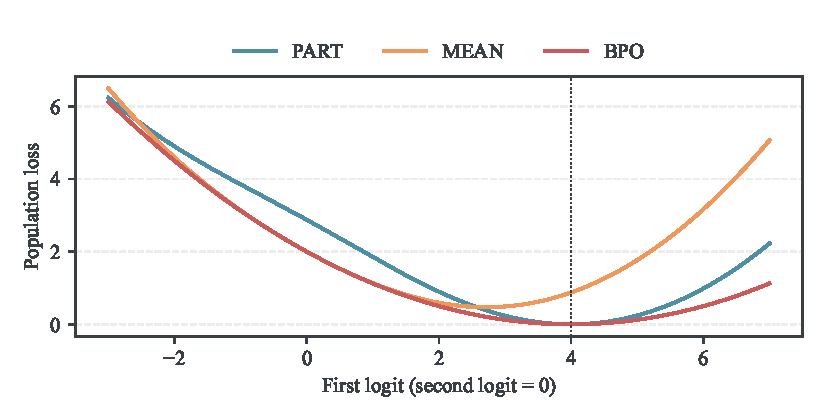
\includegraphics[width=0.96\textwidth]{../../results/book-reconstruction/identities.pdf}
\caption{二元 categorical 分布下三种同尺度回归目标。$q=(1/2,1/2)$、$f=(2,-2)$、$\eta=1$，第二个 logit 固定为零；虚线 $z_1=4$ 对应共同 Gibbs target。Part 与 BPO 的总体零损失位置相同，Mean 的最优点不同。}
\label{evidence:identities-figure}
\end{figure}

% END SOURCE: sections/evidence_reconstruction.tex


% BEGIN SOURCE: book/sections/evidence_toy.tex
\section{可枚举 Token 实验与实现边界}
\label{evidence:toy}

\subsection{实验设置}

实验脚本位于 \path{experiments/toy/toy_token_inner.py}。它只包含一个固定 history 和四个 token：
\begin{equation}
 q_0=(0.62,0.23,0.10,0.05),
 \qquad
 t=(0.08,0.17,0.25,0.50).
\end{equation}
每个方法从同一个初始策略 $p_{0,0}=(0.70,0.15,0.10,0.05)$ 开始，使用 $400$ 步、学习率 $0.15$，完整枚举 vocabulary，不使用 rollout，不使用 sequence-level reward。为核对离开 anchor 后的梯度，这个固定 anchor 实验采用偏离 anchor 的初始化。正式 OPD outer--inner 算法从 $p_{k,0}=q_k$ 开始。PMD-Part 和 PMD-Mean 用 exact weighted squared residual；BPO 使用完整词表下的中心化 residual 平方损失；MDPO 使用 exact categorical Fisher preconditioner。

\subsection{画图实验的输入数据与三层数据集}

本项目的图不能直接从一批混合的 rollout 日志中生成。每一张图都必须注明它使用的是哪一个策略、哪一个 prefix 测度以及哪一种词表访问方式。实验输入按由易到难分为三层。

第一层是可枚举的 categorical oracle。固定一个 prefix $s$，直接生成 anchor、teacher 和 student 的完整 logits，并通过 softmax 得到 $q_k(\cdot\mid s)$、$t(\cdot\mid s)$ 和 $p_{k,n}(\cdot\mid s)$。anchor 可以用随机 logits 加温度生成，teacher 可以通过独立随机 logits 或与 anchor 具有指定 KL 的混合分布生成。每个 prefix 保存完整的概率向量、两个 log-prob 向量以及 exact
\begin{equation}
K_{qt,k}(s)=\operatorname{KL}(q_k\Vert t),\qquad K_{qp,k,n}(s)=\operatorname{KL}(q_k\Vert p_{k,n}),
\end{equation}
和
\begin{equation}
\log Z_k(s)=\log\sum_{v\in\mathcal V}\exp\bigl((1-\eta)\log q_k(v\mid s)+\eta\log t(v\mid s)\bigr).
\end{equation}
这一层不需要文本数据，也不运行模型 rollout；它提供所有估计量的 ground truth，专门用于画 bias、variance、均方误差和梯度误差曲线。

第二层是真实模型产生的 prefix 数据，但仍然冻结 outer step。先选定一个不参与训练的 prompt 文件 $\mathcal X=\{x_i\}_{i=1}^{N_x}$，每个 prompt 只作为输入，不需要人工答案或 reward label。用当前 anchor $q_k$ 对每个 prompt 采样若干条 response，得到
\begin{equation}
s_{i,t}=(x_i,y_{i,<t}),\qquad a_{i,t}=y_{i,t},\qquad a_{i,t}\sim q_k(\cdot\mid s_{i,t}).
\end{equation}
保存 prompt id、token ids、attention mask、response mask、prefix 长度、anchor 对采样 token 的 log-prob，以及 teacher 对同一 token 的 log-prob。KL 或 $\log Z_k$ 的估计不应把不同 prefix 混在一起：同一 prefix 的多个 next-token 样本才能用于估计条件期望；不同 prefix 只能在外层按照经验访问测度 $\widehat d_k$ 聚合。

第三层才是完整的 OPD outer loop。第 $k$ 轮只使用 $q_k$ 生成 rollout，缓存该轮的 prefix 集合和 anchor/teacher 的 token-level log-prob；随后固定这些数据运行 $N$ 个 inner steps，得到 $p_{k,N}$，再执行 hard sync 或 soft sync 得到 $q_{k+1}$。同步后必须重新 rollout，不能把上一轮的 prefix 和旧 anchor log-prob 继续当作新一轮数据。这样得到的序列
\begin{equation}
\{(\widehat d_k,q_k,p_{k,n},t): k=0,\ldots,K_{\mathrm{out}}-1,\ n=0,\ldots,N\}
\end{equation}
才是 outer 动力学图的输入。

图中以 $J$ 表示保留的头部 token 数量。对每个固定 prefix，同时记录 full-vocabulary oracle、sampled-token、top-$J$ 三条估计路径。建议先画以下三组图：

\begin{enumerate}
\item 在第一层 oracle 上，以 $J$ 或同 prefix 样本数 $m$ 为横轴，画 $K_{qt,k}$、$K_{qp,k,n}$ 和 $\log Z_k$ 的 bias、standard deviation、RMSE；
\item 在第二层真实 prefix 上，以 inner step $n$ 为横轴，画 exact-oracle 可用部分的 KL、sampled estimator 的方差、anchor--student 的 $\chi^2$ 或有效样本量；
\item 在第三层 outer loop 上，以 $k$ 为横轴，分别画 teacher KL、mirror-target KL、policy--anchor KL、token-level loss、rollout reward，以及 hard sync 与 soft sync 的差异。
\end{enumerate}

第一层能够完整枚举，并检查每个恒等式。第二层在能取得完整词表打分的 prefix 上同样提供 exact oracle，用于检验真实语言模型长尾词表上的误差与方差。第三层要求先核对目标、估计量和 inner 优化；仅凭一条性能曲线无法区分 OPD 本身、prefix 分布漂移、KL 估计偏差和 inner 优化误差。

\subsection{结果}

表~\ref{tab:toy-results} 区分有限步优化误差、到 Gibbs 分布的距离和总体目标差异。方法 $M$ 的自身最优分布为 $p_0^{\star,M}$，400 步后的 student 为 $p_{0,N}$，$N=400$。PMD-Mean 的最优分布由 Lambert-$W$ 归一化方程求得，其余三种方法的最优分布为 $p_0^{\mathrm G}$。定义
\begin{align*}
e^{\mathrm{opt}}_M&=\operatorname{TV}(p_{0,N},p_0^{\star,M}),\\
e^{\mathrm{Gibbs}}_M&=\operatorname{TV}(p_{0,N},p_0^{\mathrm G}),\\
e^{\mathrm{target}}_M&=\operatorname{TV}(p_0^{\star,M},p_0^{\mathrm G}).
\end{align*}
第一项衡量有限步优化误差，第三项衡量方法总体目标的差异。

\begin{table}[ht]
\centering
\caption{固定测度 token inner 的可枚举实验，400 步后结果。}
\label{tab:toy-results}
\begin{tabular}{llrrr}
\toprule
$\eta$ & 方法 & $e^{\mathrm{opt}}_M$ & $e^{\mathrm{Gibbs}}_M$ & $e^{\mathrm{target}}_M$\\
\midrule
0.25 & PMD-Part & 1.11e-03 & 1.11e-03 & 0.00e+00\\
0.25 & PMD-Mean & 6.81e-04 & 9.26e-03 & 9.12e-03\\
0.25 & BPO & 1.96e-08 & 1.96e-08 & 0.00e+00\\
0.25 & MDPO & 8.33e-17 & 8.33e-17 & 0.00e+00\\
0.50 & PMD-Part & 2.65e-03 & 2.65e-03 & 0.00e+00\\
0.50 & PMD-Mean & 3.58e-04 & 6.86e-02 & 6.85e-02\\
0.50 & BPO & 1.23e-04 & 1.23e-04 & 0.00e+00\\
0.50 & MDPO & 1.25e-16 & 1.25e-16 & 0.00e+00\\
0.80 & PMD-Part & 2.97e-03 & 2.97e-03 & 0.00e+00\\
0.80 & PMD-Mean & 4.11e-05 & 1.90e-01 & 1.90e-01\\
0.80 & BPO & 4.53e-03 & 4.53e-03 & 0.00e+00\\
0.80 & MDPO & 2.78e-16 & 2.78e-16 & 0.00e+00\\
\bottomrule
\end{tabular}
\end{table}

PMD-Mean 到自身最优解的误差随优化下降，但到 Gibbs 解的距离保留了结构性差异。例如 $\eta=0.8$ 时，其有限步优化误差为 $4.11\times10^{-5}$，两个总体最优解的距离为 $0.1904$。继续优化只能消除前者。

BPO 的最优解仍为 Gibbs 分布，但本实验的固定步长与 400 步预算下，$\eta=0.8$ 时尚有 $4.53\times10^{-3}$ 的优化误差。MDPO 使用精确 categorical Fisher 自然梯度，在该四动作问题上达到浮点精度。该结果比较的是指定 optimizer 与预算下的误差，不构成一般模型上的收敛速度排序。

$\eta$ 同时影响 Gibbs target、Mean 的 Lambert-$W$ target 以及各损失的梯度尺度。本节 outer--inner 算法 中 BPO 的 $\eta^{-1}$ 已显式进入梯度权重，实验使用相同学习率时也保留这个尺度，不能把缩放后的方向当作实际梯度。

\subsection{正式 LLM 实验前的数学与实现检查}

在 Pythia-14M/70M 上运行前，代码应先逐项通过以下 oracle tests：

\begin{enumerate}
\item 对随机 categorical logits，核对 Mean 的 Lambert-$W$ 归一化、KKT 条件与最优点梯度；核对 Mean/BPO 的损失及梯度差异恒等式；
\item 对随机 categorical logits，检查 PMD-Part 的 \path{logsumexp} target 与显式求和一致；
\item 对随机 $p,q$，用大量样本检查 K4 value 与 exact $\KL(p\Vert q)$ 的误差按 $O(B^{-1/2})$ 下降；
\item 用 autograd finite difference 检查 K4 gradient，而不是只检查 value；
\item 检查固定 anchor 采样的 importance correction 在 $p/q$ 接近一时无偏；
\item 人为改变 student 与 anchor 的偏离程度，测量 $\chi^2$ 与重要性加权估计方差；增加 inner steps 不保证二者单调上升；
\item hard sync 后重新 rollout，确认新一轮 residual 使用新的 anchor，而不是上一轮缓存的 log-prob。
\end{enumerate}

这些检查完成前不运行大型模型 sweep。当前仓库中的 toy 输出由 \path{toy_token_inner.py}（从仓库根用 \path{PYTHONPATH=src uv run --with torch python} 运行）生成，结果保存在\path{results/toy/toy_token_inner.csv}。独立的 \path{tests/test_kl_estimators.py} 使用 200,000 个 token 样本检查 K4 的 value 与 autograd gradient；旧书记录的绝对 value 误差为 $5.6\times10^{-5}$，gradient 的 $\ell_2$ 误差为 $1.5\times10^{-3}$。

\path{tests/test_mean_bpo.py} 的旧版修订核验记录覆盖 48 组随机问题：词表维数为 2、4、8，镜像系数为 0.1、0.5、1、2。核验对象包括解析梯度、逐坐标有限差分、Mean/BPO 损失及梯度恒等式、Mean 归一化与 KKT 条件、最优点驻点、Part/BPO 的 Gibbs 零损失、初始化方向尺度、恒定信号、完整枚举的有限样本修正与 off-behavior 双样本权重。该记录与 toy 实验分别检验推导正确性和有限步优化行为；这里保留历史配置，不将其写成合并时重新运行的测试。

\section{真实语言模型上的四种 \texorpdfstring{Top-$J$}{Top-J} 对照}

为了把KL 估计章的四个数学对象放回 OPD 场景，我们使用 GSM8K test 的全部 1,319 个 prompt。Student 为 Qwen3-1.7B，Teacher 为 Qwen3-4B，温度固定为 $1.0$；每个 prompt 生成一条完整 student rollout。对 rollout 的每个 prefix，打分阶段计算 student 与 teacher 的完整词表分布，随后只保存汇总量和审计样本。打分采用 NF4 权重量化、bf16 计算，因此这里的 full-vocabulary KL 是该量化模型对的 oracle。生成采用 bf16 vLLM，其 sampled token 来自与 NF4 打分略有不同的 proposal；EMA 的理论方差严格按 NF4 student 分布计算，观测误差另行报告。总计得到 350,166 个 prefix。实验元数据、逐 $J$ 汇总和绘图脚本分别位于 \path{results/qwen3_gsm8k_pair_kl/metadata.json}、 \path{results/qwen3_gsm8k_pair_kl/kl_summary_by_k.csv} 和 \path{experiments/plotting/plot_pair_kl.py}。

令 $S_J$ 为 student 概率的 top-$J$ 支持集。表~\ref{tab:qwen-topk-four} 中的 bias 和 RMSE 都相对于同一 prefix 上的完整
\begin{equation}
 \mathcal K^{\mathrm{full}}(s)=\KL\bigl(p_{k,n}(\cdot\mid s)\Vert t(\cdot\mid s)\bigr)
\end{equation}
计算。Truncated、Normalized 和 Tail-Aware 的条件采样方差恒为零；EMA Top-$J$ 的 variance 是一个尾部 sampled token 修正的理论条件方差。四种方法使用完全相同的 prefix 和 student 支持集，没有额外增加每个 prefix 的采样数。Tail-Aware 尾部质量在 float64 下直接累加，避免头部质量接近一时用 $1-P_J$ 相减丢失精度。审计样本同时保存 teacher 在该支持集上的质量 $Q_J$ 与 Tail-Aware 值。

\begin{table}[ht]
\centering
\small
\caption{Qwen3-1.7B student 与 Qwen3-4B teacher 在 GSM8K rollout prefix 上的 Top-$J$ KL 统计。EMA 的 RMSE 是理论 sampled-tail RMSE；Normalized 的 $J=0$ 未定义。}
\label{tab:qwen-topk-four}
\begin{tabular}{rrrrrrr}
\toprule
$J$ & $P_J$ & $\mathrm{bias}_{\mathrm{trunc}}$ & $\mathrm{RMSE}_{\mathrm{trunc}}$ & $\mathrm{RMSE}_{\mathrm{EMA}}$ & $\mathrm{bias}_{\mathrm{norm}}$ & $\mathrm{RMSE}_{\mathrm{norm}}$\\
\midrule
0  & 0       & -0.26932 & 1.03968 & 0.80948 & --       & --\\
1  & 0.94208 & -0.07672 & 0.39307 & 0.68557 & -0.26932 & 1.03968\\
2  & 0.98676 & -0.02187 & 0.15337 & 0.40189 & -0.08392 & 0.54660\\
4  & 0.99747 & -0.00465 & 0.04761 & 0.18864 & -0.02629 & 0.28804\\
8  & 0.99949 & -0.00094 & 0.01416 & 0.08308 & -0.00874 & 0.15007\\
16 & 0.99988 & -0.00023 & 0.00488 & 0.03959 & -0.00310 & 0.08367\\
32 & 0.99996 & -0.00008 & 0.00217 & 0.02249 & -0.00127 & 0.05438\\
\bottomrule
\end{tabular}
\end{table}

\begin{figure}[ht]
\centering
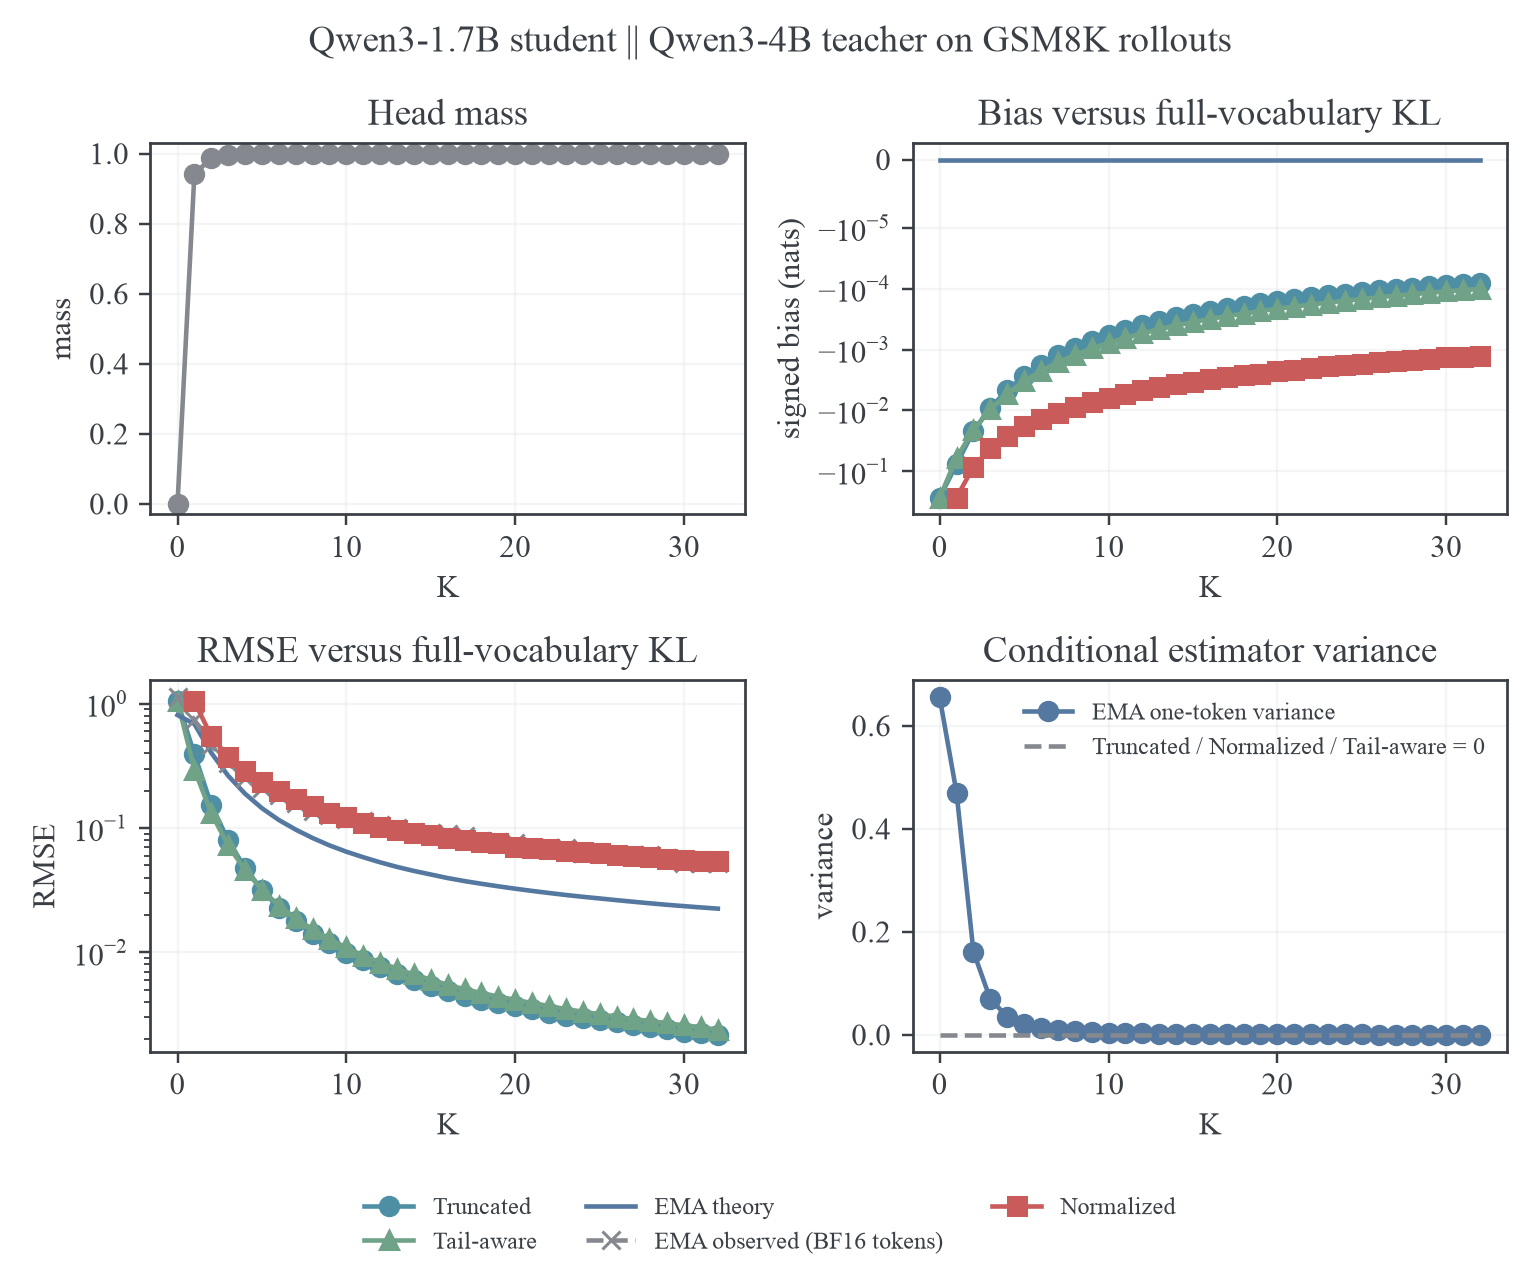
\includegraphics[width=0.96\textwidth]{../../results/qwen3_gsm8k_pair_kl/pair_kl_topk_metrics.png}
\caption{真实 GSM8K rollout 上四种 Top-$J$ KL 的误差曲线。bias 保留正负号；variance 是固定 prefix 的条件采样方差，不是不同 prefix 之间的数值方差。EMA observed 使用 bf16 rollout token，与 NF4 打分分布的理论曲线分开。}
\label{fig:qwen-topk-four}
\end{figure}

结果体现了四种定义之间的结构性差异。首先，student 的 top-$J$ 质量在 $J=4$ 时已经达到 $0.99747$，在 $J=32$ 时达到 $0.99996$，所以截断项的偏差和 RMSE 很快下降。其次，EMA Top-$J$ 在任何 $J$ 上都保持理论无偏，但只要尾部 log-ratio 的二阶矩仍然较大，sampled correction 就会带来明显方差；在 $J=32$ 时它的理论 RMSE 仍为 $0.02249$，高于截断项的 $0.00217$。这不是无偏性失效，而是典型的 bias--variance trade-off。

Normalized Top-$J$ 的行为不同。$J=1$ 时两边都是同一个 point mass，局部 KL 在数学上等于零，因此相对于完整 KL 的 bias 为 $-0.26932$。随着 $J$ 增大，条件分布逐渐包含更多质量，RMSE 从 $1.03968$ 降至 $0.05438$；但在 $J=32$ 时仍明显高于截断项。这说明归一化修复的是局部目标的概率尺度，而不是尾部 token-wise KL。它适合作为 dense local OPD 目标，却不能被解释为完整 KL 的高精度估计量。

Tail-Aware 的全量结果见表~\ref{tab:qwen-tail-aware}。其 RMSE 随 $J$ 单调下降，符合KL 估计章的支持集细化定理。在 $J=1,2,4$ 时，其 RMSE 小于 Truncated；在 $J=8,16,32$ 时，Truncated 略小。这正对应尾部质量项与尾部形状项的抵消：Tail-Aware 恢复质量项后，剩下的误差严格为非正的尾部形状偏差，而 Truncated 的两个遗漏项可以部分相互抵消。这个标量 RMSE 排序不等于训练稳定性的排序，也不能作为四种 OPD 训练方法最终性能的结论。

\begin{table}[ht]
\centering
\caption{同一批 350,166 个 prefix 上补全的 Tail-Aware 结果。条件采样方差在所有 $J$ 上均为零。}
\label{tab:qwen-tail-aware}
\begin{tabular}{rrrr}
\toprule
$J$ & mean Tail-Aware KL & bias & RMSE\\
\midrule
0 & 0 & -0.269321 & 1.039683\\
1 & 0.209759 & -0.059561 & 0.295078\\
2 & 0.248414 & -0.020907 & 0.131407\\
4 & 0.263978 & -0.005343 & 0.045886\\
8 & 0.268091 & -0.001230 & 0.015303\\
16 & 0.269006 & -0.000315 & 0.005493\\
32 & 0.269220 & -0.000101 & 0.002391\\
\bottomrule
\end{tabular}
\end{table}

这组实验不能支持“所有情况下都应该使用 normalized Top-$J$”这一结论。它支持更精确的选择规则：当我们需要在有限支持集上构造稳定的多 token 蒸馏 reward 时使用 $\mathcal K_J^{\mathrm{norm}}$；当我们需要完整 vanilla OPD KL 的估计时使用 EMA Top-$J$；当我们希望保留尾部总质量、又不承受 sampled correction 的方差时使用 Tail-Aware Top-$J$；Truncated Top-$J$ 则作为低方差、有明确尾部偏差的基线。

% END SOURCE: sections/evidence_toy.tex


% BEGIN SOURCE: book/sections/evidence_hard_sync.tex
\section{Hard sync 的有限词表数值核验}
\label{dyn:sec:hard-sync-experiments}

本节用完全可求解的 categorical 子问题核验前述动力学。实验程序为 \path{experiments/toy/hard_sync_audit.py}，结果保存在 \path{results/hard-sync-audit/}。所有计算使用 float64，随机种子为 $20261010$。这是固定 prefix 下的分布空间实验；其证据范围是精确更新与受控输出扰动，LLM 的参数共享、随机梯度和 rollout 变化需要分别测量。

\subsection{实验问题与可证伪的判据}

实验在运行前固定以下判据。
\begin{enumerate}
 \item Gibbs 的跨度递推与三点 KL 恒等式应在数值误差内成立。词表大小取 $2,4,8$，每个大小生成 $12$ 组独立正分布，步长取 $0.2,0.8,1,1.2,1.8,2,2.2$，共检查 $252$ 个更新。绝对残差阈值取 $10^{-12}$。
 \item 独立 SciPy Lambert-$W$ 求解器与仓库 \path{token_inner.mean_target} 的 $36$ 组输出逐坐标差不超过 $10^{-12}$。各步长的 Mean KKT 残差与归一化残差也不超过 $10^{-12}$。这同时检查理论更新与参考实现的对应关系。
 \item 固定 $t=(0.2,0.3,0.5)$、$z=(-1,0.2,0.8)$，令 $q_\epsilon\propto t\exp(\epsilon z)$。扫描 $\epsilon=0.4,0.2,0.1,0.05,0.02,0.01$，Mean 在 $\eta=1$ 时的 KL 三次比值应趋于一；最小 $\epsilon$ 的相对偏差阈值为 $2\%$。
 \item 同一 teacher 下，从 $q_0\propto t\exp(0.2z)$ 出发，运行 $\eta=2$ 的 $10000$ 轮精确更新。Gibbs 应保持二周期，Mean 的 $k\KL(q_k\Vert t)$ 应接近 $1/16$；最终绝对偏差阈值为 $0.004$。
 \item 输出噪声和 reward 噪声分别按式~\eqref{dyn:eq:hs-centered-linear} 注入。用 $20000$ 条独立路径、$240$ 步以及 $\eta=0.2,0.5,1,1.5,1.8$，比较 teacher 加权二阶矩的样本均值和精确有限时间预测。每个均值须落在预测值的五个 Monte Carlo 标准误差以内。
\end{enumerate}

\subsection{数值稳定性与局部阶数}

KL 三次收敛会迅速产生接近机器精度的 KL。直接计算 $\sum_a p_a\log(p_a/t_a)$ 会把一阶正负项相消，影响三次比值。令 $d_a=p_a/t_a-1$，归一化给出 $\sum_a t_ad_a=0$，因此改写为
\begin{equation*}
 \KL(p\Vert t)=\sum_a t_a\{(1+d_a)\log(1+d_a)-d_a\}.
\end{equation*}
当 $|d_a|<10^{-3}$ 时，程序使用
\begin{equation*}
 (1+d)\log(1+d)-d
 =\sum_{n=2}^{9}\frac{(-1)^n d^n}{n(n-1)}+O(d^{10}).
\end{equation*}
这保留局部 KL 的二阶首项。Mean 归一化根也用 $\E_q\operatorname{expm1}(G-W_0(\lambda e^G))=0$ 求解，避免两个接近一的数相减。求根器同时记录 KKT 残差。

本方向的 teacher 方差与跨度为
\begin{equation*}
 \Var_t(z)=0.4644,\qquad \operatorname{osc}z=1.8,
\end{equation*}
所以理论预测
\begin{equation*}
 \frac{b(p^\star,t)}{b(q_\epsilon,t)^3}\to
 \frac{0.4644}{2\cdot1.8^2}=0.071666\ldots.
\end{equation*}
逐点数值与 KL 三次比值保存在 \path{cubic.csv}；它们检验乘子的二阶修正，而非仅检验一次线性化。

预设的各项数值判据均通过。表~\ref{dyn:tab:hard-sync-audit} 汇总残差与局部、边界常数；这里的实测值来自上述固定配置。
\begin{table}[htbp]
 \centering
 \caption{精确 hard-sync 更新的数值核验。}
 \label{dyn:tab:hard-sync-audit}
 \begin{tabular}{ll}
 \toprule
 项目 & 实测结果\\
 \midrule
 Gibbs 三点恒等式最大绝对残差 & $1.78\times10^{-15}$\\
 Mean 独立求解与参考实现最大坐标差 & $2.78\times10^{-16}$\\
 Mean KKT 与归一化最大残差 & $3.55\times10^{-15}$\\
 $\epsilon=0.01$ 的 KL 三次比值 & $1.011557$，极限为 $1$\\
 同一点的跨度三次比值 & $0.071591$，极限为 $0.071667$\\
 $\eta=2$、$k=10000$ 的 Mean $k\KL$ & $0.062303$，极限为 $0.0625$\\
 \bottomrule
 \end{tabular}
\end{table}

\subsection{边界阻尼与噪声位置}

图~\ref{dyn:fig:hard-sync-audit} 左侧比较同一初值下的边界步长：Gibbs 的两周期与 Mean 的缓慢衰减清楚分离。虚线是独立推导的 $1/(16k)$，并未用实验数据拟合。

右侧从零误差出发，先生成独立 $N(0,\sigma^2I)$ 向量，再减去其 teacher 均值，取 $\sigma=0.01$。该居中噪声满足
\begin{equation*}
 \E\|\xi\|_t^2=\sigma^2\left(1-\sum_a t_a^2\right).
\end{equation*}
对固定输出噪声，有限时间精确预测为
\begin{equation*}
 \E\|y_K\|_t^2=
 \sigma^2\left(1-\sum_a t_a^2\right)
 \frac{1-(1-\eta)^{2K}}{\eta(2-\eta)}.
\end{equation*}
对于 reward 噪声，再乘 $\eta^2$。图中误差条是均值的 $1.96$ 个标准误差，虚线是上述预测。两个噪声模型呈现不同步长趋势，与输入位置的理论分析一致。

\begin{figure}[htbp]
 \centering
 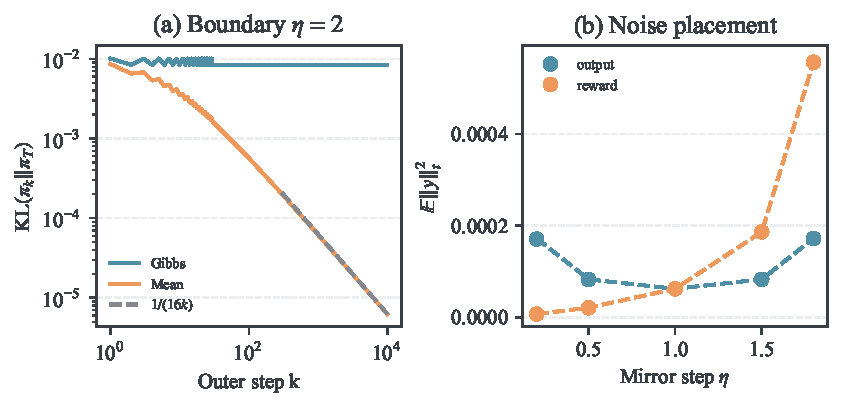
\includegraphics[width=0.96\textwidth]{../../results/hard-sync-audit/hard-sync.pdf}
 \caption{固定三元词表下的 hard-sync 审计。左：$\eta=2$ 的精确 Gibbs 与 Mean teacher KL；右：固定输出噪声和固定 reward 噪声的 teacher 加权二阶矩。点和实线来自数值更新，虚线来自独立理论预测。}
 \label{dyn:fig:hard-sync-audit}
\end{figure}

实验中的浮点求根和有限时间误差不替代证明。相反，精确恒等式、局部阶数、边界常数与随机二阶矩分别给出四类独立的数值约束，使实现错误能被具体定位。配置、源码版本、脚本校验和及最大残差记录在 \path{metadata.json}，完整复现命令与逐项结果见实验报告。

% END SOURCE: sections/evidence_hard_sync.tex


% BEGIN SOURCE: book/sections/evidence_baseline.tex
\section{Pythia baseline 实验记录}
\label{subsec:ch2-opd-baseline-results}

本节完整保留旧书记录的配置和数值。当前重构核验未找到能逐项追溯此表的原始运行目录，因此它属于历史实验记录；本次重新运行的证据单独列于第八章开头，不能用本表替代缓存或同步逻辑的源码测试。

实验使用 Pythia-14M student、Pythia-70M teacher、WikiText validation prefixes、 top-$J=32$ anchor support、温度 $1.0$、response length $64$、batch 中 $1024$ 有效 token、learning rate $10^{-6}$ 和 seed $42$。两条训练均运行 $32$ 个 outer step；on-policy 每轮只更新一次，token-IS 每轮复用同一 rollout 做 $4$ 个 inner step。评估在固定的 $8128$ 个 prefix 上使用 float32 full-vocabulary teacher forcing， 该指标采用固定 prefix 上的完整求和，与训练时 sampled action 噪声区分。

\begin{center}
\small
\setlength{\tabcolsep}{3pt}
\begin{tabular}{lrrrrrr}
\toprule
方法 & inner $N_{\mathrm{inner}}$ & 初始 $\KL(p\Vert t)$ & 最终 $\KL(p\Vert t)$ & 初始 $\KL(t\Vert p)$ & 最终 $\KL(t\Vert p)$ & 最终 ESS fraction\\
\midrule
On-policy OPD & $1$ & 0.9873 & 0.9356 & 0.8907 & 0.8921 & 1.0000\\
Token-IS OPD & $4$ & 0.9873 & 0.9094 & 0.8907 & 0.9387 & 0.9335\\
\bottomrule
\end{tabular}
\end{center}

历史记录中两种方法都降低了 $\KL(p\Vert t)$。Token-IS 的 $\KL(p\Vert t)$ 降得更多，但 $\KL(t\Vert p)$ 上升，且 ESS 降至约 $93.35\%$；本配置同时改变了数据复用和每轮更新预算，因而这组差异不能单独归因于 stale rollout。历史记录中的 score coefficient RMS 约为 $2.9$--$3.1$，而梯度裁剪前的 norm 约为 $1.6\times10^3$--$2.1\times10^3$。这个尺度差异要求单独核查优化尺度和混合精度配置；32 步记录不提供长期速度排序。此外，旧配置里的 \path{model_dtype=float32} 只约束权重加载；若未显式设置 FSDP \path{mixed_precision}，前向仍可能采用 BF16 autocast。正式比较应把这一项写入 resolved config，并同时记录 \path{dtype}、梯度裁剪、ESS 和 full-vocabulary 固定前缀指标。

% END SOURCE: sections/evidence_baseline.tex


% BEGIN SOURCE: book/sections/evidence_resopd.tex
\section{ResOPD 实现与论文实验}
\label{sec:resopd-implementation}

本节沿用前文的 $\ell_v$、score $\psi_v$、头部向量 $h_g$、尾部均值 $\mu_g$ 与事件 $J_A$，将控制族对应到公开训练实现。\footnote{论文来源为 \href{https://arxiv.org/abs/2610.04882}{ResOPD}；本仓库保存的全文为 \path{docs/papers/2610.04882_zh_CN/}。代码来源为 \href{https://github.com/InternLM/ResOPD}{InternLM/ResOPD}。}

\subsection{代码调用链与停止梯度}

开源仓库没有单独的 ``HETS'' loss mode；HETS 是论文中的比较基线。发布代码注册的唯一新模式是 ``resopd''，而 sampled-token、Top-$k$ 和普通 ``k1/k2/k3'' 路径属于其他 loss mode。

teacher 路径从 \path{verl/experimental/teacher_loop/teacher_manager.py} 开始。选择 ``loss\_mode=resopd'' 后，vLLM 必须返回 teacher Top-$J$ 的 token ids/log-probs，以及实际 student token 的 teacher log-prob。

\path{verl/workers/rollout/vllm_rollout/prompt_logprobs.py} 保存两组字段：
\begin{itemize}
\item 头部支持：\path{prompt_ids} 与 \path{prompt_logprobs}。
\item 实际动作：\path{sampled_prompt_ids} 与 \path{sampled_prompt_logprobs}。
\end{itemize}
实际动作的 teacher log-prob 即使落在 Top-$J$ 之外也必须保留。

student logits 经 \path{verl/trainer/distillation/fsdp/losses.py} 对齐后，\path{verl/trainer/distillation/losses.py} 将四个 payload 送入 \path{verl/trainer/distillation/resopd.py} 的 \path{resopd_loss}。该 kernel 的数学对应关系如下：
\begin{enumerate}
\item 完整 student logits 做 log-softmax，得到头部 $P(v)$、$\ell_v$ 和 $P_S$；teacher Top-$J$ log-prob 在进入计算时 detach。
\item 从实际 token 得到 $\ell_A$，并用 \path{student_tail_mass}、\path{teacher_tail_mass} 构造 $\log(\tau_P/\tau_Q)$。
\item 用 \path{support_score} 计算 $b_{\mathrm{TA}}$，并令 \path{centered_event} 等于 $\mathbf 1\{A\in S\}-P_S$。
\item 通过 \path{surrogate - surrogate.detach()} 保留 forward 数值、替换 backward，得到式~\eqref{est:eq:chapter3-control-family} 中 $b=b_{\mathrm{TA}}$ 的特例。
\end{enumerate}
实现中的 teacher 数值、事件系数和控制项均停止梯度。仓库 docstring 明确说明返回值不是确定性 KL 目标，单个 forward value 可以为负；应审计 backward 梯度、期望和协方差，而不是把 loss 平均值解释成完整 KL。

无偏性要求 $A$ 来自当前完整 student 分布，或按 KL 梯度估计章给出的重要性权重校正。发布脚本使用温度 $1$、\path{top_p=1}、\path{top_k=-1}。论文的主要数学实验使用温度 $1$、\path{top_p=0.95}、\path{top_k=20}；全支持审计与跨领域实验采用完整祖先采样。这些设置必须分别报告：重新计算未截断 logits 能恢复目标概率 $P$，不能把已生成动作的测度 $\beta$ 改回 $P$。

\subsection{公开实验与 baseline}

论文的基线可按目标分成三组。第一组是有偏确定性 Top-$k$ 方法：Teacher Top-$k$ fKL、Teacher Top-$k$ rKL 和 TA-OPD（尾部伪 token 的粗粒度 KL）。第二组是无偏 reverse-KL 梯度 estimator：Sampled-token OPD、教师 Top-$k$ 支持上的 vOPD、HETS 和 ResOPD。第三组是机制消融：支持大小 $J\in\{1,4,16,32,64\}$、完整祖先采样与 top-$p$/top-$k$ 截断、学习率敏感性，以及统一双控制族中的 SC-TA（$\vartheta=1$；ResOPD 为 $\vartheta=0$）。

冻结 prefix 审计在 GSM8K、HMMT26 和 DeepMath 上枚举完整动作，报告梯度协方差迹和 NSR。Top-$4$ 下，论文报告 ResOPD 相对 sampled-token OPD 降低 $52.5\%$--$75.0\%$ 的协方差迹，并在五个面板中优于 HETS。端到端数学实验使用 Qwen3.5-27B 教师和 Qwen3.5-4B 学生，评估 DeepMath、AIME26、HMMT26、OlymMATH；科学/代码迁移使用 Qwen3-30B-A3B-Instruct 到 Qwen3-4B，评估 GPQA-D、SuperGPQA、LiveCodeBench v5/v6。论文报告数学平均分 ResOPD $50.12\%$、HETS $45.72\%$，迁移平均分 ResOPD $44.15\%$、HETS $43.63\%$。

仓库公开了可直接运行的 DeepMath 子集：1,024 条训练样本和 252 条 held-out 样本；入口为 \path{examples/resopd/run_resopd.sh}，默认 FSDP2 student、vLLM teacher、Top-$4$、full-support rollout。\path{tests/resopd} 包含 estimator、teacher payload 和 verl integration 检查，发布验证记录 22 个 standalone 与 13 个 integration checks。

需要避免的概念混淆是：HETS 是稀疏 rKL 梯度基线，不是 PPO 的 value baseline；ResOPD 的 $b_{\mathrm{TA}}$ 是 control variate。仓库中普通 verl 的 ``k1/k2/k3'' KL penalty、GRPO、RLOO、ReMax 等属于框架通用路径，并非论文中同一 teacher payload 下的 HETS/ResOPD 方差基线。

% END SOURCE: sections/evidence_resopd.tex


% BEGIN SOURCE: book/sections/evidence_scalar_schedule.tex
\section{固定监督下的标量调度验证}
\label{evidence:scalar}

2026 年 10 月 12 日的验证包括 690 条可控二次轨迹、540 条共享分类模型轨迹，以及 GPU 0--3 上的 20 条 DeepSeek 1.5B 固定 prefix 轨迹。二次与分类模型各条件采用五个种子。语言模型固定 13 条 DAPO prompt、416 个 q-sampled prefix，缓存、teacher、anchor 和 $\eta=0.3$ 在 inner 中冻结；短 response 和 prompt 截断用于优化验证，未进行数学正确率评测。

完整 BPO 的 FP32 分支中，沿标准 AdamW 方向作三点 forward 搜索，在初始目标的 $0.1\%$ 阈值上用 117 次 backward，常数 lr 网格中最快分支为 131 次。对应累计 forward 分别为 469 与 133，耗时分别约为 82.3 与 43.6 秒。搜索减少 10.7\% backward，增加总运行时间。搜索在第 117 步之后至第 500 步保持低于该阈值；常数网格中最早保持到终点的分支为 251 步。该保持口径是有限预算内的反弹审计，不能推广为无限步稳定性。

搜索未固定后期相对吸收率。三个 50 步窗口的平均 log 收缩率从 0.0612 降到 0.0108，再降到 0.00184。该结果符合第~\ref{dyn:scalar} 节的方向能力限制。方向搜索更好地匹配当前位置的稳定步幅，没有把共享参数的慢谱消除。

生产 Top-16 加尾部桶、固定 sampled action 的分支表现出经验 residual 与完整 BPO 的失配。默认常数 lr 下，120 步后经验平方 residual 为初始的 0.0115\%，完整 BPO 仍为初始的 62.7\%。提高 lr 可进一步恶化完整误差。经验 residual 搜索的完整误差终值为初始的 43.0\%，而更小的常数 lr 已达到 44.1\%；搜索额外 forward 成本未得到对应的总时间收益。用完整误差接受步长但保持生产 surrogate 方向的分支有 36 次拒绝，说明标量无法替代缺失的下降方向。

原始轨迹、逐条件 CSV、forward/backward 计数及图像位于仓库的 \texttt{results/scalar-schedule/}。固定 token IDs 和 attention mask 已版本化，可以重建 full-vocabulary cache；具体复现命令和生产更新场的分解维护在对应的 BPO 标量调度实验报告中。当前证据支持完整目标上的条件性步长改进，尚未支持现有 sampled/Top-k 生产更新的普遍加速。

% END SOURCE: sections/evidence_scalar_schedule.tex


% END SOURCE: chapters/08_evidence.tex


% BEGIN SOURCE: docs/chapters/09_proximal_families.tex
\chapter{幂均值 MirrorOPD：目标、镜像更新与方差控制}
\label{ch:proximal-families}

本章研究单教师、每个 prompt 一条 rollout、冻结锚点和 BPO 内层的 MirrorOPD。形状参数 $\kappa$ 改变学生与教师之间的目标分布；插值强度 $\eta$ 决定教师参与程度。推导围绕四个动作组织：构造 target、识别精确镜像目标、拟合 target、控制条件采样误差。前六节给出算法主线及形状选择的结论；后三节给出估计器、高维动力学和适用边界。所有条件分布定理都注明冻结测度、正支持和精确更新要求。

\section{单教师问题与统一条件}
\label{sec:power-setup}

% BEGIN SOURCE: book/sections/proximal_setup.tex
\subsection{冻结锚点、教师与当前学生}

教师分布为 $T(a\mid s)$，本轮冻结学生锚点为 $q_n(a\mid s)$，当前 inner 学生为 $p_{n,j}(a\mid s)=\pi_{\theta_{n,j}}(a\mid s)$。固定一个前缀 $s$ 时省略条件及索引，写成 $T,q,p$。词表 $\mathcal V$ 有限；本章的精确分布定理要求 $q_a,T_a,p_a>0$ 且各自归一化。两个基本概率比为
\begin{equation}
 \rho_a=\frac{T_a}{q_a},\qquad r_a=\log\rho_a,\qquad
 U_\theta(a)=\log\frac{p_\theta(a)}{q_a},\qquad
 C_qh=h-\E_qh.
 \label{eq:power-chapter-ratios}
\end{equation}
对每个 prompt 槽位仅生成一条 $y\sim q_n(\cdot\mid x)$，再冻结所得到的有效前缀及归一化权重，形成经验测度 $\widehat d_n$。一个 batch 可以含 $B$ 个 prompt 槽位；$B$ 不表示同一 prompt 的候选组数。每个前缀可用完整词表求和或辅助 action 抽样来计算损失，辅助 action 不等于新增完整 response。

\begin{center}
\begin{tabular}{lp{108mm}}
\toprule
记号 & 含义与更新时点\\
\midrule
$\kappa\in[0,1]$ & 幂均值 target 的形状；同一理论迭代中固定\\
$0<\eta<1$ & 教师插值强度；也是该 target 的精确 MD 步长\\
$\tau$ & 固定教师目标后可另选的 MD 步长，通常 $0<\tau\le\eta$\\
$\alpha_{\mathrm{opt}}$ & 实际 BPO 参数优化器的步长，与 $\eta,\tau$ 区分\\
$\gamma_j,\xi_j$ & 理想 BPO 的 logit 松弛系数和累计拟合进度\\
$\zeta$ & 辅助 action 提案中教师的混合权重\\
$N,I,M,J$ & outer 预算、每轮 inner 次数、辅助 action 数、保留 head 大小\\
\bottomrule
\end{tabular}
\end{center}

本章统一使用 $\eta$。早期解析图中的 $\lambda$、亲和度 $A$、拟合进度 $\beta$ 和连续时间 $\tau$，分别对应正文的 $\eta,a,\xi,t$。边界 $\eta=1$ 时所有 target 都为 $T$；$\eta=0$ 只用于极限或不更新的参照，不代入含 $1/\eta$ 的 BPO 损失。本轮 $q_n,T,\widehat d_n$ 和教师信号全部停止梯度，学生条件中心在每次 inner 重新计算。外层结束后才将拟合后的学生用作下一轮锚点。

\subsection{目标构造、镜像下降与 BPO 拟合的关系}

幂均值框架中有五个不同角色。重心散度 $D_\kappa$ 定义中间 target $m$；教师目标 $\mathcal J_{\kappa,\eta}$ 解释精确外层 MD；$\KL(p\Vert q)$ 保留负熵 mirror 几何；BPO 用冻结 $q$ 拟合 $m$；教师中心 $K_{\kappa,\eta}$ 将条件监督均值归零。重心问题与 BPO 的最小点是本轮 $m$，教师目标 $\mathcal J$ 的最小点是固定 $T$，KL 正则的最小点是 $q$。$m$ 是向教师目标执行一次 mirror 更新的结果，不是 $\mathcal J$ 的全局最小点；$K$ 在 inner 中则只是冻结中心。

\begin{figure}[H]
 \centering
 \begin{tikzpicture}[every node/.style={font=\small},node distance=13mm]
  \node[draw,rounded corners,align=center,text width=35mm] (source) {本轮冻结分布\\学生 $q_n$、教师 $T$};
  \node[draw,rounded corners,align=center,text width=37mm,right=10mm of source] (target) {幂均值 target $m_n$\\重心 $D_\kappa$；MD 目标 $\mathcal J$};
  \node[draw,rounded corners,align=center,text width=35mm,right=10mm of target] (fit) {BPO 拟合\\当前学生 $p_{n,j}$};
  \node[draw,rounded corners,align=center,text width=35mm,below=of source] (roll) {每个 prompt 一条 rollout\\冻结前缀测度 $\widehat d_n$};
  \node[draw,rounded corners,align=center,text width=37mm,below=of target] (loss) {冻结 $q_n$ 的条件方差\\$\Var_{q_n}[\log(p/m_n)]/(2\eta)$};
  \node[draw,rounded corners,align=center,text width=35mm,below=of fit] (sync) {完成本轮 inner\\同步 $q_{n+1}=p_{n,I}$};
  \draw[->] (source) -- node[above]{$\kappa,\eta$} (target);
  \draw[->] (target) -- node[above]{监督} (fit);
  \draw[->] (source) -- node[right]{$y\sim q_n$} (roll);
  \draw[->] (roll) -- node[above]{权重} (loss);
  \draw[->] (loss) -- (fit);
  \draw[->] (fit) -- (sync);
 \end{tikzpicture}
 \caption{单教师、单 rollout 的主线。中间分布是监督 target；response 仍由学生锚点生成。精确求到 target 与神经网络有限步拟合分别承担外层和内层的数学条件。}
 \label{fig:divergence-map-roles}
\end{figure}

\subsection{小插值强度与重尾监督的区别}

对固定随机向量 $X$，$\Var(\eta X)=\eta^2\Var(X)$，其均值也缩小为 $\eta\E X$。若均值非零，相对噪声 $\Var(\eta X)/\|\eta\E X\|^2$ 不变。当前 BPO 损失带 $1/\eta$，其几何端点起始下降方向是 $\E_q[(C_qr)\psi_q]$，不会随 $\eta$ 整体缩小。减小教师参与程度与压制极端概率比是不同操作。

取二元词表 $q=(v,1-v)$、$T_\epsilon=(\epsilon,1-\epsilon)$，其中 $0<v<1$、$v\ne1/2$。对第一个 categorical logit，$\psi_q(1)=1-v$、$\psi_q(2)=-v$。令
\begin{equation}
 r_1=\log(\epsilon/v),\qquad r_2=\log[(1-\epsilon)/(1-v)],\qquad D=r_1-r_2.
\end{equation}
精确条件中心化给出 $C_qr(1)=(1-v)D$、$C_qr(2)=-vD$。单 action 梯度 $X=(C_qr)\psi_q$ 分别取 $(1-v)^2D$、$v^2D$，因此
\begin{align}
 \E_qX&=v(1-v)D,\\
 \Var_qX&=v(1-v)(1-2v)^2D^2.
 \label{eq:proximal-binary-variance}
\end{align}
$D=\log\epsilon+O(1)$，所以 $\Var_qX\to\infty$，任意固定 $\eta>0$ 也不能使 $\eta^2\Var_qX$ 具有分布无关界。这个反例已有精确 baseline 和有界 score。$v=1/2$ 时中心化后的二元 score 梯度恰为常数，必须用非对称的 $q$ 才能证明梯度方差发散。

本章的改进方向是改变冻结教师信号的形状，使负尾部饱和，同时保留局部教师差异的尺度。后续要分别证明固定正 $\eta$ 下的界、$\eta\to0$ 的统一界、残差趋零的噪声界，以及完整参数梯度所需的 score 条件。

% END SOURCE: sections/proximal_setup.tex


\section{幂均值目标与散度重心}
\label{sec:proximal-barycenters}

% BEGIN SOURCE: book/sections/proximal_divergence_map.tex
\label{sec:proximal-divergence-map}

KL 本身属于 $f$ 散度。这里用规范化生成函数固定方向，再推导学生与教师的重心。

\subsection{生成函数与散度方向}

对凸函数 $g:(0,\infty)\to\mathbb R$、$g(1)=0$，定义 Csisz\'ar $f$ 散度
\begin{equation}
 D_g(P\Vert Q)=\sum_a Q_a g(P_a/Q_a).
 \label{eq:divergence-map-csiszar}
\end{equation}
其中采样或求和参照分布是第二个自变量 $Q$。加上任意线性项 $c(x-1)$ 不改变散度，因为 $\sum Q(P/Q-1)=0$。下面采用 $g(1)=g'(1)=0$ 的规范化生成函数；规范化不改变 KL 方向。

概率坐标中的梯度代表可以相差常数向量。切向量 $v$ 满足 $\sum_av_a=0$，所以 $\langle c\boldsymbol1,v\rangle=0$。用规范化透视函数与用单纯形上等价的简化散度表达式求导时，须保留这个差别；MD 一阶条件的乘子和 Fisher 中心化都会消去该常数。

\begin{theorem}[幂散度的 $f$ 表示、对偶与 KL 端点]
\label{thm:divergence-map-power}
设 $0<\kappa<1$，定义
\begin{equation}
 g_\kappa(x)=\frac{\kappa x+1-\kappa-x^\kappa}{\kappa(1-\kappa)}.
 \label{eq:divergence-map-power-generator}
\end{equation}
则 $g_\kappa(1)=g_\kappa'(1)=0$、$g_\kappa''(x)=x^{\kappa-2}>0$，且
\begin{equation}
 D_{g_\kappa}(P\Vert Q)
 =\frac{1-\sum_a P_a^\kappa Q_a^{1-\kappa}}{\kappa(1-\kappa)}
 =D_\kappa(P\Vert Q).
 \label{eq:proximal-power-divergence}
\end{equation}
生成函数的连续端点为
\begin{align}
 g_0(x)&=x-1-\log x,&D_0(P\Vert Q)&=\KL(Q\Vert P),\\
 g_1(x)&=x\log x-x+1,&D_1(P\Vert Q)&=\KL(P\Vert Q).
 \label{eq:divergence-map-kl-endpoints}
\end{align}
交换分布与交换形状满足
\begin{equation}
 D_\kappa(P\Vert Q)=D_{1-\kappa}(Q\Vert P).
 \label{eq:divergence-map-duality}
\end{equation}
采用 $H^2(P,Q)=\sum_a(\sqrt{P_a}-\sqrt{Q_a})^2$ 时，$D_{1/2}=2H^2$。因此两个 KL 方向是同一幂散度族的端点，平方根点是对称的 Hellinger 散度。
\end{theorem}

\begin{proof}
直接微分得到 $g_\kappa'=(1-x^{\kappa-1})/(1-\kappa)$ 与 $g_\kappa''=x^{\kappa-2}$。求和时两个线性部分贡献 $\kappa\sum P+(1-\kappa)\sum Q=1$，幂部分贡献 $\sum P^\kappa Q^{1-\kappa}$，得到散度表示。严格凸性和 Jensen 不等式给出非负性；等号要求所有 $P_a/Q_a$ 相同，归一化后即 $P=Q$。

令 $\ell=\log x$。当 $\kappa\to0$，$x^\kappa=1+\kappa\ell+O(\kappa^2)$，故分子为 $\kappa(x-1-\ell)+O(\kappa^2)$，分母为 $\kappa+O(\kappa^2)$。当 $\kappa=1-\epsilon\to1$，$x^\kappa=x-\epsilon x\ell+O(\epsilon^2)$，分子为 $\epsilon(x\ell-x+1)+O(\epsilon^2)$，分母为 $\epsilon+O(\epsilon^2)$。有限词表和正支持允许逐项取极限。相应求和分别是
\begin{align}
 \sum_aQ_a g_0(P_a/Q_a)
 &=\sum_a(P_a-Q_a)-\sum_aQ_a\log(P_a/Q_a)=\KL(Q\Vert P),\\
 \sum_aQ_a g_1(P_a/Q_a)
 &=\sum_aP_a\log(P_a/Q_a)-\sum_a(P_a-Q_a)=\KL(P\Vert Q).
\end{align}
另外 $xg_{1-\kappa}(1/x)=g_\kappa(x)$，代入定义即得交换对偶。$\kappa=1/2$ 时
\begin{equation}
 D_{1/2}=4\left(1-\sum_a\sqrt{P_aQ_a}\right)
 =2\sum_a(\sqrt{P_a}-\sqrt{Q_a})^2.
\end{equation}
\end{proof}

这里的 reverse/forward 以 student 为相对于 teacher 的方向：$D_0(T\Vert p)=\KL(p\Vert T)$，$D_1(T\Vert p)=\KL(T\Vert p)$。同一个有序表达式 $D_g(T\Vert p)$ 可以包含这两种 KL；生成函数决定方向，不能只看括号中的分布顺序。

两个端点对应的加权优化问题为
\begin{align}
 F_0(p)&=(1-\eta)\KL(p\Vert q)+\eta\KL(p\Vert T),\\
 F_1(p)&=(1-\eta)\KL(q\Vert p)+\eta\KL(T\Vert p).
 \label{eq:divergence-map-barycenter-endpoints}
\end{align}
它们的唯一解分别是 $m_0\propto q^{1-\eta}T^\eta$ 与 $m_1=(1-\eta)q+\eta T$。中间形状由 $(1-\eta)D_\kappa(q\Vert p)+\eta D_\kappa(T\Vert p)$ 定义，其重心和精确超额损失将在本节逐步证明。

中间生成函数也不同于两个 KL 生成函数的固定线性组合。若存在仅依赖 $\kappa$ 的系数 $a,b$，使规范化生成函数满足 $g_\kappa=ag_0+bg_1$，则二阶导数强制
\begin{equation}
 x^{\kappa-2}=a/x^2+b/x,\qquad x^\kappa=a+bx.
\end{equation}
当 $0<\kappa<1$ 时左边的二阶导数为 $\kappa(\kappa-1)x^{\kappa-2}<0$，右边为零，不能对所有 $x>0$ 成立。这是通过生成函数的曲率连续改变散度，不能用 KL 权重插值替代。

% END SOURCE: sections/proximal_divergence_map.tex


% BEGIN SOURCE: book/sections/proximal_barycenters.tex
\subsection{幂均值目标与两个端点}

归一化幂均值重心属于已有的 $\alpha$-integration 框架\footnote{Shun-ichi Amari. Integration of Stochastic Models by Minimizing $\alpha$-Divergence. Neural Computation 19(10), 2007, pp. 2780--2796. \url{https://doi.org/10.1162/neco.2007.19.10.2780}. 本章重新证明重心及其用于 MirrorOPD 的条件性质，不据此宣称该重心的新颖性。}。下面固定其归一化、KL 方向和超额损失，再连接本章的 MD 与 BPO。

对 $0<\kappa\le1$ 定义
\begin{equation}
 h_a=[(1-\eta)q_a^\kappa+\eta T_a^\kappa]^{1/\kappa},\quad
 Z=\sum_ah_a,\quad m_a=h_a/Z.
 \label{eq:proximal-power-target}
\end{equation}
当 $\kappa\to0$，$q_a^\kappa=1+\kappa\log q_a+O(\kappa^2)$，且 $\log(1+x)=x+O(x^2)$，所以
\begin{equation}
 \lim_{\kappa\to0}\log h_a=(1-\eta)\log q_a+\eta\log T_a.
\end{equation}
$\kappa=0$ 因此是几何 target $m_a\propto q_a^{1-\eta}T_a^\eta$；$\kappa=1$ 是算术 target $m=(1-\eta)q+\eta T$\footnote{Zhengpeng Xie, Li Lyna Zhang, Zeke Xie, Mao Yang. Trust Region Policy Distillation. arXiv:2607.04751, 2026. \url{https://arxiv.org/html/2607.04751v1}. 本章只使用其算术教师组件；单 rollout BPO 的拟合与估计语义由本章独立定义。}。$\kappa=1/2$ 为平方根 target
\begin{equation}
 m_a=\frac{[(1-\eta)\sqrt{q_a}+\eta\sqrt{T_a}]^2}
 {(1-\eta)^2+\eta^2+2\eta(1-\eta)a},\qquad
 a=\sum_a\sqrt{q_aT_a}.
 \label{eq:proximal-square-root}
\end{equation}
$a$ 是 Bhattacharyya 系数，$\arccos a$ 是平方根单位球上的夹角，Fisher--Rao 距离为 $2\arccos a$。平方根 target 沿该球面上的短弧移动，$\eta$ 通常不是弧长参数\footnote{Mitsuhiro Itoh, Hiroyasu Satoh. Information geometry of the space of probability measures and barycenter maps. arXiv:2208.11861, 2022. \url{https://arxiv.org/html/2208.11861}.}。

由幂均值不等式，$h_a\le(1-\eta)q_a+\eta T_a$，因此 $Z\le1$。对 $r=1/\kappa\ge1$，$(x+y)^r\ge x^r+y^r$，又有
\begin{equation}
 h_a\ge(1-\eta)^{1/\kappa}q_a+\eta^{1/\kappa}T_a,
 \qquad
 (1-\eta)^{1/\kappa}+\eta^{1/\kappa}\le Z\le1.
\end{equation}
归一化常数受控，但它一般不等于一；后续推导必须保留它。

\begin{corollary}[正形状 target 的教师与锚点覆盖]
\label{cor:power-target-coverage}
对 $0<\kappa\le1$、$0<\eta<1$，精确 target 满足
\begin{align}
 m_a&\ge(1-\eta)^{1/\kappa}q_a+\eta^{1/\kappa}T_a,\\
 \KL(T\Vert m)&\le-\kappa^{-1}\log\eta,\qquad
 \KL(q\Vert m)\le-\kappa^{-1}\log(1-\eta).
\end{align}
这些界不依赖词表大小或初始教师 KL。几何端点没有这样的统一正覆盖系数。
\end{corollary}

\begin{proof}
前面的幂均值下界和 $Z\le1$ 给出 $m=h/Z\ge h\ge(1-\eta)^{1/\kappa}q+\eta^{1/\kappa}T$。逐坐标得到 $T_a/m_a\le\eta^{-1/\kappa}$ 与 $q_a/m_a\le(1-\eta)^{-1/\kappa}$，分别取对应分布下的 log 期望即得 KL 上界。对几何端点，固定正教师概率、使对应 $q_a\to0$，其 target 概率也趋零，故无法保留统一的教师覆盖下界。
\end{proof}

记 $r=\log(T/q)$，与这个 target 对应的未归一化冻结信号为
\begin{equation}
 f_{\kappa,\eta}(r)=\frac1\kappa\log(1-\eta+\eta e^{\kappa r}),\qquad
 f_{0,\eta}(r)=\eta r.
 \label{eq:proximal-power-signal}
\end{equation}
它满足 $qe^f=h$、$m\propto qe^f$。BPO 使用除以插值强度后的监督；定义概率比函数、教师中心及中心化监督为
\begin{align}
 A_{\kappa,\eta}(x)&=f_{\kappa,\eta}(\log x)/\eta,\qquad x>0,\\
 K_{\kappa,\eta}&=-\E_q A_{\kappa,\eta}(\rho),\\
 B_{\kappa,\eta}(a)&=A_{\kappa,\eta}(\rho_a)+K_{\kappa,\eta},\qquad\E_qB=0.
 \label{eq:center-explicit-definition}
\end{align}
写 $A(a)$ 时是上述函数在 $\rho_a$ 处的取值；$A'(x)$ 表示对概率比求导，对 $r=\log x$ 求导另用链式法则。$f,A,K,B$ 在本轮 inner 全部冻结。$K$ 的凸散度性质及方差作用在第~\ref{sec:proximal-teacher-center}~节证明。

\begin{corollary}[精确刷新后的双侧监督范围]
\label{cor:power-refreshed-signal-range}
固定教师与 $0<\kappa\le1$、$0<\eta<1$，对同一前缀反复采用 $q_{n+1}=m_{\kappa,\eta}(q_n,T)$ 精确刷新。后续锚点 $q_n$、$n\ge1$ 满足
\begin{equation}
 -c_{\kappa,\eta}\le A_{\kappa,\eta}(T_a/q_{n,a})
 \le\frac{\log(2-\eta)}{\kappa\eta},\qquad
 c_{\kappa,\eta}=-\frac{\log(1-\eta)}{\kappa\eta}.
\end{equation}
中心化监督也有 $-c\le B_n(a)\le c+\log(2-\eta)/(\kappa\eta)$。任意初始 $q_0$ 的正尾部仍可无界；这里的双侧界依赖精确刷新产生的教师覆盖，不是对任意锚点的额外假设。
\end{corollary}

\begin{proof}
前一推论给出 $q_{n,a}\ge\eta^{1/\kappa}T_a$，因此 $(T_a/q_{n,a})^\kappa\le1/\eta$。代入单调递增的 $A$ 得到上界；下界由 $1-\eta+\eta\rho^\kappa\ge1-\eta$ 给出。第~\ref{thm:center-bounds-monotonicity}~定理的 $0\le K\le c$ 给出 $B=A+K$ 的范围。有限 BPO 投影若没有保留对应概率覆盖，不能直接使用此推论。
\end{proof}


\begin{figure}[htbp]
 \centering
 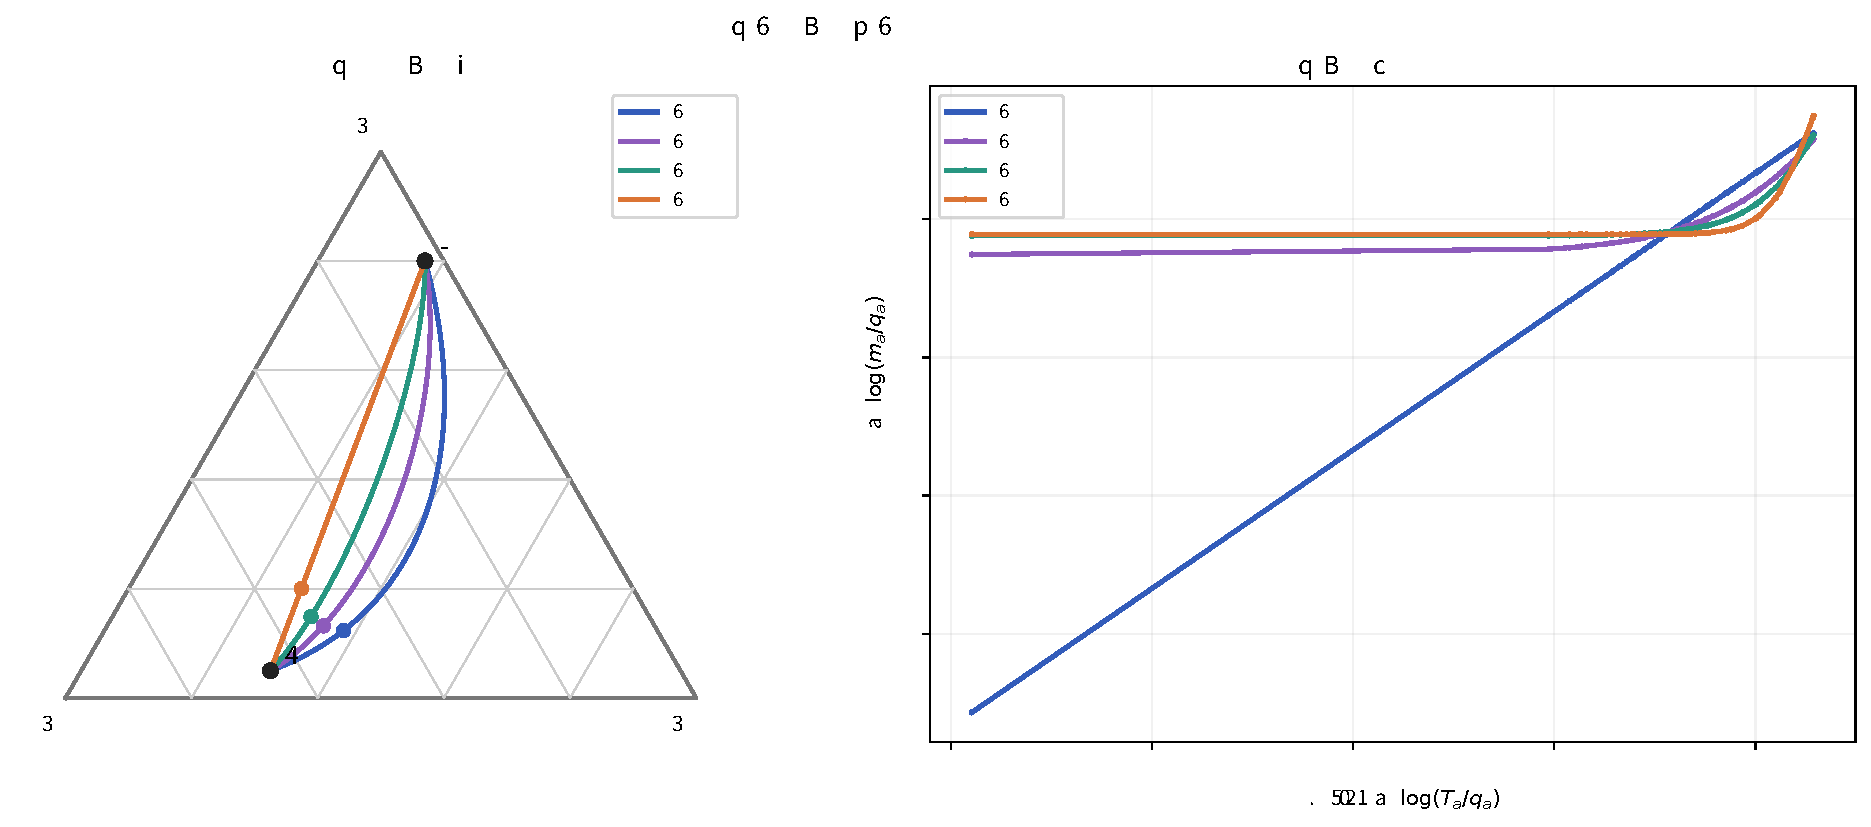
\includegraphics[width=\textwidth]{../../results/proximal-family-geometry/geometry.pdf}
 \caption{幂均值 target 的概率路径与 token log-ratio。左图圆点均为 $\eta=0.2$；右图以 64 维概率向量展示同一族。形状参数改变高维路径和尾部，而不是仅改变移动距离。}
\end{figure}
\subsection{重心唯一性与超额损失的精确分解}

散度 $D_\kappa$ 已由式~\eqref{eq:proximal-power-divergence} 定义。下面求解其加权重心，并把目标误差精确分解为到 target 的散度。

\begin{theorem}[幂均值重心与精确目标误差]
\label{thm:proximal-barycenter-gap}
对 $0<\kappa<1$，令
\begin{equation}
 F(p)=(1-\eta)D_\kappa(q\Vert p)+\eta D_\kappa(T\Vert p).
 \label{eq:proximal-divergence-barycenter}
\end{equation}
其唯一最小点是式~\eqref{eq:proximal-power-target} 的 $m$。对任意 $p$ 有
\begin{equation}
 F(p)=\frac{1-Z^\kappa}{\kappa(1-\kappa)}+Z^\kappa D_\kappa(m\Vert p),\qquad
 F(p)-F(m)=Z^\kappa D_\kappa(m\Vert p).
 \label{eq:proximal-gap-identity}
\end{equation}
端点 $\kappa=0,1$ 的超额损失分别为 $\KL(p\Vert m)$ 与 $\KL(m\Vert p)$。
\end{theorem}

\begin{proof}
令 $S_a=(1-\eta)q_a^\kappa+\eta T_a^\kappa$。目标写成 $F(p)=(1-\sum_aS_ap_a^{1-\kappa})/[\kappa(1-\kappa)]$。在 $\sum p_a=1$ 约束下，一阶条件为
\begin{equation}
 -\frac{S_a}{\kappa}p_a^{-\kappa}+\nu=0,
 \qquad p_a=(S_a/(\kappa\nu))^{1/\kappa}.
\end{equation}
归一化得到 $m$。目标的概率坐标 Hessian 为 $\operatorname{diag}(S_ap_a^{-\kappa-1})\succ0$，故内点解唯一。由 $S_a=Z^\kappa m_a^\kappa$，直接代入可得
\begin{align}
 F(p)
 &=\frac{1-Z^\kappa\sum_am_a^\kappa p_a^{1-\kappa}}{\kappa(1-\kappa)}\\
 &=\frac{1-Z^\kappa}{\kappa(1-\kappa)}
 +Z^\kappa\frac{1-\sum_am_a^\kappa p_a^{1-\kappa}}{\kappa(1-\kappa)}.
\end{align}
$p=m$ 时散度为零，得精确分解。$\kappa=0$ 时加权 reverse KL 展开为 $\KL(p\Vert m)-\log Z_0$；$\kappa=1$ 时加权 forward KL 展开为 $\KL(m\Vert p)+(1-\eta)\KL(q\Vert m)+\eta\KL(T\Vert m)$，其中 $Z_0=\sum q^{1-\eta}T^\eta$。端点的超额损失结论随之成立。\hfill$\square$
\end{proof}

定理把“相同 target”加强成了“原重心问题的超额损失与拟合散度精确成比例”。它也给出有限 inner 阶段适合验收的误差：若原问题优化误差为 $\delta$，则 $D_\kappa(m\Vert p)=\delta/Z^\kappa$。MDPO 使用的 $\KL(p\Vert m)$ 与它只有在 $\kappa=0$ 时完全相同；一般 $\kappa$ 下不能仅凭相同最小点替换有限步进展保证。
\subsection{共同的局部 Fisher 曲率与多教师扩展}

取 $p=u+\delta$、$\sum_a\delta_a=0$，并令 $\max_a|\delta_a/u_a|\to0$。逐项展开得到
\begin{equation}
 u_a^\kappa(u_a+\delta_a)^{1-\kappa}
 =u_a+(1-\kappa)\delta_a-\frac{\kappa(1-\kappa)}2\frac{\delta_a^2}{u_a}
 +O(|\delta_a|^3/u_a^2).
\end{equation}
求和后一次项消失，所以 $D_\kappa(u\Vert u+\delta)=\tfrac12\sum_a\delta_a^2/u_a+O(\sum_a|\delta_a|^3/u_a^2)$。在最优点 $m$，$S_am_a^{-\kappa-1}=Z^\kappa/m_a$。故对切向量 $v$、$\sum_av_a=0$，有
\begin{equation}
 \nabla_p^2F(m)[v,v]=Z^\kappa\sum_a\frac{v_a^2}{m_a}.
\end{equation}
若参数化模型恰好实现 $p_\theta=m$，令 $J_\theta=\partial p_\theta/\partial\theta$，则
\begin{equation}
 \nabla_\theta^2F(p_\theta)\big|_{p_\theta=m}
 =Z^\kappa J_\theta^\top\operatorname{diag}(1/m)J_\theta
 =Z^\kappa\mathcal I_\theta(m).
 \label{eq:proximal-fisher-hessian}
\end{equation}
推导中，$\nabla_pF(m)$ 是常数向量，其与 $\partial_\theta^2p_\theta$ 的乘积因 $\sum_ap_{\theta,a}=1$ 而消失。这个等式只在 target 可实现的最优点成立；远离最优点或有模型投影误差时，Hessian 一般还含额外项，不能宣称参数空间全局凸。

\begin{figure}[htbp]
 \centering
 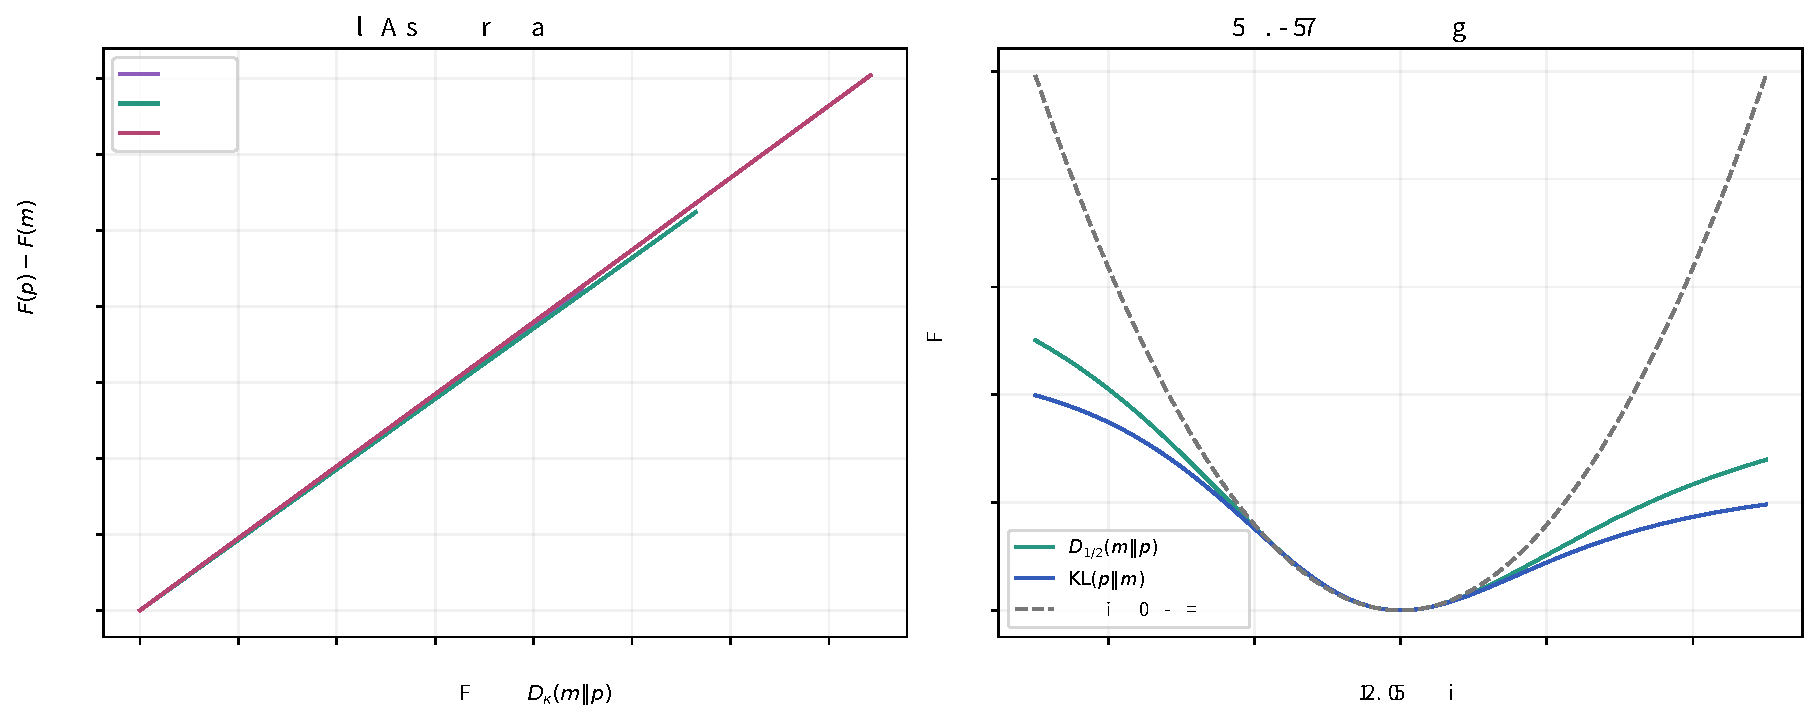
\includegraphics[width=\textwidth]{../../results/proximal-family-geometry/decomposition.pdf}
 \caption{左图检验 $F(p)-F(m)=Z^\kappa D_\kappa(m\Vert p)$，所有点位于对应常数斜率的直线上。右图固定同一个平方根 target，比较 Hellinger 与 reverse KL 拟合：共同的二阶曲率不消除远处损失的差异。}
\end{figure}

% END SOURCE: sections/proximal_barycenters.tex


\section{精确镜像下降的教师目标}

% BEGIN SOURCE: book/sections/proximal_md_objective.tex
\label{sec:proximal-md-objective}

幂均值重心定义了 target，但尚未指定对固定教师最小化什么函数。本节从冻结信号积分出一个不依赖 anchor 的教师目标，证明有限步幂均值恰为其标准熵镜像下降（Mirror Descent，MD）。固定 $\kappa,\eta$ 和教师时目标不变；改变 $\eta$ 会同时改变目标与原更新步长。

\subsection{由冻结信号反求生成函数}

\begin{theorem}[幂均值信号的可积性与精确 MD 目标]
\label{thm:power-md-integrable-objective}
记 $A=A_{\kappa,\eta}$，定义规范化生成函数
\begin{equation}
 \omega_{\kappa,\eta}(x)
 =x\int_1^x\frac{A_{\kappa,\eta}(u)}{u^2}\,du,
 \qquad x>0,
 \label{eq:power-md-generator-integral}
\end{equation}
以及教师目标
\begin{equation}
 \mathcal J_{\kappa,\eta}(p;T)
 =D_{\omega_{\kappa,\eta}}(T\Vert p)
 =\sum_a p_a\omega_{\kappa,\eta}(T_a/p_a).
 \label{eq:power-md-fixed-objective}
\end{equation}
则 $\omega(1)=\omega'(1)=0$、$\omega''(x)>0$，$\mathcal J\ge0$ 且唯一零点为 $p=T$。在正正交象限内，$\mathcal J$ 的坐标梯度恰为
\begin{equation}
 \frac{\partial\mathcal J}{\partial p_a}(p;T)
 =-A_{\kappa,\eta}(T_a/p_a).
 \label{eq:power-md-exact-gradient}
\end{equation}
因此步长 $\eta$ 的 entropy MD 更新
\begin{equation}
 p^+=\argmin_{p\in\Delta}
 \left\{\langle\nabla\mathcal J(q;T),p-q\rangle
       +\frac1\eta\KL(p\Vert q)\right\}
 \label{eq:power-md-exact-step}
\end{equation}
严格等于幂均值 target $m_{\kappa,\eta}$。
\end{theorem}

\begin{proof}
对积分定义求导，得到
\begin{align}
 \omega'(x)&=\int_1^x\frac{A(u)}{u^2}\,du+\frac{A(x)}x,\\
 \omega(x)-x\omega'(x)&=-A(x),\\
 \omega''(x)&=\frac{A'(x)}x
 =\frac{x^{\kappa-2}}{1-\eta+\eta x^\kappa}>0.
 \label{eq:power-md-curvature}
\end{align}
最后一个式子对 $\kappa=0$ 按连续端点取值为 $1/x^2$。$A(1)=0$ 保证两项规范化条件。严格凸性给出 $\omega\ge0$，Jensen 等号条件和分布归一化给出散度的唯一零点。逐项使用链式法则，令 $x=T_a/p_a$，则
\begin{equation}
 \frac\partial{\partial p_a}[p_a\omega(T_a/p_a)]
 =\omega(x)-x\omega'(x)=-A(x).
\end{equation}
这一步把固定 anchor 上的信号提升为一个对任意当前分布 $p$ 定义的目标梯度。将它代入 MD 子问题，再对 $\sum p=1$ 引入乘子 $\nu$，有
\begin{equation}
 -A(T_a/q_a)+\eta^{-1}[\log(p_a/q_a)+1]+\nu=0.
\end{equation}
归一化后 $p_a^+\propto q_a\exp[\eta A(T_a/q_a)]$，正是前文的幂均值 target。该子问题严格凸，解唯一。

反过来，若规范化生成函数满足 $\omega-x\omega'=-A$，则 $(\omega/x)'=A/x^2$，连同 $\omega(1)=0$ 唯一确定式~\eqref{eq:power-md-generator-integral}。因此所构造的规范化函数是这一逐坐标梯度对应的唯一生成函数。
\end{proof}

\subsection{单调概率比信号的通用 $f$ 散度框架}

\begin{proposition}[单调信号的可积性与相对光滑性]
\label{prop:power-general-signal-framework}
设 $S:(0,\infty)\to\mathbb R$ 连续可微，$S(1)=0$、$S'(x)>0$。定义
\begin{equation}
 \omega_S(x)=x\int_1^x\frac{S(u)}{u^2}\,du,\qquad
 \mathcal J_S(p;T)=D_{\omega_S}(T\Vert p).
\end{equation}
则 $\omega_S$ 严格凸、规范化，且 $\nabla_p\mathcal J_S=-S(T/p)$。对该目标执行步长 $\tau$ 的熵 MD，精确解为 $p^+\propto q\exp[\tau S(T/q)]$。若
\begin{equation}
 L_S=\sup_{x>0}xS'(x)<\infty,
\end{equation}
则 $\mathcal J_S$ 相对于负熵 $H$ 为 $L_S$ 相对光滑；$0<\tau\le1/L_S$ 时具有本节单步下降与三点进展的相应保证。
\end{proposition}

\begin{proof}
积分微分给出 $\omega_S-x\omega_S'=-S$、$\omega_S''=S'/x>0$ 及 $\omega_S(1)=\omega_S'(1)=0$。透视函数求导后得到 $\nabla_p\mathcal J_S=-S(T/p)$，MD 一阶条件与归一化给出所列解。再令 $x_a=T_a/p_a$，有
\begin{equation}
 \nabla_p^2\mathcal J_S
 =\operatorname{diag}[x_aS'(x_a)/p_a]
 \preceq L_S\operatorname{diag}(1/p_a)=L_S\nabla^2H.
\end{equation}
沿连接两个正分布的线段积分 Hessian，得到相对光滑不等式。本节下降与三点证明只使用这个 Hessian 界、目标凸性和 MD 一阶条件，将 $1/\eta$ 替换成 $L_S$ 后逐步成立。
\end{proof}

幂均值信号属于这个框架，因为 $xA'(x)=x^\kappa/(1-\eta+\eta x^\kappa)\le1/\eta$。其他单调信号也可定义不同的凸教师目标；第~\ref{cor:power-general-signal-all-f}~推论进一步证明所列步幅下的共同教师散度进展。统一尾部界、可估计中心和良好的 BPO 投影仍需分别证明，可积性本身不保证这些额外性质。

\subsection{幂散度、reverse KL 与归一化 JS 的关系}

\begin{theorem}[精确 MD 目标的端点与曲率插值]
\label{thm:power-md-objective-endpoints}
固定正支持分布时，
\begin{align}
 \mathcal J_{0,\eta}(p;T)&=\KL(p\Vert T),\\
 \lim_{\eta\to0}\mathcal J_{\kappa,\eta}(p;T)&=D_\kappa(T\Vert p),\\
 \lim_{\eta\to1}\mathcal J_{\kappa,\eta}(p;T)&=\KL(p\Vert T).
 \label{eq:power-md-objective-limits}
\end{align}
算术形状 $\kappa=1$ 的有限 $\eta$ 目标为
\begin{equation}
 \boxed{\mathcal J_{1,\eta}(p;T)
 =\frac{(1-\eta)\KL(p\Vert M)+\eta\KL(T\Vert M)}{\eta(1-\eta)},
 \quad M=(1-\eta)p+\eta T.}
 \label{eq:power-md-js-endpoint}
\end{equation}
分子是权重为 $(1-\eta,\eta)$ 的 Jensen--Shannon（JS）散度。对所有 $x>0$，生成函数的曲率满足
\begin{equation}
 \frac1{\omega_{\kappa,\eta}''(x)}
 =\frac{1-\eta}{g_\kappa''(x)}+\frac\eta{g_0''(x)}.
 \label{eq:power-md-harmonic-curvature}
\end{equation}
所以精确 MD 目标以曲率的加权调和平均连接幂散度与 reverse KL；它一般不同于两种散度的加权和。
\end{theorem}

\begin{proof}
$\kappa=0$ 时 $A=\log x$，积分直接得到 $\omega=x-1-\log x=g_0$。在任意固定有限积分区间，$\eta\to0$ 时 $A\to(x^\kappa-1)/\kappa$，$\eta\to1$ 时 $A\to\log x$，而分母在该区间内有统一正下界。故可交换积分与极限。小 $\eta$ 时的极限生成函数与 $g_\kappa$ 有相同的二阶导数 $x^{\kappa-2}$ 及相同规范化条件；两者相等。有限词表允许逐项取散度极限。

对 $\kappa=1$，记 $a=1-\eta$、$B=a+\eta x$。分部积分给出
\begin{align}
 \omega_{1,\eta}(x)
 &=-\eta^{-1}\log B+x\int_1^x\frac{du}{u(a+\eta u)}\\
 &=\frac{x\log x}{a}-\left(\frac1\eta+\frac xa\right)\log B
 =\frac{\eta x\log x-B\log B}{\eta a}.
\end{align}
代入 $x=T/p$ 得到
\begin{equation}
 \mathcal J_{1,\eta}(p;T)
 =\frac{\eta\KL(T\Vert p)-\KL(M\Vert p)}{\eta a}.
\end{equation}
展开两项 KL，使用 $M=ap+\eta T$，其分子等于 $a\KL(p\Vert M)+\eta\KL(T\Vert M)$，得到式~\eqref{eq:power-md-js-endpoint}。最后，式~\eqref{eq:power-md-curvature} 的倒数为 $a x^{2-\kappa}+\eta x^2$；两项分别是 $a/g_\kappa''$ 与 $\eta/g_0''$。
\end{proof}

因此涉及两个 KL 方向的准确表述是：重心散度 $D_\kappa$ 在 $\kappa=0,1$ 分别为 reverse/forward KL；精确 MD 目标 $\mathcal J_{\kappa,\eta}$ 在固定正 $\eta$ 下的 $\kappa=1$ 端点是归一化加权 JS，随后令 $\eta\to0$ 才恢复 forward KL。中心 $K_{1,\eta}$ 则是 reverse KL 到混合分布，属于第三个对象。

对固定 $\kappa>0$，两个不同的插值强度一般也不能仅用目标的整体缩放互相替代。若 $\omega_{\kappa,\eta_1}=b\omega_{\kappa,\eta_2}$，则一处的二阶导数均为一，强制 $b=1$；式~\eqref{eq:power-md-curvature} 随后要求 $1-\eta_1+\eta_1x^\kappa=1-\eta_2+\eta_2x^\kappa$ 对所有 $x$ 成立，只能有 $\eta_1=\eta_2$。因此 $\eta$ 是教师目标的形状选择，同时也是原幂均值更新的 MD 步长；若要在同一个 $\mathcal J$ 上单独调节 MD 步长，应固定 $\eta$，另用后文的 $\tau$。

\begin{center}
\small
\begin{tabular}{lll}
\toprule
散度及用途 & $\kappa=0$ & $\kappa=1$、固定 $0<\eta<1$\\
\midrule
$D_\kappa(T\Vert p)$：定义重心 & $\KL(p\Vert T)$ & $\KL(T\Vert p)$\\
$\mathcal J_{\kappa,\eta}(p;T)$：精确 MD 目标 & $\KL(p\Vert T)$ & $\mathrm{JS}_\eta(p,T)/[\eta(1-\eta)]$\\
$K_{\kappa,\eta}(q,T)$：冻结教师中心 & $\KL(q\Vert T)$ & $\KL(q\Vert(1-\eta)q+\eta T)/\eta$\\
\bottomrule
\end{tabular}
\end{center}

\begin{theorem}[精确 MD 目标的锐统一上界]
\label{thm:power-md-uniform-cap}
若 $0<\kappa\le1$、$0<\eta<1$，定义
\begin{equation}
 c=-\frac{\log(1-\eta)}{\kappa\eta},\qquad
 d=\int_1^\infty\frac{A_{\kappa,\eta}(u)}{u^2}\,du.
\end{equation}
则 $0<d\le1/\eta$，并有
\begin{equation}
 0\le\mathcal J_{\kappa,\eta}(p;T)\le c+d.
 \label{eq:power-md-uniform-cap}
\end{equation}
上界不依赖词表维数，并且在至少二元的完整支持分布类上是锐上确界。算术形状满足
\begin{equation}
 c+d=\frac{-\eta\log\eta-(1-\eta)\log(1-\eta)}{\eta(1-\eta)}.
\end{equation}
原始 reverse KL 的 $\kappa=0$ 端点没有有限统一上界。
\end{theorem}

\begin{proof}
当 $u\ge1$，$A(u)>0$（除 $u=1$ 外），且 $1-\eta+\eta u^\kappa\le u^\kappa$，所以 $A(u)\le\log u/\eta$。又有 $\int_1^\infty(\log u)/u^2\,du=1$，得到 $0<d\le1/\eta$。积分定义给出 $\omega(x)/x\to d$（$x\to\infty$）。当 $x\to0$ 时 $A(x)\to-c$，写成
\begin{equation}
 \omega(x)=-x\int_x^1\frac{A(u)}{u^2}\,du\longrightarrow c.
\end{equation}
要核实最后一个极限，可对任意 $\epsilon>0$ 选取足够小的 $b$，使 $|A(u)+c|\le\epsilon$ 对 $u\le b$ 成立；区间 $[b,1]$ 的积分乘以 $x$ 趋零，区间 $[x,b]$ 的误差不超过 $\epsilon x(1/x-1/b)\le\epsilon$。

凸函数的导数不超过其无穷远渐近斜率 $d$，从零处积分可得 $\omega(x)\le c+dx$。对 $x=T/p$ 求 $p$ 期望，得到 $\mathcal J\le c+d$。取 $p=(\epsilon,1-\epsilon)$、$T=(1-\epsilon,\epsilon)$，则稀有 $p$ 坐标的贡献趋于 $d$，另一坐标的贡献趋于 $c$，证明锐性。算术形状的显式生成函数给出 $d=-\log\eta/(1-\eta)$，与 $c$ 相加得到归一化二元熵。$\kappa=0$ 时 $\omega=g_0$ 在零处发散，前述锐界退化为无穷大。
\end{proof}
\subsection{全局相对光滑、单步下降与外层收敛率}

\begin{theorem}[精确幂均值 MD 的下降与收敛]
\label{thm:power-md-relative-smoothness}
固定教师、$\kappa,\eta$，令 $H(p)=\sum_ap_a\log p_a$。在正单纯形内，$\mathcal J=\mathcal J_{\kappa,\eta}$ 相对于 $H$ 具有常数 $1/\eta$ 的相对光滑性：对任意正分布 $p,q$，
\begin{equation}
 \mathcal J(p;T)\le\mathcal J(q;T)+\langle\nabla\mathcal J(q;T),p-q\rangle
       +\eta^{-1}\KL(p\Vert q).
 \label{eq:power-md-relative-smoothness}
\end{equation}
若 $p^+\propto q\exp[\tau A(T/q)]$、$0<\tau\le\eta$，则
\begin{align}
 \mathcal J(q;T)-\mathcal J(p^+;T)
 &\ge\tau^{-1}\KL(q\Vert p^+)
  +(\tau^{-1}-\eta^{-1})\KL(p^+\Vert q),\\
 \tau\mathcal J(p^+;T)
 &\le\KL(T\Vert q)-\KL(T\Vert p^+).
 \label{eq:power-md-single-step-progress}
\end{align}
对每步刷新 anchor 的精确迭代 $q_{n+1}=p^+(q_n)$、步长 $0<\tau_n\le\eta$，有
\begin{equation}
 \mathcal J(q_N;T)\le
 \frac{\KL(T\Vert q_0)}{\sum_{n=0}^{N-1}\tau_n}.
 \label{eq:power-md-last-iterate-rate}
\end{equation}
特别地，$\tau_n=\eta$ 时每步就是幂均值 target，最后迭代误差不超过 $\KL(T\Vert q_0)/(\eta N)$。
\end{theorem}

\begin{proof}
记 $x_a=T_a/p_a$。根据式~\eqref{eq:power-md-exact-gradient}，目标在正正交象限的 Hessian 为
\begin{equation}
 \nabla_p^2\mathcal J(p;T)
 =\operatorname{diag}\left(\frac1{p_a}
       \frac{x_a^\kappa}{1-\eta+\eta x_a^\kappa}\right)
 \preceq\eta^{-1}\operatorname{diag}(1/p_a)
 =\eta^{-1}\nabla^2H(p).
 \label{eq:power-md-hessian-bound}
\end{equation}
对连接 $q,p$ 的线段积分二阶 Taylor 余项，得到相对光滑不等式。目标本身严格凸，其 Hessian 的每个对角元为正。

设 $g=\nabla\mathcal J(q;T)$。MD 的一阶条件给出 $g_a+\tau^{-1}\log(p_a^+/q_a)$ 为常数。与 $p^+-q$ 内积时常数消失，故
\begin{equation}
 \langle g,p^+-q\rangle
 =-\tau^{-1}[\KL(p^+\Vert q)+\KL(q\Vert p^+)].
\end{equation}
代入相对光滑式，得到第一个下降界。再用凸性 $\mathcal J(q;T)-\mathcal J(T;T)\le\langle g,q-T\rangle$，以及 $\mathcal J(T;T)=0$，得到
\begin{align}
 \mathcal J(p^+;T)
 &\le\langle g,p^+-T\rangle+\eta^{-1}\KL(p^+\Vert q)\\
 &=\tau^{-1}[\KL(T\Vert q)-\KL(T\Vert p^+)]
   -(\tau^{-1}-\eta^{-1})\KL(p^+\Vert q)\\
 &\le\tau^{-1}[\KL(T\Vert q)-\KL(T\Vert p^+)].
\end{align}
第二行使用熵 Bregman 的三点恒等式，可直接展开各 KL 核验。对 $n=0,\ldots,N-1$ 求和，非负的末项 KL 给出
\begin{equation}
 \sum_{n=0}^{N-1}\tau_n\mathcal J(q_{n+1};T)\le\KL(T\Vert q_0).
\end{equation}
由第一个下降界，$\mathcal J(q_N;T)\le\mathcal J(q_{n+1};T)$，故左侧至少为 $(\sum\tau_n)\mathcal J(q_N;T)$，得到最后迭代界。
\end{proof}

这个定理无需概率统一正下界，只要求给定有限分布严格为正；初始 $\KL(T\Vert q_0)$ 可以很大。若 $\sum\tau_n\to\infty$，则 $\mathcal J(q_N;T)\to0$，严格凸散度及有限单纯形紧性保证 $q_N\to T$。边界也不能形成额外的零点：由积分定义，
\begin{equation}
 \lim_{x\to\infty}\frac{\omega(x)}x
 =\int_1^\infty\frac{A(u)}{u^2}\,du=:d_\infty>0.
\end{equation}
该积分有限，因为 $0\le A(u)\le\log u/\eta$ 对 $u\ge1$ 成立。若某个坐标 $p_a\to0$，则 $p_a\omega(T_a/p_a)\to T_a d_\infty>0$。任何内点极限的零损失又强制各比率都等于一。因此所有收敛子列的极限只能是 $T$，整个序列收敛到 $T$。

对固定 anchor 的 BPO 内层，理想路径 $p_\xi\propto q\exp[\xi\eta A(T/q)]$、$0\le\xi\le1$ 对应从该 anchor 做一步步长为 $\tau=\xi\eta$ 的上述 MD；因而具有同一单步界。这里的外层收敛率要求每步重新计算信号并刷新 anchor。实际共享参数 BPO/AdamW 只有近似投影时，需要另外控制拟合误差；任意 BPO loss 下降不能自动套用该定理。若外层改变 $\eta$ 或 $\kappa$，目标 $\mathcal J$ 也改变，不能把各步的不等式直接望远镜求和。

% END SOURCE: sections/proximal_md_objective.tex


% BEGIN SOURCE: book/sections/proximal_md_variants.tex
\subsection{保留 KL 子问题与保留原教师目标的 MD 有别}

标准 entropy MD 对一个固定目标 $F$ 执行
\begin{equation}
 p^+=\argmin_p\{\langle\nabla F(q),p-q\rangle+\eta^{-1}\KL(p\Vert q)\}.
\end{equation}
取 $F_0(p)=\KL(p\Vert T)$，有 $\nabla F_0(q)=\log(q/T)+1$，与 $-r$ 只差常数，因而 $\kappa=0$ 的几何目标就是对原 reverse KL 的标准 entropy MD。

若 $\kappa>0$，有效梯度为 $-A_{\kappa,\eta}$，它本身依赖 $\eta$。其导数对 $r$ 为
\begin{equation}
 \frac{d}{dr}A_{\kappa,\eta}(e^r)=\frac{e^{\kappa r}}{1-\eta+\eta e^{\kappa r}}.
\end{equation}
当 $0<\eta<1$ 时它不是恒等于一的常数，所以一般不能用一个标量重新设定步长恢复原来的 $-r$ 方向。式~\eqref{eq:power-bpo-mirror-subproblem} 是精确的 entropy mirror 子问题，但不能称为对原 $F_0$ 的同一个 MD 更新。$\eta=1$ 或 $q=T$ 是特殊退化情况。信号依赖 $\eta$ 不妨碍为每个固定 $(\kappa,\eta)$ 构造另一个不依赖 anchor 的目标；本节已经给出新目标 $\mathcal J$ 的生成函数及收敛证明。

\subsection{连续极限是 teacher 散度的自然梯度流}

对 $\eta\to0$，记 $\rho_a=T_a/q_a$、$a_\kappa=\E_q\rho^\kappa$。逐项展开 $h_a=q_a[1+\eta(\rho_a^\kappa-1)/\kappa+O(\eta^2)]$ 并归一化，得到
\begin{equation}
 m_a=q_a+\eta v_{\kappa,a}+O(\eta^2),\qquad
 v_{\kappa,a}=\frac{q_a}{\kappa}(\rho_a^\kappa-a_\kappa).
 \label{eq:proximal-natural-velocity}
\end{equation}
展开针对固定完整支持的 $q,T$；其余项不能在任意极端概率比上直接视为统一 $O(\eta^2)$。$\kappa=0$ 的极限为 $v_{0,a}=q_a[\log\rho_a-\E_q\log\rho]$，$\kappa=1$ 为 $v_1=T-q$。

概率单纯形的 Fisher 度量为 $\langle v,w\rangle_q=\sum_av_aw_a/q_a$。若 $g_a$ 是 $L$ 的概率梯度代表，则负自然梯度为 $-q_a(g_a-\E_qg)$：其分量和为零，且对任何切向量 $w$，Fisher 内积恰好等于 $-\sum_ag_aw_a$。取 $L(q)=D_\kappa(T\Vert q)$，可取 $g_a=-\rho_a^\kappa/\kappa$；规范化生成函数给出的代表为 $(1-\rho_a^\kappa)/\kappa$，相差的常数被中心化消掉。因此 $v_\kappa=-\operatorname{grad}_{\!F}D_\kappa(T\Vert q)$。连续时间 $t$ 下
\begin{equation}
 \frac{dq_a}{dt}=v_{\kappa,a},\qquad
 \frac{d}{dt}D_\kappa(T\Vert q)
 =-\|v_\kappa\|_F^2
 =-\frac1{\kappa^2}\Var_q(\rho^\kappa).
 \label{eq:proximal-flow-lyapunov}
\end{equation}
最后一步由 $\sum_av_a=0$ 及 $g^\top v=-(\E_q\rho^{2\kappa}-a_\kappa^2)/\kappa^2$ 得到。$\kappa=0$ 时右侧为 $-\Var_q(\log\rho)$。所有形状参数都对应同一 Fisher 度量，但所下降的全局 teacher 散度不同。
\subsection{对固定幂散度执行有限步 MD 的另一种更新}

若要求在有限步长下严格采用这个固定 $F_\kappa$ 的 entropy MD，应另取
\begin{equation}
 \widetilde m_a\propto q_a
   \exp\left(\tau\frac{(T_a/q_a)^\kappa-1}{\kappa}\right).
 \label{eq:power-bpo-true-md-variant}
\end{equation}
它与幂均值目标只有一阶一致，有限 $\tau$ 时一般不同；并且指数中的概率比幂会重新引入极端正信号。另一种解释是第~\ref{sec:power-projection}~节 escort 坐标中的自适应二次目标梯度步，但这改变了坐标和目标，不应据此给实际神经网络 inner 更新贴上标准 MD 标签。

直接把 $D_\kappa(q\Vert p)$ 当成原负熵的 Bregman 正则也不正确：对 $0<\kappa<1$，它对 $p$ 的 Hessian 为 $\operatorname{diag}(q_a^\kappa p_a^{-\kappa-1})$，依赖参照 $q$。固定 mirror 势的 $B_\Phi(p,q)$ 对第一自变量的 Hessian 是 $\nabla^2\Phi(p)$，不依赖 $q$。一般情况下，两者不是同一 Bregman 散度。

% END SOURCE: sections/proximal_md_variants.tex


\section{单 rollout 的 BPO 算法与内层拟合}

% BEGIN SOURCE: book/sections/proximal_bpo_algorithm.tex
\label{sec:power-bpo-algorithm}

本节在第~\ref{sec:power-setup}~节定义的单教师、单 rollout 和冻结前缀测度上拟合 target。外层锚点 $q_n$ 与教师信号冻结，内层学生 $p_{n,j}$ 及其条件中心随参数更新。所有微分均不穿过 rollout、前缀权重、锚点与教师。

\subsection{形状参数只进入冻结监督信号}

使用式~\eqref{eq:proximal-power-signal} 与式~\eqref{eq:center-explicit-definition} 的冻结 $f,A$。目标构造已经由前两节证明，下面将它接到 BPO 的条件回归目标。

从下面的 KL mirror 子问题开始：
\begin{equation}
 m=\argmax_{p\in\Delta}
 \left\{\sum_a p_a A_{\kappa,\eta}(a)
       -\frac1\eta\KL(p\Vert q)\right\}.
 \label{eq:power-bpo-mirror-subproblem}
\end{equation}
根据第~\ref{thm:power-md-integrable-objective}~定理，其唯一解为
\begin{equation}
 m_a=q_ae^{f_a}/Z,\qquad Z=\sum_bq_be^{f_b}.
 \label{eq:power-bpo-explicit-target}
\end{equation}
改变 $\kappa$ 改变冻结监督和 target；KL 正则仍为 $\KL(p\Vert q)$。BPO 内层拟合这个 target，通常不直接最小化重心目标 $F$ 或教师目标 $\mathcal J$。

\subsection{BPO 损失、中心和精确梯度}

令 $C_qh=h-\E_qh$，定义
\begin{align}
 b_\theta&=\E_q[U_\theta-f],\\
 R_\theta(a)&=U_\theta(a)-f_a-b_\theta
            =C_q\log(p_\theta/m)_a,\\
 \mathcal L_n(\theta)
 &=\E_{s\sim\widehat d_n}\frac1{2\eta}
     \E_{a\sim q_n(\cdot\mid s)}R_\theta(s,a)^2.
 \label{eq:power-bpo-population-loss}
\end{align}
等价地，令 $\delta=C_q[U_\theta/\eta-A]$，则 $\mathcal L_n=(\eta/2)\E_{\widehat d_n,q}\delta^2$。$\kappa=0$ 时正好恢复原 BPO 的归一化损失。$\log Z$ 被 $C_q$ 消掉，因此无需显式计算 target 的归一化常数。teacher 监督只需本轮缓存 $f$ 及 $\E_qf$；学生项 $\E_qU_\theta$ 必须随 inner 参数更新，不能连同 teacher 中心一起冻结。

对固定 prefix，$\psi_\theta(a)=\nabla_\theta\log p_\theta(a)$。由于 $\nabla b_\theta=\E_q\psi_\theta$ 与 $\E_qR_\theta=0$，直接微分得到
\begin{align}
 \nabla_\theta\mathcal L_s
 &=\frac1\eta\E_q[R_\theta(\psi_\theta-\E_q\psi_\theta)]\\
 &=\frac1\eta\E_q[R_\theta\psi_\theta].
 \label{eq:power-bpo-gradient}
\end{align}
所以精确 BPO 不带 $p/q$ 重要性比率；测度就是冻结 $q$。若使用随机 action 估计最后一个期望，系数 $\sg(R_\theta/\eta)$ 乘以 $\log p_\theta(a)$ 给出所需 score 梯度。若直接微分完整平方损失，中心可以正常参与自动微分，其导数因精确零均值而抵消；两种停止梯度语义不能混为一谈。

用已定义的冻结中心 $K$ 展开 BPO 系数，得到
\begin{equation}
 \frac{R(a)}\eta
 =\frac{U(a)+\KL(q\Vert p)}\eta-A_{\kappa,\eta}(a)-K_{\kappa,\eta}.
\end{equation}
因此需要同时替换 action 监督 $r\mapsto A$ 和冻结教师中心 $\KL(q\Vert T)\mapsto K_{\kappa,\eta}$；只改变 action 监督却沿用原教师中心会产生偏差。$\kappa=0$ 时 $K_{0,\eta}=\KL(q\Vert T)$，恢复原接口。一般 $\kappa$ 下，由 $\E_qf=-\KL(q\Vert m)+\log Z$，有 $K_{\kappa,\eta}=[\KL(q\Vert m)-\log Z]/\eta$，它不是原 teacher KL。学生中心仍是当轮不断重算的 $\KL(q\Vert p)$。

完整支持下 $\mathcal L_s=0$ 当且仅当 $\log(p_a/m_a)$ 对全部 action 是常数。归一化强制该常数为零，因此 $p=m$。多 prefix、共享参数时，零损失还要求网络能同时表示全部条件 target；不可实现时只是 BPO 投影，不能宣称等于理想 mirror 更新。
\subsection{完整词表求和与一条轨迹的 action 估计}

一条 rollout 足以给出训练前缀，并不要求损失只使用每个前缀实际生成的一个 token。若能访问该前缀完整 $q,T,p$ 概率，可以直接求式~\eqref{eq:power-bpo-population-loss} 的 action 期望，仍然只有一次 response 生成，没有辅助 rollout 或候选组。这是本节的精确参考算法。

若只使用 rollout 中的 action，估计量为 $g(a)=R_\theta(a)\psi_\theta(a)/\eta$。对固定的 $s,\theta$ 和独立 $a\sim q(\cdot\mid s)$，它无偏。只用这一 action 同时估计本前缀的中心会令 $R=0$，使算法退化；把一条 response 的不同前缀 token 当作同一条件分布的组均值，也不能得到 $\E_{q(\cdot\mid s)}$。

复用整条已采样轨迹做 $I>1$ 个 inner 更新时，当前 $\theta$ 依赖已见 action，因而不再自动具有上述条件无偏性。给定固定样本 $a$，其平方残差损失的真正梯度是
\begin{equation}
 \nabla_\theta\frac{R_\theta(a)^2}{2\eta}
 =\frac{R_\theta(a)}\eta(\psi_\theta(a)-\E_q\psi_\theta),
\end{equation}
一般不等于停止系数的 $R_\theta(a)\psi_\theta(a)/\eta$。后者仍可作为 BPO population-gradient 的采样近似，但必须记录样本复用误差。对完整 rollout 的无偏性论证，还需 action 权重在抽取该 action 之前可确定；使用随机最终长度作分母是比率估计，不能直接套用逐条件无偏公式。完整词表求和对已冻结的经验前缀测度给出精确梯度，不受这些 action 估计问题影响。
\subsection{BPO 是带冻结测度的拟合损失}

对冻结 $q,m$，BPO population 损失是
\begin{equation}
 \mathcal L_{\mathrm{BPO}}(p;m,q)
 =\frac1{2\eta}\Var_q\!\left[\log\frac p m\right].
 \label{eq:divergence-map-bpo-loss}
\end{equation}
它一般不能写成仅以 $(p,m)$ 为自变量的 $D_g(p\Vert m)$。取二元词表，固定 $p,m$ 且 $\ell_1=\log(p_1/m_1)\ne\ell_2=\log(p_2/m_2)$，则
\begin{equation}
 \mathcal L_{\mathrm{BPO}}=\frac{q_1(1-q_1)}{2\eta}(\ell_1-\ell_2)^2.
\end{equation}
改变第三个分布 $q$ 会改变损失，任何固定生成函数的 $D_g(p\Vert m)$ 都不随 $q$ 改变。完整支持下，BPO 与 target 散度共享唯一零点 $p=m$，这一事实不意味着损失、曲率或有限步轨迹相同。

取切向扰动 $p=m+v$、$\sum_av_a=0$，并令全部 $v_a/m_a$ 一致趋零。展开 $\log(1+v_a/m_a)$ 得到
\begin{equation}
 \mathcal L_{\mathrm{BPO}}(m+v;m,q)
 =\frac1{2\eta}\left\{\sum_aq_a\frac{v_a^2}{m_a^2}
 -\left(\sum_aq_a\frac{v_a}{m_a}\right)^2\right\}
 +O\!\left(\max_a|v_a/m_a|^3\right).
\end{equation}
若 $q=m$，一次均值为 $\sum v=0$，二阶项恢复 $\sum v_a^2/m_a$ 的 Fisher 度量，另带 $1/\eta$。一般冻结 $q\ne m$ 时，BPO 的局部度量与 target 上的 Fisher 度量不同。若使用独立 logits $z$，则 $C_q\log(p/m)=C_q(z-\log m)$，全局 Hessian 为 $[\operatorname{diag}(q)-qq^\top]/\eta$，与 $\kappa$ 无关。

\subsection{BPO 的固定几何与有限 inner 性质}

令独立 logits 为 $z$，$p=\operatorname{softmax}(z)$。由于 $C_q$ 消掉 softmax 的归一化常数，单 prefix 损失成为
\begin{align}
 \mathcal L_s(z)&=\frac1{2\eta}
    (z-\log m)^\top Q_q(z-\log m),\\
 Q_q&=\operatorname{diag}(q)-qq^\top,\qquad
 \nabla_z\mathcal L_s=Q_q(z-\log m)/\eta,\\
 \nabla_z^2\mathcal L_s&=Q_q/\eta.
\end{align}
$Q_q$ 在常数方向为零，在 $\boldsymbol1^\perp$ 上正定。对 $v\perp\boldsymbol1$，
\begin{equation}
 v^\top Q_qv=\sum_aq_a(v_a-\E_qv)^2
 \ge q_{\min}\sum_a(v_a-\E_qv)^2
 \ge q_{\min}\|v\|^2.
\end{equation}
Gershgorin 界给出 $\lambda_{\max}(Q_q)\le\max_a2q_a(1-q_a)\le1/2$。独立 logits 的普通梯度下降因此在 $0<\alpha_{\mathrm{opt}}<2\eta/\lambda_{\max}(Q_q)$ 下收敛；$\alpha_{\mathrm{opt}}<4\eta$ 是充分条件。若 $h=z-\log m$ 的第 $i$ 个非零特征方向系数为 $c_i$，则
\begin{equation}
 \mathcal L_s(z_j)=\frac1{2\eta}\sum_i\lambda_i c_i^2
    (1-\alpha_{\mathrm{opt}}\lambda_i/\eta)^{2j}.
\end{equation}
这些是独立 logits 的精确结论，不是 AdamW 或共享神经网络的无条件收敛定理。固定 $q,\eta$ 时 $\kappa$ 完全不出现在 Hessian 中：它改变回归目标与起始残差，不改善这个二次问题的条件数。小 $\eta$ 会增大曲率，并不自动降低归一化后的起始梯度。

若 $\|\psi_\theta(a)\|\le S$，随机 action 梯度有
\begin{equation}
 \E_q\|g\|^2\le\frac{2S^2}{\eta}\mathcal L_s.
\end{equation}
在 $p=q$ 时 $R=-C_qf$，故 $\mathcal L_s(q)=\Var_q(f)/(2\eta)$。在可实现的 $p=m$ 处，每个 action 的残差和随机梯度都为零。因而 target 形状影响初始监督尾部，而 BPO 拟合本身提供残差下降时的噪声控制；两者承担不同作用。

BPO 损失下降并不自动意味着 teacher KL 或 $D_\kappa$ 下降。一个三元反例取 $q=(0.4999995,0.4999995,10^{-6})$、$T=(0.8,0.199999,10^{-6})$、$\eta=0.3$、$\kappa=0.5$。令 $p\propto m\exp(0,0,12)$。稀有 action 的 logit 误差由很小的 $q$ 权重计价，BPO 损失低于起点，却会显著提高 $\KL(p\Vert T)$。本节核验程序给出 $\mathcal L_s(q)=0.06227708$、$\mathcal L_s(p)=0.00024000$，而 $\KL(q\Vert T)=0.22314483$、$\KL(p\Vert T)=1.65421904$。因此有限 inner 仍需真 teacher 散度和拟合误差证书。

若在该 prefix 上控制 $\|R\|_\infty\le\epsilon$，记 $\ell=\log(p/m)=R+c$。由概率归一化 $c=-\log\E_me^R\in[-\epsilon,\epsilon]$，得到 $\|\ell\|_\infty\le2\epsilon$ 和 $\KL(p\Vert m)\le2\epsilon$。仅从 BPO 损失可保证 $\|R\|_\infty\le\sqrt{2\eta\mathcal L_s/q_{\min}}$，可以取这个上界为 $\epsilon$；大词表极小的 $q_{\min}$ 会使该保证很弱。这解释了精确最优点一致与有限拟合质量之间的差距。
\subsection{锚点 Fisher 预条件的 BPO 保留有限步镜像性质}

前面的反例允许任意候选 $p$。如果约束 inner 的实际路径，可以得到比零误差最优点更强的保证。仍使用独立 logits，令 $Q_q^+$ 为 $Q_q$ 的 Moore--Penrose 逆，采用冻结锚点 Fisher 预条件更新
\begin{align}
 z^+&=z-\gamma\eta Q_q^+\nabla_z\mathcal L_s
     =z-\gamma Q_q^+Q_q(z-\log m),\\
 p^+_a&\propto p_a^{1-\gamma}m_a^\gamma,\qquad 0<\gamma\le1.
 \label{eq:power-bpo-anchor-fisher-step}
\end{align}
由于 $Q_q^+Q_q$ 是 $\boldsymbol1^\perp$ 上的正交投影，它与恒等映射只差常数 logit；softmax 消掉该常数。因此上式是精确的分布恒等式。$Q_q$ 是锚点 $q$ 的 Fisher，不能改称当前 $p$ 的 Fisher。该更新也恰好等于以当前 $p$ 为 KL 正则参照、步幅 $\gamma$ 对固定拟合目标 $\KL(p\Vert m)$ 执行 entropy MD。这里的 KL 目标是本轮 $m$，不等于原教师目标 $T$。

从 $p_0=q$ 出发，允许每次 $0<\gamma_j\le1$，归纳得到
\begin{align}
 p_j&=p_{\xi_j},\qquad
 p_{\xi,a}=q_ae^{\xi f_a}/Z_\xi,\\
 \xi_j&=1-\prod_{h<j}(1-\gamma_h),\qquad
 \mathcal L_s(p_j)=(1-\xi_j)^2\mathcal L_s(q).
 \label{eq:power-bpo-finite-inner-path}
\end{align}
证明只需代入 $\log(p_\xi/q)=\xi f-\log Z_\xi$，于是 $R_\xi=-(1-\xi)C_qf$；再对几何插值的 log 密度求线性组合，得到 $\xi^+=\xi+\gamma(1-\xi)$。这个理想 inner 的损失收缩因子不依赖 $q_{\min}$ 或词表大小，因为预条件器消掉了 $Q_q$ 的非零谱；实际计算与神经网络可实现性另有成本。

\begin{theorem}[幂均值 BPO 镜像拟合路径的有限步 teacher 进展]
\label{thm:power-bpo-inner-all-f}
在完整正支持、$\kappa\in[0,1]$、$0<\eta\le1$ 下，对任意凸函数 $\Phi$、$\Phi(1)=0$，令
\begin{equation}
 D_\Phi(p\Vert T)=\sum_aT_a\Phi(p_a/T_a).
\end{equation}
沿 $p_\xi\propto qe^{\xi f}$、$0\le\xi\le1$，$D_\Phi(p_\xi\Vert T)$ 不增加。因而式~\eqref{eq:power-bpo-anchor-fisher-step} 从 $q$ 出发时，每个有限 inner 都不增加 teacher 双向 KL、总变差或平方 Hellinger 距离。
\end{theorem}

\begin{proof}
记 $r_a=\log(T_a/q_a)$。$f(r)$ 单调递增；当 $\kappa>0$ 时 $f'(r)=\eta e^{\kappa r}/(1-\eta+\eta e^{\kappa r})\le1$，$\kappa=0$ 时 $f'=\eta\le1$。于是
\begin{equation}
 u_{\xi,a}=\frac{p_{\xi,a}}{T_a}
 =\frac{\exp[-r_a+\xi f(r_a)]}{Z_\xi}
\end{equation}
作为 $r_a$ 的函数单调不增，因为 $-1+\xi f'(r)\le0$。对于可微凸 $\Phi$，$\Phi'(u)$ 随 $u$ 单调不减，所以 $\Phi'(u_\xi(r))$ 随 $r$ 单调不增。微分归一化密度给出 $\partial_\xi p_\xi=p_\xi(f-\E_{p_\xi}f)$，因此
\begin{align}
 \frac{d}{d\xi}D_\Phi(p_\xi\Vert T)
 &=\operatorname{Cov}_{p_\xi}(\Phi'(u_\xi),f)\\
 &=\frac12\sum_{a,b}p_{\xi,a}p_{\xi,b}
   [\Phi'(u_{\xi,a})-\Phi'(u_{\xi,b})](f_a-f_b)
 \le0.
\end{align}
每个乘积非正，因为两因子对 $r$ 的单调性相反。有限词表和完整正支持下，$\{u_{\xi,a}:\xi\in[0,1],a\in\mathcal V\}$ 位于一个紧的正区间。任意有限凸函数都可在该区间由光滑凸函数一致逼近，逐点极限保留上述非增加关系，得到不可微情形。取 $\Phi(u)=u\log u$、$-\log u$、$|u-1|/2$ 与 $(\sqrt u-1)^2$，分别给出双向 KL、总变差与平方 Hellinger。\hfill$\square$
\end{proof}

对固定前缀测度逐条件求加权和保留该保证。任意降低 BPO 损失的候选则没有这项性质。共享神经网络、随机梯度、Fisher 近似和前缀测度刷新都可能离开指定路径，需要分别控制误差。

\begin{corollary}[通用单调信号 MD 的共同教师散度进展]
\label{cor:power-general-signal-all-f}
采用第~\ref{prop:power-general-signal-framework}~命题的 $S$，设 $L_S<\infty$、$0<\tau\le1/L_S$。则沿
\begin{equation}
 p_\xi\propto q\exp[\xi\tau S(T/q)],\qquad0\le\xi\le1,
\end{equation}
任意凸 $f$ 散度 $D_\Phi(p_\xi\Vert T)$ 都非增加。因此该步幅条件既保证对应教师目标 $\mathcal J_S$ 的 MD 下降，也保证其他凸生成教师散度不增加。
\end{corollary}

\begin{proof}
记 $r=\log(T/q)$、$f(r)=\tau S(e^r)$。则 $f'(r)=\tau e^rS'(e^r)\in(0,1]$。前一定理的证明仅使用 $f$ 单调递增和 $f'\le1$，未在协方差非正的论证中使用幂均值的其他性质，故逐步适用于此处的 $f$。
\end{proof}

\begin{figure}[htbp]
 \centering
 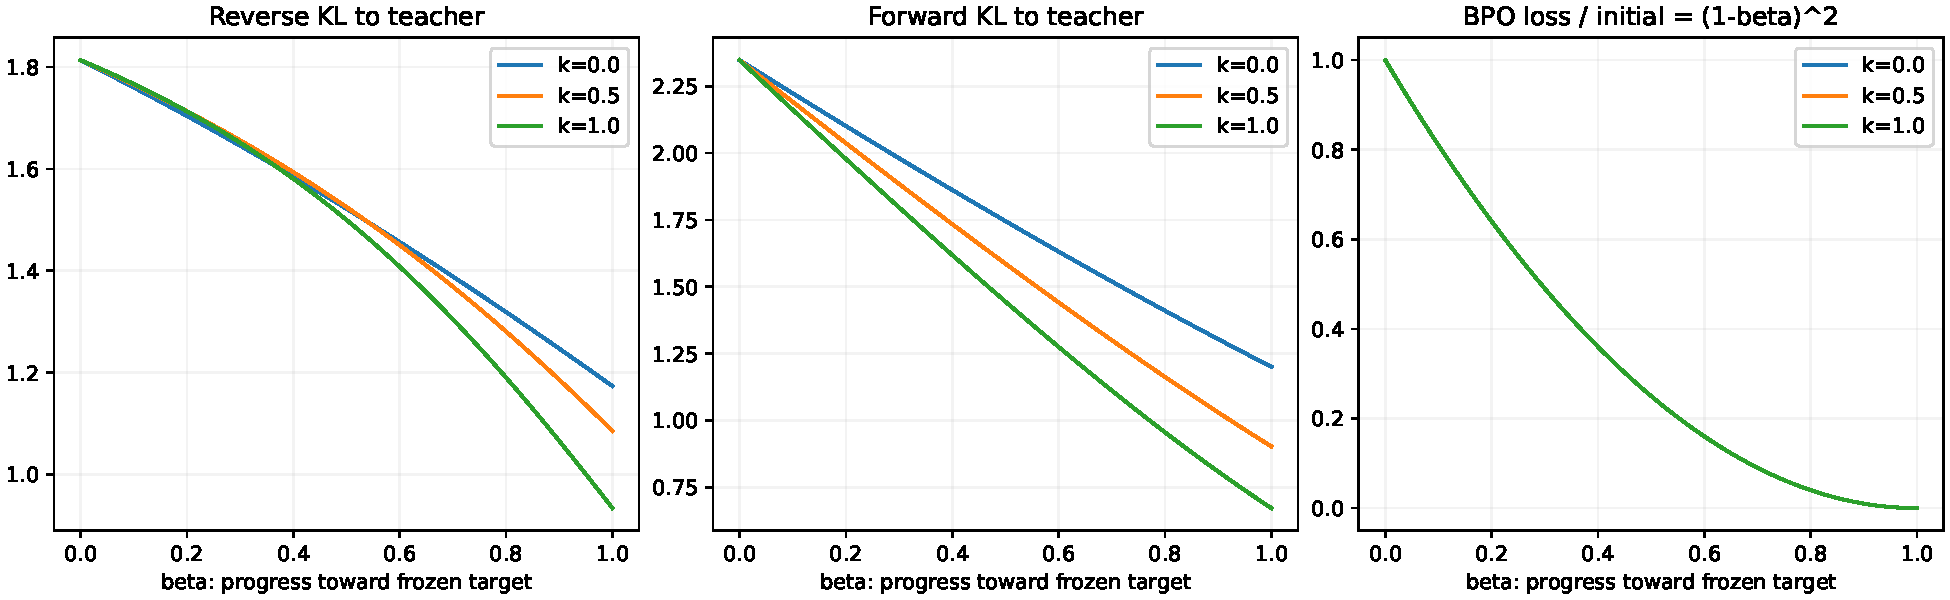
\includegraphics[width=\textwidth]{../../results/power-bpo-algorithm/finite-inner-progress.pdf}
 \caption{理想锚点 Fisher 预条件 BPO 的有限 inner：双向 teacher KL 沿 $\xi$ 下降，BPO 损失按 $(1-\xi)^2$ 精确收缩。图中旧记号 $\beta$ 对应本章 $\xi$；曲线为三元完整支持分布的解析求和。}
\end{figure}
\subsection{精确参考算法与实际 outer 更新}

\begin{algorithm}[htbp]
\caption{单 rollout 的幂均值 BPO\\{\small\textit{Semantics: 根据正文重构；完整词表条件期望}}}
\begin{algorithmic}[1]
\Require 教师 $T$，初始参数 $\theta_0$，prompt 测度 $\mathcal D$，batch 大小 $B\ge1$
\Require $0<\eta\le1$，$0\le\kappa\le1$，outer 预算 $N\ge1$，inner 次数 $I\ge1$
\For{outer $n=0,\ldots,N-1$}
    \State $q_n\gets\sg(\pi_{\theta_n})$
    \State $x_1,\ldots,x_B\overset{\mathrm{iid}}\sim\mathcal D$
    \For{每个 prompt 槽位 $x_i$}
        \State $y_i\sim q_n(\cdot\mid x_i)$ \Comment{恰好一条 rollout}
        \State 冻结其有效前缀与权重；若无有效前缀，跳过该槽位
        \For{每个有效前缀 $s$}
            \State 缓存 $q_n(\cdot\mid s)$，$f_s\gets\sg(f_{\kappa,\eta}(\log(T/q_n)))$，$\bar f_s\gets\E_{q_n}f_s$
        \EndFor
    \EndFor
    \If{所有槽位均无有效前缀}
        \State $\theta_{n+1}\gets\theta_n$
        \State 跳过本轮更新，重新采样下一批 prompt
    \Else
        \State $\theta_{n,0}\gets\theta_n$
        \For{$j=0,\ldots,I-1$}
            \State $U_{s,a}\gets\log(\pi_{\theta_{n,j}}(a\mid s)/q_n(a\mid s))$
            \State $R_{s,a}\gets U_{s,a}-f_{s,a}-\E_{q_n}(U_s-f_s)$
            \State $\mathcal L\gets\sum_sw_s\sum_aq_n(a\mid s)R_{s,a}^2/(2\eta)$
            \State $\theta_{n,j+1}\gets\theta_{n,j}-\alpha_{\mathrm{opt}}\nabla_\theta\mathcal L$
        \EndFor
        \State $\theta_{n+1}\gets\theta_{n,I}$ \Comment{本轮结束后才更新锚点并生成新 rollout}
    \EndIf
\EndFor
\State \Return $\theta_N$
\end{algorithmic}
\end{algorithm}

算法的有限预算、EOS 和最大生成长度由实验 setting 给定。每次 inner 都重新计算学生中心；教师信号与行为测度在整个 inner 窗口保持冻结。实验采用 AdamW 时只替换参数优化器，理想 target 与 BPO 损失不变，但上面的 logits 收敛式不随之自动成立。固定响应池的单 outer 扫描只检验 inner 拟合，不等于已经运行这个多 outer 算法。

\begin{figure}[htbp]
 \centering
 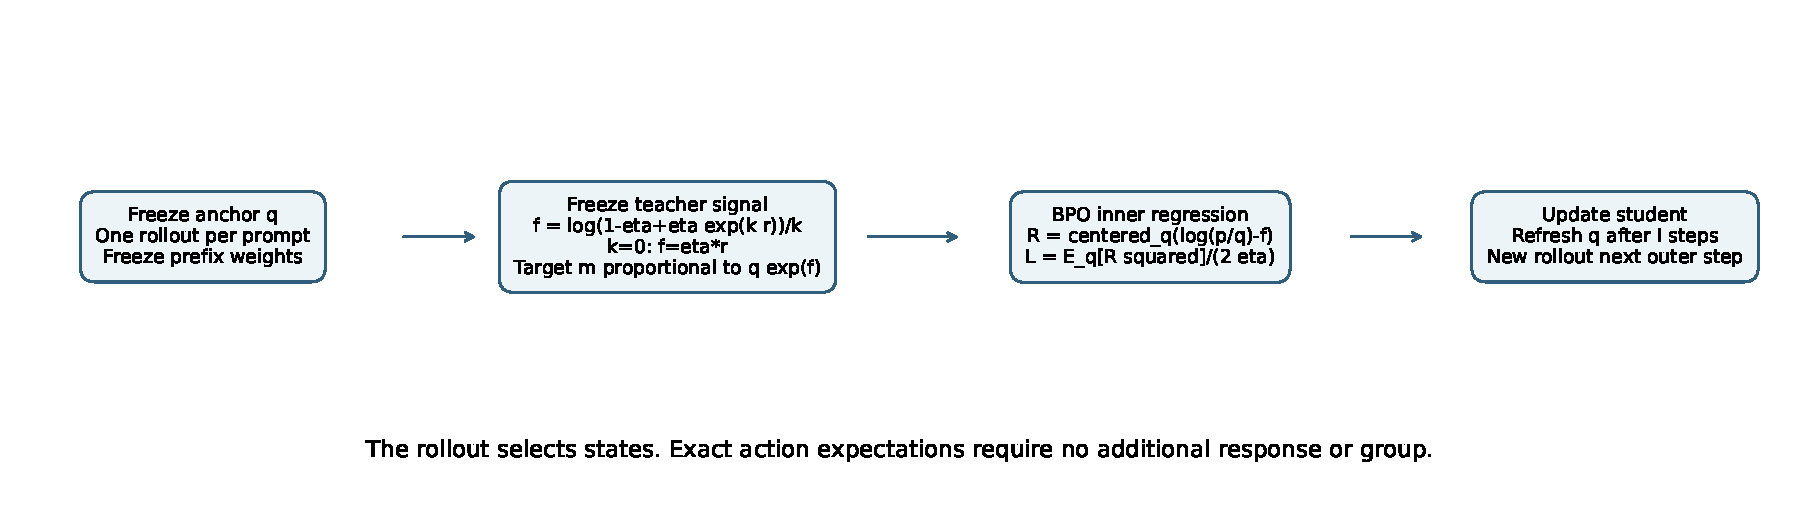
\includegraphics[width=\textwidth]{../../results/power-bpo-algorithm/pipeline.pdf}
 \caption{一条 response 选择前缀，幂均值形状决定冻结监督，BPO 以冻结 $q$ 的条件方差拟合。完整词表求和不需要增加 response 数量。}
\end{figure}
\begin{figure}[htbp]
 \centering
 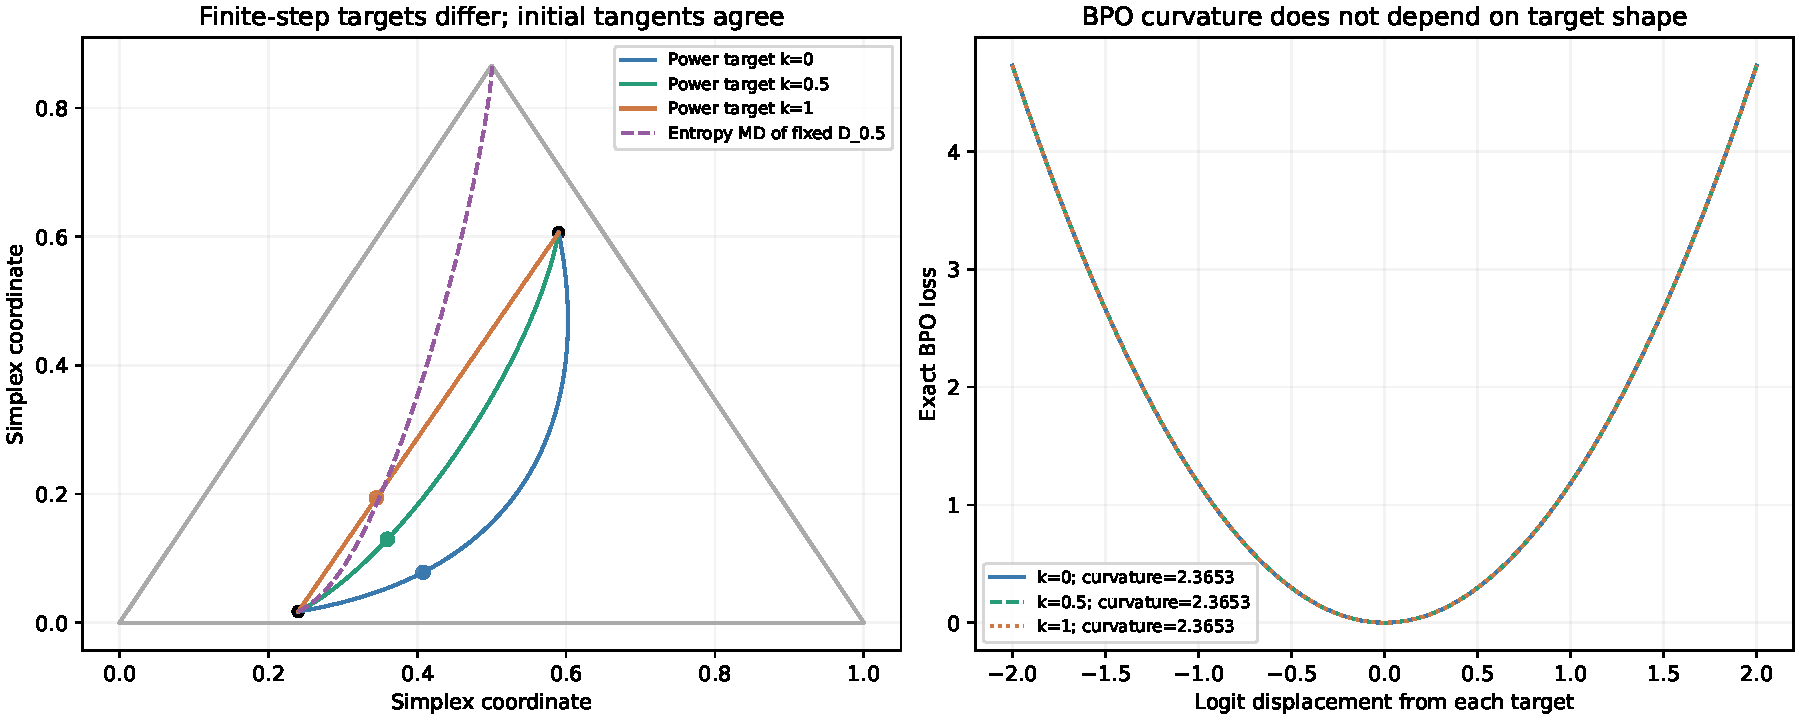
\includegraphics[width=\textwidth]{../../results/power-bpo-algorithm/geometry-and-curvature.pdf}
 \caption{左：幂均值有限步路径与固定 $D_{1/2}$ 的 entropy MD 路径只有起始切向量一致。右：不同 target 只平移固定 $q,\eta$ 的 BPO 二次损失，曲率不随 $\kappa$ 改变。}
\end{figure}

% END SOURCE: sections/proximal_bpo_algorithm.tex


\section{教师监督的方差与误差控制}
\label{sec:proximal-teacher-center}

% BEGIN SOURCE: book/sections/proximal_moment_bounds.tex
\subsection{固定插值强度的统一二阶矩界}

本节先给所有 $0<\kappa\le1$、$0<\eta<1$ 都适用的上界，再分析小 $\eta$ 时的锐阶数。记未归一化信号为 $f_{\kappa,\eta}(r)=\kappa^{-1}\log(1-\eta+\eta e^{\kappa r})$，BPO 教师监督为 $A=f/\eta$。关于 $f$ 的二阶矩不能省去这一次 $1/\eta^2$ 缩放后直接称为 BPO 梯度方差。

\begin{theorem}[幂均值信号的统一二阶矩界]
\label{thm:proximal-power-variance}
有限词表上 $q_a,T_a>0$，$0<\kappa\le1$、$0<\eta<1$。令
\begin{equation}
 C_\star=\sup_{u>0}\frac{\log^2(1+u)}u<\infty,\qquad
 B_{\kappa,\eta}=\frac{\log^2(1-\eta)+C_\star\eta}{\kappa^2}.
\end{equation}
则 $\E_qf^2\le B_{\kappa,\eta}$、$\E_qA^2\le B_{\kappa,\eta}/\eta^2$。若 $\|\psi(a)\|\le S$，有
\begin{equation}
 \Var_q[\psi C_qA]\le S^2\Var_qA
 \le S^2B_{\kappa,\eta}/\eta^2.
\end{equation}
该界不依赖词表维数。对 $\kappa=0$，一般不存在有限分布无关上界。
\end{theorem}

\begin{proof}
记 $\rho=T/q$。在 $\rho<1$ 上，$\log(1-\eta)/\kappa\le f<0$，负区域二阶矩不超过 $\log^2(1-\eta)/\kappa^2$。在 $\rho\ge1$ 上，
\begin{equation}
 0\le f\le\kappa^{-1}\log(1+\eta\rho^\kappa),\qquad
 f^2\le C_\star\eta\rho^\kappa/\kappa^2.
\end{equation}
由 $x^\kappa$ 的凹性与 $\E_q\rho=1$，有 $\E_q\rho^\kappa\le1$。合并两个区域得到 $\E_qf^2$ 上界；$A=f/\eta$ 给出监督的上界。常数有限，因为 $\log^2(1+u)/u$ 在零处和无穷处都趋零，在中间连续。梯度协方差 trace 不超过其二阶矩，而 $\E_q\|\psi C_qA\|^2\le S^2\Var_qA$。几何端点的发散由第~\ref{sec:power-setup}~节的二元反例给出。
\end{proof}

% END SOURCE: sections/proximal_moment_bounds.tex


% BEGIN SOURCE: book/sections/proximal_barycenter_moments.tex
\subsection{小插值强度的最坏二阶矩存在形状阈值}

固定 $\kappa>0$ 时，上一小节的统一 $O(\eta)$ 界还可以加强。这里考察完整支持概率分布上的最坏即时信号二阶矩
\begin{equation}
 \mathcal B_\kappa(\eta)
 =\sup_{q,T}\E_q\left[
 \left(\frac1\kappa\log(1-\eta+\eta(T/q)^\kappa)\right)^2
 \right].
\end{equation}
上界对任何有限维数成立；下界的二元见证已足够。它是未标准化的冻结信号，不含 student 残差。

\begin{theorem}[最坏二阶矩的精确小强度阶数]
\label{thm:proximal-moment-threshold}
对任意固定 $0<\kappa\le1$，当 $\eta\to0$ 时
\begin{equation}
 \mathcal B_\kappa(\eta)=\Theta_\kappa\left(\eta^{\min\{2,1/\kappa\}}\right).
 \label{eq:proximal-sharp-moment-order}
\end{equation}
$\Theta_\kappa$ 中的常数可依赖 $\kappa$，不依赖词表维数。几何端点则满足 $\mathcal B_0(\eta)=\infty$，对任意 $\eta>0$ 成立。
\end{theorem}

\begin{proof}
记 $\rho=T/q$。负区域 $\rho<1$ 的二阶矩不超过 $\log^2(1-\eta)/\kappa^2=O_\kappa(\eta^2)$。在正区域，$0\le f\le\log(1+\eta\rho^\kappa)/\kappa$。

若 $0<\kappa\le1/2$，用 $\log(1+x)\le x$ 与 $\E_q\rho^{2\kappa}\le1$ 得到
\begin{equation}
 \E_q[f^2\mathbf1\{\rho\ge1\}]
 \le\frac{\eta^2}{\kappa^2}\E_q\rho^{2\kappa}
 \le\frac{\eta^2}{\kappa^2}.
\end{equation}
所以 $\mathcal B_\kappa(\eta)\le[\log^2(1-\eta)+\eta^2]/\kappa^2=O_\kappa(\eta^2)$。取任一固定完整支持且 $q\ne T$ 的二元分布，逐项 Taylor 展开给出 $f/\eta\to(\rho^\kappa-1)/\kappa$。有限项求和后 $\E_qf^2/\eta^2\to\E_q(\rho^\kappa-1)^2/\kappa^2>0$，得到匹配的下界。

若 $1/2<\kappa\le1$，令 $s=1/\kappa\in[1,2)$。常数 $C_s=\sup_{x>0}\log^2(1+x)/x^s$ 有限，因为比值在零点按 $x^{2-s}$ 趋零，在无穷处也趋零。于是
\begin{equation}
 \E_q[f^2\mathbf1\{\rho\ge1\}]
 \le\frac{C_s\eta^s}{\kappa^2}\E_q\rho^{\kappa s}
 =\frac{C_s\eta^{1/\kappa}}{\kappa^2}.
\end{equation}
负区域的 $O(\eta^2)$ 比这个阶数更小。为证明下界，取 $T=(1/2,1/2)$、$q_1=\tfrac12\eta^{1/\kappa}$、$q_2=1-q_1$。第一项满足 $\rho_1=\eta^{-1/\kappa}$、$f_1=\log(2-\eta)/\kappa$，所以
\begin{equation}
 \E_qf^2\ge q_1f_1^2
 =\frac{\eta^{1/\kappa}}{2\kappa^2}\log^2(2-\eta)
 =\Omega_\kappa(\eta^{1/\kappa}).
\end{equation}
上下界匹配。$\kappa=1/2$ 已由第一种情况覆盖，也可取 $s=2$、$C_2=1$。$\kappa=0$ 时 $f=\eta\log(T/q)$，固定有正质量的 $q$ 并令对应 teacher 概率趋零，二阶矩无界。\hfill$\square$
\end{proof}

这个阶数区分了“固定分布的小步展开”与“对所有分布统一的小步上界”。固定 $q,T$ 时，对每个 $\kappa$ 都有 $\E_qf^2=O(\eta^2)$；最坏情形允许 $q,T$ 随 $\eta$ 改变，$\kappa>1/2$ 的稀有正尾部因此留下更慢的 $\eta^{1/\kappa}$ 阶数。算术端点为 $\Theta(\eta)$，平方根点为 $\Theta(\eta^2)$，二者的差异来自采样二阶矩，不是两种学习率单位。

若 score 范数不超过 $S$，定理给即时 score 估计与精确条件中心化估计相同阶数的方差上界，因为 $\Var(\psi f)\le S^2\E_qf^2$、$\Var(\psi C_qf)\le S^2\E_qf^2$。BPO 使用 $A=f/\eta$，对应界还需除以 $\eta^2$。它没有证明所有参数化模型都达到这个最坏阶数，也没有覆盖随机标准差归一化后的信号。

\begin{theorem}[监督高阶矩的形状阈值]
\label{thm:power-general-moment-threshold}
固定实数 $p\ge1$、$0<\kappa\le1$，令 $\eta\to0$。对全部有限词表、正支持分布取上确界，有
\begin{align}
 \sup_{q,T}\E_q|A_{\kappa,\eta}|^p
 &=\Theta_{\kappa,p}\!\left(\eta^{\min\{p,1/\kappa\}-p}\right),\\
 \sup_{q,T}\E_q|C_qA_{\kappa,\eta}|^p
 &=\Theta_{\kappa,p}\!\left(\eta^{\min\{p,1/\kappa\}-p}\right).
\end{align}
小步极限具有统一 $p$ 阶矩界的区间为 $0<\kappa\le1/p$。几何端点对任何正 $\eta$ 都无有限统一矩界。
\end{theorem}

\begin{proof}
先估计 $f=\eta A$。负区域的 $p$ 阶矩不超过 $|\log(1-\eta)/\kappa|^p=O_{\kappa,p}(\eta^p)$。若 $p\kappa\le1$，正区域用 $\log(1+x)\le x$ 及 $\E_q\rho^{p\kappa}\le1$，得到 $\E_q|f|^p=O_{\kappa,p}(\eta^p)$。若 $p\kappa>1$，令 $s=1/\kappa<p$，则 $C_{p,s}=\sup_{x>0}\log^p(1+x)/x^s<\infty$，因为该比值在零处按 $x^{p-s}$ 趋零，在无穷处也趋零。于是正区域的矩不超过 $C_{p,s}\eta^s\E_q\rho^{\kappa s}/\kappa^p=O_{\kappa,p}(\eta^{1/\kappa})$。除以 $\eta^p$ 得第一式上界。

当 $p\kappa\le1$，任一固定非同分布的二元 $q,T$ 使 $A$ 及 $C_qA$ 的小步极限具有严格正的 $p$ 阶矩，得到常数级下界。当 $p\kappa>1$，取 $q_1=\eta^{1/\kappa}/2$、$T_1=1/2$。稀有项 $A_1=\log(2-\eta)/(\kappa\eta)$，常见项 $A_2=O(1)$，所以 $q_1|A_1|^p=\Omega_{\kappa,p}(\eta^{1/\kappa-p})$。二元中心化后稀有项为 $(1-q_1)(A_1-A_2)$，仍有相同阶数。最后，对任意输入，Jensen 与 $|x-y|^p\le2^{p-1}(|x|^p+|y|^p)$ 给出 $\E|C_qA|^p\le2^p\E|A|^p$，从而第二式上界成立。几何端点用固定正质量的 $q$ 和趋零的教师概率得到发散。
\end{proof}

平方根点控制统一二阶矩；若要求小步极限中的统一四阶矩，则需要 $\kappa\le1/4$。这提供另一种明确的形状选择标准，并不表示 $\kappa=1/4$ 对每个输入的方差更小。

\begin{figure}[htbp]
 \centering
 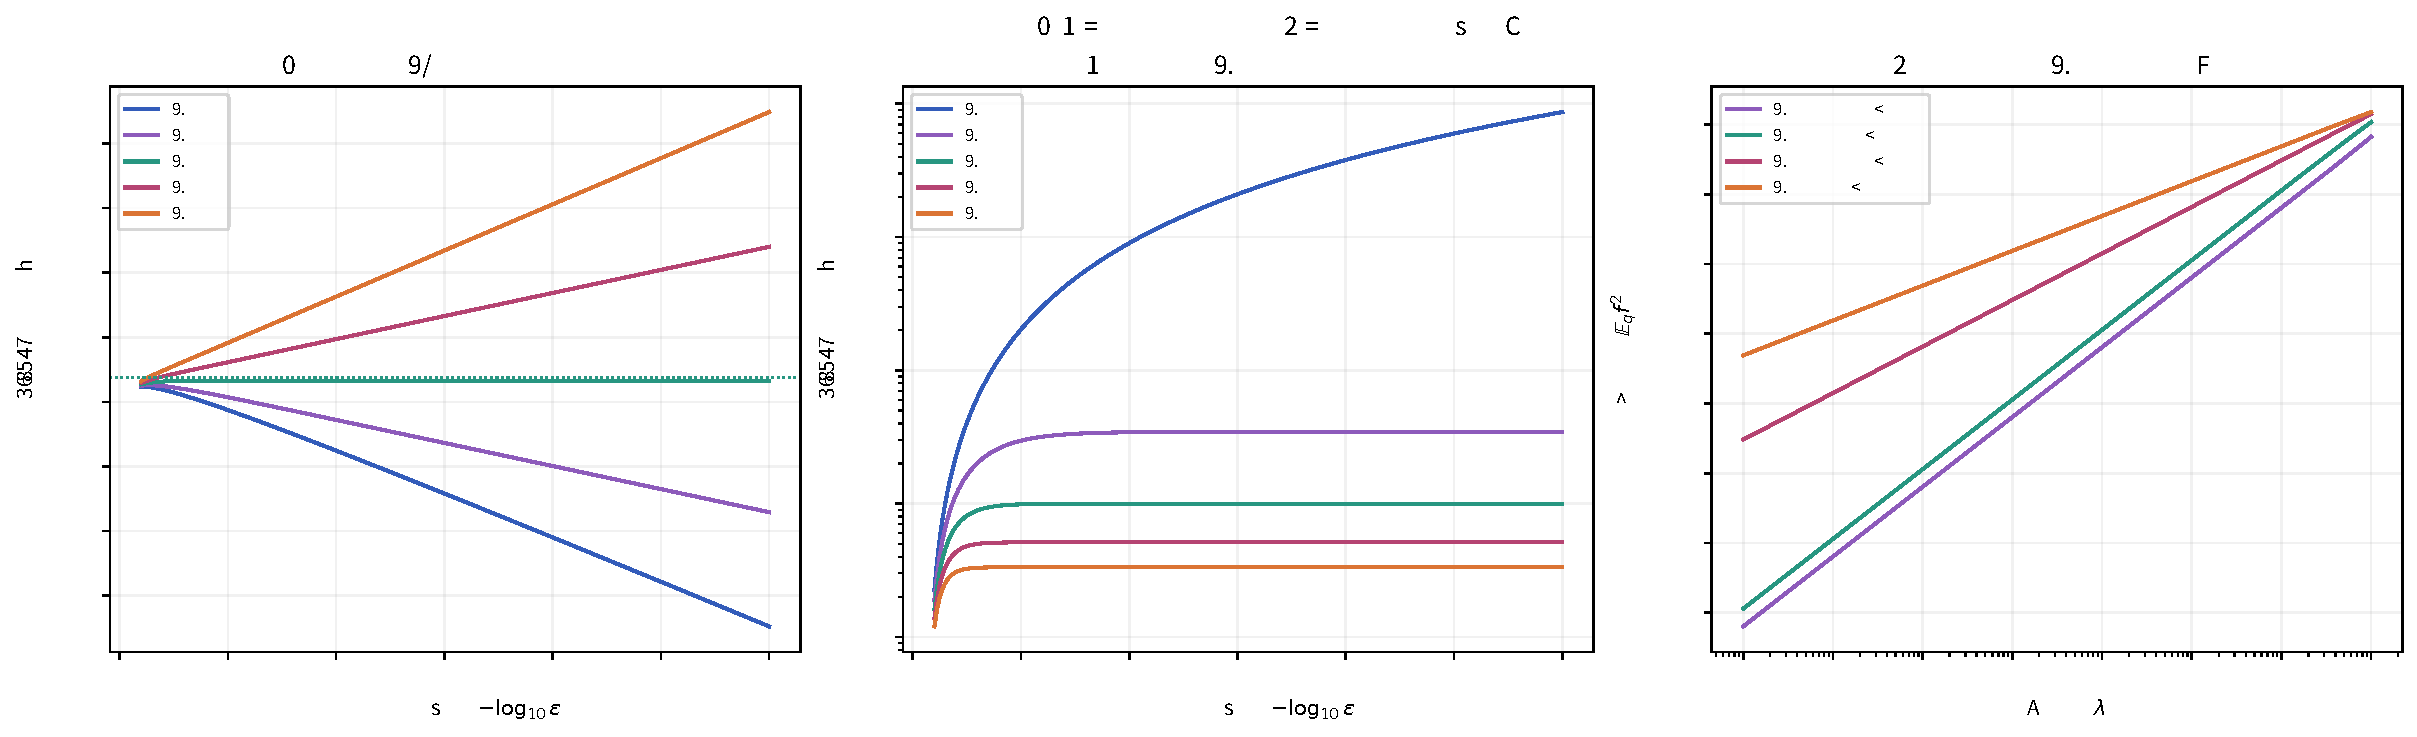
\includegraphics[width=\textwidth]{../../results/proximal-family-geometry/threshold.pdf}
 \caption{形状阈值的解析见证。左图让学生概率趋零，$\kappa>1/2$ 的自然梯度 Fisher 速度发散；中图让 teacher 概率趋零，几何端点的速度发散；右图使用随 $\eta$ 改变的二元 anchor，信号二阶矩斜率分别趋于 $2,2,4/3,1$。右图不是对所有分布做数值最大化，其作用是验证证明中的下界见证。}
\end{figure}

% END SOURCE: sections/proximal_barycenter_moments.tex


% BEGIN SOURCE: book/sections/proximal_teacher_center.tex
本节使用式~\eqref{eq:center-explicit-definition} 的 $A,K,B$。固定前缀、严格正且归一化的 $q,T$，$\rho=T/q$、$0\le\kappa\le1$、$0<\eta<1$。中心 $K$ 已经含有 $1/\eta$；若缓存原始信号中心 $\widetilde K=-\E_qf$，则 $\widetilde K=\eta K$，BPO 系数不再重复缩放。教师信号与中心在 inner 冻结，学生反馈 $C_qU/\eta$ 随参数改变。

\subsection{完整展开、KL 端点与凸散度表示}

两个 KL 端点及插值强度的边界为
\begin{align}
 K_{0,\eta}&=\KL(q\Vert T),\\
 K_{1,\eta}&=\eta^{-1}\KL\big(q\Vert(1-\eta)q+\eta T\big),\\
 K_{\kappa,1}&=\KL(q\Vert T).
 \label{eq:divergence-map-center-endpoints}
\end{align}
一般形状则为
\begin{equation}
 \boxed{K_{\kappa,\eta}
 =-\frac1{\kappa\eta}\sum_aq_a
 \log\left(1-\eta+\eta(T_a/q_a)^\kappa\right).}
 \label{eq:center-expanded-k}
\end{equation}
一般 $\kappa$ 下，若 $m$ 是归一化幂均值 target、$Z=\sum_aq_ae^{f_a}$，则
\begin{equation}
 K_{\kappa,\eta}=\frac{\KL(q\Vert m)-\log Z}{\eta}.
\end{equation}
所以不能把它继续标为原 teacher KL。

中心 $K$ 也属于凸 $f$ 散度。对 $\kappa>0$ 定义
\begin{equation}
 \phi_{\kappa,\eta}(x)=x-1-
 \frac{\log(1-\eta+\eta x^\kappa)}{\kappa\eta},\qquad x>0.
 \label{eq:center-convex-generator}
\end{equation}
它满足 $\phi(1)=\phi'(1)=0$，且
\begin{equation}
 \phi''(x)=
 \frac{x^{\kappa-2}[(1-\kappa)(1-\eta)+\eta x^\kappa]}
 {(1-\eta+\eta x^\kappa)^2}>0.
\end{equation}
因此 $\phi(x)\ge0$，再由 $\E_q(\rho-1)=0$，得到
\begin{equation}
 K_{\kappa,\eta}=\E_q\phi_{\kappa,\eta}(T/q).
 \label{eq:divergence-map-center-family}
\end{equation}
这个式子的标准 $f$-divergence 参照测度是 $q$，第一分布是 $T$；其生成函数包含 $\kappa,\eta$。对 $\kappa=0$，直接使用 $\phi_0(x)=x-1-\log x$。它与普通 KL 或前文 $D_\kappa$ 的关系由上述端点和极限决定，不能因其非负就把名称混用。
\subsection{中心的有界性、单调性与小步极限}

\begin{theorem}[教师中心的分布无关界]
\label{thm:center-bounds-monotonicity}
令 $0<\kappa\le1$、$0<\eta<1$，则
\begin{equation}
 0\le K_{\kappa,\eta}
 \le\min\left\{\KL(q\Vert T),\;
 c_{\kappa,\eta}\right\},\qquad
 c_{\kappa,\eta}=-\frac{\log(1-\eta)}{\kappa\eta}.
 \label{eq:center-uniform-cap}
\end{equation}
$K=0$ 当且仅当 $q=T$。固定 $q,T$ 时，$K$ 随 $\kappa$ 非增加、随 $\eta$ 非减少。对任意至少二元的词表，上界 $c_{\kappa,\eta}$ 是对完整支持分布取上确界的锐值。
\end{theorem}

\begin{proof}
凸生成函数给出非负性和零点唯一性。逐 action 有 $A\ge\log(1-\eta)/(\kappa\eta)=-c$，取负均值得到 $K\le c$。加权 AM--GM 不等式给出 $1-\eta+\eta\rho^\kappa\ge\rho^{\kappa\eta}$，故 $A\ge\log\rho$，得到 $K\le\KL(q\Vert T)$。

固定 $r=\log\rho$，令 $H(k)=\log(1-\eta+\eta e^{kr})$。$H(0)=0$ 且
\begin{equation}
 H''(k)=\frac{\eta(1-\eta)r^2e^{kr}}{(1-\eta+\eta e^{kr})^2}\ge0.
\end{equation}
凸函数从零点出发的割线斜率 $H(k)/k$ 非减少，因此 $A=H(k)/(k\eta)$ 随 $k$ 非减少，$K$ 非增加。

固定 $k>0$，记 $x=\rho^k-1>-1$、$y=1+\eta x>0$，则
\begin{equation}
 \partial_\eta A=\frac{1-y^{-1}-\log y}{k\eta^2}\le0,
\end{equation}
因为 $\log y-1+y^{-1}\ge0$。取负期望得到 $K$ 随 $\eta$ 非减少。

为证明锐性，取 $q=(\epsilon,1-\epsilon)$、$T=(1-\epsilon^2,\epsilon^2)$，$\epsilon\to0$。常见 action 的比率趋零，$-A\to c$；稀有 action 对 $K$ 的贡献为 $O(\epsilon\log\epsilon)$，趋零。因此 $K\to c$。所有有限 $\epsilon>0$ 都保持完整支持。\hfill$\square$
\end{proof}

该上界控制的是新的鲁棒散度，不是原 teacher KL 的上界；$K$ 有界并不意味着 $\KL(q\Vert T)$ 有界。作为固定参数的凸散度，$K$ 可以继承第~\ref{thm:power-bpo-inner-all-f}~定理的理想 teacher 保持路径单调性，但训练中缓存的 $K(q_n,T)$ 在整个 inner 窗口本来就是常数，不能把它当成不断变化的拟合误差。

当 $\eta=1$ 时全部形状恢复 $A=\log\rho$、$K=\KL(q\Vert T)$，不再具有上面的有限分布无关上界。当 $\kappa\to0$ 时上界也发散；原 KL 没有自动获得有界性。

对固定完整支持 $q,T$，Taylor 展开给出
\begin{align}
 A_{\kappa,\eta}&\longrightarrow\frac{\rho^\kappa-1}{\kappa},\label{eq:divergence-map-center-limit}\\
 K_{\kappa,\eta}&\longrightarrow
 \frac{1-a_\kappa}{\kappa},\qquad
 a_\kappa=\sum_aq_a^{1-\kappa}T_a^\kappa.
 \label{eq:center-small-step-limit}
\end{align}
$0<\kappa<1$ 时此极限是 $(1-\kappa)D_\kappa(T\Vert q)$；$\kappa=1$ 的极限为零。由 $\log(1+\eta x)\le\eta x$，这个极限同时给出有限 $\eta$ 的下界 $K\ge(1-a_\kappa)/\kappa$。

平方根点尤其简单：
\begin{equation}
 \lim_{\eta\to0}K_{1/2,\eta}
 =2\left(1-\sum_a\sqrt{q_aT_a}\right)
 =\sum_a(\sqrt{q_a}-\sqrt{T_a})^2=:H^2(q,T)\le2.
\end{equation}
这里明确采用不带 $1/2$ 因子的平方 Hellinger 距离。

当 $\rho=1+\delta$ 且全部比率一致接近一时，生成函数在一附近展开为
\begin{equation}
 K_{\kappa,\eta}
 =\frac{1-\kappa(1-\eta)}2\chi^2(T\Vert q)
  +O(\E_q|\delta|^3).
\end{equation}
这描述局部教师差异；对任意极端概率比不能使用这个 Taylor 余项作统一保证。
\subsection{Advantage 的单侧界与误差相关方差界}

精确中心化不改变标量方差：
\begin{equation}
 V_{\kappa,\eta}:=\Var_q(B)=\Var_q(A).
\end{equation}
因此 $K$ 使均值归零，但标量方差的改变来自 $A$ 的形状变换。 这里限定为固定 prefix。跨冻结状态测度 $d$ 的总方差满足
\begin{align}
 \Var_{d,q}(A)&=\E_dV_s+\Var_d(K_s),\\
 \Var_{d,q}(B)&=\E_dV_s.
\end{align}
因此按 prefix 精确中心化会移除不同 prefix 的监督均值差异，$\kappa=0$ 也有这项标量收益；它不等于降低条件 action 方差，也不自动降低带 score 权重的参数梯度方差。

由前面的逐 action 下界，
\begin{equation}
 B(a)\ge K_{\kappa,\eta}-c_{\kappa,\eta}\ge-c_{\kappa,\eta}.
\end{equation}
没有不依赖 $q,T$ 的逐 action 正上界：当 $q_a\to0$ 而 $T_a$ 保持正质量，$A_a$ 按 $\log(T_a/q_a)/\eta$ 增长。单侧有界、方差有界与双侧有界是不同结论。

对任何固定 $\kappa>0,\eta<1$，仍然存在统一的有限方差界。在 $A>0$ 区域，$A\le\log\rho/\eta$；Markov 不等式与 $\E_q\rho=1$ 给出 $\Pr(A>x)\le e^{-\eta x}$、$x\ge0$。因此
\begin{equation}
 V\le\E_qA^2\le c_{\kappa,\eta}^2+2/\eta^2.
\end{equation}
下面的平方根阈值涉及 $\eta\to0$ 时能否保持常数级统一界，不表示较大 $\kappa$ 在固定正 $\eta$ 下完全没有方差界。

\begin{theorem}[中心化教师 advantage 的方差控制]
\label{thm:center-advantage-variance}
若 $0<\kappa\le1/2$、$0<\eta<1$，则
\begin{align}
 V_{\kappa,\eta}
 &\le\frac{1-a_\kappa^2}{\kappa^2(1-\eta)^2}
 \le\frac1{\kappa^2(1-\eta)^2},\\
 V_{\kappa,\eta}
 &\le\frac{D_\kappa(T\Vert q)}{\kappa(1-\eta)^2}
 \le\frac{K_{\kappa,\eta}}{\kappa(1-\kappa)(1-\eta)^2}.
 \label{eq:center-error-scaled-variance}
\end{align}
这两个界均不依赖词表维数或概率的统一正下界。
\end{theorem}

\begin{proof}
令 $X=\rho^\kappa$、$h(X)=\log(1-\eta+\eta X)/(\kappa\eta)$。对 $X\ge0$，$|h'|\le1/[\kappa(1-\eta)]$。若 $X'$ 是独立同分布副本，方差的成对表示给出
\begin{equation}
 \Var h(X)=\frac12\E(h(X)-h(X'))^2
 \le\frac{\Var X}{\kappa^2(1-\eta)^2}.
\end{equation}
由于 $2\kappa\le1$，Jensen 不等式给出 $\E_q\rho^{2\kappa}\le1$，因此 $\Var X\le1-a_\kappa^2$，得到第一条界。为收紧误差相关常数，令 $a(u)=\E_q\rho^u$。对 $u$ 求二阶导数，$a''(u)=\E_q[\rho^u\log^2\rho]\ge0$；由 $2\kappa\in[\kappa,1]$、$a(1)=1$，凸性给出
\begin{align}
 a(2\kappa)&\le\frac{1-2\kappa}{1-\kappa}a(\kappa)+\frac{\kappa}{1-\kappa},\\
 \Var X&\le\frac{[1-a(\kappa)][\kappa+(1-\kappa)a(\kappa)]}{1-\kappa}
 \le\frac{1-a(\kappa)}{1-\kappa}.
\end{align}
因此 $\Var X/\kappa^2\le D_\kappa(T\Vert q)/\kappa$。再由 $K\ge[1-a(\kappa)]/\kappa=(1-\kappa)D_\kappa(T\Vert q)$，得到误差相关两条界。旧的简便界 $2K/[\kappa(1-\eta)^2]$ 仍成立，但在 $\kappa<1/2$ 时比新界更松。
\hfill$\square$
\end{proof}

在 inner 起点，若 score 范数不超过 $S$，teacher score 抽样满足 $\Var(g)\le S^2V\le S^2K/[\kappa(1-\kappa)(1-\eta)^2]$。这是带 score 条件的误差相关噪声界，不是全模型无条件性质。

平方根点有 $V\le4K/(1-\eta)^2$，并在小步极限得到精确关系
\begin{equation}
 \lim_{\eta\to0}V_{1/2,\eta}
 =4(1-a_{1/2}^2)=H^2(4-H^2)\le4.
\end{equation}
因此该极限的教师中心与 advantage 方差同时有界，且教师差异趋零时方差也趋零。

前面的原始信号锐矩阶数还能加强为中心化后的结论：对固定 $0<\kappa\le1$，
\begin{equation}
 \sup_{q,T}V_{\kappa,\eta}
 =\Theta_\kappa\big(\eta^{\min\{2,1/\kappa\}-2}\big),\qquad\eta\to0.
\end{equation}
上界由 $\Var A\le\E A^2$ 和定理~\ref{thm:proximal-moment-threshold} 得到。$\kappa\le1/2$ 的下界取任一固定非同分布 $q,T$，小步极限的方差严格为正。$\kappa>1/2$ 时取 $q_1=\eta^{1/\kappa}/2$、$T_1=1/2$，则 $A_1=\log(2-\eta)/(\kappa\eta)$，而 $A_2$ 保持有限；二元方差 $q_1q_2(A_1-A_2)^2$ 给出匹配的下界。$\kappa=0$ 则对任意 $\eta$ 都无统一方差上界。这里允许最坏分布随 $\eta$ 改变，不能混同于固定分布上的连续极限。

更精确地，记第~\ref{sec:power-half-and-optimality}~节的锐 Fisher 速度常数为 $C_{\mathrm{vel}}(\kappa)=\sup_{q,T}\Var_q(\rho^\kappa)/\kappa^2$。上述 Lipschitz 证明给出 $V\le C_{\mathrm{vel}}/(1-\eta)^2$，而任意固定正支持分布的极限是 $\Var_q(\rho^\kappa)/\kappa^2$。先选择逼近上确界的固定分布、再令 $\eta\to0$，上下界夹逼得到
\begin{equation}
 \lim_{\eta\to0}\sup_{q,T}V_{\kappa,\eta}
 =C_{\mathrm{vel}}(\kappa),\qquad0<\kappa\le1/2.
\end{equation}
因此 $\kappa_\star=0.4419283735$ 也最小化最坏的小步标量 advantage 方差，其锐值为 $3.5272748442$；平方根点的值为 4。这个准则不是全参数梯度信噪比，也不是数学任务正确率。 几何端点甚至不能仅从 KL 小推出低方差：取 $q=(\epsilon,1-\epsilon)$、$T=(e^{-\epsilon^{-3/4}},1-e^{-\epsilon^{-3/4}})$，则 $K_{0,\eta}\sim\epsilon^{1/4}\to0$，但 $\Var_qB_{0,\eta}\sim\epsilon^{-1/2}\to\infty$。固定正形状和固定 $\eta<1$ 的负尾部饱和会在同一族上使方差降至 $O(\epsilon)$。


\begin{figure}[htbp]
 \centering
 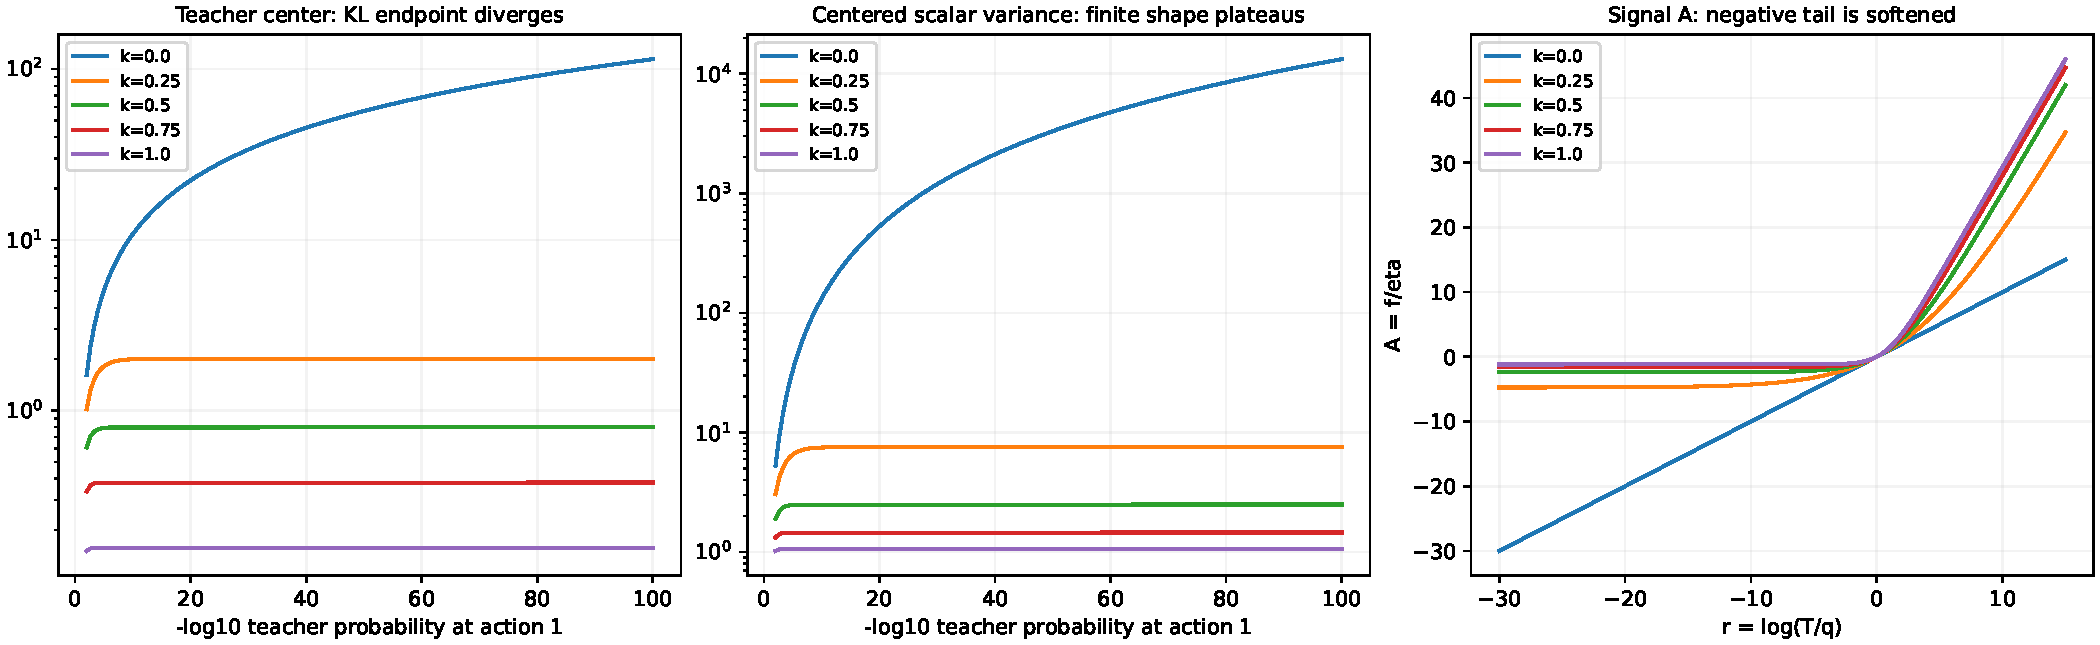
\includegraphics[width=\textwidth]{../../results/power-center-advantage/negative-tail-center-variance.pdf}
 \caption{固定 $q=(1/2,1/2)$、$\eta=0.3$，teacher 一个概率趋零时，几何中心及 advantage 方差发散，正形状出现平台。右图显示规范化信号 $A$ 的负尾部变化。曲线由完整二元分布精确求和生成。}
\end{figure}
\begin{figure}[htbp]
 \centering
 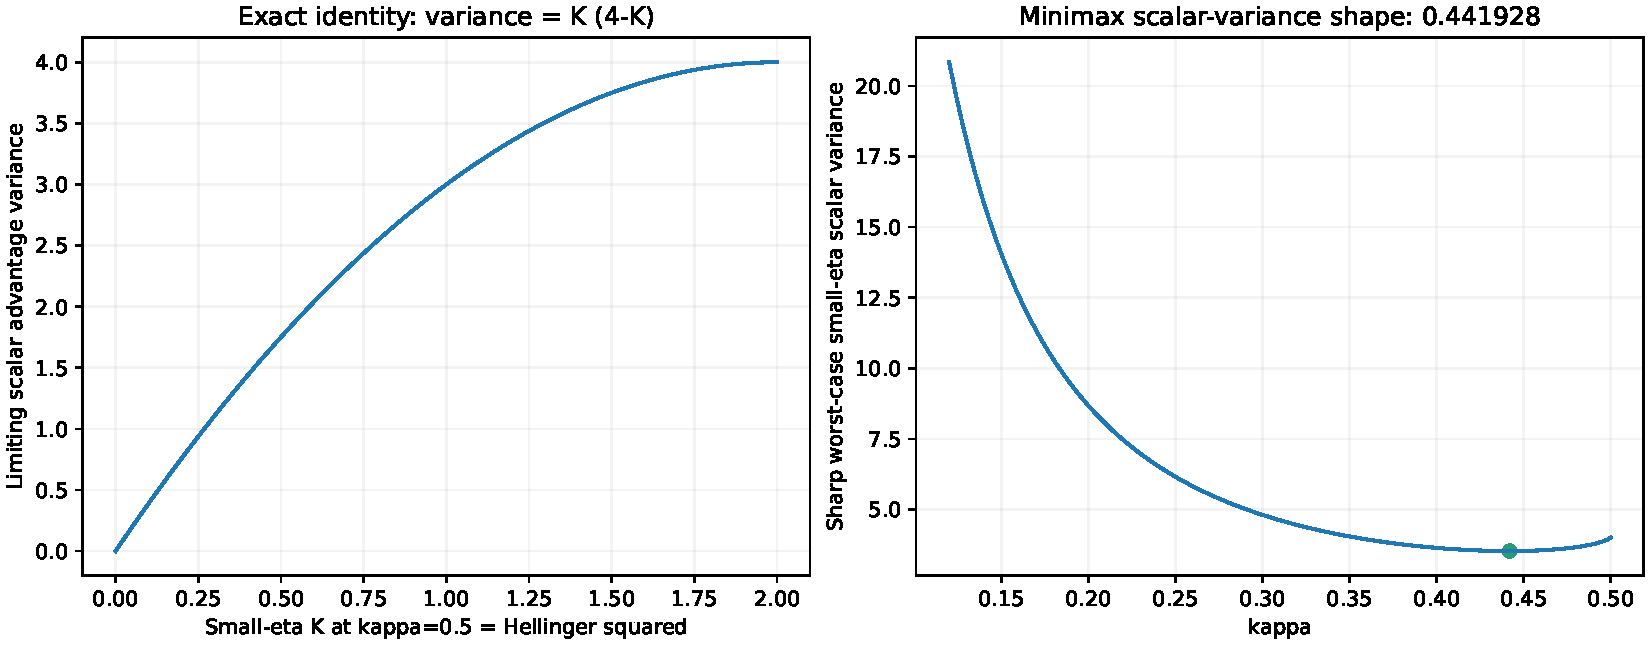
\includegraphics[width=\textwidth]{../../results/power-center-advantage/sharp-small-step-center-variance.pdf}
 \caption{左：平方根的小步极限满足 $V=K(4-K)$。右：最坏标量 advantage 方差的锐小步常数与前文自然速度常数一致，最优形状约为 $0.441928$。}
\end{figure}

% END SOURCE: sections/proximal_teacher_center.tex


% BEGIN SOURCE: book/sections/proximal_md_noise.tex
\subsection{中心作为 MD 目标的散度代理}

\begin{theorem}[教师中心与精确 MD 目标的比较]
\label{thm:power-md-center-comparison}
对 $0\le\kappa\le1$、$0<\eta<1$，有逐点生成函数界和散度界
\begin{align}
 (1-\kappa)\omega_{\kappa,\eta}(x)
 &\le\phi_{\kappa,\eta}(x)\le\omega_{\kappa,\eta}(x),\\
 (1-\kappa)\mathcal J_{\kappa,\eta}(q;T)
 &\le K_{\kappa,\eta}(q,T)\le\mathcal J_{\kappa,\eta}(q;T).
 \label{eq:power-md-center-sandwich}
\end{align}
当 $\kappa<1$，$K$ 与 $\mathcal J$ 可互相控制；当 $\kappa=0$ 时相等。一般 $\kappa>0,\eta<1$ 下，$-A(T/p)$ 是 $\mathcal J$ 的梯度，却不是 $K(T,p)$ 的梯度。
\end{theorem}

\begin{proof}
记 $B=1-\eta+\eta x^\kappa$，两种生成函数的曲率比为
\begin{equation}
 \frac{\phi''(x)}{\omega''(x)}
 =1-\frac{\kappa(1-\eta)}B\in[1-\kappa,1].
\end{equation}
故 $\phi-(1-\kappa)\omega$ 与 $\omega-\phi$ 均为凸函数，在一处的函数值和导数为零，因而处处非负。对概率比求期望得到散度界。要计算中心作为当前分布函数的梯度，应用透视函数微分公式，得到
\begin{align}
 \frac\partial{\partial p_a}K_{\kappa,\eta}(p,T)
 &=\phi(x)-x\phi'(x)\\
 &=-A(x)+\frac{x^\kappa}{1-\eta+\eta x^\kappa}-1,
 \qquad x=T_a/p_a.
 \label{eq:power-md-center-gradient-difference}
\end{align}
额外项在 $\kappa>0,\eta<1$ 时通常随 action 改变，不能作为单纯形上的常数乘子消去。$\kappa=0$ 或 $\eta=1$ 时该项为零。
\end{proof}

这个比较给出一个可用的误差解释：若固定 $\kappa<1$ 且精确中心 $K\le\epsilon$，则 $\mathcal J\le\epsilon/(1-\kappa)$。它控制新的教师目标，不控制任意大的原 teacher reverse KL；当 $\kappa$ 接近一时该代理界退化。

两个目标的局部尺度也不同。记 $\delta=T/q-1$ 且全部比率一致趋一，则
\begin{align}
 \mathcal J_{\kappa,\eta}(q;T)
 &=\tfrac12\E_q\delta^2+O(\E_q|\delta|^3),\\
 K_{\kappa,\eta}(q,T)
 &=\tfrac12[1-\kappa(1-\eta)]\E_q\delta^2+O(\E_q|\delta|^3).
\end{align}
依据是 $\omega''(1)=1$ 与 $\phi''(1)=1-\kappa(1-\eta)$，一次项均因规范化消失。$D_\kappa$ 与 $\mathcal J_{\kappa,\eta}$ 的二阶局部 Fisher 尺度相同，$K$ 额外带有形状相关系数；三个数值不能直接作为同一训练误差混合比较。

\begin{figure}[H]
 \centering
 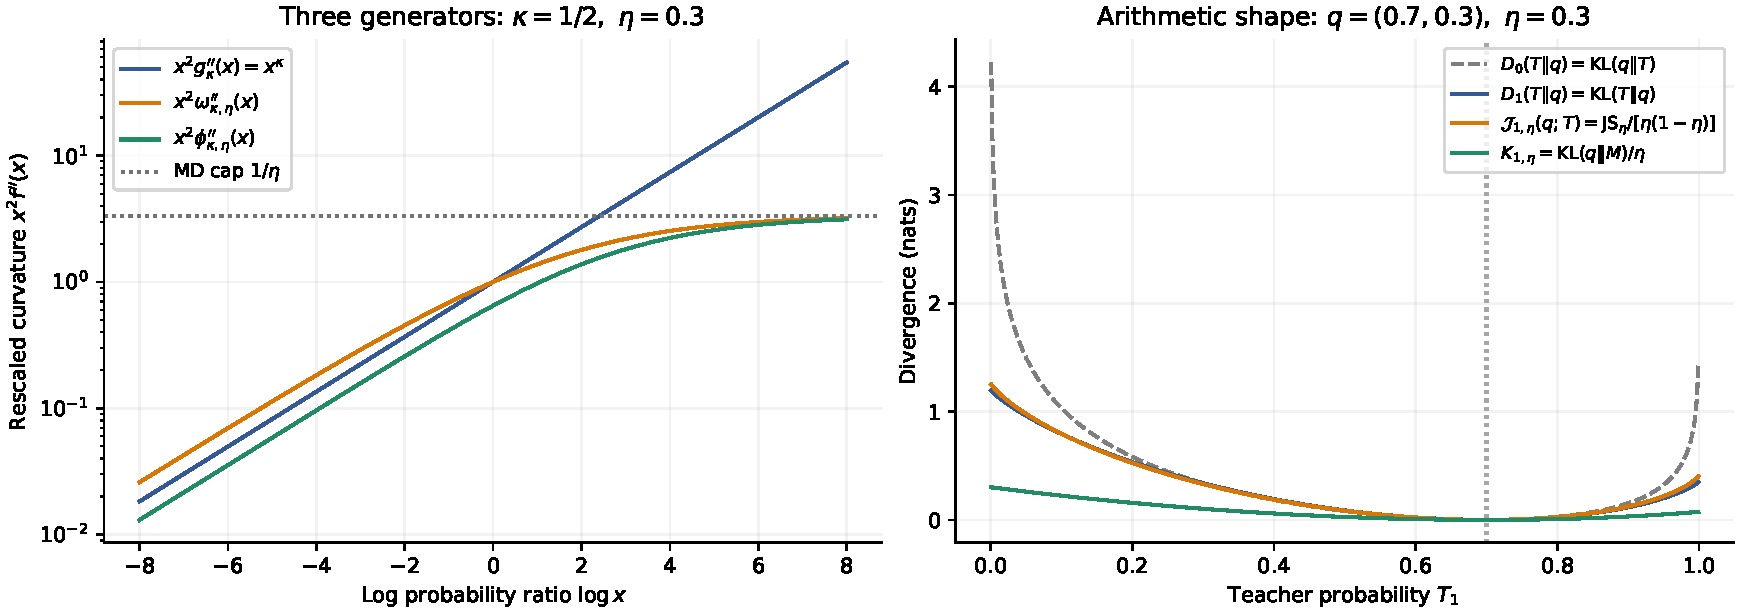
\includegraphics[width=\textwidth]{../../results/power-divergence-relations/families-and-curvature.pdf}
 \caption{三种散度的解析函数比较。左图在 $\kappa=1/2,\eta=0.3$ 时比较乘以 $x^2$ 的生成函数曲率；MD 曲率被 $1/\eta$ 统一控制，中心曲率更小。右图固定 $q=(0.7,0.3)$、$\eta=0.3$，让教师 $T=(T_1,1-T_1)$ 变化；算术形状的重心散度、精确 MD 目标和教师中心分别是 forward KL、归一化 JS 和对混合分布的 reverse KL。所有曲线直接计算公式，不来自训练或模型实验。}
 \label{fig:power-divergence-curvature}
\end{figure}

图的生成入口为 \path{experiments/plotting/plot_power_divergence_relations.py}；参数与公式范围保存在 \path{results/power-divergence-relations/figure.json}。

\begin{corollary}[精确外层的教师监督噪声可求和]
\label{cor:power-md-summable-variance}
固定 $0<\kappa\le1/2$、$0<\eta<1$，采用每步精确幂均值目标的外层 $q_{n+1}=m_{\kappa,\eta}(q_n,T)$。令
\begin{equation}
 V_n=\Var_{q_n}\!\left[A_{\kappa,\eta}(T/q_n)+K_{\kappa,\eta}(q_n,T)\right],
 \qquad C_0=\KL(T\Vert q_0).
\end{equation}
则对 $N\ge1$，
\begin{align}
 V_N&\le\frac{C_0}{\kappa(1-\kappa)(1-\eta)^2\eta N},\\
 \sum_{n=1}^N V_n&\le\frac{C_0}{\kappa(1-\kappa)(1-\eta)^2\eta}.
 \label{eq:power-md-summable-variance}
\end{align}
若各 outer 起点的 score 统一满足 $\|\psi_n(a)\|\le S$，则中心化 teacher score 单样本梯度的协方差 trace 也分别不超过右侧乘以 $S^2$。
\end{corollary}

\begin{proof}
第~\ref{thm:center-advantage-variance}~定理给出 $V_n\le K_n/[\kappa(1-\kappa)(1-\eta)^2]$；第~\ref{thm:power-md-center-comparison}~定理给出 $K_n\le\mathcal J(q_n;T)$。将两者与最后迭代界相乘，得到第一式。三点进展的望远镜求和给出 $\eta\sum_{n=1}^N\mathcal J(q_n;T)\le C_0$，代入得到第二式。梯度方差不超过其二阶矩，且 $\E_{q_n}\|\psi_n B_n\|^2\le S^2V_n$，得到带 score 的结论。
\end{proof}

可求和性针对同一固定 prefix、精确刷新分布和未标准化的教师监督。它并不比较每个输入上不同 $\kappa$ 的实际方差，也不覆盖任意神经网络 inner 残差或不断改变的 prefix 访问测度。该推论把“鲁棒散度有界”“新目标的精确 MD 下降”和“误差相关方差界”连接为一条完整论证；无需先做大模型扫描来确定这些条件性质。

% END SOURCE: sections/proximal_md_noise.tex


\section{平方根形状与最优性的判据}
\label{sec:power-half-and-optimality}

% BEGIN SOURCE: book/sections/proximal_half_geometry.tex
\subsection{平方根形状的有界自然梯度与显式动力学}

由式~\eqref{eq:proximal-natural-velocity}，$\|v_\kappa\|_F^2=\Var_q(\rho^\kappa)/\kappa^2$。当 $0<\kappa\le1/2$，$2\kappa\le1$，Jensen 不等式给出 $\E_q\rho^{2\kappa}\le(\E_q\rho)^{2\kappa}=1$，于是
\begin{equation}
 \|v_\kappa\|_F^2\le\frac{1-a_\kappa^2}{\kappa^2}\le\frac1{\kappa^2}.
 \label{eq:proximal-natural-speed-bound}
\end{equation}
该界对任意完整支持的 $q,T$ 成立，不需要给 teacher 或 student 指定统一概率下界。对于 $\kappa>1/2$，取 $q=(\varepsilon,1-\varepsilon)$、$T=(c,1-c)$，$0<c<1$ 固定，则
\begin{equation}
 \Var_q(\rho^\kappa)
 =\varepsilon(1-\varepsilon)
 \left[(c/\varepsilon)^\kappa-((1-c)/(1-\varepsilon))^\kappa\right]^2
 \sim c^{2\kappa}\varepsilon^{1-2\kappa}\longrightarrow\infty.
\end{equation}
几何端点 $\kappa=0$ 也没有统一界：固定 $q=(1/4,3/4)$、令 $T=(\varepsilon,1-\varepsilon)$，$\Var_q\log(T/q)$ 随 $\varepsilon\to0$ 发散。故 $0<\kappa\le1/2$ 是这个自然梯度族具有统一 Fisher 速度界的区间。确定性的 Fisher 速度与随机参数梯度方差是不同对象，不能把这个结论直接写成完整训练梯度的方差定理。

在平方根点 $\kappa=1/2$，$a=\sum\sqrt{qT}$，并有 $\E_q\rho=1$，因此
\begin{equation}
 \|v_{1/2}\|_F^2=4(1-a^2)\le4,\qquad
 D_{1/2}(T\Vert q)=4(1-a).
\end{equation}
由 Lyapunov 等式，连续流满足
\begin{equation}
 \frac{da}{dt}=1-a^2,
 \qquad a(t)=\tanh(t+\operatorname{artanh}a(0)),\quad q\ne T.
 \label{eq:proximal-hellinger-flow}
\end{equation}
证明是 $dD_{1/2}/dt=-4\,da/dt=-4(1-a^2)$，然后积分 $da/(1-a^2)=dt$。$q=T$ 时 $a=1$ 且流恒定。进一步，$D'=-(1+a)D$，由于 $0<a\le1$，有
\begin{equation}
 D(0)e^{-2t}\le D(t)\le D(0)e^{-t}.
\end{equation}
若写 $a=\cos\vartheta$，则 $d\vartheta/dt=-\sin\vartheta$。平方根形状既有球面解释，也有显式 teacher 接近度和有界 Fisher 速度。这使它成为一个有数学依据的候选点，尚不能据此断言其训练性能优于其他形状。

\begin{figure}[htbp]
 \centering
 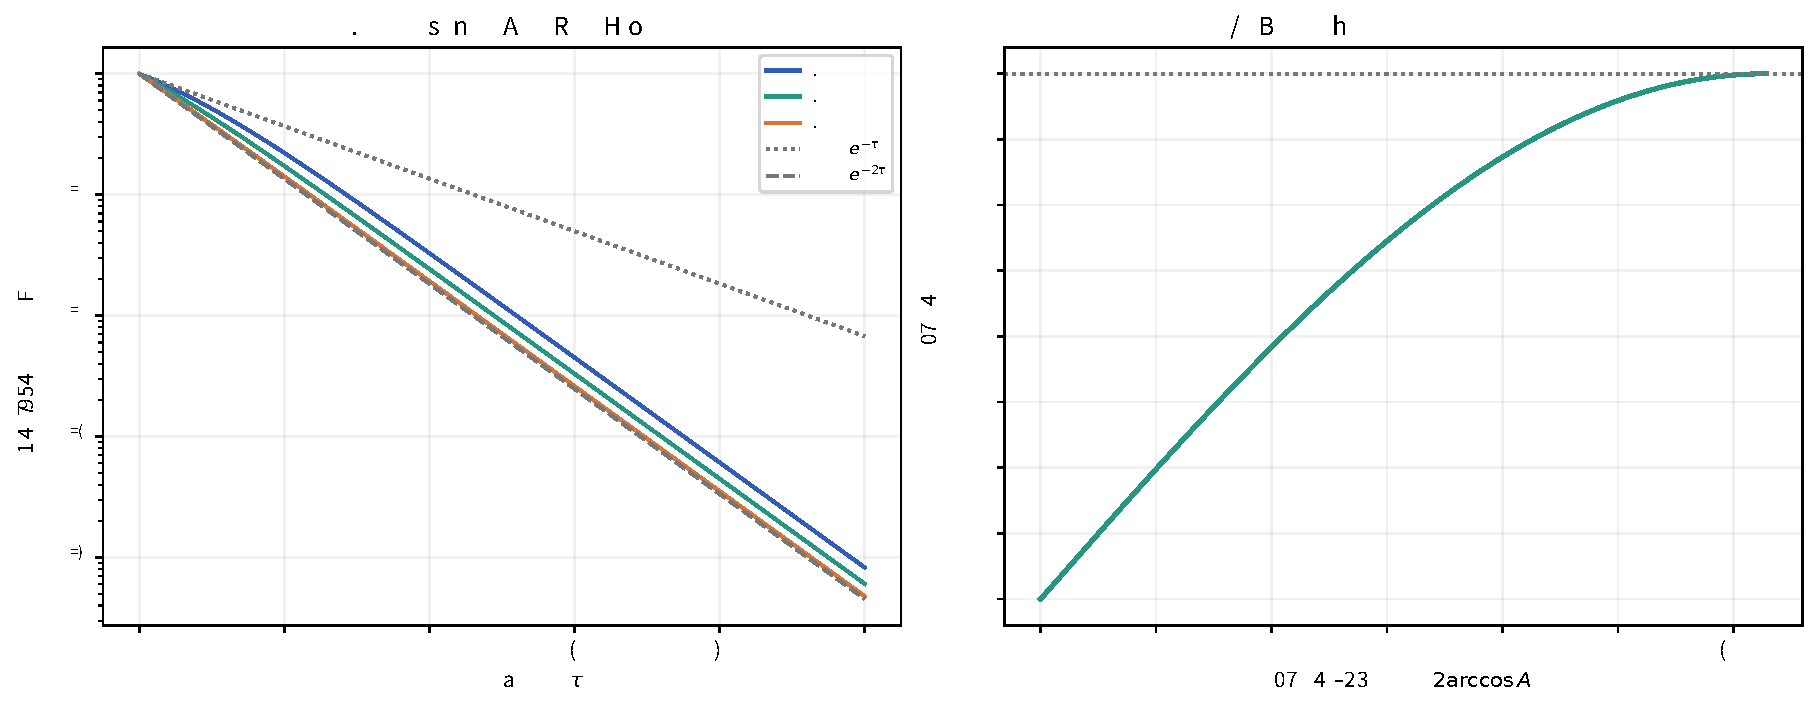
\includegraphics[width=\textwidth]{../../results/proximal-family-geometry/hellinger-flow.pdf}
 \caption{平方根形状的连续动力学。左图由 $a(t)=\tanh(t+\operatorname{artanh}a(0))$ 精确生成，归一化散度位于两个指数包络之间；右图将 Fisher 速度写成到 teacher 的 Fisher--Rao 距离函数，展示统一上界 2。}
\end{figure}

% END SOURCE: sections/proximal_half_geometry.tex


% BEGIN SOURCE: book/sections/proximal_shape_criteria.tex
\subsection{共同目标下的局部最优形状}

令 $r=\log(T/q)$，$w_\kappa=(\rho^\kappa-\E_q\rho^\kappa)/\kappa$，$w_0=C_qr$，于是 $v_\kappa=qw_\kappa$。对固定 Fisher 速度的单位方向 $u_\kappa=v_\kappa/\|v_\kappa\|_F$，reverse KL 的一阶下降量为
\begin{equation}
 -\nabla\KL(q\Vert T)^\top u_\kappa
 =\frac{\E_q[rw_\kappa]}{\sqrt{\E_qw_\kappa^2}}
 \le\sqrt{\Var_qr}.
\end{equation}
这是 Cauchy--Schwarz 不等式，几何形状 $\kappa=0$ 取得等号。对 forward KL，同样有
\begin{equation}
 -\nabla\KL(T\Vert q)^\top u_\kappa
 =\frac{\E_q[\rho w_\kappa]}{\sqrt{\E_qw_\kappa^2}}
 \le\sqrt{\Var_q\rho},
\end{equation}
算术形状 $\kappa=1$ 取得等号。更一般地，$\kappa$ 自己对应的散度具有自己的自然梯度最陡方向。这个局部确定性最优性与平方根形状的最坏矩性质是不同标准，不能由有界方差推出对任何共同评价目标的最优收敛速度。
\subsection{目标自然速度的锐上界与另一个极小极大形状}

对 $0<\kappa<1/2$，令 $X=\rho^\kappa$、$r=1/\kappa>2$，则 $\E_qX^r=1$。写成 $X^2=X^{(r-2)/(r-1)}(X^r)^{1/(r-1)}$，对两因子使用共轭指数 $(r-1)/(r-2)$ 与 $r-1$ 的 Hölder 不等式，得到
\begin{equation}
 \E_qX^2\le(\E_qX)^{(r-2)/(r-1)}
 =(\E_qX)^{(1-2\kappa)/(1-\kappa)}.
\end{equation}
令 $a=\E_qX\in[0,1]$，$\gamma=(1-2\kappa)/(1-\kappa)$。于是 $\Var_qX\le a^\gamma-a^2$。驻点满足 $a^{2-\gamma}=\gamma/2$，代回并记 $b=(1-2\kappa)/[2(1-\kappa)]$，得到锐上界
\begin{equation}
 \boxed{\sup_{q,T}\|v_\kappa\|_F^2
 =C_{\mathrm{vel}}(\kappa)
 =\frac{b^{1-2\kappa}(1-b)}{\kappa^2}}.
\end{equation}
锐性由 $q=(b,1-b)$、$T\to(1,0)$ 达到：$X$ 仅取 $b^{-\kappa}$ 与零，插值不等式和驻点条件同时成立。完整支持分布以极限逼近这个值。$\kappa=1/2$ 的上确界为 4；$\kappa=0$ 或 $\kappa>1/2$ 无有限上界。

在优化 $b$ 后使用包络导数，$d\log C_{\mathrm{vel}}/d\kappa=-2/\kappa-2\log b$。唯一最小点满足
\begin{equation}
 \log\frac{1-2\kappa_\star}{2(1-\kappa_\star)}=-\frac1{\kappa_\star}.
\end{equation}
左侧加 $1/\kappa$ 的导数为 $-1/[(1-2\kappa)(1-\kappa)]-1/\kappa^2<0$，在零点附近趋于正无穷，在 $1/2$ 附近趋于负无穷，故根唯一。根和常数由第一方参考函数 \texttt{minimax\_velocity\_shape}、\texttt{worst\_fisher\_speed\_squared} 计算并验证。

这个最优形状针对 target 的最坏 Fisher 速度上界及小步标量监督方差，与其他拟合散度的误差相关噪声常数最优 $\kappa_{\mathrm{fit}}=1/2$ 是不同标准。更小的最大速度不自动代表更快学习；部分 teacher 方向也可能变慢。平方根的闭式性质和这个极小极大准则都不能替代任务指标。

\begin{figure}[htbp]
 \centering
 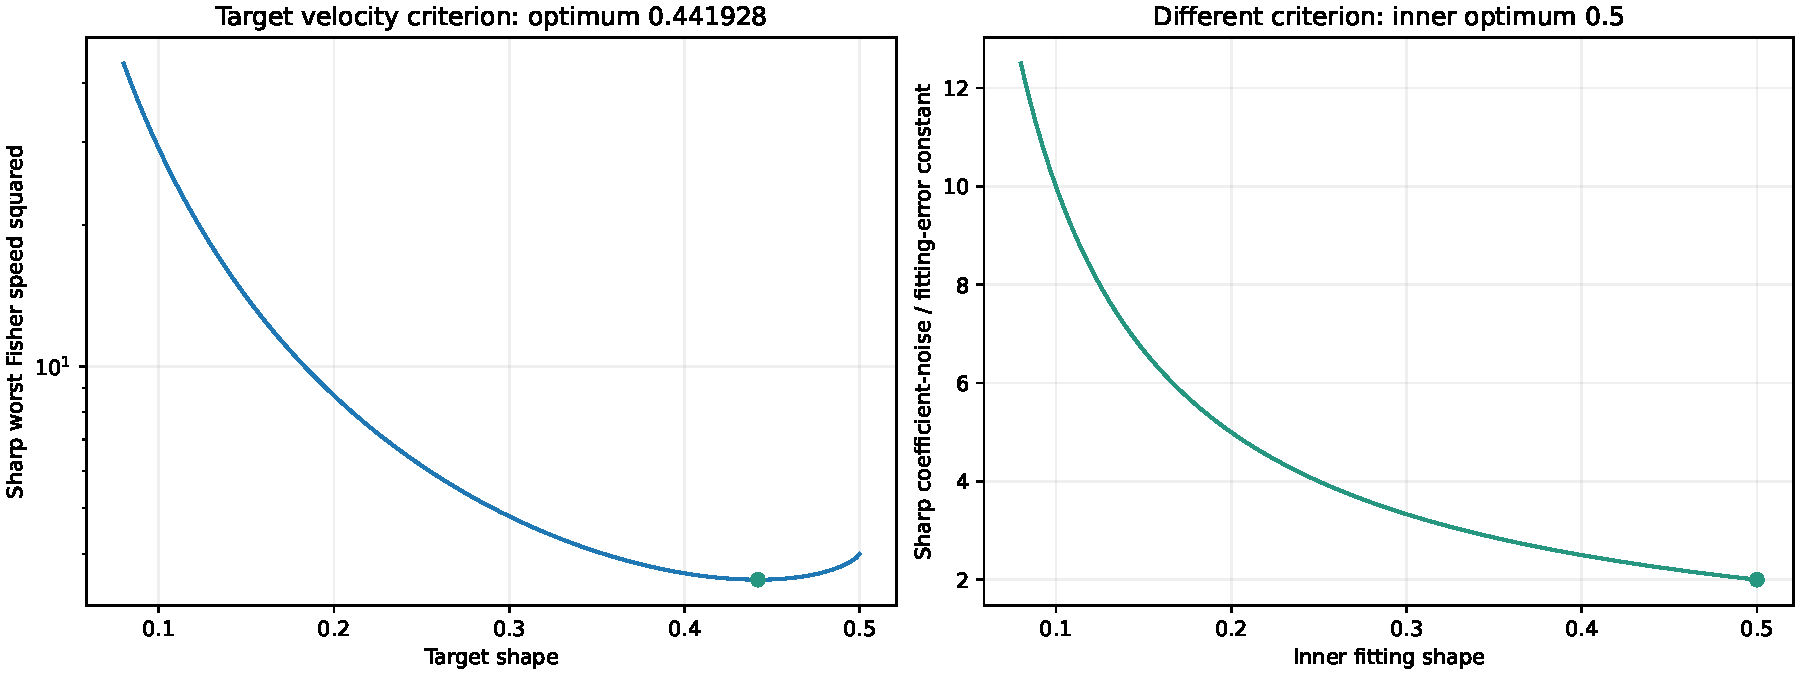
\includegraphics[width=\textwidth]{../../results/power-mean-20261013/two-minimax-criteria.pdf}
 \caption{两个不同的极小极大标准。左图是 target 速度的锐上界，最小点为 $0.441928$；右图是第~\ref{sec:power-projection}~节其他拟合目标的噪声与损失锐相对常数 $1/\kappa_{\mathrm{fit}}$，最小点为 $1/2$。二者都不直接等于最高任务准确率。}
\end{figure}

\subsection{教师误差归一化的锐噪声常数}

\begin{theorem}[平方根形状的相对误差噪声最优性]
\label{thm:power-relative-noise-optimum}
固定 $0<\kappa\le1/2$。令 $\rho=T/q$，小步教师监督为 $A_\kappa^0=(\rho^\kappa-1)/\kappa$，中心为 $K_\kappa^0=[1-\E_q\rho^\kappa]/\kappa$。对至少二元、严格正且 $q\ne T$ 的分布取上确界，有
\begin{align}
 \sup_{q,T}\frac{\Var_qA_\kappa^0}{D_\kappa(T\Vert q)}&=\frac1\kappa,\\
 \sup_{q,T}\frac{\Var_qA_\kappa^0}{K_\kappa^0}&=\frac1{\kappa(1-\kappa)}.
 \label{eq:power-relative-noise-sharp}
\end{align}
在 $\kappa\in[0,1]$ 的幂散度族内，两个准则都由 $\kappa=1/2$ 唯一最小化，锐常数分别为 2 和 4。端点零与 $\kappa>1/2$ 没有有限的统一相对误差常数。
\end{theorem}

\begin{proof}
第~\ref{thm:center-advantage-variance}~定理证明了 $\Var_q(\rho^\kappa)\le[1-a_\kappa]/(1-\kappa)$。除以 $\kappa^2$，再使用 $D_\kappa=[1-a_\kappa]/[\kappa(1-\kappa)]$ 与 $K_\kappa^0=[1-a_\kappa]/\kappa$，得到两个上界。

取 $q=(v,1-v)$、$T=(v^2,1-v^2)$，$v\to0$，则 $\rho=(v,1+v)$。对固定 $0<\kappa\le1/2$，
\begin{equation}
 a_\kappa=v^{1+\kappa}+(1-v)(1+v)^\kappa
 =1-(1-\kappa)v+o(v).
\end{equation}
同理 $a_{2\kappa}=1-(1-2\kappa)v+o(v)$，于是
\begin{equation}
 \Var_qA_\kappa^0=v/\kappa^2+o(v),\quad
 D_\kappa=v/\kappa+o(v),\quad
 K_\kappa^0=(1-\kappa)v/\kappa+o(v).
\end{equation}
相除逼近两个上界，证明锐性。两个常数在 $(0,1/2]$ 上严格递减，最小值均在 $1/2$。

若 $1/2<\kappa<1$，取 $q=(v,1-v)$、$T=(1/2,1/2)$，监督方差按 $v^{1-2\kappa}$ 发散，而 $D_\kappa$ 和 $K_\kappa^0$ 有统一上界。$\kappa=1$ 时方差按 $1/v$ 增长，forward KL 只按 $\log(1/v)$ 增长，且 $K_1^0=0$。$\kappa=0$ 时固定非对称正 $q$，使一个教师概率趋零，方差按平方 log 增长，reverse KL 只按一次 log 增长。故其余形状不存在有限统一常数。
\end{proof}

这个最优性比较的是误差相关噪声常数，并非绝对噪声常数 $C_{\mathrm{vel}}$。所有 $D_\kappa$ 已采用同一局部 Fisher 规范化；其全局值仍随 $\kappa$ 改变。平方根使噪声相对于自身教师误差的最坏放大最小，不意味着每个输入上的方差或任务正确率都最优。

% END SOURCE: sections/proximal_shape_criteria.tex


% BEGIN SOURCE: book/sections/proximal_half_conclusions.tex
\subsection{平方根中间分布的有限步 Hellinger 进展}

平方根 target 把冻结学生与教师的平方根概率加权后归一化，而不是直接对概率作算术平均。记 $u=\sqrt q$、$v=\sqrt T$、$a=u^\top v$、$w=1-\eta$，则
\begin{equation}
 \sqrt{m_{1/2,\eta}}=\frac{wu+\eta v}{\sqrt Z},\qquad
 Z=w^2+\eta^2+2w\eta a.
 \label{eq:power-half-normalized-chord}
\end{equation}
$u,v$ 在正单位球面上。归一化的正线性组合位于两者张成的二维平面及短圆弧上，因而是 Fisher--Rao 路径的一个参数化；$\eta$ 通常不是弧长比例。对 $q=T$，该路径恒定。

\begin{theorem}[平方根 target 的精确亲和度与收缩]
\label{thm:power-half-discrete-contraction}
采用不带 $1/2$ 因子的 $H^2(q,T)=\sum_a(\sqrt{q_a}-\sqrt{T_a})^2=2(1-a)$。精确平方根更新满足
\begin{align}
 a^+&=\sum_a\sqrt{m_aT_a}=\frac{wa+\eta}{\sqrt Z},\\
 H^2(m,T)&\le(1-\eta)H^2(q,T).
 \label{eq:power-half-discrete-progress}
\end{align}
因此固定教师下反复精确更新得到 $H^2(q_N,T)\le(1-\eta)^NH^2(q_0,T)$。目标与锚点的平方根夹角 $\vartheta_{qm}$ 还满足
\begin{equation}
 \cos\vartheta_{qm}=\frac{w+\eta a}{\sqrt Z},\qquad
 \sin^2\vartheta_{qm}=\frac{\eta^2(1-a^2)}Z.
\end{equation}
这些都是精确分布更新的性质，不要求对 teacher 概率指定统一下界。
\end{theorem}

\begin{proof}
式~\eqref{eq:power-half-normalized-chord} 与 $v$ 内积直接给出 $a^+$。由于 $a\le1$，$Z\le(w+\eta)^2=1$，且 $wa+\eta>0$，有 $a^+\ge wa+\eta$。所以 $1-a^+\le w(1-a)$，乘以二即得 Hellinger 收缩。每轮重复应用即可得 $N$ 步界。与 $u$ 内积得到第二个夹角的余弦；再计算 $Z-(w+\eta a)^2=\eta^2(1-a^2)$，得到正弦平方。
\end{proof}

几何端点在同一 Hellinger 指标下没有严格小于一的分布无关单步收缩因子。固定 $0<\eta<1$，取 $q_\epsilon=(\epsilon,1-\epsilon)$、$T=(1/2,1/2)$，则几何 target 的第一坐标为
\begin{equation}
 m_{0,\eta,1}
 =\frac{\epsilon^{1-\eta}}{\epsilon^{1-\eta}+(1-\epsilon)^{1-\eta}}
 \longrightarrow0.
\end{equation}
因此 $q_\epsilon$ 与其几何 target 都趋于 $(0,1)$，两者到 $T$ 的 $H^2$ 都趋于 $2(1-1/\sqrt2)>0$，收缩比趋于一。平方根点的 $(1-\eta)$ 因子加强了相对于几何端点的统一全局 Hellinger 保证；教师附近的局部因子仍与其他形状相同，见后一定理。

\begin{corollary}[平方根精确外层的几何噪声界]
\label{cor:power-half-geometric-noise}
固定教师和 $0<\eta<1$，反复执行精确平方根 target。令 $V_n=\Var_{q_n}A_{1/2,\eta}(T/q_n)$，则
\begin{align}
 V_n&\le\frac{4H^2(q_n,T)}{(1-\eta)^2}
 \le\frac{4(1-\eta)^nH^2(q_0,T)}{(1-\eta)^2},\\
 \sum_{n=0}^\infty V_n&\le\frac{4H^2(q_0,T)}{\eta(1-\eta)^2}
 \le\frac8{\eta(1-\eta)^2}.
\end{align}
若 score 范数统一不超过 $S$，中心化教师梯度的协方差 trace 满足相应右侧乘以 $S^2$ 的界。
\end{corollary}

\begin{proof}
第~\ref{thm:center-advantage-variance}~定理给出 $V_n\le D_{1/2}(T\Vert q_n)/[(1/2)(1-\eta)^2]$。用 $D_{1/2}=2H^2$ 与前一定理的 Hellinger 收缩得到第一式。对 $n\ge0$ 求和，几何级数为 $1/\eta$；最后使用 $H^2\le2$。梯度二阶矩由 score 范数界控制。
\end{proof}

这比一般 MD 的 $O(1/N)$ 监督方差界更明确：平方根精确外层具有同一有界误差量驱动的几何噪声上界，累计上界不依赖可能任意大的初始 KL。它仍要求固定前缀和精确 target 更新；实际 BPO 误差会另外进入进展界。

\begin{figure}[H]
 \centering
 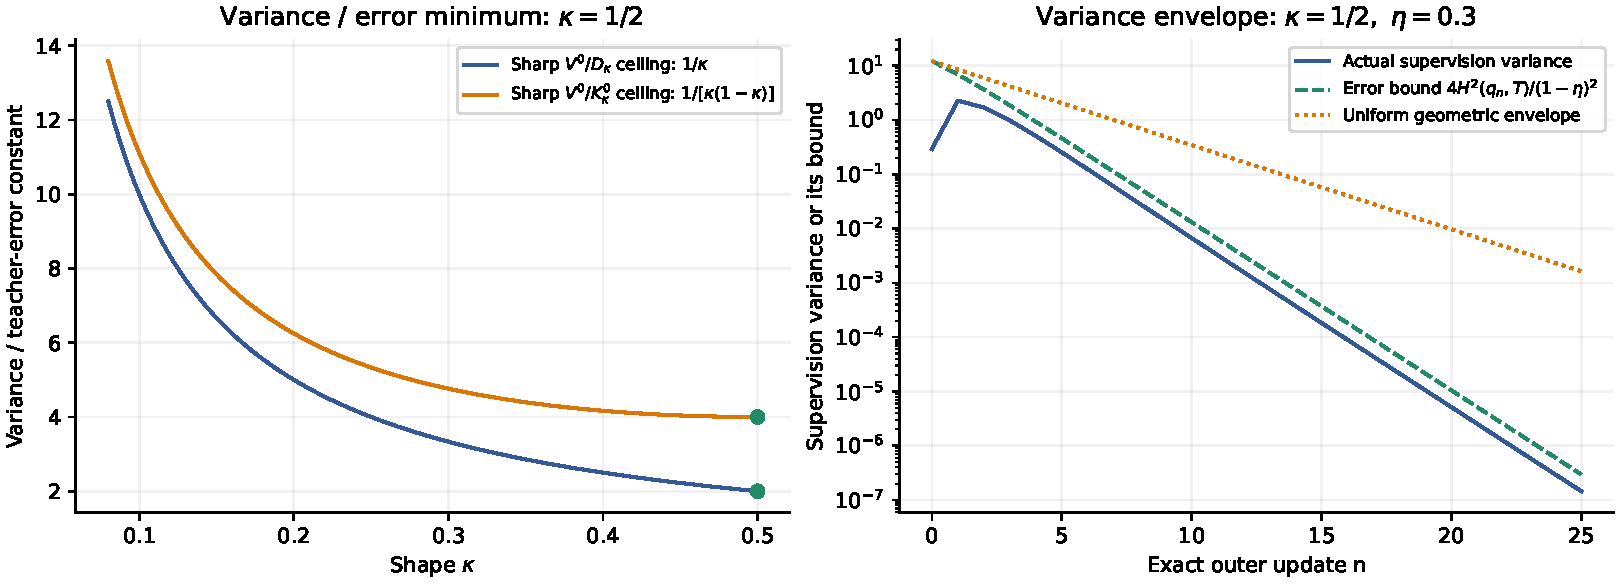
\includegraphics[width=\textwidth]{../../results/chapter9-restructure/relative-noise-and-convergence.pdf}
 \caption{左图以相对教师误差的锐噪声常数选择形状，两个准则均在 $\kappa=1/2$ 最小。右图对 $q_0=(0.999,0.001)$、$T=(0.05,0.95)$、$\eta=0.3$ 做精确平方根迭代。Hellinger 驱动的方差上界和统一几何包络下降，实际标量方差在第一步却增大。几何包络控制收敛过程，并不保证实际方差逐步单调。}
 \label{fig:power-relative-noise-convergence}
\end{figure}

\subsection{所有形状共享局部收敛率}

\begin{theorem}[幂均值的局部展开与共同收缩因子]
\label{thm:power-common-local-rate}
固定正支持教师 $T$、$0<\eta<1$、$0\le\kappa\le1$。令 $q=T+\epsilon h$，其中 $\sum h_a=0$、$h\ne0$，并使全部 $\epsilon h_a/T_a$ 一致趋零。记 $w=1-\eta$、$S_h=\sum_ah_a^2/T_a$，则
\begin{equation}
 m_a=T_a+w\epsilon h_a
 +\frac{(\kappa-1)w\eta}{2}\epsilon^2
       \left(\frac{h_a^2}{T_a}-T_aS_h\right)+O(\epsilon^3).
 \label{eq:power-second-order-target}
\end{equation}
若凸生成函数 $g$ 在一附近三阶可微且 $g''(1)>0$，则
\begin{equation}
 \frac{D_g(m\Vert T)}{D_g(q\Vert T)}
 =(1-\eta)^2+O(\epsilon).
 \label{eq:power-local-divergence-rate}
\end{equation}
因此在同一局部评价散度下，平方根形状没有优于其他形状的一阶概率误差收缩率。固定 $q,\eta$ 的 BPO logits Hessian 同样不因 $\kappa$ 改善。
\end{theorem}

\begin{proof}
对 $\kappa>0$，先展开
\begin{equation}
 (1-\eta)q_a^\kappa+\eta T_a^\kappa
 =T_a^\kappa\left[1+w\kappa\epsilon\frac{h_a}{T_a}
 +\frac{w\kappa(\kappa-1)}2\epsilon^2\frac{h_a^2}{T_a^2}
 +O(\epsilon^3)\right].
\end{equation}
再使用 $(1+x)^{1/\kappa}$ 的二阶展开，未归一化幂均值为
\begin{equation}
 \widetilde m_a=T_a+w\epsilon h_a
 +\frac{(\kappa-1)w\eta}{2}\epsilon^2\frac{h_a^2}{T_a}+O(\epsilon^3).
\end{equation}
求和时一次项消失，得到 $Z=1+[(\kappa-1)w\eta/2]\epsilon^2S_h+O(\epsilon^3)$。除以 $Z$ 即得第一式。几何端点可以直接展开 $q_a^wT_a^\eta$，得到同一式子中 $\kappa=0$ 的结果。

将 $g$ 加上线性项使 $g'(1)=0$ 不改变散度。Taylor 展开给出 $D_g(q\Vert T)=g''(1)\epsilon^2S_h/2+O(\epsilon^3)$。用 $m-T=w\epsilon h+O(\epsilon^2)$ 再展开，得到 $D_g(m\Vert T)=g''(1)w^2\epsilon^2S_h/2+O(\epsilon^3)$。$g''(1)S_h>0$，相除得到第二式。BPO 的曲率结论由第~\ref{sec:power-bpo-algorithm}~节的精确二次型给出。
\end{proof}

\subsection{形状选择取决于明确的评价标准}

\begin{center}
\small
\begin{tabular}{p{55mm}p{35mm}p{54mm}}
\toprule
评价标准 & 结论 & 条件与含义\\
\midrule
小步监督的分布无关有限方差 & $0<\kappa\le1/2$ & $1/2$ 是该区间的最大形状\\
小步方差相对教师误差的最坏比值 & $\kappa=1/2$ & $V\le2D_{1/2}=4H^2$，常数最优\\
最坏小步标量方差／Fisher 速度 & $\kappa_\star\simeq0.441928$ & 锐值 $3.527275$；平方根为 4\\
相同 Fisher 速度下的 reverse KL 局部下降 & $\kappa=0$ & 最陡确定性方向；无统一尾部界\\
相同 Fisher 速度下的 forward KL 局部下降 & $\kappa=1$ & 最陡确定性方向；小步最坏方差发散\\
当前学生采样的幂散度拟合噪声常数 & $\kappa_{\mathrm{fit}}=1/2$ & 拟合形状的最优性，不是 BPO target 最优性\\
固定 $q,\eta$ 的 BPO 条件数 & 对所有 $\kappa$ 相同 & 形状只改变 target 与初始残差\\
数学任务正确率与 NN 优化效率 & 尚无普遍最优点 & 不能用上述单一常数替代任务指标\\
\bottomrule
\end{tabular}
\end{center}

平方根点具有一个简洁的组合：球面中间 target、统一小步方差界、Hellinger 误差相关噪声和显式精确外层收缩。$\kappa_\star$ 则针对另一个明确准则将最坏小步标量方差上界从 4 降到约 3.5273。较小的方差常数同时可能缩小某些方向的信号；它不等于更高的梯度信噪比或更快的任务学习。

这些比较保持了同一个局部监督尺度：对所有形状，$A'_{\kappa,\eta}(1)=1$，等价于 $\partial_r f_{\kappa,\eta}(0)=\eta$。教师目标的生成函数也均满足 $\omega''_{\kappa,\eta}(1)=1$。形状改变的是远离教师时的路径和尾部响应；其小步方差差异没有通过一个额外的整体信号缩放制造。

有限步的共同 teacher 误差也没有统一的形状排序。固定 $\eta=0.3$，取 $q=(0.9,0.1)$、$T=(0.01,0.99)$，几何 target 的 Hellinger 误差低于平方根 target；改为 $q=(0.99,0.01)$、$T=(0.5,0.5)$，平方根 target 的 Hellinger 误差低于几何 target。两对输入都严格为正，直接代入闭式 target 即可验证。

\begin{figure}[H]
 \centering
 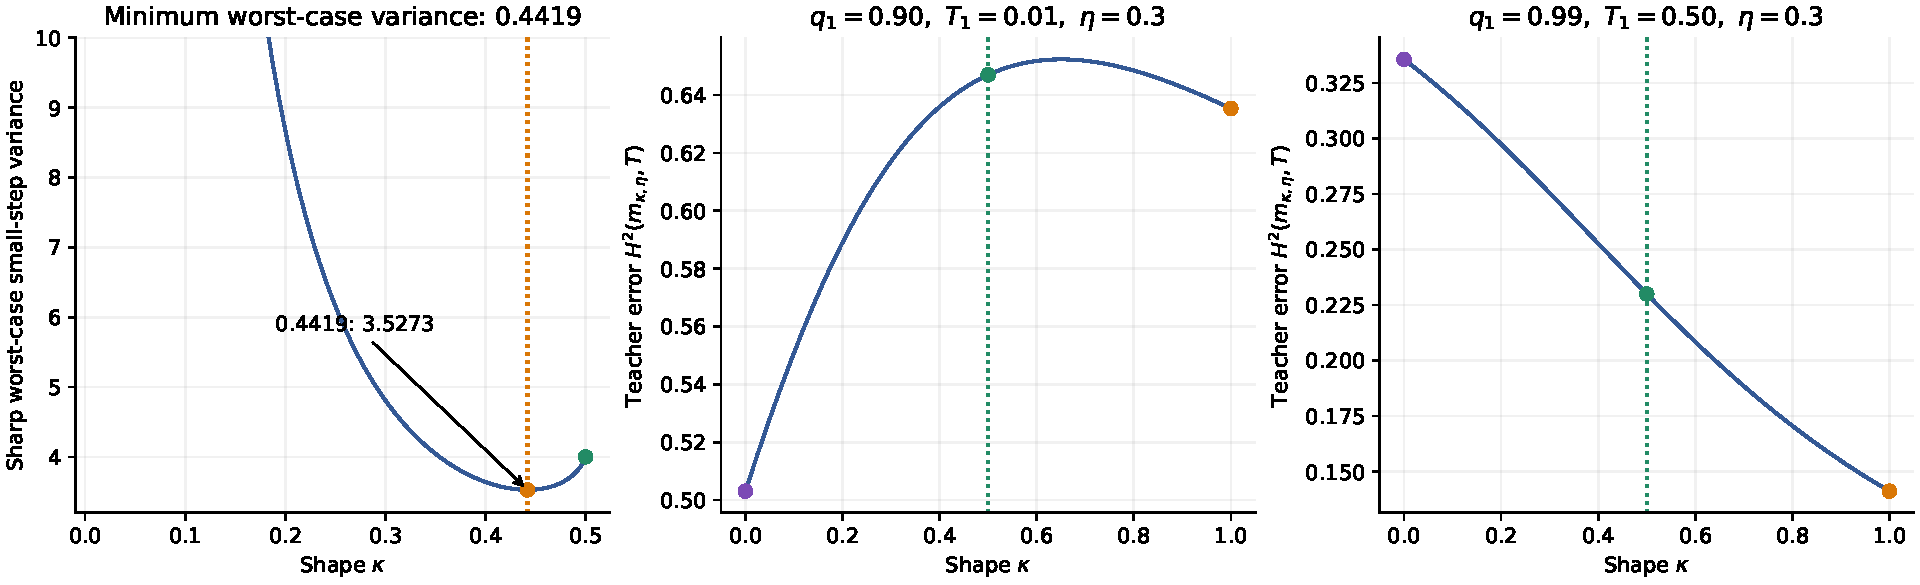
\includegraphics[width=\textwidth]{../../results/chapter9-restructure/kappa-criteria.pdf}
 \caption{形状的优势取决于评价标准。左图为锐最坏小步方差常数，最小点约为 $0.4419$，平方根点为 4。中、右图对同一 $\eta=0.3$ 使用两对固定二元分布，比较精确 target 后的同一 Hellinger 误差；曲线没有一致的形状排名。图只计算解析概率公式，不使用模型训练。}
 \label{fig:power-kappa-criteria}
\end{figure}

学生和教师的加权分布还可以用作辅助 action 提案，例如 $\mu_\zeta=(1-\zeta)q+\zeta T$。这与平方根监督 target 是两个选择：前者通过重要性校正估计原 $q$ 加权 BPO 损失，后者改变要拟合的目标。提案混合能控制重要性比率并在一些稀有 action 输入上改善相对方差，但没有每个输入都降低方差的保证。第~\ref{sec:power-estimators}~节给出无偏性、反例和排除重复 action 后的协方差半正定改进。

% END SOURCE: sections/proximal_half_conclusions.tex


\section{中心估计与单轨迹的 action 估计}
\label{sec:power-estimators}
\label{sec:center-extensions}

% BEGIN SOURCE: book/sections/proximal_center_estimators.tex
\subsection{精确求和、Monte Carlo 与非负估计的代价}

若 teacher forward 能提供该前缀完整 logits，则使用完整 $q$ 权重直接求式~\eqref{eq:center-expanded-k}，不需要生成第二条 response。信号在 log 空间用 logaddexp 计算，避免先形成极大的 $T/q$。该中心可以按 prefix 缓存并冻结。

若采用独立 $a_i\sim q(\cdot\mid s)$，有无偏估计
\begin{equation}
 \widehat K=-\frac1M\sum_{i=1}^MA(a_i),\qquad
 \Var\widehat K=V/M.
\end{equation}
$\widehat K$ 单次可以为负；这不违背其非负期望。另一个逐样本非负无偏估计为
\begin{equation}
 \widehat K_+=\frac1M\sum_i[\rho(a_i)-1-A(a_i)].
\end{equation}
两者期望相同，方差一般不同。 它们在局部与最坏尾部上具有不同表现。若 $\rho=1+\epsilon h$、$\E_qh=0$ 且 $h$ 有界，令 $c_0=1-\kappa(1-\eta)$，则
\begin{align}
 -A&=-\epsilon h+\tfrac12c_0\epsilon^2h^2+O(\epsilon^3),\\
 \phi(\rho)&=\tfrac12c_0\epsilon^2h^2+O(\epsilon^3),\\
 \Var(-A)&=\epsilon^2\E_qh^2+O(\epsilon^3),\\
 \Var\phi(\rho)&=\tfrac14c_0^2\epsilon^4\Var_q(h^2)+O(\epsilon^5).
\end{align}
因此包括 $\kappa=0$ 在内，接近同分布时非负控制变量估计可把方差从二阶降至四阶；这需要概率比一致接近一，不能扩展到任意重尾输入。

取 $q=(\epsilon,1-\epsilon)$、$T=(1/2,1/2)$、固定 $\kappa>0,\eta<1$，原始估计方差按 $O(\epsilon\log^2(1/\epsilon))\to0$；非负估计的稀有项为 $\rho\sim1/(2\epsilon)$，其方差按 $1/(4\epsilon)$ 发散。这个 $\rho-1$ 控制变量保证非负性，却不能提供统一低方差保证。固定数据上也可能降低方差，应记录真实条件矩后判断。 即便原 KL 很小，也不能自动使用局部结论：取 $q=(\epsilon,1-\epsilon)$、$T=(\epsilon^{1/4},1-\epsilon^{1/4})$，有 $\KL(q\Vert T)\sim\epsilon^{1/4}\to0$，但非负估计的方差按 $\epsilon^{-1/2}$ 发散。概率比一致接近一比 KL 小更强。

如果独立中心估计与当前 action 独立，$\Var[A(a)+\widehat K]=V+V/M$。估计中心不会自动降低标量 advantage 方差。若中心与 advantage 使用同一组 $M$ 个 action，固定参数下
\begin{equation}
 \E\left[\frac1M\sum_i(A_i-\bar A)\psi_i\right]
 =\frac{M-1}{M}\operatorname{Cov}_q(A,\psi).
\end{equation}
这个恒等式由展开双重和得到：$M$ 个同索引项贡献 $\E A\psi$，$M(M-1)$ 个异索引项贡献 $\E A\E\psi$。$M=1$ 时更新为零。 若同一个 action 改用非负估计 $\widehat K_+=\rho-1-A$，则
\begin{equation}
 A(a)+\widehat K_+(a)=\rho_a-1,
\end{equation}
完全消掉 $\kappa,\eta$ 的教师信号形状。在 $p=q$ 时，该 score 更新的期望是 $\E_T\psi_q$，对应 forward-KL 的下降方向，而不是原 $\E_qB\psi_q$。中心估计本身无偏，不代表与当前 action 共享样本后的梯度无偏。

$M>1$ 可以使用独立中心、leave-one-out 或无偏样本协方差系数；它们要求同一 prefix 下的独立动作，不能用不同前缀的 token 直接代替。本研究的主 BPO 路线采用完整条件求和，不引入 response 组。
\subsection{有界非负无偏中心估计器}

$q$ 提案下的非负估计会出现重尾，但可以利用已有 $K$ 上界构造另一个提案。令 $\kappa>0,\eta<1$，$c=-\log(1-\eta)/(\kappa\eta)\ge1$。由 $A\ge-c$ 与 $\phi\ge0$，逐 action 有
\begin{equation}
 0\le q_a\phi(\rho_a)\le T_a+(c-1)q_a.
\end{equation}
右侧的总质量是 $c$，所以定义归一化包络提案
\begin{equation}
 \mu_c=(1-1/c)q+(1/c)T,\qquad
 Z(a)=\frac{q_a}{\mu_c(a)}\phi(\rho_a),\quad a\sim\mu_c.
 \label{eq:center-bounded-mixture-estimator}
\end{equation}
无需知道真实 $K$ 即可采样：以概率 $1/c$ 从教师抽一个 action，否则从锚点抽一个 action。它只估计本 prefix 的中心，不把 response rollout 改为这个提案，也不引入 response 组。

\begin{theorem}[中心估计的最小统一样本上界]
\label{thm:center-bounded-estimator}
上述估计器满足
\begin{equation}
 \E_{\mu_c}Z=K,\qquad0\le Z\le c,\qquad
 \Var_{\mu_c}Z\le K(c-K)\le c^2/4.
\end{equation}
对 $M$ 次独立抽样，$\widehat K_\mu=M^{-1}\sum_iZ_i$ 无偏、非负且不超过 $c$，其方差不超过 $K(c-K)/M$。所有分布上统一成立的无偏估计器样本上界不可能小于 $c$。
\end{theorem}

\begin{proof}
定义给出 $\E_\mu Z=\sum_aq_a\phi(\rho_a)=K$。包络不等式给出 $0\le Z\le c$，于是 $Z^2\le cZ$，取期望再减 $K^2$ 得到方差界。独立平均将方差除以 $M$。若任意无偏估计器总被常数 $b$ 上界约束，则 $K=\E\widehat K\le b$；而前面的正支持见证可以使 $K\to c$，故 $b\ge c$。这个最优性只作用于统一样本上界，不宣称该提案在每个固定分布上具有最小方差。\hfill$\square$
\end{proof}

Hoeffding 不等式还给出明确的置信界
\begin{equation}
 \Pr\{ |\widehat K_\mu-K|\ge\epsilon\}
 \le2\exp(-2M\epsilon^2/c^2).
\end{equation}
$\kappa=0$ 或 $\eta=1$ 的 KL 在分布类上无界，因此不能保持一个有限统一样本上界的无偏估计器。固定已知分布可以有有限界，不能与这个分布类结论混同。

平方根的小步极限尤为直观：$c\to2$、$\mu_c\to(q+T)/2$、$\phi(\rho)\to(\sqrt\rho-1)^2$，于是
\begin{equation}
 Z_0(a)=\frac{2(\sqrt{T_a}-\sqrt{q_a})^2}{T_a+q_a}\in[0,2],
 \qquad\E_{(q+T)/2}Z_0=H^2(q,T).
\end{equation}
记 $K_{\mathrm H}=H^2$，则 $\Var Z_0\le K_{\mathrm H}(2-K_{\mathrm H})$；而 $q$ 提案下的原始有符号中心估计在此极限具有方差 $K_{\mathrm H}(4-K_{\mathrm H})$。因此在每个固定完整支持分布对的平方根小步极限，包络估计方差至多为原始估计的一半。有限 $\eta$ 时不保证逐输入都优于原始有符号估计，真实条件矩仍需报告。 若当前 $q$ action 与 $M$ 个中心样本独立，则估计 advantage $\widehat B=A(a)+\widehat K_\mu$ 的方差为 $V+\Var Z/M$。平方根小步极限因此满足
\begin{align}
 \Var\widehat B
 &\le K_{\mathrm H}(4-K_{\mathrm H})
    +K_{\mathrm H}(2-K_{\mathrm H})/M\\
 &\le4+\frac1{M(M+1)}.
\end{align}
第二步在 $K_{\mathrm H}\in[0,2]$ 上最大化该凹二次式，驻点为 $(2M+1)/(M+1)$。一个独立辅助中心 action 即 $M=1$ 时，上界为 4.5；使用有符号 $q$ 中心估计的对应统一界为 8。这个结论作用于冻结 prefix 的教师标量 advantage，并要求独立性；它不涵盖学生反馈项或直接成为全参数梯度方差定理。


主 BPO 的完整条件求和无需这个辅助估计器。若使用它构造 sampled-action advantage，中心抽样仍须与当前 action 独立，或者给出相关性修正；有界中心估计不使 $A$ 的正尾部变为有界，也不自动解决整段 inner 的缓存误差。单样本中心只需本前缀辅助 action，不能把它解释为新增完整 response。
\subsection{有限 head 与尾部质量的中心区间}

令 $S$ 为任一保留 head，$\delta=\sum_{a\notin S}q_a$、$\tau_T=\sum_{a\notin S}T_a$，记 $K_S=-\sum_{a\in S}q_aA_a$。当 $\delta>0$，尾部的 $\rho$ 条件均值为 $\tau_T/\delta$。函数 $-A(\rho)$ 凸且不超过 $c$，由 Jensen 得到
\begin{equation}
 \boxed{K_S-\delta A(\tau_T/\delta)
 \le K\le K_S+\delta c_{\kappa,\eta}.}
 \label{eq:center-head-tail-interval}
\end{equation}
下界正是把尾部合并为一个 action 后的中心，亦为对应 $f$-divergence 的数据处理下界。区间宽度为 $\delta[c+A(\tau_T/\delta)]$，可直接计算；$\delta=0$ 时直接用完整 head 和。几何端点仍有 Jensen 下界，但没有仅靠两种尾部质量获得的有限统一上界。 对嵌套 head，拆分尾部由 Jensen 保证下界非减少；新增 action $a$ 对上界的改变量为 $q_a[-A_a-c]\le0$，所以上界非增加。可以持续扩大 head，直到区间宽度不超过 $\epsilon$，再取中点获得绝对中心误差不超过 $\epsilon/2$ 的确定性证书。

以一个已估计中心代替精确 $K$，会给 BPO score 系数加入常数误差 $\Delta K$。若 $\Delta K=\widehat K-K$，当前学生不等于 $q$ 时，梯度偏差为 $-\Delta K\E_q\psi_p$，若 $\|\psi_p\|\le S$，其范数不超过 $S|\Delta K|$。因此区间既报告中心误差，也能给固定参数下的 score 偏差提供证书。 这个偏差结论作用于停止系数并使用原始 $\psi_p$ 的 score 更新。若精确微分学生条件中心，情况不同：固定的教师中心误差使完整平方损失仅增加 $\eta(\Delta K)^2/2$，不改变其梯度。对应无偏形式是
\begin{equation}
 g_{\mathrm{cscore}}=
 [C_qU/\eta-A-\widehat K]\,[\psi_p-\E_q\psi_p].
\end{equation}
对于固定参数、精确学生中心和不依赖当前 action 的任意冻结 $\widehat K$，其 $q$ 期望等于真实 BPO 梯度。也可以通过停止系数乘以 $\log p(a)-\E_q\log p$ 实现这个梯度；教师中心于是只影响该估计器的方差；若其误差不消失，在 $p=m$ 处仍可能保留采样噪声，不能自动继承精确残差估计器的零噪声性质。若中心来自当前 action，或学生中心也只是有偏近似，则不能直接套用这项结论。
\subsection{标量中心不等于最优梯度 baseline}

在 inner 起点 $p=q$，$\E_q\psi_q=0$，任意常数 baseline 都保持教师 score 梯度期望。令 $w(a)=\|\psi_q(a)\|^2$，则使协方差 trace 最小的 baseline 为
\begin{equation}
 b_\star=\frac{\E_q[A w]}{\E_qw},\qquad
 V_g(b)=\E_q[(A-b)^2w]-\|\E_qA\psi_q\|^2.
\end{equation}
配方平方给出
\begin{equation}
 V_g(\E_qA)-V_g(b_\star)
 =\E_qw\,(\E_qA-b_\star)^2\ge0.
\end{equation}
因此精确均值中心 $-K$ 不保证梯度方差最小，也不保证优于不使用 baseline。二元 $q=(0.99,0.01)$、$T=(0.5,0.5)$、$\kappa=0.5$、$\eta=0.3$ 下，categorical logit 梯度协方差 trace 从无 baseline 的 0.92622 增至均值 baseline 的 1.07537，而 score 加权最优 baseline 在这个二元例子中给出零方差。

对另一种采用当前学生重要性权重的估计器 $g_b=\omega(f-b)\psi_p$、$\omega=p/q$，$\E_q\omega\psi_p=0$，所以常数 baseline 不改变均值。微分 $\E_q[\omega^2(f-b)^2\|\psi_p\|^2]$ 得到
\begin{equation}
 b_\star^{\mathrm{IS}}
 =\frac{\E_q[\omega^2f\|\psi_p\|^2]}{\E_q[\omega^2\|\psi_p\|^2]}.
\end{equation}
这里的估计测度和重要性权重与 BPO 不同，不能直接替换冻结 $q$ 下的 BPO 中心。

当前 $p\ne q$ 时，$\E_q\psi_p$ 通常非零，不能直接替换 BPO 中心而保持梯度不变。若需要额外调整 residual baseline，须加入相应确定性补偿项。教师 $K$ 是 BPO 目标定义的一部分，最优 score baseline 是估计器的另一个选择。

教师 advantage 的性质主要控制 inner 起点。一般 inner 的净监督是 $B-C_qU/\eta$；学生反馈可能无界。前节的残差二阶矩界 $\E\|g\|^2\le(2S^2/\eta)\mathcal L_{\mathrm{BPO}}$ 仍适用，但不把教师单侧界升级为全训练系数的绝对界。

\begin{figure}[htbp]
 \centering
 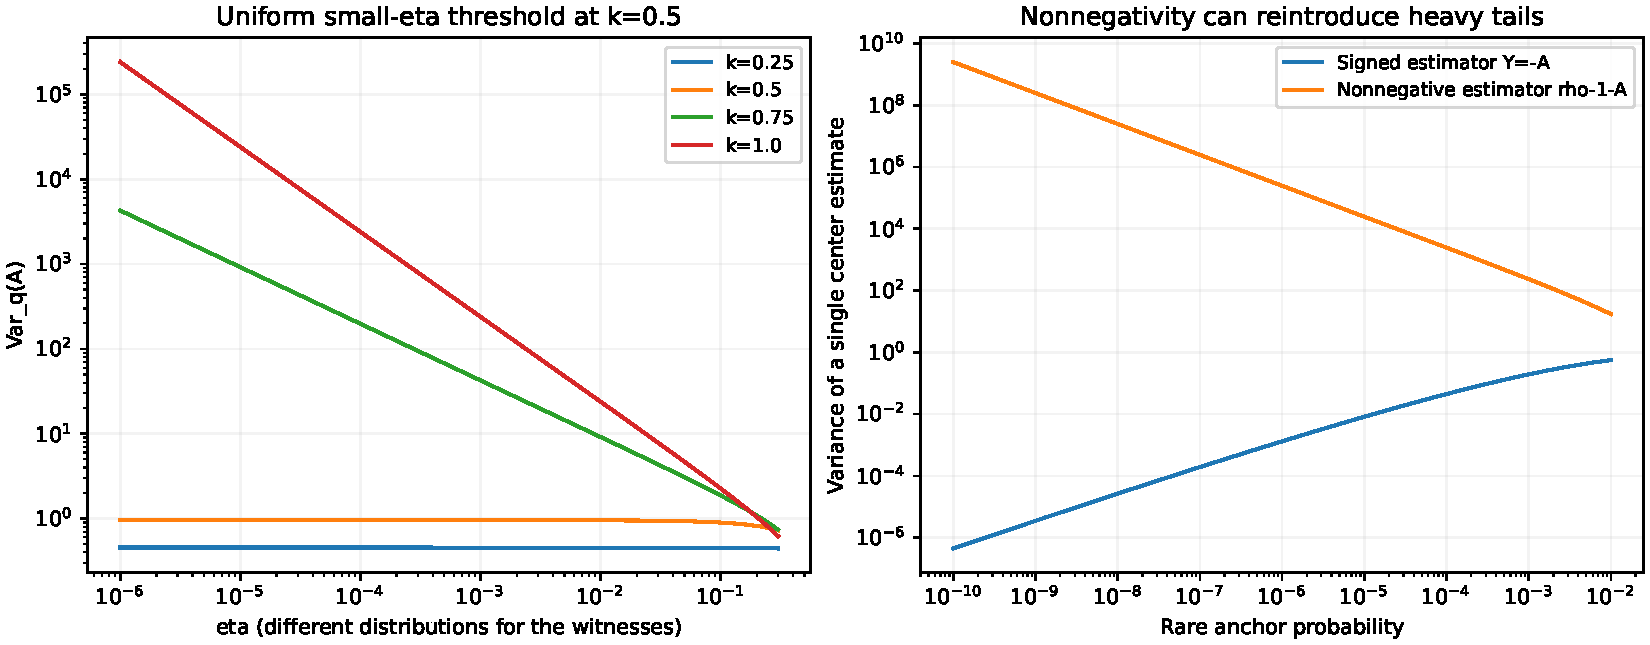
\includegraphics[width=\textwidth]{../../results/power-center-advantage/small-step-and-estimation.pdf}
 \caption{左：小步方差阈值的下界见证，不同形状使用不同分布族，不能当作同数据上的性能排名。右：逐样本非负中心估计可能重新引入概率比重尾。}
\end{figure}
\begin{figure}[htbp]
 \centering
 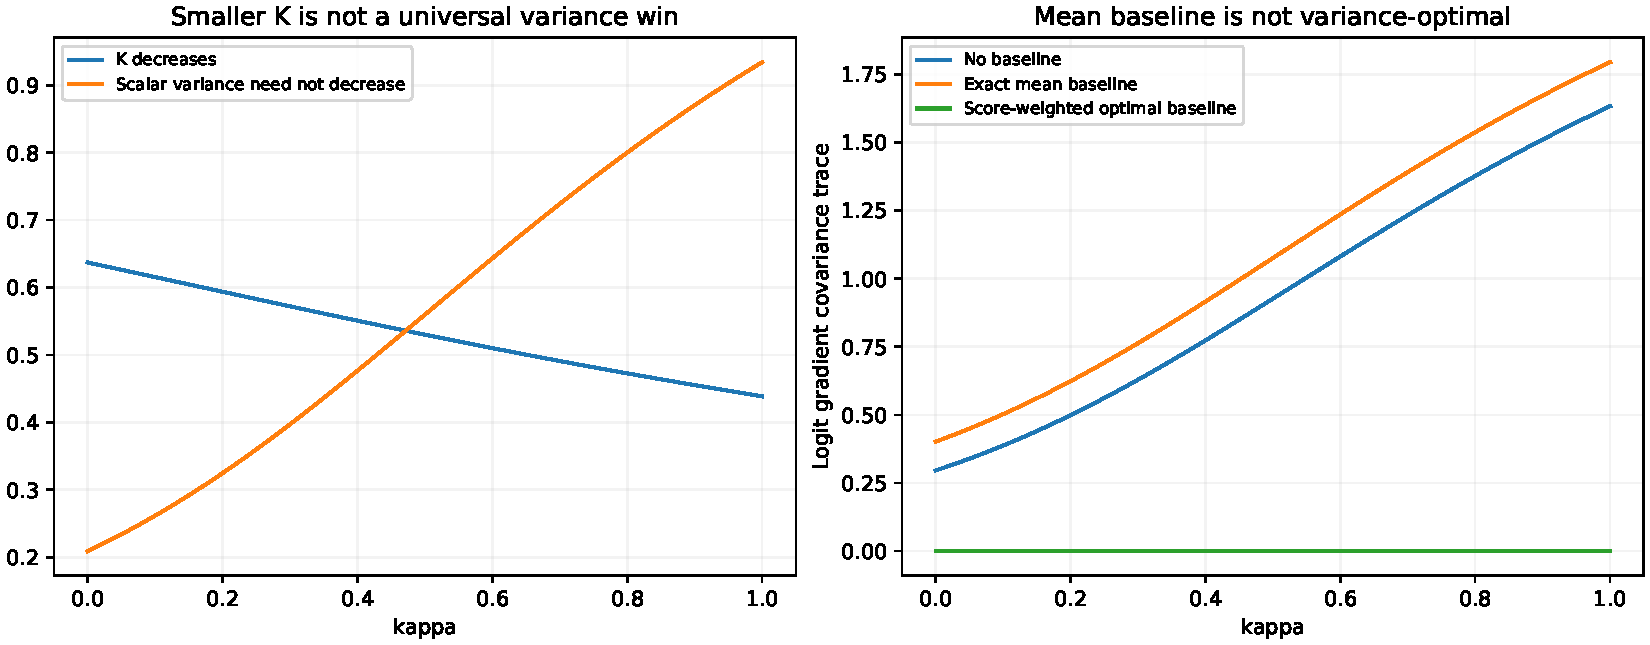
\includegraphics[width=\textwidth]{../../results/power-center-advantage/baseline-counterexample.pdf}
 \caption{同一二元输入下，$K$ 随形状下降但标量方差不必下降；均值 baseline 也不一定降低 logit 梯度方差。零方差最优 baseline 是二元例子的性质，不是一般网络结论。}
\end{figure}

数学核验与真实缓存审计见 \path{experiments/analysis/power_center_advantage.py}；真实缓存取原 64 条 t22 response 每条两个固定随机 reservoir 位置，共 128 个 prefix，对 20 组 $\kappa,\eta$ 精确求 action 条件矩。结果与所有实验统一维护在唯一实验报告；这些 CPU 模型分布统计不等于新 GPU 训练或全参数梯度方差。

% END SOURCE: sections/proximal_center_estimators.tex


% BEGIN SOURCE: book/sections/proximal_center_extensions.tex
下面继续在同一冻结前缀上改进 $K$ 的辅助 action 估计。除专门的 logits 结论外，所有向量方差均指协方差 trace，参数固定，动作来自同一 prefix 的独立条件抽样。辅助 action 不等于新增完整 response；对不同 prefix 的 token 套用本节协方差公式会改变目标。

\subsection{一般混合提案的样本上界与输入方差最优性}

记 $\rho=T/q$、$\phi=\rho-1-A$、$c=-\log(1-\eta)/(\kappa\eta)$，这里 $\kappa>0$、$\eta<1$，所以 $c>1$。对任意 $0<\zeta<1$，取 $\mu_\zeta=(1-\zeta)q+\zeta T$、$Z_\zeta=\phi/(1-\zeta+\zeta\rho)$。它对 $K$ 无偏。由 $0\le\phi(x)\le x+c-1$，
\begin{equation}
 0\le Z_\zeta\le C_\zeta,
 \qquad C_\zeta=\max\{(c-1)/(1-\zeta),1/\zeta\}.
\end{equation}
这个上界是逐概率比的精确上确界：$x\to0$ 时 $\phi(x)\to c-1$；$x\to\infty$ 时 $\phi(x)/x\to1$，两个端点分别达到上述两项。第一项随 $\zeta$ 增加、第二项随 $\zeta$ 减少，唯一最小最大值发生在 $\zeta=1/c$，值为 $c$。这解释前节提案的选择，不表示其每个输入的方差最小。

固定输入的方差为
\begin{equation}
 W(\zeta)=\E_q\frac{\phi(\rho)^2}{1+\zeta(\rho-1)}-K^2,
 \qquad W''(\zeta)=2\E_q\frac{\phi(\rho)^2(\rho-1)^2}{[1+\zeta(\rho-1)]^3}\ge0.
\end{equation}
因此可以做一维凸优化选择输入方差最优混合权重；它可以落在端点，也可以不同于 $1/c$。随机 pilot 选权重时，后续样本应与选权重的数据独立，或给出适应性修正。更小的输入方差与更小的统一样本范围是不同目标。
\subsection{把 head--tail 区间变成有界无偏估计器}

令 head 为 $S$、尾部为 $C$，$\delta=\sum_Cq$、$\tau_T=\sum_CT$，假设 $\delta,\tau_T>0$。定义 $r_0=\tau_T/\delta$、$H=\sum_Sq\phi(\rho)$。上一小节的确定性区间可改写为
\begin{align}
 L&=H+\delta\phi(r_0),\\
 U&=H+\tau_T+(c-1)\delta,\\
 w&=U-L=\delta[c+A(r_0)].
 \label{eq:center-tail-interval-lu}
\end{align}
我们可以使随机估计值始终位于这个区间，同时保持无偏。

对尾部概率比定义凸余项
\begin{align}
 g(x)&=\phi(x)-\phi(r_0)-\phi'(r_0)(x-r_0)\\
 &=-A(x)+A(r_0)+A'(r_0)(x-r_0),\\
 u&=A'(r_0)=\frac{r_0^{\kappa-1}}{1-\eta+\eta r_0^\kappa},\qquad
 v=c+A(r_0)-r_0u.
\end{align}
凸性给出 $g\ge0$，且 $A\ge-c$ 给出 $g(x)\le ux+v$。$u>0$；$A$ 凹且 $A(0)=-c$，在 $r_0$ 处的切线于零点的截距 $A(r_0)-r_0A'(r_0)$ 不低于 $-c$，所以 $v\ge0$。尾部中 $\sum_Cq(\rho-r_0)=0$，故
\begin{equation}
 \sum_Cqg(\rho)=K-L,\qquad u\tau_T+v\delta=w.
\end{equation}
当 $w>0$，取仅支持尾部的提案和估计值
\begin{equation}
 \nu(a)=\frac{uT_a+vq_a}{w},\qquad
 Y(a)=\frac{q_ag(\rho_a)}{\nu(a)},\quad a\sim\nu.
\end{equation}
由 $g\le u\rho+v$，有 $0\le Y\le w$。提案可通过条件尾部分布抽样：以概率 $u\tau_T/w$ 从 $T(\cdot\mid C)$ 抽一个 action，否则从 $q(\cdot\mid C)$ 抽一个 action。其响应 rollout 测度仍为 $q$。

\begin{theorem}[区间内的无偏教师中心估计]
\label{thm:center-tail-bounded-estimator}
令 $Y_1,\ldots,Y_M$ 为上述独立尾部样本，$\widehat K=L+M^{-1}\sum_iY_i$。则
\begin{align}
 \E\widehat K&=K,\qquad L\le\widehat K\le U,\\
 \Var\widehat K&\le\frac{(K-L)(U-K)}M\le\frac{w^2}{4M},\\
 \Pr(|\widehat K-K|\ge\epsilon)&\le2\exp(-2M\epsilon^2/w^2).
\end{align}
若 $w=0$ 或尾部为空，直接返回确定的 $K=L=U$。
\end{theorem}

\begin{proof}
尾部余项的恒等式给出 $\E_\nu Y=K-L$，所以均值正确。逐样本范围给出 $Y^2\le wY$，因此 $\Var Y\le w(K-L)-(K-L)^2=(K-L)(U-K)$。独立平均除以 $M$，并用 Hoeffding 得到最后一式。$L\ge0$ 是粗粒化的凸散度，故估计非负。\hfill$\square$
\end{proof}

估计需要能够从条件尾部分布抽样并读取抽中 action 的 $q_a,T_a$。仅有 head 与两种尾部质量时，不能无偏还原 $K$：保持全部已知量不变，让尾部 $T/q$ 恒定得到下界 $L$，将教师尾部质量偏向一个 action 则由严格凸性得到更大的 $K$。仅依赖已知量的随机估计器对两种输入具有相同期望，不能同时无偏。若完整 logits 已经可用，精确求和通常更直接；稀疏缓存模式需把尾部查询成本纳入比较。

无 head 时，$\delta=\tau_T=r_0=1$、$u=1$、$v=c-1$、$L=0$、$w=c$，精确恢复前节全词表包络估计器。扩大嵌套 head 会缩小 $w$，所以最坏方差和置信宽度保证单调改善；不能据此声称实际输入方差也一定单调改善。若允许至少两个未知尾部 action，在固定 head 和尾部质量下可以令尾部 $q$ 质量集中在 $T/q\to0$ 的 action、$T$ 质量集中在极小 $q$ 的另一个 action，使 $K\to U$。任何无偏、非负的残差估计器若有统一样本上界 $b$，都需 $b\ge\sup(K-L)=w$；本构造达到这个信息条件下的统一范围。

还有一个容易实现的备选：直接估计尾部 $\sum_Cq\phi$，使用提案 $(T+(c-1)q)/[\tau_T+(c-1)\delta]$ 在尾部条件化，再加精确 head。固定此包络时，逐步扩大 head 的实际估计方差也不增加：若原提案落入新尾部的概率为 $p_C$，新估计方差为 $p_C^2\Var(Z\mid C)$，原方差由全方差公式至少为 $p_C\Var(Z\mid C)$。但该备选的随机值不保证高于更强的 Jensen 下界 $L$。两种估计分别提供实际方差单调性与更紧的逐样本区间，不混用结论。

% END SOURCE: sections/proximal_center_extensions.tex


% BEGIN SOURCE: book/sections/proximal_action_estimators.tex
\subsection{缓存教师中心误差与末期噪声}

记 $h=U-f$、$R=C_qh$、$D=R/\eta$、$\psi=\nabla\log p$、$\varphi=\psi-\E_q\psi$。真实 BPO 梯度为 $\bm G=\E_qD\psi=\E_qD\varphi$。若缓存 $\widehat K=K+e$，使用未修正的 score 更新会产生偏差 $-e\E_q\psi$。改用中心化 score 后，任意固定 $e$ 都不改变梯度期望，却保留随机性。尤其在 $p=m$，$D=0$，
\begin{equation}
 g=-e\varphi,\qquad
 \Var_q(g)=e^2\E_q\|\varphi\|^2.
\end{equation}
若中心用 $M$ 个独立样本估计、方差为 $\sigma_K^2/M$，再对中心误差求平均，就得到 $\sigma_K^2\E_q\|\varphi\|^2/M$ 的末期噪声。完整条件求和时，$\E_q\varphi=0$ 会精确消掉这一项；因此完整词表 BPO 不需要通过教师中心估计器控制这一采样噪声来源。

可以利用学生反馈估计中心：令 $y=C_qU/\eta-A$，则 $\E_qy=K$，而
\begin{equation}
 \Var_qy=\Var_qD=\frac{2\mathcal L_{\mathrm{BPO}}}{\eta}.
\end{equation}
独立辅助 action 上的 $y$ 估计在拟合到 target 时方差消失，优于仅依靠 teacher 监督的固定中心噪声底；它通常没有逐样本统一范围。下面将这个差分进一步对称化，同时消去学生条件中心。
\subsection{不显式估计两个中心的 BPO 二样本损失}

令 $a,b\overset{\mathrm{iid}}\sim q$，定义
\begin{equation}
 \widehat\ell_2=\frac{[h(a)-h(b)]^2}{4\eta},\qquad
 \widehat{\bm G}_2=\frac{[h(a)-h(b)][\psi(a)-\psi(b)]}{2\eta}.
 \label{eq:center-free-pair-bpo}
\end{equation}
方差的二样本恒等式给出 $\E\widehat\ell_2=\Var_qh/(2\eta)=\mathcal L_{\mathrm{BPO}}$。直接微分样本平方差得到所列梯度，且
\begin{align}
 \E[(h-h')(\psi-\psi')]&=2[\E h\psi-(\E h)(\E\psi)],\\
 \E\widehat{\bm G}_2&=\nabla\mathcal L_{\mathrm{BPO}}.
\end{align}
这保留 BPO population 目标，而非把非负 $K$ 估计与同一 action 相加造成的形状消失。

令 logits 为 $z$。两种条件归一化常数均在差分中消失：
\begin{equation}
 h(a)-h(b)=z(a)-z(b)-\log(q_a/q_b)-[f(a)-f(b)].
\end{equation}
因此既不需要 $K$，也不需要 $\E_qU$ 或 $\E_q\psi$。$\psi(a)-\psi(b)=\nabla[z(a)-z(b)]$，学生 softmax 归一化也不必进入损失。对任意 logits 和 target log 权重的常数平移，样本损失不变。

对 $M\ge2$ 个 iid $q$ action，可使用所有样本对的 U 统计量，即无偏样本方差损失
\begin{align}
 \bar h&=M^{-1}\sum_{i=1}^Mh_i,\\
 \widehat{\mathcal L}_M
 &=\frac{\sum_i(h_i-\bar h)^2}{2\eta(M-1)},\\
 \nabla\widehat{\mathcal L}_M
 &=\frac{\sum_i(h_i-\bar h)\psi_i}{\eta(M-1)}.
 \label{eq:center-free-sample-variance-bpo}
\end{align}
因为样本偏差和为零，中心导数逐样本消掉。分母必须是 $M-1$；采用 $M$ 会把期望损失和梯度缩小为 $(M-1)/M$ 倍。$M=1$ 不定义该方差损失。这里是同一条件分布的辅助 token 抽样，不是 response 候选组、后缀 reward 或随机标准差归一化。

在任意 $p=m$ 处，$h$ 对全部 action 为常数，故每个有限样本损失和梯度都为零。若 $\|\psi(a)\|\le S$，则
\begin{align}
 \E\|\widehat{\bm G}_2\|^2
 &\le\frac{S^2}{\eta^2}\E(h-h')^2
 =\frac{4S^2}{\eta}\mathcal L_{\mathrm{BPO}}.
\end{align}
因此这个估计器拥有误差相关噪声控制，不需要假设教师中心先被精确估计；$\kappa=0$ 也成立。正形状另外控制 initial 教师尾部。该结论需精确抽样、固定参数和统一 score 条件。
\subsection{相同 action 预算下的方差代价}

记精确中心化 score 估计器 $g_c=(h-\E_qh)(\psi-\E_q\psi)/\eta$，其方差为 $V_c$；二样本核 $\widehat{\bm G}_2$ 的方差为 $V_2$。设 $H_1(a)=\E_b\widehat{\bm G}_2(a,b)-\bm G$。展开上式得到 $H_1=(g_c-\bm G)/2$，所以 $\Var H_1=V_c/4$。减去两个一阶项的核 $H_2(a,b)=\widehat{\bm G}_2-\bm G-H_1(a)-H_1(b)$ 具有零条件均值，其方差为 $V_2-V_c/2\ge0$。

对所有样本对平均时，独立零条件均值核之间即使共享一个索引也正交；一阶项与二阶项也正交。因此逐项计算协方差 trace 给出
\begin{align}
 \Var(\nabla\widehat{\mathcal L}_M)
 &=\frac{4}{M}\Var H_1+\frac{2}{M(M-1)}\Var H_2\\
 &=\frac{(M-2)V_c+2V_2}{M(M-1)},\\
 \Var(\nabla\widehat{\mathcal L}_M)-\frac{V_c}{M}
 &=\frac{2V_2-V_c}{M(M-1)}\ge0.
 \label{eq:center-free-variance-cost}
\end{align}
所以它不会在相同 $M$ action 预算下击败已经知道精确两中心的这个 oracle 估计器；优势是取消两中心计算、保持无偏和实现零误差零样本梯度。代价是 $O(M^{-2})$ 的额外方差。学生 score 加权最优 baseline 还可能优于这里的精确均值中心，不据此宣称全局最优。

独立 categorical logits 有特别清楚的恒等式。令 $V_h=\Var_qh/\eta^2$、$\bm G=q\odot C_qh/\eta$、$Q_2=\sum_aq_a^2$，则
\begin{align}
 \E\|\widehat{\bm G}_2\|^2&=V_h=2\mathcal L_{\mathrm{BPO}}/\eta,\\
 V_2&=V_h-\|\bm G\|^2,\qquad
 V_c=(1+Q_2)V_h-3\|\bm G\|^2.
\end{align}
第一式利用不同 action 的 $\|e_a-e_b\|^2=2$，相同 action 的差分为零。inner 起点 $V_h$ 就是教师 advantage 方差。因而前节 $\kappa_\star\simeq0.441928$ 的锐小步常数同时控制二样本 logits 梯度的最坏二阶矩；这不是共享网络梯度信噪比结论。把每个 action 均匀复制为 $N$ 个同概率比子 action，$V_h$ 不变、$Q_2$ 与 $\|\bm G\|^2$ 各除以 $N$，于是 $V_2\to V_h$、$\Var(\nabla\widehat{\mathcal L}_M)\to V_h/(M-1)$。这提供高维方差代价的直观极限，不把最优形状结论直接推广到任意固定维数和任意模型。
\subsection{冻结混合提案下的有界重要性校正}

二样本 BPO 还可以改变辅助 action 提案，保持 response 的行为分布 $q$ 不变。令 $\mu=(1-\zeta)q+\zeta T$、$0<\zeta<1$，定义 $w_a=q_a/\mu_a$。对 $a,b\overset{\mathrm{iid}}\sim\mu$，取
\begin{equation}
 \widehat\ell_{2,\mu}=w_aw_b[h(a)-h(b)]^2/(4\eta).
\end{equation}
$q,T,\mu$ 在本轮冻结，权重停止梯度。逐样本对的 $\mu_a\mu_bw_aw_b=q_aq_b$ 保证 $\E_\mu\widehat\ell_{2,\mu}=\mathcal L_{\mathrm{BPO}}$，梯度也无偏；$M$ action 使用全部加权样本对的 U 统计量即可。不能把样本权重除以随机总和，否则不再是上述无偏估计器。

由 $\mu\ge(1-\zeta)q$，有 $w\le1/(1-\zeta)$。取 $\zeta=1/2$ 时，单 action 权重不超过 2，样本对权重不超过 4，无需裁剪。拟合到 target 时，差分仍逐样本为零。在相同 score 条件下，二阶矩满足
\begin{equation}
 \E_\mu\|w_aw_b\widehat{\bm G}_2\|^2
 =\E_{q\otimes q}[w_aw_b\|\widehat{\bm G}_2\|^2]
 \le\frac{4S^2}{\eta(1-\zeta)^2}\mathcal L_{\mathrm{BPO}}.
\end{equation}
这个最坏界可能更松，固定输入的实际方差却可以更小。二元 $q=(\epsilon,1-\epsilon)$、$T=(1-\epsilon^2,\epsilon^2)$ 中，当 $h(1)\ne h(2)$ 时，非零二样本 logits 梯度只出现在两个 action 不同时。$q$ 提案下相对方差为 $[2\epsilon(1-\epsilon)]^{-1}-1$，随 $\epsilon\to0$ 发散，且只要监督差非零便与 $\kappa$ 的整体尺度无关。混合提案的重要性校正梯度仍只在不同 action 时非零，该事件概率为 $2\mu_1(1-\mu_1)$，故相对方差为 $[2\mu_1(1-\mu_1)]^{-1}-1$；当 $\zeta=1/2$、$\epsilon\to0$ 时趋于 1。这个反例展示绝对方差小并不意味着信噪比好，提案调整可以解决部分稀有 action 抽样问题。它不保证每个输入或共享网络都改善。
\subsection{排除重复 action 的参数协方差改进}

独立二样本在 $a=b$ 时没有损失或梯度，却消耗两次 action 评估。可以直接改为 $a\sim q$、$b\sim q(\cdot\mid b\ne a)$，并使用
\begin{equation}
 \widehat\ell_{\mathrm{nr}}=(1-q_a)[h(a)-h(b)]^2/(4\eta),\qquad
 \widehat{\bm G}_{\mathrm{nr}}=(1-q_a)\widehat{\bm G}_2(a,b).
\end{equation}
这里是有序条件抽样，不是随意挑选不同 token。其联合概率为 $q_aq_b/(1-q_a)$，对角核为零，所以损失和梯度的期望都与原 BPO 相同；校正权重自然在 $[0,1]$ 内，不需要裁剪。

不仅协方差 trace 会下降，整个参数梯度协方差矩阵也有半正定序保证。两种估计的均值均为 $\bm G$，而
\begin{align}
 \E_{\mathrm{nr}}[\widehat{\bm G}_{\mathrm{nr}}\widehat{\bm G}_{\mathrm{nr}}^\top]
 &=\E_{q\otimes q}[(1-q_a)\widehat{\bm G}_2\widehat{\bm G}_2^\top],\\
 \operatorname{Cov}_{q\otimes q}(\widehat{\bm G}_2)
 -\operatorname{Cov}_{\mathrm{nr}}(\widehat{\bm G}_{\mathrm{nr}})
 &=\E_{q\otimes q}[q_a\widehat{\bm G}_2\widehat{\bm G}_2^\top]\succeq0.
\end{align}
这对任意固定参数的神经网络 Jacobian 都成立，不限于独立 logits；要求精确条件概率、抽样和数值梯度。相同两个 action 预算下，它在每个参数方向的方差都不增加。实际浮点误差与有限抽样的协方差估计仍需测量，不能把八次探针的随机排名当成证明。

categorical logits 的 trace 可直接写为 $V_{\mathrm{nr}}=(1-Q_2/2)V_h-3\|\bm G\|^2/2$。与独立二样本相比减少 $(Q_2V_h+\|\bm G\|^2)/2$。该改进不改变 $q$ 加权回归的条件数，不消除稀有 action 的所有困难，也不意味着 AdamW 训练效果必然改善。
\subsection{样本复用的图 Laplacian 与实验范围}

冻结一个 prefix 的有限 action 样本反复训练时，把词表视为图节点、抽到的不同 action 对视为边。样本损失是 $z-\log m$ 的图 Laplacian 二次型。连通分量内相等的误差都给出零损失；只有图连通到完整支持时，零样本损失才强制全局 $p=m$。一个 frozen pair 只约束一个 log-odds，不能识别完整 target。

在当前 $\theta$ 固定后重新抽 $M\ge2$ 个 iid $q$ action，才保留条件无偏 population 梯度；不需要重新生成 response。使用 rollout token 配一个辅助 token时，需额外检查该 token 的抽样条件和前缀权重是否可预测。继续复用有限 action 集则优化其真实 empirical loss，但不宣称条件无偏或零样本损失等于完整 target 已解完。

若教师重新查询昂贵，可以在冻结 $q$ 后预抽样独立 action tape，对每个前缀的第 $j$ 次 inner 缓存 $M$ 个 action 的 $\log q$ 和 $f$，按顺序各使用一次。当前参数只依赖已用样本，未用 tape 对它保持条件独立；不能用未来样本结果选择更新或重用同一 tape 块后继续宣称无偏。训练损失只需要选中 logits 与这些冻结 log 权重，存储量为每 prefix 的 $O(IM)$，不必存完整 $O(|\mathcal V|)$ target。原完整词表 teacher forward 是否因此变快还需专项实现与测量，存储计数本身不能证明吞吐收益。

这些估计器的区别是目标、无偏条件、同 action 预算方差与所需查询接口。已有模型缓存统计见实验总报告；GPU 训练计划不作为本节理论证明的一部分。

\begin{figure}[htbp]
 \centering
 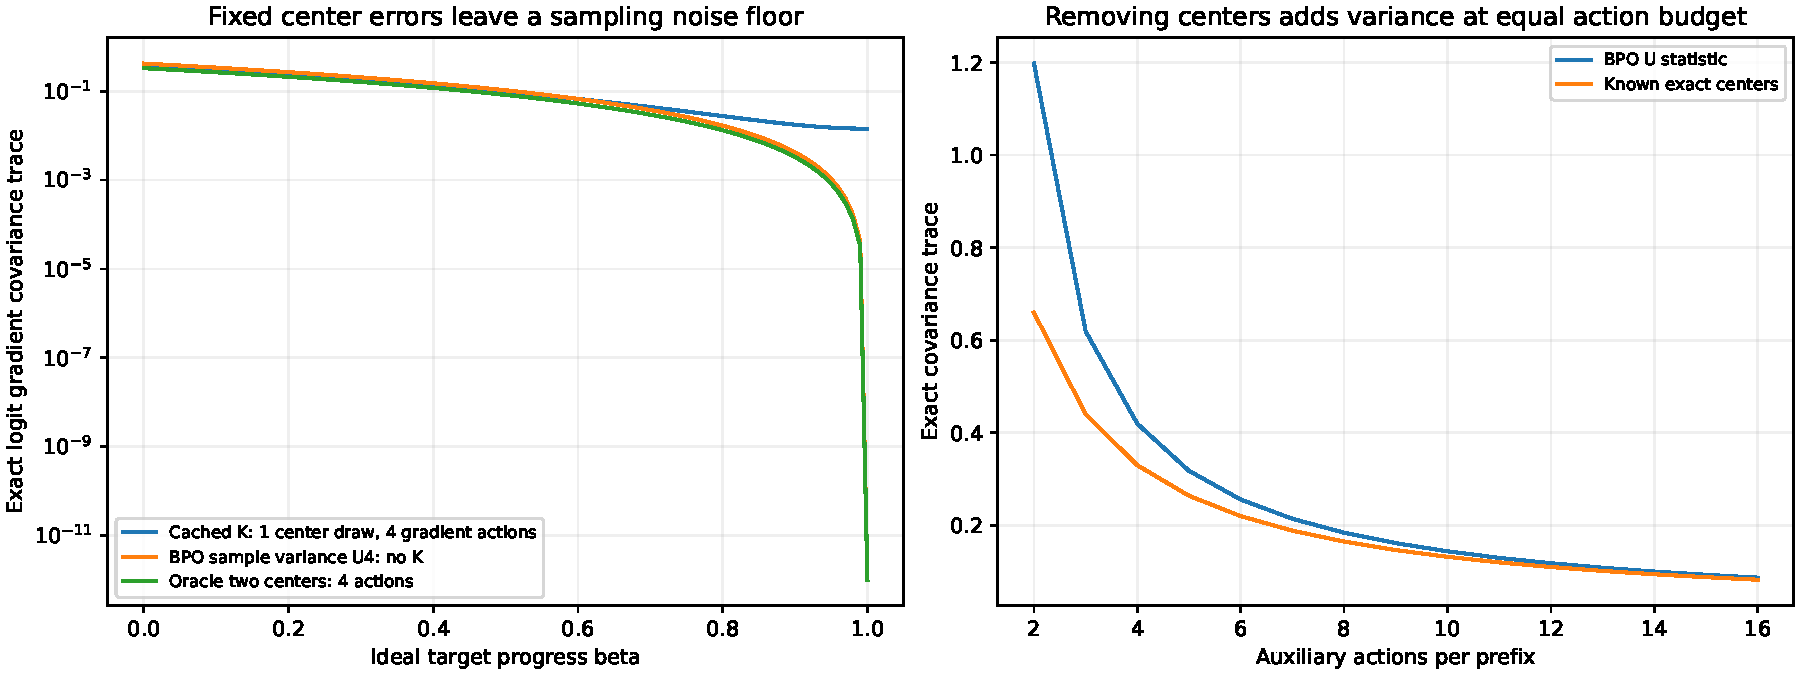
\includegraphics[width=\textwidth]{../../results/power-center-extensions/center-noise-and-sample-variance.pdf}
 \caption{理想 logits 拟合路径上，固定教师中心估计产生末期采样噪声底；BPO sample-variance 梯度的方差随残差平方下降。右图按相同辅助 action 数比较，取消两中心计算有额外方差代价。}
\end{figure}
\begin{figure}[htbp]
 \centering
 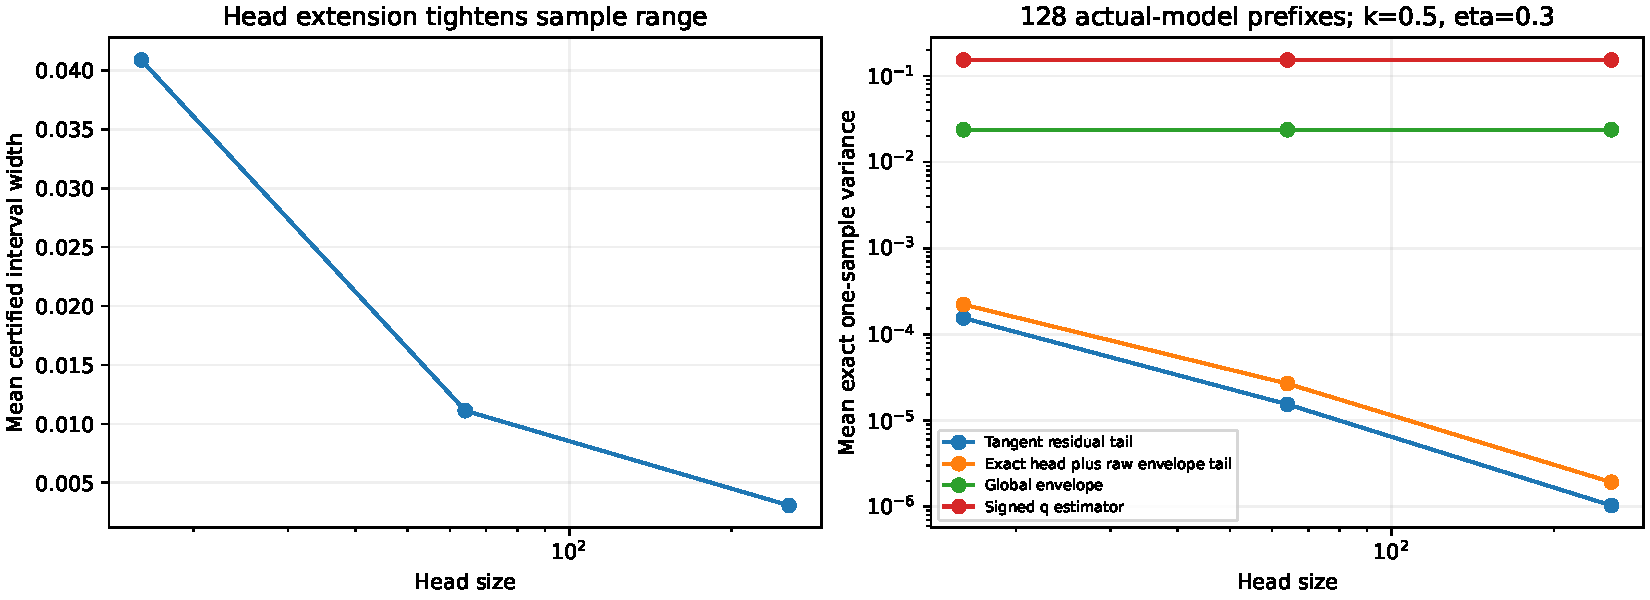
\includegraphics[width=\textwidth]{../../results/power-center-extensions/cached-head-tail-estimation.pdf}
 \caption{原模型缓存 128 个固定前缀上的 tail 区间与无偏估计器条件矩。扩大 head 收紧统一范围与置信保证；实际方差按数据读出，不声称所有输入上都优于其他估计器。}
\end{figure}

% END SOURCE: sections/proximal_action_estimators.tex


\section{高维动力学、投影与其他拟合目标}
\label{sec:power-projection}

% BEGIN SOURCE: book/sections/proximal_probability_paths.tex
\subsection{概率坐标、log-odds 与高维方向}

词表维数为 $d$ 时，每个前缀的 token 分布位于 $\Delta^{d-1}$。算术 target $m_{1,\eta}=(1-\eta)q+\eta T$ 在概率坐标中是直线。几何 target $m_{0,\eta}\propto q^{1-\eta}T^\eta$ 的 log-odds 则满足
\begin{equation}
 \log\frac{m_{0,\eta,a}}{m_{0,\eta,b}}
 =(1-\eta)\log\frac{q_a}{q_b}+\eta\log\frac{T_a}{T_b}.
\end{equation}
归一化常数在坐标差中消失；因此几何 target 在 log-odds 中是直线。这对应信息几何中的 mixture 路径和 exponential 路径\footnote{Shun-ichi Amari. Information Geometry and Its Applications: Convex Function and Dually Flat Manifold. ETVC 2008, LNCS 5416, 2009, pp. 75--102. \url{https://bsi-ni.brain.riken.jp/database/file/293/299.pdf}.}。当 teacher 极小概率接近零时，几何 target 的对应概率也可接近零，即使 $\eta$ 固定得很小；算术 target 则保留 $(1-\eta)q_a$ 的概率下界。

对 $\eta$ 在零处求导，两个方向分别为
\begin{equation}
 \left.\partial_\eta m_{1,\eta}\right|_{\eta=0}=T-q,\qquad
 \left.\partial_\eta m_{0,\eta,a}\right|_{\eta=0}
 =q_a[\log(T_a/q_a)-\E_q\log(T/q)].
\end{equation}
第一式是概率插值的直接微分。第二式使用未归一化几何密度的导数 $q_a\log(T_a/q_a)$，再减去配分函数导数对应的条件均值。高维下两方向一般不共线；统一缩放步长不能纠正方向差异。只有全部 teacher/anchor 比率一致接近一时，$\log\rho=\rho-1+O((\rho-1)^2)$ 才使两方向一阶接近。

% END SOURCE: sections/proximal_probability_paths.tex


% BEGIN SOURCE: book/sections/proximal_generalization.tex
\subsection{精确幂均值步降低所有凸生成散度}

令 $s_a=q_a/T_a$。幂均值 target 可写为 $m_a=T_aG(s_a)/Z$，其中
\begin{equation}
 G(s)=[(1-\eta)s^\kappa+\eta]^{1/\kappa},\quad
 G_0(s)=s^{1-\eta},\quad Z=\E_TG(s).
\end{equation}
$G$ 严格递增，$G(s)/s$ 严格递减。对 $\kappa>0$，第二条由
\begin{equation}
 \frac{d}{d\log s}\log\frac{G(s)}s
 =-\frac{\eta s^{-\kappa}}{1-\eta+\eta s^{-\kappa}}<0
\end{equation}
得到；几何端点导数为 $-\eta$。又有 $Z=\sum_aq_a[G(s_a)/s_a]$，故存在 $s_\star\in[\min s,\max s]$ 使 $G(s_\star)/s_\star=Z$。若 $s_a<s_\star$，则 $s_a\le G(s_a)/Z\le s_\star$；若 $s_a>s_\star$，则 $s_\star\le G(s_a)/Z\le s_a$。

\begin{theorem}[单教师的凸生成散度单调性]
\label{thm:proximal-all-f-divergences}
对任意凸函数 $\varphi:(0,\infty)\to\R$、$\varphi(1)=0$，定义 $D_\varphi(q\Vert T)=\sum_aT_a\varphi(q_a/T_a)$。精确 target 满足 $D_\varphi(m\Vert T)\le D_\varphi(q\Vert T)$。因此 $\KL(m\Vert T)$、$\KL(T\Vert m)$、Hellinger 散度、TV 和 $\chi^2(m\Vert T)$ 同时不增加。
\end{theorem}

\begin{proof}
取 $c\in\partial\varphi(s_\star)$。凸函数 $\varphi(s)-cs$ 在 $s_\star$ 取得最小值，且在其两侧分别单调不增、单调不减。每个 $s_a'=m_a/T_a=G(s_a)/Z$ 都位于 $s_a$ 与 $s_\star$ 之间，因此 $\varphi(s_a')-cs_a'\le\varphi(s_a)-cs_a$。乘以 $T_a$ 并求和，由 $\sum_aT_as_a'=\sum_aT_as_a=1$，线性项抵消，得结论。\hfill$\square$
\end{proof}

这个结论比各自 $D_\kappa$ 的单调性更强，但只直接覆盖精确 target。它并不声称有限 inner 只要降低任何一个拟合损失，就自动同时改善所有散度。
\subsection{保持 teacher 的可逆 Markov 核}

还可构造一个依赖 $q,T$ 的转移核 $\mathsf{P}$，满足 $T \mathsf{P}=T$、$q\mathsf{P}=m$。令 $\delta_a=m_a-q_a$，$L=\{a:\delta_a>0\}$、$H=\{b:\delta_b<0\}$，以及 $D=\sum_{a\in L}\delta_a=\sum_{b\in H}(-\delta_b)$。$D=0$ 时取 $\mathsf{P}=I$。否则，对 $a\in L,b\in H$ 定义
\begin{equation}
 w_{ab}=w_{ba}=\frac{\delta_a(-\delta_b)}{D(s_b-s_a)},\qquad
 \mathsf{P}_{ab}=w_{ab}/T_a,\quad \mathsf{P}_{ba}=w_{ab}/T_b,
\end{equation}
其余非对角项为零，$\mathsf{P}_{aa}=1-\sum_{b\ne a}\mathsf{P}_{ab}$。由共同交点性质，$a\in L$ 时 $\delta_a/T_a\le s_\star-s_a$，$b\in H$ 时 $(-\delta_b)/T_b\le s_b-s_\star$。所以
\begin{equation}
 \sum_{b\in H}w_{ab}\le\frac{\delta_a}{s_\star-s_a}\le T_a,\qquad
 \sum_{a\in L}w_{ab}\le\frac{-\delta_b}{s_b-s_\star}\le T_b.
\end{equation}
对角项非负，行和为一；$T_a\mathsf{P}_{ab}=T_b\mathsf{P}_{ba}$ 保证详细平衡与 $T \mathsf{P}=T$。对 $a\in L$，$(q\mathsf{P})_a-q_a=\sum_b w_{ab}(s_b-s_a)=\delta_a$；对 $b\in H$ 同样得到其损失质量，故 $q\mathsf{P}=m$。

由 $m_j/T_j=\sum_i(T_i\mathsf{P}_{ij}/T_j)s_i$ 与 Jensen 不等式，也能重新证明上一条定理。这个核是精确更新的数学表示，不要求实际构造一个词表大小平方的矩阵。它给出共同 teacher 下的保序质量转移解释，避免仅凭某个特定 KL 方向描述更新。
\subsection{目标半径随插值强度单调}

\begin{theorem}[固定锚点的目标半径单调性]
\label{thm:power-target-radius}
固定正支持 $q,T$ 与 $\kappa\in[0,1]$，对任意凸生成函数 $\varphi$，$D_\varphi(m_{\kappa,\eta}\Vert q)$ 随 $\eta\in[0,1]$ 非减少。若 $q\ne T$ 且 $\varphi$ 严格凸，则在 $0<\eta<1$ 上严格增加。Hellinger 距离及 Fisher--Rao 距离因而允许在可达范围内唯一校准 $\eta$。
\end{theorem}

\begin{proof}
对 $0<\eta_1<\eta_2<1$，记 $u_{i,a}=m_{\eta_i,a}/q_a$。$u_1$ 随 $\rho=T/q$ 严格递增，且
\begin{equation}
 \frac{m_{\eta_2,a}}{m_{\eta_1,a}}
 =\frac{Z_{\eta_1}}{Z_{\eta_2}}
 \left(\frac{1-\eta_2+\eta_2\rho_a^\kappa}
 {1-\eta_1+\eta_1\rho_a^\kappa}\right)^{1/\kappa}
\end{equation}
也随 $\rho_a$ 严格递增，因为对 $x=\rho_a^\kappa$，括号内比率的导数为 $(\eta_2-\eta_1)/(1-\eta_1+\eta_1x)^2>0$。几何端点对应 $Z_{\eta_1}\rho_a^{\eta_2-\eta_1}/Z_{\eta_2}$。其在 $m_{\eta_1}$ 下的期望为一，因此在极小和极大概率比之间有唯一的连续交点 $\rho_\star$，使 $m_{\eta_2}/m_{\eta_1}=1$。令 $u_\star=u_1(\rho_\star)$。低于交点时 $u_2\le u_1\le u_\star$，高于交点时 $u_2\ge u_1\ge u_\star$；这是向远离共同交点的方向移动。

取 $c\in\partial\varphi(u_\star)$，凸函数 $\varphi(u)-cu$ 在 $u_\star$ 两侧分别非增加、非减少。逐 action 的向外移动给出 $\varphi(u_2)-cu_2\ge\varphi(u_1)-cu_1$。乘以 $q$ 求和，线性项因 $\E_qu_i=1$ 抵消，得到
\begin{equation}
 D_\varphi(m_{\eta_2}\Vert q)\ge D_\varphi(m_{\eta_1}\Vert q).
\end{equation}
$\eta_1=0$ 时由散度非负性成立；端点一由连续性得到。若 $q\ne T$，两组 target 不同，至少一个正质量 action 严格向外移动；严格凸性使上述期望不等式严格成立。对 $\varphi(u)=(\sqrt u-1)^2$，有严格的 Hellinger 单调性。Fisher--Rao 距离是 $H^2$ 的严格递增连续函数，故具有相同结论。
\end{proof}

对不同前缀的固定加权平均，非严格单调性仍成立；面板上有正权重的 $q\ne T$ 前缀时，Hellinger 半径严格递增。相同 $\eta$ 在不同 $\kappa$ 下通常不意味着相同 target 位移。校准面板与实际比较面板不同时，半径仍需在比较面板上独立读出。
\subsection{有限 inner 的 reverse KL 与 Rényi 证书}

令 $\epsilon=\KL(p\Vert m)$、$\ell_T(a)=\log(m_a/T_a)$，$H=\max \ell_T-\min \ell_T$。恒等式为
\begin{equation}
 \KL(p\Vert T)=\epsilon+\KL(m\Vert T)+\sum_a(p_a-m_a)\ell_T(a).
\end{equation}
减去 $\ell_T$ 的区间中点后使用 Hölder 和 Pinsker 不等式，得到
\begin{equation}
 \KL(p\Vert T)\le\KL(m\Vert T)+\epsilon+H\sqrt{\epsilon/2}.
 \label{eq:proximal-range-certificate}
\end{equation}
若右侧不超过 $\KL(q\Vert T)$，则原始 teacher reverse KL 下降。这里 $H$ 可被极小概率的尾部主导，故还需要一个按概率加权的证书。

对任意 $u>0$，令 $r_u(a)=m_a^{1+u}T_a^{-u}/C_u$，$C_u=\sum_am_a^{1+u}T_a^{-u}$。由
\begin{equation}
 \KL(p\Vert r_u)=\epsilon-u\E_p\ell_T+\log C_u\ge0,
\end{equation}
得到
\begin{equation}
 \boxed{\KL(p\Vert T)\le
 \inf_{u>0}\left[(1+1/u)\KL(p\Vert m)+D_{1+u}^{\mathrm R}(m\Vert T)\right]},\quad
 D_{1+u}^{\mathrm R}(m\Vert T)=\frac1u\log C_u.
 \label{eq:proximal-renyi-certificate}
\end{equation}
有限个正 $u$ 上取最小值仍是有效上界。$u\to0$ 时，$D_{1+u}^{\mathrm R}(m\Vert T)=\KL(m\Vert T)+\tfrac u2\Var_m\ell_T+O(u^2)$。对固定分布、小拟合误差的局部展开，最优平衡项约为 $\sqrt{2\epsilon\Var_m\ell_T}$，解释了概率加权证书为何可能比区间界更紧；有限 $u$ 的精确式才是保证。相同 $u$ 下先逐 prefix 应用再固定测度求平均，也能得到整体条件目标的上界。

% END SOURCE: sections/proximal_generalization.tex


% BEGIN SOURCE: book/sections/proximal_dynamics.tex
\subsection{精确外层与有限 inner 的散度进展}

\begin{theorem}[teacher 散度的进展恒等式]
\label{thm:proximal-teacher-progress}
记 $c_\kappa=Z^\kappa$，端点 $\kappa=0,1$ 取 $c_\kappa=1$。对任意候选 $p$，有
\begin{equation}
 \eta\left[D_\kappa(T\Vert q)-D_\kappa(T\Vert p)\right]
 =(1-\eta)D_\kappa(q\Vert p)
 +c_\kappa\left[D_\kappa(m\Vert q)-D_\kappa(m\Vert p)\right].
 \label{eq:proximal-progress-identity}
\end{equation}
若 $D_\kappa(m\Vert p)\le D_\kappa(m\Vert q)$，则 teacher 散度不会增加。精确更新 $p=m$ 且 $q\ne T$ 时严格下降。
\end{theorem}

\begin{proof}
$F(q)=\eta D_\kappa(T\Vert q)$，而 $F(p)=(1-\eta)D_\kappa(q\Vert p)+\eta D_\kappa(T\Vert p)$。由定理~\ref{thm:proximal-barycenter-gap}，$F(q)-F(p)=c_\kappa[D_\kappa(m\Vert q)-D_\kappa(m\Vert p)]$。将 $F(q),F(p)$ 的定义代入并移项，即得恒等式。若目标散度改善，右侧两项非负；若 $p=m$、$q\ne T$，$m\ne q$，则至少第一项严格为正。最后，$m=q$ 会要求 $T_a^\kappa$ 与 $q_a^\kappa$ 成同一比例，概率归一化强制 $T=q$；两个端点同样成立。\hfill$\square$
\end{proof}

这给出了一个纯数学的 finite-inner 条件：降低本轮的 $D_\kappa(m\Vert p)$ 就能提高同一 $D_\kappa$ 下的 teacher 接近度。这里 teacher 散度的方向随 $\kappa$ 改变；一般 $\kappa$ 的保证不能直接替换成每步 $\KL(p\Vert T)$ 都下降。用其他拟合损失获得同一 target，只能在精确求解时自动继承本结论。
\subsection{escort 坐标中的线性轨迹与全局收敛}

对 $\kappa>0$ 定义 escort 分布和幂和
\begin{equation}
 E_\kappa(q)_a=\frac{q_a^\kappa}{S_\kappa(q)},\qquad
 S_\kappa(q)=\sum_aq_a^\kappa.
\end{equation}
$E_\kappa$ 是单纯形上的双射，逆映射为 $q_a\propto E_\kappa(q)_a^{1/\kappa}$。由 $m_a^\kappa=S_a/Z^\kappa$，共同的归一化因子在 escort 中消失，故
\begin{equation}
 E_\kappa(m)=(1-a^{\mathrm{esc}})E_\kappa(q)+a^{\mathrm{esc}}E_\kappa(T),\qquad
 a^{\mathrm{esc}}=\frac{\eta S_\kappa(T)}{(1-\eta)S_\kappa(q)+\eta S_\kappa(T)}.
 \label{eq:proximal-escort-step}
\end{equation}
这是精确式，不是局部近似。$\kappa=1$ 时 $S_1=1$，恢复 $a^{\mathrm{esc}}=\eta$；$0<\kappa<1$ 时，$S_\kappa(q)=\exp((1-\kappa)H_\kappa(q))$，其中 $H_\kappa$ 是 Rényi 熵。因此固定的概率幂插值强度在 escort 坐标中表现为随分布熵改变的有效步幅。

\begin{figure}[htbp]
 \centering
 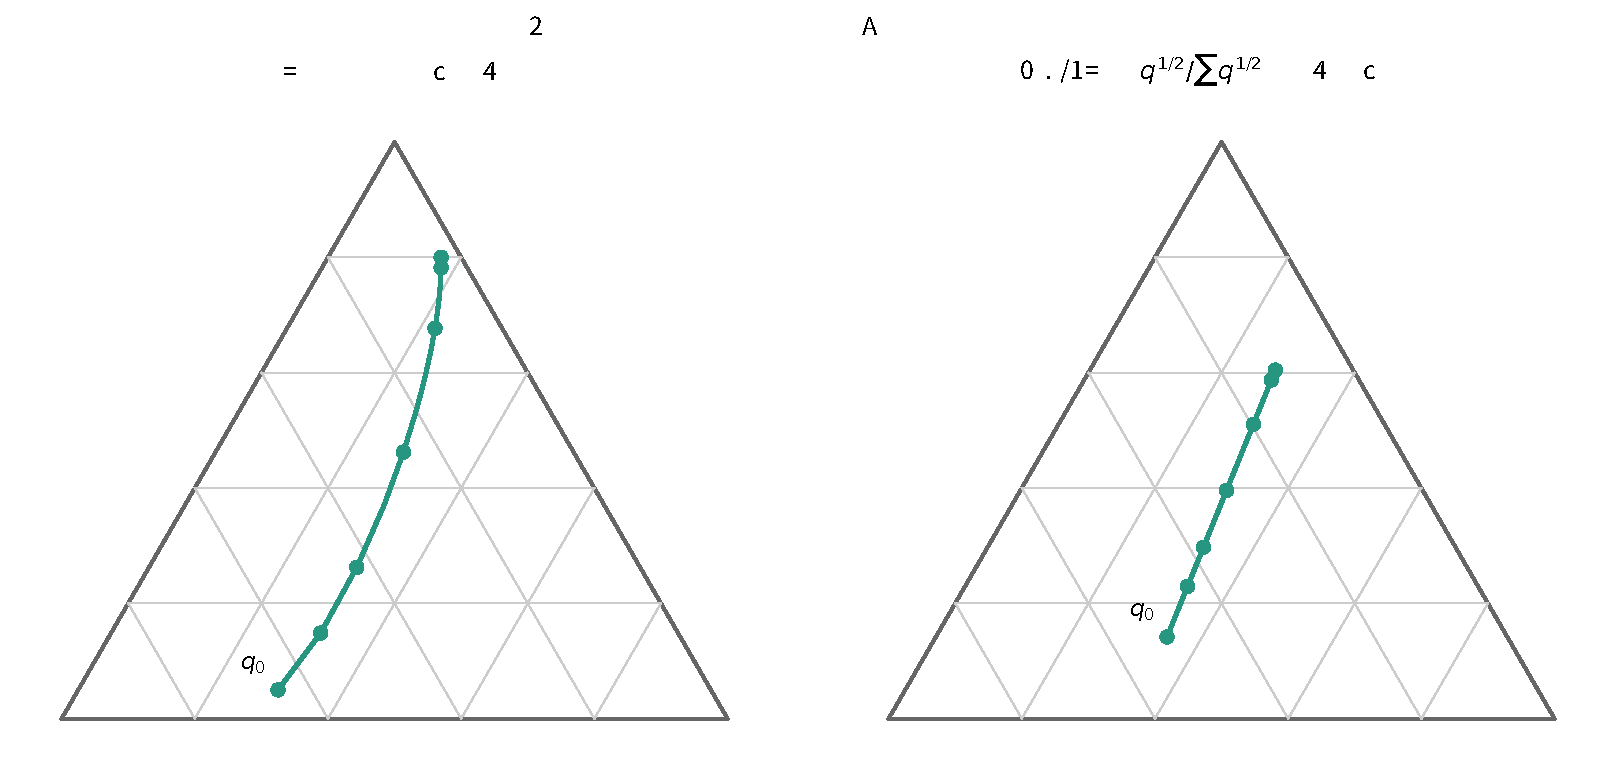
\includegraphics[width=\textwidth]{../../results/proximal-family-geometry/escort.pdf}
 \caption{同一平方根外层轨迹在概率坐标中弯曲，在 escort 坐标中是直线。圆点和数字表示迭代时点。高维分量在固定教师下共享一个进度系数。}
\end{figure}

若 $q_{n+1}=m_{\kappa,\eta}(q_n,T)$，记 $e_n=E_\kappa(q_n)$，则
\begin{equation}
 e_n-e_T=b_n(e_0-e_T),\qquad
 b_n=\prod_{j=0}^{n-1}(1-a_j^{\mathrm{esc}}).
 \label{eq:proximal-escort-orbit}
\end{equation}
这将固定教师下的 $d-1$ 维精确外层轨迹归结为一个标量 $b_n$。对连续自然梯度流，$dq_a/dt=q_a(\rho_a^\kappa-a_\kappa)/\kappa$，所以
\begin{align}
 \frac{d}{dt}q_a^\kappa&=T_a^\kappa-a_\kappa q_a^\kappa,\\
 \frac{d}{dt}S_\kappa(q)&=S_\kappa(T)-a_\kappa S_\kappa(q),\\
 \frac{d}{dt}E_\kappa(q)&=\frac{S_\kappa(T)}{S_\kappa(q)}[E_\kappa(T)-E_\kappa(q)].
\end{align}
改用时间 $\sigma$，$d\sigma/dt=S_\kappa(T)/S_\kappa(q)>0$，就有 $e(\sigma)=e_T+e^{-\sigma}(e_0-e_T)$。离散步式~\eqref{eq:proximal-escort-step} 也位于同一条流轨迹上，对应时间增量 $-\log(1-a^{\mathrm{esc}})$。精确幂均值步因此是这个自然梯度流轨迹的一种时间重参数化，而不只是具有相同起始切线。

\begin{theorem}[teacher 定向的 escort 收缩与误差累积]
\label{thm:proximal-escort-contraction}
令 $d$ 为词表大小，$0<\kappa\le1$，定义度量 $d_\kappa(q,T)=\|E_\kappa(q)-E_\kappa(T)\|_1$。对固定 teacher 的精确更新有
\begin{equation}
 d_\kappa(q_{n+1},T)=(1-a_n^{\mathrm{esc}})d_\kappa(q_n,T)\le c\,d_\kappa(q_n,T),\quad
 c=\frac{(1-\eta)d^{1-\kappa}}{(1-\eta)d^{1-\kappa}+\eta S_\kappa(T)}<1.
\end{equation}
故 $q_n\to T$。若近似更新满足 $d_\kappa(q_{n+1},m(q_n,T))\le\epsilon_n$，则
\begin{equation}
 d_\kappa(q_n,T)\le c^nd_\kappa(q_0,T)+\sum_{j=0}^{n-1}c^{n-1-j}\epsilon_j,
 \qquad
 \limsup_nd_\kappa(q_n,T)\le\frac{\epsilon_\infty}{1-c}
\end{equation}
其中最后一式要求 $\limsup_n\epsilon_n\le\epsilon_\infty$。
\end{theorem}

\begin{proof}
式~\eqref{eq:proximal-escort-step} 给出距离的精确比例。Jensen 不等式给出 $S_\kappa(q)\le d^{1-\kappa}$，因此 $1-a_n^{\mathrm{esc}}\le c$。反复应用得到精确更新的 $c^n$ 界；escort 逆映射连续，故 $q_n\to T$。近似更新时，三角不等式给出 $d_\kappa(q_{n+1},T)\le\epsilon_n+c\,d_\kappa(q_n,T)$，展开得到有限步式。对任意 $\delta>0$，取 $N$ 使 $j\ge N$ 时 $\epsilon_j\le\epsilon_\infty+\delta$。有限个早期项乘以 $c^{n-1-j}$ 后趋于零，后期项的和不超过 $(\epsilon_\infty+\delta)\sum_{i\ge0}c^i$。令 $\delta\to0$ 得极限上界。\hfill$\square$
\end{proof}

这是对固定 teacher 的定向收缩，不声称两个任意 anchor 经同一算子后具有同一个收缩系数；它也不直接等于原概率空间的 TV 收缩。$\kappa\to0$ 时，escort 本身趋于均匀分布，必须重标度才保留信息：
\begin{equation}
 \frac d\kappa\left[E_\kappa(q)_a-\frac1d\right]
 \longrightarrow\log q_a-\frac1d\sum_b\log q_b.
\end{equation}
几何端点就在这些中心化 log 坐标中满足精确比例 $1-\eta$。在任何固定完整支持的 teacher 附近，所有 $\kappa$ 都有 $m(T+\delta,T)=T+(1-\eta)\delta+O(\|\delta\|^2)$，因为 $a_n^{\mathrm{esc}}\to\eta$。它们共享局部收敛率，远处的度量和有效时间则不同。

\begin{figure}[htbp]
 \centering
 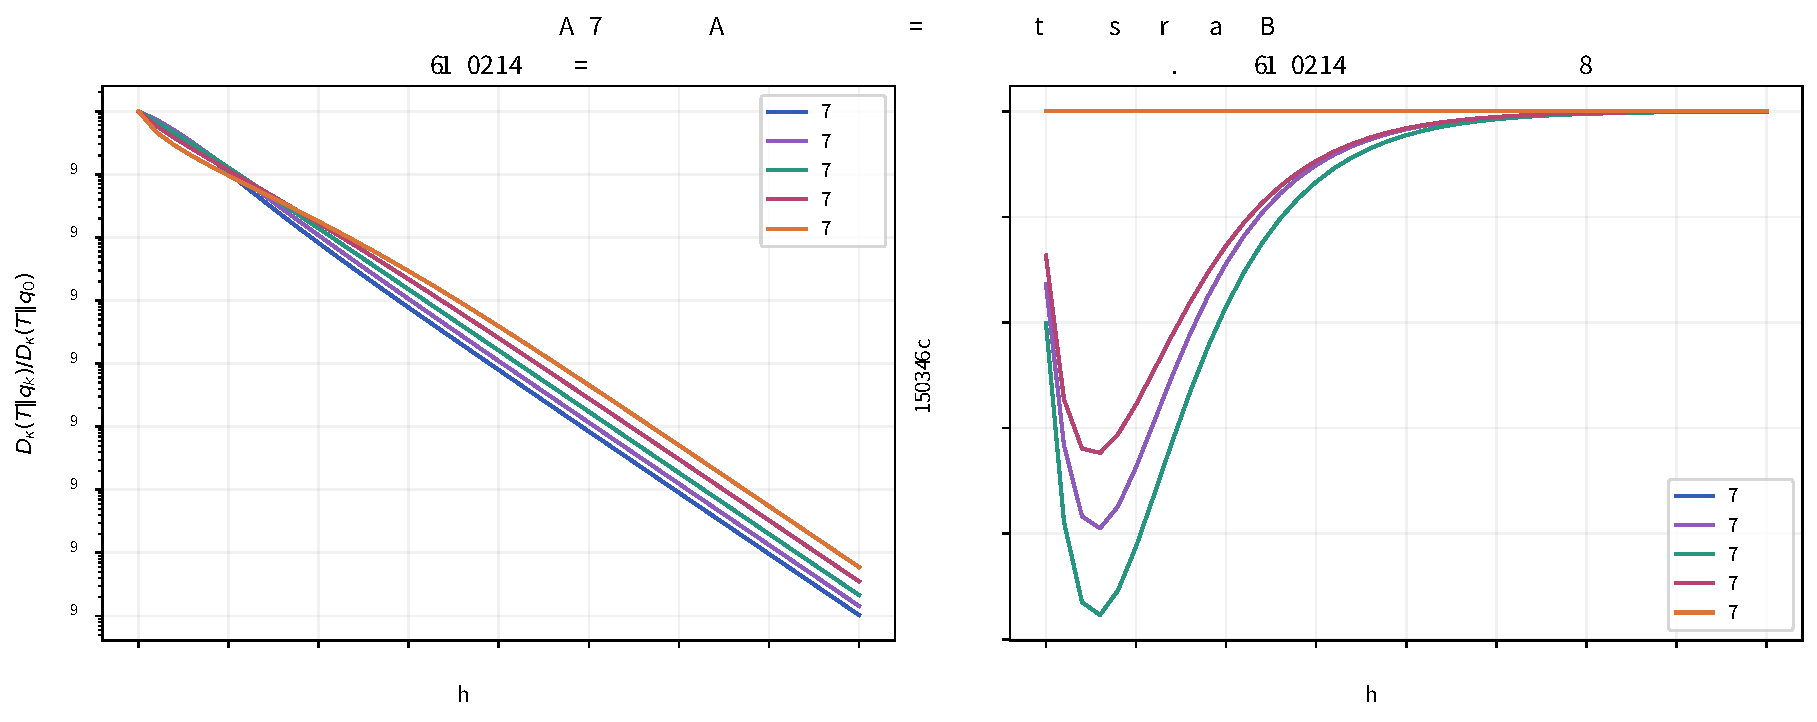
\includegraphics[width=\textwidth]{../../results/proximal-family-geometry/convergence.pdf}
 \caption{精确外层的 teacher 散度单调下降，有效 escort 步幅趋于共同的 $\eta$。每条曲线使用各自的 $D_\kappa$ 并按初值归一化，图中的高低不能直接作为同一任务的训练性能排名。}
\end{figure}
\subsection{共享参数子流形上的自然梯度投影}

独立 token 分布的速度界还可延伸到共享参数的自然梯度流，但需要明确度量。取有限个 prefix、固定权重 $d_s>0$、$\sum_sd_s=1$，将外层分布写成 $q_\theta(a\mid s)>0$。定义
\begin{equation}
 L_\kappa(\theta)=\sum_sd_sD_\kappa(T_s\Vert q_{\theta,s}),\qquad
 \langle v,w\rangle_W=\sum_{s,a}\frac{d_s}{q_{\theta,s,a}}v_{s,a}w_{s,a}.
\end{equation}
记 $J=\partial q_\theta/\partial\theta$，$W=\operatorname{diag}(d_s/q_{\theta,s,a})$，则参数 Fisher 矩阵为 $\mathcal I=J^\top WJ$。令 $v$ 为每个 prefix 上的无约束负自然梯度，$v_{s,a}=q_{\theta,s,a}(\rho_{s,a}^\kappa-\E_{q_{\theta,s}}\rho_s^\kappa)/\kappa$。因为每个 prefix 的 $J$ 列向量分量和为零，$\nabla_\theta L=-J^\top Wv$。

参数自然梯度流采用 Moore--Penrose 广义逆 $\mathcal I^+$ 时，有
\begin{equation}
 \dot\theta=-\mathcal I^+\nabla_\theta L,\qquad
 \dot q_\theta=J\mathcal I^+J^\top Wv=Pv.
\end{equation}
$P$ 是到 $\operatorname{range}(J)$ 的 $W$ 正交投影：令 $B=W^{1/2}J$，则 $W^{1/2}PW^{-1/2}=B(B^\top B)^+B^\top$，后者是普通欧氏正交投影。因此
\begin{equation}
 \|\dot q_\theta\|_W^2\le\|v\|_W^2,\qquad
 \frac{dL}{dt}=-\langle v,Pv\rangle_W=-\|Pv\|_W^2\le0.
\end{equation}
平方根形状满足 $\|v\|_W^2=\sum_sd_s\,4(1-a_s^2)\le4$，所以共享参数的精确自然梯度流也满足 $\|\dot q_\theta\|_W\le2$。更一般地，$0<\kappa\le1/2$ 时平方速度不超过 $1/\kappa^2$。

这个结论控制的是分布流在固定 prefix Fisher 度量下的速度。它不控制参数的欧氏范数，也不自动适用于普通梯度流。共享参数还可能使 $Pv=0$ 而 $q_\theta\ne T$，因此单调性和速度界并不保证无投影误差的 teacher 收敛。离散幂均值 target 的精确 escort 轨迹也不会因这个局部投影结论自动延续到共享参数模型。

% END SOURCE: sections/proximal_dynamics.tex


% BEGIN SOURCE: book/sections/proximal_self_bounding.tex
\subsection{target 形状与拟合形状是两个参数}

前文 $\kappa$ 用于构造 $m_{\kappa,\eta}$，本小节明确写为 $\kappa_{\mathrm{target}}$。拟合一个已经冻结的 $m$ 时，可以另外选择 $\kappa_{\mathrm{fit}}$，最小化 $D_{\kappa_{\mathrm{fit}}}(m\Vert p)$。前文的重心进展恒等式直接对应两者相等的情形；两者不相等时仍共享最优点 $p=m$，但有限 inner 应使用 reverse KL/Rényi 证书或另行证明共同评价目标的进展。

因此，几何 target 可以搭配 Hellinger 拟合，算术 target 也可以搭配 Hellinger 拟合。下面的最优常数结论作用于拟合形状，不能直接宣称平方根 target 对任何任务都最优。

\subsection{当前学生采样的误差相关梯度矩界}

固定 prefix 和 target $m$，本小节记 $k=\kappa_{\mathrm{fit}}$。从当前学生 $a\sim p$ 采样动作，令 $\chi=m/p$、$a_k=\E_p\chi^k$、$\psi_p=\nabla_\theta\log p$。解析微分 $D_k(m\Vert p)$，并利用 $\E_p\psi_p=0$，得到无偏估计量
\begin{equation}
 g_k(a)=\frac{a_k-\chi_a^k}{k}\psi_p(a),\qquad
 \E_pg_k=\nabla_\theta D_k(m\Vert p).
\end{equation}
它在 $p=m$ 时逐 action 为零。前缀保持固定、动作从当前学生重采样，与每步重新生成完整 response 是两种不同的测度操作。

\begin{theorem}[误差相关二阶矩的锐常数]
\label{thm:proximal-sharp-self-bound}
若 $\|\psi_p(a)\|\le S$、$0<k\le1/2$，则
\begin{equation}
 \Var_p(g_k)\le\E_p\|g_k\|^2
 \le\frac{S^2}{k}D_k(m\Vert p).
\end{equation}
系数 $1/k$ 是对所有完整支持概率分布统一成立的锐常数。$k=0$ 或 $k>1/2$ 没有有限的统一误差相关常数。按此标准，$k=1/2$ 是该规范化散度族中的唯一最佳形状。
\end{theorem}

\begin{proof}
令 $a(u)=\E_p\chi^u$，则 $a(1)=1$，$a$ 对 $u$ 凸，且 $a(k)\le1$。由于 $2k\in[k,1]$，凸性给出
\begin{equation}
 a(2k)\le\frac{1-2k}{1-k}a(k)+\frac{k}{1-k}.
\end{equation}
所以
\begin{align}
 \Var_p(\chi^k)&=a(2k)-a(k)^2\\
 &\le\frac{(1-a(k))[k+(1-k)a(k)]}{1-k}\\
 &\le\frac{1-a(k)}{1-k}.
\end{align}
再由 $D_k(m\Vert p)=(1-a(k))/[k(1-k)]$，得到 $\E_p[(a_k-\chi^k)^2/k^2]\le D_k/k$，乘以 score 范数界即可。

为证明锐性，取 $p=(v,1-v)$、$m=(v^2,1-v^2)$，$v\to0$。比率为 $\chi=(v,1+v)$，因此 $a(k)=1-(1-k)v+o(v)$、$a(2k)=1-(1-2k)v+o(v)$，有 $\Var_p\chi^k=v+o(v)$、$D_k=v/k+o(v)$。系数二阶矩与损失之比趋于 $1/k$。categorical logits 的 rare-action score 范数平方趋于 2，其概率为 $v$，common-action score 范数平方为 $O(v^2)$，故实际梯度二阶矩也达到这个相对常数；均值平方为 $O(v^2)$，方差具有同一极限。

$1/2<k<1$ 时，取 $p=(v,1-v)$、$m=(1/2,1/2)$，系数方差按 $v^{1-2k}$ 发散，但 $D_k\le1/[k(1-k)]$。$k=1$ 时系数方差按 $1/v$ 发散，损失只按 $\log(1/v)$ 增长。$k=0$ 的 centred log-ratio 系数二阶矩可按 $\log^2(1/m_a)$ 增长，而 reverse KL 只按 $\log(1/m_a)$ 增长。取非对称、固定正质量的学生即可使梯度方差与损失的比也发散。\hfill$\square$
\end{proof}

在平方根点，这个关系更精确：$a=\sum\sqrt{pm}$，$D_{1/2}=4(1-a)$，系数二阶矩为 $4(1-a^2)=D_{1/2}(1+a)$。它既有统一绝对上界 4，也随拟合误差消失。若使用损失 $L=D_{1/2}/\eta$，对应的缩放梯度满足 $\E\|g/\eta\|^2\le(2S^2/\eta)L$。模型投影误差不为零时，这个结论不强制噪声消失。

\subsection{精确 BPO 已有残差驱动的噪声控制}

对任意 target $m$ 与冻结 anchor $q$，定义 $R=C_q\log(p/m)$ 和 $L_{\mathrm{BPO}}=\E_qR^2/(2\eta)$。解析梯度中 centre 的导数乘以 $\E_qR=0$ 后消失，因此 $g=R\psi_p/\eta$ 是 anchor 动作采样的无偏估计量，并满足
\begin{equation}
 \E_q\|g\|^2\le\frac{S^2}{\eta^2}\E_qR^2
 =\frac{2S^2}{\eta}L_{\mathrm{BPO}}.
\end{equation}
所以误差相关的噪声控制不只存在于 Hellinger 拟合；BPO 本来就具有这项性质。区别是 BPO 残差损失可任意大，而 Hellinger 损失不超过 4。几何 target 的初始 BPO 误差仍可能由极端 teacher log-ratio 主导；改变 target 的形状可以控制这个初始误差。生产 Top-$J$ centre 与完整词表条件均值之间的偏差，必须与这个精确结论区分。

\subsection{平方根 target 和平方根拟合的初始矩界}

若 $m=m_{1/2,\eta}(q,T)$，令 $a=\sum\sqrt{qT}$、$Z=(1-\eta)^2+\eta^2+2\eta(1-\eta)a$。在 inner 起点 $p=q$，有
\begin{equation}
 \sum_a\sqrt{q_am_a}=\frac{1-\eta+\eta a}{\sqrt Z},\qquad
 1-\left(\sum_a\sqrt{q_am_a}\right)^2=\frac{\eta^2(1-a^2)}Z.
\end{equation}
因此平方根拟合的梯度系数在除以 $\eta$ 后，二阶矩为 $4(1-a^2)/Z\le4/[(1-\eta)^2+\eta^2]\le8$。这给出同时对所有 teacher、anchor 和 $0<\eta<1$ 成立的初始上界；其 Fisher--Rao 目标位移也由相同的角度恒等式控制。这个干净的联合性质支持研究平方根组合，但不等于所有数据上的最高信噪比或最佳任务成绩。

\subsection{局部 SGD 收敛与投影误差的条件结论}

\begin{theorem}[误差相关噪声下的条件 SGD 收敛]
\label{thm:power-conditional-sgd}
固定前缀测度，设最小投影损失为 $L_\star\ge0$。假设所有随机更新线段所在区域中 $L$ 为 $L_{\mathrm{sm}}$ 光滑，满足 Polyak--\L{}ojasiewicz（PL）条件 $\|\nabla L\|^2\ge2\mu(L-L_\star)$，且当前参数固定后的估计量满足 $\E[g\mid\theta]=\nabla L$、$\E[\|g\|^2\mid\theta]\le CL$。固定
\begin{equation}
 0<\alpha_{\mathrm{opt}}\le\min\{1/\mu,2\mu/(L_{\mathrm{sm}}C)\},\qquad
 c_{\mathrm{SGD}}=1-\mu\alpha_{\mathrm{opt}}\in[0,1).
\end{equation}
则 SGD 迭代满足
\begin{equation}
 \E[L(\theta_N)-L_\star]
 \le c_{\mathrm{SGD}}^N[L(\theta_0)-L_\star]
 +\frac{L_{\mathrm{sm}}C\alpha_{\mathrm{opt}}L_\star}{2\mu}(1-c_{\mathrm{SGD}}^N).
\end{equation}
目标可实现且 $L_\star=0$ 时，残差驱动的采样噪声不产生固定步长误差底；$L_\star>0$ 时上式明确给出投影误差对应的噪声项。
\end{theorem}

\begin{proof}
令 $\theta^+=\theta-\alpha_{\mathrm{opt}}g$。光滑性、无偏性和二阶矩界给出
\begin{align}
 \E[L(\theta^+)\mid\theta]
 &\le L-\alpha_{\mathrm{opt}}\|\nabla L\|^2+
 \frac{L_{\mathrm{sm}}\alpha_{\mathrm{opt}}^2}2\E\|g\|^2\\
 &\le L-2\mu\alpha_{\mathrm{opt}}(L-L_\star)
 +\frac{L_{\mathrm{sm}}C\alpha_{\mathrm{opt}}^2}{2}L.
\end{align}
将 $L=(L-L_\star)+L_\star$ 代入，再使用 $L_{\mathrm{sm}}C\alpha_{\mathrm{opt}}^2/2\le\mu\alpha_{\mathrm{opt}}$，得到
\begin{equation}
 \E[L(\theta^+)-L_\star\mid\theta]
 \le c_{\mathrm{SGD}}(L-L_\star)+L_{\mathrm{sm}}C\alpha_{\mathrm{opt}}^2L_\star/2.
\end{equation}
对全体历史求期望，递推 $N$ 次并使用 $\sum_{j=0}^{N-1}c_{\mathrm{SGD}}^j=(1-c_{\mathrm{SGD}}^N)/(\mu\alpha_{\mathrm{opt}})$，得到结论。
\end{proof}

这些是带明确光滑性、PL、可实现性和 score 条件的 SGD 结论。共享参数模型与实际优化器需要分别核实这些假设；条件 SGD 定理不能直接作为大模型训练的保证。

% END SOURCE: sections/proximal_self_bounding.tex


% BEGIN SOURCE: book/sections/proximal_multi_teacher.tex
\subsection{同一重心恒等式的多分布扩展}

多个固定分布 $T^{(j)}$、权重 $w_j\ge0$、$\sum_jw_j=1$ 时，同一证明给出
\begin{equation}
 \argmin_p\sum_jw_jD_\kappa(T^{(j)}\Vert p)
 \propto\left[\sum_jw_j(T^{(j)})^\kappa\right]^{1/\kappa}.
\end{equation}
完整支持下，几何、平方根与算术的多教师汇合均在同一框架内；可将 anchor 作为其中一个分布。超额损失分解及最优点的 Fisher 曲率也直接延续。


% END SOURCE: sections/proximal_multi_teacher.tex


\section{序列边界与可用性质}
\label{sec:power-scope}

% BEGIN SOURCE: book/sections/proximal_sequence_scope.tex
\subsection{条件分布的改善与完整轨迹的改善}

在固定长度 $H$ 的 autoregressive 模型中，记完整序列分布为 $Q(y)=\prod_iq(y_i\mid y_{<i})$、$T(y)=\prod_it(y_i\mid y_{<i})$。KL 链式法则给出
\begin{equation}
 \KL(Q\Vert T)=\sum_{i=1}^H\E_{s_i\sim Q}\KL(q(\cdot\mid s_i)\Vert T(\cdot\mid s_i)).
 \label{eq:proximal-sequence-chain}
\end{equation}
更新每个条件分布后，访问测度也从 $Q$ 变成 $P$。因此逐个 prefix 的条件 KL 下降，不足以让这条随策略改变权重的总和下降。本书固定测度问题明确冻结权重；序列混合与逐 token 混合是不同算子。

\paragraph{一个两步、完整支持的反例。}
第一步取 $q_0=(0.99,0.01)$、$T_0=(0.01,0.99)$。第一分支的第二步取 $q_A=T_A=(1/2,1/2)$；第二分支取 $q_B=(1-10^{-6},10^{-6})$、$T_B=(10^{-30},1-10^{-30})$。在全部三个条件分布上同时执行精确幂均值步，$\eta=0.1$。每个条件 KL 都下降或保持零，但完整序列的 reverse KL 为
\begin{center}
\begin{tabular}{lrr}
\toprule
形状 & 更新前完整序列 KL & 更新后完整序列 KL\\
\midrule
$\kappa=0$ & 5.19399 & 6.07445\\
$\kappa=1/2$ & 5.19399 & 7.09792\\
$\kappa=1$ & 5.19399 & 10.44581\\
\bottomrule
\end{tabular}
\end{center}
数值由 \path{results/power-mean-20261013/generalization-checks.json} 的完整精度记录为准。变化的原因是学生更频繁进入尚未拟合好的第二分支。算术形状将该分支概率从 $0.01$ 提升到 $0.108$，其条件误差仍然很大。保持原访问权重的条件 KL 总和却从 $5.19399$ 降到 $4.38503$；两种测度给出不同结论。这个反例在固定两步时域已成立，不依赖 EOS 或长度归一化。

\begin{figure}[htbp]
 \centering
 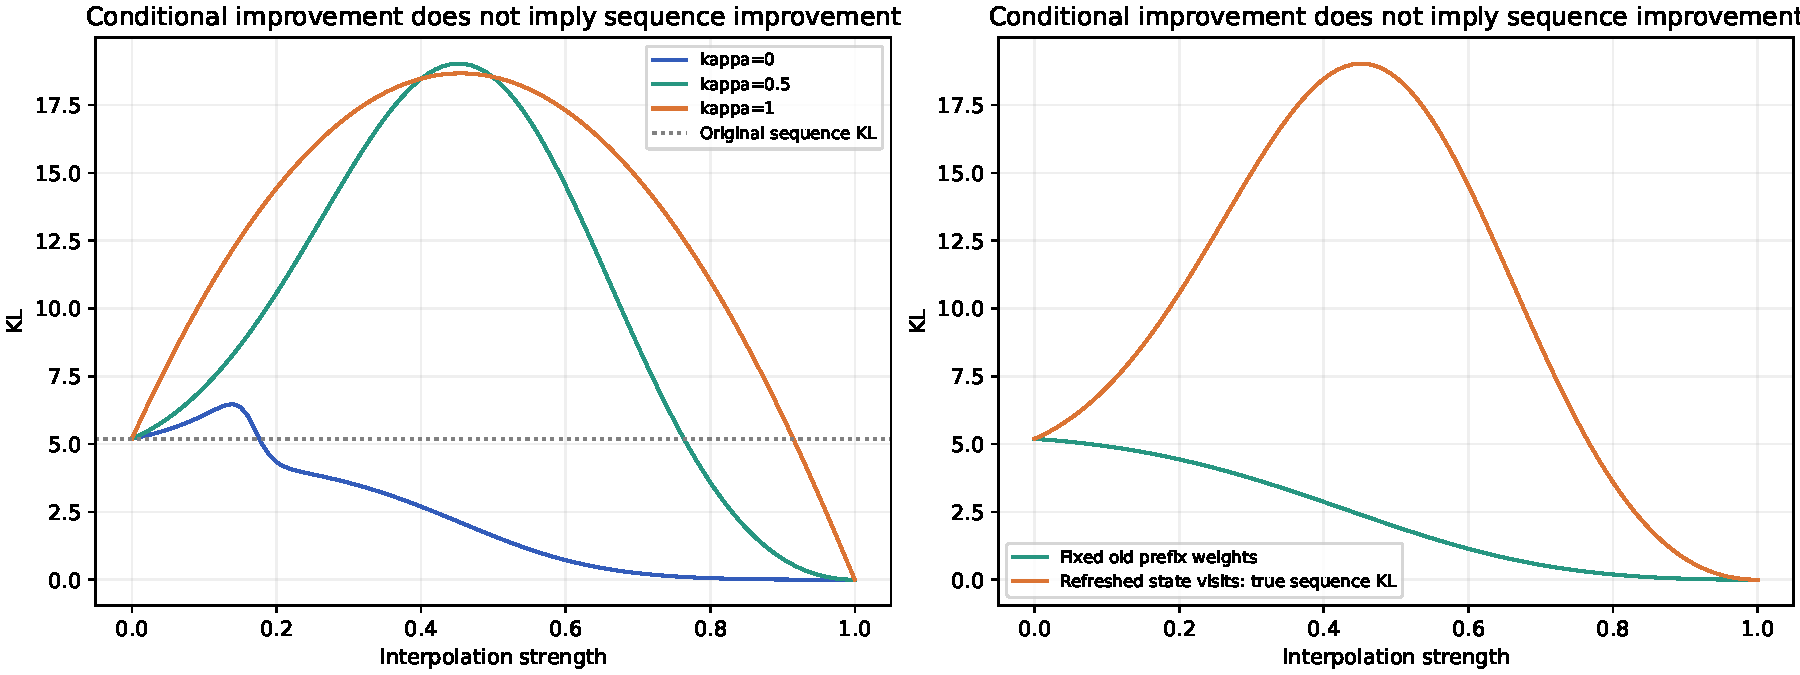
\includegraphics[width=\textwidth]{../../results/power-mean-20261013/sequence-scope-counterexample.pdf}
 \caption{精确条件更新仍可能使完整序列 KL 上升。左图比较三种形状；右图固定平方根形状，对照冻结旧 prefix 权重的条件目标与更新后访问测度下的真实序列 KL。}
\end{figure}

\subsection{序列混合的条件概率包含额外因子}

对序列层面的算术混合 $M=(1-\eta)Q+\eta T$，条件分布为
\begin{equation}
 M(a\mid s)=(1-\eta_s)q(a\mid s)+\eta_st(a\mid s),\qquad
 \eta_s=\frac{\eta T(s)}{(1-\eta)Q(s)+\eta T(s)}.
\end{equation}
它的 teacher 权重依赖已经生成的 prefix。固定 $\eta$ 的逐 token 算术混合因此一般不同于序列层面的算术混合。

对序列几何 target $M(y)\propto Q(y)^{1-\eta}T(y)^\eta$，定义后缀配分函数
\begin{equation}
 Z_\eta(s)=\sum_zQ(z\mid s)^{1-\eta}T(z\mid s)^\eta.
\end{equation}
将带前缀 $s$ 的序列质量先求和再作条件化，得到
\begin{equation}
 M(a\mid s)=q(a\mid s)^{1-\eta}T(a\mid s)^\eta
 \frac{Z_\eta(sa)}{Z_\eta(s)}.
\end{equation}
逐 token 几何 target 忽略了 action 相关的后缀配分函数；它只有在这些后缀因子与 action 无关时才恢复完整序列 target。两个端点都展示了条件化与混合一般不能交换。

\subsection{真实序列 reverse KL 的一阶方向}

记 suffix 值 $V^q(s)=\KL(Q(\cdot\mid s)\Vert T(\cdot\mid s))$。链式法则给出递推
\begin{equation}
 V^q(s)=\E_{a\sim q(\cdot\mid s)}[\log(q(a\mid s)/T(a\mid s))+V^q(sa)],
\end{equation}
终点的值为零。完整序列 KL 的 policy gradient 是
\begin{equation}
 \nabla\KL(Q\Vert T)
 =\E_Q\sum_i\psi_i\sum_{j\ge i}\log\frac{q(y_j\mid s_j)}{T(y_j\mid s_j)}.
\end{equation}
推导时，$\nabla\log Q=\sum_i\psi_i$，直接微分 KL 多出的 $\E_Q\nabla\log Q$ 为零；过去 reward 与当前 score 的乘积则因条件零均值而消失。对某个 prefix 的局部方向，未来成本不能省略；其负信号是
\begin{equation}
 f_{\mathrm{seq}}^q(s,a)=\log\frac{T(a\mid s)}{q(a\mid s)}-V^q(sa).
\end{equation}
条件中心化后，它给出真实序列 reverse KL 的自然梯度方向。即时 log-ratio 的固定测度优化只保留第一项。长度平均的未来 return、随机组标准化或其他信号变换需要另行解释其目标，不能直接继承这条精确 policy gradient。

若直接在有限序列空间构造幂均值 target，前面的凸生成散度与矩定理仍然成立。该空间虽有指数级的序列数，归一化的二阶矩界不含空间大小。若每个 token score 范数不超过 $S$，$H$ 有限，则序列 score 范数不超过 $HS$，对应的梯度二阶矩界只增加 $H^2S^2$ 因子。序列 target 的表达、采样和投影是不同问题；固定 prefix 理论与任务正确率是不同证据，须分别报告。

% END SOURCE: sections/proximal_sequence_scope.tex


% BEGIN SOURCE: book/sections/proximal_scope_summary.tex
\subsection{固定条件问题中可以直接使用的性质}

单教师的幂均值框架提供了三个相互连接的保证。正形状 $\kappa>0$ 改变极端教师概率比的尾部；固定 $(\kappa,\eta)$ 的精确更新下降一个明确的有界教师目标 $\mathcal J$；$0<\kappa\le1/2$ 的中心化监督方差又由中心 $K$ 控制。BPO 拟合的残差采样梯度随其损失下降而消失，形状变换与残差回归分别控制初始监督和拟合末期的噪声。

\begin{center}
\small
\begin{tabular}{p{46mm}p{54mm}p{45mm}}
\toprule
可用性质 & 必要条件 & 实际含义\\
\midrule
精确 target 同时改善全部凸 $f$ 散度 & 同一固定 teacher、完整正支持 & 同一评价量下可比较不同形状\\
教师覆盖与刷新后的双侧监督界 & $\kappa>0$，同一前缀精确刷新 & $q_n\ge\eta^{1/\kappa}T$，控制未来正尾部\\
精确 MD 下降与最后迭代界 & 固定 $\kappa,\eta$，每步刷新锚点 & $\mathcal J(q_N)\le\KL(T\Vert q_0)/(\eta N)$\\
教师监督方差受误差控制且可求和 & $0<\kappa\le1/2$，精确外层 & 教师接近度与监督噪声共同趋零\\
BPO 的零残差零采样梯度 & target 可实现、精确中心或无偏差分损失 & 避免固定中心误差造成的噪声底\\
有限 inner 的全部 teacher 散度进展 & 从 $q$ 出发的指定 Fisher 预条件路径 & 实际任意 BPO loss 下降不充分\\
有界中心估计与可认证尾部误差 & 已知 $q,T$ 概率或所需尾部查询接口 & 不增加 response 数仍可估计中心\\
排除重复 action 的协方差改进 & 精确有序条件抽样与校正 & 任意固定 NN Jacobian 的方差都不增加\\
\bottomrule
\end{tabular}
\end{center}

以上几何重心与球面性质属于已有信息几何框架；本章不据此宣称研究新颖性。本章用于 MirrorOPD 的增量在于明确分开重心、有限步 MD 目标、BPO 投影和估计器，并把它们连接为条件进展与噪声界。任务表现仍受共享参数、不可实现 target、有限 inner 和前缀访问变化影响。理论上可证明的对象与需要实测的对象在表中分别列出。

\subsection{原始几何信号的尺度与标准化反例}

在前八章的归一化下，记 $r=\log(T/q)$、$U=\log(p/q)$、$\psi=\nabla\log p$，三个原始下降方向为
\begin{align}
 -\nabla\mathcal L_{\mathrm{Mean}}&=\E_q[(\eta C_qr-U)\psi],\\
 -\nabla\mathcal L_{\mathrm{BPO}}&=\E_q[(C_qr-C_qU/\eta)\psi],\\
 -\nabla\mathcal L_{\mathrm{MDPO}}&=\E_p[(r-U/\eta)\psi].
\end{align}
在 $p=q$ 时，PMD-Mean 起始梯度带整体 $\eta$，BPO 与 MDPO 不带。第~\ref{sec:power-setup}~节二元反例中，未中心化的 MDPO 单点估计还满足
\begin{equation}
 \Var_q(\psi r)=v(1-v)[(1-v)r_1+vr_2]^2\longrightarrow\infty.
\end{equation}
这些尺度差异由具体损失归一化决定，不能仅由 target 的插值权重推断。

对二元信号 $f$，条件标准差为 $\sigma_f^2=v(1-v)(f_1-f_2)^2$。只要 $f_1\ne f_2$，逐 action 展开可得
\begin{equation}
 \Var_q[\psi C_qf/\sigma_f]=(1-2v)^2.
\end{equation}
单调信号变换在这个例子中被标准差缩放抵消。当前算法不使用这类随机标准差归一化；该反例用于限定原始方差界的适用对象。

\begin{figure}[htbp]
 \centering
 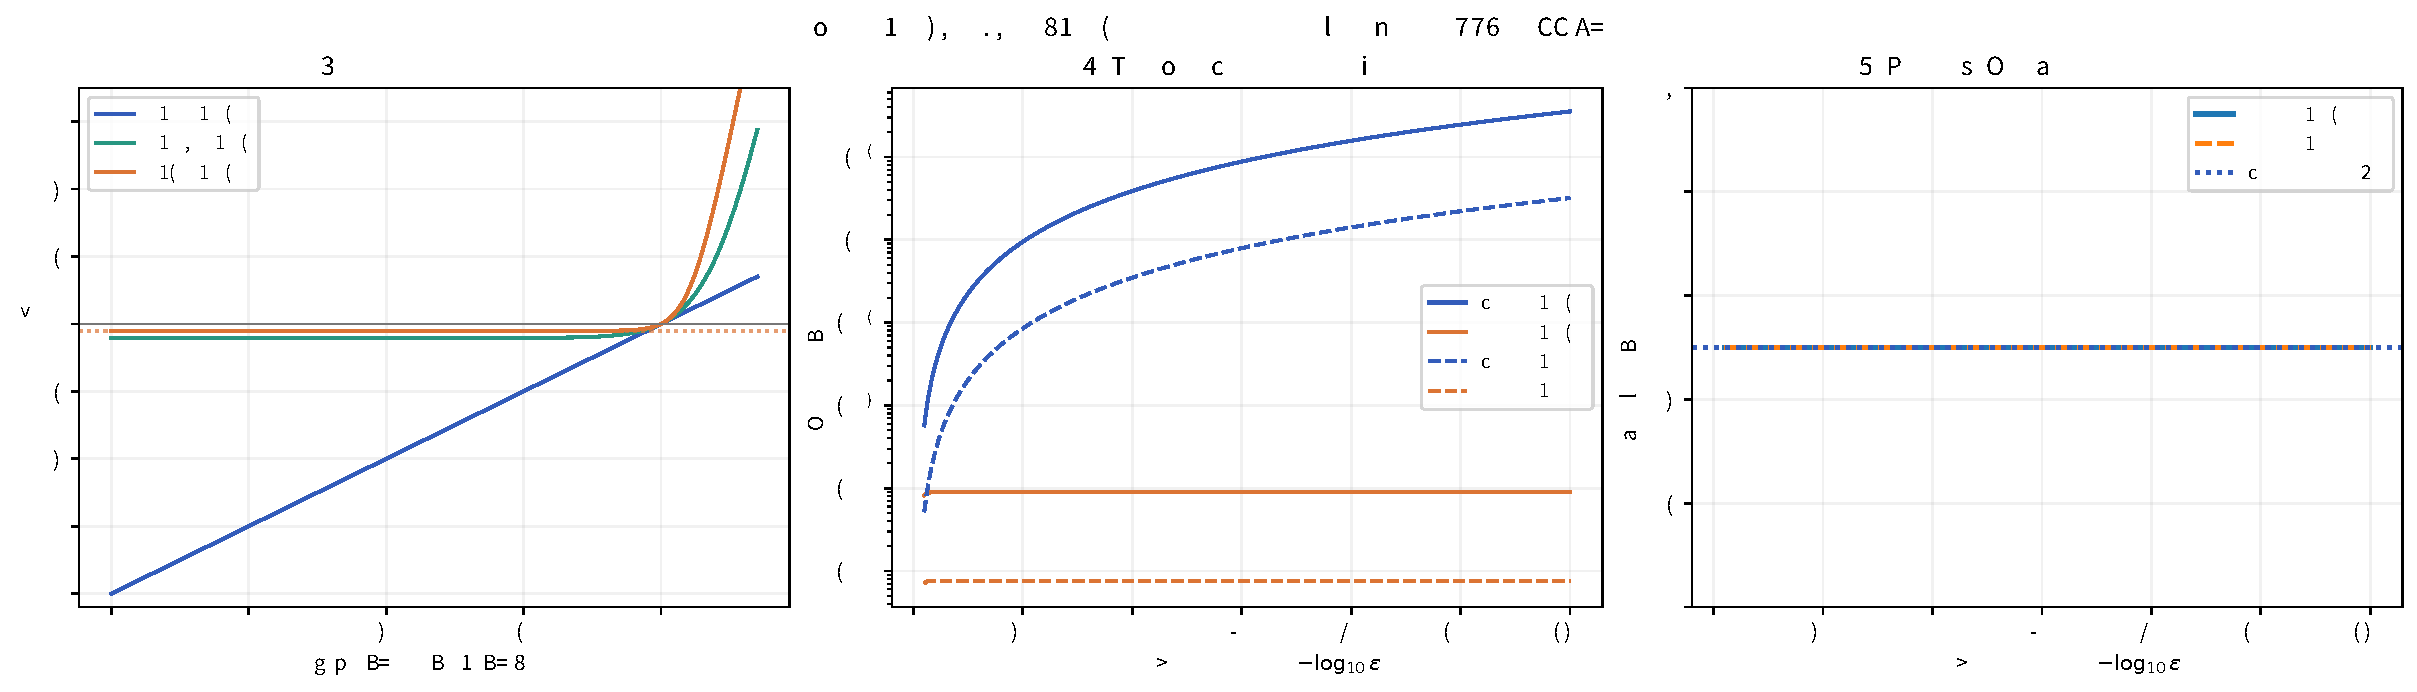
\includegraphics[width=\textwidth]{../../results/proximal-family-geometry/variance.pdf}
 \caption{尺度、尾部与标准化分别改变不同对象。早期图中 $\lambda$ 对应本章 $\eta$；中图使用 $q=(1/4,3/4)$ 的精确条件中心化 score 方差，右图验证二元标准差缩放的抵消现象。}
\end{figure}

\subsection{证明、解析图与实验记录的维护位置}

本章的图来自解析有限词表公式、已有模型缓存或已经登记的实验；正文与图注明确区分这些证据。重构只增加解析形状与反例图，不启动新的 GPU 训练。主线的 source、figure metadata 和确定性数值核验分别保存在 \path{docs/book/}、\path{results/chapter9-restructure/} 与对应第一方程序中。

原有几何、动力学和共享参数核验由 \path{experiments/analysis/proximal_family_geometry.py}、\path{experiments/analysis/proximal_family_dynamics.py} 生成。散度证书由 \path{experiments/analysis/power_generalization.py} 核验。中心和辅助采样的缓存审计位于 \path{results/power-center-advantage/} 与 \path{results/power-center-extensions/}。实际大模型 setting、结果和分析继续进入唯一实验报告，本章不复制待执行的 GPU 队列和运行流水。

% END SOURCE: sections/proximal_scope_summary.tex


% END SOURCE: chapters/09_proximal_families.tex

\backmatter
\chapter*{参考资料与来源}
\begingroup\raggedright
PMD-Mean 的 reward 中心化目标与 Lambert-$W$ 解依据 \href{https://arxiv.org/abs/2602.05933}{arXiv:2602.05933} 的目标定义及附录。本书重新给出完整的约束优化证明，并区分最优分布等价与梯度等价。
\par
K3$^{++}$、K4、K5、Top-$J$ 估计量的来源为 \href{https://arxiv.org/abs/2602.04417}{arXiv:2602.04417}。One-Shot-OPD 与 ResOPD 的版本及实现证据在实现章和实验章逐项说明。
\par\endgroup
\end{document}
